\subsection{Global parameters}
\label{parameters:global}


\begin{itemize}
\item {\it Parameter name:} {\tt Additional shared libraries}
\phantomsection\label{parameters:Additional shared libraries}
\label{parameters:Additional_20shared_20libraries}


\index[prmindex]{Additional shared libraries}
\index[prmindexfull]{Additional shared libraries}
{\it Value:} 


{\it Default:} 


{\it Description:} A list of names of additional shared libraries that should be loaded upon starting up the program. The names of these files can contain absolute or relative paths (relative to the directory in which you call ASPECT). In fact, file names that do not contain any directory information (i.e., only the name of a file such as $<$myplugin.so$>$ will not be found if they are not located in one of the directories listed in the \texttt{LD\_LIBRARY\_PATH} environment variable. In order to load a library in the current directory, use $<$./myplugin.so$>$ instead.

The typical use of this parameter is so that you can implement additional plugins in your own directories, rather than in the ASPECT source directories. You can then simply compile these plugins into a shared library without having to re-compile all of ASPECT. See the section of the manual discussing writing extensions for more information on how to compile additional files into a shared library.


{\it Possible values:} A list of 0 to 4294967295 elements where each element is [an input filename]
\item {\it Parameter name:} {\tt Adiabatic surface temperature}
\phantomsection\label{parameters:Adiabatic surface temperature}
\label{parameters:Adiabatic_20surface_20temperature}


\index[prmindex]{Adiabatic surface temperature}
\index[prmindexfull]{Adiabatic surface temperature}
{\it Value:} 0.


{\it Default:} 0.


{\it Description:} In order to make the problem in the first time step easier to solve, we need a reasonable guess for the temperature and pressure. To obtain it, we use an adiabatic pressure and temperature field. This parameter describes what the `adiabatic' temperature would be at the surface of the domain (i.e. at depth zero). Note that this value need not coincide with the boundary condition posed at this point. Rather, the boundary condition may differ significantly from the adiabatic value, and then typically induce a thermal boundary layer.

For more information, see the section in the manual that discusses the general mathematical model.


{\it Possible values:} A floating point number $v$ such that $-\text{MAX\_DOUBLE} \leq v \leq \text{MAX\_DOUBLE}$
\item {\it Parameter name:} {\tt CFL number}
\phantomsection\label{parameters:CFL number}
\label{parameters:CFL_20number}


\index[prmindex]{CFL number}
\index[prmindexfull]{CFL number}
{\it Value:} 1.0


{\it Default:} 1.0


{\it Description:} In computations, the time step $k$ is chosen according to $k = c \min_K \frac {h_K} {\|u\|_{\infty,K} p_T}$ where $h_K$ is the diameter of cell $K$, and the denominator is the maximal magnitude of the velocity on cell $K$ times the polynomial degree $p_T$ of the temperature discretization. The dimensionless constant $c$ is called the CFL number in this program. For time discretizations that have explicit components, $c$ must be less than a constant that depends on the details of the time discretization and that is no larger than one. On the other hand, for implicit discretizations such as the one chosen here, one can choose the time step as large as one wants (in particular, one can choose $c>1$) though a CFL number significantly larger than one will yield rather diffusive solutions. Units: None.


{\it Possible values:} A floating point number $v$ such that $0 \leq v \leq \text{MAX\_DOUBLE}$
\item {\it Parameter name:} {\tt Dimension}
\phantomsection\label{parameters:Dimension}


\index[prmindex]{Dimension}
\index[prmindexfull]{Dimension}
{\it Value:} 2


{\it Default:} 2


{\it Description:} The number of space dimensions you want to run this program in. ASPECT can run in 2 and 3 space dimensions.


{\it Possible values:} An integer $n$ such that $2\leq n \leq 3$
\item {\it Parameter name:} {\tt End time}
\phantomsection\label{parameters:End time}
\label{parameters:End_20time}


\index[prmindex]{End time}
\index[prmindexfull]{End time}
{\it Value:} 0.0


{\it Default:} 5.69e+300


{\it Description:} The end time of the simulation. The default value is a number so that when converted from years to seconds it is approximately equal to the largest number representable in floating point arithmetic. For all practical purposes, this equals infinity. Units: Years if the 'Use years in output instead of seconds' parameter is set; seconds otherwise.


{\it Possible values:} A floating point number $v$ such that $-\text{MAX\_DOUBLE} \leq v \leq \text{MAX\_DOUBLE}$
\item {\it Parameter name:} {\tt Max nonlinear iterations}
\phantomsection\label{parameters:Max nonlinear iterations}
\label{parameters:Max_20nonlinear_20iterations}


\index[prmindex]{Max nonlinear iterations}
\index[prmindexfull]{Max nonlinear iterations}
{\it Value:} 10


{\it Default:} 10


{\it Description:} The maximal number of nonlinear iterations to be performed.


{\it Possible values:} An integer $n$ such that $1\leq n \leq 2147483647$
\item {\it Parameter name:} {\tt Max nonlinear iterations in pre-refinement}
\phantomsection\label{parameters:Max nonlinear iterations in pre_2drefinement}
\label{parameters:Max_20nonlinear_20iterations_20in_20pre_2drefinement}


\index[prmindex]{Max nonlinear iterations in pre-refinement}
\index[prmindexfull]{Max nonlinear iterations in pre-refinement}
{\it Value:} 2147483647


{\it Default:} 2147483647


{\it Description:} The maximal number of nonlinear iterations to be performed in the pre-refinement steps. This does not include the last refinement step before moving to timestep 1. When this parameter has a larger value than max nonlinear iterations, the latter is used.


{\it Possible values:} An integer $n$ such that $0\leq n \leq 2147483647$
\item {\it Parameter name:} {\tt Maximum first time step}
\phantomsection\label{parameters:Maximum first time step}
\label{parameters:Maximum_20first_20time_20step}


\index[prmindex]{Maximum first time step}
\index[prmindexfull]{Maximum first time step}
{\it Value:} 5.69e+300


{\it Default:} 5.69e+300


{\it Description:} Set a maximum time step size for only the first timestep. Generally the time step based on the CFL number should be sufficient, but for complicated models or benchmarking it may be useful to limit the first time step to some value, especially when using the free surface, which needs to settle to prevent instabilities. This should in that case be combined with a value set for ``Maximum relative increase in time step''. The default value is a value so that when converted from years into seconds it equals the largest number representable by a floating point number, implying an unlimited time step. Units: Years or seconds, depending on the ``Use years in output instead of seconds'' parameter.


{\it Possible values:} A floating point number $v$ such that $0 \leq v \leq \text{MAX\_DOUBLE}$
\item {\it Parameter name:} {\tt Maximum relative increase in time step}
\phantomsection\label{parameters:Maximum relative increase in time step}
\label{parameters:Maximum_20relative_20increase_20in_20time_20step}


\index[prmindex]{Maximum relative increase in time step}
\index[prmindexfull]{Maximum relative increase in time step}
{\it Value:} 2147483647


{\it Default:} 2147483647


{\it Description:} Set a percentage with which the time step is limited to increase. Generally the time step based on the CFL number should be sufficient, but for complicated models which may suddenly drastically change behavior, it may be useful to limit the increase in the time step, without limiting the time step size of the whole simulation to a particular number. For example, if this parameter is set to $50$, then that means that the time step can at most increase by 50\% from one time step to the next, or by a factor of 1.5. Units: \%.


{\it Possible values:} A floating point number $v$ such that $0 \leq v \leq \text{MAX\_DOUBLE}$
\item {\it Parameter name:} {\tt Maximum time step}
\phantomsection\label{parameters:Maximum time step}
\label{parameters:Maximum_20time_20step}


\index[prmindex]{Maximum time step}
\index[prmindexfull]{Maximum time step}
{\it Value:} 5.69e+300


{\it Default:} 5.69e+300


{\it Description:} Set a maximum time step size for the solver to use. Generally the time step based on the CFL number should be sufficient, but for complicated models or benchmarking it may be useful to limit the time step to some value. The default value is a value so that when converted from years into seconds it equals the largest number representable by a floating point number, implying an unlimited time step.Units: Years or seconds, depending on the ``Use years in output instead of seconds'' parameter.


{\it Possible values:} A floating point number $v$ such that $0 \leq v \leq \text{MAX\_DOUBLE}$
\item {\it Parameter name:} {\tt Nonlinear solver scheme}
\phantomsection\label{parameters:Nonlinear solver scheme}
\label{parameters:Nonlinear_20solver_20scheme}


\index[prmindex]{Nonlinear solver scheme}
\index[prmindexfull]{Nonlinear solver scheme}
{\it Value:} single Advection, single Stokes


{\it Default:} single Advection, single Stokes


{\it Description:} The kind of scheme used to resolve the nonlinearity in the system. `single Advection, single Stokes' means that no nonlinear iterations are done, and the temperature, compositional fields and Stokes equations are solved exactly once per time step, one after the other. The `iterated Advection and Stokes' scheme iterates this decoupled approach by alternating the solution of the temperature, composition and Stokes systems. The `single Advection, iterated Stokes' scheme solves the temperature and composition equation once at the beginning of each time step and then iterates out the solution of the Stokes equation. The `no Advection, iterated Stokes' scheme only solves the Stokes system, iterating out the solution, and ignores compositions and the temperature equation (careful, the material model must not depend on the temperature or composition; this is mostly useful for Stokes benchmarks).  The `no Advection, single Stokes' scheme only solves the Stokes system once per timestep. This is also mostly useful for Stokes benchmarks. The `single Advection, no Stokes' scheme only solves the temperature and other advection systems once, and instead of solving for the Stokes system, a prescribed velocity and pressure is used. The `iterated Advection and Newton Stokes' scheme iterates by alternating the solution of the temperature, composition and Stokes equations, using Picard iterations for the temperature and composition, and Newton iterations for the Stokes system. The `single Advection, iterated Newton Stokes' scheme solves the temperature and composition equations once at the beginning of each time step and then iterates out the solution of the Stokes equation, using Newton iterations for the Stokes system. The `iterated Advection and defect correction Stokes' scheme iterates by alternating the solution of the temperature, composition and Stokes equations, using Picard iterations for the temperature and composition, and defect correction Picard iterations for the Stokes system. The `single Advection, iterated defect correction Stokes' scheme solves the temperature and composition equations once at the beginning of each time step and then iterates out the solution of the Stokes equation, using defect correction Picard iterations for the Stokes system. The `no Advection, iterated defect correction Stokes' scheme solves the temperature and composition equations once at the beginning of each time step and then iterates out the solution of the Stokes equation, using defect correction Picard iterations for the Stokes system. The `first timestep only, single Stokes' scheme solves the Stokes equations exactly once, at the first time step. No nonlinear iterations are done, and the temperature and composition systems are not solved. 

The `IMPES' scheme is deprecated and only allowed for reasons of backwards compatibility. It is the same as `single Advection, single Stokes' .The `iterated IMPES' scheme is deprecated and only allowed for reasons of backwards compatibility. It is the same as `iterated Advection and Stokes'. The `iterated Stokes' scheme is deprecated and only allowed for reasons of backwards compatibility. It is the same as `single Advection, iterated Stokes'. The `Stokes only' scheme is deprecated and only allowed for reasons of backwards compatibility. It is the same as `no Advection, iterated Stokes'. The `Advection only' scheme is deprecated and only allowed for reasons of backwards compatibility. It is the same as `single Advection, no Stokes'. The `Newton Stokes' scheme is deprecated and only allowed for reasons of backwards compatibility. It is the same as `iterated Advection and Newton Stokes'.


{\it Possible values:} Any one of single Advection, single Stokes, iterated Advection and Stokes, single Advection, iterated Stokes, no Advection, iterated Stokes, no Advection, single Stokes, no Advection, iterated defect correction Stokes, single Advection, iterated defect correction Stokes, iterated Advection and defect correction Stokes, iterated Advection and Newton Stokes, single Advection, iterated Newton Stokes, single Advection, no Stokes, IMPES, iterated IMPES, iterated Stokes, Newton Stokes, Stokes only, Advection only, first timestep only, single Stokes, no Advection, no Stokes
\item {\it Parameter name:} {\tt Nonlinear solver tolerance}
\phantomsection\label{parameters:Nonlinear solver tolerance}
\label{parameters:Nonlinear_20solver_20tolerance}


\index[prmindex]{Nonlinear solver tolerance}
\index[prmindexfull]{Nonlinear solver tolerance}
{\it Value:} 1e-5


{\it Default:} 1e-5


{\it Description:} A relative tolerance up to which the nonlinear solver will iterate. This parameter is only relevant if the `Nonlinear solver scheme' does nonlinear iterations, in other words, if it is set to something other than `single Advection, single Stokes' or `single Advection, no Stokes'.


{\it Possible values:} A floating point number $v$ such that $0 \leq v \leq 1$
\item {\it Parameter name:} {\tt Output directory}
\phantomsection\label{parameters:Output directory}
\label{parameters:Output_20directory}


\index[prmindex]{Output directory}
\index[prmindexfull]{Output directory}
{\it Value:} output


{\it Default:} output


{\it Description:} The name of the directory into which all output files should be placed. This may be an absolute or a relative path.


{\it Possible values:} A directory name
\item {\it Parameter name:} {\tt Pressure normalization}
\phantomsection\label{parameters:Pressure normalization}
\label{parameters:Pressure_20normalization}


\index[prmindex]{Pressure normalization}
\index[prmindexfull]{Pressure normalization}
{\it Value:} surface


{\it Default:} surface


{\it Description:} If and how to normalize the pressure after the solution step. This is necessary because depending on boundary conditions, in many cases the pressure is only determined by the model up to a constant. On the other hand, we often would like to have a well-determined pressure, for example for table lookups of material properties in models or for comparing solutions. If the given value is `surface', then normalization at the end of each time steps adds a constant value to the pressure in such a way that the average pressure at the surface of the domain is what is set in the `Surface pressure' parameter; the surface of the domain is determined by asking the geometry model whether a particular face of the geometry has a zero or small `depth'. If the value of this parameter is `volume' then the pressure is normalized so that the domain average is zero. If `no' is given, the no pressure normalization is performed.


{\it Possible values:} Any one of surface, volume, no
\item {\it Parameter name:} {\tt Resume computation}
\phantomsection\label{parameters:Resume computation}
\label{parameters:Resume_20computation}


\index[prmindex]{Resume computation}
\index[prmindexfull]{Resume computation}
{\it Value:} false


{\it Default:} false


{\it Description:} A flag indicating whether the computation should be resumed from a previously saved state (if true) or start from scratch (if false). If auto is selected, models will be resumed if there is an existing checkpoint file, otherwise started from scratch.


{\it Possible values:} Any one of true, false, auto
\item {\it Parameter name:} {\tt Start time}
\phantomsection\label{parameters:Start time}
\label{parameters:Start_20time}


\index[prmindex]{Start time}
\index[prmindexfull]{Start time}
{\it Value:} 0.


{\it Default:} 0.


{\it Description:} The start time of the simulation. Units: Years if the 'Use years in output instead of seconds' parameter is set; seconds otherwise.


{\it Possible values:} A floating point number $v$ such that $-\text{MAX\_DOUBLE} \leq v \leq \text{MAX\_DOUBLE}$
\item {\it Parameter name:} {\tt Surface pressure}
\phantomsection\label{parameters:Surface pressure}
\label{parameters:Surface_20pressure}


\index[prmindex]{Surface pressure}
\index[prmindexfull]{Surface pressure}
{\it Value:} 0.


{\it Default:} 0.


{\it Description:} The value the pressure is normalized to in each time step when `Pressure normalization' is set to `surface' with default value 0. This setting is ignored in all other cases.

The mathematical equations that describe thermal convection only determine the pressure up to an arbitrary constant. On the other hand, for comparison and for looking up material parameters it is important that the pressure be normalized somehow. We do this by enforcing a particular average pressure value at the surface of the domain, where the geometry model determines where the surface is. This parameter describes what this average surface pressure value is supposed to be. By default, it is set to zero, but one may want to choose a different value for example for simulating only the volume of the mantle below the lithosphere, in which case the surface pressure should be the lithostatic pressure at the bottom of the lithosphere.

For more information, see the section in the manual that discusses the general mathematical model.


{\it Possible values:} A floating point number $v$ such that $-\text{MAX\_DOUBLE} \leq v \leq \text{MAX\_DOUBLE}$
\item {\it Parameter name:} {\tt Timing output frequency}
\phantomsection\label{parameters:Timing output frequency}
\label{parameters:Timing_20output_20frequency}


\index[prmindex]{Timing output frequency}
\index[prmindexfull]{Timing output frequency}
{\it Value:} 100


{\it Default:} 100


{\it Description:} How frequently in timesteps to output timing information. This is generally adjusted only for debugging and timing purposes. If the value is set to zero it will also output timing information at the initiation timesteps.


{\it Possible values:} An integer $n$ such that $0\leq n \leq 2147483647$
\item {\it Parameter name:} {\tt Use conduction timestep}
\phantomsection\label{parameters:Use conduction timestep}
\label{parameters:Use_20conduction_20timestep}


\index[prmindex]{Use conduction timestep}
\index[prmindexfull]{Use conduction timestep}
{\it Value:} false


{\it Default:} false


{\it Description:} Mantle convection simulations are often focused on convection dominated systems. However, these codes can also be used to investigate systems where heat conduction plays a dominant role. This parameter indicates whether the simulator should also use heat conduction in determining the length of each time step.


{\it Possible values:} A boolean value (true or false)
\item {\it Parameter name:} {\tt Use operator splitting}
\phantomsection\label{parameters:Use operator splitting}
\label{parameters:Use_20operator_20splitting}


\index[prmindex]{Use operator splitting}
\index[prmindexfull]{Use operator splitting}
{\it Value:} false


{\it Default:} false


{\it Description:} If set to true, the advection and reactions of compositional fields and temperature are solved separately, and can use different time steps. Note that this will only work if the material/heating model fills the reaction\_rates/heating\_reaction\_rates structures. Operator splitting can be used with any existing solver schemes that solve the temperature/composition equations.


{\it Possible values:} A boolean value (true or false)
\item {\it Parameter name:} {\tt Use years in output instead of seconds}
\phantomsection\label{parameters:Use years in output instead of seconds}
\label{parameters:Use_20years_20in_20output_20instead_20of_20seconds}


\index[prmindex]{Use years in output instead of seconds}
\index[prmindexfull]{Use years in output instead of seconds}
{\it Value:} true


{\it Default:} true


{\it Description:} When computing results for mantle convection simulations, it is often difficult to judge the order of magnitude of results when they are stated in MKS units involving seconds. Rather, some kinds of results such as velocities are often stated in terms of meters per year (or, sometimes, centimeters per year). On the other hand, for non-dimensional computations, one wants results in their natural unit system as used inside the code. If this flag is set to `true' conversion to years happens; if it is `false', no such conversion happens.

Contrary to the word ``output'' in the name of this parameter, a number of plugins also use this parameter to determine how to interpret their \textit{inputs}. For example, when `true', several of the boundary velocity models described in Section~\ref{parameters:Boundary_20velocity_20model} interpret both specific times in years instead of seconds, and velocities in meters per year instead of meters per second.


{\it Possible values:} A boolean value (true or false)
\item {\it Parameter name:} {\tt World builder file}
\phantomsection\label{parameters:World builder file}
\label{parameters:World_20builder_20file}


\index[prmindex]{World builder file}
\index[prmindexfull]{World builder file}
{\it Value:} 


{\it Default:} 


{\it Description:} Name of the world builder file. If empty, the world builder is not initialized.


{\it Possible values:} an input filename
\end{itemize}



\subsection{Parameters in section \tt Adiabatic conditions model}
\label{parameters:Adiabatic_20conditions_20model}

\begin{itemize}
\item {\it Parameter name:} {\tt Model name}
\phantomsection\label{parameters:Adiabatic conditions model/Model name}
\label{parameters:Adiabatic_20conditions_20model/Model_20name}


\index[prmindex]{Model name}
\index[prmindexfull]{Adiabatic conditions model!Model name}
{\it Value:} compute profile


{\it Default:} compute profile


{\it Description:} Select one of the following models:

`ascii data': A model in which the adiabatic profile is read from a file that describes the reference state. Note the required format of the input data: The first lines may contain any number of comments if they begin with `\#', but one of these lines needs to contain the number of points in the reference state as for example `\# POINTS: 3'. Following the comment lines there has to be a single line containing the names of all data columns, separated by arbitrarily many spaces. Column names are not allowed to contain spaces. The file can contain unnecessary columns, but for this plugin it needs to at least provide columns named `temperature', `pressure', and `density'. Note that the data lines in the file need to be sorted in order of increasing depth from 0 to the maximal depth in the model domain. Points in the model that are outside of the provided depth range will be assigned the maximum or minimum depth values, respectively. Points do not need to be equidistant, but the computation of properties is optimized in speed if they are.

`compute profile': A model in which the adiabatic profile is calculated by solving the hydrostatic equations for pressure and temperature in depth. The gravity is assumed to be in depth direction and the composition is either given by the initial composition at reference points or computed as a reference depth-function. All material parameters are computed by the material model plugin. The surface conditions are either constant or changing over time as prescribed by a user-provided function.

`function': A model in which the adiabatic profile is specified by a user defined function. The supplied function has to contain temperature, pressure, and density as a function of depth in this order.


{\it Possible values:} Any one of ascii data, compute profile, function
\end{itemize}



\subsection{Parameters in section \tt Adiabatic conditions model/Ascii data model}
\label{parameters:Adiabatic_20conditions_20model/Ascii_20data_20model}

\begin{itemize}
\item {\it Parameter name:} {\tt Data directory}
\phantomsection\label{parameters:Adiabatic conditions model/Ascii data model/Data directory}
\label{parameters:Adiabatic_20conditions_20model/Ascii_20data_20model/Data_20directory}


\index[prmindex]{Data directory}
\index[prmindexfull]{Adiabatic conditions model!Ascii data model!Data directory}
{\it Value:} \$ASPECT\_SOURCE\_DIR/tests/adiabatic-conditions/ascii-data/test/


{\it Default:} \$ASPECT\_SOURCE\_DIR/tests/adiabatic-conditions/ascii-data/test/


{\it Description:} The name of a directory that contains the model data. This path may either be absolute (if starting with a `/') or relative to the current directory. The path may also include the special text `\$ASPECT\_SOURCE\_DIR' which will be interpreted as the path in which the ASPECT source files were located when ASPECT was compiled. This interpretation allows, for example, to reference files located in the `data/' subdirectory of ASPECT.


{\it Possible values:} A directory name
\item {\it Parameter name:} {\tt Data file name}
\phantomsection\label{parameters:Adiabatic conditions model/Ascii data model/Data file name}
\label{parameters:Adiabatic_20conditions_20model/Ascii_20data_20model/Data_20file_20name}


\index[prmindex]{Data file name}
\index[prmindexfull]{Adiabatic conditions model!Ascii data model!Data file name}
{\it Value:} 


{\it Default:} 


{\it Description:} The file name of the model data.


{\it Possible values:} Any string
\item {\it Parameter name:} {\tt Scale factor}
\phantomsection\label{parameters:Adiabatic conditions model/Ascii data model/Scale factor}
\label{parameters:Adiabatic_20conditions_20model/Ascii_20data_20model/Scale_20factor}


\index[prmindex]{Scale factor}
\index[prmindexfull]{Adiabatic conditions model!Ascii data model!Scale factor}
{\it Value:} 1.


{\it Default:} 1.


{\it Description:} Scalar factor, which is applied to the model data. You might want to use this to scale the input to a reference model. Another way to use this factor is to convert units of the input files. For instance, if you provide velocities in cm/yr set this factor to 0.01.


{\it Possible values:} A floating point number $v$ such that $-\text{MAX\_DOUBLE} \leq v \leq \text{MAX\_DOUBLE}$
\end{itemize}

\subsection{Parameters in section \tt Adiabatic conditions model/Compute profile}
\label{parameters:Adiabatic_20conditions_20model/Compute_20profile}

\begin{itemize}
\item {\it Parameter name:} {\tt Composition reference profile}
\phantomsection\label{parameters:Adiabatic conditions model/Compute profile/Composition reference profile}
\label{parameters:Adiabatic_20conditions_20model/Compute_20profile/Composition_20reference_20profile}


\index[prmindex]{Composition reference profile}
\index[prmindexfull]{Adiabatic conditions model!Compute profile!Composition reference profile}
{\it Value:} initial composition


{\it Default:} initial composition


{\it Description:} Select how the reference profile for composition is computed. This profile is used to evaluate the material model, when computing the pressure and temperature profile.


{\it Possible values:} Any one of initial composition, function
\item {\it Parameter name:} {\tt Function constants}
\phantomsection\label{parameters:Adiabatic conditions model/Compute profile/Function constants}
\label{parameters:Adiabatic_20conditions_20model/Compute_20profile/Function_20constants}


\index[prmindex]{Function constants}
\index[prmindexfull]{Adiabatic conditions model!Compute profile!Function constants}
{\it Value:} 


{\it Default:} 


{\it Description:} Sometimes it is convenient to use symbolic constants in the expression that describes the function, rather than having to use its numeric value everywhere the constant appears. These values can be defined using this parameter, in the form `var1=value1, var2=value2, ...'.

A typical example would be to set this runtime parameter to `pi=3.1415926536' and then use `pi' in the expression of the actual formula. (That said, for convenience this class actually defines both `pi' and `Pi' by default, but you get the idea.)


{\it Possible values:} Any string
\item {\it Parameter name:} {\tt Function expression}
\phantomsection\label{parameters:Adiabatic conditions model/Compute profile/Function expression}
\label{parameters:Adiabatic_20conditions_20model/Compute_20profile/Function_20expression}


\index[prmindex]{Function expression}
\index[prmindexfull]{Adiabatic conditions model!Compute profile!Function expression}
{\it Value:} 0


{\it Default:} 0


{\it Description:} The formula that denotes the function you want to evaluate for particular values of the independent variables. This expression may contain any of the usual operations such as addition or multiplication, as well as all of the common functions such as `sin' or `cos'. In addition, it may contain expressions like `if(x>0, 1, -1)' where the expression evaluates to the second argument if the first argument is true, and to the third argument otherwise. For a full overview of possible expressions accepted see the documentation of the muparser library at http://muparser.beltoforion.de/.

If the function you are describing represents a vector-valued function with multiple components, then separate the expressions for individual components by a semicolon.


{\it Possible values:} Any string
\item {\it Parameter name:} {\tt Number of points}
\phantomsection\label{parameters:Adiabatic conditions model/Compute profile/Number of points}
\label{parameters:Adiabatic_20conditions_20model/Compute_20profile/Number_20of_20points}


\index[prmindex]{Number of points}
\index[prmindexfull]{Adiabatic conditions model!Compute profile!Number of points}
{\it Value:} 1000


{\it Default:} 1000


{\it Description:} The number of points we use to compute the adiabatic profile. The higher the number of points, the more accurate the downward integration from the adiabatic surface temperature will be.


{\it Possible values:} An integer $n$ such that $5\leq n \leq 2147483647$
\item {\it Parameter name:} {\tt Use surface condition function}
\phantomsection\label{parameters:Adiabatic conditions model/Compute profile/Use surface condition function}
\label{parameters:Adiabatic_20conditions_20model/Compute_20profile/Use_20surface_20condition_20function}


\index[prmindex]{Use surface condition function}
\index[prmindexfull]{Adiabatic conditions model!Compute profile!Use surface condition function}
{\it Value:} false


{\it Default:} false


{\it Description:} Whether to use the 'Surface condition function' to determine surface conditions, or the 'Adiabatic surface temperature' and 'Surface pressure' parameters. If this is set to true the reference profile is updated every timestep. The function expression of the function should be independent of space, but can depend on time 't'. The function must return two components, the first one being reference surface pressure, the second one being reference surface temperature.


{\it Possible values:} A boolean value (true or false)
\item {\it Parameter name:} {\tt Variable names}
\phantomsection\label{parameters:Adiabatic conditions model/Compute profile/Variable names}
\label{parameters:Adiabatic_20conditions_20model/Compute_20profile/Variable_20names}


\index[prmindex]{Variable names}
\index[prmindexfull]{Adiabatic conditions model!Compute profile!Variable names}
{\it Value:} x,t


{\it Default:} x,t


{\it Description:} The names of the variables as they will be used in the function, separated by commas. By default, the names of variables at which the function will be evaluated are `x' (in 1d), `x,y' (in 2d) or `x,y,z' (in 3d) for spatial coordinates and `t' for time. You can then use these variable names in your function expression and they will be replaced by the values of these variables at which the function is currently evaluated. However, you can also choose a different set of names for the independent variables at which to evaluate your function expression. For example, if you work in spherical coordinates, you may wish to set this input parameter to `r,phi,theta,t' and then use these variable names in your function expression.


{\it Possible values:} Any string
\end{itemize}



\subsection{Parameters in section \tt Adiabatic conditions model/Compute profile/Surface condition function}
\label{parameters:Adiabatic_20conditions_20model/Compute_20profile/Surface_20condition_20function}

\begin{itemize}
\item {\it Parameter name:} {\tt Function constants}
\phantomsection\label{parameters:Adiabatic conditions model/Compute profile/Surface condition function/Function constants}
\label{parameters:Adiabatic_20conditions_20model/Compute_20profile/Surface_20condition_20function/Function_20constants}


\index[prmindex]{Function constants}
\index[prmindexfull]{Adiabatic conditions model!Compute profile!Surface condition function/Function constants}
{\it Value:} 


{\it Default:} 


{\it Description:} Sometimes it is convenient to use symbolic constants in the expression that describes the function, rather than having to use its numeric value everywhere the constant appears. These values can be defined using this parameter, in the form `var1=value1, var2=value2, ...'.

A typical example would be to set this runtime parameter to `pi=3.1415926536' and then use `pi' in the expression of the actual formula. (That said, for convenience this class actually defines both `pi' and `Pi' by default, but you get the idea.)


{\it Possible values:} Any string
\item {\it Parameter name:} {\tt Function expression}
\phantomsection\label{parameters:Adiabatic conditions model/Compute profile/Surface condition function/Function expression}
\label{parameters:Adiabatic_20conditions_20model/Compute_20profile/Surface_20condition_20function/Function_20expression}


\index[prmindex]{Function expression}
\index[prmindexfull]{Adiabatic conditions model!Compute profile!Surface condition function/Function expression}
{\it Value:} 0; 0


{\it Default:} 0; 0


{\it Description:} The formula that denotes the function you want to evaluate for particular values of the independent variables. This expression may contain any of the usual operations such as addition or multiplication, as well as all of the common functions such as `sin' or `cos'. In addition, it may contain expressions like `if(x>0, 1, -1)' where the expression evaluates to the second argument if the first argument is true, and to the third argument otherwise. For a full overview of possible expressions accepted see the documentation of the muparser library at http://muparser.beltoforion.de/.

If the function you are describing represents a vector-valued function with multiple components, then separate the expressions for individual components by a semicolon.


{\it Possible values:} Any string
\item {\it Parameter name:} {\tt Variable names}
\phantomsection\label{parameters:Adiabatic conditions model/Compute profile/Surface condition function/Variable names}
\label{parameters:Adiabatic_20conditions_20model/Compute_20profile/Surface_20condition_20function/Variable_20names}


\index[prmindex]{Variable names}
\index[prmindexfull]{Adiabatic conditions model!Compute profile!Surface condition function/Variable names}
{\it Value:} x,t


{\it Default:} x,t


{\it Description:} The names of the variables as they will be used in the function, separated by commas. By default, the names of variables at which the function will be evaluated are `x' (in 1d), `x,y' (in 2d) or `x,y,z' (in 3d) for spatial coordinates and `t' for time. You can then use these variable names in your function expression and they will be replaced by the values of these variables at which the function is currently evaluated. However, you can also choose a different set of names for the independent variables at which to evaluate your function expression. For example, if you work in spherical coordinates, you may wish to set this input parameter to `r,phi,theta,t' and then use these variable names in your function expression.


{\it Possible values:} Any string
\end{itemize}

\subsection{Parameters in section \tt Adiabatic conditions model/Function}
\label{parameters:Adiabatic_20conditions_20model/Function}

\begin{itemize}
\item {\it Parameter name:} {\tt Function constants}
\phantomsection\label{parameters:Adiabatic conditions model/Function/Function constants}
\label{parameters:Adiabatic_20conditions_20model/Function/Function_20constants}


\index[prmindex]{Function constants}
\index[prmindexfull]{Adiabatic conditions model!Function!Function constants}
{\it Value:} 


{\it Default:} 


{\it Description:} Sometimes it is convenient to use symbolic constants in the expression that describes the function, rather than having to use its numeric value everywhere the constant appears. These values can be defined using this parameter, in the form `var1=value1, var2=value2, ...'.

A typical example would be to set this runtime parameter to `pi=3.1415926536' and then use `pi' in the expression of the actual formula. (That said, for convenience this class actually defines both `pi' and `Pi' by default, but you get the idea.)


{\it Possible values:} Any string
\item {\it Parameter name:} {\tt Function expression}
\phantomsection\label{parameters:Adiabatic conditions model/Function/Function expression}
\label{parameters:Adiabatic_20conditions_20model/Function/Function_20expression}


\index[prmindex]{Function expression}
\index[prmindexfull]{Adiabatic conditions model!Function!Function expression}
{\it Value:} 0.0; 0.0; 1.0


{\it Default:} 0.0; 0.0; 1.0


{\it Description:} Expression for the adiabatic temperature, pressure, and density separated by semicolons as a function of `depth'.


{\it Possible values:} Any string
\item {\it Parameter name:} {\tt Variable names}
\phantomsection\label{parameters:Adiabatic conditions model/Function/Variable names}
\label{parameters:Adiabatic_20conditions_20model/Function/Variable_20names}


\index[prmindex]{Variable names}
\index[prmindexfull]{Adiabatic conditions model!Function!Variable names}
{\it Value:} depth


{\it Default:} depth


{\it Possible values:} Any string
\end{itemize}

\subsection{Parameters in section \tt Boundary composition model}
\label{parameters:Boundary_20composition_20model}

\begin{itemize}
\item {\it Parameter name:} {\tt Allow fixed composition on outflow boundaries}
\phantomsection\label{parameters:Boundary composition model/Allow fixed composition on outflow boundaries}
\label{parameters:Boundary_20composition_20model/Allow_20fixed_20composition_20on_20outflow_20boundaries}


\index[prmindex]{Allow fixed composition on outflow boundaries}
\index[prmindexfull]{Boundary composition model!Allow fixed composition on outflow boundaries}
{\it Value:} false for models without melt


{\it Default:} false for models without melt


{\it Description:} When the composition is fixed on a given boundary as determined by the list of 'Fixed composition boundary indicators', there might be parts of the boundary where material flows out and one may want to prescribe the composition only on those parts of the boundary where there is inflow. This parameter determines if compositions are only prescribed at these inflow parts of the boundary (if false) or everywhere on a given boundary, independent of the flow direction (if true). By default, this parameter is set to false, except in models with melt transport (see below). Note that in this context, `fixed' refers to the fact that these are the boundary indicators where Dirichlet boundary conditions are applied, and does not imply that the boundary composition is time-independent. 

Mathematically speaking, the compositional fields satisfy an advection equation that has no diffusion. For this equation, one can only impose Dirichlet boundary conditions (i.e., prescribe a fixed compositional field value at the boundary) at those boundaries where material flows in. This would correspond to the ``false'' setting of this parameter, which is correspondingly the default. On the other hand, on a finite dimensional discretization such as the one one obtains from the finite element method, it is possible to also prescribe values on outflow boundaries, even though this may make no physical sense. This would then correspond to the ``true'' setting of this parameter. Note however that this parameter is only taken into account for the continuous field method and is not applied to the Discontinuous Galerkin (DG) field method. 

A warning for models with melt transport: In models with fluid flow, some compositional fields (in particular the porosity) might be transported with the fluid velocity, and would need to set the constraints based on the fluid velocity. However, this is currently not possible, because we reuse the same matrix for all compositional fields, and therefore can not use different constraints for different fields. Consequently, we set this parameter to true by default in models where melt transport is enabled. Be aware that if you change this default setting, you will not use the melt velocity, but the solid velocity to determine on which parts of the boundaries there is outflow.


{\it Possible values:} Any one of true, false, false for models without melt
\item {\it Parameter name:} {\tt Fixed composition boundary indicators}
\phantomsection\label{parameters:Boundary composition model/Fixed composition boundary indicators}
\label{parameters:Boundary_20composition_20model/Fixed_20composition_20boundary_20indicators}


\index[prmindex]{Fixed composition boundary indicators}
\index[prmindexfull]{Boundary composition model!Fixed composition boundary indicators}
{\it Value:} 


{\it Default:} 


{\it Description:} A comma separated list of names denoting those boundaries on which the composition is fixed and described by the boundary composition object selected in its own section of this input file. All boundary indicators used by the geometry but not explicitly listed here will end up with no-flux (insulating) boundary conditions.

The names of the boundaries listed here can either be numbers (in which case they correspond to the numerical boundary indicators assigned by the geometry object), or they can correspond to any of the symbolic names the geometry object may have provided for each part of the boundary. You may want to compare this with the documentation of the geometry model you use in your model.

This parameter only describes which boundaries have a fixed composition, but not what composition should hold on these boundaries. The latter piece of information needs to be implemented in a plugin in the BoundaryComposition group, unless an existing implementation in this group already provides what you want.


{\it Possible values:} A list of 0 to 4294967295 elements where each element is [Any string]
\item {\it Parameter name:} {\tt List of model names}
\phantomsection\label{parameters:Boundary composition model/List of model names}
\label{parameters:Boundary_20composition_20model/List_20of_20model_20names}


\index[prmindex]{List of model names}
\index[prmindexfull]{Boundary composition model!List of model names}
{\it Value:} 


{\it Default:} 


{\it Description:} A comma-separated list of boundary composition models that will be used to initialize the composition. These plugins are loaded in the order given, and modify the existing composition field via the operators listed in 'List of model operators'.

The following boundary composition models are available:

`ascii data': Implementation of a model in which the boundary composition is derived from files containing data in ascii format. Note the required format of the input data: The first lines may contain any number of comments if they begin with `\#', but one of these lines needs to contain the number of grid points in each dimension as for example `\# POINTS: 3 3'. The order of the data columns has to be `x', `composition1', `composition2', etc. in a 2d model and `x', `y', `composition1', `composition2', etc., in a 3d model, according to the number of compositional fields, which means that there has to be a single column for every composition in the model. Note that the data in the input files need to be sorted in a specific order: the first coordinate needs to ascend first, followed by the second in order to assign the correct data to the prescribed coordinates.If you use a spherical model, then the assumed grid changes. `x' will be replaced by the radial distance of the point to the bottom of the model, `y' by the azimuth angle and `z' by the polar angle measured positive from the north pole. The grid will be assumed to be a latitude-longitude grid. Note that the order of spherical coordinates is `r', `phi', `theta' and not `r', `theta', `phi', since this allows for dimension independent expressions.

`box': A model in which the composition is chosen constant on the sides of a box which are selected by the parameters Left/Right/Top/Bottom/Front/Back composition

`box with lithosphere boundary indicators': A model in which the composition is chosen constant on all the sides of a box. Additional boundary indicators are added to the lithospheric parts of the vertical boundaries. This model is to be used with the 'Two Merged Boxes' Geometry Model.

`function': Implementation of a model in which the boundary composition is given in terms of an explicit formula that is elaborated in the parameters in section ``Boundary composition model|Function''. 

Since the symbol $t$ indicating time may appear in the formulas for the prescribed composition, it is interpreted as having units seconds unless the global input parameter ``Use years in output instead of seconds'' is set, in which case we interpret the formula expressions as having units year.

The format of these functions follows the syntax understood by the muparser library, see Section~\ref{sec:muparser-format}.

`initial composition': A model in which the composition at the boundary is chosen to be the same as given in the initial conditions.

Because this class simply takes what the initial composition had described, this class can not know certain pieces of information such as the minimal and maximal composition on the boundary. For operations that require this, for example in post-processing, this boundary composition model must therefore be told what the minimal and maximal values on the boundary are. This is done using parameters set in section ``Boundary composition model/Initial composition''.

`spherical constant': A model in which the composition is chosen constant on the inner and outer boundaries of a surface, spherical shell, chunk or ellipsoidal chunk. Parameters are read from subsection 'Spherical constant'.


{\it Possible values:} A comma-separated list of any of ascii data, box, box with lithosphere boundary indicators, function, initial composition, spherical constant
\item {\it Parameter name:} {\tt List of model operators}
\phantomsection\label{parameters:Boundary composition model/List of model operators}
\label{parameters:Boundary_20composition_20model/List_20of_20model_20operators}


\index[prmindex]{List of model operators}
\index[prmindexfull]{Boundary composition model!List of model operators}
{\it Value:} add


{\it Default:} add


{\it Description:} A comma-separated list of operators that will be used to append the listed composition models onto the previous models. If only one operator is given, the same operator is applied to all models.


{\it Possible values:} A comma-separated list of any of add, subtract, minimum, maximum, replace if valid
\item {\it Parameter name:} {\tt Model name}
\phantomsection\label{parameters:Boundary composition model/Model name}
\label{parameters:Boundary_20composition_20model/Model_20name}


\index[prmindex]{Model name}
\index[prmindexfull]{Boundary composition model!Model name}
{\it Value:} unspecified


{\it Default:} unspecified


{\it Description:} Select one of the following models:

`ascii data': Implementation of a model in which the boundary composition is derived from files containing data in ascii format. Note the required format of the input data: The first lines may contain any number of comments if they begin with `\#', but one of these lines needs to contain the number of grid points in each dimension as for example `\# POINTS: 3 3'. The order of the data columns has to be `x', `composition1', `composition2', etc. in a 2d model and `x', `y', `composition1', `composition2', etc., in a 3d model, according to the number of compositional fields, which means that there has to be a single column for every composition in the model. Note that the data in the input files need to be sorted in a specific order: the first coordinate needs to ascend first, followed by the second in order to assign the correct data to the prescribed coordinates.If you use a spherical model, then the assumed grid changes. `x' will be replaced by the radial distance of the point to the bottom of the model, `y' by the azimuth angle and `z' by the polar angle measured positive from the north pole. The grid will be assumed to be a latitude-longitude grid. Note that the order of spherical coordinates is `r', `phi', `theta' and not `r', `theta', `phi', since this allows for dimension independent expressions.

`box': A model in which the composition is chosen constant on the sides of a box which are selected by the parameters Left/Right/Top/Bottom/Front/Back composition

`box with lithosphere boundary indicators': A model in which the composition is chosen constant on all the sides of a box. Additional boundary indicators are added to the lithospheric parts of the vertical boundaries. This model is to be used with the 'Two Merged Boxes' Geometry Model.

`function': Implementation of a model in which the boundary composition is given in terms of an explicit formula that is elaborated in the parameters in section ``Boundary composition model|Function''. 

Since the symbol $t$ indicating time may appear in the formulas for the prescribed composition, it is interpreted as having units seconds unless the global input parameter ``Use years in output instead of seconds'' is set, in which case we interpret the formula expressions as having units year.

The format of these functions follows the syntax understood by the muparser library, see Section~\ref{sec:muparser-format}.

`initial composition': A model in which the composition at the boundary is chosen to be the same as given in the initial conditions.

Because this class simply takes what the initial composition had described, this class can not know certain pieces of information such as the minimal and maximal composition on the boundary. For operations that require this, for example in post-processing, this boundary composition model must therefore be told what the minimal and maximal values on the boundary are. This is done using parameters set in section ``Boundary composition model/Initial composition''.

`spherical constant': A model in which the composition is chosen constant on the inner and outer boundaries of a surface, spherical shell, chunk or ellipsoidal chunk. Parameters are read from subsection 'Spherical constant'.

\textbf{Warning}: This parameter provides an old and deprecated way of specifying boundary composition models and shouldn't be used. Please use 'List of model names' instead.


{\it Possible values:} Any one of ascii data, box, box with lithosphere boundary indicators, function, initial composition, spherical constant, unspecified
\end{itemize}



\subsection{Parameters in section \tt Boundary composition model/Ascii data model}
\label{parameters:Boundary_20composition_20model/Ascii_20data_20model}

\begin{itemize}
\item {\it Parameter name:} {\tt Data directory}
\phantomsection\label{parameters:Boundary composition model/Ascii data model/Data directory}
\label{parameters:Boundary_20composition_20model/Ascii_20data_20model/Data_20directory}


\index[prmindex]{Data directory}
\index[prmindexfull]{Boundary composition model!Ascii data model!Data directory}
{\it Value:} \$ASPECT\_SOURCE\_DIR/data/boundary-composition/ascii-data/test/


{\it Default:} \$ASPECT\_SOURCE\_DIR/data/boundary-composition/ascii-data/test/


{\it Description:} The name of a directory that contains the model data. This path may either be absolute (if starting with a `/') or relative to the current directory. The path may also include the special text `\$ASPECT\_SOURCE\_DIR' which will be interpreted as the path in which the ASPECT source files were located when ASPECT was compiled. This interpretation allows, for example, to reference files located in the `data/' subdirectory of ASPECT.


{\it Possible values:} A directory name
\item {\it Parameter name:} {\tt Data file name}
\phantomsection\label{parameters:Boundary composition model/Ascii data model/Data file name}
\label{parameters:Boundary_20composition_20model/Ascii_20data_20model/Data_20file_20name}


\index[prmindex]{Data file name}
\index[prmindexfull]{Boundary composition model!Ascii data model!Data file name}
{\it Value:} box\_2d\_\%s.\%d.txt


{\it Default:} box\_2d\_\%s.\%d.txt


{\it Description:} The file name of the model data. Provide file in format: (File name).\%s\%d, where \%s is a string specifying the boundary of the model according to the names of the boundary indicators (of the chosen geometry model), and \%d is any sprintf integer qualifier specifying the format of the current file number.


{\it Possible values:} Any string
\item {\it Parameter name:} {\tt Data file time step}
\phantomsection\label{parameters:Boundary composition model/Ascii data model/Data file time step}
\label{parameters:Boundary_20composition_20model/Ascii_20data_20model/Data_20file_20time_20step}


\index[prmindex]{Data file time step}
\index[prmindexfull]{Boundary composition model!Ascii data model!Data file time step}
{\it Value:} 1e6


{\it Default:} 1e6


{\it Description:} Time step between following data files. Depending on the setting of the global `Use years in output instead of seconds' flag in the input file, this number is either interpreted as seconds or as years. The default is one million, i.e., either one million seconds or one million years.


{\it Possible values:} A floating point number $v$ such that $0 \leq v \leq \text{MAX\_DOUBLE}$
\item {\it Parameter name:} {\tt Decreasing file order}
\phantomsection\label{parameters:Boundary composition model/Ascii data model/Decreasing file order}
\label{parameters:Boundary_20composition_20model/Ascii_20data_20model/Decreasing_20file_20order}


\index[prmindex]{Decreasing file order}
\index[prmindexfull]{Boundary composition model!Ascii data model!Decreasing file order}
{\it Value:} false


{\it Default:} false


{\it Description:} In some cases the boundary files are not numbered in increasing but in decreasing order (e.g. `Ma BP'). If this flag is set to `True' the plugin will first load the file with the number `First data file number' and decrease the file number during the model run.


{\it Possible values:} A boolean value (true or false)
\item {\it Parameter name:} {\tt First data file model time}
\phantomsection\label{parameters:Boundary composition model/Ascii data model/First data file model time}
\label{parameters:Boundary_20composition_20model/Ascii_20data_20model/First_20data_20file_20model_20time}


\index[prmindex]{First data file model time}
\index[prmindexfull]{Boundary composition model!Ascii data model!First data file model time}
{\it Value:} 0


{\it Default:} 0


{\it Description:} The `First data file model time' parameter has been deactivated and will be removed in a future release. Do not use this paramter and instead provide data files starting from the model start time.


{\it Possible values:} A floating point number $v$ such that $0 \leq v \leq \text{MAX\_DOUBLE}$
\item {\it Parameter name:} {\tt First data file number}
\phantomsection\label{parameters:Boundary composition model/Ascii data model/First data file number}
\label{parameters:Boundary_20composition_20model/Ascii_20data_20model/First_20data_20file_20number}


\index[prmindex]{First data file number}
\index[prmindexfull]{Boundary composition model!Ascii data model!First data file number}
{\it Value:} 0


{\it Default:} 0


{\it Description:} Number of the first velocity file to be loaded when the model time is larger than `First velocity file model time'.


{\it Possible values:} An integer $n$ such that $-2147483648\leq n \leq 2147483647$
\item {\it Parameter name:} {\tt Scale factor}
\phantomsection\label{parameters:Boundary composition model/Ascii data model/Scale factor}
\label{parameters:Boundary_20composition_20model/Ascii_20data_20model/Scale_20factor}


\index[prmindex]{Scale factor}
\index[prmindexfull]{Boundary composition model!Ascii data model!Scale factor}
{\it Value:} 1.


{\it Default:} 1.


{\it Description:} Scalar factor, which is applied to the model data. You might want to use this to scale the input to a reference model. Another way to use this factor is to convert units of the input files. For instance, if you provide velocities in cm/yr set this factor to 0.01.


{\it Possible values:} A floating point number $v$ such that $-\text{MAX\_DOUBLE} \leq v \leq \text{MAX\_DOUBLE}$
\end{itemize}

\subsection{Parameters in section \tt Boundary composition model/Box}
\label{parameters:Boundary_20composition_20model/Box}

\begin{itemize}
\item {\it Parameter name:} {\tt Bottom composition}
\phantomsection\label{parameters:Boundary composition model/Box/Bottom composition}
\label{parameters:Boundary_20composition_20model/Box/Bottom_20composition}


\index[prmindex]{Bottom composition}
\index[prmindexfull]{Boundary composition model!Box!Bottom composition}
{\it Value:} 


{\it Default:} 


{\it Description:} A comma separated list of composition boundary values at the bottom boundary (at minimal $y$-value in 2d, or minimal $z$-value in 3d). This list must have as many entries as there are compositional fields. Units: none.


{\it Possible values:} A list of 0 to 4294967295 elements where each element is [A floating point number $v$ such that $-\text{MAX\_DOUBLE} \leq v \leq \text{MAX\_DOUBLE}$]
\item {\it Parameter name:} {\tt Left composition}
\phantomsection\label{parameters:Boundary composition model/Box/Left composition}
\label{parameters:Boundary_20composition_20model/Box/Left_20composition}


\index[prmindex]{Left composition}
\index[prmindexfull]{Boundary composition model!Box!Left composition}
{\it Value:} 


{\it Default:} 


{\it Description:} A comma separated list of composition boundary values at the left boundary (at minimal $x$-value). This list must have as many entries as there are compositional fields. Units: none.


{\it Possible values:} A list of 0 to 4294967295 elements where each element is [A floating point number $v$ such that $-\text{MAX\_DOUBLE} \leq v \leq \text{MAX\_DOUBLE}$]
\item {\it Parameter name:} {\tt Right composition}
\phantomsection\label{parameters:Boundary composition model/Box/Right composition}
\label{parameters:Boundary_20composition_20model/Box/Right_20composition}


\index[prmindex]{Right composition}
\index[prmindexfull]{Boundary composition model!Box!Right composition}
{\it Value:} 


{\it Default:} 


{\it Description:} A comma separated list of composition boundary values at the right boundary (at maximal $x$-value). This list must have as many entries as there are compositional fields. Units: none.


{\it Possible values:} A list of 0 to 4294967295 elements where each element is [A floating point number $v$ such that $-\text{MAX\_DOUBLE} \leq v \leq \text{MAX\_DOUBLE}$]
\item {\it Parameter name:} {\tt Top composition}
\phantomsection\label{parameters:Boundary composition model/Box/Top composition}
\label{parameters:Boundary_20composition_20model/Box/Top_20composition}


\index[prmindex]{Top composition}
\index[prmindexfull]{Boundary composition model!Box!Top composition}
{\it Value:} 


{\it Default:} 


{\it Description:} A comma separated list of composition boundary values at the top boundary (at maximal $y$-value in 2d, or maximal $z$-value in 3d). This list must have as many entries as there are compositional fields. Units: none.


{\it Possible values:} A list of 0 to 4294967295 elements where each element is [A floating point number $v$ such that $-\text{MAX\_DOUBLE} \leq v \leq \text{MAX\_DOUBLE}$]
\end{itemize}

\subsection{Parameters in section \tt Boundary composition model/Box with lithosphere boundary indicators}
\label{parameters:Boundary_20composition_20model/Box_20with_20lithosphere_20boundary_20indicators}

\begin{itemize}
\item {\it Parameter name:} {\tt Bottom composition}
\phantomsection\label{parameters:Boundary composition model/Box with lithosphere boundary indicators/Bottom composition}
\label{parameters:Boundary_20composition_20model/Box_20with_20lithosphere_20boundary_20indicators/Bottom_20composition}


\index[prmindex]{Bottom composition}
\index[prmindexfull]{Boundary composition model!Box with lithosphere boundary indicators!Bottom composition}
{\it Value:} 


{\it Default:} 


{\it Description:} A comma separated list of composition boundary values at the bottom boundary (at minimal $y$-value in 2d, or minimal $z$-value in 3d). This list must have as many entries as there are compositional fields. Units: none.


{\it Possible values:} A list of 0 to 4294967295 elements where each element is [A floating point number $v$ such that $-\text{MAX\_DOUBLE} \leq v \leq \text{MAX\_DOUBLE}$]
\item {\it Parameter name:} {\tt Left composition}
\phantomsection\label{parameters:Boundary composition model/Box with lithosphere boundary indicators/Left composition}
\label{parameters:Boundary_20composition_20model/Box_20with_20lithosphere_20boundary_20indicators/Left_20composition}


\index[prmindex]{Left composition}
\index[prmindexfull]{Boundary composition model!Box with lithosphere boundary indicators!Left composition}
{\it Value:} 


{\it Default:} 


{\it Description:} A comma separated list of composition boundary values at the left boundary (at minimal $x$-value). This list must have as many entries as there are compositional fields. Units: none.


{\it Possible values:} A list of 0 to 4294967295 elements where each element is [A floating point number $v$ such that $-\text{MAX\_DOUBLE} \leq v \leq \text{MAX\_DOUBLE}$]
\item {\it Parameter name:} {\tt Left composition lithosphere}
\phantomsection\label{parameters:Boundary composition model/Box with lithosphere boundary indicators/Left composition lithosphere}
\label{parameters:Boundary_20composition_20model/Box_20with_20lithosphere_20boundary_20indicators/Left_20composition_20lithosphere}


\index[prmindex]{Left composition lithosphere}
\index[prmindexfull]{Boundary composition model!Box with lithosphere boundary indicators!Left composition lithosphere}
{\it Value:} 


{\it Default:} 


{\it Description:} A comma separated list of composition boundary values at the left boundary (at minimal $x$-value). This list must have as many entries as there are compositional fields. Units: none.


{\it Possible values:} A list of 0 to 4294967295 elements where each element is [A floating point number $v$ such that $-\text{MAX\_DOUBLE} \leq v \leq \text{MAX\_DOUBLE}$]
\item {\it Parameter name:} {\tt Right composition}
\phantomsection\label{parameters:Boundary composition model/Box with lithosphere boundary indicators/Right composition}
\label{parameters:Boundary_20composition_20model/Box_20with_20lithosphere_20boundary_20indicators/Right_20composition}


\index[prmindex]{Right composition}
\index[prmindexfull]{Boundary composition model!Box with lithosphere boundary indicators!Right composition}
{\it Value:} 


{\it Default:} 


{\it Description:} A comma separated list of composition boundary values at the right boundary (at maximal $x$-value). This list must have as many entries as there are compositional fields. Units: none.


{\it Possible values:} A list of 0 to 4294967295 elements where each element is [A floating point number $v$ such that $-\text{MAX\_DOUBLE} \leq v \leq \text{MAX\_DOUBLE}$]
\item {\it Parameter name:} {\tt Right composition lithosphere}
\phantomsection\label{parameters:Boundary composition model/Box with lithosphere boundary indicators/Right composition lithosphere}
\label{parameters:Boundary_20composition_20model/Box_20with_20lithosphere_20boundary_20indicators/Right_20composition_20lithosphere}


\index[prmindex]{Right composition lithosphere}
\index[prmindexfull]{Boundary composition model!Box with lithosphere boundary indicators!Right composition lithosphere}
{\it Value:} 


{\it Default:} 


{\it Description:} A comma separated list of composition boundary values at the right boundary (at maximal $x$-value). This list must have as many entries as there are compositional fields. Units: none.


{\it Possible values:} A list of 0 to 4294967295 elements where each element is [A floating point number $v$ such that $-\text{MAX\_DOUBLE} \leq v \leq \text{MAX\_DOUBLE}$]
\item {\it Parameter name:} {\tt Top composition}
\phantomsection\label{parameters:Boundary composition model/Box with lithosphere boundary indicators/Top composition}
\label{parameters:Boundary_20composition_20model/Box_20with_20lithosphere_20boundary_20indicators/Top_20composition}


\index[prmindex]{Top composition}
\index[prmindexfull]{Boundary composition model!Box with lithosphere boundary indicators!Top composition}
{\it Value:} 


{\it Default:} 


{\it Description:} A comma separated list of composition boundary values at the top boundary (at maximal $y$-value in 2d, or maximal $z$-value in 3d). This list must have as many entries as there are compositional fields. Units: none.


{\it Possible values:} A list of 0 to 4294967295 elements where each element is [A floating point number $v$ such that $-\text{MAX\_DOUBLE} \leq v \leq \text{MAX\_DOUBLE}$]
\end{itemize}

\subsection{Parameters in section \tt Boundary composition model/Function}
\label{parameters:Boundary_20composition_20model/Function}

\begin{itemize}
\item {\it Parameter name:} {\tt Coordinate system}
\phantomsection\label{parameters:Boundary composition model/Function/Coordinate system}
\label{parameters:Boundary_20composition_20model/Function/Coordinate_20system}


\index[prmindex]{Coordinate system}
\index[prmindexfull]{Boundary composition model!Function!Coordinate system}
{\it Value:} cartesian


{\it Default:} cartesian


{\it Description:} A selection that determines the assumed coordinate system for the function variables. Allowed values are 'cartesian', 'spherical', and 'depth'. 'spherical' coordinates are interpreted as r,phi or r,phi,theta in 2d/3d respectively with theta being the polar angle. 'depth' will create a function, in which only the first parameter is non-zero, which is interpreted to be the depth of the point.


{\it Possible values:} Any one of cartesian, spherical, depth
\item {\it Parameter name:} {\tt Function constants}
\phantomsection\label{parameters:Boundary composition model/Function/Function constants}
\label{parameters:Boundary_20composition_20model/Function/Function_20constants}


\index[prmindex]{Function constants}
\index[prmindexfull]{Boundary composition model!Function!Function constants}
{\it Value:} 


{\it Default:} 


{\it Description:} Sometimes it is convenient to use symbolic constants in the expression that describes the function, rather than having to use its numeric value everywhere the constant appears. These values can be defined using this parameter, in the form `var1=value1, var2=value2, ...'.

A typical example would be to set this runtime parameter to `pi=3.1415926536' and then use `pi' in the expression of the actual formula. (That said, for convenience this class actually defines both `pi' and `Pi' by default, but you get the idea.)


{\it Possible values:} Any string
\item {\it Parameter name:} {\tt Function expression}
\phantomsection\label{parameters:Boundary composition model/Function/Function expression}
\label{parameters:Boundary_20composition_20model/Function/Function_20expression}


\index[prmindex]{Function expression}
\index[prmindexfull]{Boundary composition model!Function!Function expression}
{\it Value:} 0


{\it Default:} 0


{\it Description:} The formula that denotes the function you want to evaluate for particular values of the independent variables. This expression may contain any of the usual operations such as addition or multiplication, as well as all of the common functions such as `sin' or `cos'. In addition, it may contain expressions like `if(x>0, 1, -1)' where the expression evaluates to the second argument if the first argument is true, and to the third argument otherwise. For a full overview of possible expressions accepted see the documentation of the muparser library at http://muparser.beltoforion.de/.

If the function you are describing represents a vector-valued function with multiple components, then separate the expressions for individual components by a semicolon.


{\it Possible values:} Any string
\item {\it Parameter name:} {\tt Variable names}
\phantomsection\label{parameters:Boundary composition model/Function/Variable names}
\label{parameters:Boundary_20composition_20model/Function/Variable_20names}


\index[prmindex]{Variable names}
\index[prmindexfull]{Boundary composition model!Function!Variable names}
{\it Value:} x,y,t


{\it Default:} x,y,t


{\it Description:} The names of the variables as they will be used in the function, separated by commas. By default, the names of variables at which the function will be evaluated are `x' (in 1d), `x,y' (in 2d) or `x,y,z' (in 3d) for spatial coordinates and `t' for time. You can then use these variable names in your function expression and they will be replaced by the values of these variables at which the function is currently evaluated. However, you can also choose a different set of names for the independent variables at which to evaluate your function expression. For example, if you work in spherical coordinates, you may wish to set this input parameter to `r,phi,theta,t' and then use these variable names in your function expression.


{\it Possible values:} Any string
\end{itemize}

\subsection{Parameters in section \tt Boundary composition model/Initial composition}
\label{parameters:Boundary_20composition_20model/Initial_20composition}

\begin{itemize}
\item {\it Parameter name:} {\tt Maximal composition}
\phantomsection\label{parameters:Boundary composition model/Initial composition/Maximal composition}
\label{parameters:Boundary_20composition_20model/Initial_20composition/Maximal_20composition}


\index[prmindex]{Maximal composition}
\index[prmindexfull]{Boundary composition model!Initial composition!Maximal composition}
{\it Value:} 1.


{\it Default:} 1.


{\it Description:} Maximal composition. Units: none.


{\it Possible values:} A floating point number $v$ such that $-\text{MAX\_DOUBLE} \leq v \leq \text{MAX\_DOUBLE}$
\item {\it Parameter name:} {\tt Minimal composition}
\phantomsection\label{parameters:Boundary composition model/Initial composition/Minimal composition}
\label{parameters:Boundary_20composition_20model/Initial_20composition/Minimal_20composition}


\index[prmindex]{Minimal composition}
\index[prmindexfull]{Boundary composition model!Initial composition!Minimal composition}
{\it Value:} 0.


{\it Default:} 0.


{\it Description:} Minimal composition. Units: none.


{\it Possible values:} A floating point number $v$ such that $-\text{MAX\_DOUBLE} \leq v \leq \text{MAX\_DOUBLE}$
\end{itemize}

\subsection{Parameters in section \tt Boundary composition model/Spherical constant}
\label{parameters:Boundary_20composition_20model/Spherical_20constant}

\begin{itemize}
\item {\it Parameter name:} {\tt Inner composition}
\phantomsection\label{parameters:Boundary composition model/Spherical constant/Inner composition}
\label{parameters:Boundary_20composition_20model/Spherical_20constant/Inner_20composition}


\index[prmindex]{Inner composition}
\index[prmindexfull]{Boundary composition model!Spherical constant!Inner composition}
{\it Value:} 1.


{\it Default:} 1.


{\it Description:} Composition at the inner boundary (core mantle boundary). Units: none.


{\it Possible values:} A floating point number $v$ such that $-\text{MAX\_DOUBLE} \leq v \leq \text{MAX\_DOUBLE}$
\item {\it Parameter name:} {\tt Outer composition}
\phantomsection\label{parameters:Boundary composition model/Spherical constant/Outer composition}
\label{parameters:Boundary_20composition_20model/Spherical_20constant/Outer_20composition}


\index[prmindex]{Outer composition}
\index[prmindexfull]{Boundary composition model!Spherical constant!Outer composition}
{\it Value:} 0.


{\it Default:} 0.


{\it Description:} Composition at the outer boundary (lithosphere water/air). For a spherical geometry model, this is the only boundary. Units: none.


{\it Possible values:} A floating point number $v$ such that $-\text{MAX\_DOUBLE} \leq v \leq \text{MAX\_DOUBLE}$
\end{itemize}

\subsection{Parameters in section \tt Boundary fluid pressure model}
\label{parameters:Boundary_20fluid_20pressure_20model}

\begin{itemize}
\item {\it Parameter name:} {\tt Plugin name}
\phantomsection\label{parameters:Boundary fluid pressure model/Plugin name}
\label{parameters:Boundary_20fluid_20pressure_20model/Plugin_20name}


\index[prmindex]{Plugin name}
\index[prmindexfull]{Boundary fluid pressure model!Plugin name}
{\it Value:} density


{\it Default:} density


{\it Description:} Select one of the following plugins:

`density': A plugin that prescribes the fluid pressure gradient at the boundary based on fluid/solid density from the material model.


{\it Possible values:} Any one of density
\end{itemize}



\subsection{Parameters in section \tt Boundary fluid pressure model/Density}
\label{parameters:Boundary_20fluid_20pressure_20model/Density}

\begin{itemize}
\item {\it Parameter name:} {\tt Density formulation}
\phantomsection\label{parameters:Boundary fluid pressure model/Density/Density formulation}
\label{parameters:Boundary_20fluid_20pressure_20model/Density/Density_20formulation}


\index[prmindex]{Density formulation}
\index[prmindexfull]{Boundary fluid pressure model!Density!Density formulation}
{\it Value:} solid density


{\it Default:} solid density


{\it Description:} The density formulation used to compute the fluid pressure gradient at the model boundary.

`solid density' prescribes the gradient of the fluid pressure as solid density times gravity (which is the lithostatic pressure) and leads to approximately the same pressure in the melt as in the solid, so that fluid is only flowing in or out due to differences in dynamic pressure.

`fluid density' prescribes the gradient of the fluid pressure as fluid density times gravity and causes melt to flow in with the same velocity as inflowing solid material, or no melt flowing in or out if the solid velocity normal to the boundary is zero.

'average density' prescribes the gradient of the fluid pressure as the averaged fluid and solid density times gravity (which is a better approximation for the lithostatic pressure than just the solid density) and leads to approximately the same pressure in the melt as in the solid, so that fluid is only flowing in or out due to differences in dynamic pressure.


{\it Possible values:} Any one of solid density, fluid density, average density
\end{itemize}

\subsection{Parameters in section \tt Boundary heat flux model}
\label{parameters:Boundary_20heat_20flux_20model}

\begin{itemize}
\item {\it Parameter name:} {\tt Fixed heat flux boundary indicators}
\phantomsection\label{parameters:Boundary heat flux model/Fixed heat flux boundary indicators}
\label{parameters:Boundary_20heat_20flux_20model/Fixed_20heat_20flux_20boundary_20indicators}


\index[prmindex]{Fixed heat flux boundary indicators}
\index[prmindexfull]{Boundary heat flux model!Fixed heat flux boundary indicators}
{\it Value:} 


{\it Default:} 


{\it Description:} A comma separated list of names denoting those boundaries on which the heat flux is fixed and described by the boundary heat flux object selected in the 'Model name' parameter. All boundary indicators used by the geometry but not explicitly listed here or in the list of 'Fixed temperature boundary indicators' in the 'Boundary temperature model' will end up with no-flux (insulating) boundary conditions.

The names of the boundaries listed here can either be numbers (in which case they correspond to the numerical boundary indicators assigned by the geometry object), or they can correspond to any of the symbolic names the geometry object may have provided for each part of the boundary. You may want to compare this with the documentation of the geometry model you use in your model.

This parameter only describes which boundaries have a fixed heat flux, but not what heat flux should hold on these boundaries. The latter piece of information needs to be implemented in a plugin in the BoundaryHeatFlux group, unless an existing implementation in this group already provides what you want.


{\it Possible values:} A list of 0 to 4294967295 elements where each element is [Any string]
\item {\it Parameter name:} {\tt Model name}
\phantomsection\label{parameters:Boundary heat flux model/Model name}
\label{parameters:Boundary_20heat_20flux_20model/Model_20name}


\index[prmindex]{Model name}
\index[prmindexfull]{Boundary heat flux model!Model name}
{\it Value:} function


{\it Default:} function


{\it Description:} Select one of the following plugins:

`function': Implementation of a model in which the boundary heat flux is given in terms of an explicit formula that is elaborated in the parameters in section ``Boundary heat flux model|Function''. The format of these functions follows the syntax understood by the muparser library, see Section~\ref{sec:muparser-format}.

The formula you describe in the mentioned section is a scalar value for the heat flux that is assumed to be the flux normal to the boundary, and that has the unit W/(m$^2$) (in 3d) or W/m (in 2d). Negative fluxes are interpreted as the flow of heat into the domain, and positive fluxes are interpreted as heat flowing out of the domain.

The symbol $t$ indicating time that may appear in the formulas for the prescribed heat flux is interpreted as having units seconds unless the global parameter ``Use years in output instead of seconds'' has been set.


{\it Possible values:} Any one of function
\end{itemize}



\subsection{Parameters in section \tt Boundary heat flux model/Function}
\label{parameters:Boundary_20heat_20flux_20model/Function}

\begin{itemize}
\item {\it Parameter name:} {\tt Coordinate system}
\phantomsection\label{parameters:Boundary heat flux model/Function/Coordinate system}
\label{parameters:Boundary_20heat_20flux_20model/Function/Coordinate_20system}


\index[prmindex]{Coordinate system}
\index[prmindexfull]{Boundary heat flux model!Function!Coordinate system}
{\it Value:} cartesian


{\it Default:} cartesian


{\it Description:} A selection that determines the assumed coordinate system for the function variables. Allowed values are `cartesian', `spherical', and `depth'. `spherical' coordinates are interpreted as r,phi or r,phi,theta in 2d/3d respectively with theta being the polar angle. `depth' will create a function, in which only the first parameter is non-zero, which is interpreted to be the depth of the point.


{\it Possible values:} Any one of cartesian, spherical, depth
\item {\it Parameter name:} {\tt Function constants}
\phantomsection\label{parameters:Boundary heat flux model/Function/Function constants}
\label{parameters:Boundary_20heat_20flux_20model/Function/Function_20constants}


\index[prmindex]{Function constants}
\index[prmindexfull]{Boundary heat flux model!Function!Function constants}
{\it Value:} 


{\it Default:} 


{\it Description:} Sometimes it is convenient to use symbolic constants in the expression that describes the function, rather than having to use its numeric value everywhere the constant appears. These values can be defined using this parameter, in the form `var1=value1, var2=value2, ...'.

A typical example would be to set this runtime parameter to `pi=3.1415926536' and then use `pi' in the expression of the actual formula. (That said, for convenience this class actually defines both `pi' and `Pi' by default, but you get the idea.)


{\it Possible values:} Any string
\item {\it Parameter name:} {\tt Function expression}
\phantomsection\label{parameters:Boundary heat flux model/Function/Function expression}
\label{parameters:Boundary_20heat_20flux_20model/Function/Function_20expression}


\index[prmindex]{Function expression}
\index[prmindexfull]{Boundary heat flux model!Function!Function expression}
{\it Value:} 0


{\it Default:} 0


{\it Description:} The formula that denotes the function you want to evaluate for particular values of the independent variables. This expression may contain any of the usual operations such as addition or multiplication, as well as all of the common functions such as `sin' or `cos'. In addition, it may contain expressions like `if(x>0, 1, -1)' where the expression evaluates to the second argument if the first argument is true, and to the third argument otherwise. For a full overview of possible expressions accepted see the documentation of the muparser library at http://muparser.beltoforion.de/.

If the function you are describing represents a vector-valued function with multiple components, then separate the expressions for individual components by a semicolon.


{\it Possible values:} Any string
\item {\it Parameter name:} {\tt Variable names}
\phantomsection\label{parameters:Boundary heat flux model/Function/Variable names}
\label{parameters:Boundary_20heat_20flux_20model/Function/Variable_20names}


\index[prmindex]{Variable names}
\index[prmindexfull]{Boundary heat flux model!Function!Variable names}
{\it Value:} x,y,t


{\it Default:} x,y,t


{\it Description:} The names of the variables as they will be used in the function, separated by commas. By default, the names of variables at which the function will be evaluated are `x' (in 1d), `x,y' (in 2d) or `x,y,z' (in 3d) for spatial coordinates and `t' for time. You can then use these variable names in your function expression and they will be replaced by the values of these variables at which the function is currently evaluated. However, you can also choose a different set of names for the independent variables at which to evaluate your function expression. For example, if you work in spherical coordinates, you may wish to set this input parameter to `r,phi,theta,t' and then use these variable names in your function expression.


{\it Possible values:} Any string
\end{itemize}

\subsection{Parameters in section \tt Boundary temperature model}
\label{parameters:Boundary_20temperature_20model}

\begin{itemize}
\item {\it Parameter name:} {\tt Allow fixed temperature on outflow boundaries}
\phantomsection\label{parameters:Boundary temperature model/Allow fixed temperature on outflow boundaries}
\label{parameters:Boundary_20temperature_20model/Allow_20fixed_20temperature_20on_20outflow_20boundaries}


\index[prmindex]{Allow fixed temperature on outflow boundaries}
\index[prmindexfull]{Boundary temperature model!Allow fixed temperature on outflow boundaries}
{\it Value:} true


{\it Default:} true


{\it Description:} When the temperature is fixed on a given boundary as determined by the list of 'Fixed temperature boundary indicators', there might be parts of the boundary where material flows out and one may want to prescribe the temperature only on the parts of the boundary where there is inflow. This parameter determines if temperatures are only prescribed at these inflow parts of the boundary (if false) or everywhere on a given boundary, independent of the flow direction (if true).Note that in this context, `fixed' refers to the fact that these are the boundary indicators where Dirichlet boundary conditions are applied, and does not imply that the boundary temperature is time-independent. 

Mathematically speaking, the temperature satisfies an advection-diffusion equation. For this type of equation, one can prescribe the temperature even on outflow boundaries as long as the diffusion coefficient is nonzero. This would correspond to the ``true'' setting of this parameter, which is correspondingly the default. In practice, however, this would only make physical sense if the diffusion coefficient is actually quite large to prevent the creation of a boundary layer. In addition, if there is no diffusion, one can only impose Dirichlet boundary conditions (i.e., prescribe a fixed temperature value at the boundary) at those boundaries where material flows in. This would correspond to the ``false'' setting of this parameter.


{\it Possible values:} A boolean value (true or false)
\item {\it Parameter name:} {\tt Fixed temperature boundary indicators}
\phantomsection\label{parameters:Boundary temperature model/Fixed temperature boundary indicators}
\label{parameters:Boundary_20temperature_20model/Fixed_20temperature_20boundary_20indicators}


\index[prmindex]{Fixed temperature boundary indicators}
\index[prmindexfull]{Boundary temperature model!Fixed temperature boundary indicators}
{\it Value:} left, right, bottom, top


{\it Default:} 


{\it Description:} A comma separated list of names denoting those boundaries on which the temperature is fixed and described by the boundary temperature object selected in the 'List of model names' parameter. All boundary indicators used by the geometry but not explicitly listed here will end up with no-flux (insulating) boundary conditions, or, if they are listed in the 'Fixed heat flux boundary indicators', with Neumann boundary conditions.

The names of the boundaries listed here can either be numbers (in which case they correspond to the numerical boundary indicators assigned by the geometry object), or they can correspond to any of the symbolic names the geometry object may have provided for each part of the boundary. You may want to compare this with the documentation of the geometry model you use in your model.

This parameter only describes which boundaries have a fixed temperature, but not what temperature should hold on these boundaries. The latter piece of information needs to be implemented in a plugin in the BoundaryTemperature group, unless an existing implementation in this group already provides what you want.


{\it Possible values:} A list of 0 to 4294967295 elements where each element is [Any string]
\item {\it Parameter name:} {\tt List of model names}
\phantomsection\label{parameters:Boundary temperature model/List of model names}
\label{parameters:Boundary_20temperature_20model/List_20of_20model_20names}


\index[prmindex]{List of model names}
\index[prmindexfull]{Boundary temperature model!List of model names}
{\it Value:} box


{\it Default:} 


{\it Description:} A comma-separated list of boundary temperature models that will be used to initialize the temperature. These plugins are loaded in the order given, and modify the existing temperature field via the operators listed in 'List of model operators'.

The following boundary temperature models are available:

`ascii data': Implementation of a model in which the boundary data is derived from files containing data in ascii format. Note the required format of the input data: The first lines may contain any number of comments if they begin with `\#', but one of these lines needs to contain the number of grid points in each dimension as for example `\# POINTS: 3 3'. The order of the data columns has to be `x', `Temperature [K]' in a 2d model and  `x', `y', `Temperature [K]' in a 3d model, which means that there has to be a single column containing the temperature. Note that the data in the input files need to be sorted in a specific order: the first coordinate needs to ascend first, followed by the second in order to assign the correct data to the prescribed coordinates. If you use a spherical model, then the assumed grid changes. `x' will be replaced by the radial distance of the point to the bottom of the model, `y' by the azimuth angle and `z' by the polar angle measured positive from the north pole. The grid will be assumed to be a latitude-longitude grid. Note that the order of spherical coordinates is `r', `phi', `theta' and not `r', `theta', `phi', since this allows for dimension independent expressions.

`box': A model in which the temperature is chosen constant on the sides of a box which are selected by the parameters Left/Right/Top/Bottom/Front/Back temperature

`box with lithosphere boundary indicators': A model in which the temperature is chosen constant on all the sides of a box. Additional boundary indicators are added to the lithospheric parts of the vertical boundaries. This model is to be used with the 'Two Merged Boxes' Geometry Model.

`constant': A model in which the temperature is chosen constant on a given boundary indicator.  Parameters are read from the subsection 'Constant'.

`dynamic core': This is a boundary temperature model working only with spherical shell geometry and core statistics postprocessor. The temperature at the top is constant, and the core mantle boundary temperature is dynamically evolving through time by calculating the heat flux into the core and solving the core energy balance. The formulation is mainly following \cite{NPB+04}, and the plugin is used in Zhang et al. [2016]. The energy of core cooling and freeing of the inner core is included in the plugin. However, current plugin can not deal with the energy balance if the core is in the `snowing core' regime (i.e., the core solidifies from the top instead of bottom).

`function': Implementation of a model in which the boundary temperature is given in terms of an explicit formula that is elaborated in the parameters in section ``Boundary temperature model|Function''. 

Since the symbol $t$ indicating time may appear in the formulas for the prescribed temperatures, it is interpreted as having units seconds unless the global input parameter ``Use years in output instead of seconds'' is set, in which case we interpret the formula expressions as having units year.

Because this class simply takes what the function calculates, this class can not know certain pieces of information such as the minimal and maximal temperature on the boundary. For operations that require this, for example in post-processing, this boundary temperature model must therefore be told what the minimal and maximal values on the boundary are. This is done using parameters set in section ``Boundary temperature model/Initial temperature''.

The format of these functions follows the syntax understood by the muparser library, see Section~\ref{sec:muparser-format}.

`initial temperature': A model in which the temperature at the boundary is chosen to be the same as given in the initial conditions.

Because this class simply takes what the initial temperature had described, this class can not know certain pieces of information such as the minimal and maximal temperature on the boundary. For operations that require this, for example in post-processing, this boundary temperature model must therefore be told what the minimal and maximal values on the boundary are. This is done using parameters set in section ``Boundary temperature model/Initial temperature''.

`spherical constant': A model in which the temperature is chosen constant on the inner and outer boundaries of a spherical shell, ellipsoidal chunk or chunk. Parameters are read from subsection 'Spherical constant'.


{\it Possible values:} A comma-separated list of any of ascii data, box, box with lithosphere boundary indicators, constant, dynamic core, function, initial temperature, spherical constant
\item {\it Parameter name:} {\tt List of model operators}
\phantomsection\label{parameters:Boundary temperature model/List of model operators}
\label{parameters:Boundary_20temperature_20model/List_20of_20model_20operators}


\index[prmindex]{List of model operators}
\index[prmindexfull]{Boundary temperature model!List of model operators}
{\it Value:} add


{\it Default:} add


{\it Description:} A comma-separated list of operators that will be used to append the listed temperature models onto the previous models. If only one operator is given, the same operator is applied to all models.


{\it Possible values:} A comma-separated list of any of add, subtract, minimum, maximum, replace if valid
\item {\it Parameter name:} {\tt Model name}
\phantomsection\label{parameters:Boundary temperature model/Model name}
\label{parameters:Boundary_20temperature_20model/Model_20name}


\index[prmindex]{Model name}
\index[prmindexfull]{Boundary temperature model!Model name}
{\it Value:} unspecified


{\it Default:} unspecified


{\it Description:} Select one of the following models:

`ascii data': Implementation of a model in which the boundary data is derived from files containing data in ascii format. Note the required format of the input data: The first lines may contain any number of comments if they begin with `\#', but one of these lines needs to contain the number of grid points in each dimension as for example `\# POINTS: 3 3'. The order of the data columns has to be `x', `Temperature [K]' in a 2d model and  `x', `y', `Temperature [K]' in a 3d model, which means that there has to be a single column containing the temperature. Note that the data in the input files need to be sorted in a specific order: the first coordinate needs to ascend first, followed by the second in order to assign the correct data to the prescribed coordinates. If you use a spherical model, then the assumed grid changes. `x' will be replaced by the radial distance of the point to the bottom of the model, `y' by the azimuth angle and `z' by the polar angle measured positive from the north pole. The grid will be assumed to be a latitude-longitude grid. Note that the order of spherical coordinates is `r', `phi', `theta' and not `r', `theta', `phi', since this allows for dimension independent expressions.

`box': A model in which the temperature is chosen constant on the sides of a box which are selected by the parameters Left/Right/Top/Bottom/Front/Back temperature

`box with lithosphere boundary indicators': A model in which the temperature is chosen constant on all the sides of a box. Additional boundary indicators are added to the lithospheric parts of the vertical boundaries. This model is to be used with the 'Two Merged Boxes' Geometry Model.

`constant': A model in which the temperature is chosen constant on a given boundary indicator.  Parameters are read from the subsection 'Constant'.

`dynamic core': This is a boundary temperature model working only with spherical shell geometry and core statistics postprocessor. The temperature at the top is constant, and the core mantle boundary temperature is dynamically evolving through time by calculating the heat flux into the core and solving the core energy balance. The formulation is mainly following \cite{NPB+04}, and the plugin is used in Zhang et al. [2016]. The energy of core cooling and freeing of the inner core is included in the plugin. However, current plugin can not deal with the energy balance if the core is in the `snowing core' regime (i.e., the core solidifies from the top instead of bottom).

`function': Implementation of a model in which the boundary temperature is given in terms of an explicit formula that is elaborated in the parameters in section ``Boundary temperature model|Function''. 

Since the symbol $t$ indicating time may appear in the formulas for the prescribed temperatures, it is interpreted as having units seconds unless the global input parameter ``Use years in output instead of seconds'' is set, in which case we interpret the formula expressions as having units year.

Because this class simply takes what the function calculates, this class can not know certain pieces of information such as the minimal and maximal temperature on the boundary. For operations that require this, for example in post-processing, this boundary temperature model must therefore be told what the minimal and maximal values on the boundary are. This is done using parameters set in section ``Boundary temperature model/Initial temperature''.

The format of these functions follows the syntax understood by the muparser library, see Section~\ref{sec:muparser-format}.

`initial temperature': A model in which the temperature at the boundary is chosen to be the same as given in the initial conditions.

Because this class simply takes what the initial temperature had described, this class can not know certain pieces of information such as the minimal and maximal temperature on the boundary. For operations that require this, for example in post-processing, this boundary temperature model must therefore be told what the minimal and maximal values on the boundary are. This is done using parameters set in section ``Boundary temperature model/Initial temperature''.

`spherical constant': A model in which the temperature is chosen constant on the inner and outer boundaries of a spherical shell, ellipsoidal chunk or chunk. Parameters are read from subsection 'Spherical constant'.

\textbf{Warning}: This parameter provides an old and deprecated way of specifying boundary temperature models and shouldn't be used. Please use 'List of model names' instead.


{\it Possible values:} Any one of ascii data, box, box with lithosphere boundary indicators, constant, dynamic core, function, initial temperature, spherical constant, unspecified
\end{itemize}



\subsection{Parameters in section \tt Boundary temperature model/Ascii data model}
\label{parameters:Boundary_20temperature_20model/Ascii_20data_20model}

\begin{itemize}
\item {\it Parameter name:} {\tt Data directory}
\phantomsection\label{parameters:Boundary temperature model/Ascii data model/Data directory}
\label{parameters:Boundary_20temperature_20model/Ascii_20data_20model/Data_20directory}


\index[prmindex]{Data directory}
\index[prmindexfull]{Boundary temperature model!Ascii data model!Data directory}
{\it Value:} \$ASPECT\_SOURCE\_DIR/data/boundary-temperature/ascii-data/test/


{\it Default:} \$ASPECT\_SOURCE\_DIR/data/boundary-temperature/ascii-data/test/


{\it Description:} The name of a directory that contains the model data. This path may either be absolute (if starting with a `/') or relative to the current directory. The path may also include the special text `\$ASPECT\_SOURCE\_DIR' which will be interpreted as the path in which the ASPECT source files were located when ASPECT was compiled. This interpretation allows, for example, to reference files located in the `data/' subdirectory of ASPECT.


{\it Possible values:} A directory name
\item {\it Parameter name:} {\tt Data file name}
\phantomsection\label{parameters:Boundary temperature model/Ascii data model/Data file name}
\label{parameters:Boundary_20temperature_20model/Ascii_20data_20model/Data_20file_20name}


\index[prmindex]{Data file name}
\index[prmindexfull]{Boundary temperature model!Ascii data model!Data file name}
{\it Value:} box\_2d\_\%s.\%d.txt


{\it Default:} box\_2d\_\%s.\%d.txt


{\it Description:} The file name of the model data. Provide file in format: (File name).\%s\%d, where \%s is a string specifying the boundary of the model according to the names of the boundary indicators (of the chosen geometry model), and \%d is any sprintf integer qualifier specifying the format of the current file number.


{\it Possible values:} Any string
\item {\it Parameter name:} {\tt Data file time step}
\phantomsection\label{parameters:Boundary temperature model/Ascii data model/Data file time step}
\label{parameters:Boundary_20temperature_20model/Ascii_20data_20model/Data_20file_20time_20step}


\index[prmindex]{Data file time step}
\index[prmindexfull]{Boundary temperature model!Ascii data model!Data file time step}
{\it Value:} 1e6


{\it Default:} 1e6


{\it Description:} Time step between following data files. Depending on the setting of the global `Use years in output instead of seconds' flag in the input file, this number is either interpreted as seconds or as years. The default is one million, i.e., either one million seconds or one million years.


{\it Possible values:} A floating point number $v$ such that $0 \leq v \leq \text{MAX\_DOUBLE}$
\item {\it Parameter name:} {\tt Decreasing file order}
\phantomsection\label{parameters:Boundary temperature model/Ascii data model/Decreasing file order}
\label{parameters:Boundary_20temperature_20model/Ascii_20data_20model/Decreasing_20file_20order}


\index[prmindex]{Decreasing file order}
\index[prmindexfull]{Boundary temperature model!Ascii data model!Decreasing file order}
{\it Value:} false


{\it Default:} false


{\it Description:} In some cases the boundary files are not numbered in increasing but in decreasing order (e.g. `Ma BP'). If this flag is set to `True' the plugin will first load the file with the number `First data file number' and decrease the file number during the model run.


{\it Possible values:} A boolean value (true or false)
\item {\it Parameter name:} {\tt First data file model time}
\phantomsection\label{parameters:Boundary temperature model/Ascii data model/First data file model time}
\label{parameters:Boundary_20temperature_20model/Ascii_20data_20model/First_20data_20file_20model_20time}


\index[prmindex]{First data file model time}
\index[prmindexfull]{Boundary temperature model!Ascii data model!First data file model time}
{\it Value:} 0


{\it Default:} 0


{\it Description:} The `First data file model time' parameter has been deactivated and will be removed in a future release. Do not use this paramter and instead provide data files starting from the model start time.


{\it Possible values:} A floating point number $v$ such that $0 \leq v \leq \text{MAX\_DOUBLE}$
\item {\it Parameter name:} {\tt First data file number}
\phantomsection\label{parameters:Boundary temperature model/Ascii data model/First data file number}
\label{parameters:Boundary_20temperature_20model/Ascii_20data_20model/First_20data_20file_20number}


\index[prmindex]{First data file number}
\index[prmindexfull]{Boundary temperature model!Ascii data model!First data file number}
{\it Value:} 0


{\it Default:} 0


{\it Description:} Number of the first velocity file to be loaded when the model time is larger than `First velocity file model time'.


{\it Possible values:} An integer $n$ such that $-2147483648\leq n \leq 2147483647$
\item {\it Parameter name:} {\tt Scale factor}
\phantomsection\label{parameters:Boundary temperature model/Ascii data model/Scale factor}
\label{parameters:Boundary_20temperature_20model/Ascii_20data_20model/Scale_20factor}


\index[prmindex]{Scale factor}
\index[prmindexfull]{Boundary temperature model!Ascii data model!Scale factor}
{\it Value:} 1.


{\it Default:} 1.


{\it Description:} Scalar factor, which is applied to the model data. You might want to use this to scale the input to a reference model. Another way to use this factor is to convert units of the input files. For instance, if you provide velocities in cm/yr set this factor to 0.01.


{\it Possible values:} A floating point number $v$ such that $-\text{MAX\_DOUBLE} \leq v \leq \text{MAX\_DOUBLE}$
\end{itemize}

\subsection{Parameters in section \tt Boundary temperature model/Box}
\label{parameters:Boundary_20temperature_20model/Box}

\begin{itemize}
\item {\it Parameter name:} {\tt Bottom temperature}
\phantomsection\label{parameters:Boundary temperature model/Box/Bottom temperature}
\label{parameters:Boundary_20temperature_20model/Box/Bottom_20temperature}


\index[prmindex]{Bottom temperature}
\index[prmindexfull]{Boundary temperature model!Box!Bottom temperature}
{\it Value:} 0.


{\it Default:} 0.


{\it Description:} Temperature at the bottom boundary (at minimal $z$-value). Units: \si{\kelvin}.


{\it Possible values:} A floating point number $v$ such that $-\text{MAX\_DOUBLE} \leq v \leq \text{MAX\_DOUBLE}$
\item {\it Parameter name:} {\tt Left temperature}
\phantomsection\label{parameters:Boundary temperature model/Box/Left temperature}
\label{parameters:Boundary_20temperature_20model/Box/Left_20temperature}


\index[prmindex]{Left temperature}
\index[prmindexfull]{Boundary temperature model!Box!Left temperature}
{\it Value:} 1.


{\it Default:} 1.


{\it Description:} Temperature at the left boundary (at minimal $x$-value). Units: \si{\kelvin}.


{\it Possible values:} A floating point number $v$ such that $-\text{MAX\_DOUBLE} \leq v \leq \text{MAX\_DOUBLE}$
\item {\it Parameter name:} {\tt Right temperature}
\phantomsection\label{parameters:Boundary temperature model/Box/Right temperature}
\label{parameters:Boundary_20temperature_20model/Box/Right_20temperature}


\index[prmindex]{Right temperature}
\index[prmindexfull]{Boundary temperature model!Box!Right temperature}
{\it Value:} 0.


{\it Default:} 0.


{\it Description:} Temperature at the right boundary (at maximal $x$-value). Units: \si{\kelvin}.


{\it Possible values:} A floating point number $v$ such that $-\text{MAX\_DOUBLE} \leq v \leq \text{MAX\_DOUBLE}$
\item {\it Parameter name:} {\tt Top temperature}
\phantomsection\label{parameters:Boundary temperature model/Box/Top temperature}
\label{parameters:Boundary_20temperature_20model/Box/Top_20temperature}


\index[prmindex]{Top temperature}
\index[prmindexfull]{Boundary temperature model!Box!Top temperature}
{\it Value:} 0.


{\it Default:} 0.


{\it Description:} Temperature at the top boundary (at maximal $x$-value). Units: \si{\kelvin}.


{\it Possible values:} A floating point number $v$ such that $-\text{MAX\_DOUBLE} \leq v \leq \text{MAX\_DOUBLE}$
\end{itemize}

\subsection{Parameters in section \tt Boundary temperature model/Box with lithosphere boundary indicators}
\label{parameters:Boundary_20temperature_20model/Box_20with_20lithosphere_20boundary_20indicators}

\begin{itemize}
\item {\it Parameter name:} {\tt Bottom temperature}
\phantomsection\label{parameters:Boundary temperature model/Box with lithosphere boundary indicators/Bottom temperature}
\label{parameters:Boundary_20temperature_20model/Box_20with_20lithosphere_20boundary_20indicators/Bottom_20temperature}


\index[prmindex]{Bottom temperature}
\index[prmindexfull]{Boundary temperature model!Box with lithosphere boundary indicators!Bottom temperature}
{\it Value:} 0.


{\it Default:} 0.


{\it Description:} Temperature at the bottom boundary (at minimal $z$-value). Units: \si{\kelvin}.


{\it Possible values:} A floating point number $v$ such that $-\text{MAX\_DOUBLE} \leq v \leq \text{MAX\_DOUBLE}$
\item {\it Parameter name:} {\tt Left temperature}
\phantomsection\label{parameters:Boundary temperature model/Box with lithosphere boundary indicators/Left temperature}
\label{parameters:Boundary_20temperature_20model/Box_20with_20lithosphere_20boundary_20indicators/Left_20temperature}


\index[prmindex]{Left temperature}
\index[prmindexfull]{Boundary temperature model!Box with lithosphere boundary indicators!Left temperature}
{\it Value:} 1.


{\it Default:} 1.


{\it Description:} Temperature at the left boundary (at minimal $x$-value). Units: \si{\kelvin}.


{\it Possible values:} A floating point number $v$ such that $-\text{MAX\_DOUBLE} \leq v \leq \text{MAX\_DOUBLE}$
\item {\it Parameter name:} {\tt Left temperature lithosphere}
\phantomsection\label{parameters:Boundary temperature model/Box with lithosphere boundary indicators/Left temperature lithosphere}
\label{parameters:Boundary_20temperature_20model/Box_20with_20lithosphere_20boundary_20indicators/Left_20temperature_20lithosphere}


\index[prmindex]{Left temperature lithosphere}
\index[prmindexfull]{Boundary temperature model!Box with lithosphere boundary indicators!Left temperature lithosphere}
{\it Value:} 0.


{\it Default:} 0.


{\it Description:} Temperature at the additional left lithosphere boundary (specified by user in Geometry Model). Units: \si{\kelvin}.


{\it Possible values:} A floating point number $v$ such that $-\text{MAX\_DOUBLE} \leq v \leq \text{MAX\_DOUBLE}$
\item {\it Parameter name:} {\tt Right temperature}
\phantomsection\label{parameters:Boundary temperature model/Box with lithosphere boundary indicators/Right temperature}
\label{parameters:Boundary_20temperature_20model/Box_20with_20lithosphere_20boundary_20indicators/Right_20temperature}


\index[prmindex]{Right temperature}
\index[prmindexfull]{Boundary temperature model!Box with lithosphere boundary indicators!Right temperature}
{\it Value:} 0.


{\it Default:} 0.


{\it Description:} Temperature at the right boundary (at maximal $x$-value). Units: \si{\kelvin}.


{\it Possible values:} A floating point number $v$ such that $-\text{MAX\_DOUBLE} \leq v \leq \text{MAX\_DOUBLE}$
\item {\it Parameter name:} {\tt Right temperature lithosphere}
\phantomsection\label{parameters:Boundary temperature model/Box with lithosphere boundary indicators/Right temperature lithosphere}
\label{parameters:Boundary_20temperature_20model/Box_20with_20lithosphere_20boundary_20indicators/Right_20temperature_20lithosphere}


\index[prmindex]{Right temperature lithosphere}
\index[prmindexfull]{Boundary temperature model!Box with lithosphere boundary indicators!Right temperature lithosphere}
{\it Value:} 0.


{\it Default:} 0.


{\it Description:} Temperature at the additional right lithosphere boundary (specified by user in Geometry Model). Units: \si{\kelvin}.


{\it Possible values:} A floating point number $v$ such that $-\text{MAX\_DOUBLE} \leq v \leq \text{MAX\_DOUBLE}$
\item {\it Parameter name:} {\tt Top temperature}
\phantomsection\label{parameters:Boundary temperature model/Box with lithosphere boundary indicators/Top temperature}
\label{parameters:Boundary_20temperature_20model/Box_20with_20lithosphere_20boundary_20indicators/Top_20temperature}


\index[prmindex]{Top temperature}
\index[prmindexfull]{Boundary temperature model!Box with lithosphere boundary indicators!Top temperature}
{\it Value:} 0.


{\it Default:} 0.


{\it Description:} Temperature at the top boundary (at maximal $x$-value). Units: \si{\kelvin}.


{\it Possible values:} A floating point number $v$ such that $-\text{MAX\_DOUBLE} \leq v \leq \text{MAX\_DOUBLE}$
\end{itemize}

\subsection{Parameters in section \tt Boundary temperature model/Constant}
\label{parameters:Boundary_20temperature_20model/Constant}

\begin{itemize}
\item {\it Parameter name:} {\tt Boundary indicator to temperature mappings}
\phantomsection\label{parameters:Boundary temperature model/Constant/Boundary indicator to temperature mappings}
\label{parameters:Boundary_20temperature_20model/Constant/Boundary_20indicator_20to_20temperature_20mappings}


\index[prmindex]{Boundary indicator to temperature mappings}
\index[prmindexfull]{Boundary temperature model!Constant!Boundary indicator to temperature mappings}
{\it Value:} 


{\it Default:} 


{\it Description:} A comma separated list of mappings between boundary indicators and the temperature associated with the boundary indicators. The format for this list is ``indicator1 : value1, indicator2 : value2, ...'', where each indicator is a valid boundary indicator (either a number or the symbolic name of a boundary as provided by the geometry model) and each value is the temperature of that boundary.


{\it Possible values:} A key:value map of 0 to 4294967295 elements  where each key is [Any string] and each value is [A floating point number $v$ such that $-\text{MAX\_DOUBLE} \leq v \leq \text{MAX\_DOUBLE}$]
\end{itemize}

\subsection{Parameters in section \tt Boundary temperature model/Dynamic core}
\label{parameters:Boundary_20temperature_20model/Dynamic_20core}

\begin{itemize}
\item {\it Parameter name:} {\tt Alpha}
\phantomsection\label{parameters:Boundary temperature model/Dynamic core/Alpha}
\label{parameters:Boundary_20temperature_20model/Dynamic_20core/Alpha}


\index[prmindex]{Alpha}
\index[prmindexfull]{Boundary temperature model!Dynamic core!Alpha}
{\it Value:} 1.35e-5


{\it Default:} 1.35e-5


{\it Description:} Core thermal expansivity. Units: \si{\per\kelvin}.


{\it Possible values:} A floating point number $v$ such that $0 \leq v \leq \text{MAX\_DOUBLE}$
\item {\it Parameter name:} {\tt Beta composition}
\phantomsection\label{parameters:Boundary temperature model/Dynamic core/Beta composition}
\label{parameters:Boundary_20temperature_20model/Dynamic_20core/Beta_20composition}


\index[prmindex]{Beta composition}
\index[prmindexfull]{Boundary temperature model!Dynamic core!Beta composition}
{\it Value:} 1.1


{\it Default:} 1.1


{\it Description:} Compositional expansion coefficient $Beta_c$. See \cite{NPB+04} for more details.


{\it Possible values:} A floating point number $v$ such that $0 \leq v \leq \text{MAX\_DOUBLE}$
\item {\it Parameter name:} {\tt CMB pressure}
\phantomsection\label{parameters:Boundary temperature model/Dynamic core/CMB pressure}
\label{parameters:Boundary_20temperature_20model/Dynamic_20core/CMB_20pressure}


\index[prmindex]{CMB pressure}
\index[prmindexfull]{Boundary temperature model!Dynamic core!CMB pressure}
{\it Value:} 0.14e12


{\it Default:} 0.14e12


{\it Description:} Pressure at CMB. Units: \si{\pascal}.


{\it Possible values:} A floating point number $v$ such that $-\text{MAX\_DOUBLE} \leq v \leq \text{MAX\_DOUBLE}$
\item {\it Parameter name:} {\tt Core conductivity}
\phantomsection\label{parameters:Boundary temperature model/Dynamic core/Core conductivity}
\label{parameters:Boundary_20temperature_20model/Dynamic_20core/Core_20conductivity}


\index[prmindex]{Core conductivity}
\index[prmindexfull]{Boundary temperature model!Dynamic core!Core conductivity}
{\it Value:} 60.


{\it Default:} 60.


{\it Description:} Core heat conductivity $k_c$. Units: \si{\watt\per\meter\per\kelvin}.


{\it Possible values:} A floating point number $v$ such that $0 \leq v \leq \text{MAX\_DOUBLE}$
\item {\it Parameter name:} {\tt Core density}
\phantomsection\label{parameters:Boundary temperature model/Dynamic core/Core density}
\label{parameters:Boundary_20temperature_20model/Dynamic_20core/Core_20density}


\index[prmindex]{Core density}
\index[prmindexfull]{Boundary temperature model!Dynamic core!Core density}
{\it Value:} 12.5e3


{\it Default:} 12.5e3


{\it Description:} Density of the core. Units: \si{\kilogram\per\meter\cubed}.


{\it Possible values:} A floating point number $v$ such that $-\text{MAX\_DOUBLE} \leq v \leq \text{MAX\_DOUBLE}$
\item {\it Parameter name:} {\tt Core heat capacity}
\phantomsection\label{parameters:Boundary temperature model/Dynamic core/Core heat capacity}
\label{parameters:Boundary_20temperature_20model/Dynamic_20core/Core_20heat_20capacity}


\index[prmindex]{Core heat capacity}
\index[prmindexfull]{Boundary temperature model!Dynamic core!Core heat capacity}
{\it Value:} 840.


{\it Default:} 840.


{\it Description:} Heat capacity of the core. Units: \si{\joule\per\kelvin\per\kilogram}.


{\it Possible values:} A floating point number $v$ such that $0 \leq v \leq \text{MAX\_DOUBLE}$
\item {\it Parameter name:} {\tt Delta}
\phantomsection\label{parameters:Boundary temperature model/Dynamic core/Delta}
\label{parameters:Boundary_20temperature_20model/Dynamic_20core/Delta}


\index[prmindex]{Delta}
\index[prmindexfull]{Boundary temperature model!Dynamic core!Delta}
{\it Value:} 0.5


{\it Default:} 0.5


{\it Description:} Partition coefficient of the light element.


{\it Possible values:} A floating point number $v$ such that $0 \leq v \leq 1$
\item {\it Parameter name:} {\tt Gravity acceleration}
\phantomsection\label{parameters:Boundary temperature model/Dynamic core/Gravity acceleration}
\label{parameters:Boundary_20temperature_20model/Dynamic_20core/Gravity_20acceleration}


\index[prmindex]{Gravity acceleration}
\index[prmindexfull]{Boundary temperature model!Dynamic core!Gravity acceleration}
{\it Value:} 9.8


{\it Default:} 9.8


{\it Description:} Gravitation acceleration at CMB. Units: \si{\meter\per\second\squared}.


{\it Possible values:} A floating point number $v$ such that $-\text{MAX\_DOUBLE} \leq v \leq \text{MAX\_DOUBLE}$
\item {\it Parameter name:} {\tt Initial light composition}
\phantomsection\label{parameters:Boundary temperature model/Dynamic core/Initial light composition}
\label{parameters:Boundary_20temperature_20model/Dynamic_20core/Initial_20light_20composition}


\index[prmindex]{Initial light composition}
\index[prmindexfull]{Boundary temperature model!Dynamic core!Initial light composition}
{\it Value:} 0.01


{\it Default:} 0.01


{\it Description:} Initial light composition (eg. S,O) concentration in weight fraction.


{\it Possible values:} A floating point number $v$ such that $0 \leq v \leq \text{MAX\_DOUBLE}$
\item {\it Parameter name:} {\tt Inner temperature}
\phantomsection\label{parameters:Boundary temperature model/Dynamic core/Inner temperature}
\label{parameters:Boundary_20temperature_20model/Dynamic_20core/Inner_20temperature}


\index[prmindex]{Inner temperature}
\index[prmindexfull]{Boundary temperature model!Dynamic core!Inner temperature}
{\it Value:} 6000.


{\it Default:} 6000.


{\it Description:} Temperature at the inner boundary (core mantle boundary) at the beginning. Units: \si{\kelvin}.


{\it Possible values:} A floating point number $v$ such that $-\text{MAX\_DOUBLE} \leq v \leq \text{MAX\_DOUBLE}$
\item {\it Parameter name:} {\tt K0}
\phantomsection\label{parameters:Boundary temperature model/Dynamic core/K0}
\label{parameters:Boundary_20temperature_20model/Dynamic_20core/K0}


\index[prmindex]{K0}
\index[prmindexfull]{Boundary temperature model!Dynamic core!K0}
{\it Value:} 4.111e11


{\it Default:} 4.111e11


{\it Description:} Core compressibility at zero pressure. See \cite{NPB+04} for more details.


{\it Possible values:} A floating point number $v$ such that $0 \leq v \leq \text{MAX\_DOUBLE}$
\item {\it Parameter name:} {\tt Lh}
\phantomsection\label{parameters:Boundary temperature model/Dynamic core/Lh}
\label{parameters:Boundary_20temperature_20model/Dynamic_20core/Lh}


\index[prmindex]{Lh}
\index[prmindexfull]{Boundary temperature model!Dynamic core!Lh}
{\it Value:} 750e3


{\it Default:} 750e3


{\it Description:} The latent heat of core freeze. Units: \si{\joule\per\kilogram}.


{\it Possible values:} A floating point number $v$ such that $0 \leq v \leq \text{MAX\_DOUBLE}$
\item {\it Parameter name:} {\tt Max iteration}
\phantomsection\label{parameters:Boundary temperature model/Dynamic core/Max iteration}
\label{parameters:Boundary_20temperature_20model/Dynamic_20core/Max_20iteration}


\index[prmindex]{Max iteration}
\index[prmindexfull]{Boundary temperature model!Dynamic core!Max iteration}
{\it Value:} 30000


{\it Default:} 30000


{\it Description:} The max iterations for nonlinear core energy solver.


{\it Possible values:} An integer $n$ such that $0\leq n \leq 2147483647$
\item {\it Parameter name:} {\tt Outer temperature}
\phantomsection\label{parameters:Boundary temperature model/Dynamic core/Outer temperature}
\label{parameters:Boundary_20temperature_20model/Dynamic_20core/Outer_20temperature}


\index[prmindex]{Outer temperature}
\index[prmindexfull]{Boundary temperature model!Dynamic core!Outer temperature}
{\it Value:} 0.


{\it Default:} 0.


{\it Description:} Temperature at the outer boundary (lithosphere water/air). Units: \si{\kelvin}.


{\it Possible values:} A floating point number $v$ such that $-\text{MAX\_DOUBLE} \leq v \leq \text{MAX\_DOUBLE}$
\item {\it Parameter name:} {\tt Rh}
\phantomsection\label{parameters:Boundary temperature model/Dynamic core/Rh}
\label{parameters:Boundary_20temperature_20model/Dynamic_20core/Rh}


\index[prmindex]{Rh}
\index[prmindexfull]{Boundary temperature model!Dynamic core!Rh}
{\it Value:} -27.7e6


{\it Default:} -27.7e6


{\it Description:} The heat of reaction. Units: \si{\joule\per\kilogram}.


{\it Possible values:} A floating point number $v$ such that $-\text{MAX\_DOUBLE} \leq v \leq \text{MAX\_DOUBLE}$
\item {\it Parameter name:} {\tt Rho0}
\phantomsection\label{parameters:Boundary temperature model/Dynamic core/Rho0}
\label{parameters:Boundary_20temperature_20model/Dynamic_20core/Rho0}


\index[prmindex]{Rho0}
\index[prmindexfull]{Boundary temperature model!Dynamic core!Rho0}
{\it Value:} 7.019e3


{\it Default:} 7.019e3


{\it Description:} Core density at zero pressure. Units: \si{\kilogram\per\meter\cubed}. See \cite{NPB+04} for more details.


{\it Possible values:} A floating point number $v$ such that $0 \leq v \leq \text{MAX\_DOUBLE}$
\item {\it Parameter name:} {\tt dR over dt}
\phantomsection\label{parameters:Boundary temperature model/Dynamic core/dR over dt}
\label{parameters:Boundary_20temperature_20model/Dynamic_20core/dR_20over_20dt}


\index[prmindex]{dR over dt}
\index[prmindexfull]{Boundary temperature model!Dynamic core!dR over dt}
{\it Value:} 0.


{\it Default:} 0.


{\it Description:} Initial inner core radius changing rate. Units: \si{\kilo\meter}/year.


{\it Possible values:} A floating point number $v$ such that $-\text{MAX\_DOUBLE} \leq v \leq \text{MAX\_DOUBLE}$
\item {\it Parameter name:} {\tt dT over dt}
\phantomsection\label{parameters:Boundary temperature model/Dynamic core/dT over dt}
\label{parameters:Boundary_20temperature_20model/Dynamic_20core/dT_20over_20dt}


\index[prmindex]{dT over dt}
\index[prmindexfull]{Boundary temperature model!Dynamic core!dT over dt}
{\it Value:} 0.


{\it Default:} 0.


{\it Description:} Initial CMB temperature changing rate. Units: \si{\kelvin}/year.


{\it Possible values:} A floating point number $v$ such that $-\text{MAX\_DOUBLE} \leq v \leq \text{MAX\_DOUBLE}$
\item {\it Parameter name:} {\tt dX over dt}
\phantomsection\label{parameters:Boundary temperature model/Dynamic core/dX over dt}
\label{parameters:Boundary_20temperature_20model/Dynamic_20core/dX_20over_20dt}


\index[prmindex]{dX over dt}
\index[prmindexfull]{Boundary temperature model!Dynamic core!dX over dt}
{\it Value:} 0.


{\it Default:} 0.


{\it Description:} Initial light composition changing rate. Units: 1/year.


{\it Possible values:} A floating point number $v$ such that $-\text{MAX\_DOUBLE} \leq v \leq \text{MAX\_DOUBLE}$
\end{itemize}



\subsection{Parameters in section \tt Boundary temperature model/Dynamic core/Geotherm parameters}
\label{parameters:Boundary_20temperature_20model/Dynamic_20core/Geotherm_20parameters}

\begin{itemize}
\item {\it Parameter name:} {\tt Composition dependency}
\phantomsection\label{parameters:Boundary temperature model/Dynamic core/Geotherm parameters/Composition dependency}
\label{parameters:Boundary_20temperature_20model/Dynamic_20core/Geotherm_20parameters/Composition_20dependency}


\index[prmindex]{Composition dependency}
\index[prmindexfull]{Boundary temperature model!Dynamic core!Geotherm parameters/Composition dependency}
{\it Value:} true


{\it Default:} true


{\it Description:} If melting curve dependent on composition.


{\it Possible values:} A boolean value (true or false)
\item {\it Parameter name:} {\tt Theta}
\phantomsection\label{parameters:Boundary temperature model/Dynamic core/Geotherm parameters/Theta}
\label{parameters:Boundary_20temperature_20model/Dynamic_20core/Geotherm_20parameters/Theta}


\index[prmindex]{Theta}
\index[prmindexfull]{Boundary temperature model!Dynamic core!Geotherm parameters/Theta}
{\it Value:} 0.11


{\it Default:} 0.11


{\it Description:} Melting curve (\cite{NPB+04} eq. (40)) parameter Theta.


{\it Possible values:} A floating point number $v$ such that $-\text{MAX\_DOUBLE} \leq v \leq \text{MAX\_DOUBLE}$
\item {\it Parameter name:} {\tt Tm0}
\phantomsection\label{parameters:Boundary temperature model/Dynamic core/Geotherm parameters/Tm0}
\label{parameters:Boundary_20temperature_20model/Dynamic_20core/Geotherm_20parameters/Tm0}


\index[prmindex]{Tm0}
\index[prmindexfull]{Boundary temperature model!Dynamic core!Geotherm parameters/Tm0}
{\it Value:} 1695.


{\it Default:} 1695.


{\it Description:} Melting curve (\cite{NPB+04} eq. (40)) parameter Tm0. Units: \si{\kelvin}.


{\it Possible values:} A floating point number $v$ such that $0 \leq v \leq \text{MAX\_DOUBLE}$
\item {\it Parameter name:} {\tt Tm1}
\phantomsection\label{parameters:Boundary temperature model/Dynamic core/Geotherm parameters/Tm1}
\label{parameters:Boundary_20temperature_20model/Dynamic_20core/Geotherm_20parameters/Tm1}


\index[prmindex]{Tm1}
\index[prmindexfull]{Boundary temperature model!Dynamic core!Geotherm parameters/Tm1}
{\it Value:} 10.9


{\it Default:} 10.9


{\it Description:} Melting curve (\cite{NPB+04} eq. (40)) parameter Tm1. Units: \si{\per\tera\pascal}.


{\it Possible values:} A floating point number $v$ such that $-\text{MAX\_DOUBLE} \leq v \leq \text{MAX\_DOUBLE}$
\item {\it Parameter name:} {\tt Tm2}
\phantomsection\label{parameters:Boundary temperature model/Dynamic core/Geotherm parameters/Tm2}
\label{parameters:Boundary_20temperature_20model/Dynamic_20core/Geotherm_20parameters/Tm2}


\index[prmindex]{Tm2}
\index[prmindexfull]{Boundary temperature model!Dynamic core!Geotherm parameters/Tm2}
{\it Value:} -8.0


{\it Default:} -8.0


{\it Description:} Melting curve (\cite{NPB+04} eq. (40)) parameter Tm2. Units: \si{\per\tera\pascal\squared}.


{\it Possible values:} A floating point number $v$ such that $-\text{MAX\_DOUBLE} \leq v \leq \text{MAX\_DOUBLE}$
\item {\it Parameter name:} {\tt Use BW11}
\phantomsection\label{parameters:Boundary temperature model/Dynamic core/Geotherm parameters/Use BW11}
\label{parameters:Boundary_20temperature_20model/Dynamic_20core/Geotherm_20parameters/Use_20BW11}


\index[prmindex]{Use BW11}
\index[prmindexfull]{Boundary temperature model!Dynamic core!Geotherm parameters/Use BW11}
{\it Value:} false


{\it Default:} false


{\it Description:} If using the Fe-FeS system solidus from Buono \& Walker (2011) instead.


{\it Possible values:} A boolean value (true or false)
\end{itemize}

\subsection{Parameters in section \tt Boundary temperature model/Dynamic core/Other energy source}
\label{parameters:Boundary_20temperature_20model/Dynamic_20core/Other_20energy_20source}

\begin{itemize}
\item {\it Parameter name:} {\tt File name}
\phantomsection\label{parameters:Boundary temperature model/Dynamic core/Other energy source/File name}
\label{parameters:Boundary_20temperature_20model/Dynamic_20core/Other_20energy_20source/File_20name}


\index[prmindex]{File name}
\index[prmindexfull]{Boundary temperature model!Dynamic core!Other energy source/File name}
{\it Value:} 


{\it Default:} 


{\it Description:} Data file name for other energy source into the core. The 'other energy source' is used for external core energy source.For example if someone want to test the early lunar core powered by precession (Dwyer, C. A., et al. (2011). A long-lived lunar dynamo driven by continuous mechanical stirring. Nature 479(7372): 212-214.)Format [Time(Gyr)   Energy rate(W)]


{\it Possible values:} Any string
\end{itemize}

\subsection{Parameters in section \tt Boundary temperature model/Dynamic core/Radioactive heat source}
\label{parameters:Boundary_20temperature_20model/Dynamic_20core/Radioactive_20heat_20source}

\begin{itemize}
\item {\it Parameter name:} {\tt Half life times}
\phantomsection\label{parameters:Boundary temperature model/Dynamic core/Radioactive heat source/Half life times}
\label{parameters:Boundary_20temperature_20model/Dynamic_20core/Radioactive_20heat_20source/Half_20life_20times}


\index[prmindex]{Half life times}
\index[prmindexfull]{Boundary temperature model!Dynamic core!Radioactive heat source/Half life times}
{\it Value:} 


{\it Default:} 


{\it Description:} Half decay times of different elements (Ga)


{\it Possible values:} A list of 0 to 4294967295 elements where each element is [A floating point number $v$ such that $-\text{MAX\_DOUBLE} \leq v \leq \text{MAX\_DOUBLE}$]
\item {\it Parameter name:} {\tt Heating rates}
\phantomsection\label{parameters:Boundary temperature model/Dynamic core/Radioactive heat source/Heating rates}
\label{parameters:Boundary_20temperature_20model/Dynamic_20core/Radioactive_20heat_20source/Heating_20rates}


\index[prmindex]{Heating rates}
\index[prmindexfull]{Boundary temperature model!Dynamic core!Radioactive heat source/Heating rates}
{\it Value:} 


{\it Default:} 


{\it Description:} Heating rates of different elements (W/kg)


{\it Possible values:} A list of 0 to 4294967295 elements where each element is [A floating point number $v$ such that $-\text{MAX\_DOUBLE} \leq v \leq \text{MAX\_DOUBLE}$]
\item {\it Parameter name:} {\tt Initial concentrations}
\phantomsection\label{parameters:Boundary temperature model/Dynamic core/Radioactive heat source/Initial concentrations}
\label{parameters:Boundary_20temperature_20model/Dynamic_20core/Radioactive_20heat_20source/Initial_20concentrations}


\index[prmindex]{Initial concentrations}
\index[prmindexfull]{Boundary temperature model!Dynamic core!Radioactive heat source/Initial concentrations}
{\it Value:} 


{\it Default:} 


{\it Description:} Initial concentrations of different elements (ppm)


{\it Possible values:} A list of 0 to 4294967295 elements where each element is [A floating point number $v$ such that $-\text{MAX\_DOUBLE} \leq v \leq \text{MAX\_DOUBLE}$]
\item {\it Parameter name:} {\tt Number of radioactive heating elements}
\phantomsection\label{parameters:Boundary temperature model/Dynamic core/Radioactive heat source/Number of radioactive heating elements}
\label{parameters:Boundary_20temperature_20model/Dynamic_20core/Radioactive_20heat_20source/Number_20of_20radioactive_20heating_20elements}


\index[prmindex]{Number of radioactive heating elements}
\index[prmindexfull]{Boundary temperature model!Dynamic core!Radioactive heat source/Number of radioactive heating elements}
{\it Value:} 0


{\it Default:} 0


{\it Description:} Number of different radioactive heating elements in core


{\it Possible values:} An integer $n$ such that $0\leq n \leq 2147483647$
\end{itemize}

\subsection{Parameters in section \tt Boundary temperature model/Function}
\label{parameters:Boundary_20temperature_20model/Function}

\begin{itemize}
\item {\it Parameter name:} {\tt Coordinate system}
\phantomsection\label{parameters:Boundary temperature model/Function/Coordinate system}
\label{parameters:Boundary_20temperature_20model/Function/Coordinate_20system}


\index[prmindex]{Coordinate system}
\index[prmindexfull]{Boundary temperature model!Function!Coordinate system}
{\it Value:} cartesian


{\it Default:} cartesian


{\it Description:} A selection that determines the assumed coordinate system for the function variables. Allowed values are `cartesian', `spherical', and `depth'. `spherical' coordinates are interpreted as r,phi or r,phi,theta in 2d/3d respectively with theta being the polar angle. `depth' will create a function, in which only the first parameter is non-zero, which is interpreted to be the depth of the point.


{\it Possible values:} Any one of cartesian, spherical, depth
\item {\it Parameter name:} {\tt Function constants}
\phantomsection\label{parameters:Boundary temperature model/Function/Function constants}
\label{parameters:Boundary_20temperature_20model/Function/Function_20constants}


\index[prmindex]{Function constants}
\index[prmindexfull]{Boundary temperature model!Function!Function constants}
{\it Value:} 


{\it Default:} 


{\it Description:} Sometimes it is convenient to use symbolic constants in the expression that describes the function, rather than having to use its numeric value everywhere the constant appears. These values can be defined using this parameter, in the form `var1=value1, var2=value2, ...'.

A typical example would be to set this runtime parameter to `pi=3.1415926536' and then use `pi' in the expression of the actual formula. (That said, for convenience this class actually defines both `pi' and `Pi' by default, but you get the idea.)


{\it Possible values:} Any string
\item {\it Parameter name:} {\tt Function expression}
\phantomsection\label{parameters:Boundary temperature model/Function/Function expression}
\label{parameters:Boundary_20temperature_20model/Function/Function_20expression}


\index[prmindex]{Function expression}
\index[prmindexfull]{Boundary temperature model!Function!Function expression}
{\it Value:} 0


{\it Default:} 0


{\it Description:} The formula that denotes the function you want to evaluate for particular values of the independent variables. This expression may contain any of the usual operations such as addition or multiplication, as well as all of the common functions such as `sin' or `cos'. In addition, it may contain expressions like `if(x>0, 1, -1)' where the expression evaluates to the second argument if the first argument is true, and to the third argument otherwise. For a full overview of possible expressions accepted see the documentation of the muparser library at http://muparser.beltoforion.de/.

If the function you are describing represents a vector-valued function with multiple components, then separate the expressions for individual components by a semicolon.


{\it Possible values:} Any string
\item {\it Parameter name:} {\tt Maximal temperature}
\phantomsection\label{parameters:Boundary temperature model/Function/Maximal temperature}
\label{parameters:Boundary_20temperature_20model/Function/Maximal_20temperature}


\index[prmindex]{Maximal temperature}
\index[prmindexfull]{Boundary temperature model!Function!Maximal temperature}
{\it Value:} 3773.


{\it Default:} 3773.


{\it Description:} Maximal temperature. Units: \si{\kelvin}.


{\it Possible values:} A floating point number $v$ such that $-\text{MAX\_DOUBLE} \leq v \leq \text{MAX\_DOUBLE}$
\item {\it Parameter name:} {\tt Minimal temperature}
\phantomsection\label{parameters:Boundary temperature model/Function/Minimal temperature}
\label{parameters:Boundary_20temperature_20model/Function/Minimal_20temperature}


\index[prmindex]{Minimal temperature}
\index[prmindexfull]{Boundary temperature model!Function!Minimal temperature}
{\it Value:} 273.


{\it Default:} 273.


{\it Description:} Minimal temperature. Units: \si{\kelvin}.


{\it Possible values:} A floating point number $v$ such that $-\text{MAX\_DOUBLE} \leq v \leq \text{MAX\_DOUBLE}$
\item {\it Parameter name:} {\tt Variable names}
\phantomsection\label{parameters:Boundary temperature model/Function/Variable names}
\label{parameters:Boundary_20temperature_20model/Function/Variable_20names}


\index[prmindex]{Variable names}
\index[prmindexfull]{Boundary temperature model!Function!Variable names}
{\it Value:} x,y,t


{\it Default:} x,y,t


{\it Description:} The names of the variables as they will be used in the function, separated by commas. By default, the names of variables at which the function will be evaluated are `x' (in 1d), `x,y' (in 2d) or `x,y,z' (in 3d) for spatial coordinates and `t' for time. You can then use these variable names in your function expression and they will be replaced by the values of these variables at which the function is currently evaluated. However, you can also choose a different set of names for the independent variables at which to evaluate your function expression. For example, if you work in spherical coordinates, you may wish to set this input parameter to `r,phi,theta,t' and then use these variable names in your function expression.


{\it Possible values:} Any string
\end{itemize}

\subsection{Parameters in section \tt Boundary temperature model/Initial temperature}
\label{parameters:Boundary_20temperature_20model/Initial_20temperature}

\begin{itemize}
\item {\it Parameter name:} {\tt Maximal temperature}
\phantomsection\label{parameters:Boundary temperature model/Initial temperature/Maximal temperature}
\label{parameters:Boundary_20temperature_20model/Initial_20temperature/Maximal_20temperature}


\index[prmindex]{Maximal temperature}
\index[prmindexfull]{Boundary temperature model!Initial temperature!Maximal temperature}
{\it Value:} 3773.


{\it Default:} 3773.


{\it Description:} Maximal temperature. Units: \si{\kelvin}.


{\it Possible values:} A floating point number $v$ such that $-\text{MAX\_DOUBLE} \leq v \leq \text{MAX\_DOUBLE}$
\item {\it Parameter name:} {\tt Minimal temperature}
\phantomsection\label{parameters:Boundary temperature model/Initial temperature/Minimal temperature}
\label{parameters:Boundary_20temperature_20model/Initial_20temperature/Minimal_20temperature}


\index[prmindex]{Minimal temperature}
\index[prmindexfull]{Boundary temperature model!Initial temperature!Minimal temperature}
{\it Value:} 0.


{\it Default:} 0.


{\it Description:} Minimal temperature. Units: \si{\kelvin}.


{\it Possible values:} A floating point number $v$ such that $-\text{MAX\_DOUBLE} \leq v \leq \text{MAX\_DOUBLE}$
\end{itemize}

\subsection{Parameters in section \tt Boundary temperature model/Spherical constant}
\label{parameters:Boundary_20temperature_20model/Spherical_20constant}

\begin{itemize}
\item {\it Parameter name:} {\tt Inner temperature}
\phantomsection\label{parameters:Boundary temperature model/Spherical constant/Inner temperature}
\label{parameters:Boundary_20temperature_20model/Spherical_20constant/Inner_20temperature}


\index[prmindex]{Inner temperature}
\index[prmindexfull]{Boundary temperature model!Spherical constant!Inner temperature}
{\it Value:} 6000.


{\it Default:} 6000.


{\it Description:} Temperature at the inner boundary (core mantle boundary). Units: \si{\kelvin}.


{\it Possible values:} A floating point number $v$ such that $-\text{MAX\_DOUBLE} \leq v \leq \text{MAX\_DOUBLE}$
\item {\it Parameter name:} {\tt Outer temperature}
\phantomsection\label{parameters:Boundary temperature model/Spherical constant/Outer temperature}
\label{parameters:Boundary_20temperature_20model/Spherical_20constant/Outer_20temperature}


\index[prmindex]{Outer temperature}
\index[prmindexfull]{Boundary temperature model!Spherical constant!Outer temperature}
{\it Value:} 0.


{\it Default:} 0.


{\it Description:} Temperature at the outer boundary (lithosphere water/air). Units: \si{\kelvin}.


{\it Possible values:} A floating point number $v$ such that $-\text{MAX\_DOUBLE} \leq v \leq \text{MAX\_DOUBLE}$
\end{itemize}

\subsection{Parameters in section \tt Boundary traction model}
\label{parameters:Boundary_20traction_20model}

\begin{itemize}
\item {\it Parameter name:} {\tt Prescribed traction boundary indicators}
\phantomsection\label{parameters:Boundary traction model/Prescribed traction boundary indicators}
\label{parameters:Boundary_20traction_20model/Prescribed_20traction_20boundary_20indicators}


\index[prmindex]{Prescribed traction boundary indicators}
\index[prmindexfull]{Boundary traction model!Prescribed traction boundary indicators}
{\it Value:} 


{\it Default:} 


{\it Description:} A comma separated list denoting those boundaries on which a traction force is prescribed, i.e., where known external forces act, resulting in an unknown velocity. This is often used to model ``open'' boundaries where we only know the pressure. This pressure then produces a force that is normal to the boundary and proportional to the pressure.

The format of valid entries for this parameter is that of a map given as ``key1 [selector]: value1, key2 [selector]: value2, key3: value3, ...'' where each key must be a valid boundary indicator (which is either an integer or the symbolic name the geometry model in use may have provided for this part of the boundary) and each value must be one of the currently implemented boundary traction models. ``selector'' is an optional string given as a subset of the letters `xyz' that allows you to apply the boundary conditions only to the components listed. As an example, '1 y: function' applies the type `function' to the y component on boundary 1. Without a selector it will affect all components of the traction.


{\it Possible values:} A key:value map of 0 to 4294967295 elements  where each key is [Any string] and each value is [Any one of ascii data, function, initial lithostatic pressure, zero traction]
\end{itemize}



\subsection{Parameters in section \tt Boundary traction model/Ascii data model}
\label{parameters:Boundary_20traction_20model/Ascii_20data_20model}

\begin{itemize}
\item {\it Parameter name:} {\tt Data directory}
\phantomsection\label{parameters:Boundary traction model/Ascii data model/Data directory}
\label{parameters:Boundary_20traction_20model/Ascii_20data_20model/Data_20directory}


\index[prmindex]{Data directory}
\index[prmindexfull]{Boundary traction model!Ascii data model!Data directory}
{\it Value:} \$ASPECT\_SOURCE\_DIR/data/boundary-traction/ascii-data/test/


{\it Default:} \$ASPECT\_SOURCE\_DIR/data/boundary-traction/ascii-data/test/


{\it Description:} The name of a directory that contains the model data. This path may either be absolute (if starting with a `/') or relative to the current directory. The path may also include the special text `\$ASPECT\_SOURCE\_DIR' which will be interpreted as the path in which the ASPECT source files were located when ASPECT was compiled. This interpretation allows, for example, to reference files located in the `data/' subdirectory of ASPECT.


{\it Possible values:} A directory name
\item {\it Parameter name:} {\tt Data file name}
\phantomsection\label{parameters:Boundary traction model/Ascii data model/Data file name}
\label{parameters:Boundary_20traction_20model/Ascii_20data_20model/Data_20file_20name}


\index[prmindex]{Data file name}
\index[prmindexfull]{Boundary traction model!Ascii data model!Data file name}
{\it Value:} box\_2d\_\%s.\%d.txt


{\it Default:} box\_2d\_\%s.\%d.txt


{\it Description:} The file name of the model data. Provide file in format: (File name).\%s\%d, where \%s is a string specifying the boundary of the model according to the names of the boundary indicators (of the chosen geometry model), and \%d is any sprintf integer qualifier specifying the format of the current file number.


{\it Possible values:} Any string
\item {\it Parameter name:} {\tt Data file time step}
\phantomsection\label{parameters:Boundary traction model/Ascii data model/Data file time step}
\label{parameters:Boundary_20traction_20model/Ascii_20data_20model/Data_20file_20time_20step}


\index[prmindex]{Data file time step}
\index[prmindexfull]{Boundary traction model!Ascii data model!Data file time step}
{\it Value:} 1e6


{\it Default:} 1e6


{\it Description:} Time step between following data files. Depending on the setting of the global `Use years in output instead of seconds' flag in the input file, this number is either interpreted as seconds or as years. The default is one million, i.e., either one million seconds or one million years.


{\it Possible values:} A floating point number $v$ such that $0 \leq v \leq \text{MAX\_DOUBLE}$
\item {\it Parameter name:} {\tt Decreasing file order}
\phantomsection\label{parameters:Boundary traction model/Ascii data model/Decreasing file order}
\label{parameters:Boundary_20traction_20model/Ascii_20data_20model/Decreasing_20file_20order}


\index[prmindex]{Decreasing file order}
\index[prmindexfull]{Boundary traction model!Ascii data model!Decreasing file order}
{\it Value:} false


{\it Default:} false


{\it Description:} In some cases the boundary files are not numbered in increasing but in decreasing order (e.g. `Ma BP'). If this flag is set to `True' the plugin will first load the file with the number `First data file number' and decrease the file number during the model run.


{\it Possible values:} A boolean value (true or false)
\item {\it Parameter name:} {\tt First data file model time}
\phantomsection\label{parameters:Boundary traction model/Ascii data model/First data file model time}
\label{parameters:Boundary_20traction_20model/Ascii_20data_20model/First_20data_20file_20model_20time}


\index[prmindex]{First data file model time}
\index[prmindexfull]{Boundary traction model!Ascii data model!First data file model time}
{\it Value:} 0


{\it Default:} 0


{\it Description:} The `First data file model time' parameter has been deactivated and will be removed in a future release. Do not use this paramter and instead provide data files starting from the model start time.


{\it Possible values:} A floating point number $v$ such that $0 \leq v \leq \text{MAX\_DOUBLE}$
\item {\it Parameter name:} {\tt First data file number}
\phantomsection\label{parameters:Boundary traction model/Ascii data model/First data file number}
\label{parameters:Boundary_20traction_20model/Ascii_20data_20model/First_20data_20file_20number}


\index[prmindex]{First data file number}
\index[prmindexfull]{Boundary traction model!Ascii data model!First data file number}
{\it Value:} 0


{\it Default:} 0


{\it Description:} Number of the first velocity file to be loaded when the model time is larger than `First velocity file model time'.


{\it Possible values:} An integer $n$ such that $-2147483648\leq n \leq 2147483647$
\item {\it Parameter name:} {\tt Scale factor}
\phantomsection\label{parameters:Boundary traction model/Ascii data model/Scale factor}
\label{parameters:Boundary_20traction_20model/Ascii_20data_20model/Scale_20factor}


\index[prmindex]{Scale factor}
\index[prmindexfull]{Boundary traction model!Ascii data model!Scale factor}
{\it Value:} 1.


{\it Default:} 1.


{\it Description:} Scalar factor, which is applied to the model data. You might want to use this to scale the input to a reference model. Another way to use this factor is to convert units of the input files. For instance, if you provide velocities in cm/yr set this factor to 0.01.


{\it Possible values:} A floating point number $v$ such that $-\text{MAX\_DOUBLE} \leq v \leq \text{MAX\_DOUBLE}$
\end{itemize}

\subsection{Parameters in section \tt Boundary traction model/Function}
\label{parameters:Boundary_20traction_20model/Function}

\begin{itemize}
\item {\it Parameter name:} {\tt Coordinate system}
\phantomsection\label{parameters:Boundary traction model/Function/Coordinate system}
\label{parameters:Boundary_20traction_20model/Function/Coordinate_20system}


\index[prmindex]{Coordinate system}
\index[prmindexfull]{Boundary traction model!Function!Coordinate system}
{\it Value:} cartesian


{\it Default:} cartesian


{\it Description:} A selection that determines the assumed coordinate system for the function variables. Allowed values are `cartesian', `spherical', and `depth'. `spherical' coordinates are interpreted as r,phi or r,phi,theta in 2d/3d respectively with theta being the polar angle. `depth' will create a function, in which only the first parameter is non-zero, which is interpreted to be the depth of the point.


{\it Possible values:} Any one of cartesian, spherical, depth
\item {\it Parameter name:} {\tt Function constants}
\phantomsection\label{parameters:Boundary traction model/Function/Function constants}
\label{parameters:Boundary_20traction_20model/Function/Function_20constants}


\index[prmindex]{Function constants}
\index[prmindexfull]{Boundary traction model!Function!Function constants}
{\it Value:} 


{\it Default:} 


{\it Description:} Sometimes it is convenient to use symbolic constants in the expression that describes the function, rather than having to use its numeric value everywhere the constant appears. These values can be defined using this parameter, in the form `var1=value1, var2=value2, ...'.

A typical example would be to set this runtime parameter to `pi=3.1415926536' and then use `pi' in the expression of the actual formula. (That said, for convenience this class actually defines both `pi' and `Pi' by default, but you get the idea.)


{\it Possible values:} Any string
\item {\it Parameter name:} {\tt Function expression}
\phantomsection\label{parameters:Boundary traction model/Function/Function expression}
\label{parameters:Boundary_20traction_20model/Function/Function_20expression}


\index[prmindex]{Function expression}
\index[prmindexfull]{Boundary traction model!Function!Function expression}
{\it Value:} 0; 0


{\it Default:} 0; 0


{\it Description:} The formula that denotes the function you want to evaluate for particular values of the independent variables. This expression may contain any of the usual operations such as addition or multiplication, as well as all of the common functions such as `sin' or `cos'. In addition, it may contain expressions like `if(x>0, 1, -1)' where the expression evaluates to the second argument if the first argument is true, and to the third argument otherwise. For a full overview of possible expressions accepted see the documentation of the muparser library at http://muparser.beltoforion.de/.

If the function you are describing represents a vector-valued function with multiple components, then separate the expressions for individual components by a semicolon.


{\it Possible values:} Any string
\item {\it Parameter name:} {\tt Use spherical unit vectors}
\phantomsection\label{parameters:Boundary traction model/Function/Use spherical unit vectors}
\label{parameters:Boundary_20traction_20model/Function/Use_20spherical_20unit_20vectors}


\index[prmindex]{Use spherical unit vectors}
\index[prmindexfull]{Boundary traction model!Function!Use spherical unit vectors}
{\it Value:} false


{\it Default:} false


{\it Description:} Specify traction as $r$, $\phi$, and $\theta$ components instead of $x$, $y$, and $z$. Positive tractions point up, east, and north (in 3d) or out and clockwise (in 2d). This setting only makes sense for spherical geometries.


{\it Possible values:} A boolean value (true or false)
\item {\it Parameter name:} {\tt Variable names}
\phantomsection\label{parameters:Boundary traction model/Function/Variable names}
\label{parameters:Boundary_20traction_20model/Function/Variable_20names}


\index[prmindex]{Variable names}
\index[prmindexfull]{Boundary traction model!Function!Variable names}
{\it Value:} x,y,t


{\it Default:} x,y,t


{\it Description:} The names of the variables as they will be used in the function, separated by commas. By default, the names of variables at which the function will be evaluated are `x' (in 1d), `x,y' (in 2d) or `x,y,z' (in 3d) for spatial coordinates and `t' for time. You can then use these variable names in your function expression and they will be replaced by the values of these variables at which the function is currently evaluated. However, you can also choose a different set of names for the independent variables at which to evaluate your function expression. For example, if you work in spherical coordinates, you may wish to set this input parameter to `r,phi,theta,t' and then use these variable names in your function expression.


{\it Possible values:} Any string
\end{itemize}

\subsection{Parameters in section \tt Boundary traction model/Initial lithostatic pressure}
\label{parameters:Boundary_20traction_20model/Initial_20lithostatic_20pressure}

\begin{itemize}
\item {\it Parameter name:} {\tt Number of integration points}
\phantomsection\label{parameters:Boundary traction model/Initial lithostatic pressure/Number of integration points}
\label{parameters:Boundary_20traction_20model/Initial_20lithostatic_20pressure/Number_20of_20integration_20points}


\index[prmindex]{Number of integration points}
\index[prmindexfull]{Boundary traction model!Initial lithostatic pressure!Number of integration points}
{\it Value:} 1000


{\it Default:} 1000


{\it Description:} The number of integration points over which we integrate the lithostatic pressure downwards.


{\it Possible values:} An integer $n$ such that $0\leq n \leq 2147483647$
\item {\it Parameter name:} {\tt Representative point}
\phantomsection\label{parameters:Boundary traction model/Initial lithostatic pressure/Representative point}
\label{parameters:Boundary_20traction_20model/Initial_20lithostatic_20pressure/Representative_20point}


\index[prmindex]{Representative point}
\index[prmindexfull]{Boundary traction model!Initial lithostatic pressure!Representative point}
{\it Value:} 


{\it Default:} 


{\it Description:} The point where the pressure profile will be calculated. Cartesian coordinates $(x,y,z)$ when geometry is a box, otherwise enter radius, longitude, and in 3d latitude. Note that the coordinate related to the depth ($y$ in 2d cartesian, $z$ in 3d cartesian and radius in spherical coordinates) is not used. Units: \si{\meter} or degrees.


{\it Possible values:} A list of 0 to 4294967295 elements where each element is [A floating point number $v$ such that $-\text{MAX\_DOUBLE} \leq v \leq \text{MAX\_DOUBLE}$]
\end{itemize}

\subsection{Parameters in section \tt Boundary velocity model}
\label{parameters:Boundary_20velocity_20model}

\begin{itemize}
\item {\it Parameter name:} {\tt Prescribed velocity boundary indicators}
\phantomsection\label{parameters:Boundary velocity model/Prescribed velocity boundary indicators}
\label{parameters:Boundary_20velocity_20model/Prescribed_20velocity_20boundary_20indicators}


\index[prmindex]{Prescribed velocity boundary indicators}
\index[prmindexfull]{Boundary velocity model!Prescribed velocity boundary indicators}
{\it Value:} 


{\it Default:} 


{\it Description:} A comma separated list denoting those boundaries on which the velocity is prescribed, i.e., where unknown external forces act to prescribe a particular velocity. This is often used to prescribe a velocity that equals that of overlying plates.

The format of valid entries for this parameter is that of a map given as ``key1 [selector]: value1, key2 [selector]: value2, key3: value3, ...'' where each key must be a valid boundary indicator (which is either an integer or the symbolic name the geometry model in use may have provided for this part of the boundary) and each value must be one of the currently implemented boundary velocity models. ``selector'' is an optional string given as a subset of the letters `xyz' that allows you to apply the boundary conditions only to the components listed. As an example, '1 y: function' applies the type `function' to the y component on boundary 1. Without a selector it will affect all components of the velocity.

Note that the no-slip boundary condition is a special case of the current one where the prescribed velocity happens to be zero. It can thus be implemented by indicating that a particular boundary is part of the ones selected using the current parameter and using ``zero velocity'' as the boundary values. Alternatively, you can simply list the part of the boundary on which the velocity is to be zero with the parameter ``Zero velocity boundary indicator'' in the current parameter section.

Note that when ``Use years in output instead of seconds'' is set to true, velocity should be given in m/yr. The following boundary velocity models are available:

`ascii data': Implementation of a model in which the boundary velocity is derived from files containing data in ascii format. Note the required format of the input data: The first lines may contain any number of comments if they begin with `\#', but one of these lines needs to contain the number of grid points in each dimension as for example `\# POINTS: 3 3'. The order of the data columns has to be `x', `velocity${}_x$', `velocity${}_y$' in a 2d model or `x', `y', `velocity${}_x$', `velocity${}_y$', `velocity${}_z$' in a 3d model. Note that the data in the input files need to be sorted in a specific order: the first coordinate needs to ascend first, followed by the second in order to assign the correct data to the prescribed coordinates.If you use a spherical model, then the assumed grid changes. `x' will be replaced by the radial distance of the point to the bottom of the model, `y' by the azimuth angle and `z' by the polar angle measured positive from the north pole. The grid will be assumed to be a latitude-longitude grid. Note that the order of spherical coordinates is `r', `phi', `theta' and not `r', `theta', `phi', since this allows for dimension independent expressions. Velocities can be specified using cartesian (by default) or spherical unit vectors. No matter which geometry model is chosen, the unit of the velocities is assumed to be m/s or m/yr depending on the `Use years in output instead of seconds' flag. If you provide velocities in cm/yr, set the `Scale factor' option to 0.01.

`function': Implementation of a model in which the boundary velocity is given in terms of an explicit formula that is elaborated in the parameters in section ``Boundary velocity model|Function''. The format of these functions follows the syntax understood by the muparser library, see Section~\ref{sec:muparser-format}.

The formula you describe in the mentioned section is a semicolon separated list of velocities for each of the $d$ components of the velocity vector. These $d$ formulas are interpreted as having units m/s, unless the global input parameter ``Use years in output instead of seconds'' is set, in which case we interpret the formula expressions as having units m/year.

Likewise, since the symbol $t$ indicating time may appear in the formulas for the prescribed velocities, it is interpreted as having units seconds unless the global parameter above has been set.

`gplates': Implementation of a model in which the boundary velocity is derived from files that are generated by the GPlates program.

`zero velocity': Implementation of a model in which the boundary velocity is zero. This is commonly referred to as a ``stick boundary condition'', indicating that the material ``sticks'' to the material on the other side of the boundary.


{\it Possible values:} A key:value map of 0 to 4294967295 elements  where each key is [Any string] and each value is [Any one of ascii data, function, gplates, zero velocity]
\item {\it Parameter name:} {\tt Tangential velocity boundary indicators}
\phantomsection\label{parameters:Boundary velocity model/Tangential velocity boundary indicators}
\label{parameters:Boundary_20velocity_20model/Tangential_20velocity_20boundary_20indicators}


\index[prmindex]{Tangential velocity boundary indicators}
\index[prmindexfull]{Boundary velocity model!Tangential velocity boundary indicators}
{\it Value:} 


{\it Default:} 


{\it Description:} A comma separated list of names denoting those boundaries on which the velocity is tangential and unrestrained, i.e., free-slip where no external forces act to prescribe a particular tangential velocity (although there is a force that requires the flow to be tangential).

The names of the boundaries listed here can either by numbers (in which case they correspond to the numerical boundary indicators assigned by the geometry object), or they can correspond to any of the symbolic names the geometry object may have provided for each part of the boundary. You may want to compare this with the documentation of the geometry model you use in your model.


{\it Possible values:} A list of 0 to 4294967295 elements where each element is [Any string]
\item {\it Parameter name:} {\tt Zero velocity boundary indicators}
\phantomsection\label{parameters:Boundary velocity model/Zero velocity boundary indicators}
\label{parameters:Boundary_20velocity_20model/Zero_20velocity_20boundary_20indicators}


\index[prmindex]{Zero velocity boundary indicators}
\index[prmindexfull]{Boundary velocity model!Zero velocity boundary indicators}
{\it Value:} 


{\it Default:} 


{\it Description:} A comma separated list of names denoting those boundaries on which the velocity is zero.

The names of the boundaries listed here can either by numbers (in which case they correspond to the numerical boundary indicators assigned by the geometry object), or they can correspond to any of the symbolic names the geometry object may have provided for each part of the boundary. You may want to compare this with the documentation of the geometry model you use in your model.


{\it Possible values:} A list of 0 to 4294967295 elements where each element is [Any string]
\end{itemize}



\subsection{Parameters in section \tt Boundary velocity model/Ascii data model}
\label{parameters:Boundary_20velocity_20model/Ascii_20data_20model}

\begin{itemize}
\item {\it Parameter name:} {\tt Data directory}
\phantomsection\label{parameters:Boundary velocity model/Ascii data model/Data directory}
\label{parameters:Boundary_20velocity_20model/Ascii_20data_20model/Data_20directory}


\index[prmindex]{Data directory}
\index[prmindexfull]{Boundary velocity model!Ascii data model!Data directory}
{\it Value:} \$ASPECT\_SOURCE\_DIR/data/boundary-velocity/ascii-data/test/


{\it Default:} \$ASPECT\_SOURCE\_DIR/data/boundary-velocity/ascii-data/test/


{\it Description:} The name of a directory that contains the model data. This path may either be absolute (if starting with a `/') or relative to the current directory. The path may also include the special text `\$ASPECT\_SOURCE\_DIR' which will be interpreted as the path in which the ASPECT source files were located when ASPECT was compiled. This interpretation allows, for example, to reference files located in the `data/' subdirectory of ASPECT.


{\it Possible values:} A directory name
\item {\it Parameter name:} {\tt Data file name}
\phantomsection\label{parameters:Boundary velocity model/Ascii data model/Data file name}
\label{parameters:Boundary_20velocity_20model/Ascii_20data_20model/Data_20file_20name}


\index[prmindex]{Data file name}
\index[prmindexfull]{Boundary velocity model!Ascii data model!Data file name}
{\it Value:} box\_2d\_\%s.\%d.txt


{\it Default:} box\_2d\_\%s.\%d.txt


{\it Description:} The file name of the model data. Provide file in format: (File name).\%s\%d, where \%s is a string specifying the boundary of the model according to the names of the boundary indicators (of the chosen geometry model), and \%d is any sprintf integer qualifier specifying the format of the current file number.


{\it Possible values:} Any string
\item {\it Parameter name:} {\tt Data file time step}
\phantomsection\label{parameters:Boundary velocity model/Ascii data model/Data file time step}
\label{parameters:Boundary_20velocity_20model/Ascii_20data_20model/Data_20file_20time_20step}


\index[prmindex]{Data file time step}
\index[prmindexfull]{Boundary velocity model!Ascii data model!Data file time step}
{\it Value:} 1e6


{\it Default:} 1e6


{\it Description:} Time step between following data files. Depending on the setting of the global `Use years in output instead of seconds' flag in the input file, this number is either interpreted as seconds or as years. The default is one million, i.e., either one million seconds or one million years.


{\it Possible values:} A floating point number $v$ such that $0 \leq v \leq \text{MAX\_DOUBLE}$
\item {\it Parameter name:} {\tt Decreasing file order}
\phantomsection\label{parameters:Boundary velocity model/Ascii data model/Decreasing file order}
\label{parameters:Boundary_20velocity_20model/Ascii_20data_20model/Decreasing_20file_20order}


\index[prmindex]{Decreasing file order}
\index[prmindexfull]{Boundary velocity model!Ascii data model!Decreasing file order}
{\it Value:} false


{\it Default:} false


{\it Description:} In some cases the boundary files are not numbered in increasing but in decreasing order (e.g. `Ma BP'). If this flag is set to `True' the plugin will first load the file with the number `First data file number' and decrease the file number during the model run.


{\it Possible values:} A boolean value (true or false)
\item {\it Parameter name:} {\tt First data file model time}
\phantomsection\label{parameters:Boundary velocity model/Ascii data model/First data file model time}
\label{parameters:Boundary_20velocity_20model/Ascii_20data_20model/First_20data_20file_20model_20time}


\index[prmindex]{First data file model time}
\index[prmindexfull]{Boundary velocity model!Ascii data model!First data file model time}
{\it Value:} 0


{\it Default:} 0


{\it Description:} The `First data file model time' parameter has been deactivated and will be removed in a future release. Do not use this paramter and instead provide data files starting from the model start time.


{\it Possible values:} A floating point number $v$ such that $0 \leq v \leq \text{MAX\_DOUBLE}$
\item {\it Parameter name:} {\tt First data file number}
\phantomsection\label{parameters:Boundary velocity model/Ascii data model/First data file number}
\label{parameters:Boundary_20velocity_20model/Ascii_20data_20model/First_20data_20file_20number}


\index[prmindex]{First data file number}
\index[prmindexfull]{Boundary velocity model!Ascii data model!First data file number}
{\it Value:} 0


{\it Default:} 0


{\it Description:} Number of the first velocity file to be loaded when the model time is larger than `First velocity file model time'.


{\it Possible values:} An integer $n$ such that $-2147483648\leq n \leq 2147483647$
\item {\it Parameter name:} {\tt Scale factor}
\phantomsection\label{parameters:Boundary velocity model/Ascii data model/Scale factor}
\label{parameters:Boundary_20velocity_20model/Ascii_20data_20model/Scale_20factor}


\index[prmindex]{Scale factor}
\index[prmindexfull]{Boundary velocity model!Ascii data model!Scale factor}
{\it Value:} 1.


{\it Default:} 1.


{\it Description:} Scalar factor, which is applied to the model data. You might want to use this to scale the input to a reference model. Another way to use this factor is to convert units of the input files. For instance, if you provide velocities in cm/yr set this factor to 0.01.


{\it Possible values:} A floating point number $v$ such that $-\text{MAX\_DOUBLE} \leq v \leq \text{MAX\_DOUBLE}$
\item {\it Parameter name:} {\tt Use spherical unit vectors}
\phantomsection\label{parameters:Boundary velocity model/Ascii data model/Use spherical unit vectors}
\label{parameters:Boundary_20velocity_20model/Ascii_20data_20model/Use_20spherical_20unit_20vectors}


\index[prmindex]{Use spherical unit vectors}
\index[prmindexfull]{Boundary velocity model!Ascii data model!Use spherical unit vectors}
{\it Value:} false


{\it Default:} false


{\it Description:} Specify velocity as r, phi, and theta components instead of x, y, and z. Positive velocities point up, east, and north (in 3d) or out and clockwise (in 2d). This setting only makes sense for spherical geometries.


{\it Possible values:} A boolean value (true or false)
\end{itemize}

\subsection{Parameters in section \tt Boundary velocity model/Function}
\label{parameters:Boundary_20velocity_20model/Function}

\begin{itemize}
\item {\it Parameter name:} {\tt Coordinate system}
\phantomsection\label{parameters:Boundary velocity model/Function/Coordinate system}
\label{parameters:Boundary_20velocity_20model/Function/Coordinate_20system}


\index[prmindex]{Coordinate system}
\index[prmindexfull]{Boundary velocity model!Function!Coordinate system}
{\it Value:} cartesian


{\it Default:} cartesian


{\it Description:} A selection that determines the assumed coordinate system for the function variables. Allowed values are `cartesian', `spherical', and `depth'. `spherical' coordinates are interpreted as r,phi or r,phi,theta in 2d/3d respectively with theta being the polar angle. `depth' will create a function, in which only the first parameter is non-zero, which is interpreted to be the depth of the point.


{\it Possible values:} Any one of cartesian, spherical, depth
\item {\it Parameter name:} {\tt Function constants}
\phantomsection\label{parameters:Boundary velocity model/Function/Function constants}
\label{parameters:Boundary_20velocity_20model/Function/Function_20constants}


\index[prmindex]{Function constants}
\index[prmindexfull]{Boundary velocity model!Function!Function constants}
{\it Value:} 


{\it Default:} 


{\it Description:} Sometimes it is convenient to use symbolic constants in the expression that describes the function, rather than having to use its numeric value everywhere the constant appears. These values can be defined using this parameter, in the form `var1=value1, var2=value2, ...'.

A typical example would be to set this runtime parameter to `pi=3.1415926536' and then use `pi' in the expression of the actual formula. (That said, for convenience this class actually defines both `pi' and `Pi' by default, but you get the idea.)


{\it Possible values:} Any string
\item {\it Parameter name:} {\tt Function expression}
\phantomsection\label{parameters:Boundary velocity model/Function/Function expression}
\label{parameters:Boundary_20velocity_20model/Function/Function_20expression}


\index[prmindex]{Function expression}
\index[prmindexfull]{Boundary velocity model!Function!Function expression}
{\it Value:} 0; 0


{\it Default:} 0; 0


{\it Description:} The formula that denotes the function you want to evaluate for particular values of the independent variables. This expression may contain any of the usual operations such as addition or multiplication, as well as all of the common functions such as `sin' or `cos'. In addition, it may contain expressions like `if(x>0, 1, -1)' where the expression evaluates to the second argument if the first argument is true, and to the third argument otherwise. For a full overview of possible expressions accepted see the documentation of the muparser library at http://muparser.beltoforion.de/.

If the function you are describing represents a vector-valued function with multiple components, then separate the expressions for individual components by a semicolon.


{\it Possible values:} Any string
\item {\it Parameter name:} {\tt Use spherical unit vectors}
\phantomsection\label{parameters:Boundary velocity model/Function/Use spherical unit vectors}
\label{parameters:Boundary_20velocity_20model/Function/Use_20spherical_20unit_20vectors}


\index[prmindex]{Use spherical unit vectors}
\index[prmindexfull]{Boundary velocity model!Function!Use spherical unit vectors}
{\it Value:} false


{\it Default:} false


{\it Description:} Specify velocity as $r$, $\phi$, and $\theta$ components instead of $x$, $y$, and $z$. Positive velocities point up, east, and north (in 3d) or out and clockwise (in 2d). This setting only makes sense for spherical geometries.


{\it Possible values:} A boolean value (true or false)
\item {\it Parameter name:} {\tt Variable names}
\phantomsection\label{parameters:Boundary velocity model/Function/Variable names}
\label{parameters:Boundary_20velocity_20model/Function/Variable_20names}


\index[prmindex]{Variable names}
\index[prmindexfull]{Boundary velocity model!Function!Variable names}
{\it Value:} x,y,t


{\it Default:} x,y,t


{\it Description:} The names of the variables as they will be used in the function, separated by commas. By default, the names of variables at which the function will be evaluated are `x' (in 1d), `x,y' (in 2d) or `x,y,z' (in 3d) for spatial coordinates and `t' for time. You can then use these variable names in your function expression and they will be replaced by the values of these variables at which the function is currently evaluated. However, you can also choose a different set of names for the independent variables at which to evaluate your function expression. For example, if you work in spherical coordinates, you may wish to set this input parameter to `r,phi,theta,t' and then use these variable names in your function expression.


{\it Possible values:} Any string
\end{itemize}

\subsection{Parameters in section \tt Boundary velocity model/GPlates model}
\label{parameters:Boundary_20velocity_20model/GPlates_20model}

\begin{itemize}
\item {\it Parameter name:} {\tt Data directory}
\phantomsection\label{parameters:Boundary velocity model/GPlates model/Data directory}
\label{parameters:Boundary_20velocity_20model/GPlates_20model/Data_20directory}


\index[prmindex]{Data directory}
\index[prmindexfull]{Boundary velocity model!GPlates model!Data directory}
{\it Value:} \$ASPECT\_SOURCE\_DIR/data/boundary-velocity/gplates/


{\it Default:} \$ASPECT\_SOURCE\_DIR/data/boundary-velocity/gplates/


{\it Description:} The name of a directory that contains the model data. This path may either be absolute (if starting with a '/') or relative to the current directory. The path may also include the special text '\$ASPECT\_SOURCE\_DIR' which will be interpreted as the path in which the ASPECT source files were located when ASPECT was compiled. This interpretation allows, for example, to reference files located in the `data/' subdirectory of ASPECT. 


{\it Possible values:} A directory name
\item {\it Parameter name:} {\tt Data file time step}
\phantomsection\label{parameters:Boundary velocity model/GPlates model/Data file time step}
\label{parameters:Boundary_20velocity_20model/GPlates_20model/Data_20file_20time_20step}


\index[prmindex]{Data file time step}
\index[prmindexfull]{Boundary velocity model!GPlates model!Data file time step}
{\it Value:} 1e6


{\it Default:} 1e6


{\it Description:} Time step between following velocity files. Depending on the setting of the global 'Use years in output instead of seconds' flag in the input file, this number is either interpreted as seconds or as years. The default is one million, i.e., either one million seconds or one million years.


{\it Possible values:} A floating point number $v$ such that $0 \leq v \leq \text{MAX\_DOUBLE}$
\item {\it Parameter name:} {\tt Decreasing file order}
\phantomsection\label{parameters:Boundary velocity model/GPlates model/Decreasing file order}
\label{parameters:Boundary_20velocity_20model/GPlates_20model/Decreasing_20file_20order}


\index[prmindex]{Decreasing file order}
\index[prmindexfull]{Boundary velocity model!GPlates model!Decreasing file order}
{\it Value:} false


{\it Default:} false


{\it Description:} In some cases the boundary files are not numbered in increasing but in decreasing order (e.g. 'Ma BP'). If this flag is set to 'True' the plugin will first load the file with the number 'First velocity file number' and decrease the file number during the model run.


{\it Possible values:} A boolean value (true or false)
\item {\it Parameter name:} {\tt First data file model time}
\phantomsection\label{parameters:Boundary velocity model/GPlates model/First data file model time}
\label{parameters:Boundary_20velocity_20model/GPlates_20model/First_20data_20file_20model_20time}


\index[prmindex]{First data file model time}
\index[prmindexfull]{Boundary velocity model!GPlates model!First data file model time}
{\it Value:} 0.


{\it Default:} 0.


{\it Description:} Time from which on the velocity file with number 'First velocity file number' is used as boundary condition. Previous to this time, a no-slip boundary condition is assumed. Depending on the setting of the global 'Use years in output instead of seconds' flag in the input file, this number is either interpreted as seconds or as years.


{\it Possible values:} A floating point number $v$ such that $0 \leq v \leq \text{MAX\_DOUBLE}$
\item {\it Parameter name:} {\tt First data file number}
\phantomsection\label{parameters:Boundary velocity model/GPlates model/First data file number}
\label{parameters:Boundary_20velocity_20model/GPlates_20model/First_20data_20file_20number}


\index[prmindex]{First data file number}
\index[prmindexfull]{Boundary velocity model!GPlates model!First data file number}
{\it Value:} 0


{\it Default:} 0


{\it Description:} Number of the first velocity file to be loaded when the model time is larger than 'First velocity file model time'.


{\it Possible values:} An integer $n$ such that $-2147483648\leq n \leq 2147483647$
\item {\it Parameter name:} {\tt Lithosphere thickness}
\phantomsection\label{parameters:Boundary velocity model/GPlates model/Lithosphere thickness}
\label{parameters:Boundary_20velocity_20model/GPlates_20model/Lithosphere_20thickness}


\index[prmindex]{Lithosphere thickness}
\index[prmindexfull]{Boundary velocity model!GPlates model!Lithosphere thickness}
{\it Value:} 100000.


{\it Default:} 100000.


{\it Description:} Determines the depth of the lithosphere, so that the GPlates velocities can be applied at the sides of the model as well as at the surface.


{\it Possible values:} A floating point number $v$ such that $0 \leq v \leq \text{MAX\_DOUBLE}$
\item {\it Parameter name:} {\tt Point one}
\phantomsection\label{parameters:Boundary velocity model/GPlates model/Point one}
\label{parameters:Boundary_20velocity_20model/GPlates_20model/Point_20one}


\index[prmindex]{Point one}
\index[prmindexfull]{Boundary velocity model!GPlates model!Point one}
{\it Value:} 1.570796,0.0


{\it Default:} 1.570796,0.0


{\it Description:} Point that determines the plane in which a 2d model lies in. Has to be in the format `a,b' where a and b are theta (polar angle) and phi in radians. This value is not utilized in 3d geometries, and can therefore be set to the default or any user-defined quantity.


{\it Possible values:} Any string
\item {\it Parameter name:} {\tt Point two}
\phantomsection\label{parameters:Boundary velocity model/GPlates model/Point two}
\label{parameters:Boundary_20velocity_20model/GPlates_20model/Point_20two}


\index[prmindex]{Point two}
\index[prmindexfull]{Boundary velocity model!GPlates model!Point two}
{\it Value:} 1.570796,1.570796


{\it Default:} 1.570796,1.570796


{\it Description:} Point that determines the plane in which a 2d model lies in. Has to be in the format `a,b' where a and b are theta (polar angle) and phi in radians. This value is not utilized in 3d geometries, and can therefore be set to the default or any user-defined quantity.


{\it Possible values:} Any string
\item {\it Parameter name:} {\tt Scale factor}
\phantomsection\label{parameters:Boundary velocity model/GPlates model/Scale factor}
\label{parameters:Boundary_20velocity_20model/GPlates_20model/Scale_20factor}


\index[prmindex]{Scale factor}
\index[prmindexfull]{Boundary velocity model!GPlates model!Scale factor}
{\it Value:} 1.


{\it Default:} 1.


{\it Description:} Scalar factor, which is applied to the boundary velocity. You might want to use this to scale the velocities to a reference model (e.g. with free-slip boundary) or another plate reconstruction.


{\it Possible values:} A floating point number $v$ such that $-\text{MAX\_DOUBLE} \leq v \leq \text{MAX\_DOUBLE}$
\item {\it Parameter name:} {\tt Velocity file name}
\phantomsection\label{parameters:Boundary velocity model/GPlates model/Velocity file name}
\label{parameters:Boundary_20velocity_20model/GPlates_20model/Velocity_20file_20name}


\index[prmindex]{Velocity file name}
\index[prmindexfull]{Boundary velocity model!GPlates model!Velocity file name}
{\it Value:} phi.\%d


{\it Default:} phi.\%d


{\it Description:} The file name of the material data. Provide file in format: (Velocity file name).\%d.gpml where \%d is any sprintf integer qualifier, specifying the format of the current file number.


{\it Possible values:} Any string
\end{itemize}

\subsection{Parameters in section \tt Checkpointing}
\label{parameters:Checkpointing}

\begin{itemize}
\item {\it Parameter name:} {\tt Steps between checkpoint}
\phantomsection\label{parameters:Checkpointing/Steps between checkpoint}
\label{parameters:Checkpointing/Steps_20between_20checkpoint}


\index[prmindex]{Steps between checkpoint}
\index[prmindexfull]{Checkpointing!Steps between checkpoint}
{\it Value:} 0


{\it Default:} 0


{\it Description:} The number of timesteps between performing checkpoints. If 0 and time between checkpoint is not specified, checkpointing will not be performed. Units: None.


{\it Possible values:} An integer $n$ such that $0\leq n \leq 2147483647$
\item {\it Parameter name:} {\tt Time between checkpoint}
\phantomsection\label{parameters:Checkpointing/Time between checkpoint}
\label{parameters:Checkpointing/Time_20between_20checkpoint}


\index[prmindex]{Time between checkpoint}
\index[prmindexfull]{Checkpointing!Time between checkpoint}
{\it Value:} 0


{\it Default:} 0


{\it Description:} The wall time between performing checkpoints. If 0, will use the checkpoint step frequency instead. Units: Seconds.


{\it Possible values:} An integer $n$ such that $0\leq n \leq 2147483647$
\end{itemize}

\subsection{Parameters in section \tt Compositional fields}
\label{parameters:Compositional_20fields}

\begin{itemize}
\item {\it Parameter name:} {\tt Compositional field methods}
\phantomsection\label{parameters:Compositional fields/Compositional field methods}
\label{parameters:Compositional_20fields/Compositional_20field_20methods}


\index[prmindex]{Compositional field methods}
\index[prmindexfull]{Compositional fields!Compositional field methods}
{\it Value:} 


{\it Default:} 


{\it Description:} A comma separated list denoting the solution method of each compositional field. Each entry of the list must be one of the currently implemented field methods.

These choices correspond to the following methods by which compositional fields gain their values:\begin{itemize}\item ``field'': If a compositional field is marked with this method, then its values are computed in each time step by advecting along the values of the previous time step using the velocity field, and applying reaction rates to it. In other words, this corresponds to the usual notion of a composition field as mentioned in Section~\ref{sec:compositional}. 
\item ``particles'': If a compositional field is marked with this method, then its values are obtained in each time step by interpolating the corresponding properties from the particles located on each cell. The time evolution therefore happens because particles move along with the velocity field, and particle properties can react with each other as well. See Section~\ref{sec:particles} for more information about how particles behave.
\item ``volume of fluid``: If a compositional field is marked with this method, then its values are obtained in each timestep by reconstructing a polynomial finite element approximation on each cell from a volume of fluid interface tracking method, which is used to compute the advection updates.
\item ``static'': If a compositional field is marked this way, then it does not evolve at all. Its values are simply set to the initial conditions, and will then never change.
\item ``melt field'': If a compositional field is marked with this method, then its values are computed in each time step by advecting along the values of the previous time step using the melt velocity, and applying reaction rates to it. In other words, this corresponds to the usual notion of a composition field as mentioned in Section~\ref{sec:compositional}, except that it is advected with the melt velocity instead of the solid velocity. This method can only be chosen if melt transport is active in the model.
\item ``darcy field'': If a compositional field is marked with this method, then its values are computed in each time step by advecting along the values of the previous time step using the fluid velocity prescribed by Darcy's Law, and applying reaction rates to it. In other words this corresponds to the usual notion of a composition field as mentioned in Section~\ref{sec:compositional}, except that it is advected with the Darcy velocity instead of the solid velocity. This method requires there to be a compositional field named porosity that is advected the darcy field method. We calculate the fluid velocity $u_f$ using an approximation of Darcy's Law: $u_f = u_s - K_D / \phi * (rho_s * g - rho_f * g)$.
\item ``prescribed field'': The value of these fields is determined in each time step from the material model. If a compositional field is marked with this method, then the value of a specific additional material model output, called the `PrescribedFieldOutputs' is interpolated onto the field. This field does not change otherwise, it is not advected with the flow.
\item ``prescribed field with diffusion'': If a compositional field is marked this way, the value of a specific additional material model output, called the `PrescribedFieldOutputs' is interpolated onto the field, as in the ``prescribed field'' method. Afterwards, the field is diffused based on a solver parameter, the diffusion length scale, smoothing the field. Specifically, the field is updated by solving the equation $(I-l^2 \Delta) C_\text{smoothed} = C_\text{prescribed}$, where $l$ is the diffusion length scale. Note that this means that the amount of diffusion is independent of the time step size, and that the field is not advected with the flow.\end{itemize}


{\it Possible values:} A list of 0 to 4294967295 elements where each element is [Any one of field, particles, volume of fluid, static, melt field, darcy field, prescribed field, prescribed field with diffusion]
\item {\it Parameter name:} {\tt List of normalized fields}
\phantomsection\label{parameters:Compositional fields/List of normalized fields}
\label{parameters:Compositional_20fields/List_20of_20normalized_20fields}


\index[prmindex]{List of normalized fields}
\index[prmindexfull]{Compositional fields!List of normalized fields}
{\it Value:} 


{\it Default:} 


{\it Description:} A list of integers smaller than or equal to the number of compositional fields. All compositional fields in this list will be normalized before the first timestep. The normalization is implemented in the following way: First, the sum of the fields to be normalized is calculated at every point and the global maximum is determined. Second, the compositional fields to be normalized are divided by this maximum.


{\it Possible values:} A list of 0 to 4294967295 elements where each element is [An integer $n$ such that $0\leq n \leq 2147483647$]
\item {\it Parameter name:} {\tt Mapped particle properties}
\phantomsection\label{parameters:Compositional fields/Mapped particle properties}
\label{parameters:Compositional_20fields/Mapped_20particle_20properties}


\index[prmindex]{Mapped particle properties}
\index[prmindexfull]{Compositional fields!Mapped particle properties}
{\it Value:} 


{\it Default:} 


{\it Description:} A comma separated list denoting the particle properties that will be projected to those compositional fields that are of the ``particles'' field type.

The format of valid entries for this parameter is that of a map given as ``key1: value1, key2: value2 [component2], key3: value3 [component4], ...'' where each key must be a valid field name of the ``particles'' type, and each value must be one of the currently selected particle properties. Component is a component index of the particle property that is 0 by default, but can be set up to n-1, where n is the number of vector components of this particle property. The component indicator only needs to be set if not the first component of the particle property should be mapped (e.g. the $y$-component of the velocity at the particle positions).


{\it Possible values:} A key:value map of 0 to 4294967295 elements  where each key is [Any string] and each value is [Any string]
\item {\it Parameter name:} {\tt Names of fields}
\phantomsection\label{parameters:Compositional fields/Names of fields}
\label{parameters:Compositional_20fields/Names_20of_20fields}


\index[prmindex]{Names of fields}
\index[prmindexfull]{Compositional fields!Names of fields}
{\it Value:} 


{\it Default:} 


{\it Description:} A user-defined name for each of the compositional fields requested.


{\it Possible values:} A list of 0 to 4294967295 elements where each element is [Any string]
\item {\it Parameter name:} {\tt Number of fields}
\phantomsection\label{parameters:Compositional fields/Number of fields}
\label{parameters:Compositional_20fields/Number_20of_20fields}


\index[prmindex]{Number of fields}
\index[prmindexfull]{Compositional fields!Number of fields}
{\it Value:} 0


{\it Default:} 0


{\it Description:} The number of fields that will be advected along with the flow field, excluding velocity, pressure and temperature.


{\it Possible values:} An integer $n$ such that $0\leq n \leq 2147483647$
\item {\it Parameter name:} {\tt Types of fields}
\phantomsection\label{parameters:Compositional fields/Types of fields}
\label{parameters:Compositional_20fields/Types_20of_20fields}


\index[prmindex]{Types of fields}
\index[prmindexfull]{Compositional fields!Types of fields}
{\it Value:} unspecified


{\it Default:} unspecified


{\it Description:} A type for each of the compositional fields requested. Each entry of the list must be one of several recognized types: chemical composition, stress, strain, grain size, porosity, general and unspecified. The generic type is intended to be a placeholder type that has no effect on the running of any material model, while the unspecified type is intended to tell ASPECT that the user has not explicitly indicated the type of field (facilitating parameter file checking). If a plugin such as a material model uses these types, the choice of type will affect how that module functions.


{\it Possible values:} A list of 0 to 4294967295 elements where each element is [Any one of chemical composition, stress, strain, grain size, porosity, density, generic, unspecified]
\end{itemize}

\subsection{Parameters in section \tt Discretization}
\label{parameters:Discretization}

\begin{itemize}
\item {\it Parameter name:} {\tt Composition polynomial degree}
\phantomsection\label{parameters:Discretization/Composition polynomial degree}
\label{parameters:Discretization/Composition_20polynomial_20degree}


\index[prmindex]{Composition polynomial degree}
\index[prmindexfull]{Discretization!Composition polynomial degree}
{\it Value:} 2


{\it Default:} 2


{\it Description:} The polynomial degree to use for the composition variable(s). As an example, a value of 2 for this parameter will yield either the element $Q_2$ or $DGQ_2$ for the compositional field(s), depending on whether we use continuous or discontinuous field(s). 

For continuous elements, the value needs to be 1 or larger as $Q_1$ is the lowest order element, while $DGQ_0$ is a valid choice. Units: None.


{\it Possible values:} An integer $n$ such that $0\leq n \leq 2147483647$
\item {\it Parameter name:} {\tt Stokes velocity polynomial degree}
\phantomsection\label{parameters:Discretization/Stokes velocity polynomial degree}
\label{parameters:Discretization/Stokes_20velocity_20polynomial_20degree}


\index[prmindex]{Stokes velocity polynomial degree}
\index[prmindexfull]{Discretization!Stokes velocity polynomial degree}
{\it Value:} 2


{\it Default:} 2


{\it Description:} The polynomial degree to use for the velocity variables in the Stokes system. The polynomial degree for the pressure variable will then be one less in order to make the velocity/pressure pair conform with the usual LBB (Babu{\v s}ka-Brezzi) condition. In other words, we are using a Taylor-Hood element for the Stokes equations and this parameter indicates the polynomial degree of it. As an example, a value of 2 for this parameter will yield the element $Q_2^d \times Q_1$ for the $d$ velocity components and the pressure, respectively (unless the `Use locally conservative discretization' parameter is set, which modifies the pressure element). 

Be careful if you choose 1 as the degree. The resulting element is not stable and it may lead to artifacts in the solution. Units: None.


{\it Possible values:} An integer $n$ such that $1\leq n \leq 2147483647$
\item {\it Parameter name:} {\tt Temperature polynomial degree}
\phantomsection\label{parameters:Discretization/Temperature polynomial degree}
\label{parameters:Discretization/Temperature_20polynomial_20degree}


\index[prmindex]{Temperature polynomial degree}
\index[prmindexfull]{Discretization!Temperature polynomial degree}
{\it Value:} 2


{\it Default:} 2


{\it Description:} The polynomial degree to use for the temperature variable. As an example, a value of 2 for this parameter will yield either the element $Q_2$ or $DGQ_2$ for the temperature field, depending on whether we use a continuous or discontinuous field. Units: None.


{\it Possible values:} An integer $n$ such that $1\leq n \leq 2147483647$
\item {\it Parameter name:} {\tt Use discontinuous composition discretization}
\phantomsection\label{parameters:Discretization/Use discontinuous composition discretization}
\label{parameters:Discretization/Use_20discontinuous_20composition_20discretization}


\index[prmindex]{Use discontinuous composition discretization}
\index[prmindexfull]{Discretization!Use discontinuous composition discretization}
{\it Value:} false


{\it Default:} false


{\it Description:} Whether to use a composition discretization that is discontinuous as opposed to continuous. This then requires the assembly of face terms between cells, and weak imposition of boundary terms for the composition field via the discontinuous Galerkin method.


{\it Possible values:} A boolean value (true or false)
\item {\it Parameter name:} {\tt Use discontinuous temperature discretization}
\phantomsection\label{parameters:Discretization/Use discontinuous temperature discretization}
\label{parameters:Discretization/Use_20discontinuous_20temperature_20discretization}


\index[prmindex]{Use discontinuous temperature discretization}
\index[prmindexfull]{Discretization!Use discontinuous temperature discretization}
{\it Value:} false


{\it Default:} false


{\it Description:} Whether to use a temperature discretization that is discontinuous as opposed to continuous. This then requires the assembly of face terms between cells, and weak imposition of boundary terms for the temperature field via the interior-penalty discontinuous Galerkin method.


{\it Possible values:} A boolean value (true or false)
\item {\it Parameter name:} {\tt Use equal order interpolation for Stokes}
\phantomsection\label{parameters:Discretization/Use equal order interpolation for Stokes}
\label{parameters:Discretization/Use_20equal_20order_20interpolation_20for_20Stokes}


\index[prmindex]{Use equal order interpolation for Stokes}
\index[prmindexfull]{Discretization!Use equal order interpolation for Stokes}
{\it Value:} false


{\it Default:} false


{\it Description:} By default (i.e., when this parameter is set to its default value `false') \aspect{} uses finite element combinations in which the pressure shape functions are polynomials one degree lower than the shape functions for the velocity. An example is the Taylor-Hood element that uses $Q_k$ elements for the velocity and $Q_{k-1}$ for the pressure. This is because using the \textit{same} polynomial degree for both the velocity and the pressure turns out to violate some mathematical properties necessary to make the problem solvable. (In particular, thecondition in question goes by the name ``inf-sup'' or Babu{\v s}ka-Brezzi or LBB condition.) A consequence of violating this condition is that the pressure may show oscillations and not converge to the correct pressure.

That said, people have often used $Q_1$ elements for both the velocity and pressure anyway. This is commonly referred to as using the $Q_1-Q_1$ method. It is, by default, not stable as mentioned above, but it can be made stable by adding a small amount of compressibility to the model. There are numerous ways to do that. Today, the way that is generally considered to be the best approach is the one by Dohrmann and Bochev \cite{DohrmannBochev2004}.

When this parameter is set to ``true'', then \aspect{} will use this method by using $Q_k\times Q_k$ elements for velocity and pressure, respectively, where $k$ is the value provided for the parameter ``Stokes velocity polynomial degree''.

\note{While \aspect{} \textit{allows} you to use this   method, it is generally understood that this is not a   great idea as it leads to rather low accuracy in   general as documented in \cite{thba22}.   It also leads to substantial problems when   using free surfaces. As a consequence, the presence   of this parameter should not be seen as an   endorsement of the method, or a suggestion to   actually use it. It simply makes the method available.}


{\it Possible values:} A boolean value (true or false)
\item {\it Parameter name:} {\tt Use locally conservative discretization}
\phantomsection\label{parameters:Discretization/Use locally conservative discretization}
\label{parameters:Discretization/Use_20locally_20conservative_20discretization}


\index[prmindex]{Use locally conservative discretization}
\index[prmindexfull]{Discretization!Use locally conservative discretization}
{\it Value:} false


{\it Default:} false


{\it Description:} Whether to use a Stokes discretization that is locally conservative at the expense of a larger number of degrees of freedom (true), or to go with a cheaper discretization that does not locally conserve mass, although it is globally conservative (false).

When using a locally conservative discretization, the finite element space for the pressure is discontinuous between cells and is the polynomial space $P_{-(k-1)}$ of polynomials of degree $k-1$ in each variable separately. Here, $k$ is the value given in the parameter ``Stokes velocity polynomial degree'', and consequently the polynomial degree for the pressure, $k-1$, is one lower than that for the velocity.

As a consequence of choosing this element for the pressure rather than the more commonly used $Q_{k-1}$ element that is continuous, it can be shown that if the medium is considered incompressible then the computed discrete velocity field $\mathbf u_h$ satisfies the property $\int_ {\partial K} \mathbf u_h \cdot \mathbf n = 0$ for every cell $K$, i.e., for each cell inflow and outflow exactly balance each other as one would expect for an incompressible medium. In other words, the velocity field is \textit{locally conservative}.

On the other hand, if this parameter is set to ``false''(the default), then the finite element space is chosen as $Q_{k-1}$. This choice does not yield the local conservation property but has the advantage of requiring fewer degrees of freedom. Furthermore, the error is generally smaller with this choice.

For an in-depth discussion of these issues and a quantitative evaluation of the different choices, see \cite{KHB12}.


{\it Possible values:} A boolean value (true or false)
\end{itemize}



\subsection{Parameters in section \tt Discretization/Stabilization parameters}
\label{parameters:Discretization/Stabilization_20parameters}

\begin{itemize}
\item {\it Parameter name:} {\tt Discontinuous penalty}
\phantomsection\label{parameters:Discretization/Stabilization parameters/Discontinuous penalty}
\label{parameters:Discretization/Stabilization_20parameters/Discontinuous_20penalty}


\index[prmindex]{Discontinuous penalty}
\index[prmindexfull]{Discretization!Stabilization parameters!Discontinuous penalty}
{\it Value:} 10.


{\it Default:} 10.


{\it Description:} The value used to penalize discontinuities in the discontinuous Galerkin method. This is used only for the temperature field, and not for the composition field, as pure advection does not use the interior penalty method. This is largely empirically decided -- it must be large enough to ensure the bilinear form is coercive, but not so large as to penalize discontinuity at all costs.


{\it Possible values:} A floating point number $v$ such that $0 \leq v \leq \text{MAX\_DOUBLE}$
\item {\it Parameter name:} {\tt Global composition maximum}
\phantomsection\label{parameters:Discretization/Stabilization parameters/Global composition maximum}
\label{parameters:Discretization/Stabilization_20parameters/Global_20composition_20maximum}


\index[prmindex]{Global composition maximum}
\index[prmindexfull]{Discretization!Stabilization parameters!Global composition maximum}
{\it Value:} 1.7976931348623157e+308


{\it Default:} 1.7976931348623157e+308


{\it Description:} The maximum global composition values that will be used in the bound preserving limiter for the discontinuous solutions from composition advection fields. The number of the input 'Global composition maximum' values separated by ',' has to be one or the same as the number of the compositional fields. When only one value is supplied, this same value is assumed for all compositional fields.


{\it Possible values:} A list of 0 to 4294967295 elements where each element is [A floating point number $v$ such that $-\text{MAX\_DOUBLE} \leq v \leq \text{MAX\_DOUBLE}$]
\item {\it Parameter name:} {\tt Global composition minimum}
\phantomsection\label{parameters:Discretization/Stabilization parameters/Global composition minimum}
\label{parameters:Discretization/Stabilization_20parameters/Global_20composition_20minimum}


\index[prmindex]{Global composition minimum}
\index[prmindexfull]{Discretization!Stabilization parameters!Global composition minimum}
{\it Value:} -1.7976931348623157e+308


{\it Default:} -1.7976931348623157e+308


{\it Description:} The minimum global composition value that will be used in the bound preserving limiter for the discontinuous solutions from composition advection fields. The number of the input 'Global composition minimum' values separated by ',' has to be one or the same as the number of the compositional fields. When only one value is supplied, this same value is assumed for all compositional fields.


{\it Possible values:} A list of 0 to 4294967295 elements where each element is [A floating point number $v$ such that $-\text{MAX\_DOUBLE} \leq v \leq \text{MAX\_DOUBLE}$]
\item {\it Parameter name:} {\tt Global temperature maximum}
\phantomsection\label{parameters:Discretization/Stabilization parameters/Global temperature maximum}
\label{parameters:Discretization/Stabilization_20parameters/Global_20temperature_20maximum}


\index[prmindex]{Global temperature maximum}
\index[prmindexfull]{Discretization!Stabilization parameters!Global temperature maximum}
{\it Value:} 1.7976931348623157e+308


{\it Default:} 1.7976931348623157e+308


{\it Description:} The maximum global temperature value that will be used in the bound preserving limiter for the discontinuous solutions from temperature advection fields.


{\it Possible values:} A floating point number $v$ such that $-\text{MAX\_DOUBLE} \leq v \leq \text{MAX\_DOUBLE}$
\item {\it Parameter name:} {\tt Global temperature minimum}
\phantomsection\label{parameters:Discretization/Stabilization parameters/Global temperature minimum}
\label{parameters:Discretization/Stabilization_20parameters/Global_20temperature_20minimum}


\index[prmindex]{Global temperature minimum}
\index[prmindexfull]{Discretization!Stabilization parameters!Global temperature minimum}
{\it Value:} -1.7976931348623157e+308


{\it Default:} -1.7976931348623157e+308


{\it Description:} The minimum global temperature value that will be used in the bound preserving limiter for the discontinuous solutions from temperature advection fields.


{\it Possible values:} A floating point number $v$ such that $-\text{MAX\_DOUBLE} \leq v \leq \text{MAX\_DOUBLE}$
\item {\it Parameter name:} {\tt List of compositional fields with disabled boundary entropy viscosity}
\phantomsection\label{parameters:Discretization/Stabilization parameters/List of compositional fields with disabled boundary entropy viscosity}
\label{parameters:Discretization/Stabilization_20parameters/List_20of_20compositional_20fields_20with_20disabled_20boundary_20entropy_20viscosity}


\index[prmindex]{List of compositional fields with disabled boundary entropy viscosity}
\index[prmindexfull]{Discretization!Stabilization parameters!List of compositional fields with disabled boundary entropy viscosity}
{\it Value:} 


{\it Default:} 


{\it Description:} Select for which compositional fields to skip the entropy viscosity stabilization at dirichlet boundaries. This is only advisable for compositional fieldsthat have intrinsic physical diffusion terms, otherwise oscillations may develop. The parameter should contain a list of compositional field names.


{\it Possible values:} A list of 0 to 4294967295 elements where each element is [Any string]
\item {\it Parameter name:} {\tt Stabilization method}
\phantomsection\label{parameters:Discretization/Stabilization parameters/Stabilization method}
\label{parameters:Discretization/Stabilization_20parameters/Stabilization_20method}


\index[prmindex]{Stabilization method}
\index[prmindexfull]{Discretization!Stabilization parameters!Stabilization method}
{\it Value:} entropy viscosity


{\it Default:} entropy viscosity


{\it Description:} Select the method for stabilizing the advection equation. The original method implemented is 'entropy viscosity' as described in \cite {KHB12}. SUPG is currently experimental.


{\it Possible values:} Any one of entropy viscosity, SUPG
\item {\it Parameter name:} {\tt Use artificial viscosity smoothing}
\phantomsection\label{parameters:Discretization/Stabilization parameters/Use artificial viscosity smoothing}
\label{parameters:Discretization/Stabilization_20parameters/Use_20artificial_20viscosity_20smoothing}


\index[prmindex]{Use artificial viscosity smoothing}
\index[prmindexfull]{Discretization!Stabilization parameters!Use artificial viscosity smoothing}
{\it Value:} false


{\it Default:} false


{\it Description:} If set to false, the artificial viscosity of a cell is computed and is computed on every cell separately as discussed in \cite{KHB12}. If set to true, the maximum of the artificial viscosity in the cell as well as the neighbors of the cell is computed and used instead.


{\it Possible values:} A boolean value (true or false)
\item {\it Parameter name:} {\tt Use limiter for discontinuous composition solution}
\phantomsection\label{parameters:Discretization/Stabilization parameters/Use limiter for discontinuous composition solution}
\label{parameters:Discretization/Stabilization_20parameters/Use_20limiter_20for_20discontinuous_20composition_20solution}


\index[prmindex]{Use limiter for discontinuous composition solution}
\index[prmindexfull]{Discretization!Stabilization parameters!Use limiter for discontinuous composition solution}
{\it Value:} false


{\it Default:} false


{\it Description:} Whether to apply the bound preserving limiter as a correction after having the discontinuous composition solution. Currently we apply this only to the compositional solution if the 'Global composition maximum' and 'Global composition minimum' are already defined in the .prm file. This limiter keeps the discontinuous solution in the range given by Global composition maximum' and 'Global composition minimum'.


{\it Possible values:} A boolean value (true or false)
\item {\it Parameter name:} {\tt Use limiter for discontinuous temperature solution}
\phantomsection\label{parameters:Discretization/Stabilization parameters/Use limiter for discontinuous temperature solution}
\label{parameters:Discretization/Stabilization_20parameters/Use_20limiter_20for_20discontinuous_20temperature_20solution}


\index[prmindex]{Use limiter for discontinuous temperature solution}
\index[prmindexfull]{Discretization!Stabilization parameters!Use limiter for discontinuous temperature solution}
{\it Value:} false


{\it Default:} false


{\it Description:} Whether to apply the bound preserving limiter as a correction after computing the discontinuous temperature solution. Currently we apply this only to the temperature solution if the 'Global temperature maximum' and 'Global temperature minimum' are already defined in the .prm file. This limiter keeps the discontinuous solution in the range given by 'Global temperature maximum' and 'Global temperature minimum'.


{\it Possible values:} A boolean value (true or false)
\item {\it Parameter name:} {\tt alpha}
\phantomsection\label{parameters:Discretization/Stabilization parameters/alpha}
\label{parameters:Discretization/Stabilization_20parameters/alpha}


\index[prmindex]{alpha}
\index[prmindexfull]{Discretization!Stabilization parameters!alpha}
{\it Value:} 2


{\it Default:} 2


{\it Description:} The exponent $\alpha$ in the entropy viscosity stabilization. Valid options are 1 or 2. The recommended setting is 2. (This parameter does not correspond to any variable in the 2012 paper by Kronbichler, Heister and Bangerth that describes ASPECT, see \cite{KHB12}. Rather, the paper always uses 2 as the exponent in the definition of the entropy, following equation (15) of the paper. The full approach is discussed in \cite{GPP11}.) Note that this is not the thermal expansion coefficient, also commonly referred to as $\alpha$.Units: None.


{\it Possible values:} An integer $n$ such that $1\leq n \leq 2$
\item {\it Parameter name:} {\tt beta}
\phantomsection\label{parameters:Discretization/Stabilization parameters/beta}
\label{parameters:Discretization/Stabilization_20parameters/beta}


\index[prmindex]{beta}
\index[prmindexfull]{Discretization!Stabilization parameters!beta}
{\it Value:} 0.052


{\it Default:} 0.052


{\it Description:} The $\beta$ factor in the artificial viscosity stabilization. This parameter controls the maximum dissipation of the entropy viscosity, which is the part that only scales with the cell diameter and the maximum velocity in the cell, but does not depend on the solution field itself or its residual. An appropriate value for 2d is 0.052 and 0.78 for 3d. (For historical reasons, the name used here is different from the one used in the 2012 paper by Kronbichler, Heister and Bangerth that describes ASPECT, see \cite{KHB12}. This parameter can be given as a single value or as a list with as many entries as one plus the number of compositional fields. In the former case all advection fields use the same stabilization parameters, in the latter case each field (temperature first, then all compositions) use individual parameters. This can be useful to reduce the stabilization for the temperature, which already has some physical diffusion. This parameter corresponds to the factor $\alpha_{\text{max}}$ in the formulas following equation (15) of the paper.) Units: None.


{\it Possible values:} A list of 0 to 4294967295 elements where each element is [A floating point number $v$ such that $0 \leq v \leq \text{MAX\_DOUBLE}$]
\item {\it Parameter name:} {\tt cR}
\phantomsection\label{parameters:Discretization/Stabilization parameters/cR}
\label{parameters:Discretization/Stabilization_20parameters/cR}


\index[prmindex]{cR}
\index[prmindexfull]{Discretization!Stabilization parameters!cR}
{\it Value:} 0.11


{\it Default:} 0.11


{\it Description:} The $c_R$ factor in the entropy viscosity stabilization. This parameter controls the part of the entropy viscosity that depends on the solution field itself and its residual in addition to the cell diameter and the maximum velocity in the cell. This parameter can be given as a single value or as a list with as many entries as one plus the number of compositional fields. In the former case all advection fields use the same stabilization parameters, in the latter case each field (temperature first, then all compositions) use individual parameters. This can be useful to reduce the stabilization for the temperature, which already has some physical diffusion. (For historical reasons, the name used here is different from the one used in the 2012 paper by Kronbichler, Heister and Bangerth that describes ASPECT, see \cite{KHB12}. This parameter corresponds to the factor $\alpha_E$ in the formulas following equation (15) of the paper.) Units: None.


{\it Possible values:} A list of 0 to 4294967295 elements where each element is [A floating point number $v$ such that $0 \leq v \leq \text{MAX\_DOUBLE}$]
\item {\it Parameter name:} {\tt gamma}
\phantomsection\label{parameters:Discretization/Stabilization parameters/gamma}
\label{parameters:Discretization/Stabilization_20parameters/gamma}


\index[prmindex]{gamma}
\index[prmindexfull]{Discretization!Stabilization parameters!gamma}
{\it Value:} 0.0


{\it Default:} 0.0


{\it Description:} The strain rate scaling factor in the artificial viscosity stabilization. This parameter determines how much the strain rate (in addition to the velocity) should influence the stabilization. (This parameter does not correspond to any variable in the 2012 paper by Kronbichler, Heister and Bangerth that describes ASPECT, see \cite{KHB12}. Rather, the paper always uses 0, i.e. they specify the maximum dissipation $\nu_h^\text{max}$ as $\nu_h^\text{max}\vert_K = \alpha_{\text{max}} h_K \|\mathbf u\|_{\infty,K}$. Here, we use $\|\lvert\mathbf u\rvert + \gamma h_K \lvert\varepsilon (\mathbf u)\rvert\|_{\infty,K}$ instead of $\|\mathbf u\|_{\infty,K}$. Units: None.


{\it Possible values:} A floating point number $v$ such that $0 \leq v \leq \text{MAX\_DOUBLE}$
\end{itemize}

\subsection{Parameters in section \tt Formulation}
\label{parameters:Formulation}

\begin{itemize}
\item {\it Parameter name:} {\tt Enable additional Stokes RHS}
\phantomsection\label{parameters:Formulation/Enable additional Stokes RHS}
\label{parameters:Formulation/Enable_20additional_20Stokes_20RHS}


\index[prmindex]{Enable additional Stokes RHS}
\index[prmindexfull]{Formulation!Enable additional Stokes RHS}
{\it Value:} false


{\it Default:} false


{\it Description:} Whether to ask the material model for additional terms for the right-hand side of the Stokes equation. This feature is likely only used when implementing force vectors for manufactured solution problems and requires filling additional outputs of type AdditionalMaterialOutputsStokesRHS.


{\it Possible values:} A boolean value (true or false)
\item {\it Parameter name:} {\tt Enable elasticity}
\phantomsection\label{parameters:Formulation/Enable elasticity}
\label{parameters:Formulation/Enable_20elasticity}


\index[prmindex]{Enable elasticity}
\index[prmindexfull]{Formulation!Enable elasticity}
{\it Value:} false


{\it Default:} false


{\it Description:} Whether to include the additional elastic terms on the right-hand side of the Stokes equation.


{\it Possible values:} A boolean value (true or false)
\item {\it Parameter name:} {\tt Enable prescribed dilation}
\phantomsection\label{parameters:Formulation/Enable prescribed dilation}
\label{parameters:Formulation/Enable_20prescribed_20dilation}


\index[prmindex]{Enable prescribed dilation}
\index[prmindexfull]{Formulation!Enable prescribed dilation}
{\it Value:} false


{\it Default:} false


{\it Description:} Whether to include additional terms on the right-hand side of the Stokes equation to set a given compression term specified in the MaterialModel output PrescribedPlasticDilation.


{\it Possible values:} A boolean value (true or false)
\item {\it Parameter name:} {\tt Formulation}
\phantomsection\label{parameters:Formulation/Formulation}


\index[prmindex]{Formulation}
\index[prmindexfull]{Formulation!Formulation}
{\it Value:} custom


{\it Default:} custom


{\it Description:} Select a formulation for the basic equations. Different published formulations are available in ASPECT (see the list of possible values for this parameter in the manual for available options). Two ASPECT specific options are
\begin{enumerate}
  \item `isentropic compression': ASPECT's original formulation, using the explicit compressible mass equation, and the full density for the temperature equation.
  \item `custom': A custom selection of `Mass conservation' and `Temperature equation'.
\end{enumerate}

\note{Warning: The `custom' option is implemented for advanced users that want full control over the equations solved. It is possible to choose inconsistent formulations and no error checking is performed on the consistency of the resulting equations.}

\note{The `anelastic liquid approximation' option here can also be used to set up the `truncated anelastic liquid approximation' as long as this option is chosen together with a material model that defines a density that depends on temperature and depth and not on the pressure.}


{\it Possible values:} Any one of isentropic compression, custom, anelastic liquid approximation, Boussinesq approximation
\item {\it Parameter name:} {\tt Mass conservation}
\phantomsection\label{parameters:Formulation/Mass conservation}
\label{parameters:Formulation/Mass_20conservation}


\index[prmindex]{Mass conservation}
\index[prmindexfull]{Formulation!Mass conservation}
{\it Value:} ask material model


{\it Default:} ask material model


{\it Description:} Possible approximations for the density derivatives in the mass conservation equation. Note that this parameter is only evaluated if `Formulation' is set to `custom'. Other formulations ignore the value of this parameter.


{\it Possible values:} Any one of incompressible, isentropic compression, hydrostatic compression, reference density profile, implicit reference density profile, projected density field, ask material model
\item {\it Parameter name:} {\tt Temperature equation}
\phantomsection\label{parameters:Formulation/Temperature equation}
\label{parameters:Formulation/Temperature_20equation}


\index[prmindex]{Temperature equation}
\index[prmindexfull]{Formulation!Temperature equation}
{\it Value:} real density


{\it Default:} real density


{\it Description:} Possible approximations for the density in the temperature equation. Possible approximations are `real density' and `reference density profile'. Note that this parameter is only evaluated if `Formulation' is set to `custom'. Other formulations ignore the value of this parameter.


{\it Possible values:} Any one of real density, reference density profile
\end{itemize}

\subsection{Parameters in section \tt Geometry model}
\label{parameters:Geometry_20model}

\begin{itemize}
\item {\it Parameter name:} {\tt Model name}
\phantomsection\label{parameters:Geometry model/Model name}
\label{parameters:Geometry_20model/Model_20name}


\index[prmindex]{Model name}
\index[prmindexfull]{Geometry model!Model name}
{\it Value:} box


{\it Default:} unspecified


{\it Description:} Select one of the following models:

`box': A box geometry parallel to the coordinate directions. The extent of the box in each coordinate direction is set in the parameter file. The box geometry labels its 2*dim sides as follows: in 2d, boundary indicators 0 through 3 denote the left, right, bottom and top boundaries; in 3d, boundary indicators 0 through 5 indicate left, right, front, back, bottom and top boundaries (see also the documentation of the deal.II class ``ReferenceCell''). You can also use symbolic names ``left'', ``right'', etc., to refer to these boundaries in input files. It is also possible to add initial topography to the box model. Note however that this is done after the last initial adaptive refinement cycle. Also, initial topography is supposed to be small, as it is not taken into account when depth or a representative point is computed. 

`box with lithosphere boundary indicators': A box geometry parallel to the coordinate directions. The extent of the box in each coordinate direction is set in the parameter file. This geometry model labels its sides with 2*dim+2*(dim-1) boundary indicators: in 2d, boundary indicators 0 through 3 denote the left, right, bottom and top boundaries, while indicators4 and 5 denote the upper part of the left and right vertical boundary, respectively. In 3d, boundary indicators 0 through 5 indicate left, right, front, back, bottom and top boundaries (see also the documentation of the deal.II class ``ReferenceCell''), while indicators 6, 7, 8 and 9 denote the left, right, front and back upper parts of the vertical boundaries, respectively. You can also use symbolic names ``left'', ``right'', ``left lithosphere'', etc., to refer to these boundaries in input files.

Note that for a given ``Global refinement level'' and no user-specified ``Repetitions'', the lithosphere part of the mesh will be more refined. 

The additional boundary indicators for the lithosphere allow for selecting boundary conditions for the lithosphere different from those for the underlying mantle. An example application of this geometry is to prescribe a velocity on the lithospheric plates, but use open boundary conditions underneath. 

`chunk': A geometry which can be described as a chunk of a spherical shell, bounded by lines of longitude, latitude and radius. The minimum and maximum longitude, latitude (if in 3d) and depth of the chunk is set in the parameter file. The chunk geometry labels its 2*dim sides as follows: ``west'' and ``east'': minimum and maximum longitude, ``south'' and ``north'': minimum and maximum latitude, ``inner'' and ``outer'': minimum and maximum radii. 

The dimensions of the model are specified by parameters of the following form: Chunk (minimum || maximum) (longitude || latitude): edges of geographical quadrangle (in degrees)Chunk (inner || outer) radius: Radii at bottom and top of chunk(Longitude || Latitude || Radius) repetitions: number of cells in each coordinate direction.

When used in 2d, this geometry does not imply the use of a spherical coordinate system. Indeed, in 2d the geometry is simply a sector of an annulus in a Cartesian coordinate system and consequently would correspond to a sector of a cross section of the fluid filled space between two infinite cylinders where one has made the assumption that the velocity in direction of the cylinder axes is zero. This is consistent with the definition of what we consider the two-dimension case given in Section~\ref{sec:meaning-of-2d}. It is also possible to add initial topography to the chunk geometry, based on an ascii data file. 

`chunk with lithosphere boundary indicators': A geometry which can be described as a chunk of a spherical shell, bounded by lines of longitude, latitude and radius. The side boundaries have two boundary indicators, so the user can prescribe different boundary conditions on these boundaries. The minimum and maximum longitude, (latitude) and depth of the chunk are set in the parameter file. The chunk geometry labels its 2*dim+2*(dim-1) sides as follows: ``lowerwest'' and ``lowereast'': minimum and maximum longitude of the lower part of the east and west side boundaries, ``upperwest'' and ``uppereast'': minimum and maximum longitude of the upper part of the east and west side boundaries, ``lowersouth'' and ``lowernorth'': minimum and maximum latitude of the lower part of the south and north side boundaries, ``uppersouth'' and ``uppernorth'': minimum and maximum latitude of the upper part of the south and north side boundaries, 

The dimensions of the model are specified by parameters of the following form: Chunk (minimum | maximum) (longitude | latitude): edges of geographical quadrangle (in degrees). Chunk (inner | outer | middle boundary) radius: Radii at bottom and top of chunk and the radius at which the lower boundary indicator along a side boundary transitions into the upper boundary indicator. (Longitude | Latitude) repetitions: number of cells in each coordinate direction.(Inner | Outer) chunk radius repetitions: number of cells in the radial coordinate direction for the lower part of the domain (up to the Middle boundary radius) and for the upper part of the domain. 

When used in 2d, this geometry does not imply the use of a spherical coordinate system. Indeed, in 2d the geometry is simply a sector of an annulus in a Cartesian coordinate system and consequently would correspond to a sector of a cross section of the fluid filled space between two infinite cylinders where one has made the assumption that the velocity in direction of the cylinder axes is zero. This is consistent with the definition of what we consider the two-dimension case given in Section~\ref{sec:meaning-of-2d}. It is also possible to add initial topography to the chunk geometry, based on an ascii data file. 

`ellipsoidal chunk': A 3d chunk geometry that accounts for Earth's ellipticity (default assuming the WGS84 ellipsoid definition) which can be defined in non-coordinate directions. In the description of the ellipsoidal chunk, two of the ellipsoidal axes have the same length so that there is only a semi-major axis and a semi-minor axis. The user has two options for creating an ellipsoidal chunk geometry: 1) by defining two opposing points (SW and NE or NW and SE) a coordinate parallel ellipsoidal chunk geometry will be created. 2) by defining three points a non-coordinate parallel ellipsoidal chunk will be created. The points are defined in the input file by longitude:latitude. It is also possible to define additional subdivisions of the mesh in each direction. The boundary of the domain is formed by linear interpolation in longitude-latitude space between adjacent points (i.e. [lon, lat](f) = [lon1*f + lon2*(1-f), lat1*f + lat2*(1-f)], where f is a value between 0 and 1). Faces of the model are defined as 0, west; 1,east; 2, south; 3, north; 4, inner; 5, outer.

This geometry model supports initial topography for deforming the initial mesh.

`sphere': A geometry model for a sphere with a user specified radius. This geometry has only a single boundary, so the only valid boundary indicator to specify in input files is ``0''. It can also be referenced by the symbolic name ``surface'' in input files.

Despite the name, this geometry does not imply the use of a spherical coordinate system when used in 2d. Indeed, in 2d the geometry is simply a circle in a Cartesian coordinate system and consequently would correspond to a cross section of the fluid filled interior of an infinite cylinder where one has made the assumption that the velocity in direction of the cylinder axes is zero. This is consistent with the definition of what we consider the two-dimension case given in Section~\ref{sec:meaning-of-2d}.

`spherical shell': A geometry representing a spherical shell or a piece of it. Inner and outer radii are read from the parameter file in subsection 'Spherical shell'.

The spherical shell may be generated as per the original code (with respect to the inner and outer radius, and an initial number of cells along circumference) or following a custom mesh scheme: list of radial values or number of slices. A surface mesh is first generated and refined as desired, before it is extruded radially. A list of radial values subdivides the spherical shell at specified radii. The number of slices subdivides the spherical shell into N slices of equal thickness. The custom spherical shell only works with an opening angle of 360 degrees.

Despite the name, this geometry does not imply the use of a spherical coordinate system when used in 2d. Indeed, in 2d the geometry is simply an annulus in a Cartesian coordinate system and consequently would correspond to a cross section of the fluid filled space between two infinite cylinders where one has made the assumption that the velocity in direction of the cylinder axes is zero. This is consistent with the definition of what we consider the two-dimension case given in Section~\ref{sec:meaning-of-2d}.

The model assigns boundary indicators as follows: In 2d, inner and outer boundaries get boundary indicators zero and one, and if the opening angle set in the input file is less than 360, then left and right boundaries are assigned indicators two and three. These boundaries can also be referenced using the symbolic names `inner', `outer' and (if applicable) `left', `right'.

In 3d, inner and outer indicators are treated as in 2d. If the opening angle is chosen as 90 degrees, i.e., the domain is the intersection of a spherical shell and the first octant, then indicator 2 is at the face $x=0$, 3 at $y=0$, and 4 at $z=0$. These last three boundaries can then also be referred to as `east', `west' and `south' symbolically in input files.


{\it Possible values:} Any one of box, box with lithosphere boundary indicators, chunk, chunk with lithosphere boundary indicators, ellipsoidal chunk, sphere, spherical shell, unspecified
\end{itemize}



\subsection{Parameters in section \tt Geometry model/Box}
\label{parameters:Geometry_20model/Box}

\begin{itemize}
\item {\it Parameter name:} {\tt Box origin X coordinate}
\phantomsection\label{parameters:Geometry model/Box/Box origin X coordinate}
\label{parameters:Geometry_20model/Box/Box_20origin_20X_20coordinate}


\index[prmindex]{Box origin X coordinate}
\index[prmindexfull]{Geometry model!Box!Box origin X coordinate}
{\it Value:} 0.


{\it Default:} 0.


{\it Description:} X coordinate of box origin. Units: \si{\meter}.


{\it Possible values:} A floating point number $v$ such that $-\text{MAX\_DOUBLE} \leq v \leq \text{MAX\_DOUBLE}$
\item {\it Parameter name:} {\tt Box origin Y coordinate}
\phantomsection\label{parameters:Geometry model/Box/Box origin Y coordinate}
\label{parameters:Geometry_20model/Box/Box_20origin_20Y_20coordinate}


\index[prmindex]{Box origin Y coordinate}
\index[prmindexfull]{Geometry model!Box!Box origin Y coordinate}
{\it Value:} 0.


{\it Default:} 0.


{\it Description:} Y coordinate of box origin. Units: \si{\meter}.


{\it Possible values:} A floating point number $v$ such that $-\text{MAX\_DOUBLE} \leq v \leq \text{MAX\_DOUBLE}$
\item {\it Parameter name:} {\tt Box origin Z coordinate}
\phantomsection\label{parameters:Geometry model/Box/Box origin Z coordinate}
\label{parameters:Geometry_20model/Box/Box_20origin_20Z_20coordinate}


\index[prmindex]{Box origin Z coordinate}
\index[prmindexfull]{Geometry model!Box!Box origin Z coordinate}
{\it Value:} 0.


{\it Default:} 0.


{\it Description:} Z coordinate of box origin. This value is ignored if the simulation is in 2d. Units: \si{\meter}.


{\it Possible values:} A floating point number $v$ such that $-\text{MAX\_DOUBLE} \leq v \leq \text{MAX\_DOUBLE}$
\item {\it Parameter name:} {\tt X extent}
\phantomsection\label{parameters:Geometry model/Box/X extent}
\label{parameters:Geometry_20model/Box/X_20extent}


\index[prmindex]{X extent}
\index[prmindexfull]{Geometry model!Box!X extent}
{\it Value:} 1.


{\it Default:} 1.


{\it Description:} Extent of the box in x-direction. Units: \si{\meter}.


{\it Possible values:} A floating point number $v$ such that $0 \leq v \leq \text{MAX\_DOUBLE}$
\item {\it Parameter name:} {\tt X periodic}
\phantomsection\label{parameters:Geometry model/Box/X periodic}
\label{parameters:Geometry_20model/Box/X_20periodic}


\index[prmindex]{X periodic}
\index[prmindexfull]{Geometry model!Box!X periodic}
{\it Value:} false


{\it Default:} false


{\it Description:} Whether the box should be periodic in X direction


{\it Possible values:} A boolean value (true or false)
\item {\it Parameter name:} {\tt X repetitions}
\phantomsection\label{parameters:Geometry model/Box/X repetitions}
\label{parameters:Geometry_20model/Box/X_20repetitions}


\index[prmindex]{X repetitions}
\index[prmindexfull]{Geometry model!Box!X repetitions}
{\it Value:} 1


{\it Default:} 1


{\it Description:} Number of cells in X direction.


{\it Possible values:} An integer $n$ such that $1\leq n \leq 2147483647$
\item {\it Parameter name:} {\tt Y extent}
\phantomsection\label{parameters:Geometry model/Box/Y extent}
\label{parameters:Geometry_20model/Box/Y_20extent}


\index[prmindex]{Y extent}
\index[prmindexfull]{Geometry model!Box!Y extent}
{\it Value:} 1.


{\it Default:} 1.


{\it Description:} Extent of the box in y-direction. Units: \si{\meter}.


{\it Possible values:} A floating point number $v$ such that $0 \leq v \leq \text{MAX\_DOUBLE}$
\item {\it Parameter name:} {\tt Y periodic}
\phantomsection\label{parameters:Geometry model/Box/Y periodic}
\label{parameters:Geometry_20model/Box/Y_20periodic}


\index[prmindex]{Y periodic}
\index[prmindexfull]{Geometry model!Box!Y periodic}
{\it Value:} false


{\it Default:} false


{\it Description:} Whether the box should be periodic in Y direction


{\it Possible values:} A boolean value (true or false)
\item {\it Parameter name:} {\tt Y repetitions}
\phantomsection\label{parameters:Geometry model/Box/Y repetitions}
\label{parameters:Geometry_20model/Box/Y_20repetitions}


\index[prmindex]{Y repetitions}
\index[prmindexfull]{Geometry model!Box!Y repetitions}
{\it Value:} 1


{\it Default:} 1


{\it Description:} Number of cells in Y direction.


{\it Possible values:} An integer $n$ such that $1\leq n \leq 2147483647$
\item {\it Parameter name:} {\tt Z extent}
\phantomsection\label{parameters:Geometry model/Box/Z extent}
\label{parameters:Geometry_20model/Box/Z_20extent}


\index[prmindex]{Z extent}
\index[prmindexfull]{Geometry model!Box!Z extent}
{\it Value:} 1.


{\it Default:} 1.


{\it Description:} Extent of the box in z-direction. This value is ignored if the simulation is in 2d. Units: \si{\meter}.


{\it Possible values:} A floating point number $v$ such that $0 \leq v \leq \text{MAX\_DOUBLE}$
\item {\it Parameter name:} {\tt Z periodic}
\phantomsection\label{parameters:Geometry model/Box/Z periodic}
\label{parameters:Geometry_20model/Box/Z_20periodic}


\index[prmindex]{Z periodic}
\index[prmindexfull]{Geometry model!Box!Z periodic}
{\it Value:} false


{\it Default:} false


{\it Description:} Whether the box should be periodic in Z direction


{\it Possible values:} A boolean value (true or false)
\item {\it Parameter name:} {\tt Z repetitions}
\phantomsection\label{parameters:Geometry model/Box/Z repetitions}
\label{parameters:Geometry_20model/Box/Z_20repetitions}


\index[prmindex]{Z repetitions}
\index[prmindexfull]{Geometry model!Box!Z repetitions}
{\it Value:} 1


{\it Default:} 1


{\it Description:} Number of cells in Z direction.


{\it Possible values:} An integer $n$ such that $1\leq n \leq 2147483647$
\end{itemize}

\subsection{Parameters in section \tt Geometry model/Box with lithosphere boundary indicators}
\label{parameters:Geometry_20model/Box_20with_20lithosphere_20boundary_20indicators}

\begin{itemize}
\item {\it Parameter name:} {\tt Box origin X coordinate}
\phantomsection\label{parameters:Geometry model/Box with lithosphere boundary indicators/Box origin X coordinate}
\label{parameters:Geometry_20model/Box_20with_20lithosphere_20boundary_20indicators/Box_20origin_20X_20coordinate}


\index[prmindex]{Box origin X coordinate}
\index[prmindexfull]{Geometry model!Box with lithosphere boundary indicators!Box origin X coordinate}
{\it Value:} 0.


{\it Default:} 0.


{\it Description:} X coordinate of box origin. Units: \si{\meter}.


{\it Possible values:} A floating point number $v$ such that $-\text{MAX\_DOUBLE} \leq v \leq \text{MAX\_DOUBLE}$
\item {\it Parameter name:} {\tt Box origin Y coordinate}
\phantomsection\label{parameters:Geometry model/Box with lithosphere boundary indicators/Box origin Y coordinate}
\label{parameters:Geometry_20model/Box_20with_20lithosphere_20boundary_20indicators/Box_20origin_20Y_20coordinate}


\index[prmindex]{Box origin Y coordinate}
\index[prmindexfull]{Geometry model!Box with lithosphere boundary indicators!Box origin Y coordinate}
{\it Value:} 0.


{\it Default:} 0.


{\it Description:} Y coordinate of box origin. Units: \si{\meter}.


{\it Possible values:} A floating point number $v$ such that $-\text{MAX\_DOUBLE} \leq v \leq \text{MAX\_DOUBLE}$
\item {\it Parameter name:} {\tt Box origin Z coordinate}
\phantomsection\label{parameters:Geometry model/Box with lithosphere boundary indicators/Box origin Z coordinate}
\label{parameters:Geometry_20model/Box_20with_20lithosphere_20boundary_20indicators/Box_20origin_20Z_20coordinate}


\index[prmindex]{Box origin Z coordinate}
\index[prmindexfull]{Geometry model!Box with lithosphere boundary indicators!Box origin Z coordinate}
{\it Value:} 0.


{\it Default:} 0.


{\it Description:} Z coordinate of box origin. This value is ignored if the simulation is in 2d. Units: \si{\meter}.


{\it Possible values:} A floating point number $v$ such that $-\text{MAX\_DOUBLE} \leq v \leq \text{MAX\_DOUBLE}$
\item {\it Parameter name:} {\tt Lithospheric thickness}
\phantomsection\label{parameters:Geometry model/Box with lithosphere boundary indicators/Lithospheric thickness}
\label{parameters:Geometry_20model/Box_20with_20lithosphere_20boundary_20indicators/Lithospheric_20thickness}


\index[prmindex]{Lithospheric thickness}
\index[prmindexfull]{Geometry model!Box with lithosphere boundary indicators!Lithospheric thickness}
{\it Value:} 0.2


{\it Default:} 0.2


{\it Description:} The thickness of the lithosphere used to create additional boundary indicators to set specific boundary conditions for the lithosphere. 


{\it Possible values:} A floating point number $v$ such that $0 \leq v \leq \text{MAX\_DOUBLE}$
\item {\it Parameter name:} {\tt Use merged grids}
\phantomsection\label{parameters:Geometry model/Box with lithosphere boundary indicators/Use merged grids}
\label{parameters:Geometry_20model/Box_20with_20lithosphere_20boundary_20indicators/Use_20merged_20grids}


\index[prmindex]{Use merged grids}
\index[prmindexfull]{Geometry model!Box with lithosphere boundary indicators!Use merged grids}
{\it Value:} true


{\it Default:} true


{\it Description:} Whether to make the grid by gluing together two boxes, or just use one chunk to make the grid. Using two grids glued together is a safer option, since it forces the boundary conditions to be always applied to the same depth, but using one grid allows for a more flexible usage of the adaptive refinement. Note that if there is no cell boundary exactly on the boundary between the lithosphere and the mantle, the velocity boundary will not be exactly at that depth. Therefore, using a merged grid is generally recommended over using one grid.When using one grid, the parameter for lower repetitions is used and the upper repetitions are ignored.


{\it Possible values:} A boolean value (true or false)
\item {\it Parameter name:} {\tt X extent}
\phantomsection\label{parameters:Geometry model/Box with lithosphere boundary indicators/X extent}
\label{parameters:Geometry_20model/Box_20with_20lithosphere_20boundary_20indicators/X_20extent}


\index[prmindex]{X extent}
\index[prmindexfull]{Geometry model!Box with lithosphere boundary indicators!X extent}
{\it Value:} 1.


{\it Default:} 1.


{\it Description:} Extent of the box in x-direction. Units: \si{\meter}.


{\it Possible values:} A floating point number $v$ such that $0 \leq v \leq \text{MAX\_DOUBLE}$
\item {\it Parameter name:} {\tt X periodic}
\phantomsection\label{parameters:Geometry model/Box with lithosphere boundary indicators/X periodic}
\label{parameters:Geometry_20model/Box_20with_20lithosphere_20boundary_20indicators/X_20periodic}


\index[prmindex]{X periodic}
\index[prmindexfull]{Geometry model!Box with lithosphere boundary indicators!X periodic}
{\it Value:} false


{\it Default:} false


{\it Description:} Whether the box should be periodic in X direction.


{\it Possible values:} A boolean value (true or false)
\item {\it Parameter name:} {\tt X periodic lithosphere}
\phantomsection\label{parameters:Geometry model/Box with lithosphere boundary indicators/X periodic lithosphere}
\label{parameters:Geometry_20model/Box_20with_20lithosphere_20boundary_20indicators/X_20periodic_20lithosphere}


\index[prmindex]{X periodic lithosphere}
\index[prmindexfull]{Geometry model!Box with lithosphere boundary indicators!X periodic lithosphere}
{\it Value:} false


{\it Default:} false


{\it Description:} Whether the box should be periodic in X direction in the lithosphere.


{\it Possible values:} A boolean value (true or false)
\item {\it Parameter name:} {\tt X repetitions}
\phantomsection\label{parameters:Geometry model/Box with lithosphere boundary indicators/X repetitions}
\label{parameters:Geometry_20model/Box_20with_20lithosphere_20boundary_20indicators/X_20repetitions}


\index[prmindex]{X repetitions}
\index[prmindexfull]{Geometry model!Box with lithosphere boundary indicators!X repetitions}
{\it Value:} 1


{\it Default:} 1


{\it Description:} Number of cells in X direction of the lower box. The same number of repetitions will be used in the upper box.


{\it Possible values:} An integer $n$ such that $1\leq n \leq 2147483647$
\item {\it Parameter name:} {\tt Y extent}
\phantomsection\label{parameters:Geometry model/Box with lithosphere boundary indicators/Y extent}
\label{parameters:Geometry_20model/Box_20with_20lithosphere_20boundary_20indicators/Y_20extent}


\index[prmindex]{Y extent}
\index[prmindexfull]{Geometry model!Box with lithosphere boundary indicators!Y extent}
{\it Value:} 1.


{\it Default:} 1.


{\it Description:} Extent of the box in y-direction. Units: \si{\meter}.


{\it Possible values:} A floating point number $v$ such that $0 \leq v \leq \text{MAX\_DOUBLE}$
\item {\it Parameter name:} {\tt Y periodic}
\phantomsection\label{parameters:Geometry model/Box with lithosphere boundary indicators/Y periodic}
\label{parameters:Geometry_20model/Box_20with_20lithosphere_20boundary_20indicators/Y_20periodic}


\index[prmindex]{Y periodic}
\index[prmindexfull]{Geometry model!Box with lithosphere boundary indicators!Y periodic}
{\it Value:} false


{\it Default:} false


{\it Description:} Whether the box should be periodic in Y direction.


{\it Possible values:} A boolean value (true or false)
\item {\it Parameter name:} {\tt Y periodic lithosphere}
\phantomsection\label{parameters:Geometry model/Box with lithosphere boundary indicators/Y periodic lithosphere}
\label{parameters:Geometry_20model/Box_20with_20lithosphere_20boundary_20indicators/Y_20periodic_20lithosphere}


\index[prmindex]{Y periodic lithosphere}
\index[prmindexfull]{Geometry model!Box with lithosphere boundary indicators!Y periodic lithosphere}
{\it Value:} false


{\it Default:} false


{\it Description:} Whether the box should be periodic in Y direction in the lithosphere. This value is ignored if the simulation is in 2d. 


{\it Possible values:} A boolean value (true or false)
\item {\it Parameter name:} {\tt Y repetitions}
\phantomsection\label{parameters:Geometry model/Box with lithosphere boundary indicators/Y repetitions}
\label{parameters:Geometry_20model/Box_20with_20lithosphere_20boundary_20indicators/Y_20repetitions}


\index[prmindex]{Y repetitions}
\index[prmindexfull]{Geometry model!Box with lithosphere boundary indicators!Y repetitions}
{\it Value:} 1


{\it Default:} 1


{\it Description:} Number of cells in Y direction of the lower box. If the simulation is in 3d, the same number of repetitions will be used in the upper box.


{\it Possible values:} An integer $n$ such that $1\leq n \leq 2147483647$
\item {\it Parameter name:} {\tt Y repetitions lithosphere}
\phantomsection\label{parameters:Geometry model/Box with lithosphere boundary indicators/Y repetitions lithosphere}
\label{parameters:Geometry_20model/Box_20with_20lithosphere_20boundary_20indicators/Y_20repetitions_20lithosphere}


\index[prmindex]{Y repetitions lithosphere}
\index[prmindexfull]{Geometry model!Box with lithosphere boundary indicators!Y repetitions lithosphere}
{\it Value:} 1


{\it Default:} 1


{\it Description:} Number of cells in Y direction in the lithosphere. This value is ignored if the simulation is in 3d.


{\it Possible values:} An integer $n$ such that $1\leq n \leq 2147483647$
\item {\it Parameter name:} {\tt Z extent}
\phantomsection\label{parameters:Geometry model/Box with lithosphere boundary indicators/Z extent}
\label{parameters:Geometry_20model/Box_20with_20lithosphere_20boundary_20indicators/Z_20extent}


\index[prmindex]{Z extent}
\index[prmindexfull]{Geometry model!Box with lithosphere boundary indicators!Z extent}
{\it Value:} 1.


{\it Default:} 1.


{\it Description:} Extent of the box in z-direction. This value is ignored if the simulation is in 2d. Units: \si{\meter}.


{\it Possible values:} A floating point number $v$ such that $0 \leq v \leq \text{MAX\_DOUBLE}$
\item {\it Parameter name:} {\tt Z periodic}
\phantomsection\label{parameters:Geometry model/Box with lithosphere boundary indicators/Z periodic}
\label{parameters:Geometry_20model/Box_20with_20lithosphere_20boundary_20indicators/Z_20periodic}


\index[prmindex]{Z periodic}
\index[prmindexfull]{Geometry model!Box with lithosphere boundary indicators!Z periodic}
{\it Value:} false


{\it Default:} false


{\it Description:} Whether the box should be periodic in Z direction. This value is ignored if the simulation is in 2d.


{\it Possible values:} A boolean value (true or false)
\item {\it Parameter name:} {\tt Z repetitions}
\phantomsection\label{parameters:Geometry model/Box with lithosphere boundary indicators/Z repetitions}
\label{parameters:Geometry_20model/Box_20with_20lithosphere_20boundary_20indicators/Z_20repetitions}


\index[prmindex]{Z repetitions}
\index[prmindexfull]{Geometry model!Box with lithosphere boundary indicators!Z repetitions}
{\it Value:} 1


{\it Default:} 1


{\it Description:} Number of cells in Z direction of the lower box. This value is ignored if the simulation is in 2d.


{\it Possible values:} An integer $n$ such that $1\leq n \leq 2147483647$
\item {\it Parameter name:} {\tt Z repetitions lithosphere}
\phantomsection\label{parameters:Geometry model/Box with lithosphere boundary indicators/Z repetitions lithosphere}
\label{parameters:Geometry_20model/Box_20with_20lithosphere_20boundary_20indicators/Z_20repetitions_20lithosphere}


\index[prmindex]{Z repetitions lithosphere}
\index[prmindexfull]{Geometry model!Box with lithosphere boundary indicators!Z repetitions lithosphere}
{\it Value:} 1


{\it Default:} 1


{\it Description:} Number of cells in Z direction in the lithosphere. This value is ignored if the simulation is in 2d.


{\it Possible values:} An integer $n$ such that $1\leq n \leq 2147483647$
\end{itemize}

\subsection{Parameters in section \tt Geometry model/Chunk}
\label{parameters:Geometry_20model/Chunk}

\begin{itemize}
\item {\it Parameter name:} {\tt Chunk inner radius}
\phantomsection\label{parameters:Geometry model/Chunk/Chunk inner radius}
\label{parameters:Geometry_20model/Chunk/Chunk_20inner_20radius}


\index[prmindex]{Chunk inner radius}
\index[prmindexfull]{Geometry model!Chunk!Chunk inner radius}
{\it Value:} 0.


{\it Default:} 0.


{\it Description:} Radius at the bottom surface of the chunk. Units: \si{\meter}.


{\it Possible values:} A floating point number $v$ such that $0 \leq v \leq \text{MAX\_DOUBLE}$
\item {\it Parameter name:} {\tt Chunk maximum latitude}
\phantomsection\label{parameters:Geometry model/Chunk/Chunk maximum latitude}
\label{parameters:Geometry_20model/Chunk/Chunk_20maximum_20latitude}


\index[prmindex]{Chunk maximum latitude}
\index[prmindexfull]{Geometry model!Chunk!Chunk maximum latitude}
{\it Value:} 1.


{\it Default:} 1.


{\it Description:} Maximum latitude of the chunk. This value is ignored if the simulation is in 2d. Units: degrees.


{\it Possible values:} A floating point number $v$ such that $-90 \leq v \leq 90$
\item {\it Parameter name:} {\tt Chunk maximum longitude}
\phantomsection\label{parameters:Geometry model/Chunk/Chunk maximum longitude}
\label{parameters:Geometry_20model/Chunk/Chunk_20maximum_20longitude}


\index[prmindex]{Chunk maximum longitude}
\index[prmindexfull]{Geometry model!Chunk!Chunk maximum longitude}
{\it Value:} 1.


{\it Default:} 1.


{\it Description:} Maximum longitude of the chunk. Units: degrees.


{\it Possible values:} A floating point number $v$ such that $-180 \leq v \leq 360$
\item {\it Parameter name:} {\tt Chunk minimum latitude}
\phantomsection\label{parameters:Geometry model/Chunk/Chunk minimum latitude}
\label{parameters:Geometry_20model/Chunk/Chunk_20minimum_20latitude}


\index[prmindex]{Chunk minimum latitude}
\index[prmindexfull]{Geometry model!Chunk!Chunk minimum latitude}
{\it Value:} 0.


{\it Default:} 0.


{\it Description:} Minimum latitude of the chunk. This value is ignored if the simulation is in 2d. Units: degrees.


{\it Possible values:} A floating point number $v$ such that $-90 \leq v \leq 90$
\item {\it Parameter name:} {\tt Chunk minimum longitude}
\phantomsection\label{parameters:Geometry model/Chunk/Chunk minimum longitude}
\label{parameters:Geometry_20model/Chunk/Chunk_20minimum_20longitude}


\index[prmindex]{Chunk minimum longitude}
\index[prmindexfull]{Geometry model!Chunk!Chunk minimum longitude}
{\it Value:} 0.


{\it Default:} 0.


{\it Description:} Minimum longitude of the chunk. Units: degrees.


{\it Possible values:} A floating point number $v$ such that $-180 \leq v \leq 360$
\item {\it Parameter name:} {\tt Chunk outer radius}
\phantomsection\label{parameters:Geometry model/Chunk/Chunk outer radius}
\label{parameters:Geometry_20model/Chunk/Chunk_20outer_20radius}


\index[prmindex]{Chunk outer radius}
\index[prmindexfull]{Geometry model!Chunk!Chunk outer radius}
{\it Value:} 1.


{\it Default:} 1.


{\it Description:} Radius at the top surface of the chunk. Units: \si{\meter}.


{\it Possible values:} A floating point number $v$ such that $0 \leq v \leq \text{MAX\_DOUBLE}$
\item {\it Parameter name:} {\tt Latitude repetitions}
\phantomsection\label{parameters:Geometry model/Chunk/Latitude repetitions}
\label{parameters:Geometry_20model/Chunk/Latitude_20repetitions}


\index[prmindex]{Latitude repetitions}
\index[prmindexfull]{Geometry model!Chunk!Latitude repetitions}
{\it Value:} 1


{\it Default:} 1


{\it Description:} Number of cells in latitude. This value is ignored if the simulation is in 2d


{\it Possible values:} An integer $n$ such that $1\leq n \leq 2147483647$
\item {\it Parameter name:} {\tt Longitude repetitions}
\phantomsection\label{parameters:Geometry model/Chunk/Longitude repetitions}
\label{parameters:Geometry_20model/Chunk/Longitude_20repetitions}


\index[prmindex]{Longitude repetitions}
\index[prmindexfull]{Geometry model!Chunk!Longitude repetitions}
{\it Value:} 1


{\it Default:} 1


{\it Description:} Number of cells in longitude.


{\it Possible values:} An integer $n$ such that $1\leq n \leq 2147483647$
\item {\it Parameter name:} {\tt Radius repetitions}
\phantomsection\label{parameters:Geometry model/Chunk/Radius repetitions}
\label{parameters:Geometry_20model/Chunk/Radius_20repetitions}


\index[prmindex]{Radius repetitions}
\index[prmindexfull]{Geometry model!Chunk!Radius repetitions}
{\it Value:} 1


{\it Default:} 1


{\it Description:} Number of cells in radius.


{\it Possible values:} An integer $n$ such that $1\leq n \leq 2147483647$
\end{itemize}

\subsection{Parameters in section \tt Geometry model/Chunk with lithosphere boundary indicators}
\label{parameters:Geometry_20model/Chunk_20with_20lithosphere_20boundary_20indicators}

\begin{itemize}
\item {\it Parameter name:} {\tt Chunk inner radius}
\phantomsection\label{parameters:Geometry model/Chunk with lithosphere boundary indicators/Chunk inner radius}
\label{parameters:Geometry_20model/Chunk_20with_20lithosphere_20boundary_20indicators/Chunk_20inner_20radius}


\index[prmindex]{Chunk inner radius}
\index[prmindexfull]{Geometry model!Chunk with lithosphere boundary indicators!Chunk inner radius}
{\it Value:} 0.


{\it Default:} 0.


{\it Description:} Radius at the bottom surface of the chunk. Units: \si{\meter}.


{\it Possible values:} A floating point number $v$ such that $0 \leq v \leq \text{MAX\_DOUBLE}$
\item {\it Parameter name:} {\tt Chunk maximum latitude}
\phantomsection\label{parameters:Geometry model/Chunk with lithosphere boundary indicators/Chunk maximum latitude}
\label{parameters:Geometry_20model/Chunk_20with_20lithosphere_20boundary_20indicators/Chunk_20maximum_20latitude}


\index[prmindex]{Chunk maximum latitude}
\index[prmindexfull]{Geometry model!Chunk with lithosphere boundary indicators!Chunk maximum latitude}
{\it Value:} 1.


{\it Default:} 1.


{\it Description:} Maximum latitude of the chunk. This value is ignored if the simulation is in 2d. Units: degrees.


{\it Possible values:} A floating point number $v$ such that $-90 \leq v \leq 90$
\item {\it Parameter name:} {\tt Chunk maximum longitude}
\phantomsection\label{parameters:Geometry model/Chunk with lithosphere boundary indicators/Chunk maximum longitude}
\label{parameters:Geometry_20model/Chunk_20with_20lithosphere_20boundary_20indicators/Chunk_20maximum_20longitude}


\index[prmindex]{Chunk maximum longitude}
\index[prmindexfull]{Geometry model!Chunk with lithosphere boundary indicators!Chunk maximum longitude}
{\it Value:} 1.


{\it Default:} 1.


{\it Description:} Maximum longitude of the chunk. Units: degrees.


{\it Possible values:} A floating point number $v$ such that $-180 \leq v \leq 360$
\item {\it Parameter name:} {\tt Chunk middle boundary radius}
\phantomsection\label{parameters:Geometry model/Chunk with lithosphere boundary indicators/Chunk middle boundary radius}
\label{parameters:Geometry_20model/Chunk_20with_20lithosphere_20boundary_20indicators/Chunk_20middle_20boundary_20radius}


\index[prmindex]{Chunk middle boundary radius}
\index[prmindexfull]{Geometry model!Chunk with lithosphere boundary indicators!Chunk middle boundary radius}
{\it Value:} 1


{\it Default:} 1


{\it Description:} Radius at the top surface of the lower chunk, where it merges with the upper chunk. Units: \si{\meter}.


{\it Possible values:} A floating point number $v$ such that $0 \leq v \leq \text{MAX\_DOUBLE}$
\item {\it Parameter name:} {\tt Chunk minimum latitude}
\phantomsection\label{parameters:Geometry model/Chunk with lithosphere boundary indicators/Chunk minimum latitude}
\label{parameters:Geometry_20model/Chunk_20with_20lithosphere_20boundary_20indicators/Chunk_20minimum_20latitude}


\index[prmindex]{Chunk minimum latitude}
\index[prmindexfull]{Geometry model!Chunk with lithosphere boundary indicators!Chunk minimum latitude}
{\it Value:} 0.


{\it Default:} 0.


{\it Description:} Minimum latitude of the chunk. This value is ignored if the simulation is in 2d. Units: degrees.


{\it Possible values:} A floating point number $v$ such that $-90 \leq v \leq 90$
\item {\it Parameter name:} {\tt Chunk minimum longitude}
\phantomsection\label{parameters:Geometry model/Chunk with lithosphere boundary indicators/Chunk minimum longitude}
\label{parameters:Geometry_20model/Chunk_20with_20lithosphere_20boundary_20indicators/Chunk_20minimum_20longitude}


\index[prmindex]{Chunk minimum longitude}
\index[prmindexfull]{Geometry model!Chunk with lithosphere boundary indicators!Chunk minimum longitude}
{\it Value:} 0.


{\it Default:} 0.


{\it Description:} Minimum longitude of the chunk. Units: degrees.


{\it Possible values:} A floating point number $v$ such that $-180 \leq v \leq 360$
\item {\it Parameter name:} {\tt Chunk outer radius}
\phantomsection\label{parameters:Geometry model/Chunk with lithosphere boundary indicators/Chunk outer radius}
\label{parameters:Geometry_20model/Chunk_20with_20lithosphere_20boundary_20indicators/Chunk_20outer_20radius}


\index[prmindex]{Chunk outer radius}
\index[prmindexfull]{Geometry model!Chunk with lithosphere boundary indicators!Chunk outer radius}
{\it Value:} 1.


{\it Default:} 1.


{\it Description:} Radius at the top surface of the chunk. Units: \si{\meter}.


{\it Possible values:} A floating point number $v$ such that $0 \leq v \leq \text{MAX\_DOUBLE}$
\item {\it Parameter name:} {\tt Inner chunk radius repetitions}
\phantomsection\label{parameters:Geometry model/Chunk with lithosphere boundary indicators/Inner chunk radius repetitions}
\label{parameters:Geometry_20model/Chunk_20with_20lithosphere_20boundary_20indicators/Inner_20chunk_20radius_20repetitions}


\index[prmindex]{Inner chunk radius repetitions}
\index[prmindexfull]{Geometry model!Chunk with lithosphere boundary indicators!Inner chunk radius repetitions}
{\it Value:} 1


{\it Default:} 1


{\it Description:} Number of cells in radial direction for the lower chunk.


{\it Possible values:} An integer $n$ such that $1\leq n \leq 2147483647$
\item {\it Parameter name:} {\tt Latitude repetitions}
\phantomsection\label{parameters:Geometry model/Chunk with lithosphere boundary indicators/Latitude repetitions}
\label{parameters:Geometry_20model/Chunk_20with_20lithosphere_20boundary_20indicators/Latitude_20repetitions}


\index[prmindex]{Latitude repetitions}
\index[prmindexfull]{Geometry model!Chunk with lithosphere boundary indicators!Latitude repetitions}
{\it Value:} 1


{\it Default:} 1


{\it Description:} Number of cells in latitude. This value is ignored if the simulation is in 2d


{\it Possible values:} An integer $n$ such that $1\leq n \leq 2147483647$
\item {\it Parameter name:} {\tt Longitude repetitions}
\phantomsection\label{parameters:Geometry model/Chunk with lithosphere boundary indicators/Longitude repetitions}
\label{parameters:Geometry_20model/Chunk_20with_20lithosphere_20boundary_20indicators/Longitude_20repetitions}


\index[prmindex]{Longitude repetitions}
\index[prmindexfull]{Geometry model!Chunk with lithosphere boundary indicators!Longitude repetitions}
{\it Value:} 1


{\it Default:} 1


{\it Description:} Number of cells in longitude.


{\it Possible values:} An integer $n$ such that $1\leq n \leq 2147483647$
\item {\it Parameter name:} {\tt Outer chunk radius repetitions}
\phantomsection\label{parameters:Geometry model/Chunk with lithosphere boundary indicators/Outer chunk radius repetitions}
\label{parameters:Geometry_20model/Chunk_20with_20lithosphere_20boundary_20indicators/Outer_20chunk_20radius_20repetitions}


\index[prmindex]{Outer chunk radius repetitions}
\index[prmindexfull]{Geometry model!Chunk with lithosphere boundary indicators!Outer chunk radius repetitions}
{\it Value:} 1


{\it Default:} 1


{\it Description:} Number of cells in radial direction for the upper chunk.


{\it Possible values:} An integer $n$ such that $1\leq n \leq 2147483647$
\item {\it Parameter name:} {\tt Use merged grids}
\phantomsection\label{parameters:Geometry model/Chunk with lithosphere boundary indicators/Use merged grids}
\label{parameters:Geometry_20model/Chunk_20with_20lithosphere_20boundary_20indicators/Use_20merged_20grids}


\index[prmindex]{Use merged grids}
\index[prmindexfull]{Geometry model!Chunk with lithosphere boundary indicators!Use merged grids}
{\it Value:} true


{\it Default:} true


{\it Description:} Whether to make the grid by gluing together two boxes, or just use one chunk to make the grid. Using two grids glued together is a safer option, since it forces the boundary conditions to be always applied to the same depth, but using one grid allows for a more flexible usage of the adaptive refinement. Note that if there is no cell boundary exactly on the boundary between the lithosphere and the mantle, the velocity boundary will not be exactly at that depth. Therefore, using a merged grid is generally recommended over using one grid. When using one grid, the parameter for lower repetitions is used and the upper repetitions are ignored.


{\it Possible values:} A boolean value (true or false)
\end{itemize}

\subsection{Parameters in section \tt Geometry model/Ellipsoidal chunk}
\label{parameters:Geometry_20model/Ellipsoidal_20chunk}

\begin{itemize}
\item {\it Parameter name:} {\tt Depth}
\phantomsection\label{parameters:Geometry model/Ellipsoidal chunk/Depth}
\label{parameters:Geometry_20model/Ellipsoidal_20chunk/Depth}


\index[prmindex]{Depth}
\index[prmindexfull]{Geometry model!Ellipsoidal chunk!Depth}
{\it Value:} 500000.0


{\it Default:} 500000.0


{\it Description:} Bottom depth of model region.


{\it Possible values:} A floating point number $v$ such that $0 \leq v \leq \text{MAX\_DOUBLE}$
\item {\it Parameter name:} {\tt Depth subdivisions}
\phantomsection\label{parameters:Geometry model/Ellipsoidal chunk/Depth subdivisions}
\label{parameters:Geometry_20model/Ellipsoidal_20chunk/Depth_20subdivisions}


\index[prmindex]{Depth subdivisions}
\index[prmindexfull]{Geometry model!Ellipsoidal chunk!Depth subdivisions}
{\it Value:} 1


{\it Default:} 1


{\it Description:} The number of subdivisions of the coarse (initial) mesh in depth.


{\it Possible values:} An integer $n$ such that $0\leq n \leq 2147483647$
\item {\it Parameter name:} {\tt East-West subdivisions}
\phantomsection\label{parameters:Geometry model/Ellipsoidal chunk/East_2dWest subdivisions}
\label{parameters:Geometry_20model/Ellipsoidal_20chunk/East_2dWest_20subdivisions}


\index[prmindex]{East-West subdivisions}
\index[prmindexfull]{Geometry model!Ellipsoidal chunk!East-West subdivisions}
{\it Value:} 1


{\it Default:} 1


{\it Description:} The number of subdivisions of the coarse (initial) mesh in the East-West direction.


{\it Possible values:} An integer $n$ such that $0\leq n \leq 2147483647$
\item {\it Parameter name:} {\tt Eccentricity}
\phantomsection\label{parameters:Geometry model/Ellipsoidal chunk/Eccentricity}
\label{parameters:Geometry_20model/Ellipsoidal_20chunk/Eccentricity}


\index[prmindex]{Eccentricity}
\index[prmindexfull]{Geometry model!Ellipsoidal chunk!Eccentricity}
{\it Value:} 8.1819190842622e-2


{\it Default:} 8.1819190842622e-2


{\it Description:} Eccentricity of the ellipsoid. Zero is a perfect sphere, default (8.1819190842622e-2) is WGS84.


{\it Possible values:} A floating point number $v$ such that $0 \leq v \leq \text{MAX\_DOUBLE}$
\item {\it Parameter name:} {\tt NE corner}
\phantomsection\label{parameters:Geometry model/Ellipsoidal chunk/NE corner}
\label{parameters:Geometry_20model/Ellipsoidal_20chunk/NE_20corner}


\index[prmindex]{NE corner}
\index[prmindexfull]{Geometry model!Ellipsoidal chunk!NE corner}
{\it Value:} 


{\it Default:} 


{\it Description:} Longitude:latitude in degrees of the North-East corner point of model region.The North-East direction is positive. If one of the three corners is not provided the missing corner value will be calculated so all faces are parallel.


{\it Possible values:} Any string
\item {\it Parameter name:} {\tt NW corner}
\phantomsection\label{parameters:Geometry model/Ellipsoidal chunk/NW corner}
\label{parameters:Geometry_20model/Ellipsoidal_20chunk/NW_20corner}


\index[prmindex]{NW corner}
\index[prmindexfull]{Geometry model!Ellipsoidal chunk!NW corner}
{\it Value:} 


{\it Default:} 


{\it Description:} Longitude:latitude in degrees of the North-West corner point of model region. The North-East direction is positive. If one of the three corners is not provided the missing corner value will be calculated so all faces are parallel.


{\it Possible values:} Any string
\item {\it Parameter name:} {\tt North-South subdivisions}
\phantomsection\label{parameters:Geometry model/Ellipsoidal chunk/North_2dSouth subdivisions}
\label{parameters:Geometry_20model/Ellipsoidal_20chunk/North_2dSouth_20subdivisions}


\index[prmindex]{North-South subdivisions}
\index[prmindexfull]{Geometry model!Ellipsoidal chunk!North-South subdivisions}
{\it Value:} 1


{\it Default:} 1


{\it Description:} The number of subdivisions of the coarse (initial) mesh in the North-South direction.


{\it Possible values:} An integer $n$ such that $0\leq n \leq 2147483647$
\item {\it Parameter name:} {\tt SE corner}
\phantomsection\label{parameters:Geometry model/Ellipsoidal chunk/SE corner}
\label{parameters:Geometry_20model/Ellipsoidal_20chunk/SE_20corner}


\index[prmindex]{SE corner}
\index[prmindexfull]{Geometry model!Ellipsoidal chunk!SE corner}
{\it Value:} 


{\it Default:} 


{\it Description:} Longitude:latitude in degrees of the South-East corner point of model region. The North-East direction is positive. If one of the three corners is not provided the missing corner value will be calculated so all faces are parallel.


{\it Possible values:} Any string
\item {\it Parameter name:} {\tt SW corner}
\phantomsection\label{parameters:Geometry model/Ellipsoidal chunk/SW corner}
\label{parameters:Geometry_20model/Ellipsoidal_20chunk/SW_20corner}


\index[prmindex]{SW corner}
\index[prmindexfull]{Geometry model!Ellipsoidal chunk!SW corner}
{\it Value:} 


{\it Default:} 


{\it Description:} Longitude:latitude in degrees of the South-West corner point of model region. The North-East direction is positive. If one of the three corners is not provided the missing corner value will be calculated so all faces are parallel.


{\it Possible values:} Any string
\item {\it Parameter name:} {\tt Semi-major axis}
\phantomsection\label{parameters:Geometry model/Ellipsoidal chunk/Semi_2dmajor axis}
\label{parameters:Geometry_20model/Ellipsoidal_20chunk/Semi_2dmajor_20axis}


\index[prmindex]{Semi-major axis}
\index[prmindexfull]{Geometry model!Ellipsoidal chunk!Semi-major axis}
{\it Value:} 6378137.0


{\it Default:} 6378137.0


{\it Description:} The semi-major axis (a) of an ellipsoid. This is the radius for a sphere (eccentricity=0). Default WGS84 semi-major axis.


{\it Possible values:} A floating point number $v$ such that $0 \leq v \leq \text{MAX\_DOUBLE}$
\end{itemize}

\subsection{Parameters in section \tt Geometry model/Initial topography model}
\label{parameters:Geometry_20model/Initial_20topography_20model}

\begin{itemize}
\item {\it Parameter name:} {\tt Model name}
\phantomsection\label{parameters:Geometry model/Initial topography model/Model name}
\label{parameters:Geometry_20model/Initial_20topography_20model/Model_20name}


\index[prmindex]{Model name}
\index[prmindexfull]{Geometry model!Initial topography model!Model name}
{\it Value:} zero topography


{\it Default:} zero topography


{\it Description:} Select one of the following models:

`ascii data': Implementation of a model in which the surface topography is derived from a file containing data in ascii format. The following geometry models are currently supported: box, chunk. Note the required format of the input data: The first lines may contain any number of comments if they begin with `\#', but one of these lines needs to contain the number of grid points in each dimension as for example `\# POINTS: 3 3'. The order of the data columns has to be `x', `Topography [m]' in a 2d model and  `x', `y', `Topography [m]' in a 3d model, which means that there has to be a single column containing the topography. Note that the data in the input file needs to be sorted in a specific order: the first coordinate needs to ascend first, followed by the second in order to assign the correct data to the prescribed coordinates. If you use a spherical model, then the assumed grid changes. `x' will be replaced by the azimuth angle in radians  and `y' by the polar angle in radians measured positive from the north pole. The grid will be assumed to be a longitude-colatitude grid. Note that the order of spherical coordinates is `phi', `theta' and not `theta', `phi', since this allows for dimension independent expressions.

`function': Implementation of a model in which the initial topography is described by a function in cartesian or spherical coordinates. 

`prm polygon': An initial topography model that defines the initial topography as constant inside each of a set of polygonal parts of the surface. The polygons, and their associated surface elevation, are defined in the `Geometry model/Initial topography/Prm polygon' section.

`zero topography': Implementation of a model in which the initial topography is zero. 


{\it Possible values:} Any one of ascii data, function, prm polygon, zero topography
\end{itemize}



\subsection{Parameters in section \tt Geometry model/Initial topography model/Ascii data model}
\label{parameters:Geometry_20model/Initial_20topography_20model/Ascii_20data_20model}

\begin{itemize}
\item {\it Parameter name:} {\tt Data directory}
\phantomsection\label{parameters:Geometry model/Initial topography model/Ascii data model/Data directory}
\label{parameters:Geometry_20model/Initial_20topography_20model/Ascii_20data_20model/Data_20directory}


\index[prmindex]{Data directory}
\index[prmindexfull]{Geometry model!Initial topography model!Ascii data model/Data directory}
{\it Value:} \$ASPECT\_SOURCE\_DIR/data/geometry-model/initial-topography-model/ascii-data/test/


{\it Default:} \$ASPECT\_SOURCE\_DIR/data/geometry-model/initial-topography-model/ascii-data/test/


{\it Description:} The name of a directory that contains the model data. This path may either be absolute (if starting with a `/') or relative to the current directory. The path may also include the special text `\$ASPECT\_SOURCE\_DIR' which will be interpreted as the path in which the ASPECT source files were located when ASPECT was compiled. This interpretation allows, for example, to reference files located in the `data/' subdirectory of ASPECT.


{\it Possible values:} A directory name
\item {\it Parameter name:} {\tt Data file name}
\phantomsection\label{parameters:Geometry model/Initial topography model/Ascii data model/Data file name}
\label{parameters:Geometry_20model/Initial_20topography_20model/Ascii_20data_20model/Data_20file_20name}


\index[prmindex]{Data file name}
\index[prmindexfull]{Geometry model!Initial topography model!Ascii data model/Data file name}
{\it Value:} box\_2d\_\%s.0.txt


{\it Default:} box\_2d\_\%s.0.txt


{\it Description:} The file name of the model data.


{\it Possible values:} Any string
\item {\it Parameter name:} {\tt Scale factor}
\phantomsection\label{parameters:Geometry model/Initial topography model/Ascii data model/Scale factor}
\label{parameters:Geometry_20model/Initial_20topography_20model/Ascii_20data_20model/Scale_20factor}


\index[prmindex]{Scale factor}
\index[prmindexfull]{Geometry model!Initial topography model!Ascii data model/Scale factor}
{\it Value:} 1.


{\it Default:} 1.


{\it Description:} Scalar factor, which is applied to the model data. You might want to use this to scale the input to a reference model. Another way to use this factor is to convert units of the input files. For instance, if you provide velocities in cm/yr set this factor to 0.01.


{\it Possible values:} A floating point number $v$ such that $-\text{MAX\_DOUBLE} \leq v \leq \text{MAX\_DOUBLE}$
\end{itemize}

\subsection{Parameters in section \tt Geometry model/Initial topography model/Function}
\label{parameters:Geometry_20model/Initial_20topography_20model/Function}

\begin{itemize}
\item {\it Parameter name:} {\tt Coordinate system}
\phantomsection\label{parameters:Geometry model/Initial topography model/Function/Coordinate system}
\label{parameters:Geometry_20model/Initial_20topography_20model/Function/Coordinate_20system}


\index[prmindex]{Coordinate system}
\index[prmindexfull]{Geometry model!Initial topography model!Function/Coordinate system}
{\it Value:} cartesian


{\it Default:} cartesian


{\it Description:} A selection that determines the assumed coordinate system for the function variables. Allowed values are `cartesian' and `spherical'. `spherical' coordinates are interpreted as r,phi or r,phi,theta in 2d/3d respectively with theta being the polar angle. 


{\it Possible values:} Any one of cartesian, spherical
\item {\it Parameter name:} {\tt Function constants}
\phantomsection\label{parameters:Geometry model/Initial topography model/Function/Function constants}
\label{parameters:Geometry_20model/Initial_20topography_20model/Function/Function_20constants}


\index[prmindex]{Function constants}
\index[prmindexfull]{Geometry model!Initial topography model!Function/Function constants}
{\it Value:} 


{\it Default:} 


{\it Description:} Sometimes it is convenient to use symbolic constants in the expression that describes the function, rather than having to use its numeric value everywhere the constant appears. These values can be defined using this parameter, in the form `var1=value1, var2=value2, ...'.

A typical example would be to set this runtime parameter to `pi=3.1415926536' and then use `pi' in the expression of the actual formula. (That said, for convenience this class actually defines both `pi' and `Pi' by default, but you get the idea.)


{\it Possible values:} Any string
\item {\it Parameter name:} {\tt Function expression}
\phantomsection\label{parameters:Geometry model/Initial topography model/Function/Function expression}
\label{parameters:Geometry_20model/Initial_20topography_20model/Function/Function_20expression}


\index[prmindex]{Function expression}
\index[prmindexfull]{Geometry model!Initial topography model!Function/Function expression}
{\it Value:} 0


{\it Default:} 0


{\it Description:} The formula that denotes the function you want to evaluate for particular values of the independent variables. This expression may contain any of the usual operations such as addition or multiplication, as well as all of the common functions such as `sin' or `cos'. In addition, it may contain expressions like `if(x>0, 1, -1)' where the expression evaluates to the second argument if the first argument is true, and to the third argument otherwise. For a full overview of possible expressions accepted see the documentation of the muparser library at http://muparser.beltoforion.de/.

If the function you are describing represents a vector-valued function with multiple components, then separate the expressions for individual components by a semicolon.


{\it Possible values:} Any string
\item {\it Parameter name:} {\tt Maximum topography value}
\phantomsection\label{parameters:Geometry model/Initial topography model/Function/Maximum topography value}
\label{parameters:Geometry_20model/Initial_20topography_20model/Function/Maximum_20topography_20value}


\index[prmindex]{Maximum topography value}
\index[prmindexfull]{Geometry model!Initial topography model!Function/Maximum topography value}
{\it Value:} 2000.


{\it Default:} 2000.


{\it Description:} The maximum value the topography given by the function can take. 


{\it Possible values:} A floating point number $v$ such that $0 \leq v \leq \text{MAX\_DOUBLE}$
\item {\it Parameter name:} {\tt Variable names}
\phantomsection\label{parameters:Geometry model/Initial topography model/Function/Variable names}
\label{parameters:Geometry_20model/Initial_20topography_20model/Function/Variable_20names}


\index[prmindex]{Variable names}
\index[prmindexfull]{Geometry model!Initial topography model!Function/Variable names}
{\it Value:} x,y,t


{\it Default:} x,y,t


{\it Description:} The names of the variables as they will be used in the function, separated by commas. By default, the names of variables at which the function will be evaluated are `x' (in 1d), `x,y' (in 2d) or `x,y,z' (in 3d) for spatial coordinates and `t' for time. You can then use these variable names in your function expression and they will be replaced by the values of these variables at which the function is currently evaluated. However, you can also choose a different set of names for the independent variables at which to evaluate your function expression. For example, if you work in spherical coordinates, you may wish to set this input parameter to `r,phi,theta,t' and then use these variable names in your function expression.


{\it Possible values:} Any string
\end{itemize}

\subsection{Parameters in section \tt Geometry model/Initial topography model/Prm polygon}
\label{parameters:Geometry_20model/Initial_20topography_20model/Prm_20polygon}

\begin{itemize}
\item {\it Parameter name:} {\tt Topography parameters}
\phantomsection\label{parameters:Geometry model/Initial topography model/Prm polygon/Topography parameters}
\label{parameters:Geometry_20model/Initial_20topography_20model/Prm_20polygon/Topography_20parameters}


\index[prmindex]{Topography parameters}
\index[prmindexfull]{Geometry model!Initial topography model!Prm polygon/Topography parameters}
{\it Value:} 


{\it Default:} 


{\it Description:} Set the topography height and the polygon which should be set to that height. The format is : "The topography height 	extgreater The point list describing a polygon \& The next topography height 	extgreater the next point list describing a polygon." The format for the point list describing the polygon is "x1,y1;x2,y2". For example for two triangular areas of 100 and -100 meters high set: '100 	extgreater 0,0;5,5;0,10 \& -100 	extgreater 10,10;10,15;20,15'. Units of the height are always in meters. The units of the coordinates are dependent on the geometry model. In the box model they are in meters, in the chunks they are in degrees, etc. Please refer to the manual of the individual geometry model to so see how the topography is implemented.


{\it Possible values:} Any string
\end{itemize}

\subsection{Parameters in section \tt Geometry model/Sphere}
\label{parameters:Geometry_20model/Sphere}

\begin{itemize}
\item {\it Parameter name:} {\tt Radius}
\phantomsection\label{parameters:Geometry model/Sphere/Radius}
\label{parameters:Geometry_20model/Sphere/Radius}


\index[prmindex]{Radius}
\index[prmindexfull]{Geometry model!Sphere!Radius}
{\it Value:} 6371000.


{\it Default:} 6371000.


{\it Description:} Radius of the sphere. Units: \si{\meter}.


{\it Possible values:} A floating point number $v$ such that $0 \leq v \leq \text{MAX\_DOUBLE}$
\end{itemize}

\subsection{Parameters in section \tt Geometry model/Spherical shell}
\label{parameters:Geometry_20model/Spherical_20shell}

\begin{itemize}
\item {\it Parameter name:} {\tt Cells along circumference}
\phantomsection\label{parameters:Geometry model/Spherical shell/Cells along circumference}
\label{parameters:Geometry_20model/Spherical_20shell/Cells_20along_20circumference}


\index[prmindex]{Cells along circumference}
\index[prmindexfull]{Geometry model!Spherical shell!Cells along circumference}
{\it Value:} 0


{\it Default:} 0


{\it Description:} The number of cells in circumferential direction that are created in the coarse mesh in 2d. If zero, this number is chosen automatically in a way that produces meshes in which cells have a reasonable aspect ratio for models in which the depth of the mantle is roughly that of the Earth. For planets with much shallower mantles and larger cores, you may want to chose a larger number to avoid cells that are elongated in tangential and compressed in radial direction.

In 3d, the number of cells is computed differently and does not have an easy interpretation. Valid values for this parameter in 3d are 0 (let this class choose), 6, 12 and 96. Other possible values may be discussed in the documentation of the deal.II function GridGenerator::hyper\_shell. The parameter is best left at its default in 3d.

In either case, this parameter is ignored unless the opening angle of the domain is 360 degrees. This parameter is also ignored when using a custom mesh subdivision scheme.


{\it Possible values:} An integer $n$ such that $0\leq n \leq 2147483647$
\item {\it Parameter name:} {\tt Custom mesh subdivision}
\phantomsection\label{parameters:Geometry model/Spherical shell/Custom mesh subdivision}
\label{parameters:Geometry_20model/Spherical_20shell/Custom_20mesh_20subdivision}


\index[prmindex]{Custom mesh subdivision}
\index[prmindexfull]{Geometry model!Spherical shell!Custom mesh subdivision}
{\it Value:} none


{\it Default:} none


{\it Description:} Choose how the spherical shell mesh is generated. By default, a coarse mesh is generated with respect to the inner and outer radius, and an initial number of cells along circumference. In the other cases, a surface mesh is first generated and refined as desired, before it is extruded radially following the specified subdivision scheme.


{\it Possible values:} Any one of none, list of radial values, number of slices
\item {\it Parameter name:} {\tt Initial lateral refinement}
\phantomsection\label{parameters:Geometry model/Spherical shell/Initial lateral refinement}
\label{parameters:Geometry_20model/Spherical_20shell/Initial_20lateral_20refinement}


\index[prmindex]{Initial lateral refinement}
\index[prmindexfull]{Geometry model!Spherical shell!Initial lateral refinement}
{\it Value:} 0


{\it Default:} 0


{\it Description:} Initial lateral refinement for the custom mesh subdivision schemes.The number of refinement steps performed on the initial coarse surface mesh, before the surface is extruded radially. This parameter allows the user more control over the ratio between radial and lateral refinement of the mesh.


{\it Possible values:} An integer $n$ such that $0\leq n \leq 2147483647$
\item {\it Parameter name:} {\tt Inner radius}
\phantomsection\label{parameters:Geometry model/Spherical shell/Inner radius}
\label{parameters:Geometry_20model/Spherical_20shell/Inner_20radius}


\index[prmindex]{Inner radius}
\index[prmindexfull]{Geometry model!Spherical shell!Inner radius}
{\it Value:} 3481000.


{\it Default:} 3481000.


{\it Description:} Inner radius of the spherical shell. Units: \si{\meter}.

\note{The default value of 3,481,000 m equals the radius of a sphere with equal volume as Earth (i.e., 6371 km) minus the average depth of the core-mantle boundary (i.e., 2890 km).}


{\it Possible values:} A floating point number $v$ such that $0 \leq v \leq \text{MAX\_DOUBLE}$
\item {\it Parameter name:} {\tt List of radial values}
\phantomsection\label{parameters:Geometry model/Spherical shell/List of radial values}
\label{parameters:Geometry_20model/Spherical_20shell/List_20of_20radial_20values}


\index[prmindex]{List of radial values}
\index[prmindexfull]{Geometry model!Spherical shell!List of radial values}
{\it Value:} 


{\it Default:} 


{\it Description:} List of radial values for the custom mesh scheme. Units: $\si{m}$. A list of radial values subdivides the spherical shell at specified radii. The list must be strictly ascending, and the first value must be greater than the inner radius while the last must be less than the outer radius.


{\it Possible values:} A list of 0 to 4294967295 elements where each element is [A floating point number $v$ such that $-\text{MAX\_DOUBLE} \leq v \leq \text{MAX\_DOUBLE}$]
\item {\it Parameter name:} {\tt Number of slices}
\phantomsection\label{parameters:Geometry model/Spherical shell/Number of slices}
\label{parameters:Geometry_20model/Spherical_20shell/Number_20of_20slices}


\index[prmindex]{Number of slices}
\index[prmindexfull]{Geometry model!Spherical shell!Number of slices}
{\it Value:} 1


{\it Default:} 1


{\it Description:} Number of slices for the custom mesh subdivision scheme. The number of slices subdivides the spherical shell into N slices of equal thickness. Must be greater than 0.


{\it Possible values:} An integer $n$ such that $1\leq n \leq 2147483647$
\item {\it Parameter name:} {\tt Opening angle}
\phantomsection\label{parameters:Geometry model/Spherical shell/Opening angle}
\label{parameters:Geometry_20model/Spherical_20shell/Opening_20angle}


\index[prmindex]{Opening angle}
\index[prmindexfull]{Geometry model!Spherical shell!Opening angle}
{\it Value:} 360.


{\it Default:} 360.


{\it Description:} Opening angle in degrees of the section of the shell that we want to build. The only opening angles that are allowed for this geometry are 90, 180, and 360 in 2d; and 90 and 360 in 3d. Units: degrees.


{\it Possible values:} A floating point number $v$ such that $0 \leq v \leq 360$
\item {\it Parameter name:} {\tt Outer radius}
\phantomsection\label{parameters:Geometry model/Spherical shell/Outer radius}
\label{parameters:Geometry_20model/Spherical_20shell/Outer_20radius}


\index[prmindex]{Outer radius}
\index[prmindexfull]{Geometry model!Spherical shell!Outer radius}
{\it Value:} 6336000.


{\it Default:} 6336000.


{\it Description:} Outer radius of the spherical shell. Units: \si{\meter}.

\note{The default value of 6,336,000 m equals the radius of a sphere with equal volume as Earth (i.e., 6371 km) minus the average depth of the mantle-crust interface (i.e., 35 km).}


{\it Possible values:} A floating point number $v$ such that $0 \leq v \leq \text{MAX\_DOUBLE}$
\item {\it Parameter name:} {\tt Phi periodic}
\phantomsection\label{parameters:Geometry model/Spherical shell/Phi periodic}
\label{parameters:Geometry_20model/Spherical_20shell/Phi_20periodic}


\index[prmindex]{Phi periodic}
\index[prmindexfull]{Geometry model!Spherical shell!Phi periodic}
{\it Value:} false


{\it Default:} false


{\it Description:} Whether the shell should be periodic in the phi direction.


{\it Possible values:} A boolean value (true or false)
\end{itemize}

\subsection{Parameters in section \tt Gravity model}
\label{parameters:Gravity_20model}

\begin{itemize}
\item {\it Parameter name:} {\tt Model name}
\phantomsection\label{parameters:Gravity model/Model name}
\label{parameters:Gravity_20model/Model_20name}


\index[prmindex]{Model name}
\index[prmindexfull]{Gravity model!Model name}
{\it Value:} vertical


{\it Default:} unspecified


{\it Description:} Select one of the following models:

`ascii data': Gravity is read from a file that describes the reference state. The default profile follows the preliminary reference Earth model (PREM, Dziewonski and Anderson, 1981). Note the required format of the input data: The first lines may contain any number of comments if they begin with `\#', but one of these lines needs to contain the number of points in the reference state as for example `\# POINTS: 3'. Following the comment lines there has to be a single line containing the names of all data columns, separated by arbitrarily many spaces. Column names are not allowed to contain spaces. The file can contain unnecessary columns, but for this plugin it needs to at least provide a column named `gravity'. Note that the data lines in the file need to be sorted in order of increasing depth from 0 to the maximal depth in the model domain. Points in the model that are outside of the provided depth range will be assigned the maximum or minimum depth values, respectively. Points do not need to be equidistant, but the computation of properties is optimized in speed if they are.

`function': Gravity is given in terms of an explicit formula that is elaborated in the parameters in section ``Gravity model|Function''. The format of these functions follows the syntax understood by the muparser library, see Section~\ref{sec:muparser-format}.

`radial constant': A gravity model in which the gravity has a constant magnitude and the direction is radial (pointing inward if the value is positive). The magnitude is read from the parameter file in subsection 'Radial constant'.

`radial earth-like': This plugin has been removed due to its misleading name. The included profile was hard-coded and was less earth-like than the `ascii data' plugin, which uses the profile of the Preliminary Reference Earth Model (PREM). Use `ascii data' instead of `radial earth-like'.

`radial linear': A gravity model which is radial (pointing inward if the gravity is positive) and the magnitude changes linearly with depth. The magnitude of gravity at the surface and bottom is read from the input file in a section ``Gravity model/Radial linear''.

`vertical': A gravity model in which the gravity direction is vertical (pointing downward for positive values) and at a constant magnitude by default equal to one.


{\it Possible values:} Any one of ascii data, function, radial constant, radial earth-like, radial linear, vertical, unspecified
\end{itemize}



\subsection{Parameters in section \tt Gravity model/Ascii data model}
\label{parameters:Gravity_20model/Ascii_20data_20model}

\begin{itemize}
\item {\it Parameter name:} {\tt Data directory}
\phantomsection\label{parameters:Gravity model/Ascii data model/Data directory}
\label{parameters:Gravity_20model/Ascii_20data_20model/Data_20directory}


\index[prmindex]{Data directory}
\index[prmindexfull]{Gravity model!Ascii data model!Data directory}
{\it Value:} \$ASPECT\_SOURCE\_DIR/data/gravity-model/


{\it Default:} \$ASPECT\_SOURCE\_DIR/data/gravity-model/


{\it Description:} The name of a directory that contains the model data. This path may either be absolute (if starting with a `/') or relative to the current directory. The path may also include the special text `\$ASPECT\_SOURCE\_DIR' which will be interpreted as the path in which the ASPECT source files were located when ASPECT was compiled. This interpretation allows, for example, to reference files located in the `data/' subdirectory of ASPECT.


{\it Possible values:} A directory name
\item {\it Parameter name:} {\tt Data file name}
\phantomsection\label{parameters:Gravity model/Ascii data model/Data file name}
\label{parameters:Gravity_20model/Ascii_20data_20model/Data_20file_20name}


\index[prmindex]{Data file name}
\index[prmindexfull]{Gravity model!Ascii data model!Data file name}
{\it Value:} prem.txt


{\it Default:} prem.txt


{\it Description:} The file name of the model data.


{\it Possible values:} Any string
\item {\it Parameter name:} {\tt Scale factor}
\phantomsection\label{parameters:Gravity model/Ascii data model/Scale factor}
\label{parameters:Gravity_20model/Ascii_20data_20model/Scale_20factor}


\index[prmindex]{Scale factor}
\index[prmindexfull]{Gravity model!Ascii data model!Scale factor}
{\it Value:} 1.


{\it Default:} 1.


{\it Description:} Scalar factor, which is applied to the model data. You might want to use this to scale the input to a reference model. Another way to use this factor is to convert units of the input files. For instance, if you provide velocities in cm/yr set this factor to 0.01.


{\it Possible values:} A floating point number $v$ such that $-\text{MAX\_DOUBLE} \leq v \leq \text{MAX\_DOUBLE}$
\end{itemize}

\subsection{Parameters in section \tt Gravity model/Function}
\label{parameters:Gravity_20model/Function}

\begin{itemize}
\item {\it Parameter name:} {\tt Function constants}
\phantomsection\label{parameters:Gravity model/Function/Function constants}
\label{parameters:Gravity_20model/Function/Function_20constants}


\index[prmindex]{Function constants}
\index[prmindexfull]{Gravity model!Function!Function constants}
{\it Value:} 


{\it Default:} 


{\it Description:} Sometimes it is convenient to use symbolic constants in the expression that describes the function, rather than having to use its numeric value everywhere the constant appears. These values can be defined using this parameter, in the form `var1=value1, var2=value2, ...'.

A typical example would be to set this runtime parameter to `pi=3.1415926536' and then use `pi' in the expression of the actual formula. (That said, for convenience this class actually defines both `pi' and `Pi' by default, but you get the idea.)


{\it Possible values:} Any string
\item {\it Parameter name:} {\tt Function expression}
\phantomsection\label{parameters:Gravity model/Function/Function expression}
\label{parameters:Gravity_20model/Function/Function_20expression}


\index[prmindex]{Function expression}
\index[prmindexfull]{Gravity model!Function!Function expression}
{\it Value:} 0; 0


{\it Default:} 0; 0


{\it Description:} The formula that denotes the function you want to evaluate for particular values of the independent variables. This expression may contain any of the usual operations such as addition or multiplication, as well as all of the common functions such as `sin' or `cos'. In addition, it may contain expressions like `if(x>0, 1, -1)' where the expression evaluates to the second argument if the first argument is true, and to the third argument otherwise. For a full overview of possible expressions accepted see the documentation of the muparser library at http://muparser.beltoforion.de/.

If the function you are describing represents a vector-valued function with multiple components, then separate the expressions for individual components by a semicolon.


{\it Possible values:} Any string
\item {\it Parameter name:} {\tt Variable names}
\phantomsection\label{parameters:Gravity model/Function/Variable names}
\label{parameters:Gravity_20model/Function/Variable_20names}


\index[prmindex]{Variable names}
\index[prmindexfull]{Gravity model!Function!Variable names}
{\it Value:} x,y,t


{\it Default:} x,y,t


{\it Description:} The names of the variables as they will be used in the function, separated by commas. By default, the names of variables at which the function will be evaluated are `x' (in 1d), `x,y' (in 2d) or `x,y,z' (in 3d) for spatial coordinates and `t' for time. You can then use these variable names in your function expression and they will be replaced by the values of these variables at which the function is currently evaluated. However, you can also choose a different set of names for the independent variables at which to evaluate your function expression. For example, if you work in spherical coordinates, you may wish to set this input parameter to `r,phi,theta,t' and then use these variable names in your function expression.


{\it Possible values:} Any string
\end{itemize}

\subsection{Parameters in section \tt Gravity model/Radial constant}
\label{parameters:Gravity_20model/Radial_20constant}

\begin{itemize}
\item {\it Parameter name:} {\tt Magnitude}
\phantomsection\label{parameters:Gravity model/Radial constant/Magnitude}
\label{parameters:Gravity_20model/Radial_20constant/Magnitude}


\index[prmindex]{Magnitude}
\index[prmindexfull]{Gravity model!Radial constant!Magnitude}
{\it Value:} 9.81


{\it Default:} 9.81


{\it Description:} Magnitude of the gravity vector in $m/s^2$. For positive values the direction is radially inward towards the center of the earth.


{\it Possible values:} A floating point number $v$ such that $-\text{MAX\_DOUBLE} \leq v \leq \text{MAX\_DOUBLE}$
\end{itemize}

\subsection{Parameters in section \tt Gravity model/Radial linear}
\label{parameters:Gravity_20model/Radial_20linear}

\begin{itemize}
\item {\it Parameter name:} {\tt Magnitude at bottom}
\phantomsection\label{parameters:Gravity model/Radial linear/Magnitude at bottom}
\label{parameters:Gravity_20model/Radial_20linear/Magnitude_20at_20bottom}


\index[prmindex]{Magnitude at bottom}
\index[prmindexfull]{Gravity model!Radial linear!Magnitude at bottom}
{\it Value:} 10.7


{\it Default:} 10.7


{\it Description:} Magnitude of the radial gravity vector at the bottom of the domain. `Bottom' means themaximum depth in the chosen geometry, and for example represents the core-mantle boundary in the case of the `spherical shell' geometry model, and the center in the case of the `sphere' geometry model. Units: \si{\meter\per\second\squared}.


{\it Possible values:} A floating point number $v$ such that $-\text{MAX\_DOUBLE} \leq v \leq \text{MAX\_DOUBLE}$
\item {\it Parameter name:} {\tt Magnitude at surface}
\phantomsection\label{parameters:Gravity model/Radial linear/Magnitude at surface}
\label{parameters:Gravity_20model/Radial_20linear/Magnitude_20at_20surface}


\index[prmindex]{Magnitude at surface}
\index[prmindexfull]{Gravity model!Radial linear!Magnitude at surface}
{\it Value:} 9.8


{\it Default:} 9.8


{\it Description:} Magnitude of the radial gravity vector at the surface of the domain. Units: \si{\meter\per\second\squared}.


{\it Possible values:} A floating point number $v$ such that $-\text{MAX\_DOUBLE} \leq v \leq \text{MAX\_DOUBLE}$
\end{itemize}

\subsection{Parameters in section \tt Gravity model/Vertical}
\label{parameters:Gravity_20model/Vertical}

\begin{itemize}
\item {\it Parameter name:} {\tt Magnitude}
\phantomsection\label{parameters:Gravity model/Vertical/Magnitude}
\label{parameters:Gravity_20model/Vertical/Magnitude}


\index[prmindex]{Magnitude}
\index[prmindexfull]{Gravity model!Vertical!Magnitude}
{\it Value:} 1.


{\it Default:} 1.


{\it Description:} Value of the gravity vector in $m/s^2$ directed along negative y (2d) or z (3d) axis (if the magnitude is positive.


{\it Possible values:} A floating point number $v$ such that $-\text{MAX\_DOUBLE} \leq v \leq \text{MAX\_DOUBLE}$
\end{itemize}

\subsection{Parameters in section \tt Heating model}
\label{parameters:Heating_20model}

\begin{itemize}
\item {\it Parameter name:} {\tt List of model names}
\phantomsection\label{parameters:Heating model/List of model names}
\label{parameters:Heating_20model/List_20of_20model_20names}


\index[prmindex]{List of model names}
\index[prmindexfull]{Heating model!List of model names}
{\it Value:} 


{\it Default:} 


{\it Description:} A comma separated list of heating models that will be used to calculate the heating terms in the energy equation. The results of each of these criteria, i.e., the heating source terms and the latent heat terms for the left hand side will be added.

The following heating models are available:

`adiabatic heating': Implementation of a standard and a simplified model of adiabatic heating.

`adiabatic heating of melt': Implementation of a standard and a simplified model of adiabatic heating of melt. The full model implements the heating term 
$\alpha T (-\phi \mathbf u_s \cdot \nabla p) + \alpha T (\phi \mathbf u_f \cdot \nabla p)$.
For full adiabatic heating, this has to be used in combination with the heating model `adiabatic heating' to also include adiabatic heating for the solid part, and the full heating term is then $\alpha T ((1-\phi) \mathbf u_s \cdot \nabla p) + \alpha T (\phi \mathbf u_f \cdot \nabla p)$.

`compositional heating': Implementation of a model in which magnitude of internal heat production is determined from fixed values assigned to each compositional field. These values are interpreted as having units \si{\watt\per\meter\cubed}.

`constant heating': Implementation of a model in which the heating rate is constant.

`function': Implementation of a model in which the heating rate is given in terms of an explicit formula that is elaborated in the parameters in section ``Heating model|Function''. The format of these functions follows the syntax understood by the muparser library, see Section~\ref{sec:muparser-format}.

The formula is interpreted as having units W/kg.

Since the symbol $t$ indicating time may appear in the formulas for the heating rate, it is interpreted as having units seconds unless the global parameter ``Use years in output instead of seconds'' is set.

`latent heat': Implementation of a standard model for latent heat.

`latent heat melt': Implementation of a standard model for latent heat of melting. This assumes that there is a compositional field called porosity, and it uses the reaction term of this field (the fraction of material that melted in the current time step) multiplied by a constant entropy change for melting all of the material as source term of the heating model.
If there is no field called porosity, the heating terms are 0.

`radioactive decay': Implementation of a model in which the internal heating rate is radioactive decaying in the following rule:
\[(\text{initial concentration})\cdot 0.5^{\text{time}/(\text{half life})}\]
The crust and mantle can have different concentrations, and the crust can be defined either by depth or by a certain compositional field.
The formula is interpreted as having units W/kg.

`shear heating': Implementation of a standard model for shear heating. Adds the term: $  2 \eta \left( \varepsilon - \frac{1}{3} \text{tr} \varepsilon \mathbf 1 \right) : \left( \varepsilon - \frac{1}{3} \text{tr} \varepsilon \mathbf 1 \right)$ to the right-hand side of the temperature equation.

`shear heating with melt': Implementation of a standard model for shear heating of migrating melt, including bulk (compression) heating $\xi \left( \nabla \cdot \mathbf u_s \right)^2 $ and heating due to melt segregation $\frac{\eta_f \phi^2}{k} \left( \mathbf u_f - \mathbf u_s \right)^2 $. For full shear heating, this has to be used in combination with the heating model shear heating to also include shear heating for the solid part.


{\it Possible values:} A comma-separated list of any of adiabatic heating, adiabatic heating of melt, compositional heating, constant heating, function, latent heat, latent heat melt, radioactive decay, shear heating, shear heating with melt
\end{itemize}



\subsection{Parameters in section \tt Heating model/Adiabatic heating}
\label{parameters:Heating_20model/Adiabatic_20heating}

\begin{itemize}
\item {\it Parameter name:} {\tt Use simplified adiabatic heating}
\phantomsection\label{parameters:Heating model/Adiabatic heating/Use simplified adiabatic heating}
\label{parameters:Heating_20model/Adiabatic_20heating/Use_20simplified_20adiabatic_20heating}


\index[prmindex]{Use simplified adiabatic heating}
\index[prmindexfull]{Heating model!Adiabatic heating!Use simplified adiabatic heating}
{\it Value:} false


{\it Default:} false


{\it Description:} A flag indicating whether the adiabatic heating should be simplified from $\alpha T (\mathbf u \cdot \nabla p)$ to $ \alpha \rho T (\mathbf u \cdot \mathbf g) $.


{\it Possible values:} A boolean value (true or false)
\end{itemize}

\subsection{Parameters in section \tt Heating model/Adiabatic heating of melt}
\label{parameters:Heating_20model/Adiabatic_20heating_20of_20melt}

\begin{itemize}
\item {\it Parameter name:} {\tt Use simplified adiabatic heating}
\phantomsection\label{parameters:Heating model/Adiabatic heating of melt/Use simplified adiabatic heating}
\label{parameters:Heating_20model/Adiabatic_20heating_20of_20melt/Use_20simplified_20adiabatic_20heating}


\index[prmindex]{Use simplified adiabatic heating}
\index[prmindexfull]{Heating model!Adiabatic heating of melt!Use simplified adiabatic heating}
{\it Value:} false


{\it Default:} false


{\it Description:} A flag indicating whether the adiabatic heating should be simplified from $\alpha T (\mathbf u \cdot \nabla p)$ to $ \alpha \rho T (\mathbf u \cdot \mathbf g) $.


{\it Possible values:} A boolean value (true or false)
\end{itemize}

\subsection{Parameters in section \tt Heating model/Compositional heating}
\label{parameters:Heating_20model/Compositional_20heating}

\begin{itemize}
\item {\it Parameter name:} {\tt Compositional heating values}
\phantomsection\label{parameters:Heating model/Compositional heating/Compositional heating values}
\label{parameters:Heating_20model/Compositional_20heating/Compositional_20heating_20values}


\index[prmindex]{Compositional heating values}
\index[prmindexfull]{Heating model!Compositional heating!Compositional heating values}
{\it Value:} 0.


{\it Default:} 0.


{\it Description:} List of heat production per unit volume values for background and compositional fields, for a total of N+1 values, where the first value corresponds to the background material, and N is the number of compositional fields. Units: \si{\watt\per\meter\cubed}.


{\it Possible values:} A list of 0 to 4294967295 elements where each element is [A floating point number $v$ such that $0 \leq v \leq \text{MAX\_DOUBLE}$]
\item {\it Parameter name:} {\tt Use compositional field for heat production averaging}
\phantomsection\label{parameters:Heating model/Compositional heating/Use compositional field for heat production averaging}
\label{parameters:Heating_20model/Compositional_20heating/Use_20compositional_20field_20for_20heat_20production_20averaging}


\index[prmindex]{Use compositional field for heat production averaging}
\index[prmindexfull]{Heating model!Compositional heating!Use compositional field for heat production averaging}
{\it Value:} 1


{\it Default:} 1


{\it Description:} A list of integers with as many entries as compositional fields plus one. The first entry corresponds to the background material, each following entry corresponds to a particular compositional field. If the entry for a field is '1' this field is considered during the computation of volume fractions, if it is '0' the field is ignored. This is useful if some compositional fields are used to track properties like finite strain that should not contribute to heat production. The first entry determines whether the background field contributes to heat production or not (essentially similar to setting its 'Compositional heating values' to zero, but included for consistency in the length of the input lists).


{\it Possible values:} A list of 0 to 4294967295 elements where each element is [An integer $n$ such that $0\leq n \leq 1$]
\end{itemize}

\subsection{Parameters in section \tt Heating model/Constant heating}
\label{parameters:Heating_20model/Constant_20heating}

\begin{itemize}
\item {\it Parameter name:} {\tt Radiogenic heating rate}
\phantomsection\label{parameters:Heating model/Constant heating/Radiogenic heating rate}
\label{parameters:Heating_20model/Constant_20heating/Radiogenic_20heating_20rate}


\index[prmindex]{Radiogenic heating rate}
\index[prmindexfull]{Heating model!Constant heating!Radiogenic heating rate}
{\it Value:} 0.


{\it Default:} 0.


{\it Description:} The specific rate of heating due to radioactive decay (or other bulk sources you may want to describe). This parameter corresponds to the variable $H$ in the temperature equation stated in the manual, and the heating term is $
ho H$. Units: W/kg.


{\it Possible values:} A floating point number $v$ such that $0 \leq v \leq \text{MAX\_DOUBLE}$
\end{itemize}

\subsection{Parameters in section \tt Heating model/Function}
\label{parameters:Heating_20model/Function}

\begin{itemize}
\item {\it Parameter name:} {\tt Function constants}
\phantomsection\label{parameters:Heating model/Function/Function constants}
\label{parameters:Heating_20model/Function/Function_20constants}


\index[prmindex]{Function constants}
\index[prmindexfull]{Heating model!Function!Function constants}
{\it Value:} 


{\it Default:} 


{\it Description:} Sometimes it is convenient to use symbolic constants in the expression that describes the function, rather than having to use its numeric value everywhere the constant appears. These values can be defined using this parameter, in the form `var1=value1, var2=value2, ...'.

A typical example would be to set this runtime parameter to `pi=3.1415926536' and then use `pi' in the expression of the actual formula. (That said, for convenience this class actually defines both `pi' and `Pi' by default, but you get the idea.)


{\it Possible values:} Any string
\item {\it Parameter name:} {\tt Function expression}
\phantomsection\label{parameters:Heating model/Function/Function expression}
\label{parameters:Heating_20model/Function/Function_20expression}


\index[prmindex]{Function expression}
\index[prmindexfull]{Heating model!Function!Function expression}
{\it Value:} 0


{\it Default:} 0


{\it Description:} The formula that denotes the function you want to evaluate for particular values of the independent variables. This expression may contain any of the usual operations such as addition or multiplication, as well as all of the common functions such as `sin' or `cos'. In addition, it may contain expressions like `if(x>0, 1, -1)' where the expression evaluates to the second argument if the first argument is true, and to the third argument otherwise. For a full overview of possible expressions accepted see the documentation of the muparser library at http://muparser.beltoforion.de/.

If the function you are describing represents a vector-valued function with multiple components, then separate the expressions for individual components by a semicolon.


{\it Possible values:} Any string
\item {\it Parameter name:} {\tt Variable names}
\phantomsection\label{parameters:Heating model/Function/Variable names}
\label{parameters:Heating_20model/Function/Variable_20names}


\index[prmindex]{Variable names}
\index[prmindexfull]{Heating model!Function!Variable names}
{\it Value:} x,y,t


{\it Default:} x,y,t


{\it Description:} The names of the variables as they will be used in the function, separated by commas. By default, the names of variables at which the function will be evaluated are `x' (in 1d), `x,y' (in 2d) or `x,y,z' (in 3d) for spatial coordinates and `t' for time. You can then use these variable names in your function expression and they will be replaced by the values of these variables at which the function is currently evaluated. However, you can also choose a different set of names for the independent variables at which to evaluate your function expression. For example, if you work in spherical coordinates, you may wish to set this input parameter to `r,phi,theta,t' and then use these variable names in your function expression.


{\it Possible values:} Any string
\end{itemize}

\subsection{Parameters in section \tt Heating model/Latent heat melt}
\label{parameters:Heating_20model/Latent_20heat_20melt}

\begin{itemize}
\item {\it Parameter name:} {\tt Melting entropy change}
\phantomsection\label{parameters:Heating model/Latent heat melt/Melting entropy change}
\label{parameters:Heating_20model/Latent_20heat_20melt/Melting_20entropy_20change}


\index[prmindex]{Melting entropy change}
\index[prmindexfull]{Heating model!Latent heat melt!Melting entropy change}
{\it Value:} -300.


{\it Default:} -300.


{\it Description:} The entropy change for the phase transition from solid to melt. Units: \si{\joule\per\kelvin\per\kilogram}.


{\it Possible values:} A floating point number $v$ such that $-\text{MAX\_DOUBLE} \leq v \leq \text{MAX\_DOUBLE}$
\item {\it Parameter name:} {\tt Retrieve entropy change from material model}
\phantomsection\label{parameters:Heating model/Latent heat melt/Retrieve entropy change from material model}
\label{parameters:Heating_20model/Latent_20heat_20melt/Retrieve_20entropy_20change_20from_20material_20model}


\index[prmindex]{Retrieve entropy change from material model}
\index[prmindexfull]{Heating model!Latent heat melt!Retrieve entropy change from material model}
{\it Value:} false


{\it Default:} false


{\it Description:} Instead of using the entropy change given in the 'Melting entropy change' query the EnthalpyAdditionalOutputs in the material model to compute the entropy change for the phase transition from solid to melt.Units: $J/(kg K)$.


{\it Possible values:} A boolean value (true or false)
\end{itemize}

\subsection{Parameters in section \tt Heating model/Radioactive decay}
\label{parameters:Heating_20model/Radioactive_20decay}

\begin{itemize}
\item {\it Parameter name:} {\tt Crust composition number}
\phantomsection\label{parameters:Heating model/Radioactive decay/Crust composition number}
\label{parameters:Heating_20model/Radioactive_20decay/Crust_20composition_20number}


\index[prmindex]{Crust composition number}
\index[prmindexfull]{Heating model!Radioactive decay!Crust composition number}
{\it Value:} 0


{\it Default:} 0


{\it Description:} Which composition field should be treated as crust


{\it Possible values:} An integer $n$ such that $0\leq n \leq 2147483647$
\item {\it Parameter name:} {\tt Crust defined by composition}
\phantomsection\label{parameters:Heating model/Radioactive decay/Crust defined by composition}
\label{parameters:Heating_20model/Radioactive_20decay/Crust_20defined_20by_20composition}


\index[prmindex]{Crust defined by composition}
\index[prmindexfull]{Heating model!Radioactive decay!Crust defined by composition}
{\it Value:} false


{\it Default:} false


{\it Description:} Whether crust defined by composition or depth


{\it Possible values:} A boolean value (true or false)
\item {\it Parameter name:} {\tt Crust depth}
\phantomsection\label{parameters:Heating model/Radioactive decay/Crust depth}
\label{parameters:Heating_20model/Radioactive_20decay/Crust_20depth}


\index[prmindex]{Crust depth}
\index[prmindexfull]{Heating model!Radioactive decay!Crust depth}
{\it Value:} 0.


{\it Default:} 0.


{\it Description:} Depth of the crust when crust if defined by depth. Units: \si{\meter}.


{\it Possible values:} A floating point number $v$ such that $-\text{MAX\_DOUBLE} \leq v \leq \text{MAX\_DOUBLE}$
\item {\it Parameter name:} {\tt Half decay times}
\phantomsection\label{parameters:Heating model/Radioactive decay/Half decay times}
\label{parameters:Heating_20model/Radioactive_20decay/Half_20decay_20times}


\index[prmindex]{Half decay times}
\index[prmindexfull]{Heating model!Radioactive decay!Half decay times}
{\it Value:} 


{\it Default:} 


{\it Description:} Half decay times. Units: (Seconds), or (Years) if set `use years instead of seconds'.


{\it Possible values:} A list of 0 to 4294967295 elements where each element is [A floating point number $v$ such that $0 \leq v \leq \text{MAX\_DOUBLE}$]
\item {\it Parameter name:} {\tt Heating rates}
\phantomsection\label{parameters:Heating model/Radioactive decay/Heating rates}
\label{parameters:Heating_20model/Radioactive_20decay/Heating_20rates}


\index[prmindex]{Heating rates}
\index[prmindexfull]{Heating model!Radioactive decay!Heating rates}
{\it Value:} 


{\it Default:} 


{\it Description:} Heating rates of different elements (W/kg)


{\it Possible values:} A list of 0 to 4294967295 elements where each element is [A floating point number $v$ such that $-\text{MAX\_DOUBLE} \leq v \leq \text{MAX\_DOUBLE}$]
\item {\it Parameter name:} {\tt Initial concentrations crust}
\phantomsection\label{parameters:Heating model/Radioactive decay/Initial concentrations crust}
\label{parameters:Heating_20model/Radioactive_20decay/Initial_20concentrations_20crust}


\index[prmindex]{Initial concentrations crust}
\index[prmindexfull]{Heating model!Radioactive decay!Initial concentrations crust}
{\it Value:} 


{\it Default:} 


{\it Description:} Initial concentrations of different elements (ppm)


{\it Possible values:} A list of 0 to 4294967295 elements where each element is [A floating point number $v$ such that $0 \leq v \leq \text{MAX\_DOUBLE}$]
\item {\it Parameter name:} {\tt Initial concentrations mantle}
\phantomsection\label{parameters:Heating model/Radioactive decay/Initial concentrations mantle}
\label{parameters:Heating_20model/Radioactive_20decay/Initial_20concentrations_20mantle}


\index[prmindex]{Initial concentrations mantle}
\index[prmindexfull]{Heating model!Radioactive decay!Initial concentrations mantle}
{\it Value:} 


{\it Default:} 


{\it Description:} Initial concentrations of different elements (ppm)


{\it Possible values:} A list of 0 to 4294967295 elements where each element is [A floating point number $v$ such that $0 \leq v \leq \text{MAX\_DOUBLE}$]
\item {\it Parameter name:} {\tt Number of elements}
\phantomsection\label{parameters:Heating model/Radioactive decay/Number of elements}
\label{parameters:Heating_20model/Radioactive_20decay/Number_20of_20elements}


\index[prmindex]{Number of elements}
\index[prmindexfull]{Heating model!Radioactive decay!Number of elements}
{\it Value:} 0


{\it Default:} 0


{\it Description:} Number of radioactive elements


{\it Possible values:} An integer $n$ such that $0\leq n \leq 2147483647$
\end{itemize}

\subsection{Parameters in section \tt Initial composition model}
\label{parameters:Initial_20composition_20model}

\begin{itemize}
\item {\it Parameter name:} {\tt List of model names}
\phantomsection\label{parameters:Initial composition model/List of model names}
\label{parameters:Initial_20composition_20model/List_20of_20model_20names}


\index[prmindex]{List of model names}
\index[prmindexfull]{Initial composition model!List of model names}
{\it Value:} 


{\it Default:} 


{\it Description:} A comma-separated list of initial composition models that together describe the initial composition field. These plugins are loaded in the order given, and modify the existing composition field via the operators listed in 'List of model operators'.

The following composition models are available:

`adiabatic density': Specify the initial composition as the adiabatic reference density at each position. Note that only the field of the type 'density' will be filled. For all other fields this plugin returns 0.0.

`ascii data': Implementation of a model in which the initial composition is derived from files containing data in ascii format. Note the required format of the input data: The first lines may contain any number of comments if they begin with `\#', but one of these lines needs to contain the number of grid points in each dimension as for example `\# POINTS: 3 3'. The order of the data columns has to be `x', `y', `composition1', `composition2', etc. in a 2d model and `x', `y', `z', `composition1', `composition2', etc. in a 3d model, according to the number of compositional fields, which means that there has to be a single column for every composition in the model.Note that the data in the input files need to be sorted in a specific order: the first coordinate needs to ascend first, followed by the second and the third at last in order to assign the correct data to the prescribed coordinates. If you use a spherical model, then the assumed grid changes. `x' will be replaced by the radial distance of the point to the bottom of the model, `y' by the azimuth angle and `z' by the polar angle measured positive from the north pole. The grid will be assumed to be a latitude-longitude grid. Note that the order of spherical coordinates is `r', `phi', `theta' and not `r', `theta', `phi', since this allows for dimension independent expressions.

`ascii data layered': Implementation of a model in which the initial composition is derived from files containing data in ascii format. Each file defines a surface on which compositional fields are defined. Between the surfaces, the fields can be chosen to be constant (with a value defined by the nearest shallower surface), or linearly interpolated between surfaces. Note the required format of the input ascii data file: The first lines may contain any number of comments if they begin with `\#', but one of these lines needs to contain the number of grid points in each dimension as for example `\# POINTS: 3 3'. The order of the data columns has to be `x', `y', `composition1', `composition2' etc. in a 2d model and `x', `y', `z', `composition1', `composition2' etc. in a 3d model; i.e. the columns before the compositional field always contains the position of the surface along the vertical direction. The first column needs to ascend first, followed by the second in order to assign the correct data to the prescribed coordinates. If you use a spherical model, then the assumed grid changes. `x' will be replaced by the azimuth angle and `y' (if 3d) by the polar angle measured positive from the north pole. The last column will be the distance of the point from the origin (i.e. radial position). The grid in this case will be a latitude-longitude grid. Note that the order of spherical coordinates in 3d is `phi', `theta', `r', `T'and not `theta', `phi', `r', `T' as this is more consistent with other ASPECT plugins. Outside of the region defined by the grid, the plugin will use the value at the edge of the region.

`function': Specify the composition in terms of an explicit formula. The format of these functions follows the syntax understood by the muparser library, see Section~\ref{sec:muparser-format}.

`porosity': A class that implements initial conditions for the porosity field by computing the equilibrium melt fraction for the given initial condition and reference pressure profile. Note that this plugin only works if there is a compositional field called `porosity', and the used material model implements the 'MeltFractionModel' interface. For all compositional fields except porosity this plugin returns 0.0, and they are therefore not changed as long as the default `add' operator is selected for this plugin.

`world builder': Specify the initial composition through the World Builder. More information on the World Builder can be found at \url{https://geodynamicworldbuilder.github.io}. Make sure to specify the location of the World Builder file in the parameter 'World builder file'. It is possible to use the World Builder only for selected compositional fields by specifying the parameter 'List of relevant compositions'.


{\it Possible values:} A comma-separated list of any of adiabatic density, ascii data, ascii data layered, function, porosity, world builder
\item {\it Parameter name:} {\tt List of model operators}
\phantomsection\label{parameters:Initial composition model/List of model operators}
\label{parameters:Initial_20composition_20model/List_20of_20model_20operators}


\index[prmindex]{List of model operators}
\index[prmindexfull]{Initial composition model!List of model operators}
{\it Value:} add


{\it Default:} add


{\it Description:} A comma-separated list of operators that will be used to append the listed composition models onto the previous models. If only one operator is given, the same operator is applied to all models.


{\it Possible values:} A comma-separated list of any of add, subtract, minimum, maximum, replace if valid
\item {\it Parameter name:} {\tt Model name}
\phantomsection\label{parameters:Initial composition model/Model name}
\label{parameters:Initial_20composition_20model/Model_20name}


\index[prmindex]{Model name}
\index[prmindexfull]{Initial composition model!Model name}
{\it Value:} unspecified


{\it Default:} unspecified


{\it Description:} Select one of the following models:

`adiabatic density': Specify the initial composition as the adiabatic reference density at each position. Note that only the field of the type 'density' will be filled. For all other fields this plugin returns 0.0.

`ascii data': Implementation of a model in which the initial composition is derived from files containing data in ascii format. Note the required format of the input data: The first lines may contain any number of comments if they begin with `\#', but one of these lines needs to contain the number of grid points in each dimension as for example `\# POINTS: 3 3'. The order of the data columns has to be `x', `y', `composition1', `composition2', etc. in a 2d model and `x', `y', `z', `composition1', `composition2', etc. in a 3d model, according to the number of compositional fields, which means that there has to be a single column for every composition in the model.Note that the data in the input files need to be sorted in a specific order: the first coordinate needs to ascend first, followed by the second and the third at last in order to assign the correct data to the prescribed coordinates. If you use a spherical model, then the assumed grid changes. `x' will be replaced by the radial distance of the point to the bottom of the model, `y' by the azimuth angle and `z' by the polar angle measured positive from the north pole. The grid will be assumed to be a latitude-longitude grid. Note that the order of spherical coordinates is `r', `phi', `theta' and not `r', `theta', `phi', since this allows for dimension independent expressions.

`ascii data layered': Implementation of a model in which the initial composition is derived from files containing data in ascii format. Each file defines a surface on which compositional fields are defined. Between the surfaces, the fields can be chosen to be constant (with a value defined by the nearest shallower surface), or linearly interpolated between surfaces. Note the required format of the input ascii data file: The first lines may contain any number of comments if they begin with `\#', but one of these lines needs to contain the number of grid points in each dimension as for example `\# POINTS: 3 3'. The order of the data columns has to be `x', `y', `composition1', `composition2' etc. in a 2d model and `x', `y', `z', `composition1', `composition2' etc. in a 3d model; i.e. the columns before the compositional field always contains the position of the surface along the vertical direction. The first column needs to ascend first, followed by the second in order to assign the correct data to the prescribed coordinates. If you use a spherical model, then the assumed grid changes. `x' will be replaced by the azimuth angle and `y' (if 3d) by the polar angle measured positive from the north pole. The last column will be the distance of the point from the origin (i.e. radial position). The grid in this case will be a latitude-longitude grid. Note that the order of spherical coordinates in 3d is `phi', `theta', `r', `T'and not `theta', `phi', `r', `T' as this is more consistent with other ASPECT plugins. Outside of the region defined by the grid, the plugin will use the value at the edge of the region.

`function': Specify the composition in terms of an explicit formula. The format of these functions follows the syntax understood by the muparser library, see Section~\ref{sec:muparser-format}.

`porosity': A class that implements initial conditions for the porosity field by computing the equilibrium melt fraction for the given initial condition and reference pressure profile. Note that this plugin only works if there is a compositional field called `porosity', and the used material model implements the 'MeltFractionModel' interface. For all compositional fields except porosity this plugin returns 0.0, and they are therefore not changed as long as the default `add' operator is selected for this plugin.

`world builder': Specify the initial composition through the World Builder. More information on the World Builder can be found at \url{https://geodynamicworldbuilder.github.io}. Make sure to specify the location of the World Builder file in the parameter 'World builder file'. It is possible to use the World Builder only for selected compositional fields by specifying the parameter 'List of relevant compositions'.

\textbf{Warning}: This parameter provides an old and deprecated way of specifying initial composition models and shouldn't be used. Please use 'List of model names' instead.


{\it Possible values:} Any one of adiabatic density, ascii data, ascii data layered, function, porosity, world builder, unspecified
\item {\it Parameter name:} {\tt Volume of fluid initialization type}
\phantomsection\label{parameters:Initial composition model/Volume of fluid initialization type}
\label{parameters:Initial_20composition_20model/Volume_20of_20fluid_20initialization_20type}


\index[prmindex]{Volume of fluid initialization type}
\index[prmindexfull]{Initial composition model!Volume of fluid initialization type}
{\it Value:} 


{\it Default:} 


{\it Description:} A comma separated list denoting the method to be used to initialize a composition field specified to be advected using the volume of fluid method.

The format of valid entries for this parameter is that of a map given as ``key1:value1, key2:value2`` where each key must be the name of a compositional field using the volume of fluid advection method, and the value is one of ``composition`` or ``level set``. ``composition`` is the default

When ``composition is specified, the initial model is treated as a standard composition field with bounds between 0 and 1 assumed, The initial fluid fractions are then based on an iterated midpoint quadrature. Resultant volume fractions outside of the bounds will be coerced to the nearest valid value (ie 0 or 1). If ``level set`` is specified, the intial data will be assumed to be in the form of a signed distance level set function (i.e. a function which is positive when in the fluid, negative outside, and zero on the interface and the magnitude is always the distance to the interface so the gradient is one everywhere).


{\it Possible values:} A key:value map of 0 to 4294967295 elements  where each key is [Any string] and each value is [Any one of composition, level set]
\end{itemize}



\subsection{Parameters in section \tt Initial composition model/Ascii data model}
\label{parameters:Initial_20composition_20model/Ascii_20data_20model}

\begin{itemize}
\item {\it Parameter name:} {\tt Data directory}
\phantomsection\label{parameters:Initial composition model/Ascii data model/Data directory}
\label{parameters:Initial_20composition_20model/Ascii_20data_20model/Data_20directory}


\index[prmindex]{Data directory}
\index[prmindexfull]{Initial composition model!Ascii data model!Data directory}
{\it Value:} \$ASPECT\_SOURCE\_DIR/data/initial-composition/ascii-data/test/


{\it Default:} \$ASPECT\_SOURCE\_DIR/data/initial-composition/ascii-data/test/


{\it Description:} The name of a directory that contains the model data. This path may either be absolute (if starting with a `/') or relative to the current directory. The path may also include the special text `\$ASPECT\_SOURCE\_DIR' which will be interpreted as the path in which the ASPECT source files were located when ASPECT was compiled. This interpretation allows, for example, to reference files located in the `data/' subdirectory of ASPECT. 


{\it Possible values:} A directory name
\item {\it Parameter name:} {\tt Data file name}
\phantomsection\label{parameters:Initial composition model/Ascii data model/Data file name}
\label{parameters:Initial_20composition_20model/Ascii_20data_20model/Data_20file_20name}


\index[prmindex]{Data file name}
\index[prmindexfull]{Initial composition model!Ascii data model!Data file name}
{\it Value:} initial\_composition\_top\_mantle\_box\_3d.txt


{\it Default:} initial\_composition\_top\_mantle\_box\_3d.txt


{\it Description:} The file name of the model data.


{\it Possible values:} Any string
\item {\it Parameter name:} {\tt Data file names}
\phantomsection\label{parameters:Initial composition model/Ascii data model/Data file names}
\label{parameters:Initial_20composition_20model/Ascii_20data_20model/Data_20file_20names}


\index[prmindex]{Data file names}
\index[prmindexfull]{Initial composition model!Ascii data model!Data file names}
{\it Value:} initial\_composition\_top\_mantle\_box\_3d.txt


{\it Default:} initial\_composition\_top\_mantle\_box\_3d.txt


{\it Description:} The file names of the model data (comma separated). 


{\it Possible values:} A list of 0 to 4294967295 elements where each element is [Any string]
\item {\it Parameter name:} {\tt First point on slice}
\phantomsection\label{parameters:Initial composition model/Ascii data model/First point on slice}
\label{parameters:Initial_20composition_20model/Ascii_20data_20model/First_20point_20on_20slice}


\index[prmindex]{First point on slice}
\index[prmindexfull]{Initial composition model!Ascii data model!First point on slice}
{\it Value:} 0.0,1.0,0.0


{\it Default:} 0.0,1.0,0.0


{\it Description:} Point that determines the plane in which the 2d slice lies in. This variable is only used if 'Slice dataset in 2d plane' is true. The slice will go through this point, the point defined by the parameter 'Second point on slice', and the center of the model domain. After the rotation, this first point will lie along the (0,1,0) axis of the coordinate system. The coordinates of the point have to be given in Cartesian coordinates.


{\it Possible values:} Any string
\item {\it Parameter name:} {\tt Interpolation scheme}
\phantomsection\label{parameters:Initial composition model/Ascii data model/Interpolation scheme}
\label{parameters:Initial_20composition_20model/Ascii_20data_20model/Interpolation_20scheme}


\index[prmindex]{Interpolation scheme}
\index[prmindexfull]{Initial composition model!Ascii data model!Interpolation scheme}
{\it Value:} linear


{\it Default:} linear


{\it Description:} Method to interpolate between layer boundaries. Select from piecewise constant or linear. Piecewise constant takes the value from the nearest layer boundary above the data point. The linear option interpolates linearly between layer boundaries. Above and below the domain given by the layer boundaries, the values aregiven by the top and bottom layer boundary.


{\it Possible values:} Any one of piecewise constant, linear
\item {\it Parameter name:} {\tt Scale factor}
\phantomsection\label{parameters:Initial composition model/Ascii data model/Scale factor}
\label{parameters:Initial_20composition_20model/Ascii_20data_20model/Scale_20factor}


\index[prmindex]{Scale factor}
\index[prmindexfull]{Initial composition model!Ascii data model!Scale factor}
{\it Value:} 1.


{\it Default:} 1.


{\it Description:} Scalar factor, which is applied to the model data. You might want to use this to scale the input to a reference model. Another way to use this factor is to convert units of the input files. For instance, if you provide velocities in cm/yr set this factor to 0.01.


{\it Possible values:} A floating point number $v$ such that $-\text{MAX\_DOUBLE} \leq v \leq \text{MAX\_DOUBLE}$
\item {\it Parameter name:} {\tt Second point on slice}
\phantomsection\label{parameters:Initial composition model/Ascii data model/Second point on slice}
\label{parameters:Initial_20composition_20model/Ascii_20data_20model/Second_20point_20on_20slice}


\index[prmindex]{Second point on slice}
\index[prmindexfull]{Initial composition model!Ascii data model!Second point on slice}
{\it Value:} 1.0,0.0,0.0


{\it Default:} 1.0,0.0,0.0


{\it Description:} Second point that determines the plane in which the 2d slice lies in. This variable is only used if 'Slice dataset in 2d plane' is true. The slice will go through this point, the point defined by the parameter 'First point on slice', and the center of the model domain. The coordinates of the point have to be given in Cartesian coordinates.


{\it Possible values:} Any string
\item {\it Parameter name:} {\tt Slice dataset in 2D plane}
\phantomsection\label{parameters:Initial composition model/Ascii data model/Slice dataset in 2D plane}
\label{parameters:Initial_20composition_20model/Ascii_20data_20model/Slice_20dataset_20in_202D_20plane}


\index[prmindex]{Slice dataset in 2D plane}
\index[prmindexfull]{Initial composition model!Ascii data model!Slice dataset in 2D plane}
{\it Value:} false


{\it Default:} false


{\it Description:} Whether to use a 2d data slice of a 3d data file or the entire data file. Slicing a 3d dataset is only supported for 2d models.


{\it Possible values:} A boolean value (true or false)
\end{itemize}

\subsection{Parameters in section \tt Initial composition model/Function}
\label{parameters:Initial_20composition_20model/Function}

\begin{itemize}
\item {\it Parameter name:} {\tt Coordinate system}
\phantomsection\label{parameters:Initial composition model/Function/Coordinate system}
\label{parameters:Initial_20composition_20model/Function/Coordinate_20system}


\index[prmindex]{Coordinate system}
\index[prmindexfull]{Initial composition model!Function!Coordinate system}
{\it Value:} cartesian


{\it Default:} cartesian


{\it Description:} A selection that determines the assumed coordinate system for the function variables. Allowed values are `cartesian', `spherical', and `depth'. `spherical' coordinates are interpreted as r,phi or r,phi,theta in 2d/3d respectively with theta being the polar angle. `depth' will create a function, in which only the first parameter is non-zero, which is interpreted to be the depth of the point.


{\it Possible values:} Any one of cartesian, spherical, depth
\item {\it Parameter name:} {\tt Function constants}
\phantomsection\label{parameters:Initial composition model/Function/Function constants}
\label{parameters:Initial_20composition_20model/Function/Function_20constants}


\index[prmindex]{Function constants}
\index[prmindexfull]{Initial composition model!Function!Function constants}
{\it Value:} 


{\it Default:} 


{\it Description:} Sometimes it is convenient to use symbolic constants in the expression that describes the function, rather than having to use its numeric value everywhere the constant appears. These values can be defined using this parameter, in the form `var1=value1, var2=value2, ...'.

A typical example would be to set this runtime parameter to `pi=3.1415926536' and then use `pi' in the expression of the actual formula. (That said, for convenience this class actually defines both `pi' and `Pi' by default, but you get the idea.)


{\it Possible values:} Any string
\item {\it Parameter name:} {\tt Function expression}
\phantomsection\label{parameters:Initial composition model/Function/Function expression}
\label{parameters:Initial_20composition_20model/Function/Function_20expression}


\index[prmindex]{Function expression}
\index[prmindexfull]{Initial composition model!Function!Function expression}
{\it Value:} 0


{\it Default:} 0


{\it Description:} The formula that denotes the function you want to evaluate for particular values of the independent variables. This expression may contain any of the usual operations such as addition or multiplication, as well as all of the common functions such as `sin' or `cos'. In addition, it may contain expressions like `if(x>0, 1, -1)' where the expression evaluates to the second argument if the first argument is true, and to the third argument otherwise. For a full overview of possible expressions accepted see the documentation of the muparser library at http://muparser.beltoforion.de/.

If the function you are describing represents a vector-valued function with multiple components, then separate the expressions for individual components by a semicolon.


{\it Possible values:} Any string
\item {\it Parameter name:} {\tt Variable names}
\phantomsection\label{parameters:Initial composition model/Function/Variable names}
\label{parameters:Initial_20composition_20model/Function/Variable_20names}


\index[prmindex]{Variable names}
\index[prmindexfull]{Initial composition model!Function!Variable names}
{\it Value:} x,y,t


{\it Default:} x,y,t


{\it Description:} The names of the variables as they will be used in the function, separated by commas. By default, the names of variables at which the function will be evaluated are `x' (in 1d), `x,y' (in 2d) or `x,y,z' (in 3d) for spatial coordinates and `t' for time. You can then use these variable names in your function expression and they will be replaced by the values of these variables at which the function is currently evaluated. However, you can also choose a different set of names for the independent variables at which to evaluate your function expression. For example, if you work in spherical coordinates, you may wish to set this input parameter to `r,phi,theta,t' and then use these variable names in your function expression.


{\it Possible values:} Any string
\end{itemize}

\subsection{Parameters in section \tt Initial composition model/World builder}
\label{parameters:Initial_20composition_20model/World_20builder}

\begin{itemize}
\item {\it Parameter name:} {\tt List of relevant compositions}
\phantomsection\label{parameters:Initial composition model/World builder/List of relevant compositions}
\label{parameters:Initial_20composition_20model/World_20builder/List_20of_20relevant_20compositions}


\index[prmindex]{List of relevant compositions}
\index[prmindexfull]{Initial composition model!World builder!List of relevant compositions}
{\it Value:} 


{\it Default:} 


{\it Description:} A list of names of compositional fields for which to determine the initial composition using the World Builder. As World Builder evaluations can be expensive, this parameter allows to only evaluate the fields that are relevant. This plugin returns 0.0 for all compositions that are not selected in the list. By default the list is empty and the world builder is evaluated for all compositional fields.


{\it Possible values:} Any string
\end{itemize}

\subsection{Parameters in section \tt Initial temperature model}
\label{parameters:Initial_20temperature_20model}

\begin{itemize}
\item {\it Parameter name:} {\tt List of model names}
\phantomsection\label{parameters:Initial temperature model/List of model names}
\label{parameters:Initial_20temperature_20model/List_20of_20model_20names}


\index[prmindex]{List of model names}
\index[prmindexfull]{Initial temperature model!List of model names}
{\it Value:} 


{\it Default:} 


{\it Description:} A comma-separated list of initial temperature models that will be used to initialize the temperature. These plugins are loaded in the order given, and modify the existing temperature field via the operators listed in 'List of model operators'.

The following initial temperature models are available:

`S40RTS perturbation': An initial temperature field in which the temperature is perturbed following the S20RTS or S40RTS shear wave velocity model by Ritsema and others, which can be downloaded here \url{http://www.earth.lsa.umich.edu/~jritsema/research.html}. Information on the vs model can be found in Ritsema, J., Deuss, A., van Heijst, H.J. \& Woodhouse, J.H., 2011. S40RTS: a degree-40 shear-velocity model for the mantle from new Rayleigh wave dispersion, teleseismic traveltime and normal-mode splitting function measurements, Geophys. J. Int. 184, 1223-1236. The scaling between the shear wave perturbation and the density perturbation can be constant and set by the user with the 'Vs to density scaling' parameter or depth-dependent and read in from a file. To convert density the user can specify the 'Thermal expansion coefficient in initial temperature scaling' parameter. The scaling is as follows: $\delta \ln \rho (r,\theta,\phi) = \xi \cdot \delta \ln v_s(r,\theta, \phi)$ and $\delta T(r,\theta,\phi) = - \frac{1}{\alpha} \delta \ln \rho(r,\theta,\phi)$. $\xi$ is the `vs to density scaling' parameter and $\alpha$ is the 'Thermal expansion coefficient in initial temperature scaling' parameter. The temperature perturbation is added to an otherwise constant temperature (incompressible model) or adiabatic reference profile (compressible model). If a depth is specified in 'Remove temperature heterogeneity down to specified depth', there is no temperature perturbation prescribed down to that depth.
Note the required file format if the vs to density scaling is read in from a file: The first lines may contain any number of comments if they begin with '\#', but one of these lines needs to contain the number of points in the reference state as for example '\# POINTS: 3'. Following the comment lines there has to be a single line containing the names of all data columns, separated by arbitrarily many spaces. Column names are not allowed to contain spaces. The file can contain unnecessary columns, but for this plugin it needs to at least provide the columns named `depth' and `vs\_to\_density'. Note that the data lines in the file need to be sorted in order of increasing depth from 0 to the maximal depth in the model domain. Points in the model that are outside of the provided depth range will be assigned the maximum or minimum depth values, respectively. Points do not need to be equidistant, but the computation of properties is optimized in speed if they are.
If the plugin is used in 2d it will use an equatorial slice of the seismic tomography model.

`SAVANI perturbation': An initial temperature field in which the temperature is perturbed following the SAVANI shear wave velocity model by Auer and others, which can be downloaded here \url{http://n.ethz.ch/~auerl/savani.tar.bz2}. Information on the vs model can be found in Auer, L., Boschi, L., Becker, T.W., Nissen-Meyer, T. \& Giardini, D., 2014. Savani: A variable resolution whole-mantle model of anisotropic shear velocity variations based on multiple data sets. Journal of Geophysical Research: Solid Earth 119.4 (2014): 3006-3034. The scaling between the shear wave perturbation and the density perturbation can be constant and set by the user with the 'Vs to density scaling' parameter or depth-dependent and read in from a file. To convert density the user can specify the 'Thermal expansion coefficient in initial temperature scaling' parameter. The scaling is as follows: $\delta \ln \rho (r,\theta,\phi) = \xi \cdot \delta \ln v_s(r,\theta, \phi)$ and $\delta T(r,\theta,\phi) = - \frac{1}{\alpha} \delta \ln \rho(r,\theta,\phi)$. $\xi$ is the `vs to density scaling' parameter and $\alpha$ is the 'Thermal expansion coefficient in initial temperature scaling' parameter. The temperature perturbation is added to an otherwise constant temperature (incompressible model) or adiabatic reference profile (compressible model).If a depth is specified in 'Remove temperature heterogeneity down to specified depth', there is no temperature perturbation prescribed down to that depth.
Note the required file format if the vs to density scaling is read in from a file: The first lines may contain any number of comments if they begin with '\#', but one of these lines needs to contain the number of points in the reference state as for example '\# POINTS: 3'. Following the comment lines there has to be a single line containing the names of all data columns, separated by arbitrarily many spaces. Column names are not allowed to contain spaces. The file can contain unnecessary columns, but for this plugin it needs to at least provide the columns named `depth' and `vs\_to\_density'. Note that the data lines in the file need to be sorted in order of increasing depth from 0 to the maximal depth in the model domain. Points in the model that are outside of the provided depth range will be assigned the maximum or minimum depth values, respectively. Points do not need to be equidistant, but the computation of properties is optimized in speed if they are.

`adiabatic': Temperature is prescribed as an adiabatic profile with upper and lower thermal boundary layers, whose ages are given as input parameters. Note that this plugin uses the 'Adiabatic conditions model' to compute the adiabat. Thus, the results depend on variables defined outside of this specific subsection; e.g. the globally defined 'Adiabatic surface temperature', and the variables defined in the 'Material model' section including densities, heat capacities and thermal expansivities.

`adiabatic boundary': An initial temperature condition that allows for discretizing the model domain into two layers separated by a user-defined isothermal boundary. The user includes an input ascii data file that is formatted as 3 columns of `longitude(radians)', `colatitude(radians)', and `isotherm depth(meters)', where `isotherm depth' represents the depth of an initial temperature of 1673.15 K (by default). The first lines in the data file may contain any number of comments if they begin with `\#', but one of these lines needs to contain the number of grid points in each dimension as for example `\# POINTS: 69 121'. Note that the coordinates need to be sorted in a specific order: the `longitude' coordinate needs to ascend first, followed by the `colatitude' coordinate in order to assign the correct data (isotherm depth) to the prescribed coordinates. The temperature is defined from the surface (273.15 K) to the isotherm depth (1673.15 K) as a linear gradient. Below the isotherm depth the temperature increases approximately adiabatically (0.0005 K per meter). This plugin should work for all geometry models, but is currently only tested for spherical models.

`ascii data': Implementation of a model in which the initial temperature is derived from files containing data in ascii format. Note the required format of the input data: The first lines may contain any number of comments if they begin with `\#', but one of these lines needs to contain the number of grid points in each dimension as for example `\# POINTS: 3 3'. The order of the data columns has to be `x', `y', `Temperature [K]' in a 2d model and  `x', `y', `z', `Temperature [K]' in a 3d model, which means that there has to be a single column containing the temperature. Note that the data in the input files need to be sorted in a specific order: the first coordinate needs to ascend first, followed by the second and the third at last in order to assign the correct data to the prescribed coordinates. If you use a spherical model, then the assumed grid changes. `x' will be replaced by the radial distance of the point to the bottom of the model, `y' by the azimuth angle and `z' by the polar angle measured positive from the north pole. The grid will be assumed to be a latitude-longitude grid. Note that the order of spherical coordinates is `r', `phi', `theta' and not `r', `theta', `phi', since this allows for dimension independent expressions.

`ascii data layered': Implementation of a model in which the initial temperature is derived from files containing data in ascii format. Each file defines a surface on which temperature is defined. Between the surfaces, the temperatures can be chosen to be constant (with a value defined by the nearest shallower surface), or linearly interpolated between surfaces. Note the required format of the input ascii data file: The first lines may contain any number of comments if they begin with `\#', but one of these lines needs to contain the number of grid points in each dimension as for example `\# POINTS: 3 3'. The order of the data columns has to be `x', `y', `Temperature [K]' in a 2d model and `x', `y', `z', `Temperature [K]' in a 3d model; i.e. the last two columns always contain the position of the isotherm along the vertical direction, and the temperature at that point. The first column needs to ascend first, followed by the second in order to assign the correct data to the prescribed coordinates. If you use a spherical model, then the assumed grid changes. `x' will be replaced by the azimuth angle and `y' (if 3d) by the polar angle measured positive from the north pole. The last column will be the distance of the point from the origin (i.e. radial position). The grid in this case will be a latitude-longitude grid. Note that the order of spherical coordinates in 3d is `phi', `theta', `r', `T'and not `theta', `phi', `r', `T' as this is more consistent with other ASPECT plugins. Outside of the region defined by the grid, the plugin will use the value at the edge of the region.

`ascii profile': Implementation of a model in which the initial temperature is read from a file that provides these values as a function of depth. Note the required format of the input data: The first lines may contain any number of comments if they begin with `\#', but one of these lines needs to contain the number of points in the temperature profile, for example `\# POINTS: 10'. Following the comment lines, there has to be a single line containing the names of all data columns, separated by arbitrarily many spaces. Column names are not allowed to contain spaces. The file can contain unnecessary columns, but for this plugin it needs to at least provide columns named `depth' and`temperature'.Note that the data lines in the file need to be sorted in order of increasing depth from 0 to the maximal depth in the model domain. Points in the model that are outside of the provided depth range will be assigned the maximum or minimum depth values, respectively. Points do not need to be equidistant, but the computation of properties is optimized in speed if they are.

`continental geotherm': This is a temperature initial condition that computes a continental geotherm based on the solution of the steady-state conductive equation $k\frac{d^2 T}{dy^2}+\rho H = 0$ as described in e.g. Turcotte and Schubert, Ch. 4.6, or Chapman (1986). As boundary conditions, we take the surface temperature and the temperature of the Lithosphere-Asthenosphere Boundary (LAB). 
The geotherm is computed for a homogeneous lithosphere composed of an upper crust, lower crust and mantle layer. The crustal layers are assumed to have a constant radioactive heating, and all layers are assumed to have a constant thermal conductivity. Layer thicknesses, surface temperature and LAB temperature should be specified by the user. For consistency, the density, heat production and thermal conductivity of each layer are read from the visco plastic material model and the compositional heating model. 
For any depths below the depth of the LAB, a unrealistically high temperature is returned, such that this plugin can be combined with another temperature plugin through the 'minimum' operator. 
Note that the current implementation only works for a 3-layer lithosphere, even though in principle the heat conduction equation can be solved for any number of layers. The naming of the compositional fields that represent the layers is also very specific, namely `upper\_crust', `lower\_crust', and `lithospheric\_mantle'. 
Make sure the top and bottom temperatures of the lithosphere agree with temperatures set in for example the temperature boundary conditions.

`function': Specify the initial temperature in terms of an explicit formula. The format of these functions follows the syntax understood by the muparser library, see Section~\ref{sec:muparser-format}.

`harmonic perturbation': An initial temperature field in which the temperature is perturbed following a harmonic function (spherical harmonic or sine depending on geometry and dimension) in lateral and radial direction from an otherwise constant temperature (incompressible model) or adiabatic reference profile (compressible model).

`inclusion shape perturbation': An initial temperature field in which there is an inclusion in a constant-temperature box field. The size, shape, gradient, position, and temperature of the inclusion are defined by parameters.

`lithosphere mask': Implementation of a model in which the initial temperature is set to a specified lithosphere temperature above the lithosphere-asthenosphere boundary (specified by an ascii file or maximum lithosphere depth value). Below this the initial temperature is set as NaN.  Note the required format of the input data file: The first lines may contain any number of comments if they begin with '\#', but one of these lines needs to contain the number of grid points in each dimension as for example '\# POINTS: 3 3'. For a spherical model, the order of the data columns has to be 'phi', 'theta', 'depth (m)', where phi is the azimuth angle and theta is the polar angle measured positive from the north pole. This plug-in can be combined with another using the 'replace if valid' operator. 

`mandelbox': Fractal-shaped temperature field.

`patch on S40RTS': Implementation of a model in which the initial temperature is derived from a file containing shear wave velocity perturbations in ascii format (e.g. a high resolution upper mantle tomography) combined with S40RTS. Note the required format of the input ascii input data: The first lines may contain any number of comments if they begin with '\#', but one of these lines needs to contain the number of grid points in each dimension as for example '\# POINTS: 3 3 3'. The order of the data columns has to be  `x', `y', `z', 'Vs Perturbation' in a 3d model, which means that there has to be a single column containing the temperature. Note that the data in the input files need to be sorted in a specific order: the first coordinate needs to ascend first, followed by the second and the third at last in order to assign the correct data to the prescribed coordinates. In the spherical model data will be handled as Cartesian, however, `x' will be replaced by the radial distance of the point to the bottom of the model, `y' by the azimuth angle and `z' by the polar angle measured positive from the north pole. The grid will be assumed to be a latitude-longitude grid. Note that the order of spherical coordinates is `r', `phi', `theta' and not `r', `theta', `phi', since this allows for dimension independent expressions. See S40RTS documentation for details on input parameters in the S40RTS perturbation subsection. The boundary between the two tomography models is smoothed using a depth weighted combination of Vs values within the region of smoothing. 

`perturbed box': An initial temperature field in which the temperature is perturbed slightly from an otherwise constant value equal to one. The perturbation is chosen in such a way that the initial temperature is constant to one along the entire boundary.

`polar box': An initial temperature field in which the temperature is perturbed slightly from an otherwise constant value equal to one. The perturbation is such that there are two poles on opposing corners of the box. 

`spherical gaussian perturbation': An initial temperature field in which the temperature is perturbed by a single Gaussian added to an otherwise spherically symmetric state. Additional parameters are read from the parameter file in subsection 'Spherical gaussian perturbation'.

`spherical hexagonal perturbation': An initial temperature field in which the temperature is perturbed following an $N$-fold pattern in a specified direction from an otherwise spherically symmetric state. The class's name comes from previous versions when the only option was $N=6$.

`world builder': Specify the initial temperature through the World Builder. More information on the World Builder can be found at \url{https://geodynamicworldbuilder.github.io}. Make sure to specify the location of the World Builder file in the parameter 'World builder file'.


{\it Possible values:} A comma-separated list of any of S40RTS perturbation, SAVANI perturbation, adiabatic, adiabatic boundary, ascii data, ascii data layered, ascii profile, continental geotherm, function, harmonic perturbation, inclusion shape perturbation, lithosphere mask, mandelbox, patch on S40RTS, perturbed box, polar box, spherical gaussian perturbation, spherical hexagonal perturbation, world builder
\item {\it Parameter name:} {\tt List of model operators}
\phantomsection\label{parameters:Initial temperature model/List of model operators}
\label{parameters:Initial_20temperature_20model/List_20of_20model_20operators}


\index[prmindex]{List of model operators}
\index[prmindexfull]{Initial temperature model!List of model operators}
{\it Value:} add


{\it Default:} add


{\it Description:} A comma-separated list of operators that will be used to append the listed temperature models onto the previous models. If only one operator is given, the same operator is applied to all models.


{\it Possible values:} A comma-separated list of any of add, subtract, minimum, maximum, replace if valid
\item {\it Parameter name:} {\tt Model name}
\phantomsection\label{parameters:Initial temperature model/Model name}
\label{parameters:Initial_20temperature_20model/Model_20name}


\index[prmindex]{Model name}
\index[prmindexfull]{Initial temperature model!Model name}
{\it Value:} adiabatic


{\it Default:} unspecified


{\it Description:} Select one of the following models:

`S40RTS perturbation': An initial temperature field in which the temperature is perturbed following the S20RTS or S40RTS shear wave velocity model by Ritsema and others, which can be downloaded here \url{http://www.earth.lsa.umich.edu/~jritsema/research.html}. Information on the vs model can be found in Ritsema, J., Deuss, A., van Heijst, H.J. \& Woodhouse, J.H., 2011. S40RTS: a degree-40 shear-velocity model for the mantle from new Rayleigh wave dispersion, teleseismic traveltime and normal-mode splitting function measurements, Geophys. J. Int. 184, 1223-1236. The scaling between the shear wave perturbation and the density perturbation can be constant and set by the user with the 'Vs to density scaling' parameter or depth-dependent and read in from a file. To convert density the user can specify the 'Thermal expansion coefficient in initial temperature scaling' parameter. The scaling is as follows: $\delta \ln \rho (r,\theta,\phi) = \xi \cdot \delta \ln v_s(r,\theta, \phi)$ and $\delta T(r,\theta,\phi) = - \frac{1}{\alpha} \delta \ln \rho(r,\theta,\phi)$. $\xi$ is the `vs to density scaling' parameter and $\alpha$ is the 'Thermal expansion coefficient in initial temperature scaling' parameter. The temperature perturbation is added to an otherwise constant temperature (incompressible model) or adiabatic reference profile (compressible model). If a depth is specified in 'Remove temperature heterogeneity down to specified depth', there is no temperature perturbation prescribed down to that depth.
Note the required file format if the vs to density scaling is read in from a file: The first lines may contain any number of comments if they begin with '\#', but one of these lines needs to contain the number of points in the reference state as for example '\# POINTS: 3'. Following the comment lines there has to be a single line containing the names of all data columns, separated by arbitrarily many spaces. Column names are not allowed to contain spaces. The file can contain unnecessary columns, but for this plugin it needs to at least provide the columns named `depth' and `vs\_to\_density'. Note that the data lines in the file need to be sorted in order of increasing depth from 0 to the maximal depth in the model domain. Points in the model that are outside of the provided depth range will be assigned the maximum or minimum depth values, respectively. Points do not need to be equidistant, but the computation of properties is optimized in speed if they are.
If the plugin is used in 2d it will use an equatorial slice of the seismic tomography model.

`SAVANI perturbation': An initial temperature field in which the temperature is perturbed following the SAVANI shear wave velocity model by Auer and others, which can be downloaded here \url{http://n.ethz.ch/~auerl/savani.tar.bz2}. Information on the vs model can be found in Auer, L., Boschi, L., Becker, T.W., Nissen-Meyer, T. \& Giardini, D., 2014. Savani: A variable resolution whole-mantle model of anisotropic shear velocity variations based on multiple data sets. Journal of Geophysical Research: Solid Earth 119.4 (2014): 3006-3034. The scaling between the shear wave perturbation and the density perturbation can be constant and set by the user with the 'Vs to density scaling' parameter or depth-dependent and read in from a file. To convert density the user can specify the 'Thermal expansion coefficient in initial temperature scaling' parameter. The scaling is as follows: $\delta \ln \rho (r,\theta,\phi) = \xi \cdot \delta \ln v_s(r,\theta, \phi)$ and $\delta T(r,\theta,\phi) = - \frac{1}{\alpha} \delta \ln \rho(r,\theta,\phi)$. $\xi$ is the `vs to density scaling' parameter and $\alpha$ is the 'Thermal expansion coefficient in initial temperature scaling' parameter. The temperature perturbation is added to an otherwise constant temperature (incompressible model) or adiabatic reference profile (compressible model).If a depth is specified in 'Remove temperature heterogeneity down to specified depth', there is no temperature perturbation prescribed down to that depth.
Note the required file format if the vs to density scaling is read in from a file: The first lines may contain any number of comments if they begin with '\#', but one of these lines needs to contain the number of points in the reference state as for example '\# POINTS: 3'. Following the comment lines there has to be a single line containing the names of all data columns, separated by arbitrarily many spaces. Column names are not allowed to contain spaces. The file can contain unnecessary columns, but for this plugin it needs to at least provide the columns named `depth' and `vs\_to\_density'. Note that the data lines in the file need to be sorted in order of increasing depth from 0 to the maximal depth in the model domain. Points in the model that are outside of the provided depth range will be assigned the maximum or minimum depth values, respectively. Points do not need to be equidistant, but the computation of properties is optimized in speed if they are.

`adiabatic': Temperature is prescribed as an adiabatic profile with upper and lower thermal boundary layers, whose ages are given as input parameters. Note that this plugin uses the 'Adiabatic conditions model' to compute the adiabat. Thus, the results depend on variables defined outside of this specific subsection; e.g. the globally defined 'Adiabatic surface temperature', and the variables defined in the 'Material model' section including densities, heat capacities and thermal expansivities.

`adiabatic boundary': An initial temperature condition that allows for discretizing the model domain into two layers separated by a user-defined isothermal boundary. The user includes an input ascii data file that is formatted as 3 columns of `longitude(radians)', `colatitude(radians)', and `isotherm depth(meters)', where `isotherm depth' represents the depth of an initial temperature of 1673.15 K (by default). The first lines in the data file may contain any number of comments if they begin with `\#', but one of these lines needs to contain the number of grid points in each dimension as for example `\# POINTS: 69 121'. Note that the coordinates need to be sorted in a specific order: the `longitude' coordinate needs to ascend first, followed by the `colatitude' coordinate in order to assign the correct data (isotherm depth) to the prescribed coordinates. The temperature is defined from the surface (273.15 K) to the isotherm depth (1673.15 K) as a linear gradient. Below the isotherm depth the temperature increases approximately adiabatically (0.0005 K per meter). This plugin should work for all geometry models, but is currently only tested for spherical models.

`ascii data': Implementation of a model in which the initial temperature is derived from files containing data in ascii format. Note the required format of the input data: The first lines may contain any number of comments if they begin with `\#', but one of these lines needs to contain the number of grid points in each dimension as for example `\# POINTS: 3 3'. The order of the data columns has to be `x', `y', `Temperature [K]' in a 2d model and  `x', `y', `z', `Temperature [K]' in a 3d model, which means that there has to be a single column containing the temperature. Note that the data in the input files need to be sorted in a specific order: the first coordinate needs to ascend first, followed by the second and the third at last in order to assign the correct data to the prescribed coordinates. If you use a spherical model, then the assumed grid changes. `x' will be replaced by the radial distance of the point to the bottom of the model, `y' by the azimuth angle and `z' by the polar angle measured positive from the north pole. The grid will be assumed to be a latitude-longitude grid. Note that the order of spherical coordinates is `r', `phi', `theta' and not `r', `theta', `phi', since this allows for dimension independent expressions.

`ascii data layered': Implementation of a model in which the initial temperature is derived from files containing data in ascii format. Each file defines a surface on which temperature is defined. Between the surfaces, the temperatures can be chosen to be constant (with a value defined by the nearest shallower surface), or linearly interpolated between surfaces. Note the required format of the input ascii data file: The first lines may contain any number of comments if they begin with `\#', but one of these lines needs to contain the number of grid points in each dimension as for example `\# POINTS: 3 3'. The order of the data columns has to be `x', `y', `Temperature [K]' in a 2d model and `x', `y', `z', `Temperature [K]' in a 3d model; i.e. the last two columns always contain the position of the isotherm along the vertical direction, and the temperature at that point. The first column needs to ascend first, followed by the second in order to assign the correct data to the prescribed coordinates. If you use a spherical model, then the assumed grid changes. `x' will be replaced by the azimuth angle and `y' (if 3d) by the polar angle measured positive from the north pole. The last column will be the distance of the point from the origin (i.e. radial position). The grid in this case will be a latitude-longitude grid. Note that the order of spherical coordinates in 3d is `phi', `theta', `r', `T'and not `theta', `phi', `r', `T' as this is more consistent with other ASPECT plugins. Outside of the region defined by the grid, the plugin will use the value at the edge of the region.

`ascii profile': Implementation of a model in which the initial temperature is read from a file that provides these values as a function of depth. Note the required format of the input data: The first lines may contain any number of comments if they begin with `\#', but one of these lines needs to contain the number of points in the temperature profile, for example `\# POINTS: 10'. Following the comment lines, there has to be a single line containing the names of all data columns, separated by arbitrarily many spaces. Column names are not allowed to contain spaces. The file can contain unnecessary columns, but for this plugin it needs to at least provide columns named `depth' and`temperature'.Note that the data lines in the file need to be sorted in order of increasing depth from 0 to the maximal depth in the model domain. Points in the model that are outside of the provided depth range will be assigned the maximum or minimum depth values, respectively. Points do not need to be equidistant, but the computation of properties is optimized in speed if they are.

`continental geotherm': This is a temperature initial condition that computes a continental geotherm based on the solution of the steady-state conductive equation $k\frac{d^2 T}{dy^2}+\rho H = 0$ as described in e.g. Turcotte and Schubert, Ch. 4.6, or Chapman (1986). As boundary conditions, we take the surface temperature and the temperature of the Lithosphere-Asthenosphere Boundary (LAB). 
The geotherm is computed for a homogeneous lithosphere composed of an upper crust, lower crust and mantle layer. The crustal layers are assumed to have a constant radioactive heating, and all layers are assumed to have a constant thermal conductivity. Layer thicknesses, surface temperature and LAB temperature should be specified by the user. For consistency, the density, heat production and thermal conductivity of each layer are read from the visco plastic material model and the compositional heating model. 
For any depths below the depth of the LAB, a unrealistically high temperature is returned, such that this plugin can be combined with another temperature plugin through the 'minimum' operator. 
Note that the current implementation only works for a 3-layer lithosphere, even though in principle the heat conduction equation can be solved for any number of layers. The naming of the compositional fields that represent the layers is also very specific, namely `upper\_crust', `lower\_crust', and `lithospheric\_mantle'. 
Make sure the top and bottom temperatures of the lithosphere agree with temperatures set in for example the temperature boundary conditions.

`function': Specify the initial temperature in terms of an explicit formula. The format of these functions follows the syntax understood by the muparser library, see Section~\ref{sec:muparser-format}.

`harmonic perturbation': An initial temperature field in which the temperature is perturbed following a harmonic function (spherical harmonic or sine depending on geometry and dimension) in lateral and radial direction from an otherwise constant temperature (incompressible model) or adiabatic reference profile (compressible model).

`inclusion shape perturbation': An initial temperature field in which there is an inclusion in a constant-temperature box field. The size, shape, gradient, position, and temperature of the inclusion are defined by parameters.

`lithosphere mask': Implementation of a model in which the initial temperature is set to a specified lithosphere temperature above the lithosphere-asthenosphere boundary (specified by an ascii file or maximum lithosphere depth value). Below this the initial temperature is set as NaN.  Note the required format of the input data file: The first lines may contain any number of comments if they begin with '\#', but one of these lines needs to contain the number of grid points in each dimension as for example '\# POINTS: 3 3'. For a spherical model, the order of the data columns has to be 'phi', 'theta', 'depth (m)', where phi is the azimuth angle and theta is the polar angle measured positive from the north pole. This plug-in can be combined with another using the 'replace if valid' operator. 

`mandelbox': Fractal-shaped temperature field.

`patch on S40RTS': Implementation of a model in which the initial temperature is derived from a file containing shear wave velocity perturbations in ascii format (e.g. a high resolution upper mantle tomography) combined with S40RTS. Note the required format of the input ascii input data: The first lines may contain any number of comments if they begin with '\#', but one of these lines needs to contain the number of grid points in each dimension as for example '\# POINTS: 3 3 3'. The order of the data columns has to be  `x', `y', `z', 'Vs Perturbation' in a 3d model, which means that there has to be a single column containing the temperature. Note that the data in the input files need to be sorted in a specific order: the first coordinate needs to ascend first, followed by the second and the third at last in order to assign the correct data to the prescribed coordinates. In the spherical model data will be handled as Cartesian, however, `x' will be replaced by the radial distance of the point to the bottom of the model, `y' by the azimuth angle and `z' by the polar angle measured positive from the north pole. The grid will be assumed to be a latitude-longitude grid. Note that the order of spherical coordinates is `r', `phi', `theta' and not `r', `theta', `phi', since this allows for dimension independent expressions. See S40RTS documentation for details on input parameters in the S40RTS perturbation subsection. The boundary between the two tomography models is smoothed using a depth weighted combination of Vs values within the region of smoothing. 

`perturbed box': An initial temperature field in which the temperature is perturbed slightly from an otherwise constant value equal to one. The perturbation is chosen in such a way that the initial temperature is constant to one along the entire boundary.

`polar box': An initial temperature field in which the temperature is perturbed slightly from an otherwise constant value equal to one. The perturbation is such that there are two poles on opposing corners of the box. 

`spherical gaussian perturbation': An initial temperature field in which the temperature is perturbed by a single Gaussian added to an otherwise spherically symmetric state. Additional parameters are read from the parameter file in subsection 'Spherical gaussian perturbation'.

`spherical hexagonal perturbation': An initial temperature field in which the temperature is perturbed following an $N$-fold pattern in a specified direction from an otherwise spherically symmetric state. The class's name comes from previous versions when the only option was $N=6$.

`world builder': Specify the initial temperature through the World Builder. More information on the World Builder can be found at \url{https://geodynamicworldbuilder.github.io}. Make sure to specify the location of the World Builder file in the parameter 'World builder file'.

\textbf{Warning}: This parameter provides an old and deprecated way of specifying initial temperature models and shouldn't be used. Please use 'List of model names' instead.


{\it Possible values:} Any one of S40RTS perturbation, SAVANI perturbation, adiabatic, adiabatic boundary, ascii data, ascii data layered, ascii profile, continental geotherm, function, harmonic perturbation, inclusion shape perturbation, lithosphere mask, mandelbox, patch on S40RTS, perturbed box, polar box, spherical gaussian perturbation, spherical hexagonal perturbation, world builder, unspecified
\end{itemize}



\subsection{Parameters in section \tt Initial temperature model/Adiabatic}
\label{parameters:Initial_20temperature_20model/Adiabatic}

\begin{itemize}
\item {\it Parameter name:} {\tt Age bottom boundary layer}
\phantomsection\label{parameters:Initial temperature model/Adiabatic/Age bottom boundary layer}
\label{parameters:Initial_20temperature_20model/Adiabatic/Age_20bottom_20boundary_20layer}


\index[prmindex]{Age bottom boundary layer}
\index[prmindexfull]{Initial temperature model!Adiabatic!Age bottom boundary layer}
{\it Value:} 0.


{\it Default:} 0.


{\it Description:} The age of the lower thermal boundary layer, used for the calculation of the half-space cooling model temperature. Units: years if the 'Use years in output instead of seconds' parameter is set; seconds otherwise.


{\it Possible values:} A floating point number $v$ such that $0 \leq v \leq \text{MAX\_DOUBLE}$
\item {\it Parameter name:} {\tt Age top boundary layer}
\phantomsection\label{parameters:Initial temperature model/Adiabatic/Age top boundary layer}
\label{parameters:Initial_20temperature_20model/Adiabatic/Age_20top_20boundary_20layer}


\index[prmindex]{Age top boundary layer}
\index[prmindexfull]{Initial temperature model!Adiabatic!Age top boundary layer}
{\it Value:} 0.


{\it Default:} 0.


{\it Description:} The age of the upper thermal boundary layer, used for the calculation of the half-space cooling model temperature. Units: years if the 'Use years in output instead of seconds' parameter is set; seconds otherwise.


{\it Possible values:} A floating point number $v$ such that $0 \leq v \leq \text{MAX\_DOUBLE}$
\item {\it Parameter name:} {\tt Amplitude}
\phantomsection\label{parameters:Initial temperature model/Adiabatic/Amplitude}
\label{parameters:Initial_20temperature_20model/Adiabatic/Amplitude}


\index[prmindex]{Amplitude}
\index[prmindexfull]{Initial temperature model!Adiabatic!Amplitude}
{\it Value:} 0.


{\it Default:} 0.


{\it Description:} The amplitude (in K) of the initial spherical temperature perturbation at the bottom of the model domain. This perturbation will be added to the adiabatic temperature profile, but not to the bottom thermal boundary layer. Instead, the maximum of the perturbation and the bottom boundary layer temperature will be used.


{\it Possible values:} A floating point number $v$ such that $0 \leq v \leq \text{MAX\_DOUBLE}$
\item {\it Parameter name:} {\tt Cooling model}
\phantomsection\label{parameters:Initial temperature model/Adiabatic/Cooling model}
\label{parameters:Initial_20temperature_20model/Adiabatic/Cooling_20model}


\index[prmindex]{Cooling model}
\index[prmindexfull]{Initial temperature model!Adiabatic!Cooling model}
{\it Value:} half-space cooling


{\it Default:} half-space cooling


{\it Description:} Whether to use the half space cooling model or the plate cooling model


{\it Possible values:} Any one of half-space cooling, plate cooling
\item {\it Parameter name:} {\tt Data directory}
\phantomsection\label{parameters:Initial temperature model/Adiabatic/Data directory}
\label{parameters:Initial_20temperature_20model/Adiabatic/Data_20directory}


\index[prmindex]{Data directory}
\index[prmindexfull]{Initial temperature model!Adiabatic!Data directory}
{\it Value:} \$ASPECT\_SOURCE\_DIR/data/initial-temperature/adiabatic/


{\it Default:} \$ASPECT\_SOURCE\_DIR/data/initial-temperature/adiabatic/


{\it Description:} The name of a directory that contains the model data. This path may either be absolute (if starting with a `/') or relative to the current directory. The path may also include the special text `\$ASPECT\_SOURCE\_DIR' which will be interpreted as the path in which the ASPECT source files were located when ASPECT was compiled. This interpretation allows, for example, to reference files located in the `data/' subdirectory of ASPECT.


{\it Possible values:} A directory name
\item {\it Parameter name:} {\tt Data file name}
\phantomsection\label{parameters:Initial temperature model/Adiabatic/Data file name}
\label{parameters:Initial_20temperature_20model/Adiabatic/Data_20file_20name}


\index[prmindex]{Data file name}
\index[prmindexfull]{Initial temperature model!Adiabatic!Data file name}
{\it Value:} adiabatic.txt


{\it Default:} adiabatic.txt


{\it Description:} The file name of the model data.


{\it Possible values:} Any string
\item {\it Parameter name:} {\tt Lithosphere thickness}
\phantomsection\label{parameters:Initial temperature model/Adiabatic/Lithosphere thickness}
\label{parameters:Initial_20temperature_20model/Adiabatic/Lithosphere_20thickness}


\index[prmindex]{Lithosphere thickness}
\index[prmindexfull]{Initial temperature model!Adiabatic!Lithosphere thickness}
{\it Value:} 125e3


{\it Default:} 125e3


{\it Description:} Thickness of the lithosphere for plate cooling model. \si{\m}


{\it Possible values:} A floating point number $v$ such that $0 \leq v \leq \text{MAX\_DOUBLE}$
\item {\it Parameter name:} {\tt Position}
\phantomsection\label{parameters:Initial temperature model/Adiabatic/Position}
\label{parameters:Initial_20temperature_20model/Adiabatic/Position}


\index[prmindex]{Position}
\index[prmindexfull]{Initial temperature model!Adiabatic!Position}
{\it Value:} center


{\it Default:} center


{\it Description:} Where the initial temperature perturbation should be placed. If `center' is given, then the perturbation will be centered along a `midpoint' of some sort of the bottom boundary. For example, in the case of a box geometry, this is the center of the bottom face; in the case of a spherical shell geometry, it is along the inner surface halfway between the bounding radial lines.


{\it Possible values:} Any one of center
\item {\it Parameter name:} {\tt Radius}
\phantomsection\label{parameters:Initial temperature model/Adiabatic/Radius}
\label{parameters:Initial_20temperature_20model/Adiabatic/Radius}


\index[prmindex]{Radius}
\index[prmindexfull]{Initial temperature model!Adiabatic!Radius}
{\it Value:} 0.


{\it Default:} 0.


{\it Description:} The Radius (in m) of the initial spherical temperature perturbation at the bottom of the model domain.


{\it Possible values:} A floating point number $v$ such that $0 \leq v \leq \text{MAX\_DOUBLE}$
\item {\it Parameter name:} {\tt Scale factor}
\phantomsection\label{parameters:Initial temperature model/Adiabatic/Scale factor}
\label{parameters:Initial_20temperature_20model/Adiabatic/Scale_20factor}


\index[prmindex]{Scale factor}
\index[prmindexfull]{Initial temperature model!Adiabatic!Scale factor}
{\it Value:} 1.


{\it Default:} 1.


{\it Description:} Scalar factor, which is applied to the model data. You might want to use this to scale the input to a reference model. Another way to use this factor is to convert units of the input files. For instance, if you provide velocities in cm/yr set this factor to 0.01.


{\it Possible values:} A floating point number $v$ such that $-\text{MAX\_DOUBLE} \leq v \leq \text{MAX\_DOUBLE}$
\item {\it Parameter name:} {\tt Subadiabaticity}
\phantomsection\label{parameters:Initial temperature model/Adiabatic/Subadiabaticity}
\label{parameters:Initial_20temperature_20model/Adiabatic/Subadiabaticity}


\index[prmindex]{Subadiabaticity}
\index[prmindexfull]{Initial temperature model!Adiabatic!Subadiabaticity}
{\it Value:} 0.


{\it Default:} 0.


{\it Description:} If this value is larger than 0, the initial temperature profile will not be adiabatic, but subadiabatic. This value gives the maximal deviation from adiabaticity. Set to 0 for an adiabatic temperature profile. Units: \si{\kelvin}.

The function object in the Function subsection represents the compositional fields that will be used as a reference profile for calculating the thermal diffusivity. This function is one-dimensional and depends only on depth. The format of this functions follows the syntax understood by the muparser library, see Section~\ref{sec:muparser-format}.


{\it Possible values:} A floating point number $v$ such that $0 \leq v \leq \text{MAX\_DOUBLE}$
\item {\it Parameter name:} {\tt Top boundary layer age model}
\phantomsection\label{parameters:Initial temperature model/Adiabatic/Top boundary layer age model}
\label{parameters:Initial_20temperature_20model/Adiabatic/Top_20boundary_20layer_20age_20model}


\index[prmindex]{Top boundary layer age model}
\index[prmindexfull]{Initial temperature model!Adiabatic!Top boundary layer age model}
{\it Value:} constant


{\it Default:} constant


{\it Description:} How to define the age of the top thermal boundary layer. Options are: 'constant' for a constant age specified by the parameter 'Age top boundary layer'; 'function' for an analytical function describing the age as specified in the subsection 'Age function'; and 'ascii data' to use an 'ascii data' file specified by the parameter 'Data file name'.


{\it Possible values:} Any one of constant, function, ascii data
\end{itemize}



\subsection{Parameters in section \tt Initial temperature model/Adiabatic/Age function}
\label{parameters:Initial_20temperature_20model/Adiabatic/Age_20function}

\begin{itemize}
\item {\it Parameter name:} {\tt Coordinate system}
\phantomsection\label{parameters:Initial temperature model/Adiabatic/Age function/Coordinate system}
\label{parameters:Initial_20temperature_20model/Adiabatic/Age_20function/Coordinate_20system}


\index[prmindex]{Coordinate system}
\index[prmindexfull]{Initial temperature model!Adiabatic!Age function/Coordinate system}
{\it Value:} cartesian


{\it Default:} cartesian


{\it Description:} A selection that determines the assumed coordinate system for the function variables. Allowed values are `cartesian', `spherical', and `depth'. `spherical' coordinates are interpreted as r,phi or r,phi,theta in 2d/3d respectively with theta being the polar angle. `depth' will create a function, in which only the first parameter is non-zero, which is interpreted to be the depth of the point.


{\it Possible values:} Any one of cartesian, spherical
\item {\it Parameter name:} {\tt Function constants}
\phantomsection\label{parameters:Initial temperature model/Adiabatic/Age function/Function constants}
\label{parameters:Initial_20temperature_20model/Adiabatic/Age_20function/Function_20constants}


\index[prmindex]{Function constants}
\index[prmindexfull]{Initial temperature model!Adiabatic!Age function/Function constants}
{\it Value:} 


{\it Default:} 


{\it Description:} Sometimes it is convenient to use symbolic constants in the expression that describes the function, rather than having to use its numeric value everywhere the constant appears. These values can be defined using this parameter, in the form `var1=value1, var2=value2, ...'.

A typical example would be to set this runtime parameter to `pi=3.1415926536' and then use `pi' in the expression of the actual formula. (That said, for convenience this class actually defines both `pi' and `Pi' by default, but you get the idea.)


{\it Possible values:} Any string
\item {\it Parameter name:} {\tt Function expression}
\phantomsection\label{parameters:Initial temperature model/Adiabatic/Age function/Function expression}
\label{parameters:Initial_20temperature_20model/Adiabatic/Age_20function/Function_20expression}


\index[prmindex]{Function expression}
\index[prmindexfull]{Initial temperature model!Adiabatic!Age function/Function expression}
{\it Value:} 0


{\it Default:} 0


{\it Description:} The formula that denotes the function you want to evaluate for particular values of the independent variables. This expression may contain any of the usual operations such as addition or multiplication, as well as all of the common functions such as `sin' or `cos'. In addition, it may contain expressions like `if(x>0, 1, -1)' where the expression evaluates to the second argument if the first argument is true, and to the third argument otherwise. For a full overview of possible expressions accepted see the documentation of the muparser library at http://muparser.beltoforion.de/.

If the function you are describing represents a vector-valued function with multiple components, then separate the expressions for individual components by a semicolon.


{\it Possible values:} Any string
\item {\it Parameter name:} {\tt Variable names}
\phantomsection\label{parameters:Initial temperature model/Adiabatic/Age function/Variable names}
\label{parameters:Initial_20temperature_20model/Adiabatic/Age_20function/Variable_20names}


\index[prmindex]{Variable names}
\index[prmindexfull]{Initial temperature model!Adiabatic!Age function/Variable names}
{\it Value:} x,y,t


{\it Default:} x,y,t


{\it Description:} The names of the variables as they will be used in the function, separated by commas. By default, the names of variables at which the function will be evaluated are `x' (in 1d), `x,y' (in 2d) or `x,y,z' (in 3d) for spatial coordinates and `t' for time. You can then use these variable names in your function expression and they will be replaced by the values of these variables at which the function is currently evaluated. However, you can also choose a different set of names for the independent variables at which to evaluate your function expression. For example, if you work in spherical coordinates, you may wish to set this input parameter to `r,phi,theta,t' and then use these variable names in your function expression.


{\it Possible values:} Any string
\end{itemize}

\subsection{Parameters in section \tt Initial temperature model/Adiabatic/Function}
\label{parameters:Initial_20temperature_20model/Adiabatic/Function}

\begin{itemize}
\item {\it Parameter name:} {\tt Function constants}
\phantomsection\label{parameters:Initial temperature model/Adiabatic/Function/Function constants}
\label{parameters:Initial_20temperature_20model/Adiabatic/Function/Function_20constants}


\index[prmindex]{Function constants}
\index[prmindexfull]{Initial temperature model!Adiabatic!Function/Function constants}
{\it Value:} 


{\it Default:} 


{\it Description:} Sometimes it is convenient to use symbolic constants in the expression that describes the function, rather than having to use its numeric value everywhere the constant appears. These values can be defined using this parameter, in the form `var1=value1, var2=value2, ...'.

A typical example would be to set this runtime parameter to `pi=3.1415926536' and then use `pi' in the expression of the actual formula. (That said, for convenience this class actually defines both `pi' and `Pi' by default, but you get the idea.)


{\it Possible values:} Any string
\item {\it Parameter name:} {\tt Function expression}
\phantomsection\label{parameters:Initial temperature model/Adiabatic/Function/Function expression}
\label{parameters:Initial_20temperature_20model/Adiabatic/Function/Function_20expression}


\index[prmindex]{Function expression}
\index[prmindexfull]{Initial temperature model!Adiabatic!Function/Function expression}
{\it Value:} 0


{\it Default:} 0


{\it Description:} The formula that denotes the function you want to evaluate for particular values of the independent variables. This expression may contain any of the usual operations such as addition or multiplication, as well as all of the common functions such as `sin' or `cos'. In addition, it may contain expressions like `if(x>0, 1, -1)' where the expression evaluates to the second argument if the first argument is true, and to the third argument otherwise. For a full overview of possible expressions accepted see the documentation of the muparser library at http://muparser.beltoforion.de/.

If the function you are describing represents a vector-valued function with multiple components, then separate the expressions for individual components by a semicolon.


{\it Possible values:} Any string
\item {\it Parameter name:} {\tt Variable names}
\phantomsection\label{parameters:Initial temperature model/Adiabatic/Function/Variable names}
\label{parameters:Initial_20temperature_20model/Adiabatic/Function/Variable_20names}


\index[prmindex]{Variable names}
\index[prmindexfull]{Initial temperature model!Adiabatic!Function/Variable names}
{\it Value:} x,t


{\it Default:} x,t


{\it Description:} The names of the variables as they will be used in the function, separated by commas. By default, the names of variables at which the function will be evaluated are `x' (in 1d), `x,y' (in 2d) or `x,y,z' (in 3d) for spatial coordinates and `t' for time. You can then use these variable names in your function expression and they will be replaced by the values of these variables at which the function is currently evaluated. However, you can also choose a different set of names for the independent variables at which to evaluate your function expression. For example, if you work in spherical coordinates, you may wish to set this input parameter to `r,phi,theta,t' and then use these variable names in your function expression.


{\it Possible values:} Any string
\end{itemize}

\subsection{Parameters in section \tt Initial temperature model/Adiabatic boundary}
\label{parameters:Initial_20temperature_20model/Adiabatic_20boundary}

\begin{itemize}
\item {\it Parameter name:} {\tt Adiabatic temperature gradient}
\phantomsection\label{parameters:Initial temperature model/Adiabatic boundary/Adiabatic temperature gradient}
\label{parameters:Initial_20temperature_20model/Adiabatic_20boundary/Adiabatic_20temperature_20gradient}


\index[prmindex]{Adiabatic temperature gradient}
\index[prmindexfull]{Initial temperature model!Adiabatic boundary!Adiabatic temperature gradient}
{\it Value:} 0.0005


{\it Default:} 0.0005


{\it Description:} The value of the adiabatic temperature gradient. Units: \si{\kelvin\per\meter}.


{\it Possible values:} A floating point number $v$ such that $0 \leq v \leq \text{MAX\_DOUBLE}$
\item {\it Parameter name:} {\tt Data directory}
\phantomsection\label{parameters:Initial temperature model/Adiabatic boundary/Data directory}
\label{parameters:Initial_20temperature_20model/Adiabatic_20boundary/Data_20directory}


\index[prmindex]{Data directory}
\index[prmindexfull]{Initial temperature model!Adiabatic boundary!Data directory}
{\it Value:} \$ASPECT\_SOURCE\_DIR/data/initial-temperature/adiabatic-boundary/


{\it Default:} \$ASPECT\_SOURCE\_DIR/data/initial-temperature/adiabatic-boundary/


{\it Description:} The name of a directory that contains the model data. This path may either be absolute (if starting with a `/') or relative to the current directory. The path may also include the special text `\$ASPECT\_SOURCE\_DIR' which will be interpreted as the path in which the ASPECT source files were located when ASPECT was compiled. This interpretation allows, for example, to reference files located in the `data/' subdirectory of ASPECT.


{\it Possible values:} A directory name
\item {\it Parameter name:} {\tt Data file name}
\phantomsection\label{parameters:Initial temperature model/Adiabatic boundary/Data file name}
\label{parameters:Initial_20temperature_20model/Adiabatic_20boundary/Data_20file_20name}


\index[prmindex]{Data file name}
\index[prmindexfull]{Initial temperature model!Adiabatic boundary!Data file name}
{\it Value:} adiabatic\_boundary.txt


{\it Default:} adiabatic\_boundary.txt


{\it Description:} The file name of the model data.


{\it Possible values:} Any string
\item {\it Parameter name:} {\tt Isotherm temperature}
\phantomsection\label{parameters:Initial temperature model/Adiabatic boundary/Isotherm temperature}
\label{parameters:Initial_20temperature_20model/Adiabatic_20boundary/Isotherm_20temperature}


\index[prmindex]{Isotherm temperature}
\index[prmindexfull]{Initial temperature model!Adiabatic boundary!Isotherm temperature}
{\it Value:} 1673.15


{\it Default:} 1673.15


{\it Description:} The value of the isothermal boundary temperature. Units: \si{\kelvin}.


{\it Possible values:} A floating point number $v$ such that $0 \leq v \leq \text{MAX\_DOUBLE}$
\item {\it Parameter name:} {\tt Scale factor}
\phantomsection\label{parameters:Initial temperature model/Adiabatic boundary/Scale factor}
\label{parameters:Initial_20temperature_20model/Adiabatic_20boundary/Scale_20factor}


\index[prmindex]{Scale factor}
\index[prmindexfull]{Initial temperature model!Adiabatic boundary!Scale factor}
{\it Value:} 1.


{\it Default:} 1.


{\it Description:} Scalar factor, which is applied to the model data. You might want to use this to scale the input to a reference model. Another way to use this factor is to convert units of the input files. For instance, if you provide velocities in cm/yr set this factor to 0.01.


{\it Possible values:} A floating point number $v$ such that $-\text{MAX\_DOUBLE} \leq v \leq \text{MAX\_DOUBLE}$
\item {\it Parameter name:} {\tt Surface temperature}
\phantomsection\label{parameters:Initial temperature model/Adiabatic boundary/Surface temperature}
\label{parameters:Initial_20temperature_20model/Adiabatic_20boundary/Surface_20temperature}


\index[prmindex]{Surface temperature}
\index[prmindexfull]{Initial temperature model!Adiabatic boundary!Surface temperature}
{\it Value:} 273.15


{\it Default:} 273.15


{\it Description:} The value of the surface temperature. Units: \si{\kelvin}.


{\it Possible values:} A floating point number $v$ such that $0 \leq v \leq \text{MAX\_DOUBLE}$
\end{itemize}

\subsection{Parameters in section \tt Initial temperature model/Ascii data model}
\label{parameters:Initial_20temperature_20model/Ascii_20data_20model}

\begin{itemize}
\item {\it Parameter name:} {\tt Data directory}
\phantomsection\label{parameters:Initial temperature model/Ascii data model/Data directory}
\label{parameters:Initial_20temperature_20model/Ascii_20data_20model/Data_20directory}


\index[prmindex]{Data directory}
\index[prmindexfull]{Initial temperature model!Ascii data model!Data directory}
{\it Value:} \$ASPECT\_SOURCE\_DIR/data/initial-temperature/ascii-data/test/


{\it Default:} \$ASPECT\_SOURCE\_DIR/data/initial-temperature/ascii-data/test/


{\it Description:} The name of a directory that contains the model data. This path may either be absolute (if starting with a `/') or relative to the current directory. The path may also include the special text `\$ASPECT\_SOURCE\_DIR' which will be interpreted as the path in which the ASPECT source files were located when ASPECT was compiled. This interpretation allows, for example, to reference files located in the `data/' subdirectory of ASPECT. 


{\it Possible values:} A directory name
\item {\it Parameter name:} {\tt Data file name}
\phantomsection\label{parameters:Initial temperature model/Ascii data model/Data file name}
\label{parameters:Initial_20temperature_20model/Ascii_20data_20model/Data_20file_20name}


\index[prmindex]{Data file name}
\index[prmindexfull]{Initial temperature model!Ascii data model!Data file name}
{\it Value:} initial\_isotherm\_500K\_box\_3d.txt


{\it Default:} initial\_isotherm\_500K\_box\_3d.txt


{\it Description:} The file name of the model data.


{\it Possible values:} Any string
\item {\it Parameter name:} {\tt Data file names}
\phantomsection\label{parameters:Initial temperature model/Ascii data model/Data file names}
\label{parameters:Initial_20temperature_20model/Ascii_20data_20model/Data_20file_20names}


\index[prmindex]{Data file names}
\index[prmindexfull]{Initial temperature model!Ascii data model!Data file names}
{\it Value:} initial\_isotherm\_500K\_box\_3d.txt


{\it Default:} initial\_isotherm\_500K\_box\_3d.txt


{\it Description:} The file names of the model data (comma separated). 


{\it Possible values:} A list of 0 to 4294967295 elements where each element is [Any string]
\item {\it Parameter name:} {\tt First point on slice}
\phantomsection\label{parameters:Initial temperature model/Ascii data model/First point on slice}
\label{parameters:Initial_20temperature_20model/Ascii_20data_20model/First_20point_20on_20slice}


\index[prmindex]{First point on slice}
\index[prmindexfull]{Initial temperature model!Ascii data model!First point on slice}
{\it Value:} 0.0,1.0,0.0


{\it Default:} 0.0,1.0,0.0


{\it Description:} Point that determines the plane in which the 2d slice lies in. This variable is only used if 'Slice dataset in 2d plane' is true. The slice will go through this point, the point defined by the parameter 'Second point on slice', and the center of the model domain. After the rotation, this first point will lie along the (0,1,0) axis of the coordinate system. The coordinates of the point have to be given in Cartesian coordinates.


{\it Possible values:} Any string
\item {\it Parameter name:} {\tt Interpolation scheme}
\phantomsection\label{parameters:Initial temperature model/Ascii data model/Interpolation scheme}
\label{parameters:Initial_20temperature_20model/Ascii_20data_20model/Interpolation_20scheme}


\index[prmindex]{Interpolation scheme}
\index[prmindexfull]{Initial temperature model!Ascii data model!Interpolation scheme}
{\it Value:} linear


{\it Default:} linear


{\it Description:} Method to interpolate between layer boundaries. Select from piecewise constant or linear. Piecewise constant takes the value from the nearest layer boundary above the data point. The linear option interpolates linearly between layer boundaries. Above and below the domain given by the layer boundaries, the values aregiven by the top and bottom layer boundary.


{\it Possible values:} Any one of piecewise constant, linear
\item {\it Parameter name:} {\tt Scale factor}
\phantomsection\label{parameters:Initial temperature model/Ascii data model/Scale factor}
\label{parameters:Initial_20temperature_20model/Ascii_20data_20model/Scale_20factor}


\index[prmindex]{Scale factor}
\index[prmindexfull]{Initial temperature model!Ascii data model!Scale factor}
{\it Value:} 1.


{\it Default:} 1.


{\it Description:} Scalar factor, which is applied to the model data. You might want to use this to scale the input to a reference model. Another way to use this factor is to convert units of the input files. For instance, if you provide velocities in cm/yr set this factor to 0.01.


{\it Possible values:} A floating point number $v$ such that $-\text{MAX\_DOUBLE} \leq v \leq \text{MAX\_DOUBLE}$
\item {\it Parameter name:} {\tt Second point on slice}
\phantomsection\label{parameters:Initial temperature model/Ascii data model/Second point on slice}
\label{parameters:Initial_20temperature_20model/Ascii_20data_20model/Second_20point_20on_20slice}


\index[prmindex]{Second point on slice}
\index[prmindexfull]{Initial temperature model!Ascii data model!Second point on slice}
{\it Value:} 1.0,0.0,0.0


{\it Default:} 1.0,0.0,0.0


{\it Description:} Second point that determines the plane in which the 2d slice lies in. This variable is only used if 'Slice dataset in 2d plane' is true. The slice will go through this point, the point defined by the parameter 'First point on slice', and the center of the model domain. The coordinates of the point have to be given in Cartesian coordinates.


{\it Possible values:} Any string
\item {\it Parameter name:} {\tt Slice dataset in 2D plane}
\phantomsection\label{parameters:Initial temperature model/Ascii data model/Slice dataset in 2D plane}
\label{parameters:Initial_20temperature_20model/Ascii_20data_20model/Slice_20dataset_20in_202D_20plane}


\index[prmindex]{Slice dataset in 2D plane}
\index[prmindexfull]{Initial temperature model!Ascii data model!Slice dataset in 2D plane}
{\it Value:} false


{\it Default:} false


{\it Description:} Whether to use a 2d data slice of a 3d data file or the entire data file. Slicing a 3d dataset is only supported for 2d models.


{\it Possible values:} A boolean value (true or false)
\end{itemize}

\subsection{Parameters in section \tt Initial temperature model/Ascii profile}
\label{parameters:Initial_20temperature_20model/Ascii_20profile}

\begin{itemize}
\item {\it Parameter name:} {\tt Data directory}
\phantomsection\label{parameters:Initial temperature model/Ascii profile/Data directory}
\label{parameters:Initial_20temperature_20model/Ascii_20profile/Data_20directory}


\index[prmindex]{Data directory}
\index[prmindexfull]{Initial temperature model!Ascii profile!Data directory}
{\it Value:} \$ASPECT\_SOURCE\_DIR/data/initial-temperature/ascii-profile/tests/


{\it Default:} \$ASPECT\_SOURCE\_DIR/data/initial-temperature/ascii-profile/tests/


{\it Description:} The name of a directory that contains the model data. This path may either be absolute (if starting with a `/') or relative to the current directory. The path may also include the special text `\$ASPECT\_SOURCE\_DIR' which will be interpreted as the path in which the ASPECT source files were located when ASPECT was compiled. This interpretation allows, for example, to reference files located in the `data/' subdirectory of ASPECT.


{\it Possible values:} A directory name
\item {\it Parameter name:} {\tt Data file name}
\phantomsection\label{parameters:Initial temperature model/Ascii profile/Data file name}
\label{parameters:Initial_20temperature_20model/Ascii_20profile/Data_20file_20name}


\index[prmindex]{Data file name}
\index[prmindexfull]{Initial temperature model!Ascii profile!Data file name}
{\it Value:} simple\_test.txt


{\it Default:} simple\_test.txt


{\it Description:} The file name of the model data.


{\it Possible values:} Any string
\item {\it Parameter name:} {\tt Scale factor}
\phantomsection\label{parameters:Initial temperature model/Ascii profile/Scale factor}
\label{parameters:Initial_20temperature_20model/Ascii_20profile/Scale_20factor}


\index[prmindex]{Scale factor}
\index[prmindexfull]{Initial temperature model!Ascii profile!Scale factor}
{\it Value:} 1.


{\it Default:} 1.


{\it Description:} Scalar factor, which is applied to the model data. You might want to use this to scale the input to a reference model. Another way to use this factor is to convert units of the input files. For instance, if you provide velocities in cm/yr set this factor to 0.01.


{\it Possible values:} A floating point number $v$ such that $-\text{MAX\_DOUBLE} \leq v \leq \text{MAX\_DOUBLE}$
\end{itemize}

\subsection{Parameters in section \tt Initial temperature model/Continental geotherm}
\label{parameters:Initial_20temperature_20model/Continental_20geotherm}

\begin{itemize}
\item {\it Parameter name:} {\tt Layer thicknesses}
\phantomsection\label{parameters:Initial temperature model/Continental geotherm/Layer thicknesses}
\label{parameters:Initial_20temperature_20model/Continental_20geotherm/Layer_20thicknesses}


\index[prmindex]{Layer thicknesses}
\index[prmindexfull]{Initial temperature model!Continental geotherm!Layer thicknesses}
{\it Value:} 30000.


{\it Default:} 30000.


{\it Description:} List of the 3 thicknesses of the lithospheric layers 'upper\_crust', 'lower\_crust' and 'mantle\_lithosphere'. If only one thickness is given, then the same thickness is used for all layers. Units: \si{meter}.


{\it Possible values:} A list of 0 to 4294967295 elements where each element is [A floating point number $v$ such that $0 \leq v \leq \text{MAX\_DOUBLE}$]
\item {\it Parameter name:} {\tt Lithosphere-Asthenosphere boundary isotherm}
\phantomsection\label{parameters:Initial temperature model/Continental geotherm/Lithosphere_2dAsthenosphere boundary isotherm}
\label{parameters:Initial_20temperature_20model/Continental_20geotherm/Lithosphere_2dAsthenosphere_20boundary_20isotherm}


\index[prmindex]{Lithosphere-Asthenosphere boundary isotherm}
\index[prmindexfull]{Initial temperature model!Continental geotherm!Lithosphere-Asthenosphere boundary isotherm}
{\it Value:} 1673.15


{\it Default:} 1673.15


{\it Description:} The value of the isotherm that is assumed at the Lithosphere-Asthenosphere boundary. Units: \si{\kelvin}.


{\it Possible values:} A floating point number $v$ such that $0 \leq v \leq \text{MAX\_DOUBLE}$
\item {\it Parameter name:} {\tt Surface temperature}
\phantomsection\label{parameters:Initial temperature model/Continental geotherm/Surface temperature}
\label{parameters:Initial_20temperature_20model/Continental_20geotherm/Surface_20temperature}


\index[prmindex]{Surface temperature}
\index[prmindexfull]{Initial temperature model!Continental geotherm!Surface temperature}
{\it Value:} 273.15


{\it Default:} 273.15


{\it Description:} The value of the surface temperature. Units: \si{\kelvin}.


{\it Possible values:} A floating point number $v$ such that $0 \leq v \leq \text{MAX\_DOUBLE}$
\end{itemize}

\subsection{Parameters in section \tt Initial temperature model/Function}
\label{parameters:Initial_20temperature_20model/Function}

\begin{itemize}
\item {\it Parameter name:} {\tt Coordinate system}
\phantomsection\label{parameters:Initial temperature model/Function/Coordinate system}
\label{parameters:Initial_20temperature_20model/Function/Coordinate_20system}


\index[prmindex]{Coordinate system}
\index[prmindexfull]{Initial temperature model!Function!Coordinate system}
{\it Value:} cartesian


{\it Default:} cartesian


{\it Description:} A selection that determines the assumed coordinate system for the function variables. Allowed values are `cartesian', `spherical', and `depth'. `spherical' coordinates are interpreted as r,phi or r,phi,theta in 2d/3d respectively with theta being the polar angle. `depth' will create a function, in which only the first parameter is non-zero, which is interpreted to be the depth of the point.


{\it Possible values:} Any one of cartesian, spherical, depth
\item {\it Parameter name:} {\tt Function constants}
\phantomsection\label{parameters:Initial temperature model/Function/Function constants}
\label{parameters:Initial_20temperature_20model/Function/Function_20constants}


\index[prmindex]{Function constants}
\index[prmindexfull]{Initial temperature model!Function!Function constants}
{\it Value:} 


{\it Default:} 


{\it Description:} Sometimes it is convenient to use symbolic constants in the expression that describes the function, rather than having to use its numeric value everywhere the constant appears. These values can be defined using this parameter, in the form `var1=value1, var2=value2, ...'.

A typical example would be to set this runtime parameter to `pi=3.1415926536' and then use `pi' in the expression of the actual formula. (That said, for convenience this class actually defines both `pi' and `Pi' by default, but you get the idea.)


{\it Possible values:} Any string
\item {\it Parameter name:} {\tt Function expression}
\phantomsection\label{parameters:Initial temperature model/Function/Function expression}
\label{parameters:Initial_20temperature_20model/Function/Function_20expression}


\index[prmindex]{Function expression}
\index[prmindexfull]{Initial temperature model!Function!Function expression}
{\it Value:} 0


{\it Default:} 0


{\it Description:} The formula that denotes the function you want to evaluate for particular values of the independent variables. This expression may contain any of the usual operations such as addition or multiplication, as well as all of the common functions such as `sin' or `cos'. In addition, it may contain expressions like `if(x>0, 1, -1)' where the expression evaluates to the second argument if the first argument is true, and to the third argument otherwise. For a full overview of possible expressions accepted see the documentation of the muparser library at http://muparser.beltoforion.de/.

If the function you are describing represents a vector-valued function with multiple components, then separate the expressions for individual components by a semicolon.


{\it Possible values:} Any string
\item {\it Parameter name:} {\tt Variable names}
\phantomsection\label{parameters:Initial temperature model/Function/Variable names}
\label{parameters:Initial_20temperature_20model/Function/Variable_20names}


\index[prmindex]{Variable names}
\index[prmindexfull]{Initial temperature model!Function!Variable names}
{\it Value:} x,y,t


{\it Default:} x,y,t


{\it Description:} The names of the variables as they will be used in the function, separated by commas. By default, the names of variables at which the function will be evaluated are `x' (in 1d), `x,y' (in 2d) or `x,y,z' (in 3d) for spatial coordinates and `t' for time. You can then use these variable names in your function expression and they will be replaced by the values of these variables at which the function is currently evaluated. However, you can also choose a different set of names for the independent variables at which to evaluate your function expression. For example, if you work in spherical coordinates, you may wish to set this input parameter to `r,phi,theta,t' and then use these variable names in your function expression.


{\it Possible values:} Any string
\end{itemize}

\subsection{Parameters in section \tt Initial temperature model/Harmonic perturbation}
\label{parameters:Initial_20temperature_20model/Harmonic_20perturbation}

\begin{itemize}
\item {\it Parameter name:} {\tt Lateral wave number one}
\phantomsection\label{parameters:Initial temperature model/Harmonic perturbation/Lateral wave number one}
\label{parameters:Initial_20temperature_20model/Harmonic_20perturbation/Lateral_20wave_20number_20one}


\index[prmindex]{Lateral wave number one}
\index[prmindexfull]{Initial temperature model!Harmonic perturbation!Lateral wave number one}
{\it Value:} 3


{\it Default:} 3


{\it Description:} Doubled first lateral wave number of the harmonic perturbation. Equals the spherical harmonic degree in 3d spherical shells. In all other cases one equals half of a sine period over the model domain. This allows for single up-/downswings. Negative numbers reverse the sign of the perturbation but are not allowed for the spherical harmonic case.


{\it Possible values:} An integer $n$ such that $-2147483648\leq n \leq 2147483647$
\item {\it Parameter name:} {\tt Lateral wave number two}
\phantomsection\label{parameters:Initial temperature model/Harmonic perturbation/Lateral wave number two}
\label{parameters:Initial_20temperature_20model/Harmonic_20perturbation/Lateral_20wave_20number_20two}


\index[prmindex]{Lateral wave number two}
\index[prmindexfull]{Initial temperature model!Harmonic perturbation!Lateral wave number two}
{\it Value:} 2


{\it Default:} 2


{\it Description:} Doubled second lateral wave number of the harmonic perturbation. Equals the spherical harmonic order in 3d spherical shells. In all other cases one equals half of a sine period over the model domain. This allows for single up-/downswings. Negative numbers reverse the sign of the perturbation.


{\it Possible values:} An integer $n$ such that $-2147483648\leq n \leq 2147483647$
\item {\it Parameter name:} {\tt Magnitude}
\phantomsection\label{parameters:Initial temperature model/Harmonic perturbation/Magnitude}
\label{parameters:Initial_20temperature_20model/Harmonic_20perturbation/Magnitude}


\index[prmindex]{Magnitude}
\index[prmindexfull]{Initial temperature model!Harmonic perturbation!Magnitude}
{\it Value:} 1.0


{\it Default:} 1.0


{\it Description:} The magnitude of the Harmonic perturbation.


{\it Possible values:} A floating point number $v$ such that $0 \leq v \leq \text{MAX\_DOUBLE}$
\item {\it Parameter name:} {\tt Reference temperature}
\phantomsection\label{parameters:Initial temperature model/Harmonic perturbation/Reference temperature}
\label{parameters:Initial_20temperature_20model/Harmonic_20perturbation/Reference_20temperature}


\index[prmindex]{Reference temperature}
\index[prmindexfull]{Initial temperature model!Harmonic perturbation!Reference temperature}
{\it Value:} 1600.0


{\it Default:} 1600.0


{\it Description:} The reference temperature that is perturbed by the harmonic function. Only used in incompressible models.


{\it Possible values:} A floating point number $v$ such that $0 \leq v \leq \text{MAX\_DOUBLE}$
\item {\it Parameter name:} {\tt Vertical wave number}
\phantomsection\label{parameters:Initial temperature model/Harmonic perturbation/Vertical wave number}
\label{parameters:Initial_20temperature_20model/Harmonic_20perturbation/Vertical_20wave_20number}


\index[prmindex]{Vertical wave number}
\index[prmindexfull]{Initial temperature model!Harmonic perturbation!Vertical wave number}
{\it Value:} 1


{\it Default:} 1


{\it Description:} Doubled radial wave number of the harmonic perturbation.  One equals half of a sine period over the model domain.  This allows for single up-/downswings. Negative numbers  reverse the sign of the perturbation.


{\it Possible values:} An integer $n$ such that $-2147483648\leq n \leq 2147483647$
\end{itemize}

\subsection{Parameters in section \tt Initial temperature model/Inclusion shape perturbation}
\label{parameters:Initial_20temperature_20model/Inclusion_20shape_20perturbation}

\begin{itemize}
\item {\it Parameter name:} {\tt Ambient temperature}
\phantomsection\label{parameters:Initial temperature model/Inclusion shape perturbation/Ambient temperature}
\label{parameters:Initial_20temperature_20model/Inclusion_20shape_20perturbation/Ambient_20temperature}


\index[prmindex]{Ambient temperature}
\index[prmindexfull]{Initial temperature model!Inclusion shape perturbation!Ambient temperature}
{\it Value:} 1.0


{\it Default:} 1.0


{\it Description:} The background temperature for the temperature field.


{\it Possible values:} A floating point number $v$ such that $-\text{MAX\_DOUBLE} \leq v \leq \text{MAX\_DOUBLE}$
\item {\it Parameter name:} {\tt Center X}
\phantomsection\label{parameters:Initial temperature model/Inclusion shape perturbation/Center X}
\label{parameters:Initial_20temperature_20model/Inclusion_20shape_20perturbation/Center_20X}


\index[prmindex]{Center X}
\index[prmindexfull]{Initial temperature model!Inclusion shape perturbation!Center X}
{\it Value:} 0.5


{\it Default:} 0.5


{\it Description:} The X coordinate for the center of the shape.


{\it Possible values:} A floating point number $v$ such that $-\text{MAX\_DOUBLE} \leq v \leq \text{MAX\_DOUBLE}$
\item {\it Parameter name:} {\tt Center Y}
\phantomsection\label{parameters:Initial temperature model/Inclusion shape perturbation/Center Y}
\label{parameters:Initial_20temperature_20model/Inclusion_20shape_20perturbation/Center_20Y}


\index[prmindex]{Center Y}
\index[prmindexfull]{Initial temperature model!Inclusion shape perturbation!Center Y}
{\it Value:} 0.5


{\it Default:} 0.5


{\it Description:} The Y coordinate for the center of the shape.


{\it Possible values:} A floating point number $v$ such that $-\text{MAX\_DOUBLE} \leq v \leq \text{MAX\_DOUBLE}$
\item {\it Parameter name:} {\tt Center Z}
\phantomsection\label{parameters:Initial temperature model/Inclusion shape perturbation/Center Z}
\label{parameters:Initial_20temperature_20model/Inclusion_20shape_20perturbation/Center_20Z}


\index[prmindex]{Center Z}
\index[prmindexfull]{Initial temperature model!Inclusion shape perturbation!Center Z}
{\it Value:} 0.5


{\it Default:} 0.5


{\it Description:} The Z coordinate for the center of the shape. This is only necessary for three-dimensional fields.


{\it Possible values:} A floating point number $v$ such that $-\text{MAX\_DOUBLE} \leq v \leq \text{MAX\_DOUBLE}$
\item {\it Parameter name:} {\tt Inclusion gradient}
\phantomsection\label{parameters:Initial temperature model/Inclusion shape perturbation/Inclusion gradient}
\label{parameters:Initial_20temperature_20model/Inclusion_20shape_20perturbation/Inclusion_20gradient}


\index[prmindex]{Inclusion gradient}
\index[prmindexfull]{Initial temperature model!Inclusion shape perturbation!Inclusion gradient}
{\it Value:} constant


{\it Default:} constant


{\it Description:} The gradient of the inclusion to be generated.


{\it Possible values:} Any one of gaussian, linear, constant
\item {\it Parameter name:} {\tt Inclusion shape}
\phantomsection\label{parameters:Initial temperature model/Inclusion shape perturbation/Inclusion shape}
\label{parameters:Initial_20temperature_20model/Inclusion_20shape_20perturbation/Inclusion_20shape}


\index[prmindex]{Inclusion shape}
\index[prmindexfull]{Initial temperature model!Inclusion shape perturbation!Inclusion shape}
{\it Value:} circle


{\it Default:} circle


{\it Description:} The shape of the inclusion to be generated.


{\it Possible values:} Any one of square, circle
\item {\it Parameter name:} {\tt Inclusion temperature}
\phantomsection\label{parameters:Initial temperature model/Inclusion shape perturbation/Inclusion temperature}
\label{parameters:Initial_20temperature_20model/Inclusion_20shape_20perturbation/Inclusion_20temperature}


\index[prmindex]{Inclusion temperature}
\index[prmindexfull]{Initial temperature model!Inclusion shape perturbation!Inclusion temperature}
{\it Value:} 0.0


{\it Default:} 0.0


{\it Description:} The temperature of the inclusion shape. This is only the true temperature in the case of the constant gradient. In all other cases, it gives one endpoint of the temperature gradient for the shape.


{\it Possible values:} A floating point number $v$ such that $-\text{MAX\_DOUBLE} \leq v \leq \text{MAX\_DOUBLE}$
\item {\it Parameter name:} {\tt Shape radius}
\phantomsection\label{parameters:Initial temperature model/Inclusion shape perturbation/Shape radius}
\label{parameters:Initial_20temperature_20model/Inclusion_20shape_20perturbation/Shape_20radius}


\index[prmindex]{Shape radius}
\index[prmindexfull]{Initial temperature model!Inclusion shape perturbation!Shape radius}
{\it Value:} 1.0


{\it Default:} 1.0


{\it Description:} The radius of the inclusion to be generated. For shapes with no radius (e.g. square), this will be the width, and for shapes with no width, this gives a general guideline for the size of the shape.


{\it Possible values:} A floating point number $v$ such that $0 \leq v \leq \text{MAX\_DOUBLE}$
\end{itemize}

\subsection{Parameters in section \tt Initial temperature model/Lithosphere Mask}
\label{parameters:Initial_20temperature_20model/Lithosphere_20Mask}

\begin{itemize}
\item {\it Parameter name:} {\tt Data directory}
\phantomsection\label{parameters:Initial temperature model/Lithosphere Mask/Data directory}
\label{parameters:Initial_20temperature_20model/Lithosphere_20Mask/Data_20directory}


\index[prmindex]{Data directory}
\index[prmindexfull]{Initial temperature model!Lithosphere Mask!Data directory}
{\it Value:} \$ASPECT\_SOURCE\_DIR/data/initial-temperature/lithosphere-mask/


{\it Default:} \$ASPECT\_SOURCE\_DIR/data/initial-temperature/lithosphere-mask/


{\it Description:} The path to the LAB depth data file


{\it Possible values:} A directory name
\item {\it Parameter name:} {\tt Depth specification method}
\phantomsection\label{parameters:Initial temperature model/Lithosphere Mask/Depth specification method}
\label{parameters:Initial_20temperature_20model/Lithosphere_20Mask/Depth_20specification_20method}


\index[prmindex]{Depth specification method}
\index[prmindexfull]{Initial temperature model!Lithosphere Mask!Depth specification method}
{\it Value:} Value


{\it Default:} Value


{\it Description:} Method that is used to specify the depth of the lithosphere-asthenosphere boundary.


{\it Possible values:} Any one of File, Value
\item {\it Parameter name:} {\tt LAB depth filename}
\phantomsection\label{parameters:Initial temperature model/Lithosphere Mask/LAB depth filename}
\label{parameters:Initial_20temperature_20model/Lithosphere_20Mask/LAB_20depth_20filename}


\index[prmindex]{LAB depth filename}
\index[prmindexfull]{Initial temperature model!Lithosphere Mask!LAB depth filename}
{\it Value:} LAB\_CAM2016.txt


{\it Default:} LAB\_CAM2016.txt


{\it Description:} File from which the lithosphere-asthenosphere boundary depth data is read.


{\it Possible values:} an input filename
\item {\it Parameter name:} {\tt Lithosphere temperature}
\phantomsection\label{parameters:Initial temperature model/Lithosphere Mask/Lithosphere temperature}
\label{parameters:Initial_20temperature_20model/Lithosphere_20Mask/Lithosphere_20temperature}


\index[prmindex]{Lithosphere temperature}
\index[prmindexfull]{Initial temperature model!Lithosphere Mask!Lithosphere temperature}
{\it Value:} 1600.


{\it Default:} 1600.


{\it Description:} The initial temperature within lithosphere, applied abovethe maximum lithosphere depth.


{\it Possible values:} A floating point number $v$ such that $0 \leq v \leq \text{MAX\_DOUBLE}$
\item {\it Parameter name:} {\tt Maximum lithosphere depth}
\phantomsection\label{parameters:Initial temperature model/Lithosphere Mask/Maximum lithosphere depth}
\label{parameters:Initial_20temperature_20model/Lithosphere_20Mask/Maximum_20lithosphere_20depth}


\index[prmindex]{Maximum lithosphere depth}
\index[prmindexfull]{Initial temperature model!Lithosphere Mask!Maximum lithosphere depth}
{\it Value:} 200000.0


{\it Default:} 200000.0


{\it Description:} Units: \si{\meter}.The maximum depth of the lithosphere. The model will be NaNs below this depth.


{\it Possible values:} A floating point number $v$ such that $0 \leq v \leq \text{MAX\_DOUBLE}$
\end{itemize}

\subsection{Parameters in section \tt Initial temperature model/Patch on S40RTS}
\label{parameters:Initial_20temperature_20model/Patch_20on_20S40RTS}

\begin{itemize}
\item {\it Parameter name:} {\tt Maximum grid depth}
\phantomsection\label{parameters:Initial temperature model/Patch on S40RTS/Maximum grid depth}
\label{parameters:Initial_20temperature_20model/Patch_20on_20S40RTS/Maximum_20grid_20depth}


\index[prmindex]{Maximum grid depth}
\index[prmindexfull]{Initial temperature model!Patch on S40RTS!Maximum grid depth}
{\it Value:} 700000.0


{\it Default:} 700000.0


{\it Description:} The maximum depth of the Vs ascii grid. The model will read in  Vs from S40RTS below this depth.


{\it Possible values:} A floating point number $v$ such that $0 \leq v \leq \text{MAX\_DOUBLE}$
\item {\it Parameter name:} {\tt Remove temperature heterogeneity down to specified depth}
\phantomsection\label{parameters:Initial temperature model/Patch on S40RTS/Remove temperature heterogeneity down to specified depth}
\label{parameters:Initial_20temperature_20model/Patch_20on_20S40RTS/Remove_20temperature_20heterogeneity_20down_20to_20specified_20depth}


\index[prmindex]{Remove temperature heterogeneity down to specified depth}
\index[prmindexfull]{Initial temperature model!Patch on S40RTS!Remove temperature heterogeneity down to specified depth}
{\it Value:} -1.7976931348623157e+308


{\it Default:} -1.7976931348623157e+308


{\it Description:} This will set the heterogeneity prescribed by the Vs ascii grid and S40RTS to zero down to the specified depth (in meters). Note that your resolution has to be adequate to capture this cutoff. For example if you specify a depth of 660km, but your closest spherical depth layers are only at 500km and 750km (due to a coarse resolution) it will only zero out heterogeneities down to 500km. Similar caution has to be taken when using adaptive meshing.


{\it Possible values:} A floating point number $v$ such that $-\text{MAX\_DOUBLE} \leq v \leq \text{MAX\_DOUBLE}$
\item {\it Parameter name:} {\tt Smoothing length scale}
\phantomsection\label{parameters:Initial temperature model/Patch on S40RTS/Smoothing length scale}
\label{parameters:Initial_20temperature_20model/Patch_20on_20S40RTS/Smoothing_20length_20scale}


\index[prmindex]{Smoothing length scale}
\index[prmindexfull]{Initial temperature model!Patch on S40RTS!Smoothing length scale}
{\it Value:} 200000.0


{\it Default:} 200000.0


{\it Description:} The depth range (above maximum grid depth) over which to smooth. The boundary is smoothed using a depth weighted combination of Vs values from the ascii grid and S40RTS at each point in the region of smoothing.


{\it Possible values:} A floating point number $v$ such that $0 \leq v \leq \text{MAX\_DOUBLE}$
\end{itemize}



\subsection{Parameters in section \tt Initial temperature model/Patch on S40RTS/Ascii data model}
\label{parameters:Initial_20temperature_20model/Patch_20on_20S40RTS/Ascii_20data_20model}

\begin{itemize}
\item {\it Parameter name:} {\tt Data directory}
\phantomsection\label{parameters:Initial temperature model/Patch on S40RTS/Ascii data model/Data directory}
\label{parameters:Initial_20temperature_20model/Patch_20on_20S40RTS/Ascii_20data_20model/Data_20directory}


\index[prmindex]{Data directory}
\index[prmindexfull]{Initial temperature model!Patch on S40RTS!Ascii data model/Data directory}
{\it Value:} \$ASPECT\_SOURCE\_DIR/data/initial-temperature/patch-on-S40RTS/test/


{\it Default:} \$ASPECT\_SOURCE\_DIR/data/initial-temperature/patch-on-S40RTS/test/


{\it Description:} The name of a directory that contains the model data. This path may either be absolute (if starting with a `/') or relative to the current directory. The path may also include the special text `\$ASPECT\_SOURCE\_DIR' which will be interpreted as the path in which the ASPECT source files were located when ASPECT was compiled. This interpretation allows, for example, to reference files located in the `data/' subdirectory of ASPECT.


{\it Possible values:} A directory name
\item {\it Parameter name:} {\tt Data file name}
\phantomsection\label{parameters:Initial temperature model/Patch on S40RTS/Ascii data model/Data file name}
\label{parameters:Initial_20temperature_20model/Patch_20on_20S40RTS/Ascii_20data_20model/Data_20file_20name}


\index[prmindex]{Data file name}
\index[prmindexfull]{Initial temperature model!Patch on S40RTS!Ascii data model/Data file name}
{\it Value:} upper\_shell\_3d.txt


{\it Default:} upper\_shell\_3d.txt


{\it Description:} The file name of the model data.


{\it Possible values:} Any string
\item {\it Parameter name:} {\tt Scale factor}
\phantomsection\label{parameters:Initial temperature model/Patch on S40RTS/Ascii data model/Scale factor}
\label{parameters:Initial_20temperature_20model/Patch_20on_20S40RTS/Ascii_20data_20model/Scale_20factor}


\index[prmindex]{Scale factor}
\index[prmindexfull]{Initial temperature model!Patch on S40RTS!Ascii data model/Scale factor}
{\it Value:} 1.


{\it Default:} 1.


{\it Description:} Scalar factor, which is applied to the model data. You might want to use this to scale the input to a reference model. Another way to use this factor is to convert units of the input files. For instance, if you provide velocities in cm/yr set this factor to 0.01.


{\it Possible values:} A floating point number $v$ such that $-\text{MAX\_DOUBLE} \leq v \leq \text{MAX\_DOUBLE}$
\end{itemize}

\subsection{Parameters in section \tt Initial temperature model/S40RTS perturbation}
\label{parameters:Initial_20temperature_20model/S40RTS_20perturbation}

\begin{itemize}
\item {\it Parameter name:} {\tt Data directory}
\phantomsection\label{parameters:Initial temperature model/S40RTS perturbation/Data directory}
\label{parameters:Initial_20temperature_20model/S40RTS_20perturbation/Data_20directory}


\index[prmindex]{Data directory}
\index[prmindexfull]{Initial temperature model!S40RTS perturbation!Data directory}
{\it Value:} \$ASPECT\_SOURCE\_DIR/data/initial-temperature/S40RTS/


{\it Default:} \$ASPECT\_SOURCE\_DIR/data/initial-temperature/S40RTS/


{\it Description:} The path to the model data. 


{\it Possible values:} A directory name
\item {\it Parameter name:} {\tt Initial condition file name}
\phantomsection\label{parameters:Initial temperature model/S40RTS perturbation/Initial condition file name}
\label{parameters:Initial_20temperature_20model/S40RTS_20perturbation/Initial_20condition_20file_20name}


\index[prmindex]{Initial condition file name}
\index[prmindexfull]{Initial temperature model!S40RTS perturbation!Initial condition file name}
{\it Value:} S40RTS.sph


{\it Default:} S40RTS.sph


{\it Description:} The file name of the spherical harmonics coefficients from Ritsema et al.


{\it Possible values:} Any string
\item {\it Parameter name:} {\tt Maximum order}
\phantomsection\label{parameters:Initial temperature model/S40RTS perturbation/Maximum order}
\label{parameters:Initial_20temperature_20model/S40RTS_20perturbation/Maximum_20order}


\index[prmindex]{Maximum order}
\index[prmindexfull]{Initial temperature model!S40RTS perturbation!Maximum order}
{\it Value:} 20


{\it Default:} 20


{\it Description:} The maximum order the users specify when reading the data file of spherical harmonic coefficients, which must be smaller than the maximum order the data file stored. This parameter will be used only if 'Specify a lower maximum order' is set to true.


{\it Possible values:} An integer $n$ such that $0\leq n \leq 2147483647$
\item {\it Parameter name:} {\tt Reference temperature}
\phantomsection\label{parameters:Initial temperature model/S40RTS perturbation/Reference temperature}
\label{parameters:Initial_20temperature_20model/S40RTS_20perturbation/Reference_20temperature}


\index[prmindex]{Reference temperature}
\index[prmindexfull]{Initial temperature model!S40RTS perturbation!Reference temperature}
{\it Value:} 1600.0


{\it Default:} 1600.0


{\it Description:} The reference temperature that is perturbed by the spherical harmonic functions. Only used in incompressible models.


{\it Possible values:} A floating point number $v$ such that $0 \leq v \leq \text{MAX\_DOUBLE}$
\item {\it Parameter name:} {\tt Remove degree 0 from perturbation}
\phantomsection\label{parameters:Initial temperature model/S40RTS perturbation/Remove degree 0 from perturbation}
\label{parameters:Initial_20temperature_20model/S40RTS_20perturbation/Remove_20degree_200_20from_20perturbation}


\index[prmindex]{Remove degree 0 from perturbation}
\index[prmindexfull]{Initial temperature model!S40RTS perturbation!Remove degree 0 from perturbation}
{\it Value:} true


{\it Default:} true


{\it Description:} Option to remove the degree zero component from the perturbation, which will ensure that the laterally averaged temperature for a fixed depth is equal to the background temperature.


{\it Possible values:} A boolean value (true or false)
\item {\it Parameter name:} {\tt Remove temperature heterogeneity down to specified depth}
\phantomsection\label{parameters:Initial temperature model/S40RTS perturbation/Remove temperature heterogeneity down to specified depth}
\label{parameters:Initial_20temperature_20model/S40RTS_20perturbation/Remove_20temperature_20heterogeneity_20down_20to_20specified_20depth}


\index[prmindex]{Remove temperature heterogeneity down to specified depth}
\index[prmindexfull]{Initial temperature model!S40RTS perturbation!Remove temperature heterogeneity down to specified depth}
{\it Value:} -1.7976931348623157e+308


{\it Default:} -1.7976931348623157e+308


{\it Description:} This will set the heterogeneity prescribed by S20RTS or S40RTS to zero down to the specified depth (in meters). Note that your resolution has to be adequate to capture this cutoff. For example if you specify a depth of 660km, but your closest spherical depth layers are only at 500km and 750km (due to a coarse resolution) it will only zero out heterogeneities down to 500km. Similar caution has to be taken when using adaptive meshing.


{\it Possible values:} A floating point number $v$ such that $-\text{MAX\_DOUBLE} \leq v \leq \text{MAX\_DOUBLE}$
\item {\it Parameter name:} {\tt Specify a lower maximum order}
\phantomsection\label{parameters:Initial temperature model/S40RTS perturbation/Specify a lower maximum order}
\label{parameters:Initial_20temperature_20model/S40RTS_20perturbation/Specify_20a_20lower_20maximum_20order}


\index[prmindex]{Specify a lower maximum order}
\index[prmindexfull]{Initial temperature model!S40RTS perturbation!Specify a lower maximum order}
{\it Value:} false


{\it Default:} false


{\it Description:} Option to use a lower maximum order when reading the data file of spherical harmonic coefficients. This is probably used for the faster tests or when the users only want to see the spherical harmonic pattern up to a certain order.


{\it Possible values:} A boolean value (true or false)
\item {\it Parameter name:} {\tt Spline knots depth file name}
\phantomsection\label{parameters:Initial temperature model/S40RTS perturbation/Spline knots depth file name}
\label{parameters:Initial_20temperature_20model/S40RTS_20perturbation/Spline_20knots_20depth_20file_20name}


\index[prmindex]{Spline knots depth file name}
\index[prmindexfull]{Initial temperature model!S40RTS perturbation!Spline knots depth file name}
{\it Value:} Spline\_knots.txt


{\it Default:} Spline\_knots.txt


{\it Description:} The file name of the spline knot locations from Ritsema et al.


{\it Possible values:} Any string
\item {\it Parameter name:} {\tt Thermal expansion coefficient in initial temperature scaling}
\phantomsection\label{parameters:Initial temperature model/S40RTS perturbation/Thermal expansion coefficient in initial temperature scaling}
\label{parameters:Initial_20temperature_20model/S40RTS_20perturbation/Thermal_20expansion_20coefficient_20in_20initial_20temperature_20scaling}


\index[prmindex]{Thermal expansion coefficient in initial temperature scaling}
\index[prmindexfull]{Initial temperature model!S40RTS perturbation!Thermal expansion coefficient in initial temperature scaling}
{\it Value:} 2e-5


{\it Default:} 2e-5


{\it Description:} The value of the thermal expansion coefficient $\beta$. Units: \si{\per\kelvin}.


{\it Possible values:} A floating point number $v$ such that $0 \leq v \leq \text{MAX\_DOUBLE}$
\item {\it Parameter name:} {\tt Use thermal expansion coefficient from material model}
\phantomsection\label{parameters:Initial temperature model/S40RTS perturbation/Use thermal expansion coefficient from material model}
\label{parameters:Initial_20temperature_20model/S40RTS_20perturbation/Use_20thermal_20expansion_20coefficient_20from_20material_20model}


\index[prmindex]{Use thermal expansion coefficient from material model}
\index[prmindexfull]{Initial temperature model!S40RTS perturbation!Use thermal expansion coefficient from material model}
{\it Value:} false


{\it Default:} false


{\it Description:} Option to take the thermal expansion coefficient from the material model instead of from what is specified in this section.


{\it Possible values:} A boolean value (true or false)
\item {\it Parameter name:} {\tt Vs to density scaling}
\phantomsection\label{parameters:Initial temperature model/S40RTS perturbation/Vs to density scaling}
\label{parameters:Initial_20temperature_20model/S40RTS_20perturbation/Vs_20to_20density_20scaling}


\index[prmindex]{Vs to density scaling}
\index[prmindexfull]{Initial temperature model!S40RTS perturbation!Vs to density scaling}
{\it Value:} 0.25


{\it Default:} 0.25


{\it Description:} This parameter specifies how the perturbation in shear wave velocity as prescribed by S20RTS or S40RTS is scaled into a density perturbation. See the general description of this model for more detailed information.


{\it Possible values:} A floating point number $v$ such that $0 \leq v \leq \text{MAX\_DOUBLE}$
\item {\it Parameter name:} {\tt Vs to density scaling method}
\phantomsection\label{parameters:Initial temperature model/S40RTS perturbation/Vs to density scaling method}
\label{parameters:Initial_20temperature_20model/S40RTS_20perturbation/Vs_20to_20density_20scaling_20method}


\index[prmindex]{Vs to density scaling method}
\index[prmindexfull]{Initial temperature model!S40RTS perturbation!Vs to density scaling method}
{\it Value:} constant


{\it Default:} constant


{\it Description:} Method that is used to specify how the vs-to-density scaling varies with depth.


{\it Possible values:} Any one of file, constant
\end{itemize}



\subsection{Parameters in section \tt Initial temperature model/S40RTS perturbation/Ascii data vs to density model}
\label{parameters:Initial_20temperature_20model/S40RTS_20perturbation/Ascii_20data_20vs_20to_20density_20model}

\begin{itemize}
\item {\it Parameter name:} {\tt Data directory}
\phantomsection\label{parameters:Initial temperature model/S40RTS perturbation/Ascii data vs to density model/Data directory}
\label{parameters:Initial_20temperature_20model/S40RTS_20perturbation/Ascii_20data_20vs_20to_20density_20model/Data_20directory}


\index[prmindex]{Data directory}
\index[prmindexfull]{Initial temperature model!S40RTS perturbation!Ascii data vs to density model/Data directory}
{\it Value:} \$ASPECT\_SOURCE\_DIR/data/initial-temperature/S40RTS/


{\it Default:} \$ASPECT\_SOURCE\_DIR/data/initial-temperature/S40RTS/


{\it Description:} The name of a directory that contains the model data. This path may either be absolute (if starting with a `/') or relative to the current directory. The path may also include the special text `\$ASPECT\_SOURCE\_DIR' which will be interpreted as the path in which the ASPECT source files were located when ASPECT was compiled. This interpretation allows, for example, to reference files located in the `data/' subdirectory of ASPECT.


{\it Possible values:} A directory name
\item {\it Parameter name:} {\tt Data file name}
\phantomsection\label{parameters:Initial temperature model/S40RTS perturbation/Ascii data vs to density model/Data file name}
\label{parameters:Initial_20temperature_20model/S40RTS_20perturbation/Ascii_20data_20vs_20to_20density_20model/Data_20file_20name}


\index[prmindex]{Data file name}
\index[prmindexfull]{Initial temperature model!S40RTS perturbation!Ascii data vs to density model/Data file name}
{\it Value:} vs\_to\_density\_Steinberger.txt


{\it Default:} vs\_to\_density\_Steinberger.txt


{\it Description:} The file name of the model data.


{\it Possible values:} Any string
\item {\it Parameter name:} {\tt Scale factor}
\phantomsection\label{parameters:Initial temperature model/S40RTS perturbation/Ascii data vs to density model/Scale factor}
\label{parameters:Initial_20temperature_20model/S40RTS_20perturbation/Ascii_20data_20vs_20to_20density_20model/Scale_20factor}


\index[prmindex]{Scale factor}
\index[prmindexfull]{Initial temperature model!S40RTS perturbation!Ascii data vs to density model/Scale factor}
{\it Value:} 1.


{\it Default:} 1.


{\it Description:} Scalar factor, which is applied to the model data. You might want to use this to scale the input to a reference model. Another way to use this factor is to convert units of the input files. For instance, if you provide velocities in cm/yr set this factor to 0.01.


{\it Possible values:} A floating point number $v$ such that $-\text{MAX\_DOUBLE} \leq v \leq \text{MAX\_DOUBLE}$
\end{itemize}

\subsection{Parameters in section \tt Initial temperature model/SAVANI perturbation}
\label{parameters:Initial_20temperature_20model/SAVANI_20perturbation}

\begin{itemize}
\item {\it Parameter name:} {\tt Data directory}
\phantomsection\label{parameters:Initial temperature model/SAVANI perturbation/Data directory}
\label{parameters:Initial_20temperature_20model/SAVANI_20perturbation/Data_20directory}


\index[prmindex]{Data directory}
\index[prmindexfull]{Initial temperature model!SAVANI perturbation!Data directory}
{\it Value:} \$ASPECT\_SOURCE\_DIR/data/initial-temperature/SAVANI/


{\it Default:} \$ASPECT\_SOURCE\_DIR/data/initial-temperature/SAVANI/


{\it Description:} The path to the model data.


{\it Possible values:} A directory name
\item {\it Parameter name:} {\tt Initial condition file name}
\phantomsection\label{parameters:Initial temperature model/SAVANI perturbation/Initial condition file name}
\label{parameters:Initial_20temperature_20model/SAVANI_20perturbation/Initial_20condition_20file_20name}


\index[prmindex]{Initial condition file name}
\index[prmindexfull]{Initial temperature model!SAVANI perturbation!Initial condition file name}
{\it Value:} savani.dlnvs.60.m.ab


{\it Default:} savani.dlnvs.60.m.ab


{\it Description:} The file name of the spherical harmonics coefficients from Auer et al.


{\it Possible values:} Any string
\item {\it Parameter name:} {\tt Maximum order}
\phantomsection\label{parameters:Initial temperature model/SAVANI perturbation/Maximum order}
\label{parameters:Initial_20temperature_20model/SAVANI_20perturbation/Maximum_20order}


\index[prmindex]{Maximum order}
\index[prmindexfull]{Initial temperature model!SAVANI perturbation!Maximum order}
{\it Value:} 20


{\it Default:} 20


{\it Description:} The maximum order the users specify when reading the data file of spherical harmonic coefficients, which must be smaller than the maximum order the data file stored. This parameter will be used only if 'Specify a lower maximum order' is set to true.


{\it Possible values:} An integer $n$ such that $0\leq n \leq 2147483647$
\item {\it Parameter name:} {\tt Reference temperature}
\phantomsection\label{parameters:Initial temperature model/SAVANI perturbation/Reference temperature}
\label{parameters:Initial_20temperature_20model/SAVANI_20perturbation/Reference_20temperature}


\index[prmindex]{Reference temperature}
\index[prmindexfull]{Initial temperature model!SAVANI perturbation!Reference temperature}
{\it Value:} 1600.0


{\it Default:} 1600.0


{\it Description:} The reference temperature that is perturbed by the spherical harmonic functions. Only used in incompressible models.


{\it Possible values:} A floating point number $v$ such that $0 \leq v \leq \text{MAX\_DOUBLE}$
\item {\it Parameter name:} {\tt Remove degree 0 from perturbation}
\phantomsection\label{parameters:Initial temperature model/SAVANI perturbation/Remove degree 0 from perturbation}
\label{parameters:Initial_20temperature_20model/SAVANI_20perturbation/Remove_20degree_200_20from_20perturbation}


\index[prmindex]{Remove degree 0 from perturbation}
\index[prmindexfull]{Initial temperature model!SAVANI perturbation!Remove degree 0 from perturbation}
{\it Value:} true


{\it Default:} true


{\it Description:} Option to remove the degree zero component from the perturbation, which will ensure that the laterally averaged temperature for a fixed depth is equal to the background temperature.


{\it Possible values:} A boolean value (true or false)
\item {\it Parameter name:} {\tt Remove temperature heterogeneity down to specified depth}
\phantomsection\label{parameters:Initial temperature model/SAVANI perturbation/Remove temperature heterogeneity down to specified depth}
\label{parameters:Initial_20temperature_20model/SAVANI_20perturbation/Remove_20temperature_20heterogeneity_20down_20to_20specified_20depth}


\index[prmindex]{Remove temperature heterogeneity down to specified depth}
\index[prmindexfull]{Initial temperature model!SAVANI perturbation!Remove temperature heterogeneity down to specified depth}
{\it Value:} -1.7976931348623157e+308


{\it Default:} -1.7976931348623157e+308


{\it Description:} This will set the heterogeneity prescribed by SAVANI to zero down to the specified depth (in meters). Note that your resolution has to be adequate to capture this cutoff. For example if you specify a depth of 660km, but your closest spherical depth layers are only at 500km and 750km (due to a coarse resolution) it will only zero out heterogeneities down to 500km. Similar caution has to be taken when using adaptive meshing.


{\it Possible values:} A floating point number $v$ such that $-\text{MAX\_DOUBLE} \leq v \leq \text{MAX\_DOUBLE}$
\item {\it Parameter name:} {\tt Specify a lower maximum order}
\phantomsection\label{parameters:Initial temperature model/SAVANI perturbation/Specify a lower maximum order}
\label{parameters:Initial_20temperature_20model/SAVANI_20perturbation/Specify_20a_20lower_20maximum_20order}


\index[prmindex]{Specify a lower maximum order}
\index[prmindexfull]{Initial temperature model!SAVANI perturbation!Specify a lower maximum order}
{\it Value:} false


{\it Default:} false


{\it Description:} Option to use a lower maximum order when reading the data file of spherical harmonic coefficients. This is probably used for the faster tests or when the users only want to see the spherical harmonic pattern up to a certain order.


{\it Possible values:} A boolean value (true or false)
\item {\it Parameter name:} {\tt Spline knots depth file name}
\phantomsection\label{parameters:Initial temperature model/SAVANI perturbation/Spline knots depth file name}
\label{parameters:Initial_20temperature_20model/SAVANI_20perturbation/Spline_20knots_20depth_20file_20name}


\index[prmindex]{Spline knots depth file name}
\index[prmindexfull]{Initial temperature model!SAVANI perturbation!Spline knots depth file name}
{\it Value:} Spline\_knots.txt


{\it Default:} Spline\_knots.txt


{\it Description:} The file name of the spline knots taken from the 28 spherical layers of SAVANI tomography model.


{\it Possible values:} Any string
\item {\it Parameter name:} {\tt Thermal expansion coefficient in initial temperature scaling}
\phantomsection\label{parameters:Initial temperature model/SAVANI perturbation/Thermal expansion coefficient in initial temperature scaling}
\label{parameters:Initial_20temperature_20model/SAVANI_20perturbation/Thermal_20expansion_20coefficient_20in_20initial_20temperature_20scaling}


\index[prmindex]{Thermal expansion coefficient in initial temperature scaling}
\index[prmindexfull]{Initial temperature model!SAVANI perturbation!Thermal expansion coefficient in initial temperature scaling}
{\it Value:} 2e-5


{\it Default:} 2e-5


{\it Description:} The value of the thermal expansion coefficient $\beta$. Units: \si{\per\kelvin}.


{\it Possible values:} A floating point number $v$ such that $0 \leq v \leq \text{MAX\_DOUBLE}$
\item {\it Parameter name:} {\tt Use thermal expansion coefficient from material model}
\phantomsection\label{parameters:Initial temperature model/SAVANI perturbation/Use thermal expansion coefficient from material model}
\label{parameters:Initial_20temperature_20model/SAVANI_20perturbation/Use_20thermal_20expansion_20coefficient_20from_20material_20model}


\index[prmindex]{Use thermal expansion coefficient from material model}
\index[prmindexfull]{Initial temperature model!SAVANI perturbation!Use thermal expansion coefficient from material model}
{\it Value:} false


{\it Default:} false


{\it Description:} Option to take the thermal expansion coefficient from the material model instead of from what is specified in this section.


{\it Possible values:} A boolean value (true or false)
\item {\it Parameter name:} {\tt Vs to density scaling}
\phantomsection\label{parameters:Initial temperature model/SAVANI perturbation/Vs to density scaling}
\label{parameters:Initial_20temperature_20model/SAVANI_20perturbation/Vs_20to_20density_20scaling}


\index[prmindex]{Vs to density scaling}
\index[prmindexfull]{Initial temperature model!SAVANI perturbation!Vs to density scaling}
{\it Value:} 0.25


{\it Default:} 0.25


{\it Description:} This parameter specifies how the perturbation in shear wave velocity as prescribed by SAVANI is scaled into a density perturbation. See the general description of this model for more detailed information.


{\it Possible values:} A floating point number $v$ such that $0 \leq v \leq \text{MAX\_DOUBLE}$
\item {\it Parameter name:} {\tt Vs to density scaling method}
\phantomsection\label{parameters:Initial temperature model/SAVANI perturbation/Vs to density scaling method}
\label{parameters:Initial_20temperature_20model/SAVANI_20perturbation/Vs_20to_20density_20scaling_20method}


\index[prmindex]{Vs to density scaling method}
\index[prmindexfull]{Initial temperature model!SAVANI perturbation!Vs to density scaling method}
{\it Value:} constant


{\it Default:} constant


{\it Description:} Method that is used to specify how the vs-to-density scaling varies with depth.


{\it Possible values:} Any one of file, constant
\end{itemize}



\subsection{Parameters in section \tt Initial temperature model/SAVANI perturbation/Ascii data vs to density model}
\label{parameters:Initial_20temperature_20model/SAVANI_20perturbation/Ascii_20data_20vs_20to_20density_20model}

\begin{itemize}
\item {\it Parameter name:} {\tt Data directory}
\phantomsection\label{parameters:Initial temperature model/SAVANI perturbation/Ascii data vs to density model/Data directory}
\label{parameters:Initial_20temperature_20model/SAVANI_20perturbation/Ascii_20data_20vs_20to_20density_20model/Data_20directory}


\index[prmindex]{Data directory}
\index[prmindexfull]{Initial temperature model!SAVANI perturbation!Ascii data vs to density model/Data directory}
{\it Value:} \$ASPECT\_SOURCE\_DIR/data/initial-temperature/S40RTS/


{\it Default:} \$ASPECT\_SOURCE\_DIR/data/initial-temperature/S40RTS/


{\it Description:} The name of a directory that contains the model data. This path may either be absolute (if starting with a `/') or relative to the current directory. The path may also include the special text `\$ASPECT\_SOURCE\_DIR' which will be interpreted as the path in which the ASPECT source files were located when ASPECT was compiled. This interpretation allows, for example, to reference files located in the `data/' subdirectory of ASPECT.


{\it Possible values:} A directory name
\item {\it Parameter name:} {\tt Data file name}
\phantomsection\label{parameters:Initial temperature model/SAVANI perturbation/Ascii data vs to density model/Data file name}
\label{parameters:Initial_20temperature_20model/SAVANI_20perturbation/Ascii_20data_20vs_20to_20density_20model/Data_20file_20name}


\index[prmindex]{Data file name}
\index[prmindexfull]{Initial temperature model!SAVANI perturbation!Ascii data vs to density model/Data file name}
{\it Value:} vs\_to\_density\_Steinberger.txt


{\it Default:} vs\_to\_density\_Steinberger.txt


{\it Description:} The file name of the model data.


{\it Possible values:} Any string
\item {\it Parameter name:} {\tt Scale factor}
\phantomsection\label{parameters:Initial temperature model/SAVANI perturbation/Ascii data vs to density model/Scale factor}
\label{parameters:Initial_20temperature_20model/SAVANI_20perturbation/Ascii_20data_20vs_20to_20density_20model/Scale_20factor}


\index[prmindex]{Scale factor}
\index[prmindexfull]{Initial temperature model!SAVANI perturbation!Ascii data vs to density model/Scale factor}
{\it Value:} 1.


{\it Default:} 1.


{\it Description:} Scalar factor, which is applied to the model data. You might want to use this to scale the input to a reference model. Another way to use this factor is to convert units of the input files. For instance, if you provide velocities in cm/yr set this factor to 0.01.


{\it Possible values:} A floating point number $v$ such that $-\text{MAX\_DOUBLE} \leq v \leq \text{MAX\_DOUBLE}$
\end{itemize}

\subsection{Parameters in section \tt Initial temperature model/Spherical gaussian perturbation}
\label{parameters:Initial_20temperature_20model/Spherical_20gaussian_20perturbation}

\begin{itemize}
\item {\it Parameter name:} {\tt Amplitude}
\phantomsection\label{parameters:Initial temperature model/Spherical gaussian perturbation/Amplitude}
\label{parameters:Initial_20temperature_20model/Spherical_20gaussian_20perturbation/Amplitude}


\index[prmindex]{Amplitude}
\index[prmindexfull]{Initial temperature model!Spherical gaussian perturbation!Amplitude}
{\it Value:} 0.01


{\it Default:} 0.01


{\it Description:} The amplitude of the perturbation.


{\it Possible values:} A floating point number $v$ such that $0 \leq v \leq \text{MAX\_DOUBLE}$
\item {\it Parameter name:} {\tt Angle}
\phantomsection\label{parameters:Initial temperature model/Spherical gaussian perturbation/Angle}
\label{parameters:Initial_20temperature_20model/Spherical_20gaussian_20perturbation/Angle}


\index[prmindex]{Angle}
\index[prmindexfull]{Initial temperature model!Spherical gaussian perturbation!Angle}
{\it Value:} 0.


{\it Default:} 0.


{\it Description:} The angle where the center of the perturbation is placed.


{\it Possible values:} A floating point number $v$ such that $0 \leq v \leq \text{MAX\_DOUBLE}$
\item {\it Parameter name:} {\tt Filename for initial geotherm table}
\phantomsection\label{parameters:Initial temperature model/Spherical gaussian perturbation/Filename for initial geotherm table}
\label{parameters:Initial_20temperature_20model/Spherical_20gaussian_20perturbation/Filename_20for_20initial_20geotherm_20table}


\index[prmindex]{Filename for initial geotherm table}
\index[prmindexfull]{Initial temperature model!Spherical gaussian perturbation!Filename for initial geotherm table}
{\it Value:} initial-geotherm-table


{\it Default:} initial-geotherm-table


{\it Description:} The file from which the initial geotherm table is to be read. The format of the file is defined by what is read in source/initial\_temperature/spherical\_shell.cc.


{\it Possible values:} an input filename
\item {\it Parameter name:} {\tt Non-dimensional depth}
\phantomsection\label{parameters:Initial temperature model/Spherical gaussian perturbation/Non_2ddimensional depth}
\label{parameters:Initial_20temperature_20model/Spherical_20gaussian_20perturbation/Non_2ddimensional_20depth}


\index[prmindex]{Non-dimensional depth}
\index[prmindexfull]{Initial temperature model!Spherical gaussian perturbation!Non-dimensional depth}
{\it Value:} 0.7


{\it Default:} 0.7


{\it Description:} The non-dimensional radial distance where the center of the perturbation is placed.


{\it Possible values:} A floating point number $v$ such that $0 \leq v \leq \text{MAX\_DOUBLE}$
\item {\it Parameter name:} {\tt Sigma}
\phantomsection\label{parameters:Initial temperature model/Spherical gaussian perturbation/Sigma}
\label{parameters:Initial_20temperature_20model/Spherical_20gaussian_20perturbation/Sigma}


\index[prmindex]{Sigma}
\index[prmindexfull]{Initial temperature model!Spherical gaussian perturbation!Sigma}
{\it Value:} 0.2


{\it Default:} 0.2


{\it Description:} The standard deviation of the Gaussian perturbation.


{\it Possible values:} A floating point number $v$ such that $0 \leq v \leq \text{MAX\_DOUBLE}$
\item {\it Parameter name:} {\tt Sign}
\phantomsection\label{parameters:Initial temperature model/Spherical gaussian perturbation/Sign}
\label{parameters:Initial_20temperature_20model/Spherical_20gaussian_20perturbation/Sign}


\index[prmindex]{Sign}
\index[prmindexfull]{Initial temperature model!Spherical gaussian perturbation!Sign}
{\it Value:} 1.


{\it Default:} 1.


{\it Description:} The sign of the perturbation.


{\it Possible values:} A floating point number $v$ such that $-\text{MAX\_DOUBLE} \leq v \leq \text{MAX\_DOUBLE}$
\end{itemize}

\subsection{Parameters in section \tt Initial temperature model/Spherical hexagonal perturbation}
\label{parameters:Initial_20temperature_20model/Spherical_20hexagonal_20perturbation}

\begin{itemize}
\item {\it Parameter name:} {\tt Angular mode}
\phantomsection\label{parameters:Initial temperature model/Spherical hexagonal perturbation/Angular mode}
\label{parameters:Initial_20temperature_20model/Spherical_20hexagonal_20perturbation/Angular_20mode}


\index[prmindex]{Angular mode}
\index[prmindexfull]{Initial temperature model!Spherical hexagonal perturbation!Angular mode}
{\it Value:} 6


{\it Default:} 6


{\it Description:} The number of convection cells with which to perturb the system.


{\it Possible values:} An integer $n$ such that $-2147483648\leq n \leq 2147483647$
\item {\it Parameter name:} {\tt Rotation offset}
\phantomsection\label{parameters:Initial temperature model/Spherical hexagonal perturbation/Rotation offset}
\label{parameters:Initial_20temperature_20model/Spherical_20hexagonal_20perturbation/Rotation_20offset}


\index[prmindex]{Rotation offset}
\index[prmindexfull]{Initial temperature model!Spherical hexagonal perturbation!Rotation offset}
{\it Value:} -45.


{\it Default:} -45.


{\it Description:} Amount of clockwise rotation in degrees to apply to the perturbations. Default is set to -45 in order to provide backwards compatibility.


{\it Possible values:} A floating point number $v$ such that $-\text{MAX\_DOUBLE} \leq v \leq \text{MAX\_DOUBLE}$
\end{itemize}

\subsection{Parameters in section \tt Material model}
\label{parameters:Material_20model}

\begin{itemize}
\item {\it Parameter name:} {\tt Material averaging}
\phantomsection\label{parameters:Material model/Material averaging}
\label{parameters:Material_20model/Material_20averaging}


\index[prmindex]{Material averaging}
\index[prmindexfull]{Material model!Material averaging}
{\it Value:} none


{\it Default:} none


{\it Description:} Whether or not (and in the first case, how) to do any averaging of material model output data when constructing the linear systems for velocity/pressure, temperature, and compositions in each time step, as well as their corresponding preconditioners.

Possible choices: none|arithmetic average|harmonic average|geometric average|pick largest|project to Q1|log average|harmonic average only viscosity|geometric average only viscosity|project to Q1 only viscosity

The process of averaging, and where it may be used, is discussed in more detail in Section~\ref{sec:sinker-with-averaging}.

More averaging schemes are available in the averaging material model. This material model is a ``compositing material model'' which can be used in combination with other material models.


{\it Possible values:} Any one of none, arithmetic average, harmonic average, geometric average, pick largest, project to Q1, log average, harmonic average only viscosity, geometric average only viscosity, project to Q1 only viscosity
\item {\it Parameter name:} {\tt Model name}
\phantomsection\label{parameters:Material model/Model name}
\label{parameters:Material_20model/Model_20name}


\index[prmindex]{Model name}
\index[prmindexfull]{Material model!Model name}
{\it Value:} simple


{\it Default:} unspecified


{\it Description:} The name of the material model to be used in this simulation. There are many material models you can choose from, as listed below. They generally fall into two category: (i) models that implement a particular case of material behavior, (ii) models that modify other models in some way. We sometimes call the latter ``compositing models''. An example of a compositing model is the ``depth dependent'' model below in that it takes another, freely choosable model as its base and then modifies that model's output in some way.

You can select one of the following models:

`Steinberger': This material model looks up the viscosity from the tables that correspond to the paper of Steinberger and Calderwood 2006 (``Models of large-scale viscous flow in the Earth's mantle with constraints from mineral physics and surface observations'', Geophys. J. Int., 167, 1461-1481, \url{http://dx.doi.org/10.1111/j.1365-246X.2006.03131.x}) and material data from a database generated by the thermodynamics code \texttt{Perplex}, see \url{http://www.perplex.ethz.ch/}. The default example data builds upon the thermodynamic database by Stixrude 2011 and assumes a pyrolitic composition by Ringwood 1988 but is easily replaceable by other data files. 

`ascii reference profile': A material model that reads in a reference state for density, thermal expansivity, compressibility and specific heat from a text file. 
Note the required format of the input data: The first lines may contain any number of comments if they begin with `\#', but one of these lines needs to contain the number of points in the reference state as for example `\# POINTS: 3'. Following the comment lines there has to be a single line containing the names of all data columns, separated by arbitrarily many spaces. Column names are not allowed to contain spaces. The file can contain unnecessary columns, but for this plugin it needs to at least provide the columns named `density', `thermal\_expansivity', `specific\_heat', and `compressibility'. Note that the data lines in the file need to be sorted in order of increasing depth from 0 to the maximal depth in the model domain. Points in the model that are outside of the provided depth range will be assigned the maximum or minimum depth values, respectively. Points do not need to be equidistant, but the computation of properties is optimized in speed if they are.

The viscosity $\eta$ is computed as \begin{equation}\eta(z,T) = \eta_r(z) \eta_0 \exp\left(-A \frac{T - T_{\text{adi}}}{T_{\text{adi}}}\right),\end{equation}where $\eta_r(z)$ is the depth-dependence, which is a piecewise constant function computed according to the list of ``Viscosity prefactors'' and ``Transition depths'', $\eta_0$ is the reference viscosity specified by the parameter ``Viscosity'' and $A$ describes the dependence on temperature and corresponds to the parameter ``Thermal viscosity exponent''.

`averaging': The ``averaging'' Material model applies an averaging of the quadrature points within a cell. The values to average are supplied by any of the other available material models. In other words, it is a ``compositing material model''. Parameters related to the average model are read from a subsection ``Material model/Averaging''.

The user must specify a ``Base model'' from which material properties are derived. Furthermore an averaging operation must be selected, where the Choice should be from the list none|arithmetic average|harmonic average|geometric average|pick largest|log average|NWD arithmetic average|NWD harmonic average|NWD geometric average.

NWD stands for Normalized Weighed Distance. The models with this in front of their name work with a weighed average, which means each quadrature point requires an individual weight. The weight is determined by the distance, where the exact relation is determined by a bell shaped curve. A bell shaped curve is a continuous function which is one at its maximum and exactly zero at and beyond its limit. This bell shaped curve is spanned around each quadrature point to determine the weighting map for each quadrature point. The used bell shape comes from Lucy (1977). The distance is normalized so the largest distance becomes one. This means that if variable ''Bell shape limit'' is exactly one, the farthest quadrature point is just on the limit and its weight will be exactly zero. In this plugin it is not implemented as larger and equal than the limit, but larger than, to ensure the quadrature point at distance zero is always included.

`compositing': The ``compositing'' Material model selects material model properties from a given set of other material models, and is intended to make mixing different material models easier. This is useful, for example, when wanting to use the melting parameterization of the ``melt simple'' model (which has a relatively simple viscosity model that only allows for a temperature- but not strain rate-dependent viscosity) with a more realistic viscosity model such as that provided by the ``diffusion dislocation'' model.

Specifically, this material model works by allowing to specify the name of another material model for each coefficient that material models are asked for (such as the viscosity, density, etc.). Whenever the material model is asked for the values of coefficients, it then evaluates all of the ``base models'' that were listed for the various coefficients, and copies the values returned by these base models into the output structure.

The implementation of this material model is somewhat expensive because it has to evaluate all material coefficients of all underlying material models. Consequently, if performance of assembly and postprocessing is important, then implementing a separate material model is a better choice than using this material model.

`composition reaction': A material model that behaves in the same way as the simple material model, but includes two compositional fields and a reaction between them. Above a depth given in the input file, the first fields gets converted to the second field. 

`depth dependent': The ``depth dependent'' Material model applies a depth-dependent scaling to any of the other available material models. In other words, it is a ``compositing material model''.

Parameters related to the depth dependent model are read from a subsection ``Material model/Depth dependent model''. The user must specify a ``Base model'' from which material properties are derived. Currently the depth dependent model only allows depth dependence of viscosity - other material properties are taken from the ``Base model''. Viscosity $\eta$ at depth $z$ is calculated according to:\begin{equation}\eta(z,p,T,X,...) = \eta(z) \eta_b(p,T,X,..)/\eta_{r}\end{equation}where $\eta(z)$ is the depth-dependence specified by the depth dependent model, $\eta_b(p,T,X,...)$ is the viscosity calculated from the base model, and $\eta_{r}$ is the reference viscosity. In addition to the specification of the ``Base model'', the user must specify the method to be used to calculate the depth-dependent viscosity $\eta(z)$ as ``Material model/Depth dependent model/Depth dependence method'', which can be chosen among ``None|Function|File|List''. Each method and the associated parameters are as follows:

``Function'': read a user-specified parsed function from the input file in a subsection ``Material model/Depth dependent model/Viscosity depth function''. By default, this function is uniformly equal to 1.0e21. Specifying a function that returns a value less than or equal to 0.0 anywhere in the model domain will produce an error. 

``File'': read a user-specified file containing viscosity values at specified depths. The file containing depth-dependent viscosities is read from a directory specified by the user as ``Material model/Depth dependent model/Data directory'', from a file with name specified as ``Material model/Depth dependent model/Viscosity depth file''. The format of this file is ascii text and contains two columns with one header line:

example Viscosity depth file:\\Depth (m)    Viscosity (Pa-s)\\0.0000000e+00     1.0000000e+21\\6.7000000e+05     1.0000000e+22\\

Viscosity is interpolated from this file using linear interpolation. ``None'': no depth-dependence. Viscosity is taken directly from ``Base model''

``List:'': read a comma-separated list of depth values corresponding to the maximum depths of layers having constant depth-dependence $\eta(z)$. The layers must be specified in order of increasing depth, and the last layer in the list must have a depth greater than or equal to the maximal depth of the model. The list of layer depths is specified as ``Material model/Depth dependent model/Depth list'' and the corresponding list of layer viscosities is specified as ``Material model/Depth dependent model/Viscosity list''

`diffusion dislocation': An implementation of a viscous rheology including diffusion and dislocation creep. Compositional fields can each be assigned individual activation energies, reference densities, thermal expansivities, and stress exponents. The effective viscosity is defined as 

\[\eta_{\text{eff}} = \left(\frac{1}{\eta_{\text{eff}}^\text{diff}}+ \frac{1}{\eta_{\text{eff}}^\text{dis}}\right)^{-1}\] where \[\eta_{\text{i}} = \frac{1}{2} A^{-\frac{1}{n_i}} d^\frac{m_i}{n_i} \dot{\varepsilon_i}^{\frac{1-n_i}{n_i}} \exp\left(\frac{E_i^\ast + PV_i^\ast}{n_iRT}\right)\] 

where $d$ is grain size, $i$ corresponds to diffusion or dislocation creep, $\dot{\varepsilon}$ is the square root of the second invariant of the strain rate tensor, $R$ is the gas constant, $T$ is temperature, and $P$ is pressure. $A_i$ are prefactors, $n_i$ and $m_i$ are stress and grain size exponents $E_i$ are the activation energies and $V_i$ are the activation volumes. 

This form of the viscosity equation is commonly used in geodynamic simulations See, for example, Billen and Hirth (2007), G3, 8, Q08012. Significantly, other studies may use slightly different forms of the viscosity equation leading to variations in how specific terms are defined or combined. For example, the grain size exponent should always be positive in the diffusion viscosity equation used here, while other studies place the grain size term in the denominator and invert the sign of the grain size exponent. When examining previous work, one should carefully check how the viscous prefactor and grain size terms are defined.  

The ratio of diffusion to dislocation strain rate is found by Newton's method, iterating to find the stress which satisfies the above equations. The value for the components of this formula and additional parameters are read from the parameter file in subsection 'Material model/DiffusionDislocation'.

`drucker prager': A material model that has constant values for all coefficients but the density and viscosity. The defaults for all coefficients are chosen to be similar to what is believed to be correct for Earth's mantle. All of the values that define this model are read from a section ``Material model/Drucker Prager'' in the input file, see Section~\ref{parameters:Material_20model/Drucker_20Prager}. Note that the model does not take into account any dependencies of material properties on compositional fields. 

The viscosity is computed according to the Drucker Prager frictional plasticity criterion (non-associative) based on a user-defined internal friction angle $\phi$ and cohesion $C$. In 3d:  $\sigma_y = \frac{6 C \cos(\phi)}{\sqrt{3} (3+\sin(\phi))} + \frac{6 P \sin(\phi)}{\sqrt{3} (3+\sin(\phi))}$, where $P$ is the pressure. See for example Zienkiewicz, O. C., Humpheson, C. and Lewis, R. W. (1975), G\'{e}otechnique 25, No. 4, 671-689. With this formulation we circumscribe instead of inscribe the Mohr Coulomb yield surface. In 2d the Drucker Prager yield surface is the same as the Mohr Coulomb surface:  $\sigma_y = P \sin(\phi) + C \cos(\phi)$. Note that in 2d for $\phi=0$, these criteria revert to the von Mises criterion (no pressure dependence). See for example Thieulot, C. (2011), PEPI 188, 47-68. 

Note that we enforce the pressure to be positive to prevent negative yield strengths and viscosities. 

We then use the computed yield strength to scale back the viscosity on to the yield surface using the Viscosity Rescaling Method described in Kachanov, L. M. (2004), Fundamentals of the Theory of Plasticity, Dover Publications, Inc. (Not Radial Return.)A similar implementation can be found in GALE (https://geodynamics.org/cig/software/gale/gale-manual.pdf). 

To avoid numerically unfavourably large (or even negative) viscosity ranges, we cut off the viscosity with a user-defined minimum and maximum viscosity: $\eta_eff = \frac{1}{\frac{1}{\eta_min + \eta}+ \frac{1}{\eta_max}}$. 

Note that this model uses the formulation that assumes an incompressible medium despite the fact that the density follows the law $\rho(T)=\rho_0(1-\beta(T-T_{\text{ref}}))$. 

`grain size': A material model that relies on compositional fields that correspond to the average grain sizes of a mineral phase and source terms that determine the grain size evolution in terms of the strain rate, temperature, phase transitions, and the creep regime. This material model only works if a compositional field named 'grain\_size' is present. In the diffusion creep regime, the viscosity depends on this grain size field. We use the grain size evolution laws described in Behn et al., 2009. Implications of grain size evolution on the seismic structure of the oceanic upper mantle, Earth Planet. Sci. Letters, 282, 178–189. Other material parameters are either prescribed similar to the 'simple' material model, or read from data files that were generated by the Perplex or Hefesto software. This material model is described in more detail in Dannberg, J., Z. Eilon, U. Faul, R. Gassmoeller, P. Moulik, and R. Myhill (2017), The importance of grain size to mantle dynamics and seismological observations, Geochem. Geophys. Geosyst., 18, 3034–3061, doi:10.1002/2017GC006944.

`latent heat': A material model that includes phase transitions and the possibility that latent heat is released or absorbed when material crosses one of the phase transitions of up to two different materials (compositional fields). This model implements a standard approximation of the latent heat terms following Christensen \& Yuen, 1985. The change of entropy is calculated as $Delta S = \gamma \frac{\Delta\rho}{\rho^2}$ with the Clapeyron slope $\gamma$ and the density change $\Delta\rho$ of the phase transition being input parameters. The model employs an analytic phase function in the form $X=\frac{1}{2} \left( 1 + \tanh \left( \frac{\Delta p}{\Delta p_0} \right) \right)$ with $\Delta p = p - p_{\text{transition}} - \gamma \left( T - T_{\text{transition}} \right)$ and $\Delta p_0$ being the pressure difference over the width of the phase transition (specified as input parameter).

`latent heat melt': A material model that includes the latent heat of melting for two materials: peridotite and pyroxenite. The melting model for peridotite is taken from Katz et al., 2003 (A new parameterization of hydrous mantle melting) and the one for pyroxenite from Sobolev et al., 2011 (Linking mantle plumes, large igneous provinces and environmental catastrophes). The model assumes a constant entropy change for melting 100\% of the material, which can be specified in the input file. The partial derivatives of entropy with respect to temperature and pressure required for calculating the latent heat consumption are then calculated as product of this constant entropy change, and the respective derivative of the function the describes the melt fraction. This is linearly averaged with respect to the fractions of the two materials present. If no compositional fields are specified in the input file, the model assumes that the material is peridotite. If compositional fields are specified, the model assumes that the first compositional field is the fraction of pyroxenite and the rest of the material is peridotite. 

Otherwise, this material model has a temperature- and pressure-dependent density and viscosity and the density and thermal expansivity depend on the melt fraction present. It is possible to extent this model to include a melt fraction dependence of all the material parameters by calling the function melt\_fraction in the calculation of the respective parameter. However, melt and solid move with the same velocity and melt extraction is not taken into account (batch melting). 

`melt boukare': A material model that implements a simplified version of the melting model of Boukare et al. (https://doi.org/10.1002/2015JB011929) for the lowermost mantle and uses it to compute the material parameters required for the modelling of melt transport, including melting and solidification and the corresponding changes in composition.The model parameterizes the composition (which includes the components MgO, FeO and SiO2) as a mixture between two endmembers (one iron-bearing and one magnesium-bearing). The equation of state considers three phases: bridgmanite, ferropericlase, and melt (each with their individual compositions). More details can be found in Dannberg, J., Myhill, R., Gassmöller, R., and Cottaar, S. (2021). The morphology, evolution and seismic visibility of partial melt at the core–mantle boundary: implications for ULVZs. Geophysical Journal International, 227(2), 1028-1059.

`melt global': A material model that implements a simple formulation of the material parameters required for the modelling of melt transport, including a source term for the porosity according to a simplified linear melting model similar to \cite{schmeling2006}:
$\phi_{\text{equilibrium}} = \frac{T-T_{\text{sol}}}{T_{\text{liq}}-T_{\text{sol}}}$
with $T_{\text{sol}} = T_{\text{sol,0}} + \Delta T_p \, p + \Delta T_c \, C$ 
$T_{\text{liq}} = T_{\text{sol}}  + \Delta T_{\text{sol-liq}}$.

`melt simple': A material model that implements a simple formulation of the material parameters required for the modelling of melt transport, including a source term for the porosity according to the melting model for dry peridotite of \cite{KSL2003}. This also includes a computation of the latent heat of melting (if the `latent heat' heating model is active).

Most of the material properties are constant, except for the shear, viscosity $\eta$, the compaction viscosity $\xi$, and the permeability $k$, which depend on the porosity; and the solid and melt densities, which depend on temperature and pressure:
 $\eta(\phi,T) = \eta_0 e^{\alpha(\phi-\phi_0)} e^{-\beta(T-T_0)/T_0}$, $\xi(\phi,T) = \xi_0 \frac{\phi_0}{\phi} e^{-\beta(T-T_0)/T_0}$, $k=k_0 \phi^n (1-\phi)^m$, $\rho=\rho_0 (1 - \alpha (T - T_{\text{adi}})) e^{\kappa p}$.

The model is compressible only if this is specified in the input file, and contains compressibility for both solid and melt.

`modified tait': A material model that implements the thermal modified Tait equation of state as written in \cite{HP2011}. Constant values are used for the thermal conductivity and viscosity. The defaults for all coefficients are chosen to be similar to what is believed to be correct for Earth's mantle. All of the values that define this model are read from a section ``Material model/Modified Tait model'' in the input file, see Section~\ref{parameters:Material_20model/Modified_20Tait_20model}.

`multicomponent': This incompressible model is for use with an arbitrary number of compositional fields, where each field represents a rock type which can have completely different properties from the others. However, each rock type itself has constant material properties.  The value of the  compositional field is interpreted as a volume fraction. If the sum of the fields is greater than one, they are renormalized.  If it is less than one, material properties  for ``background mantle'' make up the rest. When more than one field is present, the material properties are averaged arithmetically.  An exception is the viscosity, where the averaging should make more of a difference.  For this, the user selects between arithmetic, harmonic, geometric, or maximum composition averaging.

`multicomponent compressible': This model is for use with an arbitrary number of compositional fields, where each field represents a rock type which can have completely different properties from the others. Each rock type is described by a self-consistent equation of state.  The value of the  compositional field is interpreted as a mass fraction. If the sum of the fields is greater than one, they are renormalized.  If it is less than one, material properties  for ``background mantle'' make up the rest. When more than one field is present, the material properties are averaged arithmetically by mass fraction (for specific heat), or volume fraction (for density, thermal expansivity and compressibility). The thermal conductivity is also arithmetically averaged by volume fraction. Finally, the viscosity is averaged by volume fraction, but the user can choose between arithmetic, harmonic, geometric or maximum composition averaging.

`nondimensional': A material model for nondimensionalized computations for compressible or incompressible computations defined through Rayleigh number 	ext{Ra} and Dissipation number Di. This model is made to be used with the Boussinesq, ALA, or TALA formulation.

The viscosity is defined as \[\eta = \text{Di} / \text{Ra} \cdot \exp(-b T' + c z)\] where $T'$ is the temperature variation from the adiabatic temperature, $z$ is the depth, $b$ is given by ``Viscosity temperature prefactor'', and $c$ by ``Viscosity depth prefactor''. If $\text{Di}$ is zero, it will be replaced by 1.0 in $\eta$.

The density is defined as \[\rho = \exp(\text{Di}/\gamma \cdot z)  (1.0 - \alpha T' + \text{Di} \gamma p'),\] where $\alpha=\text{Di}$ is the thermal expansion coefficient, $\gamma$ is the Grueneisen parameter, and $p'$ is the pressure variation from the adiabatic pressure. The pressure dependent term is not present if ``TALA'' is enabled.

`perplex lookup': A material model that has constant values for viscosity and thermal conductivity, and calculates other properties on-the-fly using PerpleX meemum. Compositional fields correspond to the individual components in the order given in the PerpleX file.

`replace lithosphere viscosity': The ``replace lithosphere viscosity'' Material model sets viscosity to a prescribed constant above the lithosphere-asthenosphere boundary (specified by an ascii file or maximum lithosphere depth). Below the lithosphere-asthenosphereboundary the viscosity is taken from any of the other available material model. In other words, it is a ``compositing material model''.
Parameters related to the replace lithosphere viscosity model are read from a subsection ``Material model/Replace lithosphere viscosity''. The user must specify a ``Base model'' from which other material properties are derived.  
Note the required format of the input data file: The first lines may contain any number of comments if they begin with ‘\#’, but one of these lines needs to contain the number of grid points in each dimension as for example‘\# POINTS: 3 3’. For a spherical model, the order of the data columns has to be'phi', 'theta','depth (m)', where phi is the  azimuth angle and theta is the polar angle measured positive from the north pole.

`simple': A material model that has constant values for all coefficients but the density and viscosity. The defaults for all coefficients are chosen to be similar to what is believed to be correct for Earth's mantle. All of the values that define this model are read from a section ``Material model/Simple model'' in the input file, see Section~\ref{parameters:Material_20model/Simple_20model}.

This model uses the following set of equations for the two coefficients that are non-constant: \begin{align}  \eta(p,T,\mathfrak c) &= \tau(T) \zeta(\mathfrak c) \eta_0, \\  \rho(p,T,\mathfrak c) &= \left(1-\alpha (T-T_0)\right)\rho_0 + \Delta\rho \; c_0,\end{align}where $c_0$ is the first component of the compositional vector $\mathfrak c$ if the model uses compositional fields, or zero otherwise. 

The temperature pre-factor for the viscosity formula above is defined as \begin{align}  \tau(T) &= H\left(e^{-\beta (T-T_0)/T_0}\right),\intertext{with}   \qquad\qquad H(x) &= \begin{cases}                            \tau_{\text{min}} & \text{if}\; x<\tau_{\text{min}}, \\                            x & \text{if}\; 10^{-2}\le x \le 10^2, \\                            \tau_{\text{max}} & \text{if}\; x>\tau_{\text{max}}, \\                         \end{cases}\end{align} where $x=e^{-\beta (T-T_0)/T_0}$, $\beta$ corresponds to the input parameter ``Thermal viscosity exponent'', and $T_0$ to the parameter ``Reference temperature''. If you set $T_0=0$ in the input file, the thermal pre-factor $\tau(T)=1$. The parameters $\tau_{\text{min}}$ and $\tau_{\text{max}}$ set the minimum and maximum values of the temperature pre-factor and are set using ``Maximum thermal prefactor'' and ``Minimum thermal prefactor''. Specifying a value of 0.0 for the minimum or maximum values will disable pre-factor limiting.

The compositional pre-factor for the viscosity is defined as \begin{align}  \zeta(\mathfrak c) &= \xi^{c_0}\end{align} if the model has compositional fields and equals one otherwise. $\xi$ corresponds to the parameter ``Composition viscosity prefactor'' in the input file.

Finally, in the formula for the density, $\alpha$ corresponds to the ``Thermal expansion coefficient'' and $\Delta\rho$ corresponds to the parameter ``Density differential for compositional field 1''.

Note that this model uses the formulation that assumes an incompressible medium despite the fact that the density follows the law $\rho(T)=\rho_0(1-\alpha(T-T_{\text{ref}}))$. 

\note{Despite its name, this material model is not exactly ``simple'', as indicated by the formulas above. While it was originally intended to be simple, it has over time acquired all sorts of temperature and compositional dependencies that weren't initially intended. Consequently, there is now a ``simpler'' material model that now fills the role the current model was originally intended to fill.}

`simple compressible': A material model that has constant values for all coefficients but the density. The defaults for all coefficients are chosen to be similar to what is believed to be correct for Earth's mantle. All of the values that define this model are read from a section ``Material model/Simple compressible model'' in the input file, see Section~\ref{parameters:Material_20model/Simple_20compressible_20model}.

This model uses the following equations for the density: \begin{align}  \rho(p,T) = \rho_0              \left(1-\alpha (T-T_a)\right)               \exp{\beta (P-P_0))}\end{align}This formulation for the density assumes that the compressibility provided by the user is the adiabatic compressibility ($\beta_S$). The thermal expansivity and isentropic compressibility implied by the pressure and temperature dependence are equal to the user-defined constant values only along the reference isentrope, and there is also an implicit pressure dependence to the heat capacity $C_p$ via Maxwell's relations.

`simpler': A material model that has constant values except for density, which depends linearly on temperature: \begin{align}  \rho(p,T) &= \left(1-\alpha (T-T_0)\right)\rho_0.\end{align}

\note{This material model fills the role the ``simple'' material model was originally intended to fill, before the latter acquired all sorts of complicated temperature and compositional dependencies.}

`visco plastic': An implementation of an incompressible visco(elastic)-plastic rheology with options for selecting dislocation creep, diffusion creep or composite viscous flow laws. Prior to yielding, one may select to modify the viscosity to account for viscoelastic effects. Plasticity limits viscous stresses through a Drucker Prager yield criterion. The implementation of this material model is based heavily on the `DiffusionDislocation' (Bob Myhill), `DruckerPrager' (Anne Glerum), and `Viscoelastic' (John Naliboff) material models. 

 The viscosity for dislocation or diffusion creep is defined as \[v = \frac 12 A^{-\frac{1}{n}} d^{\frac{m}{n}} \dot{\varepsilon}_{ii}^{\frac{1-n}{n}} \exp\left(\frac{E + PV}{nRT}\right)\] where $A$ is the prefactor, $n$ is the stress exponent, $\dot{\varepsilon}_{ii}$ is the square root of the deviatoric strain rate tensor second invariant, $d$ is grain size, $m$ is the grain size exponent, $E$ is activation energy, $V$ is activation volume, $P$ is pressure, $R$ is the gas exponent and $T$ is temperature. This form of the viscosity equation is commonly used in geodynamic simulations. See, for example, Billen and Hirth (2007), G3, 8, Q08012. Significantly, other studies may use slightly different forms of the viscosity equation leading to variations in how specific terms are defined or combined. For example, the grain size exponent should always be positive in the diffusion viscosity equation used here, while other studies place the grain size term in the denominator and invert the sign of the grain size exponent. When examining previous work, one should carefully check how the viscous prefactor and grain size terms are defined. 

 One may select to use the diffusion ($v_{\text{diff}}$; $n=1$, $m
eq 0$), dislocation ($v_{\text{disl}}$, $n>1$, $m=0$) or composite $\frac{v_{\text{diff}} v_{\text{disl}}}{v_{\text{diff}}+v_{\text{disl}}}$ equation form. 

 The diffusion and dislocation prefactors can be weakened with a factor between 0 and 1 according to the total or the viscous strain only. 

 Viscosity is limited through one of two different `yielding' mechanisms. 

The first plasticity mechanism limits viscous stress through a Drucker Prager yield criterion, where the yield stress in 3d is  $\sigma_y = \frac{6C\cos(\phi) + 2P\sin(\phi)} {\sqrt{3}(3+\sin(\phi))}$ and $\sigma_y = C\cos(\phi) + P\sin(\phi)$ in 2d. Above, $C$ is cohesion and $\phi$  is the angle of internal friction.  Note that the 2d form is equivalent to the Mohr Coulomb yield surface.  If $\phi$ is 0, the yield stress is fixed and equal to the cohesion (Von Mises yield criterion). When the viscous stress ($2v{\varepsilon}_{ii}$) exceeds the yield stress, the viscosity is rescaled back to the yield surface: $v_{y}=\sigma_{y}/(2{\varepsilon}_{ii})$. This form of plasticity is commonly used in geodynamic models. See, for example, Thieulot, C. (2011), PEPI 188, pp. 47-68. 

The user has the option to linearly reduce the cohesion and internal friction angle as a function of the finite strain magnitude. The finite strain invariant or full strain tensor is calculated through compositional fields within the material model. This implementation is identical to the compositional field finite strain plugin and cookbook described in the manual (author: Gassmoeller, Dannberg). If the user selects to track the finite strain invariant ($e_{ii}$), a single compositional field tracks the value derived from $e_{ii}^t = (e_{ii})^{(t-1)} + \dot{e}_{ii}\; dt$, where $t$ and $t-1$ are the current and prior time steps, $\dot{e}_{ii}$ is the second invariant of the strain rate tensor and $dt$ is the time step size. In the case of the full strain tensor $F$, the finite strain magnitude is derived from the second invariant of the symmetric stretching tensor $L$, where $L = F [F]^T$. The user must specify a single compositional field for the finite strain invariant or multiple fields (4 in 2d, 9 in 3d) for the finite strain tensor. These field(s) must be the first listed compositional fields in the parameter file. Note that one or more of the finite strain tensor components must be assigned a non-zero value initially. This value can be be quite small (e.g., 1.e-8), but still non-zero. While the option to track and use the full finite strain tensor exists, tracking the associated compositional fields is computationally expensive in 3d. Similarly, the finite strain magnitudes may in fact decrease if the orientation of the deformation field switches through time. Consequently, the ideal solution is track the finite strain invariant (single compositional) field within the material and track the full finite strain tensor through particles.When only the second invariant of the strain is tracked, one has the option to track the full strain or only the plastic strain. In the latter case, strain is only tracked in case the material is plastically yielding, i.e. the viscous stress > yield stress. 

Viscous stress may also be limited by a non-linear stress limiter that has a form similar to the Peierls creep mechanism. This stress limiter assigns an effective viscosity $\sigma_{\text{eff}} = \frac{\tau_y}{2\varepsilon_y} {\frac{\varepsilon_{ii}}{\varepsilon_y}}^{\frac{1}{n_y}-1}$ Above $\tau_y$ is a yield stress, $\varepsilon_y$ is the reference strain rate, $\varepsilon_{ii}$ is the strain rate and $n_y$ is the stress limiter exponent.  The yield stress, $\tau_y$, is defined through the Drucker Prager yield criterion formulation. This method of limiting viscous stress has been used in various forms within the geodynamic literature \cite{chri92,vavv02,cibi13,cibi15}.When $n_y$ is 1, it essentially becomes a linear viscosity model, and in the limit $n_y\rightarrow \infty$ it converges to the standard viscosity rescaling method (concretely, values $n_y>20$ are large enough).

 The visco-plastic rheology described above may also be modified to include viscoelastic deformation, thus producing a viscoelastic plastic constitutive relationship. 

 The viscoelastic rheology behavior takes into account the elastic shear strength (e.g., shear modulus), while the tensile and volumetric strength (e.g., Young's and bulk modulus) are not considered. The model is incompressible and allows specifying an arbitrary number of compositional fields, where each field represents a different rock type or component of the viscoelastic stress tensor. The stress tensor in 2d and 3d, respectively, contains 3 or 6 components. The compositional fields representing these components must be named and listed in a very specific format, which is designed to minimize mislabeling stress tensor components as distinct 'compositional rock types' (or vice versa). For 2d models, the first three compositional fields must be labeled 'stress\_xx', 'stress\_yy' and 'stress\_xy'. In 3d, the first six compositional fields must be labeled 'stress\_xx', 'stress\_yy', 'stress\_zz', 'stress\_xy', 'stress\_xz', 'stress\_yz'. 

 Combining this viscoelasticity implementation with non-linear viscous flow and plasticity produces a constitutive relationship commonly referred to as partial elastoviscoplastic (e.g., pEVP) in the geodynamics community. While extensively discussed and applied within the geodynamics literature, notable references include: Moresi et al. (2003), J. Comp. Phys., v. 184, p. 476-497. Gerya and Yuen (2007), Phys. Earth. Planet. Inter., v. 163, p. 83-105. Gerya (2010), Introduction to Numerical Geodynamic Modeling. Kaus (2010), Tectonophysics, v. 484, p. 36-47. Choi et al. (2013), J. Geophys. Res., v. 118, p. 2429-2444. Keller et al. (2013), Geophys. J. Int., v. 195, p. 1406-1442. 

 The overview below directly follows Moresi et al. (2003) eqns. 23-38. However, an important distinction between this material model and the studies above is the use of compositional fields, rather than particles, to track individual components of the viscoelastic stress tensor. The material model will be updated when an option to track and calculate viscoelastic stresses with particles is implemented. 

 Moresi et al. (2003) begins (eqn. 23) by writing the deviatoric rate of deformation ($\hat{D}$) as the sum of elastic ($\hat{D_{e}}$) and viscous ($\hat{D_{v}}$) components: $\hat{D} = \hat{D_{e}} + \hat{D_{v}}$.  These terms further decompose into $\hat{D_{v}} = \frac{\tau}{2\eta}$ and $\hat{D_{e}} = \frac{\overset{\nabla}{\tau}}{2\mu}$, where $\tau$ is the viscous deviatoric stress, $\eta$ is the shear viscosity, $\mu$ is the shear modulus and $\overset{\nabla}{\tau}$ is the Jaumann corotational stress rate. This later term (eqn. 24) contains the time derivative of the deviatoric stress ($\dot{\tau}$) and terms that account for material spin (e.g., rotation) due to advection: $\overset{\nabla}{\tau} = \dot{\tau} + {\tau}W -W\tau$. Above, $W$ is the material spin tensor (eqn. 25): $W_{ij} = \frac{1}{2} \left (\frac{\partial V_{i}}{\partial x_{j}} - \frac{\partial V_{j}}{\partial x_{i}} \right )$. 

 If plasticity is included, the deviatoric rate of deformation may be written as: $\hat{D} = \hat{D_{e}} + \hat{D_{v}} + \hat{D_{p}}$, where $\hat{D_{p}}$ is the plastic component. $\hat{D_{p}}$ decomposes to $\frac{\tau_{y}}{2\eta_{y}}$, where $\tau_{y}$ is the yield stress and $\eta_{y}$ is the viscosity rescaled to the yield surface. The Jaumann stress-rate can also be approximated using terms from the previous time step ($t$) and current time step ($t + \Delta t^{e}$): $\smash[t]{\overset{\nabla}{\tau}}^{t + \Delta t^{e}} \approx \frac{\tau^{t + \Delta t^{e} - \tau^{t}}}{\Delta t^{e}} - W^{t}\tau^{t} + \tau^{t}W^{t}$. In this material model, the size of the time step above ($\Delta t^{e}$) can be specified as the numerical time step size or an independent fixed time step. If the latter case is selected, the user has an option to apply a stress averaging scheme to account for the differences between the numerical and fixed elastic time step (eqn. 32). If one selects to use a fixed elastic time step throughout the model run, this can still be achieved by using CFL and maximum time step values that restrict the numerical time step to a specific time.

 The formulation above allows rewriting the total rate of deformation (eqn. 29) as
 $\tau^{t + \Delta t^{e}} = \eta_{eff} \left ( 2\hat{D}^{t + \triangle t^{e}} + \frac{\tau^{t}}{\mu \Delta t^{e}} + \frac{W^{t}\tau^{t} - \tau^{t}W^{t}}{\mu}  \right )$. 

 The effective viscosity (eqn. 28) is a function of the viscosity ($\eta$), elastic time step size ($\Delta t^{e}$) and shear relaxation time ($ \alpha = \frac{\eta}{\mu} $): $\eta_{eff} = \eta \frac{\Delta t^{e}}{\Delta t^{e} + \alpha}$ The magnitude of the shear modulus thus controls how much the effective viscosity is reduced relative to the initial viscosity. 

 Elastic effects are introduced into the governing Stokes equations through an elastic force term (eqn. 30) using stresses from the previous time step: $F^{e,t} = -\frac{\eta_{eff}}{\mu \Delta t^{e}} \tau^{t}$. This force term is added onto the right-hand side force vector in the system of equations. 

 When plastic yielding occurs, the effective viscosity in equation 29 and 30 is the plastic viscosity (equation 36). If the current stress is below the plastic yield stress, the effective viscosity is still as defined in equation 28. During non-linear iterations, we define the current stress prior to yielding (e.g., value compared to yield stress) as $\tau^{t + \Delta t^{e}} = \eta_{eff} \left ( 2\hat{D}^{t + \triangle t^{e}} + \frac{\tau^{t}}{\mu \Delta t^{e}} \right ) $

 Compositional fields can each be assigned individual values of thermal diffusivity, heat capacity, density, thermal expansivity and rheological parameters. 

 If more than one compositional field is present at a given point, viscosities are averaged with an arithmetic, geometric harmonic (default) or maximum composition scheme. 

 The value for the components of this formula and additional parameters are read from the parameter file in subsection  'Material model/Visco Plastic'.

`viscoelastic': An implementation of a simple linear viscoelastic rheology that only includes the deviatoric components of elasticity. Specifically, the viscoelastic rheology only takes into account the elastic shear strength (e.g., shear modulus), while the tensile and volumetric strength (e.g., Young's and bulk modulus) are not considered. The model is incompressible and allows specifying an arbitrary number of compositional fields, where each field represents a different rock type or component of the viscoelastic stress tensor. The stress tensor in 2d and 3d, respectively, contains 3 or 6 components. The compositional fields representing these components must be named and listed in a very specific format, which is designed to minimize mislabeling stress tensor components as distinct 'compositional rock types' (or vice versa). For 2d models, the first three compositional fields must be labeled 'stress\_xx', 'stress\_yy' and 'stress\_xy'. In 3d, the first six compositional fields must be labeled 'stress\_xx', 'stress\_yy', 'stress\_zz', 'stress\_xy', 'stress\_xz', 'stress\_yz'. 

 Expanding the model to include non-linear viscous flow (e.g., diffusion/dislocation creep) and plasticity would produce a constitutive relationship commonly referred to as partial elastoviscoplastic (e.g., pEVP) in the geodynamics community. While extensively discussed and applied within the geodynamics literature, notable references include: Moresi et al. (2003), J. Comp. Phys., v. 184, p. 476-497. Gerya and Yuen (2007), Phys. Earth. Planet. Inter., v. 163, p. 83-105. Gerya (2010), Introduction to Numerical Geodynamic Modeling. Kaus (2010), Tectonophysics, v. 484, p. 36-47. Choi et al. (2013), J. Geophys. Res., v. 118, p. 2429-2444. Keller et al. (2013), Geophys. J. Int., v. 195, p. 1406-1442. 

 The overview below directly follows Moresi et al. (2003) eqns. 23-32. However, an important distinction between this material model and the studies above is the use of compositional fields, rather than particles, to track individual components of the viscoelastic stress tensor. The material model will be updated when an option to track and calculate viscoelastic stresses with particles is implemented. 

 Moresi et al. (2003) begins (eqn. 23) by writing the deviatoric rate of deformation ($\hat{D}$) as the sum of elastic ($\hat{D_{e}}$) and viscous ($\hat{D_{v}}$) components: $\hat{D} = \hat{D_{e}} + \hat{D_{v}}$.  These terms further decompose into $\hat{D_{v}} = \frac{\tau}{2\eta}$ and $\hat{D_{e}} = \frac{\overset{\nabla}{\tau}}{2\mu}$, where $\tau$ is the viscous deviatoric stress, $\eta$ is the shear viscosity, $\mu$ is the shear modulus and $\overset{\nabla}{\tau}$ is the Jaumann corotational stress rate. This later term (eqn. 24) contains the time derivative of the deviatoric stress ($\dot{\tau}$) and terms that account for material spin (e.g., rotation) due to advection: $\overset{\nabla}{\tau} = \dot{\tau} + {\tau}W -W\tau$. Above, $W$ is the material spin tensor (eqn. 25): $W_{ij} = \frac{1}{2} \left (\frac{\partial V_{i}}{\partial x_{j}} - \frac{\partial V_{j}}{\partial x_{i}} \right )$. 

 The Jaumann stress-rate can also be approximated using terms from the previous time step ($t$) and current time step ($t + \Delta t^{e}$): $\smash[t]{\overset{\nabla}{\tau}}^{t + \Delta t^{e}} \approx \frac{\tau^{t + \Delta t^{e} - \tau^{t}}}{\Delta t^{e}} - W^{t}\tau^{t} + \tau^{t}W^{t}$. In this material model, the size of the time step above ($\Delta t^{e}$) can be specified as the numerical time step size or an independent fixed time step. If the latter case is selected, the user has an option to apply a stress averaging scheme to account for the differences between the numerical and fixed elastic time step (eqn. 32). If one selects to use a fixed elastic time step throughout the model run, this can still be achieved by using CFL and maximum time step values that restrict the numerical time step to a specific time.

 The formulation above allows rewriting the total deviatoric stress (eqn. 29) as
 $\tau^{t + \Delta t^{e}} = \eta_\text{eff} \left ( 2\hat{D}^{t + \triangle t^{e}} + \frac{\tau^{t}}{\mu \Delta t^{e}} + \frac{W^{t}\tau^{t} - \tau^{t}W^{t}}{\mu}  \right )$. 

 The effective viscosity (eqn. 28) is a function of the viscosity ($\eta$), elastic time step size ($\Delta t^{e}$) and shear relaxation time ($ \alpha = \frac{\eta}{\mu} $): $\eta_\text{eff} = \eta \frac{\Delta t^{e}}{\Delta t^{e} + \alpha}$ The magnitude of the shear modulus thus controls how much the effective viscosity is reduced relative to the initial viscosity. 

 Elastic effects are introduced into the governing Stokes equations through an elastic force term (eqn. 30) using stresses from the previous time step: $F^{e,t} = -\frac{\eta_\text{eff}}{\mu \Delta t^{e}} \tau^{t}$. This force term is added onto the right-hand side force vector in the system of equations. 

 The value of each compositional field representing distinct rock types at a point is interpreted to be a volume fraction of that rock type. If the sum of the compositional field volume fractions is less than one, then the remainder of the volume is assumed to be 'background material'.

 Several model parameters (densities, elastic shear moduli, thermal expansivities, thermal conductivies, specific heats) can be defined per-compositional field. For each material parameter the user supplies a comma delimited list of length N+1, where N is the number of compositional fields. The additional field corresponds to the value for background material. They should be ordered ''background, composition1, composition2...''. However, the first 3 (2d) or 6 (3d) composition fields correspond to components of the elastic stress tensor and their material values will not contribute to the volume fractions. If a single value is given, then all the compositional fields are given that value. Other lengths of lists are not allowed. For a given compositional field the material parameters are treated as constant, except density, which varies linearly with temperature according to the thermal expansivity. 

 When more than one compositional field is present at a point, they are averaged arithmetically. An exception is viscosity, which may be averaged arithmetically, harmonically, geometrically, or by selecting the viscosity of the composition field with the greatest volume fraction.


{\it Possible values:} Any one of Steinberger, ascii reference profile, averaging, compositing, composition reaction, depth dependent, diffusion dislocation, drucker prager, grain size, latent heat, latent heat melt, melt boukare, melt global, melt simple, modified tait, multicomponent, multicomponent compressible, nondimensional, perplex lookup, replace lithosphere viscosity, simple, simple compressible, simpler, visco plastic, viscoelastic, unspecified
\end{itemize}



\subsection{Parameters in section \tt Material model/Ascii reference profile}
\label{parameters:Material_20model/Ascii_20reference_20profile}

\begin{itemize}
\item {\it Parameter name:} {\tt Thermal conductivity}
\phantomsection\label{parameters:Material model/Ascii reference profile/Thermal conductivity}
\label{parameters:Material_20model/Ascii_20reference_20profile/Thermal_20conductivity}


\index[prmindex]{Thermal conductivity}
\index[prmindexfull]{Material model!Ascii reference profile!Thermal conductivity}
{\it Value:} 4.0


{\it Default:} 4.0


{\it Description:} Reference conductivity


{\it Possible values:} A floating point number $v$ such that $0 \leq v \leq \text{MAX\_DOUBLE}$
\item {\it Parameter name:} {\tt Thermal viscosity exponent}
\phantomsection\label{parameters:Material model/Ascii reference profile/Thermal viscosity exponent}
\label{parameters:Material_20model/Ascii_20reference_20profile/Thermal_20viscosity_20exponent}


\index[prmindex]{Thermal viscosity exponent}
\index[prmindexfull]{Material model!Ascii reference profile!Thermal viscosity exponent}
{\it Value:} 0.


{\it Default:} 0.


{\it Description:} The temperature dependence of viscosity. Dimensionless exponent.


{\it Possible values:} A floating point number $v$ such that $0 \leq v \leq \text{MAX\_DOUBLE}$
\item {\it Parameter name:} {\tt Transition depths}
\phantomsection\label{parameters:Material model/Ascii reference profile/Transition depths}
\label{parameters:Material_20model/Ascii_20reference_20profile/Transition_20depths}


\index[prmindex]{Transition depths}
\index[prmindexfull]{Material model!Ascii reference profile!Transition depths}
{\it Value:} 1.5e5, 4.1e5, 6.6e5


{\it Default:} 1.5e5, 4.1e5, 6.6e5


{\it Description:} A list of depths where the viscosity changes. Values must monotonically increase. Units: \si{\meter}.


{\it Possible values:} A list of 0 to 4294967295 elements where each element is [A floating point number $v$ such that $0 \leq v \leq \text{MAX\_DOUBLE}$]
\item {\it Parameter name:} {\tt Use TALA}
\phantomsection\label{parameters:Material model/Ascii reference profile/Use TALA}
\label{parameters:Material_20model/Ascii_20reference_20profile/Use_20TALA}


\index[prmindex]{Use TALA}
\index[prmindexfull]{Material model!Ascii reference profile!Use TALA}
{\it Value:} false


{\it Default:} false


{\it Description:} Whether to use the TALA instead of the ALA approximation.


{\it Possible values:} A boolean value (true or false)
\item {\it Parameter name:} {\tt Viscosity}
\phantomsection\label{parameters:Material model/Ascii reference profile/Viscosity}
\label{parameters:Material_20model/Ascii_20reference_20profile/Viscosity}


\index[prmindex]{Viscosity}
\index[prmindexfull]{Material model!Ascii reference profile!Viscosity}
{\it Value:} 1e21


{\it Default:} 1e21


{\it Description:} Viscosity


{\it Possible values:} A floating point number $v$ such that $0 \leq v \leq \text{MAX\_DOUBLE}$
\item {\it Parameter name:} {\tt Viscosity prefactors}
\phantomsection\label{parameters:Material model/Ascii reference profile/Viscosity prefactors}
\label{parameters:Material_20model/Ascii_20reference_20profile/Viscosity_20prefactors}


\index[prmindex]{Viscosity prefactors}
\index[prmindexfull]{Material model!Ascii reference profile!Viscosity prefactors}
{\it Value:} 10., 0.1, 1., 10.


{\it Default:} 10., 0.1, 1., 10.


{\it Description:} A list of prefactors for the viscosity that determine the viscosity profile. Each prefactor is applied in a depth range specified by the list of `Transition depths', i.e. the first prefactor is applied above the first transition depth, the second one between the first and second transition depth, and so on. To compute the viscosity profile, this prefactor is multiplied by the reference viscosity specified through the parameter `Viscosity'. List must have one more entry than Transition depths. Units: non-dimensional.


{\it Possible values:} A list of 0 to 4294967295 elements where each element is [A floating point number $v$ such that $0 \leq v \leq \text{MAX\_DOUBLE}$]
\end{itemize}



\subsection{Parameters in section \tt Material model/Ascii reference profile/Ascii data model}
\label{parameters:Material_20model/Ascii_20reference_20profile/Ascii_20data_20model}

\begin{itemize}
\item {\it Parameter name:} {\tt Data directory}
\phantomsection\label{parameters:Material model/Ascii reference profile/Ascii data model/Data directory}
\label{parameters:Material_20model/Ascii_20reference_20profile/Ascii_20data_20model/Data_20directory}


\index[prmindex]{Data directory}
\index[prmindexfull]{Material model!Ascii reference profile!Ascii data model/Data directory}
{\it Value:} \$ASPECT\_SOURCE\_DIR/data/adiabatic-conditions/ascii-data/


{\it Default:} \$ASPECT\_SOURCE\_DIR/data/adiabatic-conditions/ascii-data/


{\it Description:} The name of a directory that contains the model data. This path may either be absolute (if starting with a `/') or relative to the current directory. The path may also include the special text `\$ASPECT\_SOURCE\_DIR' which will be interpreted as the path in which the ASPECT source files were located when ASPECT was compiled. This interpretation allows, for example, to reference files located in the `data/' subdirectory of ASPECT.


{\it Possible values:} A directory name
\item {\it Parameter name:} {\tt Data file name}
\phantomsection\label{parameters:Material model/Ascii reference profile/Ascii data model/Data file name}
\label{parameters:Material_20model/Ascii_20reference_20profile/Ascii_20data_20model/Data_20file_20name}


\index[prmindex]{Data file name}
\index[prmindexfull]{Material model!Ascii reference profile!Ascii data model/Data file name}
{\it Value:} 


{\it Default:} 


{\it Description:} The file name of the model data.


{\it Possible values:} Any string
\item {\it Parameter name:} {\tt Scale factor}
\phantomsection\label{parameters:Material model/Ascii reference profile/Ascii data model/Scale factor}
\label{parameters:Material_20model/Ascii_20reference_20profile/Ascii_20data_20model/Scale_20factor}


\index[prmindex]{Scale factor}
\index[prmindexfull]{Material model!Ascii reference profile!Ascii data model/Scale factor}
{\it Value:} 1.


{\it Default:} 1.


{\it Description:} Scalar factor, which is applied to the model data. You might want to use this to scale the input to a reference model. Another way to use this factor is to convert units of the input files. For instance, if you provide velocities in cm/yr set this factor to 0.01.


{\it Possible values:} A floating point number $v$ such that $-\text{MAX\_DOUBLE} \leq v \leq \text{MAX\_DOUBLE}$
\end{itemize}

\subsection{Parameters in section \tt Material model/Averaging}
\label{parameters:Material_20model/Averaging}

\begin{itemize}
\item {\it Parameter name:} {\tt Averaging operation}
\phantomsection\label{parameters:Material model/Averaging/Averaging operation}
\label{parameters:Material_20model/Averaging/Averaging_20operation}


\index[prmindex]{Averaging operation}
\index[prmindexfull]{Material model!Averaging!Averaging operation}
{\it Value:} none


{\it Default:} none


{\it Description:} Choose the averaging operation to use.


{\it Possible values:} Any one of none, arithmetic average, harmonic average, geometric average, pick largest, log average, nwd arithmetic average, nwd harmonic average, nwd geometric average
\item {\it Parameter name:} {\tt Base model}
\phantomsection\label{parameters:Material model/Averaging/Base model}
\label{parameters:Material_20model/Averaging/Base_20model}


\index[prmindex]{Base model}
\index[prmindexfull]{Material model!Averaging!Base model}
{\it Value:} simple


{\it Default:} simple


{\it Description:} The name of a material model that will be modified by an averaging operation. Valid values for this parameter are the names of models that are also valid for the ``Material models/Model name'' parameter. See the documentation for that for more information.


{\it Possible values:} Any one of Steinberger, ascii reference profile, averaging, compositing, composition reaction, depth dependent, diffusion dislocation, drucker prager, grain size, latent heat, latent heat melt, melt boukare, melt global, melt simple, modified tait, multicomponent, multicomponent compressible, nondimensional, perplex lookup, replace lithosphere viscosity, simple, simple compressible, simpler, visco plastic, viscoelastic
\item {\it Parameter name:} {\tt Bell shape limit}
\phantomsection\label{parameters:Material model/Averaging/Bell shape limit}
\label{parameters:Material_20model/Averaging/Bell_20shape_20limit}


\index[prmindex]{Bell shape limit}
\index[prmindexfull]{Material model!Averaging!Bell shape limit}
{\it Value:} 1.


{\it Default:} 1.


{\it Description:} The limit normalized distance between 0 and 1 where the bell shape becomes zero. See the manual for a more information.


{\it Possible values:} A floating point number $v$ such that $0 \leq v \leq \text{MAX\_DOUBLE}$
\end{itemize}

\subsection{Parameters in section \tt Material model/Compositing}
\label{parameters:Material_20model/Compositing}

\begin{itemize}
\item {\it Parameter name:} {\tt Compressibility}
\phantomsection\label{parameters:Material model/Compositing/Compressibility}
\label{parameters:Material_20model/Compositing/Compressibility}


\index[prmindex]{Compressibility}
\index[prmindexfull]{Material model!Compositing!Compressibility}
{\it Value:} unspecified


{\it Default:} unspecified


{\it Description:} Material model to use for Compressibility. Valid values for this parameter are the names of models that are also valid for the ``Material models/Model name'' parameter. See the documentation for that for more information.


{\it Possible values:} Any one of Steinberger, ascii reference profile, averaging, compositing, composition reaction, depth dependent, diffusion dislocation, drucker prager, grain size, latent heat, latent heat melt, melt boukare, melt global, melt simple, modified tait, multicomponent, multicomponent compressible, nondimensional, perplex lookup, replace lithosphere viscosity, simple, simple compressible, simpler, visco plastic, viscoelastic, unspecified
\item {\it Parameter name:} {\tt Density}
\phantomsection\label{parameters:Material model/Compositing/Density}
\label{parameters:Material_20model/Compositing/Density}


\index[prmindex]{Density}
\index[prmindexfull]{Material model!Compositing!Density}
{\it Value:} unspecified


{\it Default:} unspecified


{\it Description:} Material model to use for Density. Valid values for this parameter are the names of models that are also valid for the ``Material models/Model name'' parameter. See the documentation for that for more information.


{\it Possible values:} Any one of Steinberger, ascii reference profile, averaging, compositing, composition reaction, depth dependent, diffusion dislocation, drucker prager, grain size, latent heat, latent heat melt, melt boukare, melt global, melt simple, modified tait, multicomponent, multicomponent compressible, nondimensional, perplex lookup, replace lithosphere viscosity, simple, simple compressible, simpler, visco plastic, viscoelastic, unspecified
\item {\it Parameter name:} {\tt Entropy derivative pressure}
\phantomsection\label{parameters:Material model/Compositing/Entropy derivative pressure}
\label{parameters:Material_20model/Compositing/Entropy_20derivative_20pressure}


\index[prmindex]{Entropy derivative pressure}
\index[prmindexfull]{Material model!Compositing!Entropy derivative pressure}
{\it Value:} unspecified


{\it Default:} unspecified


{\it Description:} Material model to use for Entropy derivative pressure. Valid values for this parameter are the names of models that are also valid for the ``Material models/Model name'' parameter. See the documentation for that for more information.


{\it Possible values:} Any one of Steinberger, ascii reference profile, averaging, compositing, composition reaction, depth dependent, diffusion dislocation, drucker prager, grain size, latent heat, latent heat melt, melt boukare, melt global, melt simple, modified tait, multicomponent, multicomponent compressible, nondimensional, perplex lookup, replace lithosphere viscosity, simple, simple compressible, simpler, visco plastic, viscoelastic, unspecified
\item {\it Parameter name:} {\tt Entropy derivative temperature}
\phantomsection\label{parameters:Material model/Compositing/Entropy derivative temperature}
\label{parameters:Material_20model/Compositing/Entropy_20derivative_20temperature}


\index[prmindex]{Entropy derivative temperature}
\index[prmindexfull]{Material model!Compositing!Entropy derivative temperature}
{\it Value:} unspecified


{\it Default:} unspecified


{\it Description:} Material model to use for Entropy derivative temperature. Valid values for this parameter are the names of models that are also valid for the ``Material models/Model name'' parameter. See the documentation for that for more information.


{\it Possible values:} Any one of Steinberger, ascii reference profile, averaging, compositing, composition reaction, depth dependent, diffusion dislocation, drucker prager, grain size, latent heat, latent heat melt, melt boukare, melt global, melt simple, modified tait, multicomponent, multicomponent compressible, nondimensional, perplex lookup, replace lithosphere viscosity, simple, simple compressible, simpler, visco plastic, viscoelastic, unspecified
\item {\it Parameter name:} {\tt Reaction terms}
\phantomsection\label{parameters:Material model/Compositing/Reaction terms}
\label{parameters:Material_20model/Compositing/Reaction_20terms}


\index[prmindex]{Reaction terms}
\index[prmindexfull]{Material model!Compositing!Reaction terms}
{\it Value:} unspecified


{\it Default:} unspecified


{\it Description:} Material model to use for Reaction terms. Valid values for this parameter are the names of models that are also valid for the ``Material models/Model name'' parameter. See the documentation for that for more information.


{\it Possible values:} Any one of Steinberger, ascii reference profile, averaging, compositing, composition reaction, depth dependent, diffusion dislocation, drucker prager, grain size, latent heat, latent heat melt, melt boukare, melt global, melt simple, modified tait, multicomponent, multicomponent compressible, nondimensional, perplex lookup, replace lithosphere viscosity, simple, simple compressible, simpler, visco plastic, viscoelastic, unspecified
\item {\it Parameter name:} {\tt Specific heat}
\phantomsection\label{parameters:Material model/Compositing/Specific heat}
\label{parameters:Material_20model/Compositing/Specific_20heat}


\index[prmindex]{Specific heat}
\index[prmindexfull]{Material model!Compositing!Specific heat}
{\it Value:} unspecified


{\it Default:} unspecified


{\it Description:} Material model to use for Specific heat. Valid values for this parameter are the names of models that are also valid for the ``Material models/Model name'' parameter. See the documentation for that for more information.


{\it Possible values:} Any one of Steinberger, ascii reference profile, averaging, compositing, composition reaction, depth dependent, diffusion dislocation, drucker prager, grain size, latent heat, latent heat melt, melt boukare, melt global, melt simple, modified tait, multicomponent, multicomponent compressible, nondimensional, perplex lookup, replace lithosphere viscosity, simple, simple compressible, simpler, visco plastic, viscoelastic, unspecified
\item {\it Parameter name:} {\tt Thermal conductivity}
\phantomsection\label{parameters:Material model/Compositing/Thermal conductivity}
\label{parameters:Material_20model/Compositing/Thermal_20conductivity}


\index[prmindex]{Thermal conductivity}
\index[prmindexfull]{Material model!Compositing!Thermal conductivity}
{\it Value:} unspecified


{\it Default:} unspecified


{\it Description:} Material model to use for Thermal conductivity. Valid values for this parameter are the names of models that are also valid for the ``Material models/Model name'' parameter. See the documentation for that for more information.


{\it Possible values:} Any one of Steinberger, ascii reference profile, averaging, compositing, composition reaction, depth dependent, diffusion dislocation, drucker prager, grain size, latent heat, latent heat melt, melt boukare, melt global, melt simple, modified tait, multicomponent, multicomponent compressible, nondimensional, perplex lookup, replace lithosphere viscosity, simple, simple compressible, simpler, visco plastic, viscoelastic, unspecified
\item {\it Parameter name:} {\tt Thermal expansion coefficient}
\phantomsection\label{parameters:Material model/Compositing/Thermal expansion coefficient}
\label{parameters:Material_20model/Compositing/Thermal_20expansion_20coefficient}


\index[prmindex]{Thermal expansion coefficient}
\index[prmindexfull]{Material model!Compositing!Thermal expansion coefficient}
{\it Value:} unspecified


{\it Default:} unspecified


{\it Description:} Material model to use for Thermal expansion coefficient. Valid values for this parameter are the names of models that are also valid for the ``Material models/Model name'' parameter. See the documentation for that for more information.


{\it Possible values:} Any one of Steinberger, ascii reference profile, averaging, compositing, composition reaction, depth dependent, diffusion dislocation, drucker prager, grain size, latent heat, latent heat melt, melt boukare, melt global, melt simple, modified tait, multicomponent, multicomponent compressible, nondimensional, perplex lookup, replace lithosphere viscosity, simple, simple compressible, simpler, visco plastic, viscoelastic, unspecified
\item {\it Parameter name:} {\tt Viscosity}
\phantomsection\label{parameters:Material model/Compositing/Viscosity}
\label{parameters:Material_20model/Compositing/Viscosity}


\index[prmindex]{Viscosity}
\index[prmindexfull]{Material model!Compositing!Viscosity}
{\it Value:} unspecified


{\it Default:} unspecified


{\it Description:} Material model to use for Viscosity. Valid values for this parameter are the names of models that are also valid for the ``Material models/Model name'' parameter. See the documentation for that for more information.


{\it Possible values:} Any one of Steinberger, ascii reference profile, averaging, compositing, composition reaction, depth dependent, diffusion dislocation, drucker prager, grain size, latent heat, latent heat melt, melt boukare, melt global, melt simple, modified tait, multicomponent, multicomponent compressible, nondimensional, perplex lookup, replace lithosphere viscosity, simple, simple compressible, simpler, visco plastic, viscoelastic, unspecified
\end{itemize}

\subsection{Parameters in section \tt Material model/Composition reaction model}
\label{parameters:Material_20model/Composition_20reaction_20model}

\begin{itemize}
\item {\it Parameter name:} {\tt Composition viscosity prefactor 1}
\phantomsection\label{parameters:Material model/Composition reaction model/Composition viscosity prefactor 1}
\label{parameters:Material_20model/Composition_20reaction_20model/Composition_20viscosity_20prefactor_201}


\index[prmindex]{Composition viscosity prefactor 1}
\index[prmindexfull]{Material model!Composition reaction model!Composition viscosity prefactor 1}
{\it Value:} 1.0


{\it Default:} 1.0


{\it Description:} A linear dependency of viscosity on the first compositional field. Dimensionless prefactor. With a value of 1.0 (the default) the viscosity does not depend on the composition.


{\it Possible values:} A floating point number $v$ such that $0 \leq v \leq \text{MAX\_DOUBLE}$
\item {\it Parameter name:} {\tt Composition viscosity prefactor 2}
\phantomsection\label{parameters:Material model/Composition reaction model/Composition viscosity prefactor 2}
\label{parameters:Material_20model/Composition_20reaction_20model/Composition_20viscosity_20prefactor_202}


\index[prmindex]{Composition viscosity prefactor 2}
\index[prmindexfull]{Material model!Composition reaction model!Composition viscosity prefactor 2}
{\it Value:} 1.0


{\it Default:} 1.0


{\it Description:} A linear dependency of viscosity on the second compositional field. Dimensionless prefactor. With a value of 1.0 (the default) the viscosity does not depend on the composition.


{\it Possible values:} A floating point number $v$ such that $0 \leq v \leq \text{MAX\_DOUBLE}$
\item {\it Parameter name:} {\tt Density differential for compositional field 1}
\phantomsection\label{parameters:Material model/Composition reaction model/Density differential for compositional field 1}
\label{parameters:Material_20model/Composition_20reaction_20model/Density_20differential_20for_20compositional_20field_201}


\index[prmindex]{Density differential for compositional field 1}
\index[prmindexfull]{Material model!Composition reaction model!Density differential for compositional field 1}
{\it Value:} 0.


{\it Default:} 0.


{\it Description:} If compositional fields are used, then one would frequently want to make the density depend on these fields. In this simple material model, we make the following assumptions: if no compositional fields are used in the current simulation, then the density is simply the usual one with its linear dependence on the temperature. If there are compositional fields, then the material model determines how many of them influence the density. The composition-dependence adds a term of the kind $+\Delta \rho \; c_1(\mathbf x)$. This parameter describes the value of $\Delta \rho$. Units: \si{\kilogram\per\meter\cubed}/unit change in composition.


{\it Possible values:} A floating point number $v$ such that $-\text{MAX\_DOUBLE} \leq v \leq \text{MAX\_DOUBLE}$
\item {\it Parameter name:} {\tt Density differential for compositional field 2}
\phantomsection\label{parameters:Material model/Composition reaction model/Density differential for compositional field 2}
\label{parameters:Material_20model/Composition_20reaction_20model/Density_20differential_20for_20compositional_20field_202}


\index[prmindex]{Density differential for compositional field 2}
\index[prmindexfull]{Material model!Composition reaction model!Density differential for compositional field 2}
{\it Value:} 0.


{\it Default:} 0.


{\it Description:} If compositional fields are used, then one would frequently want to make the density depend on these fields. In this simple material model, we make the following assumptions: if no compositional fields are used in the current simulation, then the density is simply the usual one with its linear dependence on the temperature. If there are compositional fields, then the material model determines how many of them influence the density. The composition-dependence adds a term of the kind $+\Delta \rho \; c_2(\mathbf x)$. This parameter describes the value of $\Delta \rho$. Units: \si{\kilogram\per\meter\cubed}/unit change in composition.


{\it Possible values:} A floating point number $v$ such that $-\text{MAX\_DOUBLE} \leq v \leq \text{MAX\_DOUBLE}$
\item {\it Parameter name:} {\tt Reaction depth}
\phantomsection\label{parameters:Material model/Composition reaction model/Reaction depth}
\label{parameters:Material_20model/Composition_20reaction_20model/Reaction_20depth}


\index[prmindex]{Reaction depth}
\index[prmindexfull]{Material model!Composition reaction model!Reaction depth}
{\it Value:} 0.


{\it Default:} 0.


{\it Description:} Above this depth the compositional fields react: The first field gets converted to the second field. Units: \si{\meter}.


{\it Possible values:} A floating point number $v$ such that $0 \leq v \leq \text{MAX\_DOUBLE}$
\item {\it Parameter name:} {\tt Reference density}
\phantomsection\label{parameters:Material model/Composition reaction model/Reference density}
\label{parameters:Material_20model/Composition_20reaction_20model/Reference_20density}


\index[prmindex]{Reference density}
\index[prmindexfull]{Material model!Composition reaction model!Reference density}
{\it Value:} 3300.


{\it Default:} 3300.


{\it Description:} Reference density $\rho_0$. Units: \si{\kilogram\per\meter\cubed}.


{\it Possible values:} A floating point number $v$ such that $0 \leq v \leq \text{MAX\_DOUBLE}$
\item {\it Parameter name:} {\tt Reference specific heat}
\phantomsection\label{parameters:Material model/Composition reaction model/Reference specific heat}
\label{parameters:Material_20model/Composition_20reaction_20model/Reference_20specific_20heat}


\index[prmindex]{Reference specific heat}
\index[prmindexfull]{Material model!Composition reaction model!Reference specific heat}
{\it Value:} 1250.


{\it Default:} 1250.


{\it Description:} The value of the specific heat $C_p$. Units: \si{\joule\per\kelvin\per\kilogram}.


{\it Possible values:} A floating point number $v$ such that $0 \leq v \leq \text{MAX\_DOUBLE}$
\item {\it Parameter name:} {\tt Reference temperature}
\phantomsection\label{parameters:Material model/Composition reaction model/Reference temperature}
\label{parameters:Material_20model/Composition_20reaction_20model/Reference_20temperature}


\index[prmindex]{Reference temperature}
\index[prmindexfull]{Material model!Composition reaction model!Reference temperature}
{\it Value:} 293.


{\it Default:} 293.


{\it Description:} The reference temperature $T_0$. Units: \si{\kelvin}.


{\it Possible values:} A floating point number $v$ such that $0 \leq v \leq \text{MAX\_DOUBLE}$
\item {\it Parameter name:} {\tt Thermal conductivity}
\phantomsection\label{parameters:Material model/Composition reaction model/Thermal conductivity}
\label{parameters:Material_20model/Composition_20reaction_20model/Thermal_20conductivity}


\index[prmindex]{Thermal conductivity}
\index[prmindexfull]{Material model!Composition reaction model!Thermal conductivity}
{\it Value:} 4.7


{\it Default:} 4.7


{\it Description:} The value of the thermal conductivity $k$. Units: \si{\watt\per\meter\per\kelvin}.


{\it Possible values:} A floating point number $v$ such that $0 \leq v \leq \text{MAX\_DOUBLE}$
\item {\it Parameter name:} {\tt Thermal expansion coefficient}
\phantomsection\label{parameters:Material model/Composition reaction model/Thermal expansion coefficient}
\label{parameters:Material_20model/Composition_20reaction_20model/Thermal_20expansion_20coefficient}


\index[prmindex]{Thermal expansion coefficient}
\index[prmindexfull]{Material model!Composition reaction model!Thermal expansion coefficient}
{\it Value:} 2e-5


{\it Default:} 2e-5


{\it Description:} The value of the thermal expansion coefficient $\alpha$. Units: \si{\per\kelvin}.


{\it Possible values:} A floating point number $v$ such that $0 \leq v \leq \text{MAX\_DOUBLE}$
\item {\it Parameter name:} {\tt Thermal viscosity exponent}
\phantomsection\label{parameters:Material model/Composition reaction model/Thermal viscosity exponent}
\label{parameters:Material_20model/Composition_20reaction_20model/Thermal_20viscosity_20exponent}


\index[prmindex]{Thermal viscosity exponent}
\index[prmindexfull]{Material model!Composition reaction model!Thermal viscosity exponent}
{\it Value:} 0.0


{\it Default:} 0.0


{\it Description:} The temperature dependence of viscosity. Dimensionless exponent.


{\it Possible values:} A floating point number $v$ such that $0 \leq v \leq \text{MAX\_DOUBLE}$
\item {\it Parameter name:} {\tt Viscosity}
\phantomsection\label{parameters:Material model/Composition reaction model/Viscosity}
\label{parameters:Material_20model/Composition_20reaction_20model/Viscosity}


\index[prmindex]{Viscosity}
\index[prmindexfull]{Material model!Composition reaction model!Viscosity}
{\it Value:} 5e24


{\it Default:} 5e24


{\it Description:} The value of the constant viscosity. Units: \si{\kilogram\per\meter\per\second}.


{\it Possible values:} A floating point number $v$ such that $0 \leq v \leq \text{MAX\_DOUBLE}$
\end{itemize}

\subsection{Parameters in section \tt Material model/Depth dependent model}
\label{parameters:Material_20model/Depth_20dependent_20model}

\begin{itemize}
\item {\it Parameter name:} {\tt Base model}
\phantomsection\label{parameters:Material model/Depth dependent model/Base model}
\label{parameters:Material_20model/Depth_20dependent_20model/Base_20model}


\index[prmindex]{Base model}
\index[prmindexfull]{Material model!Depth dependent model!Base model}
{\it Value:} simple


{\it Default:} simple


{\it Description:} The name of a material model that will be modified by a depth dependent viscosity. Valid values for this parameter are the names of models that are also valid for the ``Material models/Model name'' parameter. See the documentation for that for more information.


{\it Possible values:} Any one of Steinberger, ascii reference profile, averaging, compositing, composition reaction, depth dependent, diffusion dislocation, drucker prager, grain size, latent heat, latent heat melt, melt boukare, melt global, melt simple, modified tait, multicomponent, multicomponent compressible, nondimensional, perplex lookup, replace lithosphere viscosity, simple, simple compressible, simpler, visco plastic, viscoelastic
\item {\it Parameter name:} {\tt Data directory}
\phantomsection\label{parameters:Material model/Depth dependent model/Data directory}
\label{parameters:Material_20model/Depth_20dependent_20model/Data_20directory}


\index[prmindex]{Data directory}
\index[prmindexfull]{Material model!Depth dependent model!Data directory}
{\it Value:} \$ASPECT\_SOURCE\_DIR/data/material-model/rheology/


{\it Default:} \$ASPECT\_SOURCE\_DIR/data/material-model/rheology/


{\it Description:} The name of a directory that contains the model data. This path may either be absolute (if starting with a `/') or relative to the current directory. The path may also include the special text `\$ASPECT\_SOURCE\_DIR' which will be interpreted as the path in which the ASPECT source files were located when ASPECT was compiled. This interpretation allows, for example, to reference files located in the `data/' subdirectory of ASPECT.


{\it Possible values:} A directory name
\item {\it Parameter name:} {\tt Data file name}
\phantomsection\label{parameters:Material model/Depth dependent model/Data file name}
\label{parameters:Material_20model/Depth_20dependent_20model/Data_20file_20name}


\index[prmindex]{Data file name}
\index[prmindexfull]{Material model!Depth dependent model!Data file name}
{\it Value:} ascii\_depth\_profile.txt


{\it Default:} ascii\_depth\_profile.txt


{\it Description:} The file name of the model data.


{\it Possible values:} Any string
\item {\it Parameter name:} {\tt Depth dependence method}
\phantomsection\label{parameters:Material model/Depth dependent model/Depth dependence method}
\label{parameters:Material_20model/Depth_20dependent_20model/Depth_20dependence_20method}


\index[prmindex]{Depth dependence method}
\index[prmindexfull]{Material model!Depth dependent model!Depth dependence method}
{\it Value:} None


{\it Default:} None


{\it Description:} Method that is used to specify how the viscosity should vary with depth.


{\it Possible values:} Any one of Function, File, List, None
\item {\it Parameter name:} {\tt Depth list}
\phantomsection\label{parameters:Material model/Depth dependent model/Depth list}
\label{parameters:Material_20model/Depth_20dependent_20model/Depth_20list}


\index[prmindex]{Depth list}
\index[prmindexfull]{Material model!Depth dependent model!Depth list}
{\it Value:} 


{\it Default:} 


{\it Description:} A comma-separated list of depth values for use with the ``List'' ``Depth dependence method''. The list must be provided in order of increasing depth, and the last value must be greater than or equal to the maximal depth of the model. The depth list is interpreted as a layered viscosity structure and the depth values specify the maximum depths of each layer.


{\it Possible values:} A list of 0 to 4294967295 elements where each element is [A floating point number $v$ such that $-\text{MAX\_DOUBLE} \leq v \leq \text{MAX\_DOUBLE}$]
\item {\it Parameter name:} {\tt Reference viscosity}
\phantomsection\label{parameters:Material model/Depth dependent model/Reference viscosity}
\label{parameters:Material_20model/Depth_20dependent_20model/Reference_20viscosity}


\index[prmindex]{Reference viscosity}
\index[prmindexfull]{Material model!Depth dependent model!Reference viscosity}
{\it Value:} 1.7976931348623157e+308


{\it Default:} 1.7976931348623157e+308


{\it Description:} The value of the constant reference viscosity $\eta_r$ that is used to scale the non-dimenional depth-dependent viscosity prefactor. Units: \si{\pascal\second}.


{\it Possible values:} A floating point number $v$ such that $0 \leq v \leq \text{MAX\_DOUBLE}$
\item {\it Parameter name:} {\tt Scale factor}
\phantomsection\label{parameters:Material model/Depth dependent model/Scale factor}
\label{parameters:Material_20model/Depth_20dependent_20model/Scale_20factor}


\index[prmindex]{Scale factor}
\index[prmindexfull]{Material model!Depth dependent model!Scale factor}
{\it Value:} 1.


{\it Default:} 1.


{\it Description:} Scalar factor, which is applied to the model data. You might want to use this to scale the input to a reference model. Another way to use this factor is to convert units of the input files. For instance, if you provide velocities in cm/yr set this factor to 0.01.


{\it Possible values:} A floating point number $v$ such that $-\text{MAX\_DOUBLE} \leq v \leq \text{MAX\_DOUBLE}$
\item {\it Parameter name:} {\tt Viscosity depth file}
\phantomsection\label{parameters:Material model/Depth dependent model/Viscosity depth file}
\label{parameters:Material_20model/Depth_20dependent_20model/Viscosity_20depth_20file}


\index[prmindex]{Viscosity depth file}
\index[prmindexfull]{Material model!Depth dependent model!Viscosity depth file}
This parameter is an alias for the parameter ``\texttt{Data file name}''.


\item {\it Parameter name:} {\tt Viscosity list}
\phantomsection\label{parameters:Material model/Depth dependent model/Viscosity list}
\label{parameters:Material_20model/Depth_20dependent_20model/Viscosity_20list}


\index[prmindex]{Viscosity list}
\index[prmindexfull]{Material model!Depth dependent model!Viscosity list}
{\it Value:} 


{\it Default:} 


{\it Description:} A comma-separated list of viscosity values, corresponding to the depth values provided in ``Depth list''. The number of viscosity values specified here must be the same as the number of depths provided in ``Depth list''.


{\it Possible values:} A list of 0 to 4294967295 elements where each element is [A floating point number $v$ such that $-\text{MAX\_DOUBLE} \leq v \leq \text{MAX\_DOUBLE}$]
\end{itemize}



\subsection{Parameters in section \tt Material model/Depth dependent model/Viscosity depth function}
\label{parameters:Material_20model/Depth_20dependent_20model/Viscosity_20depth_20function}

\begin{itemize}
\item {\it Parameter name:} {\tt Function constants}
\phantomsection\label{parameters:Material model/Depth dependent model/Viscosity depth function/Function constants}
\label{parameters:Material_20model/Depth_20dependent_20model/Viscosity_20depth_20function/Function_20constants}


\index[prmindex]{Function constants}
\index[prmindexfull]{Material model!Depth dependent model!Viscosity depth function/Function constants}
{\it Value:} 


{\it Default:} 


{\it Description:} Sometimes it is convenient to use symbolic constants in the expression that describes the function, rather than having to use its numeric value everywhere the constant appears. These values can be defined using this parameter, in the form `var1=value1, var2=value2, ...'.

A typical example would be to set this runtime parameter to `pi=3.1415926536' and then use `pi' in the expression of the actual formula. (That said, for convenience this class actually defines both `pi' and `Pi' by default, but you get the idea.)


{\it Possible values:} Any string
\item {\it Parameter name:} {\tt Function expression}
\phantomsection\label{parameters:Material model/Depth dependent model/Viscosity depth function/Function expression}
\label{parameters:Material_20model/Depth_20dependent_20model/Viscosity_20depth_20function/Function_20expression}


\index[prmindex]{Function expression}
\index[prmindexfull]{Material model!Depth dependent model!Viscosity depth function/Function expression}
{\it Value:} 1.0e21


{\it Default:} 1.0e21


{\it Possible values:} Any string
\item {\it Parameter name:} {\tt Variable names}
\phantomsection\label{parameters:Material model/Depth dependent model/Viscosity depth function/Variable names}
\label{parameters:Material_20model/Depth_20dependent_20model/Viscosity_20depth_20function/Variable_20names}


\index[prmindex]{Variable names}
\index[prmindexfull]{Material model!Depth dependent model!Viscosity depth function/Variable names}
{\it Value:} x,t


{\it Default:} x,t


{\it Description:} The names of the variables as they will be used in the function, separated by commas. By default, the names of variables at which the function will be evaluated are `x' (in 1d), `x,y' (in 2d) or `x,y,z' (in 3d) for spatial coordinates and `t' for time. You can then use these variable names in your function expression and they will be replaced by the values of these variables at which the function is currently evaluated. However, you can also choose a different set of names for the independent variables at which to evaluate your function expression. For example, if you work in spherical coordinates, you may wish to set this input parameter to `r,phi,theta,t' and then use these variable names in your function expression.


{\it Possible values:} Any string
\end{itemize}

\subsection{Parameters in section \tt Material model/Diffusion dislocation}
\label{parameters:Material_20model/Diffusion_20dislocation}

\begin{itemize}
\item {\it Parameter name:} {\tt Activation energies for diffusion creep}
\phantomsection\label{parameters:Material model/Diffusion dislocation/Activation energies for diffusion creep}
\label{parameters:Material_20model/Diffusion_20dislocation/Activation_20energies_20for_20diffusion_20creep}


\index[prmindex]{Activation energies for diffusion creep}
\index[prmindexfull]{Material model!Diffusion dislocation!Activation energies for diffusion creep}
{\it Value:} 375e3


{\it Default:} 375e3


{\it Description:} List of activation energies, $E_a$, for background material and compositional fields, for a total of N+1 values, where N is the number of compositional fields. If only one value is given, then all use the same value. Units: \si{\joule\per\mole}.


{\it Possible values:} Any string
\item {\it Parameter name:} {\tt Activation energies for dislocation creep}
\phantomsection\label{parameters:Material model/Diffusion dislocation/Activation energies for dislocation creep}
\label{parameters:Material_20model/Diffusion_20dislocation/Activation_20energies_20for_20dislocation_20creep}


\index[prmindex]{Activation energies for dislocation creep}
\index[prmindexfull]{Material model!Diffusion dislocation!Activation energies for dislocation creep}
{\it Value:} 530e3


{\it Default:} 530e3


{\it Description:} List of activation energies, $E_a$, for background material and compositional fields, for a total of N+1 values, where N is the number of compositional fields. If only one value is given, then all use the same value. Units: \si{\joule\per\mole}.


{\it Possible values:} Any string
\item {\it Parameter name:} {\tt Activation volumes for diffusion creep}
\phantomsection\label{parameters:Material model/Diffusion dislocation/Activation volumes for diffusion creep}
\label{parameters:Material_20model/Diffusion_20dislocation/Activation_20volumes_20for_20diffusion_20creep}


\index[prmindex]{Activation volumes for diffusion creep}
\index[prmindexfull]{Material model!Diffusion dislocation!Activation volumes for diffusion creep}
{\it Value:} 6e-6


{\it Default:} 6e-6


{\it Description:} List of activation volumes, $V_a$, for background material and compositional fields, for a total of N+1 values, where N is the number of compositional fields. If only one value is given, then all use the same value. Units: \si{\meter\cubed\per\mole}.


{\it Possible values:} Any string
\item {\it Parameter name:} {\tt Activation volumes for dislocation creep}
\phantomsection\label{parameters:Material model/Diffusion dislocation/Activation volumes for dislocation creep}
\label{parameters:Material_20model/Diffusion_20dislocation/Activation_20volumes_20for_20dislocation_20creep}


\index[prmindex]{Activation volumes for dislocation creep}
\index[prmindexfull]{Material model!Diffusion dislocation!Activation volumes for dislocation creep}
{\it Value:} 1.4e-5


{\it Default:} 1.4e-5


{\it Description:} List of activation volumes, $V_a$, for background material and compositional fields, for a total of N+1 values, where N is the number of compositional fields. If only one value is given, then all use the same value. Units: \si{\meter\cubed\per\mole}.


{\it Possible values:} Any string
\item {\it Parameter name:} {\tt Densities}
\phantomsection\label{parameters:Material model/Diffusion dislocation/Densities}
\label{parameters:Material_20model/Diffusion_20dislocation/Densities}


\index[prmindex]{Densities}
\index[prmindexfull]{Material model!Diffusion dislocation!Densities}
{\it Value:} 3300.


{\it Default:} 3300.


{\it Description:} List of densities, $\rho$, for background mantle and compositional fields, for a total of N+1 values, where N is the number of compositional fields. If only one value is given, then all use the same value. Units: \si{\kilogram\per\meter\cubed}.


{\it Possible values:} A list of 0 to 4294967295 elements where each element is [A floating point number $v$ such that $0 \leq v \leq \text{MAX\_DOUBLE}$]
\item {\it Parameter name:} {\tt Effective viscosity coefficient}
\phantomsection\label{parameters:Material model/Diffusion dislocation/Effective viscosity coefficient}
\label{parameters:Material_20model/Diffusion_20dislocation/Effective_20viscosity_20coefficient}


\index[prmindex]{Effective viscosity coefficient}
\index[prmindexfull]{Material model!Diffusion dislocation!Effective viscosity coefficient}
{\it Value:} 1.0


{\it Default:} 1.0


{\it Description:} Scaling coefficient for effective viscosity.


{\it Possible values:} A floating point number $v$ such that $0 \leq v \leq \text{MAX\_DOUBLE}$
\item {\it Parameter name:} {\tt Grain size}
\phantomsection\label{parameters:Material model/Diffusion dislocation/Grain size}
\label{parameters:Material_20model/Diffusion_20dislocation/Grain_20size}


\index[prmindex]{Grain size}
\index[prmindexfull]{Material model!Diffusion dislocation!Grain size}
{\it Value:} 1e-3


{\it Default:} 1e-3


{\it Description:} Units: \si{\meter}.


{\it Possible values:} A floating point number $v$ such that $0 \leq v \leq \text{MAX\_DOUBLE}$
\item {\it Parameter name:} {\tt Grain size exponents for diffusion creep}
\phantomsection\label{parameters:Material model/Diffusion dislocation/Grain size exponents for diffusion creep}
\label{parameters:Material_20model/Diffusion_20dislocation/Grain_20size_20exponents_20for_20diffusion_20creep}


\index[prmindex]{Grain size exponents for diffusion creep}
\index[prmindexfull]{Material model!Diffusion dislocation!Grain size exponents for diffusion creep}
{\it Value:} 3.


{\it Default:} 3.


{\it Description:} List of grain size exponents, $m_{\text{diffusion}}$, for background material and compositional fields, for a total of N+1 values, where N is the number of compositional fields. If only one value is given, then all use the same value. Units: None.


{\it Possible values:} Any string
\item {\it Parameter name:} {\tt Heat capacity}
\phantomsection\label{parameters:Material model/Diffusion dislocation/Heat capacity}
\label{parameters:Material_20model/Diffusion_20dislocation/Heat_20capacity}


\index[prmindex]{Heat capacity}
\index[prmindexfull]{Material model!Diffusion dislocation!Heat capacity}
{\it Value:} 1.25e3


{\it Default:} 1.25e3


{\it Description:} The value of the specific heat $C_p$. Units: \si{\joule\per\kelvin\per\kilogram}.


{\it Possible values:} A floating point number $v$ such that $0 \leq v \leq \text{MAX\_DOUBLE}$
\item {\it Parameter name:} {\tt Maximum strain rate ratio iterations}
\phantomsection\label{parameters:Material model/Diffusion dislocation/Maximum strain rate ratio iterations}
\label{parameters:Material_20model/Diffusion_20dislocation/Maximum_20strain_20rate_20ratio_20iterations}


\index[prmindex]{Maximum strain rate ratio iterations}
\index[prmindexfull]{Material model!Diffusion dislocation!Maximum strain rate ratio iterations}
{\it Value:} 40


{\it Default:} 40


{\it Description:} Maximum number of iterations to find the correct diffusion/dislocation strain rate ratio.


{\it Possible values:} An integer $n$ such that $0\leq n \leq 2147483647$
\item {\it Parameter name:} {\tt Maximum viscosity}
\phantomsection\label{parameters:Material model/Diffusion dislocation/Maximum viscosity}
\label{parameters:Material_20model/Diffusion_20dislocation/Maximum_20viscosity}


\index[prmindex]{Maximum viscosity}
\index[prmindexfull]{Material model!Diffusion dislocation!Maximum viscosity}
{\it Value:} 1e28


{\it Default:} 1e28


{\it Description:} Upper cutoff for effective viscosity. Units: \si{\pascal\second}.


{\it Possible values:} A floating point number $v$ such that $0 \leq v \leq \text{MAX\_DOUBLE}$
\item {\it Parameter name:} {\tt Minimum strain rate}
\phantomsection\label{parameters:Material model/Diffusion dislocation/Minimum strain rate}
\label{parameters:Material_20model/Diffusion_20dislocation/Minimum_20strain_20rate}


\index[prmindex]{Minimum strain rate}
\index[prmindexfull]{Material model!Diffusion dislocation!Minimum strain rate}
{\it Value:} 1.4e-20


{\it Default:} 1.4e-20


{\it Description:} Stabilizes strain dependent viscosity. Units: \si{\per\second}.


{\it Possible values:} A floating point number $v$ such that $0 \leq v \leq \text{MAX\_DOUBLE}$
\item {\it Parameter name:} {\tt Minimum viscosity}
\phantomsection\label{parameters:Material model/Diffusion dislocation/Minimum viscosity}
\label{parameters:Material_20model/Diffusion_20dislocation/Minimum_20viscosity}


\index[prmindex]{Minimum viscosity}
\index[prmindexfull]{Material model!Diffusion dislocation!Minimum viscosity}
{\it Value:} 1e17


{\it Default:} 1e17


{\it Description:} Lower cutoff for effective viscosity. Units: \si{\pascal\second}.


{\it Possible values:} A floating point number $v$ such that $0 \leq v \leq \text{MAX\_DOUBLE}$
\item {\it Parameter name:} {\tt Prefactors for diffusion creep}
\phantomsection\label{parameters:Material model/Diffusion dislocation/Prefactors for diffusion creep}
\label{parameters:Material_20model/Diffusion_20dislocation/Prefactors_20for_20diffusion_20creep}


\index[prmindex]{Prefactors for diffusion creep}
\index[prmindexfull]{Material model!Diffusion dislocation!Prefactors for diffusion creep}
{\it Value:} 1.5e-15


{\it Default:} 1.5e-15


{\it Description:} List of viscosity prefactors, $A$, for background material and compositional fields, for a total of N+1 values, where N is the number of compositional fields. If only one value is given, then all use the same value. Units: \si{\per\pascal\meter}$^{m_{\text{diffusion}}}$\si{\per\second}.


{\it Possible values:} Any string
\item {\it Parameter name:} {\tt Prefactors for dislocation creep}
\phantomsection\label{parameters:Material model/Diffusion dislocation/Prefactors for dislocation creep}
\label{parameters:Material_20model/Diffusion_20dislocation/Prefactors_20for_20dislocation_20creep}


\index[prmindex]{Prefactors for dislocation creep}
\index[prmindexfull]{Material model!Diffusion dislocation!Prefactors for dislocation creep}
{\it Value:} 1.1e-16


{\it Default:} 1.1e-16


{\it Description:} List of viscosity prefactors, $A$, for background material and compositional fields, for a total of N+1 values, where N is the number of compositional fields. If only one value is given, then all use the same value. Units: \si{\pascal}$^{-n_{\text{dislocation}}}$ \si{\per\second}.


{\it Possible values:} Any string
\item {\it Parameter name:} {\tt Reference temperature}
\phantomsection\label{parameters:Material model/Diffusion dislocation/Reference temperature}
\label{parameters:Material_20model/Diffusion_20dislocation/Reference_20temperature}


\index[prmindex]{Reference temperature}
\index[prmindexfull]{Material model!Diffusion dislocation!Reference temperature}
{\it Value:} 293.


{\it Default:} 293.


{\it Description:} For calculating density by thermal expansivity. Units: \si{\kelvin}.


{\it Possible values:} A floating point number $v$ such that $0 \leq v \leq \text{MAX\_DOUBLE}$
\item {\it Parameter name:} {\tt Strain rate residual tolerance}
\phantomsection\label{parameters:Material model/Diffusion dislocation/Strain rate residual tolerance}
\label{parameters:Material_20model/Diffusion_20dislocation/Strain_20rate_20residual_20tolerance}


\index[prmindex]{Strain rate residual tolerance}
\index[prmindexfull]{Material model!Diffusion dislocation!Strain rate residual tolerance}
{\it Value:} 1e-22


{\it Default:} 1e-22


{\it Description:} Tolerance for correct diffusion/dislocation strain rate ratio.


{\it Possible values:} A floating point number $v$ such that $0 \leq v \leq \text{MAX\_DOUBLE}$
\item {\it Parameter name:} {\tt Stress exponents for diffusion creep}
\phantomsection\label{parameters:Material model/Diffusion dislocation/Stress exponents for diffusion creep}
\label{parameters:Material_20model/Diffusion_20dislocation/Stress_20exponents_20for_20diffusion_20creep}


\index[prmindex]{Stress exponents for diffusion creep}
\index[prmindexfull]{Material model!Diffusion dislocation!Stress exponents for diffusion creep}
{\it Value:} 1.


{\it Default:} 1.


{\it Description:} List of stress exponents, $n_{\text{diffusion}}$, for background mantle and compositional fields, for a total of N+1 values, where N is the number of compositional fields. The stress exponent for diffusion creep is almost always equal to one. If only one value is given, then all use the same value.  Units: None.


{\it Possible values:} A list of 0 to 4294967295 elements where each element is [A floating point number $v$ such that $0 \leq v \leq \text{MAX\_DOUBLE}$]
\item {\it Parameter name:} {\tt Stress exponents for dislocation creep}
\phantomsection\label{parameters:Material model/Diffusion dislocation/Stress exponents for dislocation creep}
\label{parameters:Material_20model/Diffusion_20dislocation/Stress_20exponents_20for_20dislocation_20creep}


\index[prmindex]{Stress exponents for dislocation creep}
\index[prmindexfull]{Material model!Diffusion dislocation!Stress exponents for dislocation creep}
{\it Value:} 3.5


{\it Default:} 3.5


{\it Description:} List of stress exponents, $n_{\text{dislocation}}$, for background material and compositional fields, for a total of N+1 values, where N is the number of compositional fields. If only one value is given, then all use the same value.  Units: None.


{\it Possible values:} Any string
\item {\it Parameter name:} {\tt Thermal diffusivity}
\phantomsection\label{parameters:Material model/Diffusion dislocation/Thermal diffusivity}
\label{parameters:Material_20model/Diffusion_20dislocation/Thermal_20diffusivity}


\index[prmindex]{Thermal diffusivity}
\index[prmindexfull]{Material model!Diffusion dislocation!Thermal diffusivity}
{\it Value:} 0.8e-6


{\it Default:} 0.8e-6


{\it Description:} Units: \si{\meter\squared\per\second}.


{\it Possible values:} A floating point number $v$ such that $0 \leq v \leq \text{MAX\_DOUBLE}$
\item {\it Parameter name:} {\tt Thermal expansivities}
\phantomsection\label{parameters:Material model/Diffusion dislocation/Thermal expansivities}
\label{parameters:Material_20model/Diffusion_20dislocation/Thermal_20expansivities}


\index[prmindex]{Thermal expansivities}
\index[prmindexfull]{Material model!Diffusion dislocation!Thermal expansivities}
{\it Value:} 3.5e-5


{\it Default:} 3.5e-5


{\it Description:} List of thermal expansivities for background mantle and compositional fields, for a total of N+1 values, where N is the number of compositional fields. If only one value is given, then all use the same value.  Units: \si{\per\kelvin}.


{\it Possible values:} A list of 0 to 4294967295 elements where each element is [A floating point number $v$ such that $0 \leq v \leq \text{MAX\_DOUBLE}$]
\item {\it Parameter name:} {\tt Viscosity averaging scheme}
\phantomsection\label{parameters:Material model/Diffusion dislocation/Viscosity averaging scheme}
\label{parameters:Material_20model/Diffusion_20dislocation/Viscosity_20averaging_20scheme}


\index[prmindex]{Viscosity averaging scheme}
\index[prmindexfull]{Material model!Diffusion dislocation!Viscosity averaging scheme}
{\it Value:} harmonic


{\it Default:} harmonic


{\it Description:} When more than one compositional field is present at a point with different viscosities, we need to come up with an average viscosity at that point.  Select a weighted harmonic, arithmetic, geometric, or maximum composition.


{\it Possible values:} Any one of arithmetic, harmonic, geometric, maximum composition
\end{itemize}

\subsection{Parameters in section \tt Material model/Drucker Prager}
\label{parameters:Material_20model/Drucker_20Prager}

\begin{itemize}
\item {\it Parameter name:} {\tt Reference density}
\phantomsection\label{parameters:Material model/Drucker Prager/Reference density}
\label{parameters:Material_20model/Drucker_20Prager/Reference_20density}


\index[prmindex]{Reference density}
\index[prmindexfull]{Material model!Drucker Prager!Reference density}
{\it Value:} 3300.


{\it Default:} 3300.


{\it Description:} Reference density $\rho_0$. Units: \si{\kilogram\per\meter\cubed}.


{\it Possible values:} A floating point number $v$ such that $0 \leq v \leq \text{MAX\_DOUBLE}$
\item {\it Parameter name:} {\tt Reference specific heat}
\phantomsection\label{parameters:Material model/Drucker Prager/Reference specific heat}
\label{parameters:Material_20model/Drucker_20Prager/Reference_20specific_20heat}


\index[prmindex]{Reference specific heat}
\index[prmindexfull]{Material model!Drucker Prager!Reference specific heat}
{\it Value:} 1250.


{\it Default:} 1250.


{\it Description:} The value of the specific heat $C_p$. Units: \si{\joule\per\kelvin\per\kilogram}.


{\it Possible values:} A floating point number $v$ such that $0 \leq v \leq \text{MAX\_DOUBLE}$
\item {\it Parameter name:} {\tt Reference temperature}
\phantomsection\label{parameters:Material model/Drucker Prager/Reference temperature}
\label{parameters:Material_20model/Drucker_20Prager/Reference_20temperature}


\index[prmindex]{Reference temperature}
\index[prmindexfull]{Material model!Drucker Prager!Reference temperature}
{\it Value:} 293.


{\it Default:} 293.


{\it Description:} The reference temperature $T_0$. The reference temperature is used in the density calculation. Units: \si{\kelvin}.


{\it Possible values:} A floating point number $v$ such that $0 \leq v \leq \text{MAX\_DOUBLE}$
\item {\it Parameter name:} {\tt Thermal conductivity}
\phantomsection\label{parameters:Material model/Drucker Prager/Thermal conductivity}
\label{parameters:Material_20model/Drucker_20Prager/Thermal_20conductivity}


\index[prmindex]{Thermal conductivity}
\index[prmindexfull]{Material model!Drucker Prager!Thermal conductivity}
{\it Value:} 4.7


{\it Default:} 4.7


{\it Description:} The value of the thermal conductivity $k$. Units: \si{\watt\per\meter\per\kelvin}.


{\it Possible values:} A floating point number $v$ such that $0 \leq v \leq \text{MAX\_DOUBLE}$
\item {\it Parameter name:} {\tt Thermal expansion coefficient}
\phantomsection\label{parameters:Material model/Drucker Prager/Thermal expansion coefficient}
\label{parameters:Material_20model/Drucker_20Prager/Thermal_20expansion_20coefficient}


\index[prmindex]{Thermal expansion coefficient}
\index[prmindexfull]{Material model!Drucker Prager!Thermal expansion coefficient}
{\it Value:} 2e-5


{\it Default:} 2e-5


{\it Description:} The value of the thermal expansion coefficient $\alpha$. Units: \si{\per\kelvin}.


{\it Possible values:} A floating point number $v$ such that $0 \leq v \leq \text{MAX\_DOUBLE}$
\end{itemize}



\subsection{Parameters in section \tt Material model/Drucker Prager/Viscosity}
\label{parameters:Material_20model/Drucker_20Prager/Viscosity}

\begin{itemize}
\item {\it Parameter name:} {\tt Angle of internal friction}
\phantomsection\label{parameters:Material model/Drucker Prager/Viscosity/Angle of internal friction}
\label{parameters:Material_20model/Drucker_20Prager/Viscosity/Angle_20of_20internal_20friction}


\index[prmindex]{Angle of internal friction}
\index[prmindexfull]{Material model!Drucker Prager!Viscosity/Angle of internal friction}
{\it Value:} 0.


{\it Default:} 0.


{\it Description:} The value of the angle of internal friction $\phi$. For a value of zero, in 2d the von Mises criterion is retrieved. Angles higher than 30 degrees are harder to solve numerically. Units: degrees.


{\it Possible values:} A floating point number $v$ such that $0 \leq v \leq \text{MAX\_DOUBLE}$
\item {\it Parameter name:} {\tt Cohesion}
\phantomsection\label{parameters:Material model/Drucker Prager/Viscosity/Cohesion}
\label{parameters:Material_20model/Drucker_20Prager/Viscosity/Cohesion}


\index[prmindex]{Cohesion}
\index[prmindexfull]{Material model!Drucker Prager!Viscosity/Cohesion}
{\it Value:} 2e7


{\it Default:} 2e7


{\it Description:} The value of the cohesion $C$. Units: \si{\pascal}.


{\it Possible values:} A floating point number $v$ such that $0 \leq v \leq \text{MAX\_DOUBLE}$
\item {\it Parameter name:} {\tt Maximum viscosity}
\phantomsection\label{parameters:Material model/Drucker Prager/Viscosity/Maximum viscosity}
\label{parameters:Material_20model/Drucker_20Prager/Viscosity/Maximum_20viscosity}


\index[prmindex]{Maximum viscosity}
\index[prmindexfull]{Material model!Drucker Prager!Viscosity/Maximum viscosity}
{\it Value:} 1e24


{\it Default:} 1e24


{\it Description:} The value of the maximum viscosity cutoff $\eta_max$. Units: \si{\pascal\second}.


{\it Possible values:} A floating point number $v$ such that $0 \leq v \leq \text{MAX\_DOUBLE}$
\item {\it Parameter name:} {\tt Minimum viscosity}
\phantomsection\label{parameters:Material model/Drucker Prager/Viscosity/Minimum viscosity}
\label{parameters:Material_20model/Drucker_20Prager/Viscosity/Minimum_20viscosity}


\index[prmindex]{Minimum viscosity}
\index[prmindexfull]{Material model!Drucker Prager!Viscosity/Minimum viscosity}
{\it Value:} 1e19


{\it Default:} 1e19


{\it Description:} The value of the minimum viscosity cutoff $\eta_min$. Units: \si{\pascal\second}.


{\it Possible values:} A floating point number $v$ such that $0 \leq v \leq \text{MAX\_DOUBLE}$
\item {\it Parameter name:} {\tt Reference strain rate}
\phantomsection\label{parameters:Material model/Drucker Prager/Viscosity/Reference strain rate}
\label{parameters:Material_20model/Drucker_20Prager/Viscosity/Reference_20strain_20rate}


\index[prmindex]{Reference strain rate}
\index[prmindexfull]{Material model!Drucker Prager!Viscosity/Reference strain rate}
{\it Value:} 1e-15


{\it Default:} 1e-15


{\it Description:} The value of the initial strain rate prescribed during the first nonlinear iteration $\dot{\epsilon}_ref$. Units: \si{\per\second}.


{\it Possible values:} A floating point number $v$ such that $0 \leq v \leq \text{MAX\_DOUBLE}$
\end{itemize}

\subsection{Parameters in section \tt Material model/Grain size model}
\label{parameters:Material_20model/Grain_20size_20model}

\begin{itemize}
\item {\it Parameter name:} {\tt Advect logarithm of grain size}
\phantomsection\label{parameters:Material model/Grain size model/Advect logarithm of grain size}
\label{parameters:Material_20model/Grain_20size_20model/Advect_20logarithm_20of_20grain_20size}


\index[prmindex]{Advect logarithm of grain size}
\index[prmindexfull]{Material model!Grain size model!Advect logarithm of grain size}
{\it Value:} false


{\it Default:} false


{\it Description:} This parameter determines whether to advect the logarithm of the grain size or the grain size itself. The equation and the physics are the same, but for problems with high grain size gradients it might be preferable to advect the logarithm. 


{\it Possible values:} A boolean value (true or false)
\item {\it Parameter name:} {\tt Average specific grain boundary energy}
\phantomsection\label{parameters:Material model/Grain size model/Average specific grain boundary energy}
\label{parameters:Material_20model/Grain_20size_20model/Average_20specific_20grain_20boundary_20energy}


\index[prmindex]{Average specific grain boundary energy}
\index[prmindexfull]{Material model!Grain size model!Average specific grain boundary energy}
{\it Value:} 1.0


{\it Default:} 1.0


{\it Description:} The average specific grain boundary energy $\gamma$. List must have one more entry than the Phase transition depths. Units: \si{\joule\per\meter\squared}.


{\it Possible values:} A list of 0 to 4294967295 elements where each element is [A floating point number $v$ such that $0 \leq v \leq \text{MAX\_DOUBLE}$]
\item {\it Parameter name:} {\tt Bilinear interpolation}
\phantomsection\label{parameters:Material model/Grain size model/Bilinear interpolation}
\label{parameters:Material_20model/Grain_20size_20model/Bilinear_20interpolation}


\index[prmindex]{Bilinear interpolation}
\index[prmindexfull]{Material model!Grain size model!Bilinear interpolation}
{\it Value:} true


{\it Default:} true


{\it Description:} This parameter determines whether to use bilinear interpolation to compute material properties (slower but more accurate).


{\it Possible values:} A boolean value (true or false)
\item {\it Parameter name:} {\tt Data directory}
\phantomsection\label{parameters:Material model/Grain size model/Data directory}
\label{parameters:Material_20model/Grain_20size_20model/Data_20directory}


\index[prmindex]{Data directory}
\index[prmindexfull]{Material model!Grain size model!Data directory}
{\it Value:} \$ASPECT\_SOURCE\_DIR/data/material-model/steinberger/


{\it Default:} \$ASPECT\_SOURCE\_DIR/data/material-model/steinberger/


{\it Description:} The path to the model data. The path may also include the special text '\$ASPECT\_SOURCE\_DIR' which will be interpreted as the path in which the ASPECT source files were located when ASPECT was compiled. This interpretation allows, for example, to reference files located in the 'data/' subdirectory of ASPECT. 


{\it Possible values:} A directory name
\item {\it Parameter name:} {\tt Derivatives file names}
\phantomsection\label{parameters:Material model/Grain size model/Derivatives file names}
\label{parameters:Material_20model/Grain_20size_20model/Derivatives_20file_20names}


\index[prmindex]{Derivatives file names}
\index[prmindexfull]{Material model!Grain size model!Derivatives file names}
{\it Value:} 


{\it Default:} 


{\it Description:} The file names of the enthalpy derivatives data. List with as many components as active compositional fields (material data is assumed to be in order with the ordering of the fields). 


{\it Possible values:} A list of 0 to 4294967295 elements where each element is [Any string]
\item {\it Parameter name:} {\tt Diffusion activation energy}
\phantomsection\label{parameters:Material model/Grain size model/Diffusion activation energy}
\label{parameters:Material_20model/Grain_20size_20model/Diffusion_20activation_20energy}


\index[prmindex]{Diffusion activation energy}
\index[prmindexfull]{Material model!Grain size model!Diffusion activation energy}
{\it Value:} 3.35e5


{\it Default:} 3.35e5


{\it Description:} The activation energy for diffusion creep $E_{diff}$. List must have one more entry than the Phase transition depths. Units: \si{\joule\per\mole}.


{\it Possible values:} A list of 0 to 4294967295 elements where each element is [A floating point number $v$ such that $0 \leq v \leq \text{MAX\_DOUBLE}$]
\item {\it Parameter name:} {\tt Diffusion activation volume}
\phantomsection\label{parameters:Material model/Grain size model/Diffusion activation volume}
\label{parameters:Material_20model/Grain_20size_20model/Diffusion_20activation_20volume}


\index[prmindex]{Diffusion activation volume}
\index[prmindexfull]{Material model!Grain size model!Diffusion activation volume}
{\it Value:} 4e-6


{\it Default:} 4e-6


{\it Description:} The activation volume for diffusion creep $V_{diff}$. List must have one more entry than the Phase transition depths. Units: \si{\meter\cubed\per\mole}.


{\it Possible values:} A list of 0 to 4294967295 elements where each element is [A floating point number $v$ such that $0 \leq v \leq \text{MAX\_DOUBLE}$]
\item {\it Parameter name:} {\tt Diffusion creep exponent}
\phantomsection\label{parameters:Material model/Grain size model/Diffusion creep exponent}
\label{parameters:Material_20model/Grain_20size_20model/Diffusion_20creep_20exponent}


\index[prmindex]{Diffusion creep exponent}
\index[prmindexfull]{Material model!Grain size model!Diffusion creep exponent}
{\it Value:} 1.


{\it Default:} 1.


{\it Description:} The power-law exponent $n_{diff}$ for diffusion creep. List must have one more entry than the Phase transition depths. Units: none.


{\it Possible values:} A list of 0 to 4294967295 elements where each element is [A floating point number $v$ such that $0 \leq v \leq \text{MAX\_DOUBLE}$]
\item {\it Parameter name:} {\tt Diffusion creep grain size exponent}
\phantomsection\label{parameters:Material model/Grain size model/Diffusion creep grain size exponent}
\label{parameters:Material_20model/Grain_20size_20model/Diffusion_20creep_20grain_20size_20exponent}


\index[prmindex]{Diffusion creep grain size exponent}
\index[prmindexfull]{Material model!Grain size model!Diffusion creep grain size exponent}
{\it Value:} 3.


{\it Default:} 3.


{\it Description:} The diffusion creep grain size exponent $p_{diff}$ that determines the dependence of viscosity on grain size. List must have one more entry than the Phase transition depths. Units: none.


{\it Possible values:} A list of 0 to 4294967295 elements where each element is [A floating point number $v$ such that $0 \leq v \leq \text{MAX\_DOUBLE}$]
\item {\it Parameter name:} {\tt Diffusion creep prefactor}
\phantomsection\label{parameters:Material model/Grain size model/Diffusion creep prefactor}
\label{parameters:Material_20model/Grain_20size_20model/Diffusion_20creep_20prefactor}


\index[prmindex]{Diffusion creep prefactor}
\index[prmindexfull]{Material model!Grain size model!Diffusion creep prefactor}
{\it Value:} 7.4e-15


{\it Default:} 7.4e-15


{\it Description:} The prefactor for the diffusion creep law $A_{diff}$. List must have one more entry than the Phase transition depths. Units: \si{\meter}$^{p_{diff}}$\si{\pascal}$^{-n_{diff}}$\si{\per\second}.


{\it Possible values:} A list of 0 to 4294967295 elements where each element is [A floating point number $v$ such that $0 \leq v \leq \text{MAX\_DOUBLE}$]
\item {\it Parameter name:} {\tt Dislocation activation energy}
\phantomsection\label{parameters:Material model/Grain size model/Dislocation activation energy}
\label{parameters:Material_20model/Grain_20size_20model/Dislocation_20activation_20energy}


\index[prmindex]{Dislocation activation energy}
\index[prmindexfull]{Material model!Grain size model!Dislocation activation energy}
{\it Value:} 4.8e5


{\it Default:} 4.8e5


{\it Description:} The activation energy for dislocation creep $E_{dis}$. List must have one more entry than the Phase transition depths. Units: \si{\joule\per\mole}.


{\it Possible values:} A list of 0 to 4294967295 elements where each element is [A floating point number $v$ such that $0 \leq v \leq \text{MAX\_DOUBLE}$]
\item {\it Parameter name:} {\tt Dislocation activation volume}
\phantomsection\label{parameters:Material model/Grain size model/Dislocation activation volume}
\label{parameters:Material_20model/Grain_20size_20model/Dislocation_20activation_20volume}


\index[prmindex]{Dislocation activation volume}
\index[prmindexfull]{Material model!Grain size model!Dislocation activation volume}
{\it Value:} 1.1e-5


{\it Default:} 1.1e-5


{\it Description:} The activation volume for dislocation creep $V_{dis}$. List must have one more entry than the Phase transition depths. Units: \si{\meter\cubed\per\mole}.


{\it Possible values:} A list of 0 to 4294967295 elements where each element is [A floating point number $v$ such that $0 \leq v \leq \text{MAX\_DOUBLE}$]
\item {\it Parameter name:} {\tt Dislocation creep exponent}
\phantomsection\label{parameters:Material model/Grain size model/Dislocation creep exponent}
\label{parameters:Material_20model/Grain_20size_20model/Dislocation_20creep_20exponent}


\index[prmindex]{Dislocation creep exponent}
\index[prmindexfull]{Material model!Grain size model!Dislocation creep exponent}
{\it Value:} 3.5


{\it Default:} 3.5


{\it Description:} The power-law exponent $n_{dis}$ for dislocation creep. List must have one more entry than the Phase transition depths. Units: none.


{\it Possible values:} A list of 0 to 4294967295 elements where each element is [A floating point number $v$ such that $0 \leq v \leq \text{MAX\_DOUBLE}$]
\item {\it Parameter name:} {\tt Dislocation creep prefactor}
\phantomsection\label{parameters:Material model/Grain size model/Dislocation creep prefactor}
\label{parameters:Material_20model/Grain_20size_20model/Dislocation_20creep_20prefactor}


\index[prmindex]{Dislocation creep prefactor}
\index[prmindexfull]{Material model!Grain size model!Dislocation creep prefactor}
{\it Value:} 4.5e-15


{\it Default:} 4.5e-15


{\it Description:} The prefactor for the dislocation creep law $A_{dis}$. List must have one more entry than the Phase transition depths. Units: \si{\pascal}$^{-n_{dis}}$\si{\per\second}.


{\it Possible values:} A list of 0 to 4294967295 elements where each element is [A floating point number $v$ such that $0 \leq v \leq \text{MAX\_DOUBLE}$]
\item {\it Parameter name:} {\tt Dislocation viscosity iteration number}
\phantomsection\label{parameters:Material model/Grain size model/Dislocation viscosity iteration number}
\label{parameters:Material_20model/Grain_20size_20model/Dislocation_20viscosity_20iteration_20number}


\index[prmindex]{Dislocation viscosity iteration number}
\index[prmindexfull]{Material model!Grain size model!Dislocation viscosity iteration number}
{\it Value:} 100


{\it Default:} 100


{\it Description:} We need to perform an iteration inside the computation of the dislocation viscosity, because it depends on the dislocation strain rate, which depends on the dislocation viscosity itself. This number determines the maximum number of iterations that are performed. 


{\it Possible values:} An integer $n$ such that $0\leq n \leq 2147483647$
\item {\it Parameter name:} {\tt Dislocation viscosity iteration threshold}
\phantomsection\label{parameters:Material model/Grain size model/Dislocation viscosity iteration threshold}
\label{parameters:Material_20model/Grain_20size_20model/Dislocation_20viscosity_20iteration_20threshold}


\index[prmindex]{Dislocation viscosity iteration threshold}
\index[prmindexfull]{Material model!Grain size model!Dislocation viscosity iteration threshold}
{\it Value:} 1e-3


{\it Default:} 1e-3


{\it Description:} We need to perform an iteration inside the computation of the dislocation viscosity, because it depends on the dislocation strain rate, which depends on the dislocation viscosity itself. This number determines the termination accuracy, i.e. if the dislocation viscosity changes by less than this factor we terminate the iteration.


{\it Possible values:} A floating point number $v$ such that $0 \leq v \leq \text{MAX\_DOUBLE}$
\item {\it Parameter name:} {\tt Geometric constant}
\phantomsection\label{parameters:Material model/Grain size model/Geometric constant}
\label{parameters:Material_20model/Grain_20size_20model/Geometric_20constant}


\index[prmindex]{Geometric constant}
\index[prmindexfull]{Material model!Grain size model!Geometric constant}
{\it Value:} 3.


{\it Default:} 3.


{\it Description:} The geometric constant $c$ used in the paleowattmeter grain size reduction law. List must have one more entry than the Phase transition depths. Units: none.


{\it Possible values:} A list of 0 to 4294967295 elements where each element is [A floating point number $v$ such that $0 \leq v \leq \text{MAX\_DOUBLE}$]
\item {\it Parameter name:} {\tt Grain growth activation energy}
\phantomsection\label{parameters:Material model/Grain size model/Grain growth activation energy}
\label{parameters:Material_20model/Grain_20size_20model/Grain_20growth_20activation_20energy}


\index[prmindex]{Grain growth activation energy}
\index[prmindexfull]{Material model!Grain size model!Grain growth activation energy}
{\it Value:} 3.5e5


{\it Default:} 3.5e5


{\it Description:} The activation energy for grain growth $E_g$. List must have one more entry than the Phase transition depths. Units: \si{\joule\per\mole}.


{\it Possible values:} A list of 0 to 4294967295 elements where each element is [A floating point number $v$ such that $0 \leq v \leq \text{MAX\_DOUBLE}$]
\item {\it Parameter name:} {\tt Grain growth activation volume}
\phantomsection\label{parameters:Material model/Grain size model/Grain growth activation volume}
\label{parameters:Material_20model/Grain_20size_20model/Grain_20growth_20activation_20volume}


\index[prmindex]{Grain growth activation volume}
\index[prmindexfull]{Material model!Grain size model!Grain growth activation volume}
{\it Value:} 8e-6


{\it Default:} 8e-6


{\it Description:} The activation volume for grain growth $V_g$. List must have one more entry than the Phase transition depths. Units: \si{\meter\cubed\per\mole}.


{\it Possible values:} A list of 0 to 4294967295 elements where each element is [A floating point number $v$ such that $0 \leq v \leq \text{MAX\_DOUBLE}$]
\item {\it Parameter name:} {\tt Grain growth exponent}
\phantomsection\label{parameters:Material model/Grain size model/Grain growth exponent}
\label{parameters:Material_20model/Grain_20size_20model/Grain_20growth_20exponent}


\index[prmindex]{Grain growth exponent}
\index[prmindexfull]{Material model!Grain size model!Grain growth exponent}
{\it Value:} 3.


{\it Default:} 3.


{\it Description:} The exponent of the grain growth law $p_g$. This is an experimentally determined grain growth constant. List must have one more entry than the Phase transition depths. Units: none.


{\it Possible values:} A list of 0 to 4294967295 elements where each element is [A floating point number $v$ such that $0 \leq v \leq \text{MAX\_DOUBLE}$]
\item {\it Parameter name:} {\tt Grain growth rate constant}
\phantomsection\label{parameters:Material model/Grain size model/Grain growth rate constant}
\label{parameters:Material_20model/Grain_20size_20model/Grain_20growth_20rate_20constant}


\index[prmindex]{Grain growth rate constant}
\index[prmindexfull]{Material model!Grain size model!Grain growth rate constant}
{\it Value:} 1.5e-5


{\it Default:} 1.5e-5


{\it Description:} The prefactor for the Ostwald ripening grain growth law $G_0$. This is dependent on water content, which is assumed to be 50 H/$10^6$ Si for the default value. List must have one more entry than the Phase transition depths. Units: \si{\meter}$^{p_g}$\si{\per\second}.


{\it Possible values:} A list of 0 to 4294967295 elements where each element is [A floating point number $v$ such that $0 \leq v \leq \text{MAX\_DOUBLE}$]
\item {\it Parameter name:} {\tt Lower mantle grain size scaling}
\phantomsection\label{parameters:Material model/Grain size model/Lower mantle grain size scaling}
\label{parameters:Material_20model/Grain_20size_20model/Lower_20mantle_20grain_20size_20scaling}


\index[prmindex]{Lower mantle grain size scaling}
\index[prmindexfull]{Material model!Grain size model!Lower mantle grain size scaling}
{\it Value:} 1.0


{\it Default:} 1.0


{\it Description:} A scaling factor for the grain size in the lower mantle. In models where the high grain size contrast between the upper and lower mantle causes numerical problems, the grain size in the lower mantle can be scaled to a larger value, simultaneously scaling the viscosity prefactors and grain growth parameters to keep the same physical behavior. Differences to the original formulation only occur when material with a smaller grain size than the recrystallization grain size cross the upper-lower mantle boundary. The real grain size can be obtained by dividing the model grain size by this value. Units: none.


{\it Possible values:} A floating point number $v$ such that $0 \leq v \leq \text{MAX\_DOUBLE}$
\item {\it Parameter name:} {\tt Material file format}
\phantomsection\label{parameters:Material model/Grain size model/Material file format}
\label{parameters:Material_20model/Grain_20size_20model/Material_20file_20format}


\index[prmindex]{Material file format}
\index[prmindexfull]{Material model!Grain size model!Material file format}
{\it Value:} perplex


{\it Default:} perplex


{\it Description:} The material file format to be read in the property tables.


{\it Possible values:} Any one of perplex, hefesto
\item {\it Parameter name:} {\tt Material file names}
\phantomsection\label{parameters:Material model/Grain size model/Material file names}
\label{parameters:Material_20model/Grain_20size_20model/Material_20file_20names}


\index[prmindex]{Material file names}
\index[prmindexfull]{Material model!Grain size model!Material file names}
{\it Value:} pyr-ringwood88.txt


{\it Default:} pyr-ringwood88.txt


{\it Description:} The file names of the material data. List with as many components as active compositional fields (material data is assumed to be in order with the ordering of the fields). 


{\it Possible values:} A list of 0 to 4294967295 elements where each element is [Any string]
\item {\it Parameter name:} {\tt Maximum latent heat substeps}
\phantomsection\label{parameters:Material model/Grain size model/Maximum latent heat substeps}
\label{parameters:Material_20model/Grain_20size_20model/Maximum_20latent_20heat_20substeps}


\index[prmindex]{Maximum latent heat substeps}
\index[prmindexfull]{Material model!Grain size model!Maximum latent heat substeps}
{\it Value:} 1


{\it Default:} 1


{\it Description:} The maximum number of substeps over the temperature pressure range to calculate the averaged enthalpy gradient over a cell.


{\it Possible values:} An integer $n$ such that $1\leq n \leq 2147483647$
\item {\it Parameter name:} {\tt Maximum specific heat}
\phantomsection\label{parameters:Material model/Grain size model/Maximum specific heat}
\label{parameters:Material_20model/Grain_20size_20model/Maximum_20specific_20heat}


\index[prmindex]{Maximum specific heat}
\index[prmindexfull]{Material model!Grain size model!Maximum specific heat}
{\it Value:} 6000.


{\it Default:} 6000.


{\it Description:} The maximum specific heat that is allowed in the whole model domain. Units: J/kg/K.


{\it Possible values:} A floating point number $v$ such that $0 \leq v \leq \text{MAX\_DOUBLE}$
\item {\it Parameter name:} {\tt Maximum temperature dependence of viscosity}
\phantomsection\label{parameters:Material model/Grain size model/Maximum temperature dependence of viscosity}
\label{parameters:Material_20model/Grain_20size_20model/Maximum_20temperature_20dependence_20of_20viscosity}


\index[prmindex]{Maximum temperature dependence of viscosity}
\index[prmindexfull]{Material model!Grain size model!Maximum temperature dependence of viscosity}
{\it Value:} 100.


{\it Default:} 100.


{\it Description:} The factor by which viscosity at adiabatic temperature and ambient temperature are allowed to differ (a value of x means that the viscosity can be x times higher or x times lower compared to the value at adiabatic temperature. This parameter is introduced to limit local viscosity contrasts, but still allow for a widely varying viscosity over the whole mantle range. Units: none.


{\it Possible values:} A floating point number $v$ such that $0 \leq v \leq \text{MAX\_DOUBLE}$
\item {\it Parameter name:} {\tt Maximum thermal expansivity}
\phantomsection\label{parameters:Material model/Grain size model/Maximum thermal expansivity}
\label{parameters:Material_20model/Grain_20size_20model/Maximum_20thermal_20expansivity}


\index[prmindex]{Maximum thermal expansivity}
\index[prmindexfull]{Material model!Grain size model!Maximum thermal expansivity}
{\it Value:} 1e-3


{\it Default:} 1e-3


{\it Description:} The maximum thermal expansivity that is allowed in the whole model domain. Units: 1/K.


{\it Possible values:} A floating point number $v$ such that $-\text{MAX\_DOUBLE} \leq v \leq \text{MAX\_DOUBLE}$
\item {\it Parameter name:} {\tt Maximum viscosity}
\phantomsection\label{parameters:Material model/Grain size model/Maximum viscosity}
\label{parameters:Material_20model/Grain_20size_20model/Maximum_20viscosity}


\index[prmindex]{Maximum viscosity}
\index[prmindexfull]{Material model!Grain size model!Maximum viscosity}
{\it Value:} 1e26


{\it Default:} 1e26


{\it Description:} The maximum viscosity that is allowed in the whole model domain. Units: Pa \, s.


{\it Possible values:} A floating point number $v$ such that $0 \leq v \leq \text{MAX\_DOUBLE}$
\item {\it Parameter name:} {\tt Minimum grain size}
\phantomsection\label{parameters:Material model/Grain size model/Minimum grain size}
\label{parameters:Material_20model/Grain_20size_20model/Minimum_20grain_20size}


\index[prmindex]{Minimum grain size}
\index[prmindexfull]{Material model!Grain size model!Minimum grain size}
{\it Value:} 1e-5


{\it Default:} 1e-5


{\it Description:} The minimum grain size that is used for the material model. This parameter is introduced to limit local viscosity contrasts, but still allows for a widely varying viscosity over the whole mantle range. Units: \si{\meter}.


{\it Possible values:} A floating point number $v$ such that $0 \leq v \leq \text{MAX\_DOUBLE}$
\item {\it Parameter name:} {\tt Minimum specific heat}
\phantomsection\label{parameters:Material model/Grain size model/Minimum specific heat}
\label{parameters:Material_20model/Grain_20size_20model/Minimum_20specific_20heat}


\index[prmindex]{Minimum specific heat}
\index[prmindexfull]{Material model!Grain size model!Minimum specific heat}
{\it Value:} 500.


{\it Default:} 500.


{\it Description:} The minimum specific heat that is allowed in the whole model domain. Units: J/kg/K.


{\it Possible values:} A floating point number $v$ such that $0 \leq v \leq \text{MAX\_DOUBLE}$
\item {\it Parameter name:} {\tt Minimum thermal expansivity}
\phantomsection\label{parameters:Material model/Grain size model/Minimum thermal expansivity}
\label{parameters:Material_20model/Grain_20size_20model/Minimum_20thermal_20expansivity}


\index[prmindex]{Minimum thermal expansivity}
\index[prmindexfull]{Material model!Grain size model!Minimum thermal expansivity}
{\it Value:} 1e-5


{\it Default:} 1e-5


{\it Description:} The minimum thermal expansivity that is allowed in the whole model domain. Units: 1/K.


{\it Possible values:} A floating point number $v$ such that $-\text{MAX\_DOUBLE} \leq v \leq \text{MAX\_DOUBLE}$
\item {\it Parameter name:} {\tt Minimum viscosity}
\phantomsection\label{parameters:Material model/Grain size model/Minimum viscosity}
\label{parameters:Material_20model/Grain_20size_20model/Minimum_20viscosity}


\index[prmindex]{Minimum viscosity}
\index[prmindexfull]{Material model!Grain size model!Minimum viscosity}
{\it Value:} 1e18


{\it Default:} 1e18


{\it Description:} The minimum viscosity that is allowed in the whole model domain. Units: Pa \, s.


{\it Possible values:} A floating point number $v$ such that $0 \leq v \leq \text{MAX\_DOUBLE}$
\item {\it Parameter name:} {\tt Phase transition Clapeyron slopes}
\phantomsection\label{parameters:Material model/Grain size model/Phase transition Clapeyron slopes}
\label{parameters:Material_20model/Grain_20size_20model/Phase_20transition_20Clapeyron_20slopes}


\index[prmindex]{Phase transition Clapeyron slopes}
\index[prmindexfull]{Material model!Grain size model!Phase transition Clapeyron slopes}
{\it Value:} 


{\it Default:} 


{\it Description:} A list of Clapeyron slopes for each phase transition. A positive Clapeyron slope indicates that the phase transition will occur in a greater depth, if the temperature is higher than the one given in Phase transition temperatures and in a smaller depth, if the temperature is smaller than the one given in Phase transition temperatures. For negative slopes the other way round. List must have the same number of entries as Phase transition depths. Units: \si{\pascal\per\kelvin}.


{\it Possible values:} A list of 0 to 4294967295 elements where each element is [A floating point number $v$ such that $-\text{MAX\_DOUBLE} \leq v \leq \text{MAX\_DOUBLE}$]
\item {\it Parameter name:} {\tt Phase transition depths}
\phantomsection\label{parameters:Material model/Grain size model/Phase transition depths}
\label{parameters:Material_20model/Grain_20size_20model/Phase_20transition_20depths}


\index[prmindex]{Phase transition depths}
\index[prmindexfull]{Material model!Grain size model!Phase transition depths}
{\it Value:} 


{\it Default:} 


{\it Description:} A list of depths where phase transitions occur. Values must monotonically increase. Units: \si{\meter}.


{\it Possible values:} A list of 0 to 4294967295 elements where each element is [A floating point number $v$ such that $0 \leq v \leq \text{MAX\_DOUBLE}$]
\item {\it Parameter name:} {\tt Phase transition temperatures}
\phantomsection\label{parameters:Material model/Grain size model/Phase transition temperatures}
\label{parameters:Material_20model/Grain_20size_20model/Phase_20transition_20temperatures}


\index[prmindex]{Phase transition temperatures}
\index[prmindexfull]{Material model!Grain size model!Phase transition temperatures}
{\it Value:} 


{\it Default:} 


{\it Description:} A list of temperatures where phase transitions occur. Higher or lower temperatures lead to phase transition occurring in smaller or greater depths than given in Phase transition depths, depending on the Clapeyron slope given in Phase transition Clapeyron slopes. List must have the same number of entries as Phase transition depths. Units: \si{\kelvin}.


{\it Possible values:} A list of 0 to 4294967295 elements where each element is [A floating point number $v$ such that $0 \leq v \leq \text{MAX\_DOUBLE}$]
\item {\it Parameter name:} {\tt Phase transition widths}
\phantomsection\label{parameters:Material model/Grain size model/Phase transition widths}
\label{parameters:Material_20model/Grain_20size_20model/Phase_20transition_20widths}


\index[prmindex]{Phase transition widths}
\index[prmindexfull]{Material model!Grain size model!Phase transition widths}
{\it Value:} 


{\it Default:} 


{\it Description:} A list of widths for each phase transition. This is only use to specify the region where the recrystallized grain size is assigned after material has crossed a phase transition and should accordingly be chosen similar to the maximum cell width expected at the phase transition.List must have the same number of entries as Phase transition depths. Units: \si{\meter}.


{\it Possible values:} A list of 0 to 4294967295 elements where each element is [A floating point number $v$ such that $0 \leq v \leq \text{MAX\_DOUBLE}$]
\item {\it Parameter name:} {\tt Reciprocal required strain}
\phantomsection\label{parameters:Material model/Grain size model/Reciprocal required strain}
\label{parameters:Material_20model/Grain_20size_20model/Reciprocal_20required_20strain}


\index[prmindex]{Reciprocal required strain}
\index[prmindexfull]{Material model!Grain size model!Reciprocal required strain}
{\it Value:} 10.


{\it Default:} 10.


{\it Description:} This parameter ($\lambda$) gives an estimate of the strain necessary to achieve a new grain size. List must have one more entry than the Phase transition depths.


{\it Possible values:} A list of 0 to 4294967295 elements where each element is [A floating point number $v$ such that $0 \leq v \leq \text{MAX\_DOUBLE}$]
\item {\it Parameter name:} {\tt Recrystallized grain size}
\phantomsection\label{parameters:Material model/Grain size model/Recrystallized grain size}
\label{parameters:Material_20model/Grain_20size_20model/Recrystallized_20grain_20size}


\index[prmindex]{Recrystallized grain size}
\index[prmindexfull]{Material model!Grain size model!Recrystallized grain size}
{\it Value:} 


{\it Default:} 


{\it Description:} The grain size $d_{ph}$ to that a phase will be reduced to when crossing a phase transition. When set to zero, grain size will not be reduced. List must have the same number of entries as Phase transition depths. Units: \si{\meter}.


{\it Possible values:} A list of 0 to 4294967295 elements where each element is [A floating point number $v$ such that $0 \leq v \leq \text{MAX\_DOUBLE}$]
\item {\it Parameter name:} {\tt Reference compressibility}
\phantomsection\label{parameters:Material model/Grain size model/Reference compressibility}
\label{parameters:Material_20model/Grain_20size_20model/Reference_20compressibility}


\index[prmindex]{Reference compressibility}
\index[prmindexfull]{Material model!Grain size model!Reference compressibility}
{\it Value:} 4e-12


{\it Default:} 4e-12


{\it Description:} The value of the reference compressibility. Units: \si{\per\pascal}.


{\it Possible values:} A floating point number $v$ such that $0 \leq v \leq \text{MAX\_DOUBLE}$
\item {\it Parameter name:} {\tt Reference density}
\phantomsection\label{parameters:Material model/Grain size model/Reference density}
\label{parameters:Material_20model/Grain_20size_20model/Reference_20density}


\index[prmindex]{Reference density}
\index[prmindexfull]{Material model!Grain size model!Reference density}
{\it Value:} 3300


{\it Default:} 3300


{\it Description:} The reference density $\rho_0$. Units: \si{\kilogram\per\meter\cubed}.


{\it Possible values:} A floating point number $v$ such that $0 \leq v \leq \text{MAX\_DOUBLE}$
\item {\it Parameter name:} {\tt Reference specific heat}
\phantomsection\label{parameters:Material model/Grain size model/Reference specific heat}
\label{parameters:Material_20model/Grain_20size_20model/Reference_20specific_20heat}


\index[prmindex]{Reference specific heat}
\index[prmindexfull]{Material model!Grain size model!Reference specific heat}
{\it Value:} 1250.


{\it Default:} 1250.


{\it Description:} The value of the specific heat $cp$. Units: \si{\joule\per\kelvin\per\kilogram}.


{\it Possible values:} A floating point number $v$ such that $0 \leq v \leq \text{MAX\_DOUBLE}$
\item {\it Parameter name:} {\tt Reference temperature}
\phantomsection\label{parameters:Material model/Grain size model/Reference temperature}
\label{parameters:Material_20model/Grain_20size_20model/Reference_20temperature}


\index[prmindex]{Reference temperature}
\index[prmindexfull]{Material model!Grain size model!Reference temperature}
{\it Value:} 293.


{\it Default:} 293.


{\it Description:} The reference temperature $T_0$. Units: \si{\kelvin}.


{\it Possible values:} A floating point number $v$ such that $0 \leq v \leq \text{MAX\_DOUBLE}$
\item {\it Parameter name:} {\tt Thermal conductivity}
\phantomsection\label{parameters:Material model/Grain size model/Thermal conductivity}
\label{parameters:Material_20model/Grain_20size_20model/Thermal_20conductivity}


\index[prmindex]{Thermal conductivity}
\index[prmindexfull]{Material model!Grain size model!Thermal conductivity}
{\it Value:} 4.7


{\it Default:} 4.7


{\it Description:} The value of the thermal conductivity $k$. Units: \si{\watt\per\meter\per\kelvin}.


{\it Possible values:} A floating point number $v$ such that $0 \leq v \leq \text{MAX\_DOUBLE}$
\item {\it Parameter name:} {\tt Thermal expansion coefficient}
\phantomsection\label{parameters:Material model/Grain size model/Thermal expansion coefficient}
\label{parameters:Material_20model/Grain_20size_20model/Thermal_20expansion_20coefficient}


\index[prmindex]{Thermal expansion coefficient}
\index[prmindexfull]{Material model!Grain size model!Thermal expansion coefficient}
{\it Value:} 2e-5


{\it Default:} 2e-5


{\it Description:} The value of the thermal expansion coefficient $\alpha$. Units: \si{\per\kelvin}.


{\it Possible values:} A floating point number $v$ such that $0 \leq v \leq \text{MAX\_DOUBLE}$
\item {\it Parameter name:} {\tt Use enthalpy for material properties}
\phantomsection\label{parameters:Material model/Grain size model/Use enthalpy for material properties}
\label{parameters:Material_20model/Grain_20size_20model/Use_20enthalpy_20for_20material_20properties}


\index[prmindex]{Use enthalpy for material properties}
\index[prmindexfull]{Material model!Grain size model!Use enthalpy for material properties}
{\it Value:} true


{\it Default:} true


{\it Description:} This parameter determines whether to use the enthalpy to calculate the thermal expansivity and specific heat (if true) or use the thermal expansivity and specific heat values from the material properties table directly (if false).


{\it Possible values:} A boolean value (true or false)
\item {\it Parameter name:} {\tt Use paleowattmeter}
\phantomsection\label{parameters:Material model/Grain size model/Use paleowattmeter}
\label{parameters:Material_20model/Grain_20size_20model/Use_20paleowattmeter}


\index[prmindex]{Use paleowattmeter}
\index[prmindexfull]{Material model!Grain size model!Use paleowattmeter}
{\it Value:} true


{\it Default:} true


{\it Description:} A flag indicating whether the computation should be use the paleowattmeter approach of Austin and Evans (2007) for grain size reduction in the dislocation creep regime (if true) or the paleopiezometer approach from Hall and Parmetier (2003) (if false).


{\it Possible values:} A boolean value (true or false)
\item {\it Parameter name:} {\tt Use table properties}
\phantomsection\label{parameters:Material model/Grain size model/Use table properties}
\label{parameters:Material_20model/Grain_20size_20model/Use_20table_20properties}


\index[prmindex]{Use table properties}
\index[prmindexfull]{Material model!Grain size model!Use table properties}
{\it Value:} false


{\it Default:} false


{\it Description:} This parameter determines whether to use the table properties also for density, thermal expansivity and specific heat. If false the properties are generated as in the simple compressible plugin.


{\it Possible values:} A boolean value (true or false)
\item {\it Parameter name:} {\tt Viscosity}
\phantomsection\label{parameters:Material model/Grain size model/Viscosity}
\label{parameters:Material_20model/Grain_20size_20model/Viscosity}


\index[prmindex]{Viscosity}
\index[prmindexfull]{Material model!Grain size model!Viscosity}
{\it Value:} 5e24


{\it Default:} 5e24


{\it Description:} The value of the constant viscosity. Units: \si{\pascal\second}.


{\it Possible values:} A floating point number $v$ such that $0 \leq v \leq \text{MAX\_DOUBLE}$
\item {\it Parameter name:} {\tt Work fraction for boundary area change}
\phantomsection\label{parameters:Material model/Grain size model/Work fraction for boundary area change}
\label{parameters:Material_20model/Grain_20size_20model/Work_20fraction_20for_20boundary_20area_20change}


\index[prmindex]{Work fraction for boundary area change}
\index[prmindexfull]{Material model!Grain size model!Work fraction for boundary area change}
{\it Value:} 0.1


{\it Default:} 0.1


{\it Description:} The fraction $\chi$ of work done by dislocation creep to change the grain boundary area. List must have one more entry than the Phase transition depths. Units: \si{\joule\per\meter\squared}.


{\it Possible values:} A list of 0 to 4294967295 elements where each element is [A floating point number $v$ such that $0 \leq v \leq \text{MAX\_DOUBLE}$]
\end{itemize}

\subsection{Parameters in section \tt Material model/Latent heat}
\label{parameters:Material_20model/Latent_20heat}

\begin{itemize}
\item {\it Parameter name:} {\tt Composition viscosity prefactor}
\phantomsection\label{parameters:Material model/Latent heat/Composition viscosity prefactor}
\label{parameters:Material_20model/Latent_20heat/Composition_20viscosity_20prefactor}


\index[prmindex]{Composition viscosity prefactor}
\index[prmindexfull]{Material model!Latent heat!Composition viscosity prefactor}
{\it Value:} 1.0


{\it Default:} 1.0


{\it Description:} A linear dependency of viscosity on composition. Dimensionless prefactor.


{\it Possible values:} A floating point number $v$ such that $0 \leq v \leq \text{MAX\_DOUBLE}$
\item {\it Parameter name:} {\tt Compressibility}
\phantomsection\label{parameters:Material model/Latent heat/Compressibility}
\label{parameters:Material_20model/Latent_20heat/Compressibility}


\index[prmindex]{Compressibility}
\index[prmindexfull]{Material model!Latent heat!Compressibility}
{\it Value:} 5.124e-12


{\it Default:} 5.124e-12


{\it Description:} The value of the compressibility $\kappa$. Units: \si{\per\pascal}.


{\it Possible values:} A floating point number $v$ such that $0 \leq v \leq \text{MAX\_DOUBLE}$
\item {\it Parameter name:} {\tt Corresponding phase for density jump}
\phantomsection\label{parameters:Material model/Latent heat/Corresponding phase for density jump}
\label{parameters:Material_20model/Latent_20heat/Corresponding_20phase_20for_20density_20jump}


\index[prmindex]{Corresponding phase for density jump}
\index[prmindexfull]{Material model!Latent heat!Corresponding phase for density jump}
{\it Value:} 


{\it Default:} 


{\it Description:} A list of phases, which correspond to the Phase transition density jumps. The density jumps occur only in the phase that is given by this phase value. 0 stands for the 1st compositional fields, 1 for the second compositional field and -1 for none of them. List must have the same number of entries as Phase transition depths. Units: \si{\pascal\per\kelvin}.


{\it Possible values:} A list of 0 to 4294967295 elements where each element is [An integer $n$ such that $0\leq n \leq 2147483647$]
\item {\it Parameter name:} {\tt Define transition by depth instead of pressure}
\phantomsection\label{parameters:Material model/Latent heat/Define transition by depth instead of pressure}
\label{parameters:Material_20model/Latent_20heat/Define_20transition_20by_20depth_20instead_20of_20pressure}


\index[prmindex]{Define transition by depth instead of pressure}
\index[prmindexfull]{Material model!Latent heat!Define transition by depth instead of pressure}
{\it Value:} true


{\it Default:} true


{\it Description:} Whether to list phase transitions by depth or pressure. If this parameter is true, then the input file will use Phase transitions depths and Phase transition widths to define the phase transition. If it is false, the parameter file will read in phase transition data from Phase transition pressures and Phase transition pressure widths.


{\it Possible values:} A boolean value (true or false)
\item {\it Parameter name:} {\tt Density differential for compositional field 1}
\phantomsection\label{parameters:Material model/Latent heat/Density differential for compositional field 1}
\label{parameters:Material_20model/Latent_20heat/Density_20differential_20for_20compositional_20field_201}


\index[prmindex]{Density differential for compositional field 1}
\index[prmindexfull]{Material model!Latent heat!Density differential for compositional field 1}
{\it Value:} 0.


{\it Default:} 0.


{\it Description:} If compositional fields are used, then one would frequently want to make the density depend on these fields. In this simple material model, we make the following assumptions: if no compositional fields are used in the current simulation, then the density is simply the usual one with its linear dependence on the temperature. If there are compositional fields, then the density only depends on the first one in such a way that the density has an additional term of the kind $+\Delta \rho \; c_1(\mathbf x)$. This parameter describes the value of $\Delta \rho$. Units: \si{\kilogram\per\meter\cubed}/unit change in composition.


{\it Possible values:} A floating point number $v$ such that $-\text{MAX\_DOUBLE} \leq v \leq \text{MAX\_DOUBLE}$
\item {\it Parameter name:} {\tt Maximum viscosity}
\phantomsection\label{parameters:Material model/Latent heat/Maximum viscosity}
\label{parameters:Material_20model/Latent_20heat/Maximum_20viscosity}


\index[prmindex]{Maximum viscosity}
\index[prmindexfull]{Material model!Latent heat!Maximum viscosity}
{\it Value:} 1e24


{\it Default:} 1e24


{\it Description:} Limit for the maximum viscosity in the model. Units: Pa \, s.


{\it Possible values:} A floating point number $v$ such that $0 \leq v \leq \text{MAX\_DOUBLE}$
\item {\it Parameter name:} {\tt Minimum viscosity}
\phantomsection\label{parameters:Material model/Latent heat/Minimum viscosity}
\label{parameters:Material_20model/Latent_20heat/Minimum_20viscosity}


\index[prmindex]{Minimum viscosity}
\index[prmindexfull]{Material model!Latent heat!Minimum viscosity}
{\it Value:} 1e19


{\it Default:} 1e19


{\it Description:} Limit for the minimum viscosity in the model. Units: Pa \, s.


{\it Possible values:} A floating point number $v$ such that $0 \leq v \leq \text{MAX\_DOUBLE}$
\item {\it Parameter name:} {\tt Phase transition Clapeyron slopes}
\phantomsection\label{parameters:Material model/Latent heat/Phase transition Clapeyron slopes}
\label{parameters:Material_20model/Latent_20heat/Phase_20transition_20Clapeyron_20slopes}


\index[prmindex]{Phase transition Clapeyron slopes}
\index[prmindexfull]{Material model!Latent heat!Phase transition Clapeyron slopes}
{\it Value:} 


{\it Default:} 


{\it Description:} A list of Clapeyron slopes for each phase transition. A positive Clapeyron slope indicates that the phase transition will occur in a greater depth, if the temperature is higher than the one given in Phase transition temperatures and in a smaller depth, if the temperature is smaller than the one given in Phase transition temperatures. For negative slopes the other way round. List must have the same number of entries as Phase transition depths. Units: \si{\pascal\per\kelvin}.


{\it Possible values:} Any string
\item {\it Parameter name:} {\tt Phase transition density jumps}
\phantomsection\label{parameters:Material model/Latent heat/Phase transition density jumps}
\label{parameters:Material_20model/Latent_20heat/Phase_20transition_20density_20jumps}


\index[prmindex]{Phase transition density jumps}
\index[prmindexfull]{Material model!Latent heat!Phase transition density jumps}
{\it Value:} 


{\it Default:} 


{\it Description:} A list of density jumps at each phase transition. A positive value means that the density increases with depth. The corresponding entry in Corresponding phase for density jump determines if the density jump occurs in peridotite, eclogite or none of them.List must have the same number of entries as Phase transition depths. Units: \si{\kilogram\per\meter\cubed}.


{\it Possible values:} A list of 0 to 4294967295 elements where each element is [A floating point number $v$ such that $0 \leq v \leq \text{MAX\_DOUBLE}$]
\item {\it Parameter name:} {\tt Phase transition depths}
\phantomsection\label{parameters:Material model/Latent heat/Phase transition depths}
\label{parameters:Material_20model/Latent_20heat/Phase_20transition_20depths}


\index[prmindex]{Phase transition depths}
\index[prmindexfull]{Material model!Latent heat!Phase transition depths}
{\it Value:} 


{\it Default:} 


{\it Description:} A list of depths where phase transitions occur. Values must monotonically increase. Units: \si{\meter}.


{\it Possible values:} Any string
\item {\it Parameter name:} {\tt Phase transition pressure widths}
\phantomsection\label{parameters:Material model/Latent heat/Phase transition pressure widths}
\label{parameters:Material_20model/Latent_20heat/Phase_20transition_20pressure_20widths}


\index[prmindex]{Phase transition pressure widths}
\index[prmindexfull]{Material model!Latent heat!Phase transition pressure widths}
{\it Value:} 


{\it Default:} 


{\it Description:} A list of widths for each phase transition, in terms of pressure. The phase functions are scaled with these values, leading to a jump between phases for a value of zero and a gradual transition for larger values. List must have the same number of entries as Phase transition pressures. Define transition by depth instead of pressure must be set to false to use this parameter. Units: \si{\pascal}.


{\it Possible values:} Any string
\item {\it Parameter name:} {\tt Phase transition pressures}
\phantomsection\label{parameters:Material model/Latent heat/Phase transition pressures}
\label{parameters:Material_20model/Latent_20heat/Phase_20transition_20pressures}


\index[prmindex]{Phase transition pressures}
\index[prmindexfull]{Material model!Latent heat!Phase transition pressures}
{\it Value:} 


{\it Default:} 


{\it Description:} A list of pressures where phase transitions occur. Values must monotonically increase. Define transition by depth instead of pressure must be set to false to use this parameter. Units: \si{\pascal}.


{\it Possible values:} Any string
\item {\it Parameter name:} {\tt Phase transition temperatures}
\phantomsection\label{parameters:Material model/Latent heat/Phase transition temperatures}
\label{parameters:Material_20model/Latent_20heat/Phase_20transition_20temperatures}


\index[prmindex]{Phase transition temperatures}
\index[prmindexfull]{Material model!Latent heat!Phase transition temperatures}
{\it Value:} 


{\it Default:} 


{\it Description:} A list of temperatures where phase transitions occur. Higher or lower temperatures lead to phase transition occurring in smaller or greater depths than given in Phase transition depths, depending on the Clapeyron slope given in Phase transition Clapeyron slopes. List must have the same number of entries as Phase transition depths. Units: \si{\kelvin}.


{\it Possible values:} Any string
\item {\it Parameter name:} {\tt Phase transition widths}
\phantomsection\label{parameters:Material model/Latent heat/Phase transition widths}
\label{parameters:Material_20model/Latent_20heat/Phase_20transition_20widths}


\index[prmindex]{Phase transition widths}
\index[prmindexfull]{Material model!Latent heat!Phase transition widths}
{\it Value:} 


{\it Default:} 


{\it Description:} A list of widths for each phase transition, in terms of depth. The phase functions are scaled with these values, leading to a jump between phases for a value of zero and a gradual transition for larger values. List must have the same number of entries as Phase transition depths. Units: \si{\meter}.


{\it Possible values:} Any string
\item {\it Parameter name:} {\tt Reference density}
\phantomsection\label{parameters:Material model/Latent heat/Reference density}
\label{parameters:Material_20model/Latent_20heat/Reference_20density}


\index[prmindex]{Reference density}
\index[prmindexfull]{Material model!Latent heat!Reference density}
{\it Value:} 3300.


{\it Default:} 3300.


{\it Description:} Reference density $\rho_0$. Units: \si{\kilogram\per\meter\cubed}.


{\it Possible values:} A floating point number $v$ such that $0 \leq v \leq \text{MAX\_DOUBLE}$
\item {\it Parameter name:} {\tt Reference specific heat}
\phantomsection\label{parameters:Material model/Latent heat/Reference specific heat}
\label{parameters:Material_20model/Latent_20heat/Reference_20specific_20heat}


\index[prmindex]{Reference specific heat}
\index[prmindexfull]{Material model!Latent heat!Reference specific heat}
{\it Value:} 1250.


{\it Default:} 1250.


{\it Description:} The value of the specific heat $C_p$. Units: \si{\joule\per\kelvin\per\kilogram}.


{\it Possible values:} A floating point number $v$ such that $0 \leq v \leq \text{MAX\_DOUBLE}$
\item {\it Parameter name:} {\tt Reference temperature}
\phantomsection\label{parameters:Material model/Latent heat/Reference temperature}
\label{parameters:Material_20model/Latent_20heat/Reference_20temperature}


\index[prmindex]{Reference temperature}
\index[prmindexfull]{Material model!Latent heat!Reference temperature}
{\it Value:} 293.


{\it Default:} 293.


{\it Description:} The reference temperature $T_0$. Units: \si{\kelvin}.


{\it Possible values:} A floating point number $v$ such that $0 \leq v \leq \text{MAX\_DOUBLE}$
\item {\it Parameter name:} {\tt Thermal conductivity}
\phantomsection\label{parameters:Material model/Latent heat/Thermal conductivity}
\label{parameters:Material_20model/Latent_20heat/Thermal_20conductivity}


\index[prmindex]{Thermal conductivity}
\index[prmindexfull]{Material model!Latent heat!Thermal conductivity}
{\it Value:} 2.38


{\it Default:} 2.38


{\it Description:} The value of the thermal conductivity $k$. Units: \si{\watt\per\meter\per\kelvin}.


{\it Possible values:} A floating point number $v$ such that $0 \leq v \leq \text{MAX\_DOUBLE}$
\item {\it Parameter name:} {\tt Thermal expansion coefficient}
\phantomsection\label{parameters:Material model/Latent heat/Thermal expansion coefficient}
\label{parameters:Material_20model/Latent_20heat/Thermal_20expansion_20coefficient}


\index[prmindex]{Thermal expansion coefficient}
\index[prmindexfull]{Material model!Latent heat!Thermal expansion coefficient}
{\it Value:} 4e-5


{\it Default:} 4e-5


{\it Description:} The value of the thermal expansion coefficient $\beta$. Units: \si{\per\kelvin}.


{\it Possible values:} A floating point number $v$ such that $0 \leq v \leq \text{MAX\_DOUBLE}$
\item {\it Parameter name:} {\tt Thermal viscosity exponent}
\phantomsection\label{parameters:Material model/Latent heat/Thermal viscosity exponent}
\label{parameters:Material_20model/Latent_20heat/Thermal_20viscosity_20exponent}


\index[prmindex]{Thermal viscosity exponent}
\index[prmindexfull]{Material model!Latent heat!Thermal viscosity exponent}
{\it Value:} 0.0


{\it Default:} 0.0


{\it Description:} The temperature dependence of viscosity. Dimensionless exponent.


{\it Possible values:} A floating point number $v$ such that $0 \leq v \leq \text{MAX\_DOUBLE}$
\item {\it Parameter name:} {\tt Viscosity}
\phantomsection\label{parameters:Material model/Latent heat/Viscosity}
\label{parameters:Material_20model/Latent_20heat/Viscosity}


\index[prmindex]{Viscosity}
\index[prmindexfull]{Material model!Latent heat!Viscosity}
{\it Value:} 5e24


{\it Default:} 5e24


{\it Description:} The value of the constant viscosity. Units: \si{\pascal\second}.


{\it Possible values:} A floating point number $v$ such that $0 \leq v \leq \text{MAX\_DOUBLE}$
\item {\it Parameter name:} {\tt Viscosity prefactors}
\phantomsection\label{parameters:Material model/Latent heat/Viscosity prefactors}
\label{parameters:Material_20model/Latent_20heat/Viscosity_20prefactors}


\index[prmindex]{Viscosity prefactors}
\index[prmindexfull]{Material model!Latent heat!Viscosity prefactors}
{\it Value:} 


{\it Default:} 


{\it Description:} A list of prefactors for the viscosity for each phase. The reference viscosity will be multiplied by this factor to get the corresponding viscosity for each phase. List must have one more entry than Phase transition depths. Units: non-dimensional.


{\it Possible values:} A list of 0 to 4294967295 elements where each element is [A floating point number $v$ such that $0 \leq v \leq \text{MAX\_DOUBLE}$]
\end{itemize}

\subsection{Parameters in section \tt Material model/Latent heat melt}
\label{parameters:Material_20model/Latent_20heat_20melt}

\begin{itemize}
\item {\it Parameter name:} {\tt A1}
\phantomsection\label{parameters:Material model/Latent heat melt/A1}
\label{parameters:Material_20model/Latent_20heat_20melt/A1}


\index[prmindex]{A1}
\index[prmindexfull]{Material model!Latent heat melt!A1}
{\it Value:} 1085.7


{\it Default:} 1085.7


{\it Description:} Constant parameter in the quadratic function that approximates the solidus of peridotite. Units: \si{\degreeCelsius}.


{\it Possible values:} A floating point number $v$ such that $-\text{MAX\_DOUBLE} \leq v \leq \text{MAX\_DOUBLE}$
\item {\it Parameter name:} {\tt A2}
\phantomsection\label{parameters:Material model/Latent heat melt/A2}
\label{parameters:Material_20model/Latent_20heat_20melt/A2}


\index[prmindex]{A2}
\index[prmindexfull]{Material model!Latent heat melt!A2}
{\it Value:} 1.329e-7


{\it Default:} 1.329e-7


{\it Description:} Prefactor of the linear pressure term in the quadratic function that approximates the solidus of peridotite. Units: \si{\degreeCelsius\per\pascal}.


{\it Possible values:} A floating point number $v$ such that $-\text{MAX\_DOUBLE} \leq v \leq \text{MAX\_DOUBLE}$
\item {\it Parameter name:} {\tt A3}
\phantomsection\label{parameters:Material model/Latent heat melt/A3}
\label{parameters:Material_20model/Latent_20heat_20melt/A3}


\index[prmindex]{A3}
\index[prmindexfull]{Material model!Latent heat melt!A3}
{\it Value:} -5.1e-18


{\it Default:} -5.1e-18


{\it Description:} Prefactor of the quadratic pressure term in the quadratic function that approximates the solidus of peridotite. Units: \si{\degreeCelsius\per\pascal\squared}.


{\it Possible values:} A floating point number $v$ such that $-\text{MAX\_DOUBLE} \leq v \leq \text{MAX\_DOUBLE}$
\item {\it Parameter name:} {\tt B1}
\phantomsection\label{parameters:Material model/Latent heat melt/B1}
\label{parameters:Material_20model/Latent_20heat_20melt/B1}


\index[prmindex]{B1}
\index[prmindexfull]{Material model!Latent heat melt!B1}
{\it Value:} 1475.0


{\it Default:} 1475.0


{\it Description:} Constant parameter in the quadratic function that approximates the lherzolite liquidus used for calculating the fraction of peridotite-derived melt. Units: \si{\degreeCelsius}.


{\it Possible values:} A floating point number $v$ such that $-\text{MAX\_DOUBLE} \leq v \leq \text{MAX\_DOUBLE}$
\item {\it Parameter name:} {\tt B2}
\phantomsection\label{parameters:Material model/Latent heat melt/B2}
\label{parameters:Material_20model/Latent_20heat_20melt/B2}


\index[prmindex]{B2}
\index[prmindexfull]{Material model!Latent heat melt!B2}
{\it Value:} 8.0e-8


{\it Default:} 8.0e-8


{\it Description:} Prefactor of the linear pressure term in the quadratic function that approximates the  lherzolite liquidus used for calculating the fraction of peridotite-derived melt. Units: \si{\degreeCelsius\per\pascal}.


{\it Possible values:} A floating point number $v$ such that $-\text{MAX\_DOUBLE} \leq v \leq \text{MAX\_DOUBLE}$
\item {\it Parameter name:} {\tt B3}
\phantomsection\label{parameters:Material model/Latent heat melt/B3}
\label{parameters:Material_20model/Latent_20heat_20melt/B3}


\index[prmindex]{B3}
\index[prmindexfull]{Material model!Latent heat melt!B3}
{\it Value:} -3.2e-18


{\it Default:} -3.2e-18


{\it Description:} Prefactor of the quadratic pressure term in the quadratic function that approximates the  lherzolite liquidus used for calculating the fraction of peridotite-derived melt. Units: \si{\degreeCelsius\per\pascal\squared}.


{\it Possible values:} A floating point number $v$ such that $-\text{MAX\_DOUBLE} \leq v \leq \text{MAX\_DOUBLE}$
\item {\it Parameter name:} {\tt C1}
\phantomsection\label{parameters:Material model/Latent heat melt/C1}
\label{parameters:Material_20model/Latent_20heat_20melt/C1}


\index[prmindex]{C1}
\index[prmindexfull]{Material model!Latent heat melt!C1}
{\it Value:} 1780.0


{\it Default:} 1780.0


{\it Description:} Constant parameter in the quadratic function that approximates the liquidus of peridotite. Units: \si{\degreeCelsius}.


{\it Possible values:} A floating point number $v$ such that $-\text{MAX\_DOUBLE} \leq v \leq \text{MAX\_DOUBLE}$
\item {\it Parameter name:} {\tt C2}
\phantomsection\label{parameters:Material model/Latent heat melt/C2}
\label{parameters:Material_20model/Latent_20heat_20melt/C2}


\index[prmindex]{C2}
\index[prmindexfull]{Material model!Latent heat melt!C2}
{\it Value:} 4.50e-8


{\it Default:} 4.50e-8


{\it Description:} Prefactor of the linear pressure term in the quadratic function that approximates the liquidus of peridotite. Units: \si{\degreeCelsius\per\pascal}.


{\it Possible values:} A floating point number $v$ such that $-\text{MAX\_DOUBLE} \leq v \leq \text{MAX\_DOUBLE}$
\item {\it Parameter name:} {\tt C3}
\phantomsection\label{parameters:Material model/Latent heat melt/C3}
\label{parameters:Material_20model/Latent_20heat_20melt/C3}


\index[prmindex]{C3}
\index[prmindexfull]{Material model!Latent heat melt!C3}
{\it Value:} -2.0e-18


{\it Default:} -2.0e-18


{\it Description:} Prefactor of the quadratic pressure term in the quadratic function that approximates the liquidus of peridotite. Units: \si{\degreeCelsius\per\pascal\squared}.


{\it Possible values:} A floating point number $v$ such that $-\text{MAX\_DOUBLE} \leq v \leq \text{MAX\_DOUBLE}$
\item {\it Parameter name:} {\tt Composition viscosity prefactor}
\phantomsection\label{parameters:Material model/Latent heat melt/Composition viscosity prefactor}
\label{parameters:Material_20model/Latent_20heat_20melt/Composition_20viscosity_20prefactor}


\index[prmindex]{Composition viscosity prefactor}
\index[prmindexfull]{Material model!Latent heat melt!Composition viscosity prefactor}
{\it Value:} 1.0


{\it Default:} 1.0


{\it Description:} A linear dependency of viscosity on composition. Dimensionless prefactor.


{\it Possible values:} A floating point number $v$ such that $0 \leq v \leq \text{MAX\_DOUBLE}$
\item {\it Parameter name:} {\tt Compressibility}
\phantomsection\label{parameters:Material model/Latent heat melt/Compressibility}
\label{parameters:Material_20model/Latent_20heat_20melt/Compressibility}


\index[prmindex]{Compressibility}
\index[prmindexfull]{Material model!Latent heat melt!Compressibility}
{\it Value:} 5.124e-12


{\it Default:} 5.124e-12


{\it Description:} The value of the compressibility $\kappa$. Units: \si{\per\pascal}.


{\it Possible values:} A floating point number $v$ such that $0 \leq v \leq \text{MAX\_DOUBLE}$
\item {\it Parameter name:} {\tt D1}
\phantomsection\label{parameters:Material model/Latent heat melt/D1}
\label{parameters:Material_20model/Latent_20heat_20melt/D1}


\index[prmindex]{D1}
\index[prmindexfull]{Material model!Latent heat melt!D1}
{\it Value:} 976.0


{\it Default:} 976.0


{\it Description:} Constant parameter in the quadratic function that approximates the solidus of pyroxenite. Units: \si{\degreeCelsius}.


{\it Possible values:} A floating point number $v$ such that $-\text{MAX\_DOUBLE} \leq v \leq \text{MAX\_DOUBLE}$
\item {\it Parameter name:} {\tt D2}
\phantomsection\label{parameters:Material model/Latent heat melt/D2}
\label{parameters:Material_20model/Latent_20heat_20melt/D2}


\index[prmindex]{D2}
\index[prmindexfull]{Material model!Latent heat melt!D2}
{\it Value:} 1.329e-7


{\it Default:} 1.329e-7


{\it Description:} Prefactor of the linear pressure term in the quadratic function that approximates the solidus of pyroxenite. Note that this factor is different from the value given in Sobolev, 2011, because they use the potential temperature whereas we use the absolute temperature. Units: \si{\degreeCelsius\per\pascal}.


{\it Possible values:} A floating point number $v$ such that $-\text{MAX\_DOUBLE} \leq v \leq \text{MAX\_DOUBLE}$
\item {\it Parameter name:} {\tt D3}
\phantomsection\label{parameters:Material model/Latent heat melt/D3}
\label{parameters:Material_20model/Latent_20heat_20melt/D3}


\index[prmindex]{D3}
\index[prmindexfull]{Material model!Latent heat melt!D3}
{\it Value:} -5.1e-18


{\it Default:} -5.1e-18


{\it Description:} Prefactor of the quadratic pressure term in the quadratic function that approximates the solidus of pyroxenite. Units: \si{\degreeCelsius\per\pascal\squared}.


{\it Possible values:} A floating point number $v$ such that $-\text{MAX\_DOUBLE} \leq v \leq \text{MAX\_DOUBLE}$
\item {\it Parameter name:} {\tt Density differential for compositional field 1}
\phantomsection\label{parameters:Material model/Latent heat melt/Density differential for compositional field 1}
\label{parameters:Material_20model/Latent_20heat_20melt/Density_20differential_20for_20compositional_20field_201}


\index[prmindex]{Density differential for compositional field 1}
\index[prmindexfull]{Material model!Latent heat melt!Density differential for compositional field 1}
{\it Value:} 0.


{\it Default:} 0.


{\it Description:} If compositional fields are used, then one would frequently want to make the density depend on these fields. In this simple material model, we make the following assumptions: if no compositional fields are used in the current simulation, then the density is simply the usual one with its linear dependence on the temperature. If there are compositional fields, then the density only depends on the first one in such a way that the density has an additional term of the kind $+\Delta \rho \; c_1(\mathbf x)$. This parameter describes the value of $\Delta \rho$. Units: \si{\kilogram\per\meter\cubed}/unit change in composition.


{\it Possible values:} A floating point number $v$ such that $-\text{MAX\_DOUBLE} \leq v \leq \text{MAX\_DOUBLE}$
\item {\it Parameter name:} {\tt E1}
\phantomsection\label{parameters:Material model/Latent heat melt/E1}
\label{parameters:Material_20model/Latent_20heat_20melt/E1}


\index[prmindex]{E1}
\index[prmindexfull]{Material model!Latent heat melt!E1}
{\it Value:} 663.8


{\it Default:} 663.8


{\it Description:} Prefactor of the linear depletion term in the quadratic function that approximates the melt fraction of pyroxenite. Units: \si{\degreeCelsius\per\pascal}.


{\it Possible values:} A floating point number $v$ such that $-\text{MAX\_DOUBLE} \leq v \leq \text{MAX\_DOUBLE}$
\item {\it Parameter name:} {\tt E2}
\phantomsection\label{parameters:Material model/Latent heat melt/E2}
\label{parameters:Material_20model/Latent_20heat_20melt/E2}


\index[prmindex]{E2}
\index[prmindexfull]{Material model!Latent heat melt!E2}
{\it Value:} -611.4


{\it Default:} -611.4


{\it Description:} Prefactor of the quadratic depletion term in the quadratic function that approximates the melt fraction of pyroxenite. Units: \si{\degreeCelsius\per\pascal\squared}.


{\it Possible values:} A floating point number $v$ such that $-\text{MAX\_DOUBLE} \leq v \leq \text{MAX\_DOUBLE}$
\item {\it Parameter name:} {\tt Mass fraction cpx}
\phantomsection\label{parameters:Material model/Latent heat melt/Mass fraction cpx}
\label{parameters:Material_20model/Latent_20heat_20melt/Mass_20fraction_20cpx}


\index[prmindex]{Mass fraction cpx}
\index[prmindexfull]{Material model!Latent heat melt!Mass fraction cpx}
{\it Value:} 0.15


{\it Default:} 0.15


{\it Description:} Mass fraction of clinopyroxene in the peridotite to be molten. Units: non-dimensional.


{\it Possible values:} A floating point number $v$ such that $-\text{MAX\_DOUBLE} \leq v \leq \text{MAX\_DOUBLE}$
\item {\it Parameter name:} {\tt Maximum pyroxenite melt fraction}
\phantomsection\label{parameters:Material model/Latent heat melt/Maximum pyroxenite melt fraction}
\label{parameters:Material_20model/Latent_20heat_20melt/Maximum_20pyroxenite_20melt_20fraction}


\index[prmindex]{Maximum pyroxenite melt fraction}
\index[prmindexfull]{Material model!Latent heat melt!Maximum pyroxenite melt fraction}
{\it Value:} 0.5429


{\it Default:} 0.5429


{\it Description:} Maximum melt fraction of pyroxenite in this parameterization. At higher temperatures peridotite begins to melt.


{\it Possible values:} A floating point number $v$ such that $-\text{MAX\_DOUBLE} \leq v \leq \text{MAX\_DOUBLE}$
\item {\it Parameter name:} {\tt Peridotite melting entropy change}
\phantomsection\label{parameters:Material model/Latent heat melt/Peridotite melting entropy change}
\label{parameters:Material_20model/Latent_20heat_20melt/Peridotite_20melting_20entropy_20change}


\index[prmindex]{Peridotite melting entropy change}
\index[prmindexfull]{Material model!Latent heat melt!Peridotite melting entropy change}
{\it Value:} -300.


{\it Default:} -300.


{\it Description:} The entropy change for the phase transition from solid to melt of peridotite. Units: \si{\joule\per\kelvin\per\kilogram}.


{\it Possible values:} A floating point number $v$ such that $-\text{MAX\_DOUBLE} \leq v \leq \text{MAX\_DOUBLE}$
\item {\it Parameter name:} {\tt Pyroxenite melting entropy change}
\phantomsection\label{parameters:Material model/Latent heat melt/Pyroxenite melting entropy change}
\label{parameters:Material_20model/Latent_20heat_20melt/Pyroxenite_20melting_20entropy_20change}


\index[prmindex]{Pyroxenite melting entropy change}
\index[prmindexfull]{Material model!Latent heat melt!Pyroxenite melting entropy change}
{\it Value:} -400.


{\it Default:} -400.


{\it Description:} The entropy change for the phase transition from solid to melt of pyroxenite. Units: \si{\joule\per\kelvin\per\kilogram}.


{\it Possible values:} A floating point number $v$ such that $-\text{MAX\_DOUBLE} \leq v \leq \text{MAX\_DOUBLE}$
\item {\it Parameter name:} {\tt Reference density}
\phantomsection\label{parameters:Material model/Latent heat melt/Reference density}
\label{parameters:Material_20model/Latent_20heat_20melt/Reference_20density}


\index[prmindex]{Reference density}
\index[prmindexfull]{Material model!Latent heat melt!Reference density}
{\it Value:} 3300.


{\it Default:} 3300.


{\it Description:} Reference density $\rho_0$. Units: \si{\kilogram\per\meter\cubed}.


{\it Possible values:} A floating point number $v$ such that $0 \leq v \leq \text{MAX\_DOUBLE}$
\item {\it Parameter name:} {\tt Reference specific heat}
\phantomsection\label{parameters:Material model/Latent heat melt/Reference specific heat}
\label{parameters:Material_20model/Latent_20heat_20melt/Reference_20specific_20heat}


\index[prmindex]{Reference specific heat}
\index[prmindexfull]{Material model!Latent heat melt!Reference specific heat}
{\it Value:} 1250.


{\it Default:} 1250.


{\it Description:} The value of the specific heat $C_p$. Units: \si{\joule\per\kelvin\per\kilogram}.


{\it Possible values:} A floating point number $v$ such that $0 \leq v \leq \text{MAX\_DOUBLE}$
\item {\it Parameter name:} {\tt Reference temperature}
\phantomsection\label{parameters:Material model/Latent heat melt/Reference temperature}
\label{parameters:Material_20model/Latent_20heat_20melt/Reference_20temperature}


\index[prmindex]{Reference temperature}
\index[prmindexfull]{Material model!Latent heat melt!Reference temperature}
{\it Value:} 293.


{\it Default:} 293.


{\it Description:} The reference temperature $T_0$. Units: \si{\kelvin}.


{\it Possible values:} A floating point number $v$ such that $0 \leq v \leq \text{MAX\_DOUBLE}$
\item {\it Parameter name:} {\tt Relative density of melt}
\phantomsection\label{parameters:Material model/Latent heat melt/Relative density of melt}
\label{parameters:Material_20model/Latent_20heat_20melt/Relative_20density_20of_20melt}


\index[prmindex]{Relative density of melt}
\index[prmindexfull]{Material model!Latent heat melt!Relative density of melt}
{\it Value:} 0.9


{\it Default:} 0.9


{\it Description:} The relative density of melt compared to the solid material. This means, the density change upon melting is this parameter times the density of solid material.Units: non-dimensional.


{\it Possible values:} A floating point number $v$ such that $-\text{MAX\_DOUBLE} \leq v \leq \text{MAX\_DOUBLE}$
\item {\it Parameter name:} {\tt Thermal conductivity}
\phantomsection\label{parameters:Material model/Latent heat melt/Thermal conductivity}
\label{parameters:Material_20model/Latent_20heat_20melt/Thermal_20conductivity}


\index[prmindex]{Thermal conductivity}
\index[prmindexfull]{Material model!Latent heat melt!Thermal conductivity}
{\it Value:} 2.38


{\it Default:} 2.38


{\it Description:} The value of the thermal conductivity $k$. Units: \si{\watt\per\meter\per\kelvin}.


{\it Possible values:} A floating point number $v$ such that $0 \leq v \leq \text{MAX\_DOUBLE}$
\item {\it Parameter name:} {\tt Thermal expansion coefficient}
\phantomsection\label{parameters:Material model/Latent heat melt/Thermal expansion coefficient}
\label{parameters:Material_20model/Latent_20heat_20melt/Thermal_20expansion_20coefficient}


\index[prmindex]{Thermal expansion coefficient}
\index[prmindexfull]{Material model!Latent heat melt!Thermal expansion coefficient}
{\it Value:} 4e-5


{\it Default:} 4e-5


{\it Description:} The value of the thermal expansion coefficient $\alpha_s$. Units: \si{\per\kelvin}.


{\it Possible values:} A floating point number $v$ such that $0 \leq v \leq \text{MAX\_DOUBLE}$
\item {\it Parameter name:} {\tt Thermal expansion coefficient of melt}
\phantomsection\label{parameters:Material model/Latent heat melt/Thermal expansion coefficient of melt}
\label{parameters:Material_20model/Latent_20heat_20melt/Thermal_20expansion_20coefficient_20of_20melt}


\index[prmindex]{Thermal expansion coefficient of melt}
\index[prmindexfull]{Material model!Latent heat melt!Thermal expansion coefficient of melt}
{\it Value:} 6.8e-5


{\it Default:} 6.8e-5


{\it Description:} The value of the thermal expansion coefficient $\alpha_f$. Units: \si{\per\kelvin}.


{\it Possible values:} A floating point number $v$ such that $0 \leq v \leq \text{MAX\_DOUBLE}$
\item {\it Parameter name:} {\tt Thermal viscosity exponent}
\phantomsection\label{parameters:Material model/Latent heat melt/Thermal viscosity exponent}
\label{parameters:Material_20model/Latent_20heat_20melt/Thermal_20viscosity_20exponent}


\index[prmindex]{Thermal viscosity exponent}
\index[prmindexfull]{Material model!Latent heat melt!Thermal viscosity exponent}
{\it Value:} 0.0


{\it Default:} 0.0


{\it Description:} The temperature dependence of viscosity. Dimensionless exponent.


{\it Possible values:} A floating point number $v$ such that $0 \leq v \leq \text{MAX\_DOUBLE}$
\item {\it Parameter name:} {\tt Viscosity}
\phantomsection\label{parameters:Material model/Latent heat melt/Viscosity}
\label{parameters:Material_20model/Latent_20heat_20melt/Viscosity}


\index[prmindex]{Viscosity}
\index[prmindexfull]{Material model!Latent heat melt!Viscosity}
{\it Value:} 5e24


{\it Default:} 5e24


{\it Description:} The value of the constant viscosity. Units: \si{\pascal\second}.


{\it Possible values:} A floating point number $v$ such that $0 \leq v \leq \text{MAX\_DOUBLE}$
\item {\it Parameter name:} {\tt beta}
\phantomsection\label{parameters:Material model/Latent heat melt/beta}
\label{parameters:Material_20model/Latent_20heat_20melt/beta}


\index[prmindex]{beta}
\index[prmindexfull]{Material model!Latent heat melt!beta}
{\it Value:} 1.5


{\it Default:} 1.5


{\it Description:} Exponent of the melting temperature in the melt fraction calculation. Units: non-dimensional.


{\it Possible values:} A floating point number $v$ such that $-\text{MAX\_DOUBLE} \leq v \leq \text{MAX\_DOUBLE}$
\item {\it Parameter name:} {\tt r1}
\phantomsection\label{parameters:Material model/Latent heat melt/r1}
\label{parameters:Material_20model/Latent_20heat_20melt/r1}


\index[prmindex]{r1}
\index[prmindexfull]{Material model!Latent heat melt!r1}
{\it Value:} 0.5


{\it Default:} 0.5


{\it Description:} Constant in the linear function that approximates the clinopyroxene reaction coefficient. Units: non-dimensional.


{\it Possible values:} A floating point number $v$ such that $-\text{MAX\_DOUBLE} \leq v \leq \text{MAX\_DOUBLE}$
\item {\it Parameter name:} {\tt r2}
\phantomsection\label{parameters:Material model/Latent heat melt/r2}
\label{parameters:Material_20model/Latent_20heat_20melt/r2}


\index[prmindex]{r2}
\index[prmindexfull]{Material model!Latent heat melt!r2}
{\it Value:} 8e-11


{\it Default:} 8e-11


{\it Description:} Prefactor of the linear pressure term in the linear function that approximates the clinopyroxene reaction coefficient. Units: \si{\per\pascal}.


{\it Possible values:} A floating point number $v$ such that $-\text{MAX\_DOUBLE} \leq v \leq \text{MAX\_DOUBLE}$
\end{itemize}

\subsection{Parameters in section \tt Material model/Melt boukare}
\label{parameters:Material_20model/Melt_20boukare}

\begin{itemize}
\item {\it Parameter name:} {\tt Einstein temperatures}
\phantomsection\label{parameters:Material model/Melt boukare/Einstein temperatures}
\label{parameters:Material_20model/Melt_20boukare/Einstein_20temperatures}


\index[prmindex]{Einstein temperatures}
\index[prmindexfull]{Material model!Melt boukare!Einstein temperatures}
{\it Value:} 418.1, 561.0, 297.6, 540.2, 505.75, 558.1, 558.1


{\it Default:} 418.1, 561.0, 297.6, 540.2, 505.75, 558.1, 558.1


{\it Description:} List of Einstein temperatures for each different endmember.Units: K.


{\it Possible values:} A list of 0 to 4294967295 elements where each element is [A floating point number $v$ such that $0 \leq v \leq \text{MAX\_DOUBLE}$]
\item {\it Parameter name:} {\tt Endmember names}
\phantomsection\label{parameters:Material model/Melt boukare/Endmember names}
\label{parameters:Material_20model/Melt_20boukare/Endmember_20names}


\index[prmindex]{Endmember names}
\index[prmindexfull]{Material model!Melt boukare!Endmember names}
{\it Value:} FeSiO3\_bridgmanite, MgSiO3\_bridgmanite, FeO\_periclase, MgO\_periclase, FeO\_melt, MgO\_melt, SiO2\_melt


{\it Default:} FeSiO3\_bridgmanite, MgSiO3\_bridgmanite, FeO\_periclase, MgO\_periclase, FeO\_melt, MgO\_melt, SiO2\_melt


{\it Description:} Names of the endmember components used in the equation of state and the melting model, and whose parameters are determined by the other input parameters of this material model. The order the parameters are given in has to be the same as the order the endmember names are given in. Units: none.


{\it Possible values:} A list of 0 to 4294967295 elements where each element is [A comma-separated list of any of MgSiO3\_bridgmanite, FeSiO3\_bridgmanite, MgO\_periclase, FeO\_periclase, MgO\_melt, FeO\_melt, SiO2\_melt]
\item {\it Parameter name:} {\tt Endmember states}
\phantomsection\label{parameters:Material model/Melt boukare/Endmember states}
\label{parameters:Material_20model/Melt_20boukare/Endmember_20states}


\index[prmindex]{Endmember states}
\index[prmindexfull]{Material model!Melt boukare!Endmember states}
{\it Value:} solid, solid, solid, solid, melt, melt, melt


{\it Default:} solid, solid, solid, solid, melt, melt, melt


{\it Description:} States of the endmember components used in the equation of state and the melting model. For each endmember, this list has to define if they belong to the melt or to the solid. The order the states are given in has to be the same as the order the 'Endmember names' are given in. Units: none.


{\it Possible values:} A list of 0 to 4294967295 elements where each element is [A comma-separated list of any of solid, melt]
\item {\it Parameter name:} {\tt Exponential melt weakening factor}
\phantomsection\label{parameters:Material model/Melt boukare/Exponential melt weakening factor}
\label{parameters:Material_20model/Melt_20boukare/Exponential_20melt_20weakening_20factor}


\index[prmindex]{Exponential melt weakening factor}
\index[prmindexfull]{Material model!Melt boukare!Exponential melt weakening factor}
{\it Value:} 27


{\it Default:} 27


{\it Description:} The porosity dependence of the viscosity. Units: dimensionless.


{\it Possible values:} A floating point number $v$ such that $-\text{MAX\_DOUBLE} \leq v \leq \text{MAX\_DOUBLE}$
\item {\it Parameter name:} {\tt Fe mantle melting temperature}
\phantomsection\label{parameters:Material model/Melt boukare/Fe mantle melting temperature}
\label{parameters:Material_20model/Melt_20boukare/Fe_20mantle_20melting_20temperature}


\index[prmindex]{Fe mantle melting temperature}
\index[prmindexfull]{Material model!Melt boukare!Fe mantle melting temperature}
{\it Value:} 3424.5


{\it Default:} 3424.5


{\it Description:} The melting temperature of one of the components in the melting model, the Fe mantle endmember.Units: K.


{\it Possible values:} A floating point number $v$ such that $-\text{MAX\_DOUBLE} \leq v \leq \text{MAX\_DOUBLE}$
\item {\it Parameter name:} {\tt Fe number of moles}
\phantomsection\label{parameters:Material model/Melt boukare/Fe number of moles}
\label{parameters:Material_20model/Melt_20boukare/Fe_20number_20of_20moles}


\index[prmindex]{Fe number of moles}
\index[prmindexfull]{Material model!Melt boukare!Fe number of moles}
{\it Value:} 0.48


{\it Default:} 0.48


{\it Description:} The number of moles of Fe atoms mixing on a pseudosite in the mantle lattice, This is needed because we use an empirical model fitting the full Boukare model, and can be changed to reflect partition coefficients from other sources.Units: none.


{\it Possible values:} A floating point number $v$ such that $-\text{MAX\_DOUBLE} \leq v \leq \text{MAX\_DOUBLE}$
\item {\it Parameter name:} {\tt First derivatives of the bulk modulus}
\phantomsection\label{parameters:Material model/Melt boukare/First derivatives of the bulk modulus}
\label{parameters:Material_20model/Melt_20boukare/First_20derivatives_20of_20the_20bulk_20modulus}


\index[prmindex]{First derivatives of the bulk modulus}
\index[prmindexfull]{Material model!Melt boukare!First derivatives of the bulk modulus}
{\it Value:} 4.14, 4.14, 4.9, 3.95, 5.0802472229003905, 4.25, 4.25


{\it Default:} 4.14, 4.14, 4.9, 3.95, 5.0802472229003905, 4.25, 4.25


{\it Description:} The pressure derivative of the bulk modulus at the reference temperature and reference pressure for each different endmember component.Units: none.


{\it Possible values:} A list of 0 to 4294967295 elements where each element is [A floating point number $v$ such that $-\text{MAX\_DOUBLE} \leq v \leq \text{MAX\_DOUBLE}$]
\item {\it Parameter name:} {\tt Include melting and freezing}
\phantomsection\label{parameters:Material model/Melt boukare/Include melting and freezing}
\label{parameters:Material_20model/Melt_20boukare/Include_20melting_20and_20freezing}


\index[prmindex]{Include melting and freezing}
\index[prmindexfull]{Material model!Melt boukare!Include melting and freezing}
{\it Value:} true


{\it Default:} true


{\it Description:} Whether to include melting and freezing (according to a simplified linear melting approximation in the model (if true), or not (if false).


{\it Possible values:} A boolean value (true or false)
\item {\it Parameter name:} {\tt Linear coefficients for specific heat polynomial}
\phantomsection\label{parameters:Material model/Melt boukare/Linear coefficients for specific heat polynomial}
\label{parameters:Material_20model/Melt_20boukare/Linear_20coefficients_20for_20specific_20heat_20polynomial}


\index[prmindex]{Linear coefficients for specific heat polynomial}
\index[prmindexfull]{Material model!Melt boukare!Linear coefficients for specific heat polynomial}
{\it Value:} 6.36191292e-03, -3.31714290e-03, 3.36163516e-03, -6.35318887e-03, -2.41909947e-03, -2.41909947e-03, -2.41909947e-03


{\it Default:} 6.36191292e-03, -3.31714290e-03, 3.36163516e-03, -6.35318887e-03, -2.41909947e-03, -2.41909947e-03, -2.41909947e-03


{\it Description:} The first of three coefficients that are used to compute the specific heat capacities for each different endmember at the reference temperature and reference pressure. This coefficient describes the linear part of the temperature dependence. Units: J/kg/K/K.


{\it Possible values:} A list of 0 to 4294967295 elements where each element is [A floating point number $v$ such that $-\text{MAX\_DOUBLE} \leq v \leq \text{MAX\_DOUBLE}$]
\item {\it Parameter name:} {\tt Melting time scale for operator splitting}
\phantomsection\label{parameters:Material model/Melt boukare/Melting time scale for operator splitting}
\label{parameters:Material_20model/Melt_20boukare/Melting_20time_20scale_20for_20operator_20splitting}


\index[prmindex]{Melting time scale for operator splitting}
\index[prmindexfull]{Material model!Melt boukare!Melting time scale for operator splitting}
{\it Value:} 1e3


{\it Default:} 1e3


{\it Description:} In case the operator splitting scheme is used, the porosity field can not be set to a new equilibrium melt fraction instantly, but the model has to provide a melting time scale instead. This time scale defines how fast melting happens, or more specifically, the parameter defines the time after which the deviation of the porosity from the equilibrium melt fraction will be reduced to a fraction of $1/e$. So if the melting time scale is small compared to the time step size, the reaction will be so fast that the porosity is very close to the equilibrium melt fraction after reactions are computed. Conversely, if the melting time scale is large compared to the time step size, almost no melting and freezing will occur.

Also note that the melting time scale has to be larger than or equal to the reaction time step used in the operator splitting scheme, otherwise reactions can not be computed. If the model does not use operator splitting, this parameter is not used. Units: yr or s, depending on the ``Use years in output instead of seconds'' parameter.


{\it Possible values:} A floating point number $v$ such that $0 \leq v \leq \text{MAX\_DOUBLE}$
\item {\it Parameter name:} {\tt Mg mantle melting temperature}
\phantomsection\label{parameters:Material model/Melt boukare/Mg mantle melting temperature}
\label{parameters:Material_20model/Melt_20boukare/Mg_20mantle_20melting_20temperature}


\index[prmindex]{Mg mantle melting temperature}
\index[prmindexfull]{Material model!Melt boukare!Mg mantle melting temperature}
{\it Value:} 4821.2


{\it Default:} 4821.2


{\it Description:} The melting temperature of one of the components in the melting model, the Mg mantle endmember.Units: K.


{\it Possible values:} A floating point number $v$ such that $-\text{MAX\_DOUBLE} \leq v \leq \text{MAX\_DOUBLE}$
\item {\it Parameter name:} {\tt Mg number of moles}
\phantomsection\label{parameters:Material model/Melt boukare/Mg number of moles}
\label{parameters:Material_20model/Melt_20boukare/Mg_20number_20of_20moles}


\index[prmindex]{Mg number of moles}
\index[prmindexfull]{Material model!Melt boukare!Mg number of moles}
{\it Value:} 0.62


{\it Default:} 0.62


{\it Description:} The number of moles of Mg atoms mixing on a pseudosite in the mantle lattice, This is needed because we use an empirical model fitting the full Boukare model, and can be changed to reflect partition coefficients from other sources.Units: none.


{\it Possible values:} A floating point number $v$ such that $-\text{MAX\_DOUBLE} \leq v \leq \text{MAX\_DOUBLE}$
\item {\it Parameter name:} {\tt Molar masses}
\phantomsection\label{parameters:Material model/Melt boukare/Molar masses}
\label{parameters:Material_20model/Melt_20boukare/Molar_20masses}


\index[prmindex]{Molar masses}
\index[prmindexfull]{Material model!Melt boukare!Molar masses}
{\it Value:} 0.1319287, 0.1003887, 0.0718444, 0.0403044, 0.0707624708, 0.048592178, 0.048592178


{\it Default:} 0.1319287, 0.1003887, 0.0718444, 0.0403044, 0.0707624708, 0.048592178, 0.048592178


{\it Description:} Molar masses of the different endmembersUnits: kg/mol.


{\it Possible values:} A list of 0 to 4294967295 elements where each element is [A floating point number $v$ such that $0 \leq v \leq \text{MAX\_DOUBLE}$]
\item {\it Parameter name:} {\tt Number of atoms}
\phantomsection\label{parameters:Material model/Melt boukare/Number of atoms}
\label{parameters:Material_20model/Melt_20boukare/Number_20of_20atoms}


\index[prmindex]{Number of atoms}
\index[prmindexfull]{Material model!Melt boukare!Number of atoms}
{\it Value:} 5.0, 5.0, 2.0, 2.0, 2.092, 2.419, 2.419


{\it Default:} 5.0, 5.0, 2.0, 2.0, 2.092, 2.419, 2.419


{\it Description:} Number of atoms per in the formula of each endmember.Units: none.


{\it Possible values:} A list of 0 to 4294967295 elements where each element is [A floating point number $v$ such that $0 \leq v \leq \text{MAX\_DOUBLE}$]
\item {\it Parameter name:} {\tt Reference bulk moduli}
\phantomsection\label{parameters:Material model/Melt boukare/Reference bulk moduli}
\label{parameters:Material_20model/Melt_20boukare/Reference_20bulk_20moduli}


\index[prmindex]{Reference bulk moduli}
\index[prmindexfull]{Material model!Melt boukare!Reference bulk moduli}
{\it Value:} 2.81e11, 2.51e+11, 1.52e11, 1.616e11, 166652774642.11273, 2.317e11, 2.317e11


{\it Default:} 2.81e11, 2.51e+11, 1.52e11, 1.616e11, 166652774642.11273, 2.317e11, 2.317e11


{\it Description:} List of bulk moduli for each different endmember at the reference temperature and reference pressure.Units: Pa.


{\it Possible values:} A list of 0 to 4294967295 elements where each element is [A floating point number $v$ such that $0 \leq v \leq \text{MAX\_DOUBLE}$]
\item {\it Parameter name:} {\tt Reference bulk viscosity}
\phantomsection\label{parameters:Material model/Melt boukare/Reference bulk viscosity}
\label{parameters:Material_20model/Melt_20boukare/Reference_20bulk_20viscosity}


\index[prmindex]{Reference bulk viscosity}
\index[prmindexfull]{Material model!Melt boukare!Reference bulk viscosity}
{\it Value:} 1e22


{\it Default:} 1e22


{\it Description:} The value of the constant bulk viscosity $\xi_0$ of the solid matrix. This viscosity may be modified by both temperature and porosity dependencies. Units: $Pa \, s$.


{\it Possible values:} A floating point number $v$ such that $0 \leq v \leq \text{MAX\_DOUBLE}$
\item {\it Parameter name:} {\tt Reference enthalpies}
\phantomsection\label{parameters:Material model/Melt boukare/Reference enthalpies}
\label{parameters:Material_20model/Melt_20boukare/Reference_20enthalpies}


\index[prmindex]{Reference enthalpies}
\index[prmindexfull]{Material model!Melt boukare!Reference enthalpies}
{\it Value:} -1082910.0, -1442310.0, -262240.0, -601570.0, -195245.49100022088, -538009.8, -538009.8


{\it Default:} -1082910.0, -1442310.0, -262240.0, -601570.0, -195245.49100022088, -538009.8, -538009.8


{\it Description:} List of enthalpies at the reference temperature and reference pressure for each different endmember component.Units: J/mol.


{\it Possible values:} A list of 0 to 4294967295 elements where each element is [A floating point number $v$ such that $-\text{MAX\_DOUBLE} \leq v \leq \text{MAX\_DOUBLE}$]
\item {\it Parameter name:} {\tt Reference entropies}
\phantomsection\label{parameters:Material model/Melt boukare/Reference entropies}
\label{parameters:Material_20model/Melt_20boukare/Reference_20entropies}


\index[prmindex]{Reference entropies}
\index[prmindexfull]{Material model!Melt boukare!Reference entropies}
{\it Value:} 95.0, 62.6, 58.6, 26.5, 95.0299295525918, 64.9, 64.9


{\it Default:} 95.0, 62.6, 58.6, 26.5, 95.0299295525918, 64.9, 64.9


{\it Description:} List of entropies at the reference temperature and reference pressure for each different endmember component.Units: J/K/mol.


{\it Possible values:} A list of 0 to 4294967295 elements where each element is [A floating point number $v$ such that $0 \leq v \leq \text{MAX\_DOUBLE}$]
\item {\it Parameter name:} {\tt Reference melt viscosity}
\phantomsection\label{parameters:Material model/Melt boukare/Reference melt viscosity}
\label{parameters:Material_20model/Melt_20boukare/Reference_20melt_20viscosity}


\index[prmindex]{Reference melt viscosity}
\index[prmindexfull]{Material model!Melt boukare!Reference melt viscosity}
{\it Value:} 10


{\it Default:} 10


{\it Description:} The value of the constant melt viscosity $\eta_f$. Units: $Pa \, s$.


{\it Possible values:} A floating point number $v$ such that $0 \leq v \leq \text{MAX\_DOUBLE}$
\item {\it Parameter name:} {\tt Reference permeability}
\phantomsection\label{parameters:Material model/Melt boukare/Reference permeability}
\label{parameters:Material_20model/Melt_20boukare/Reference_20permeability}


\index[prmindex]{Reference permeability}
\index[prmindexfull]{Material model!Melt boukare!Reference permeability}
{\it Value:} 1e-8


{\it Default:} 1e-8


{\it Description:} Reference permeability of the solid host rock.Units: $m^2$.


{\it Possible values:} A floating point number $v$ such that $-\text{MAX\_DOUBLE} \leq v \leq \text{MAX\_DOUBLE}$
\item {\it Parameter name:} {\tt Reference pressure}
\phantomsection\label{parameters:Material model/Melt boukare/Reference pressure}
\label{parameters:Material_20model/Melt_20boukare/Reference_20pressure}


\index[prmindex]{Reference pressure}
\index[prmindexfull]{Material model!Melt boukare!Reference pressure}
{\it Value:} 1e11


{\it Default:} 1e11


{\it Description:} Reference pressure used to compute the material propertiesof the different endmember components.Units: Pa.


{\it Possible values:} A floating point number $v$ such that $-\text{MAX\_DOUBLE} \leq v \leq \text{MAX\_DOUBLE}$
\item {\it Parameter name:} {\tt Reference shear viscosity}
\phantomsection\label{parameters:Material model/Melt boukare/Reference shear viscosity}
\label{parameters:Material_20model/Melt_20boukare/Reference_20shear_20viscosity}


\index[prmindex]{Reference shear viscosity}
\index[prmindexfull]{Material model!Melt boukare!Reference shear viscosity}
{\it Value:} 5e20


{\it Default:} 5e20


{\it Description:} The value of the constant viscosity $\eta_0$ of the solid matrix. This viscosity may be modified by both temperature and porosity dependencies. Units: $Pa \, s$.


{\it Possible values:} A floating point number $v$ such that $0 \leq v \leq \text{MAX\_DOUBLE}$
\item {\it Parameter name:} {\tt Reference specific heat capacities}
\phantomsection\label{parameters:Material model/Melt boukare/Reference specific heat capacities}
\label{parameters:Material_20model/Melt_20boukare/Reference_20specific_20heat_20capacities}


\index[prmindex]{Reference specific heat capacities}
\index[prmindexfull]{Material model!Melt boukare!Reference specific heat capacities}
{\it Value:} 139.546209, 161.546581, 52.0016403, 73.1147154, 79.5326013, 79.5326013, 79.5326013


{\it Default:} 139.546209, 161.546581, 52.0016403, 73.1147154, 79.5326013, 79.5326013, 79.5326013


{\it Description:} List of specific heat capacities for each different endmember at the reference temperature and reference pressure.Units: J/kg/K.


{\it Possible values:} A list of 0 to 4294967295 elements where each element is [A floating point number $v$ such that $0 \leq v \leq \text{MAX\_DOUBLE}$]
\item {\it Parameter name:} {\tt Reference temperature}
\phantomsection\label{parameters:Material model/Melt boukare/Reference temperature}
\label{parameters:Material_20model/Melt_20boukare/Reference_20temperature}


\index[prmindex]{Reference temperature}
\index[prmindexfull]{Material model!Melt boukare!Reference temperature}
{\it Value:} 298.15


{\it Default:} 298.15


{\it Description:} Reference temperature used to compute the material propertiesof the different endmember components.Units: K.


{\it Possible values:} A floating point number $v$ such that $-\text{MAX\_DOUBLE} \leq v \leq \text{MAX\_DOUBLE}$
\item {\it Parameter name:} {\tt Reference thermal expansivities}
\phantomsection\label{parameters:Material model/Melt boukare/Reference thermal expansivities}
\label{parameters:Material_20model/Melt_20boukare/Reference_20thermal_20expansivities}


\index[prmindex]{Reference thermal expansivities}
\index[prmindexfull]{Material model!Melt boukare!Reference thermal expansivities}
{\it Value:} 1.87e-05, 1.87e-05, 3.22e-05, 3.11e-05, 2.9614332469401705e-05, 2.06e-05, 2.06e-05


{\it Default:} 1.87e-05, 1.87e-05, 3.22e-05, 3.11e-05, 2.9614332469401705e-05, 2.06e-05, 2.06e-05


{\it Description:} List of thermal expansivities for each different endmember at the reference temperature and reference pressure.Units: 1/K.


{\it Possible values:} A list of 0 to 4294967295 elements where each element is [A floating point number $v$ such that $0 \leq v \leq \text{MAX\_DOUBLE}$]
\item {\it Parameter name:} {\tt Reference volumes}
\phantomsection\label{parameters:Material model/Melt boukare/Reference volumes}
\label{parameters:Material_20model/Melt_20boukare/Reference_20volumes}


\index[prmindex]{Reference volumes}
\index[prmindexfull]{Material model!Melt boukare!Reference volumes}
{\it Value:} 2.534e-05, 2.445e-05, 1.206e-05, 1.125e-05, 1.2325484447664221e-05, 1.218e-05, 1.218e-05


{\it Default:} 2.534e-05, 2.445e-05, 1.206e-05, 1.125e-05, 1.2325484447664221e-05, 1.218e-05, 1.218e-05


{\it Description:} Reference volumes of the different endmembers.Units: $m^3$.


{\it Possible values:} A list of 0 to 4294967295 elements where each element is [A floating point number $v$ such that $0 \leq v \leq \text{MAX\_DOUBLE}$]
\item {\it Parameter name:} {\tt Second coefficients for specific heat polynomial}
\phantomsection\label{parameters:Material model/Melt boukare/Second coefficients for specific heat polynomial}
\label{parameters:Material_20model/Melt_20boukare/Second_20coefficients_20for_20specific_20heat_20polynomial}


\index[prmindex]{Second coefficients for specific heat polynomial}
\index[prmindexfull]{Material model!Melt boukare!Second coefficients for specific heat polynomial}
{\it Value:} -4.13886524e+06, -3.57533814e+06, -1.19540964e+06, -7.33679285e+05, -1.61692272e+06, -1.61692272e+06, -1.61692272e+06


{\it Default:} -4.13886524e+06, -3.57533814e+06, -1.19540964e+06, -7.33679285e+05, -1.61692272e+06, -1.61692272e+06, -1.61692272e+06


{\it Description:} The second of three coefficients that are used to compute the specific heat capacities for each different endmember at the reference temperature and reference pressure. This coefficient describes the part of the temperature dependence that scales as the inverse of the square of the temperature. Units: J K/kg.


{\it Possible values:} A list of 0 to 4294967295 elements where each element is [A floating point number $v$ such that $-\text{MAX\_DOUBLE} \leq v \leq \text{MAX\_DOUBLE}$]
\item {\it Parameter name:} {\tt Second derivatives of the bulk modulus}
\phantomsection\label{parameters:Material model/Melt boukare/Second derivatives of the bulk modulus}
\label{parameters:Material_20model/Melt_20boukare/Second_20derivatives_20of_20the_20bulk_20modulus}


\index[prmindex]{Second derivatives of the bulk modulus}
\index[prmindexfull]{Material model!Melt boukare!Second derivatives of the bulk modulus}
{\it Value:} -1.6e-11, -1.6e-11, -3.2e-11, -2.4e-11, -3.9742163085937504e-11, -2.14e-11, -2.14e-11


{\it Default:} -1.6e-11, -1.6e-11, -3.2e-11, -2.4e-11, -3.9742163085937504e-11, -2.14e-11, -2.14e-11


{\it Description:} The second pressure derivative of the bulk modulus at the reference temperature and reference pressure for each different endmember component.Units: 1/Pa.


{\it Possible values:} A list of 0 to 4294967295 elements where each element is [A floating point number $v$ such that $-\text{MAX\_DOUBLE} \leq v \leq \text{MAX\_DOUBLE}$]
\item {\it Parameter name:} {\tt Thermal bulk viscosity exponent}
\phantomsection\label{parameters:Material model/Melt boukare/Thermal bulk viscosity exponent}
\label{parameters:Material_20model/Melt_20boukare/Thermal_20bulk_20viscosity_20exponent}


\index[prmindex]{Thermal bulk viscosity exponent}
\index[prmindexfull]{Material model!Melt boukare!Thermal bulk viscosity exponent}
{\it Value:} 0.0


{\it Default:} 0.0


{\it Description:} The temperature dependence of the bulk viscosity. Dimensionless exponent. See the general documentation of this model for a formula that states the dependence of the viscosity on this factor, which is called $\beta$ there.


{\it Possible values:} A floating point number $v$ such that $0 \leq v \leq \text{MAX\_DOUBLE}$
\item {\it Parameter name:} {\tt Thermal conductivity}
\phantomsection\label{parameters:Material model/Melt boukare/Thermal conductivity}
\label{parameters:Material_20model/Melt_20boukare/Thermal_20conductivity}


\index[prmindex]{Thermal conductivity}
\index[prmindexfull]{Material model!Melt boukare!Thermal conductivity}
{\it Value:} 4.7


{\it Default:} 4.7


{\it Description:} The value of the thermal conductivity $k$. Units: $W/m/K$.


{\it Possible values:} A floating point number $v$ such that $0 \leq v \leq \text{MAX\_DOUBLE}$
\item {\it Parameter name:} {\tt Thermal viscosity exponent}
\phantomsection\label{parameters:Material model/Melt boukare/Thermal viscosity exponent}
\label{parameters:Material_20model/Melt_20boukare/Thermal_20viscosity_20exponent}


\index[prmindex]{Thermal viscosity exponent}
\index[prmindexfull]{Material model!Melt boukare!Thermal viscosity exponent}
{\it Value:} 0.0


{\it Default:} 0.0


{\it Description:} The temperature dependence of the shear viscosity. Dimensionless exponent. See the general documentation of this model for a formula that states the dependence of the viscosity on this factor, which is called $\beta$ there.


{\it Possible values:} A floating point number $v$ such that $0 \leq v \leq \text{MAX\_DOUBLE}$
\item {\it Parameter name:} {\tt Third coefficients for specific heat polynomial}
\phantomsection\label{parameters:Material model/Melt boukare/Third coefficients for specific heat polynomial}
\label{parameters:Material_20model/Melt_20boukare/Third_20coefficients_20for_20specific_20heat_20polynomial}


\index[prmindex]{Third coefficients for specific heat polynomial}
\index[prmindexfull]{Material model!Melt boukare!Third coefficients for specific heat polynomial}
{\it Value:} -464.775577, -1112.54791, 25.5067110, -592.994207, -562.222634, -562.222634, -562.222634


{\it Default:} -464.775577, -1112.54791, 25.5067110, -592.994207, -562.222634, -562.222634, -562.222634


{\it Description:} The third of three coefficients that are used to compute the specific heat capacities for each different endmember at the reference temperature and reference pressure. This coefficient describes the part of the temperature dependence that scales as the inverse of the square root of the temperatureUnits: J/kg/sqrt(K).


{\it Possible values:} A list of 0 to 4294967295 elements where each element is [A floating point number $v$ such that $-\text{MAX\_DOUBLE} \leq v \leq \text{MAX\_DOUBLE}$]
\end{itemize}

\subsection{Parameters in section \tt Material model/Melt global}
\label{parameters:Material_20model/Melt_20global}

\begin{itemize}
\item {\it Parameter name:} {\tt Depletion density change}
\phantomsection\label{parameters:Material model/Melt global/Depletion density change}
\label{parameters:Material_20model/Melt_20global/Depletion_20density_20change}


\index[prmindex]{Depletion density change}
\index[prmindexfull]{Material model!Melt global!Depletion density change}
{\it Value:} 0.0


{\it Default:} 0.0


{\it Description:} The density contrast between material with a depletion of 1 and a depletion of zero. Negative values indicate lower densities of depleted material. Depletion is indicated by the compositional field with the name peridotite. Not used if this field does not exist in the model. Units: \si{\kilogram\per\meter\cubed}.


{\it Possible values:} A floating point number $v$ such that $-\text{MAX\_DOUBLE} \leq v \leq \text{MAX\_DOUBLE}$
\item {\it Parameter name:} {\tt Depletion solidus change}
\phantomsection\label{parameters:Material model/Melt global/Depletion solidus change}
\label{parameters:Material_20model/Melt_20global/Depletion_20solidus_20change}


\index[prmindex]{Depletion solidus change}
\index[prmindexfull]{Material model!Melt global!Depletion solidus change}
{\it Value:} 200.0


{\it Default:} 200.0


{\it Description:} The solidus temperature change for a depletion of 100\%. For positive values, the solidus gets increased for a positive peridotite field (depletion) and lowered for a negative peridotite field (enrichment). Scaling with depletion is linear. Only active when fractional melting is used. Units: \si{\kelvin}.


{\it Possible values:} A floating point number $v$ such that $-\text{MAX\_DOUBLE} \leq v \leq \text{MAX\_DOUBLE}$
\item {\it Parameter name:} {\tt Exponential depletion strengthening factor}
\phantomsection\label{parameters:Material model/Melt global/Exponential depletion strengthening factor}
\label{parameters:Material_20model/Melt_20global/Exponential_20depletion_20strengthening_20factor}


\index[prmindex]{Exponential depletion strengthening factor}
\index[prmindexfull]{Material model!Melt global!Exponential depletion strengthening factor}
{\it Value:} 0.0


{\it Default:} 0.0


{\it Description:} $\alpha_F$: exponential dependency of viscosity on the depletion field $F$ (called peridotite). Dimensionless factor. With a value of 0.0 (the default) the viscosity does not depend on the depletion. The effective viscosity increasedue to depletion is defined as $exp( \alpha_F * F)$. Rationale: melting dehydrates the source rock by removing most of the volatiles,and makes it stronger. Hirth and Kohlstedt (1996) report typical values around a factor 100 to 1000 viscosity contrast between wet and dry rocks, although some experimental studies report a smaller (factor 10) contrast (e.g. Fei et al., 2013).


{\it Possible values:} A floating point number $v$ such that $0 \leq v \leq \text{MAX\_DOUBLE}$
\item {\it Parameter name:} {\tt Exponential melt weakening factor}
\phantomsection\label{parameters:Material model/Melt global/Exponential melt weakening factor}
\label{parameters:Material_20model/Melt_20global/Exponential_20melt_20weakening_20factor}


\index[prmindex]{Exponential melt weakening factor}
\index[prmindexfull]{Material model!Melt global!Exponential melt weakening factor}
{\it Value:} 27.


{\it Default:} 27.


{\it Description:} The porosity dependence of the viscosity. Units: dimensionless.


{\it Possible values:} A floating point number $v$ such that $0 \leq v \leq \text{MAX\_DOUBLE}$
\item {\it Parameter name:} {\tt Include melting and freezing}
\phantomsection\label{parameters:Material model/Melt global/Include melting and freezing}
\label{parameters:Material_20model/Melt_20global/Include_20melting_20and_20freezing}


\index[prmindex]{Include melting and freezing}
\index[prmindexfull]{Material model!Melt global!Include melting and freezing}
{\it Value:} true


{\it Default:} true


{\it Description:} Whether to include melting and freezing (according to a simplified linear melting approximation in the model (if true), or not (if false).


{\it Possible values:} A boolean value (true or false)
\item {\it Parameter name:} {\tt Maximum Depletion viscosity change}
\phantomsection\label{parameters:Material model/Melt global/Maximum Depletion viscosity change}
\label{parameters:Material_20model/Melt_20global/Maximum_20Depletion_20viscosity_20change}


\index[prmindex]{Maximum Depletion viscosity change}
\index[prmindexfull]{Material model!Melt global!Maximum Depletion viscosity change}
{\it Value:} 1.0e3


{\it Default:} 1.0e3


{\it Description:} $\Delta \eta_{F,max}$: maximum depletion strengthening of viscosity. Rationale: melting dehydrates the source rock by removing most of the volatiles,and makes it stronger. Hirth and Kohlstedt (1996) report typical values around a factor 100 to 1000 viscosity contrast between wet and dry rocks, although some experimental studies report a smaller (factor 10) contrast (e.g. Fei et al., 2013).


{\it Possible values:} A floating point number $v$ such that $0 \leq v \leq \text{MAX\_DOUBLE}$
\item {\it Parameter name:} {\tt Melt bulk modulus derivative}
\phantomsection\label{parameters:Material model/Melt global/Melt bulk modulus derivative}
\label{parameters:Material_20model/Melt_20global/Melt_20bulk_20modulus_20derivative}


\index[prmindex]{Melt bulk modulus derivative}
\index[prmindexfull]{Material model!Melt global!Melt bulk modulus derivative}
{\it Value:} 0.0


{\it Default:} 0.0


{\it Description:} The value of the pressure derivative of the melt bulk modulus. Units: None.


{\it Possible values:} A floating point number $v$ such that $0 \leq v \leq \text{MAX\_DOUBLE}$
\item {\it Parameter name:} {\tt Melt compressibility}
\phantomsection\label{parameters:Material model/Melt global/Melt compressibility}
\label{parameters:Material_20model/Melt_20global/Melt_20compressibility}


\index[prmindex]{Melt compressibility}
\index[prmindexfull]{Material model!Melt global!Melt compressibility}
{\it Value:} 0.0


{\it Default:} 0.0


{\it Description:} The value of the compressibility of the melt. Units: \si{\per\pascal}.


{\it Possible values:} A floating point number $v$ such that $0 \leq v \leq \text{MAX\_DOUBLE}$
\item {\it Parameter name:} {\tt Melting time scale for operator splitting}
\phantomsection\label{parameters:Material model/Melt global/Melting time scale for operator splitting}
\label{parameters:Material_20model/Melt_20global/Melting_20time_20scale_20for_20operator_20splitting}


\index[prmindex]{Melting time scale for operator splitting}
\index[prmindexfull]{Material model!Melt global!Melting time scale for operator splitting}
{\it Value:} 1e3


{\it Default:} 1e3


{\it Description:} In case the operator splitting scheme is used, the porosity field can not be set to a new equilibrium melt fraction instantly, but the model has to provide a melting time scale instead. This time scale defines how fast melting happens, or more specifically, the parameter defines the time after which the deviation of the porosity from the equilibrium melt fraction will be reduced to a fraction of $1/e$. So if the melting time scale is small compared to the time step size, the reaction will be so fast that the porosity is very close to the equilibrium melt fraction after reactions are computed. Conversely, if the melting time scale is large compared to the time step size, almost no melting and freezing will occur.

Also note that the melting time scale has to be larger than or equal to the reaction time step used in the operator splitting scheme, otherwise reactions can not be computed. If the model does not use operator splitting, this parameter is not used. Units: yr or s, depending on the ``Use years in output instead of seconds'' parameter.


{\it Possible values:} A floating point number $v$ such that $0 \leq v \leq \text{MAX\_DOUBLE}$
\item {\it Parameter name:} {\tt Pressure solidus change}
\phantomsection\label{parameters:Material model/Melt global/Pressure solidus change}
\label{parameters:Material_20model/Melt_20global/Pressure_20solidus_20change}


\index[prmindex]{Pressure solidus change}
\index[prmindexfull]{Material model!Melt global!Pressure solidus change}
{\it Value:} 6e-8


{\it Default:} 6e-8


{\it Description:} The linear solidus temperature change with pressure. For positive values, the solidus gets increased for positive pressures. Units: \si{\per\pascal}.


{\it Possible values:} A floating point number $v$ such that $-\text{MAX\_DOUBLE} \leq v \leq \text{MAX\_DOUBLE}$
\item {\it Parameter name:} {\tt Reference bulk viscosity}
\phantomsection\label{parameters:Material model/Melt global/Reference bulk viscosity}
\label{parameters:Material_20model/Melt_20global/Reference_20bulk_20viscosity}


\index[prmindex]{Reference bulk viscosity}
\index[prmindexfull]{Material model!Melt global!Reference bulk viscosity}
{\it Value:} 1e22


{\it Default:} 1e22


{\it Description:} The value of the constant bulk viscosity $\xi_0$ of the solid matrix. This viscosity may be modified by both temperature and porosity dependencies. Units: \si{\pascal\second}.


{\it Possible values:} A floating point number $v$ such that $0 \leq v \leq \text{MAX\_DOUBLE}$
\item {\it Parameter name:} {\tt Reference melt density}
\phantomsection\label{parameters:Material model/Melt global/Reference melt density}
\label{parameters:Material_20model/Melt_20global/Reference_20melt_20density}


\index[prmindex]{Reference melt density}
\index[prmindexfull]{Material model!Melt global!Reference melt density}
{\it Value:} 2500.


{\it Default:} 2500.


{\it Description:} Reference density of the melt/fluid$\rho_{f,0}$. Units: \si{\kilogram\per\meter\cubed}.


{\it Possible values:} A floating point number $v$ such that $0 \leq v \leq \text{MAX\_DOUBLE}$
\item {\it Parameter name:} {\tt Reference melt viscosity}
\phantomsection\label{parameters:Material model/Melt global/Reference melt viscosity}
\label{parameters:Material_20model/Melt_20global/Reference_20melt_20viscosity}


\index[prmindex]{Reference melt viscosity}
\index[prmindexfull]{Material model!Melt global!Reference melt viscosity}
{\it Value:} 10.


{\it Default:} 10.


{\it Description:} The value of the constant melt viscosity $\eta_f$. Units: \si{\pascal\second}.


{\it Possible values:} A floating point number $v$ such that $0 \leq v \leq \text{MAX\_DOUBLE}$
\item {\it Parameter name:} {\tt Reference permeability}
\phantomsection\label{parameters:Material model/Melt global/Reference permeability}
\label{parameters:Material_20model/Melt_20global/Reference_20permeability}


\index[prmindex]{Reference permeability}
\index[prmindexfull]{Material model!Melt global!Reference permeability}
{\it Value:} 1e-8


{\it Default:} 1e-8


{\it Description:} Reference permeability of the solid host rock.Units: \si{\meter\squared}.


{\it Possible values:} A floating point number $v$ such that $-\text{MAX\_DOUBLE} \leq v \leq \text{MAX\_DOUBLE}$
\item {\it Parameter name:} {\tt Reference shear viscosity}
\phantomsection\label{parameters:Material model/Melt global/Reference shear viscosity}
\label{parameters:Material_20model/Melt_20global/Reference_20shear_20viscosity}


\index[prmindex]{Reference shear viscosity}
\index[prmindexfull]{Material model!Melt global!Reference shear viscosity}
{\it Value:} 5e20


{\it Default:} 5e20


{\it Description:} The value of the constant viscosity $\eta_0$ of the solid matrix. This viscosity may be modified by both temperature and porosity dependencies. Units: \si{\pascal\second}.


{\it Possible values:} A floating point number $v$ such that $0 \leq v \leq \text{MAX\_DOUBLE}$
\item {\it Parameter name:} {\tt Reference solid density}
\phantomsection\label{parameters:Material model/Melt global/Reference solid density}
\label{parameters:Material_20model/Melt_20global/Reference_20solid_20density}


\index[prmindex]{Reference solid density}
\index[prmindexfull]{Material model!Melt global!Reference solid density}
{\it Value:} 3000.


{\it Default:} 3000.


{\it Description:} Reference density of the solid $\rho_{s,0}$. Units: \si{\kilogram\per\meter\cubed}.


{\it Possible values:} A floating point number $v$ such that $0 \leq v \leq \text{MAX\_DOUBLE}$
\item {\it Parameter name:} {\tt Reference specific heat}
\phantomsection\label{parameters:Material model/Melt global/Reference specific heat}
\label{parameters:Material_20model/Melt_20global/Reference_20specific_20heat}


\index[prmindex]{Reference specific heat}
\index[prmindexfull]{Material model!Melt global!Reference specific heat}
{\it Value:} 1250.


{\it Default:} 1250.


{\it Description:} The value of the specific heat $C_p$. Units: \si{\joule\per\kelvin\per\kilogram}.


{\it Possible values:} A floating point number $v$ such that $0 \leq v \leq \text{MAX\_DOUBLE}$
\item {\it Parameter name:} {\tt Reference temperature}
\phantomsection\label{parameters:Material model/Melt global/Reference temperature}
\label{parameters:Material_20model/Melt_20global/Reference_20temperature}


\index[prmindex]{Reference temperature}
\index[prmindexfull]{Material model!Melt global!Reference temperature}
{\it Value:} 293.


{\it Default:} 293.


{\it Description:} The reference temperature $T_0$. The reference temperature is used in both the density and viscosity formulas. Units: \si{\kelvin}.


{\it Possible values:} A floating point number $v$ such that $0 \leq v \leq \text{MAX\_DOUBLE}$
\item {\it Parameter name:} {\tt Solid compressibility}
\phantomsection\label{parameters:Material model/Melt global/Solid compressibility}
\label{parameters:Material_20model/Melt_20global/Solid_20compressibility}


\index[prmindex]{Solid compressibility}
\index[prmindexfull]{Material model!Melt global!Solid compressibility}
{\it Value:} 0.0


{\it Default:} 0.0


{\it Description:} The value of the compressibility of the solid matrix. Units: \si{\per\pascal}.


{\it Possible values:} A floating point number $v$ such that $0 \leq v \leq \text{MAX\_DOUBLE}$
\item {\it Parameter name:} {\tt Surface solidus}
\phantomsection\label{parameters:Material model/Melt global/Surface solidus}
\label{parameters:Material_20model/Melt_20global/Surface_20solidus}


\index[prmindex]{Surface solidus}
\index[prmindexfull]{Material model!Melt global!Surface solidus}
{\it Value:} 1300.


{\it Default:} 1300.


{\it Description:} Solidus for a pressure of zero. Units: \si{\kelvin}.


{\it Possible values:} A floating point number $v$ such that $0 \leq v \leq \text{MAX\_DOUBLE}$
\item {\it Parameter name:} {\tt Thermal bulk viscosity exponent}
\phantomsection\label{parameters:Material model/Melt global/Thermal bulk viscosity exponent}
\label{parameters:Material_20model/Melt_20global/Thermal_20bulk_20viscosity_20exponent}


\index[prmindex]{Thermal bulk viscosity exponent}
\index[prmindexfull]{Material model!Melt global!Thermal bulk viscosity exponent}
{\it Value:} 0.0


{\it Default:} 0.0


{\it Description:} The temperature dependence of the bulk viscosity. Dimensionless exponent. See the general documentation of this model for a formula that states the dependence of the viscosity on this factor, which is called $\beta$ there.


{\it Possible values:} A floating point number $v$ such that $0 \leq v \leq \text{MAX\_DOUBLE}$
\item {\it Parameter name:} {\tt Thermal conductivity}
\phantomsection\label{parameters:Material model/Melt global/Thermal conductivity}
\label{parameters:Material_20model/Melt_20global/Thermal_20conductivity}


\index[prmindex]{Thermal conductivity}
\index[prmindexfull]{Material model!Melt global!Thermal conductivity}
{\it Value:} 4.7


{\it Default:} 4.7


{\it Description:} The value of the thermal conductivity $k$. Units: \si{\watt\per\meter\per\kelvin}.


{\it Possible values:} A floating point number $v$ such that $0 \leq v \leq \text{MAX\_DOUBLE}$
\item {\it Parameter name:} {\tt Thermal expansion coefficient}
\phantomsection\label{parameters:Material model/Melt global/Thermal expansion coefficient}
\label{parameters:Material_20model/Melt_20global/Thermal_20expansion_20coefficient}


\index[prmindex]{Thermal expansion coefficient}
\index[prmindexfull]{Material model!Melt global!Thermal expansion coefficient}
{\it Value:} 2e-5


{\it Default:} 2e-5


{\it Description:} The value of the thermal expansion coefficient $\beta$. Units: \si{\per\kelvin}.


{\it Possible values:} A floating point number $v$ such that $0 \leq v \leq \text{MAX\_DOUBLE}$
\item {\it Parameter name:} {\tt Thermal viscosity exponent}
\phantomsection\label{parameters:Material model/Melt global/Thermal viscosity exponent}
\label{parameters:Material_20model/Melt_20global/Thermal_20viscosity_20exponent}


\index[prmindex]{Thermal viscosity exponent}
\index[prmindexfull]{Material model!Melt global!Thermal viscosity exponent}
{\it Value:} 0.0


{\it Default:} 0.0


{\it Description:} The temperature dependence of the shear viscosity. Dimensionless exponent. See the general documentation of this model for a formula that states the dependence of the viscosity on this factor, which is called $\beta$ there.


{\it Possible values:} A floating point number $v$ such that $0 \leq v \leq \text{MAX\_DOUBLE}$
\end{itemize}

\subsection{Parameters in section \tt Material model/Melt simple}
\label{parameters:Material_20model/Melt_20simple}

\begin{itemize}
\item {\it Parameter name:} {\tt A1}
\phantomsection\label{parameters:Material model/Melt simple/A1}
\label{parameters:Material_20model/Melt_20simple/A1}


\index[prmindex]{A1}
\index[prmindexfull]{Material model!Melt simple!A1}
{\it Value:} 1085.7


{\it Default:} 1085.7


{\it Description:} Constant parameter in the quadratic function that approximates the solidus of peridotite. Units: \si{\degreeCelsius}.


{\it Possible values:} A floating point number $v$ such that $-\text{MAX\_DOUBLE} \leq v \leq \text{MAX\_DOUBLE}$
\item {\it Parameter name:} {\tt A2}
\phantomsection\label{parameters:Material model/Melt simple/A2}
\label{parameters:Material_20model/Melt_20simple/A2}


\index[prmindex]{A2}
\index[prmindexfull]{Material model!Melt simple!A2}
{\it Value:} 1.329e-7


{\it Default:} 1.329e-7


{\it Description:} Prefactor of the linear pressure term in the quadratic function that approximates the solidus of peridotite. Units: \si{\degreeCelsius\per\pascal}.


{\it Possible values:} A floating point number $v$ such that $-\text{MAX\_DOUBLE} \leq v \leq \text{MAX\_DOUBLE}$
\item {\it Parameter name:} {\tt A3}
\phantomsection\label{parameters:Material model/Melt simple/A3}
\label{parameters:Material_20model/Melt_20simple/A3}


\index[prmindex]{A3}
\index[prmindexfull]{Material model!Melt simple!A3}
{\it Value:} -5.1e-18


{\it Default:} -5.1e-18


{\it Description:} Prefactor of the quadratic pressure term in the quadratic function that approximates the solidus of peridotite. Units: \si{\degreeCelsius\per\pascal\squared}.


{\it Possible values:} A floating point number $v$ such that $-\text{MAX\_DOUBLE} \leq v \leq \text{MAX\_DOUBLE}$
\item {\it Parameter name:} {\tt B1}
\phantomsection\label{parameters:Material model/Melt simple/B1}
\label{parameters:Material_20model/Melt_20simple/B1}


\index[prmindex]{B1}
\index[prmindexfull]{Material model!Melt simple!B1}
{\it Value:} 1475.0


{\it Default:} 1475.0


{\it Description:} Constant parameter in the quadratic function that approximates the lherzolite liquidus used for calculating the fraction of peridotite-derived melt. Units: \si{\degreeCelsius}.


{\it Possible values:} A floating point number $v$ such that $-\text{MAX\_DOUBLE} \leq v \leq \text{MAX\_DOUBLE}$
\item {\it Parameter name:} {\tt B2}
\phantomsection\label{parameters:Material model/Melt simple/B2}
\label{parameters:Material_20model/Melt_20simple/B2}


\index[prmindex]{B2}
\index[prmindexfull]{Material model!Melt simple!B2}
{\it Value:} 8.0e-8


{\it Default:} 8.0e-8


{\it Description:} Prefactor of the linear pressure term in the quadratic function that approximates the  lherzolite liquidus used for calculating the fraction of peridotite-derived melt. Units: \si{\degreeCelsius\per\pascal}.


{\it Possible values:} A floating point number $v$ such that $-\text{MAX\_DOUBLE} \leq v \leq \text{MAX\_DOUBLE}$
\item {\it Parameter name:} {\tt B3}
\phantomsection\label{parameters:Material model/Melt simple/B3}
\label{parameters:Material_20model/Melt_20simple/B3}


\index[prmindex]{B3}
\index[prmindexfull]{Material model!Melt simple!B3}
{\it Value:} -3.2e-18


{\it Default:} -3.2e-18


{\it Description:} Prefactor of the quadratic pressure term in the quadratic function that approximates the  lherzolite liquidus used for calculating the fraction of peridotite-derived melt. Units: \si{\degreeCelsius\per\pascal\squared}.


{\it Possible values:} A floating point number $v$ such that $-\text{MAX\_DOUBLE} \leq v \leq \text{MAX\_DOUBLE}$
\item {\it Parameter name:} {\tt C1}
\phantomsection\label{parameters:Material model/Melt simple/C1}
\label{parameters:Material_20model/Melt_20simple/C1}


\index[prmindex]{C1}
\index[prmindexfull]{Material model!Melt simple!C1}
{\it Value:} 1780.0


{\it Default:} 1780.0


{\it Description:} Constant parameter in the quadratic function that approximates the liquidus of peridotite. Units: \si{\degreeCelsius}.


{\it Possible values:} A floating point number $v$ such that $-\text{MAX\_DOUBLE} \leq v \leq \text{MAX\_DOUBLE}$
\item {\it Parameter name:} {\tt C2}
\phantomsection\label{parameters:Material model/Melt simple/C2}
\label{parameters:Material_20model/Melt_20simple/C2}


\index[prmindex]{C2}
\index[prmindexfull]{Material model!Melt simple!C2}
{\it Value:} 4.50e-8


{\it Default:} 4.50e-8


{\it Description:} Prefactor of the linear pressure term in the quadratic function that approximates the liquidus of peridotite. Units: \si{\degreeCelsius\per\pascal}.


{\it Possible values:} A floating point number $v$ such that $-\text{MAX\_DOUBLE} \leq v \leq \text{MAX\_DOUBLE}$
\item {\it Parameter name:} {\tt C3}
\phantomsection\label{parameters:Material model/Melt simple/C3}
\label{parameters:Material_20model/Melt_20simple/C3}


\index[prmindex]{C3}
\index[prmindexfull]{Material model!Melt simple!C3}
{\it Value:} -2.0e-18


{\it Default:} -2.0e-18


{\it Description:} Prefactor of the quadratic pressure term in the quadratic function that approximates the liquidus of peridotite. Units: \si{\degreeCelsius\per\pascal\squared}.


{\it Possible values:} A floating point number $v$ such that $-\text{MAX\_DOUBLE} \leq v \leq \text{MAX\_DOUBLE}$
\item {\it Parameter name:} {\tt Depletion density change}
\phantomsection\label{parameters:Material model/Melt simple/Depletion density change}
\label{parameters:Material_20model/Melt_20simple/Depletion_20density_20change}


\index[prmindex]{Depletion density change}
\index[prmindexfull]{Material model!Melt simple!Depletion density change}
{\it Value:} 0.0


{\it Default:} 0.0


{\it Description:} The density contrast between material with a depletion of 1 and a depletion of zero. Negative values indicate lower densities of depleted material. Depletion is indicated by the compositional field with the name peridotite. Not used if this field does not exist in the model. Units: \si{\kilogram\per\meter\cubed}.


{\it Possible values:} A floating point number $v$ such that $-\text{MAX\_DOUBLE} \leq v \leq \text{MAX\_DOUBLE}$
\item {\it Parameter name:} {\tt Depletion solidus change}
\phantomsection\label{parameters:Material model/Melt simple/Depletion solidus change}
\label{parameters:Material_20model/Melt_20simple/Depletion_20solidus_20change}


\index[prmindex]{Depletion solidus change}
\index[prmindexfull]{Material model!Melt simple!Depletion solidus change}
{\it Value:} 200.0


{\it Default:} 200.0


{\it Description:} The solidus temperature change for a depletion of 100\%. For positive values, the solidus gets increased for a positive peridotite field (depletion) and lowered for a negative peridotite field (enrichment). Scaling with depletion is linear. Only active when fractional melting is used. Units: \si{\kelvin}.


{\it Possible values:} A floating point number $v$ such that $0 \leq v \leq \text{MAX\_DOUBLE}$
\item {\it Parameter name:} {\tt Exponential melt weakening factor}
\phantomsection\label{parameters:Material model/Melt simple/Exponential melt weakening factor}
\label{parameters:Material_20model/Melt_20simple/Exponential_20melt_20weakening_20factor}


\index[prmindex]{Exponential melt weakening factor}
\index[prmindexfull]{Material model!Melt simple!Exponential melt weakening factor}
{\it Value:} 27.


{\it Default:} 27.


{\it Description:} The porosity dependence of the viscosity. Units: dimensionless.


{\it Possible values:} A floating point number $v$ such that $0 \leq v \leq \text{MAX\_DOUBLE}$
\item {\it Parameter name:} {\tt Freezing rate}
\phantomsection\label{parameters:Material model/Melt simple/Freezing rate}
\label{parameters:Material_20model/Melt_20simple/Freezing_20rate}


\index[prmindex]{Freezing rate}
\index[prmindexfull]{Material model!Melt simple!Freezing rate}
{\it Value:} 0.0


{\it Default:} 0.0


{\it Description:} Freezing rate of melt when in subsolidus regions. If this parameter is set to a number larger than 0.0, it specifies the fraction of melt that will freeze per year (or per second, depending on the ``Use years in output instead of seconds'' parameter), as soon as the porosity exceeds the equilibrium melt fraction, and the equilibrium melt fraction falls below the depletion. In this case, melt will freeze according to the given rate until one of those conditions is not fulfilled anymore. The reasoning behind this is that there should not be more melt present than the equilibrium melt fraction, as melt production decreases with increasing depletion, but the freezing process of melt also reduces the depletion by the same amount, and as soon as the depletion falls below the equilibrium melt fraction, we expect that material should melt again (no matter how much melt is present). This is quite a simplification and not a realistic freezing parameterization, but without tracking the melt composition, there is no way to compute freezing rates accurately. If this parameter is set to zero, no freezing will occur. Note that freezing can never be faster than determined by the ``Melting time scale for operator splitting''. The product of the ``Freezing rate'' and the ``Melting time scale for operator splitting'' defines how fast freezing occurs with respect to melting (if the product is 0.5, melting will occur twice as fast as freezing). Units: 1/yr or 1/s, depending on the ``Use years in output instead of seconds'' parameter.


{\it Possible values:} A floating point number $v$ such that $0 \leq v \leq \text{MAX\_DOUBLE}$
\item {\it Parameter name:} {\tt Mass fraction cpx}
\phantomsection\label{parameters:Material model/Melt simple/Mass fraction cpx}
\label{parameters:Material_20model/Melt_20simple/Mass_20fraction_20cpx}


\index[prmindex]{Mass fraction cpx}
\index[prmindexfull]{Material model!Melt simple!Mass fraction cpx}
{\it Value:} 0.15


{\it Default:} 0.15


{\it Description:} Mass fraction of clinopyroxene in the peridotite to be molten. Units: non-dimensional.


{\it Possible values:} A floating point number $v$ such that $-\text{MAX\_DOUBLE} \leq v \leq \text{MAX\_DOUBLE}$
\item {\it Parameter name:} {\tt Melt bulk modulus derivative}
\phantomsection\label{parameters:Material model/Melt simple/Melt bulk modulus derivative}
\label{parameters:Material_20model/Melt_20simple/Melt_20bulk_20modulus_20derivative}


\index[prmindex]{Melt bulk modulus derivative}
\index[prmindexfull]{Material model!Melt simple!Melt bulk modulus derivative}
{\it Value:} 0.0


{\it Default:} 0.0


{\it Description:} The value of the pressure derivative of the melt bulk modulus. Units: None.


{\it Possible values:} A floating point number $v$ such that $0 \leq v \leq \text{MAX\_DOUBLE}$
\item {\it Parameter name:} {\tt Melt compressibility}
\phantomsection\label{parameters:Material model/Melt simple/Melt compressibility}
\label{parameters:Material_20model/Melt_20simple/Melt_20compressibility}


\index[prmindex]{Melt compressibility}
\index[prmindexfull]{Material model!Melt simple!Melt compressibility}
{\it Value:} 0.0


{\it Default:} 0.0


{\it Description:} The value of the compressibility of the melt. Units: \si{\per\pascal}.


{\it Possible values:} A floating point number $v$ such that $0 \leq v \leq \text{MAX\_DOUBLE}$
\item {\it Parameter name:} {\tt Melt extraction depth}
\phantomsection\label{parameters:Material model/Melt simple/Melt extraction depth}
\label{parameters:Material_20model/Melt_20simple/Melt_20extraction_20depth}


\index[prmindex]{Melt extraction depth}
\index[prmindexfull]{Material model!Melt simple!Melt extraction depth}
{\it Value:} 1000.0


{\it Default:} 1000.0


{\it Description:} Depth above that melt will be extracted from the model, which is done by a negative reaction term proportional to the porosity field. Units: \si{\meter}.


{\it Possible values:} A floating point number $v$ such that $0 \leq v \leq \text{MAX\_DOUBLE}$
\item {\it Parameter name:} {\tt Melting time scale for operator splitting}
\phantomsection\label{parameters:Material model/Melt simple/Melting time scale for operator splitting}
\label{parameters:Material_20model/Melt_20simple/Melting_20time_20scale_20for_20operator_20splitting}


\index[prmindex]{Melting time scale for operator splitting}
\index[prmindexfull]{Material model!Melt simple!Melting time scale for operator splitting}
{\it Value:} 1e3


{\it Default:} 1e3


{\it Description:} Because the operator splitting scheme is used, the porosity field can not be set to a new equilibrium melt fraction instantly, but the model has to provide a melting time scale instead. This time scale defines how fast melting happens, or more specifically, the parameter defines the time after which the deviation of the porosity from the equilibrium melt fraction will be reduced to a fraction of $1/e$. So if the melting time scale is small compared to the time step size, the reaction will be so fast that the porosity is very close to the equilibrium melt fraction after reactions are computed. Conversely, if the melting time scale is large compared to the time step size, almost no melting and freezing will occur.

Also note that the melting time scale has to be larger than or equal to the reaction time step used in the operator splitting scheme, otherwise reactions can not be computed. Units: yr or s, depending on the ``Use years in output instead of seconds'' parameter.


{\it Possible values:} A floating point number $v$ such that $0 \leq v \leq \text{MAX\_DOUBLE}$
\item {\it Parameter name:} {\tt Peridotite melting entropy change}
\phantomsection\label{parameters:Material model/Melt simple/Peridotite melting entropy change}
\label{parameters:Material_20model/Melt_20simple/Peridotite_20melting_20entropy_20change}


\index[prmindex]{Peridotite melting entropy change}
\index[prmindexfull]{Material model!Melt simple!Peridotite melting entropy change}
{\it Value:} -300.


{\it Default:} -300.


{\it Description:} The entropy change for the phase transition from solid to melt of peridotite. Units: \si{\joule\per\kelvin\per\kilogram}.


{\it Possible values:} A floating point number $v$ such that $-\text{MAX\_DOUBLE} \leq v \leq \text{MAX\_DOUBLE}$
\item {\it Parameter name:} {\tt Reference bulk viscosity}
\phantomsection\label{parameters:Material model/Melt simple/Reference bulk viscosity}
\label{parameters:Material_20model/Melt_20simple/Reference_20bulk_20viscosity}


\index[prmindex]{Reference bulk viscosity}
\index[prmindexfull]{Material model!Melt simple!Reference bulk viscosity}
{\it Value:} 1e22


{\it Default:} 1e22


{\it Description:} The value of the constant bulk viscosity $\xi_0$ of the solid matrix. This viscosity may be modified by both temperature and porosity dependencies. Units: \si{\pascal\second}.


{\it Possible values:} A floating point number $v$ such that $0 \leq v \leq \text{MAX\_DOUBLE}$
\item {\it Parameter name:} {\tt Reference melt density}
\phantomsection\label{parameters:Material model/Melt simple/Reference melt density}
\label{parameters:Material_20model/Melt_20simple/Reference_20melt_20density}


\index[prmindex]{Reference melt density}
\index[prmindexfull]{Material model!Melt simple!Reference melt density}
{\it Value:} 2500.


{\it Default:} 2500.


{\it Description:} Reference density of the melt/fluid$\rho_{f,0}$. Units: \si{\kilogram\per\meter\cubed}.


{\it Possible values:} A floating point number $v$ such that $0 \leq v \leq \text{MAX\_DOUBLE}$
\item {\it Parameter name:} {\tt Reference melt viscosity}
\phantomsection\label{parameters:Material model/Melt simple/Reference melt viscosity}
\label{parameters:Material_20model/Melt_20simple/Reference_20melt_20viscosity}


\index[prmindex]{Reference melt viscosity}
\index[prmindexfull]{Material model!Melt simple!Reference melt viscosity}
{\it Value:} 10.


{\it Default:} 10.


{\it Description:} The value of the constant melt viscosity $\eta_f$. Units: \si{\pascal\second}.


{\it Possible values:} A floating point number $v$ such that $0 \leq v \leq \text{MAX\_DOUBLE}$
\item {\it Parameter name:} {\tt Reference permeability}
\phantomsection\label{parameters:Material model/Melt simple/Reference permeability}
\label{parameters:Material_20model/Melt_20simple/Reference_20permeability}


\index[prmindex]{Reference permeability}
\index[prmindexfull]{Material model!Melt simple!Reference permeability}
{\it Value:} 1e-8


{\it Default:} 1e-8


{\it Description:} Reference permeability of the solid host rock.Units: \si{\meter\squared}.


{\it Possible values:} A floating point number $v$ such that $-\text{MAX\_DOUBLE} \leq v \leq \text{MAX\_DOUBLE}$
\item {\it Parameter name:} {\tt Reference shear viscosity}
\phantomsection\label{parameters:Material model/Melt simple/Reference shear viscosity}
\label{parameters:Material_20model/Melt_20simple/Reference_20shear_20viscosity}


\index[prmindex]{Reference shear viscosity}
\index[prmindexfull]{Material model!Melt simple!Reference shear viscosity}
{\it Value:} 5e20


{\it Default:} 5e20


{\it Description:} The value of the constant viscosity $\eta_0$ of the solid matrix. This viscosity may be modified by both temperature and porosity dependencies. Units: \si{\pascal\second}.


{\it Possible values:} A floating point number $v$ such that $0 \leq v \leq \text{MAX\_DOUBLE}$
\item {\it Parameter name:} {\tt Reference solid density}
\phantomsection\label{parameters:Material model/Melt simple/Reference solid density}
\label{parameters:Material_20model/Melt_20simple/Reference_20solid_20density}


\index[prmindex]{Reference solid density}
\index[prmindexfull]{Material model!Melt simple!Reference solid density}
{\it Value:} 3000.


{\it Default:} 3000.


{\it Description:} Reference density of the solid $\rho_{s,0}$. Units: \si{\kilogram\per\meter\cubed}.


{\it Possible values:} A floating point number $v$ such that $0 \leq v \leq \text{MAX\_DOUBLE}$
\item {\it Parameter name:} {\tt Reference specific heat}
\phantomsection\label{parameters:Material model/Melt simple/Reference specific heat}
\label{parameters:Material_20model/Melt_20simple/Reference_20specific_20heat}


\index[prmindex]{Reference specific heat}
\index[prmindexfull]{Material model!Melt simple!Reference specific heat}
{\it Value:} 1250.


{\it Default:} 1250.


{\it Description:} The value of the specific heat $C_p$. Units: \si{\joule\per\kelvin\per\kilogram}.


{\it Possible values:} A floating point number $v$ such that $0 \leq v \leq \text{MAX\_DOUBLE}$
\item {\it Parameter name:} {\tt Reference temperature}
\phantomsection\label{parameters:Material model/Melt simple/Reference temperature}
\label{parameters:Material_20model/Melt_20simple/Reference_20temperature}


\index[prmindex]{Reference temperature}
\index[prmindexfull]{Material model!Melt simple!Reference temperature}
{\it Value:} 293.


{\it Default:} 293.


{\it Description:} The reference temperature $T_0$. The reference temperature is used in both the density and viscosity formulas. Units: \si{\kelvin}.


{\it Possible values:} A floating point number $v$ such that $0 \leq v \leq \text{MAX\_DOUBLE}$
\item {\it Parameter name:} {\tt Solid compressibility}
\phantomsection\label{parameters:Material model/Melt simple/Solid compressibility}
\label{parameters:Material_20model/Melt_20simple/Solid_20compressibility}


\index[prmindex]{Solid compressibility}
\index[prmindexfull]{Material model!Melt simple!Solid compressibility}
{\it Value:} 0.0


{\it Default:} 0.0


{\it Description:} The value of the compressibility of the solid matrix. Units: \si{\per\pascal}.


{\it Possible values:} A floating point number $v$ such that $0 \leq v \leq \text{MAX\_DOUBLE}$
\item {\it Parameter name:} {\tt Thermal bulk viscosity exponent}
\phantomsection\label{parameters:Material model/Melt simple/Thermal bulk viscosity exponent}
\label{parameters:Material_20model/Melt_20simple/Thermal_20bulk_20viscosity_20exponent}


\index[prmindex]{Thermal bulk viscosity exponent}
\index[prmindexfull]{Material model!Melt simple!Thermal bulk viscosity exponent}
{\it Value:} 0.0


{\it Default:} 0.0


{\it Description:} The temperature dependence of the bulk viscosity. Dimensionless exponent. See the general documentation of this model for a formula that states the dependence of the viscosity on this factor, which is called $\beta$ there.


{\it Possible values:} A floating point number $v$ such that $0 \leq v \leq \text{MAX\_DOUBLE}$
\item {\it Parameter name:} {\tt Thermal conductivity}
\phantomsection\label{parameters:Material model/Melt simple/Thermal conductivity}
\label{parameters:Material_20model/Melt_20simple/Thermal_20conductivity}


\index[prmindex]{Thermal conductivity}
\index[prmindexfull]{Material model!Melt simple!Thermal conductivity}
{\it Value:} 4.7


{\it Default:} 4.7


{\it Description:} The value of the thermal conductivity $k$. Units: \si{\watt\per\meter\per\kelvin}.


{\it Possible values:} A floating point number $v$ such that $0 \leq v \leq \text{MAX\_DOUBLE}$
\item {\it Parameter name:} {\tt Thermal expansion coefficient}
\phantomsection\label{parameters:Material model/Melt simple/Thermal expansion coefficient}
\label{parameters:Material_20model/Melt_20simple/Thermal_20expansion_20coefficient}


\index[prmindex]{Thermal expansion coefficient}
\index[prmindexfull]{Material model!Melt simple!Thermal expansion coefficient}
{\it Value:} 2e-5


{\it Default:} 2e-5


{\it Description:} The value of the thermal expansion coefficient $\beta$. Units: \si{\per\kelvin}.


{\it Possible values:} A floating point number $v$ such that $0 \leq v \leq \text{MAX\_DOUBLE}$
\item {\it Parameter name:} {\tt Thermal viscosity exponent}
\phantomsection\label{parameters:Material model/Melt simple/Thermal viscosity exponent}
\label{parameters:Material_20model/Melt_20simple/Thermal_20viscosity_20exponent}


\index[prmindex]{Thermal viscosity exponent}
\index[prmindexfull]{Material model!Melt simple!Thermal viscosity exponent}
{\it Value:} 0.0


{\it Default:} 0.0


{\it Description:} The temperature dependence of the shear viscosity. Dimensionless exponent. See the general documentation of this model for a formula that states the dependence of the viscosity on this factor, which is called $\beta$ there.


{\it Possible values:} A floating point number $v$ such that $0 \leq v \leq \text{MAX\_DOUBLE}$
\item {\it Parameter name:} {\tt Use fractional melting}
\phantomsection\label{parameters:Material model/Melt simple/Use fractional melting}
\label{parameters:Material_20model/Melt_20simple/Use_20fractional_20melting}


\index[prmindex]{Use fractional melting}
\index[prmindexfull]{Material model!Melt simple!Use fractional melting}
{\it Value:} false


{\it Default:} false


{\it Description:} If fractional melting should be used (if true), including a solidus change based on depletion (in this case, the amount of melt that has migrated away from its origin), and freezing of melt when it has moved to a region with temperatures lower than the solidus; or if batch melting should be used (if false), assuming that the melt fraction only depends on temperature and pressure, and how much melt has already been generated at a given point, but not considering movement of melt in the melting parameterization.

Note that melt does not freeze unless the 'Freezing rate' parameter is set to a value larger than 0.


{\it Possible values:} A boolean value (true or false)
\item {\it Parameter name:} {\tt Use full compressibility}
\phantomsection\label{parameters:Material model/Melt simple/Use full compressibility}
\label{parameters:Material_20model/Melt_20simple/Use_20full_20compressibility}


\index[prmindex]{Use full compressibility}
\index[prmindexfull]{Material model!Melt simple!Use full compressibility}
{\it Value:} false


{\it Default:} false


{\it Description:} If the compressibility should be used everywhere in the code (if true), changing the volume of material when the density changes, or only in the momentum conservation and advection equations (if false).


{\it Possible values:} A boolean value (true or false)
\item {\it Parameter name:} {\tt beta}
\phantomsection\label{parameters:Material model/Melt simple/beta}
\label{parameters:Material_20model/Melt_20simple/beta}


\index[prmindex]{beta}
\index[prmindexfull]{Material model!Melt simple!beta}
{\it Value:} 1.5


{\it Default:} 1.5


{\it Description:} Exponent of the melting temperature in the melt fraction calculation. Units: non-dimensional.


{\it Possible values:} A floating point number $v$ such that $-\text{MAX\_DOUBLE} \leq v \leq \text{MAX\_DOUBLE}$
\item {\it Parameter name:} {\tt r1}
\phantomsection\label{parameters:Material model/Melt simple/r1}
\label{parameters:Material_20model/Melt_20simple/r1}


\index[prmindex]{r1}
\index[prmindexfull]{Material model!Melt simple!r1}
{\it Value:} 0.5


{\it Default:} 0.5


{\it Description:} Constant in the linear function that approximates the clinopyroxene reaction coefficient. Units: non-dimensional.


{\it Possible values:} A floating point number $v$ such that $-\text{MAX\_DOUBLE} \leq v \leq \text{MAX\_DOUBLE}$
\item {\it Parameter name:} {\tt r2}
\phantomsection\label{parameters:Material model/Melt simple/r2}
\label{parameters:Material_20model/Melt_20simple/r2}


\index[prmindex]{r2}
\index[prmindexfull]{Material model!Melt simple!r2}
{\it Value:} 8e-11


{\it Default:} 8e-11


{\it Description:} Prefactor of the linear pressure term in the linear function that approximates the clinopyroxene reaction coefficient. Units: \si{\per\pascal}.


{\it Possible values:} A floating point number $v$ such that $-\text{MAX\_DOUBLE} \leq v \leq \text{MAX\_DOUBLE}$
\end{itemize}

\subsection{Parameters in section \tt Material model/Modified Tait model}
\label{parameters:Material_20model/Modified_20Tait_20model}

\begin{itemize}
\item {\it Parameter name:} {\tt Einstein temperature}
\phantomsection\label{parameters:Material model/Modified Tait model/Einstein temperature}
\label{parameters:Material_20model/Modified_20Tait_20model/Einstein_20temperature}


\index[prmindex]{Einstein temperature}
\index[prmindexfull]{Material model!Modified Tait model!Einstein temperature}
{\it Value:} 600.


{\it Default:} 600.


{\it Description:} The Einstein temperature at the reference pressure and temperature. Units: \si{\kelvin}.


{\it Possible values:} A floating point number $v$ such that $0 \leq v \leq \text{MAX\_DOUBLE}$
\item {\it Parameter name:} {\tt Reference bulk modulus derivative}
\phantomsection\label{parameters:Material model/Modified Tait model/Reference bulk modulus derivative}
\label{parameters:Material_20model/Modified_20Tait_20model/Reference_20bulk_20modulus_20derivative}


\index[prmindex]{Reference bulk modulus derivative}
\index[prmindexfull]{Material model!Modified Tait model!Reference bulk modulus derivative}
{\it Value:} 4.


{\it Default:} 4.


{\it Description:} The value of the first pressure derivative of the isothermal bulk modulus at the reference pressure and temperature. Units: None.


{\it Possible values:} A floating point number $v$ such that $0 \leq v \leq \text{MAX\_DOUBLE}$
\item {\it Parameter name:} {\tt Reference density}
\phantomsection\label{parameters:Material model/Modified Tait model/Reference density}
\label{parameters:Material_20model/Modified_20Tait_20model/Reference_20density}


\index[prmindex]{Reference density}
\index[prmindexfull]{Material model!Modified Tait model!Reference density}
{\it Value:} 3300.


{\it Default:} 3300.


{\it Description:} The density at the reference pressure and temperature. Units: \si{\kilogram\per\meter\cubed}.


{\it Possible values:} A floating point number $v$ such that $0 \leq v \leq \text{MAX\_DOUBLE}$
\item {\it Parameter name:} {\tt Reference isothermal bulk modulus}
\phantomsection\label{parameters:Material model/Modified Tait model/Reference isothermal bulk modulus}
\label{parameters:Material_20model/Modified_20Tait_20model/Reference_20isothermal_20bulk_20modulus}


\index[prmindex]{Reference isothermal bulk modulus}
\index[prmindexfull]{Material model!Modified Tait model!Reference isothermal bulk modulus}
{\it Value:} 125e9


{\it Default:} 125e9


{\it Description:} The isothermal bulk modulus at the reference pressure and temperature. Units: \si{\pascal}.


{\it Possible values:} A floating point number $v$ such that $0 \leq v \leq \text{MAX\_DOUBLE}$
\item {\it Parameter name:} {\tt Reference pressure}
\phantomsection\label{parameters:Material model/Modified Tait model/Reference pressure}
\label{parameters:Material_20model/Modified_20Tait_20model/Reference_20pressure}


\index[prmindex]{Reference pressure}
\index[prmindexfull]{Material model!Modified Tait model!Reference pressure}
{\it Value:} 1e5


{\it Default:} 1e5


{\it Description:} Reference pressure $P_0$. Units: \si{\pascal}.


{\it Possible values:} A floating point number $v$ such that $0 \leq v \leq \text{MAX\_DOUBLE}$
\item {\it Parameter name:} {\tt Reference temperature}
\phantomsection\label{parameters:Material model/Modified Tait model/Reference temperature}
\label{parameters:Material_20model/Modified_20Tait_20model/Reference_20temperature}


\index[prmindex]{Reference temperature}
\index[prmindexfull]{Material model!Modified Tait model!Reference temperature}
{\it Value:} 298.15


{\it Default:} 298.15


{\it Description:} Reference temperature $T_0$. Units: \si{\kelvin}.


{\it Possible values:} A floating point number $v$ such that $0 \leq v \leq \text{MAX\_DOUBLE}$
\item {\it Parameter name:} {\tt Reference thermal expansivity}
\phantomsection\label{parameters:Material model/Modified Tait model/Reference thermal expansivity}
\label{parameters:Material_20model/Modified_20Tait_20model/Reference_20thermal_20expansivity}


\index[prmindex]{Reference thermal expansivity}
\index[prmindexfull]{Material model!Modified Tait model!Reference thermal expansivity}
{\it Value:} 2e-5


{\it Default:} 2e-5


{\it Description:} The thermal expansion coefficient at the reference pressure and temperature. Units: \si{\per\kelvin}.


{\it Possible values:} A floating point number $v$ such that $0 \leq v \leq \text{MAX\_DOUBLE}$
\item {\it Parameter name:} {\tt Thermal conductivity}
\phantomsection\label{parameters:Material model/Modified Tait model/Thermal conductivity}
\label{parameters:Material_20model/Modified_20Tait_20model/Thermal_20conductivity}


\index[prmindex]{Thermal conductivity}
\index[prmindexfull]{Material model!Modified Tait model!Thermal conductivity}
{\it Value:} 4.7


{\it Default:} 4.7


{\it Description:} The value of the constant thermal conductivity $k$. Units: \si{\watt\per\meter\per\kelvin}.


{\it Possible values:} A floating point number $v$ such that $0 \leq v \leq \text{MAX\_DOUBLE}$
\item {\it Parameter name:} {\tt Viscosity}
\phantomsection\label{parameters:Material model/Modified Tait model/Viscosity}
\label{parameters:Material_20model/Modified_20Tait_20model/Viscosity}


\index[prmindex]{Viscosity}
\index[prmindexfull]{Material model!Modified Tait model!Viscosity}
{\it Value:} 1e21


{\it Default:} 1e21


{\it Description:} The value of the constant viscosity $\eta_0$. Units: \si{\pascal\second}.


{\it Possible values:} A floating point number $v$ such that $0 \leq v \leq \text{MAX\_DOUBLE}$
\end{itemize}



\subsection{Parameters in section \tt Material model/Modified Tait model/Reference heat capacity function}
\label{parameters:Material_20model/Modified_20Tait_20model/Reference_20heat_20capacity_20function}

\begin{itemize}
\item {\it Parameter name:} {\tt Function constants}
\phantomsection\label{parameters:Material model/Modified Tait model/Reference heat capacity function/Function constants}
\label{parameters:Material_20model/Modified_20Tait_20model/Reference_20heat_20capacity_20function/Function_20constants}


\index[prmindex]{Function constants}
\index[prmindexfull]{Material model!Modified Tait model!Reference heat capacity function/Function constants}
{\it Value:} 


{\it Default:} 


{\it Description:} Sometimes it is convenient to use symbolic constants in the expression that describes the function, rather than having to use its numeric value everywhere the constant appears. These values can be defined using this parameter, in the form `var1=value1, var2=value2, ...'.

A typical example would be to set this runtime parameter to `pi=3.1415926536' and then use `pi' in the expression of the actual formula. (That said, for convenience this class actually defines both `pi' and `Pi' by default, but you get the idea.)


{\it Possible values:} Any string
\item {\it Parameter name:} {\tt Function expression}
\phantomsection\label{parameters:Material model/Modified Tait model/Reference heat capacity function/Function expression}
\label{parameters:Material_20model/Modified_20Tait_20model/Reference_20heat_20capacity_20function/Function_20expression}


\index[prmindex]{Function expression}
\index[prmindexfull]{Material model!Modified Tait model!Reference heat capacity function/Function expression}
{\it Value:} 1.25e3


{\it Default:} 1.25e3


{\it Possible values:} Any string
\item {\it Parameter name:} {\tt Variable names}
\phantomsection\label{parameters:Material model/Modified Tait model/Reference heat capacity function/Variable names}
\label{parameters:Material_20model/Modified_20Tait_20model/Reference_20heat_20capacity_20function/Variable_20names}


\index[prmindex]{Variable names}
\index[prmindexfull]{Material model!Modified Tait model!Reference heat capacity function/Variable names}
{\it Value:} x,t


{\it Default:} x,t


{\it Description:} The names of the variables as they will be used in the function, separated by commas. By default, the names of variables at which the function will be evaluated are `x' (in 1d), `x,y' (in 2d) or `x,y,z' (in 3d) for spatial coordinates and `t' for time. You can then use these variable names in your function expression and they will be replaced by the values of these variables at which the function is currently evaluated. However, you can also choose a different set of names for the independent variables at which to evaluate your function expression. For example, if you work in spherical coordinates, you may wish to set this input parameter to `r,phi,theta,t' and then use these variable names in your function expression.


{\it Possible values:} Any string
\end{itemize}

\subsection{Parameters in section \tt Material model/Multicomponent}
\label{parameters:Material_20model/Multicomponent}

\begin{itemize}
\item {\it Parameter name:} {\tt Densities}
\phantomsection\label{parameters:Material model/Multicomponent/Densities}
\label{parameters:Material_20model/Multicomponent/Densities}


\index[prmindex]{Densities}
\index[prmindexfull]{Material model!Multicomponent!Densities}
{\it Value:} 3300.


{\it Default:} 3300.


{\it Description:} List of densities for background mantle and compositional fields,for a total of N+M+1 values, where N is the number of compositional fields and M is the number of phases. If only one value is given, then all use the same value. Units: \si{\kilogram\per\meter\cubed}.


{\it Possible values:} Any string
\item {\it Parameter name:} {\tt Heat capacities}
\phantomsection\label{parameters:Material model/Multicomponent/Heat capacities}
\label{parameters:Material_20model/Multicomponent/Heat_20capacities}


\index[prmindex]{Heat capacities}
\index[prmindexfull]{Material model!Multicomponent!Heat capacities}
{\it Value:} 1250.


{\it Default:} 1250.


{\it Description:} List of specific heats $C_p$ for background mantle and compositional fields,for a total of N+M+1 values, where N is the number of compositional fields and M is the number of phases. If only one value is given, then all use the same value. Units: \si{\joule\per\kelvin\per\kilogram}.


{\it Possible values:} Any string
\item {\it Parameter name:} {\tt Reference temperature}
\phantomsection\label{parameters:Material model/Multicomponent/Reference temperature}
\label{parameters:Material_20model/Multicomponent/Reference_20temperature}


\index[prmindex]{Reference temperature}
\index[prmindexfull]{Material model!Multicomponent!Reference temperature}
{\it Value:} 293.


{\it Default:} 293.


{\it Description:} The reference temperature $T_0$. Units: \si{\kelvin}.


{\it Possible values:} A floating point number $v$ such that $0 \leq v \leq \text{MAX\_DOUBLE}$
\item {\it Parameter name:} {\tt Specific heats}
\phantomsection\label{parameters:Material model/Multicomponent/Specific heats}
\label{parameters:Material_20model/Multicomponent/Specific_20heats}


\index[prmindex]{Specific heats}
\index[prmindexfull]{Material model!Multicomponent!Specific heats}
This parameter is an alias for the parameter ``\texttt{Heat capacities}''.


\item {\it Parameter name:} {\tt Thermal conductivities}
\phantomsection\label{parameters:Material model/Multicomponent/Thermal conductivities}
\label{parameters:Material_20model/Multicomponent/Thermal_20conductivities}


\index[prmindex]{Thermal conductivities}
\index[prmindexfull]{Material model!Multicomponent!Thermal conductivities}
{\it Value:} 4.7


{\it Default:} 4.7


{\it Description:} List of thermal conductivities for background mantle and compositional fields,for a total of N+1 values, where N is the number of compositional fields.If only one value is given, then all use the same value. Units: \si{\watt\per\meter\per\kelvin}.


{\it Possible values:} Any string
\item {\it Parameter name:} {\tt Thermal expansivities}
\phantomsection\label{parameters:Material model/Multicomponent/Thermal expansivities}
\label{parameters:Material_20model/Multicomponent/Thermal_20expansivities}


\index[prmindex]{Thermal expansivities}
\index[prmindexfull]{Material model!Multicomponent!Thermal expansivities}
{\it Value:} 0.000040


{\it Default:} 0.000040


{\it Description:} List of thermal expansivities for background mantle and compositional fields,for a total of N+M+1 values, where N is the number of compositional fields and M is the number of phases. If only one value is given, then all use the same value. Units: \si{\per\kelvin}.


{\it Possible values:} Any string
\item {\it Parameter name:} {\tt Viscosities}
\phantomsection\label{parameters:Material model/Multicomponent/Viscosities}
\label{parameters:Material_20model/Multicomponent/Viscosities}


\index[prmindex]{Viscosities}
\index[prmindexfull]{Material model!Multicomponent!Viscosities}
{\it Value:} 1.e21


{\it Default:} 1.e21


{\it Description:} List of viscosities for background mantle and compositional fields,for a total of N+1 values, where N is the number of compositional fields.If only one value is given, then all use the same value. Units: \si{\pascal\second}.


{\it Possible values:} Any string
\item {\it Parameter name:} {\tt Viscosity averaging scheme}
\phantomsection\label{parameters:Material model/Multicomponent/Viscosity averaging scheme}
\label{parameters:Material_20model/Multicomponent/Viscosity_20averaging_20scheme}


\index[prmindex]{Viscosity averaging scheme}
\index[prmindexfull]{Material model!Multicomponent!Viscosity averaging scheme}
{\it Value:} harmonic


{\it Default:} harmonic


{\it Description:} When more than one compositional field is present at a point with different viscosities, we need to come up with an average viscosity at that point.  Select a weighted harmonic, arithmetic, geometric, or maximum composition.


{\it Possible values:} Any one of arithmetic, harmonic, geometric, maximum composition
\end{itemize}

\subsection{Parameters in section \tt Material model/Multicomponent compressible}
\label{parameters:Material_20model/Multicomponent_20compressible}

\begin{itemize}
\item {\it Parameter name:} {\tt Isochoric specific heats}
\phantomsection\label{parameters:Material model/Multicomponent compressible/Isochoric specific heats}
\label{parameters:Material_20model/Multicomponent_20compressible/Isochoric_20specific_20heats}


\index[prmindex]{Isochoric specific heats}
\index[prmindexfull]{Material model!Multicomponent compressible!Isochoric specific heats}
{\it Value:} 1250.


{\it Default:} 1250.


{\it Description:} List of isochoric specific heats $C_v$ for background mantle and compositional fields,for a total of N+1 values, where N is the number of compositional fields.If only one value is given, then all use the same value. Units: \si{\joule\per\kelvin\per\kilogram}.


{\it Possible values:} A list of 0 to 4294967295 elements where each element is [A floating point number $v$ such that $0 \leq v \leq \text{MAX\_DOUBLE}$]
\item {\it Parameter name:} {\tt Isothermal bulk modulus pressure derivatives}
\phantomsection\label{parameters:Material model/Multicomponent compressible/Isothermal bulk modulus pressure derivatives}
\label{parameters:Material_20model/Multicomponent_20compressible/Isothermal_20bulk_20modulus_20pressure_20derivatives}


\index[prmindex]{Isothermal bulk modulus pressure derivatives}
\index[prmindexfull]{Material model!Multicomponent compressible!Isothermal bulk modulus pressure derivatives}
{\it Value:} 4.


{\it Default:} 4.


{\it Description:} List of isothermal pressure derivatives of the bulk moduli for background mantle and compositional fields,for a total of N+1 values, where N is the number of compositional fields.If only one value is given, then all use the same value. Units: [].


{\it Possible values:} A list of 0 to 4294967295 elements where each element is [A floating point number $v$ such that $0 \leq v \leq \text{MAX\_DOUBLE}$]
\item {\it Parameter name:} {\tt Reference densities}
\phantomsection\label{parameters:Material model/Multicomponent compressible/Reference densities}
\label{parameters:Material_20model/Multicomponent_20compressible/Reference_20densities}


\index[prmindex]{Reference densities}
\index[prmindexfull]{Material model!Multicomponent compressible!Reference densities}
{\it Value:} 3300.


{\it Default:} 3300.


{\it Description:} List of densities for background mantle and compositional fields,for a total of N+1 values, where N is the number of compositional fields.If only one value is given, then all use the same value. Units: \si{\kilogram\per\meter\cubed}.


{\it Possible values:} A list of 0 to 4294967295 elements where each element is [A floating point number $v$ such that $0 \leq v \leq \text{MAX\_DOUBLE}$]
\item {\it Parameter name:} {\tt Reference isothermal compressibilities}
\phantomsection\label{parameters:Material model/Multicomponent compressible/Reference isothermal compressibilities}
\label{parameters:Material_20model/Multicomponent_20compressible/Reference_20isothermal_20compressibilities}


\index[prmindex]{Reference isothermal compressibilities}
\index[prmindexfull]{Material model!Multicomponent compressible!Reference isothermal compressibilities}
{\it Value:} 4e-12


{\it Default:} 4e-12


{\it Description:} List of isothermal compressibilities for background mantle and compositional fields,for a total of N+1 values, where N is the number of compositional fields.If only one value is given, then all use the same value. Units: \si{\per\pascal}.


{\it Possible values:} A list of 0 to 4294967295 elements where each element is [A floating point number $v$ such that $0 \leq v \leq \text{MAX\_DOUBLE}$]
\item {\it Parameter name:} {\tt Reference temperatures}
\phantomsection\label{parameters:Material model/Multicomponent compressible/Reference temperatures}
\label{parameters:Material_20model/Multicomponent_20compressible/Reference_20temperatures}


\index[prmindex]{Reference temperatures}
\index[prmindexfull]{Material model!Multicomponent compressible!Reference temperatures}
{\it Value:} 298.15


{\it Default:} 298.15


{\it Description:} List of reference temperatures $T_0$ for background mantle and compositional fields,for a total of N+1 values, where N is the number of compositional fields.If only one value is given, then all use the same value. Units: \si{\kelvin}.


{\it Possible values:} A list of 0 to 4294967295 elements where each element is [A floating point number $v$ such that $0 \leq v \leq \text{MAX\_DOUBLE}$]
\item {\it Parameter name:} {\tt Reference thermal expansivities}
\phantomsection\label{parameters:Material model/Multicomponent compressible/Reference thermal expansivities}
\label{parameters:Material_20model/Multicomponent_20compressible/Reference_20thermal_20expansivities}


\index[prmindex]{Reference thermal expansivities}
\index[prmindexfull]{Material model!Multicomponent compressible!Reference thermal expansivities}
{\it Value:} 4.e-5


{\it Default:} 4.e-5


{\it Description:} List of thermal expansivities for background mantle and compositional fields,for a total of N+1 values, where N is the number of compositional fields.If only one value is given, then all use the same value. Units: \si{\per\kelvin}.


{\it Possible values:} A list of 0 to 4294967295 elements where each element is [A floating point number $v$ such that $0 \leq v \leq \text{MAX\_DOUBLE}$]
\item {\it Parameter name:} {\tt Thermal conductivities}
\phantomsection\label{parameters:Material model/Multicomponent compressible/Thermal conductivities}
\label{parameters:Material_20model/Multicomponent_20compressible/Thermal_20conductivities}


\index[prmindex]{Thermal conductivities}
\index[prmindexfull]{Material model!Multicomponent compressible!Thermal conductivities}
{\it Value:} 4.7


{\it Default:} 4.7


{\it Description:} List of thermal conductivities for background mantle and compositional fields,for a total of N+1 values, where N is the number of compositional fields.If only one value is given, then all use the same value. Units: \si{\watt\per\meter\per\kelvin}.


{\it Possible values:} Any string
\item {\it Parameter name:} {\tt Viscosities}
\phantomsection\label{parameters:Material model/Multicomponent compressible/Viscosities}
\label{parameters:Material_20model/Multicomponent_20compressible/Viscosities}


\index[prmindex]{Viscosities}
\index[prmindexfull]{Material model!Multicomponent compressible!Viscosities}
{\it Value:} 1.e21


{\it Default:} 1.e21


{\it Description:} List of viscosities for background mantle and compositional fields,for a total of N+1 values, where N is the number of compositional fields.If only one value is given, then all use the same value. Units: \si{\pascal\second}.


{\it Possible values:} Any string
\item {\it Parameter name:} {\tt Viscosity averaging scheme}
\phantomsection\label{parameters:Material model/Multicomponent compressible/Viscosity averaging scheme}
\label{parameters:Material_20model/Multicomponent_20compressible/Viscosity_20averaging_20scheme}


\index[prmindex]{Viscosity averaging scheme}
\index[prmindexfull]{Material model!Multicomponent compressible!Viscosity averaging scheme}
{\it Value:} harmonic


{\it Default:} harmonic


{\it Description:} When more than one compositional field is present at a point with different viscosities, we need to come up with an average viscosity at that point.  Select a weighted harmonic, arithmetic, geometric, or maximum composition.


{\it Possible values:} Any one of arithmetic, harmonic, geometric, maximum composition
\end{itemize}

\subsection{Parameters in section \tt Material model/Nondimensional model}
\label{parameters:Material_20model/Nondimensional_20model}

\begin{itemize}
\item {\it Parameter name:} {\tt Di}
\phantomsection\label{parameters:Material model/Nondimensional model/Di}
\label{parameters:Material_20model/Nondimensional_20model/Di}


\index[prmindex]{Di}
\index[prmindexfull]{Material model!Nondimensional model!Di}
{\it Value:} 0.0


{\it Default:} 0.0


{\it Description:} Dissipation number. Pick 0.0 for incompressible computations.


{\it Possible values:} A floating point number $v$ such that $0 \leq v \leq \text{MAX\_DOUBLE}$
\item {\it Parameter name:} {\tt Ra}
\phantomsection\label{parameters:Material model/Nondimensional model/Ra}
\label{parameters:Material_20model/Nondimensional_20model/Ra}


\index[prmindex]{Ra}
\index[prmindexfull]{Material model!Nondimensional model!Ra}
{\it Value:} 1e4


{\it Default:} 1e4


{\it Description:} Rayleigh number Ra


{\it Possible values:} A floating point number $v$ such that $0 \leq v \leq \text{MAX\_DOUBLE}$
\item {\it Parameter name:} {\tt Reference density}
\phantomsection\label{parameters:Material model/Nondimensional model/Reference density}
\label{parameters:Material_20model/Nondimensional_20model/Reference_20density}


\index[prmindex]{Reference density}
\index[prmindexfull]{Material model!Nondimensional model!Reference density}
{\it Value:} 1.0


{\it Default:} 1.0


{\it Description:} Reference density $\rho_0$. Units: \si{\kilogram\per\meter\cubed}.


{\it Possible values:} A floating point number $v$ such that $0 \leq v \leq \text{MAX\_DOUBLE}$
\item {\it Parameter name:} {\tt Reference specific heat}
\phantomsection\label{parameters:Material model/Nondimensional model/Reference specific heat}
\label{parameters:Material_20model/Nondimensional_20model/Reference_20specific_20heat}


\index[prmindex]{Reference specific heat}
\index[prmindexfull]{Material model!Nondimensional model!Reference specific heat}
{\it Value:} 1.0


{\it Default:} 1.0


{\it Description:} The value of the specific heat $C_p$. Units: \si{\joule\per\kelvin\per\kilogram}.


{\it Possible values:} A floating point number $v$ such that $0 \leq v \leq \text{MAX\_DOUBLE}$
\item {\it Parameter name:} {\tt Use TALA}
\phantomsection\label{parameters:Material model/Nondimensional model/Use TALA}
\label{parameters:Material_20model/Nondimensional_20model/Use_20TALA}


\index[prmindex]{Use TALA}
\index[prmindexfull]{Material model!Nondimensional model!Use TALA}
{\it Value:} false


{\it Default:} false


{\it Description:} Whether to use the TALA instead of the ALA approximation.


{\it Possible values:} A boolean value (true or false)
\item {\it Parameter name:} {\tt Viscosity depth prefactor}
\phantomsection\label{parameters:Material model/Nondimensional model/Viscosity depth prefactor}
\label{parameters:Material_20model/Nondimensional_20model/Viscosity_20depth_20prefactor}


\index[prmindex]{Viscosity depth prefactor}
\index[prmindexfull]{Material model!Nondimensional model!Viscosity depth prefactor}
{\it Value:} 0.0


{\it Default:} 0.0


{\it Description:} Exponential depth prefactor for viscosity.


{\it Possible values:} A floating point number $v$ such that $0 \leq v \leq \text{MAX\_DOUBLE}$
\item {\it Parameter name:} {\tt Viscosity temperature prefactor}
\phantomsection\label{parameters:Material model/Nondimensional model/Viscosity temperature prefactor}
\label{parameters:Material_20model/Nondimensional_20model/Viscosity_20temperature_20prefactor}


\index[prmindex]{Viscosity temperature prefactor}
\index[prmindexfull]{Material model!Nondimensional model!Viscosity temperature prefactor}
{\it Value:} 0.0


{\it Default:} 0.0


{\it Description:} Exponential temperature prefactor for viscosity.


{\it Possible values:} A floating point number $v$ such that $0 \leq v \leq \text{MAX\_DOUBLE}$
\item {\it Parameter name:} {\tt gamma}
\phantomsection\label{parameters:Material model/Nondimensional model/gamma}
\label{parameters:Material_20model/Nondimensional_20model/gamma}


\index[prmindex]{gamma}
\index[prmindexfull]{Material model!Nondimensional model!gamma}
{\it Value:} 1.0


{\it Default:} 1.0


{\it Description:} Grueneisen parameter


{\it Possible values:} A floating point number $v$ such that $0 \leq v \leq \text{MAX\_DOUBLE}$
\end{itemize}

\subsection{Parameters in section \tt Material model/PerpleX lookup model}
\label{parameters:Material_20model/PerpleX_20lookup_20model}

\begin{itemize}
\item {\it Parameter name:} {\tt Maximum material pressure}
\phantomsection\label{parameters:Material model/PerpleX lookup model/Maximum material pressure}
\label{parameters:Material_20model/PerpleX_20lookup_20model/Maximum_20material_20pressure}


\index[prmindex]{Maximum material pressure}
\index[prmindexfull]{Material model!PerpleX lookup model!Maximum material pressure}
{\it Value:} 1.e12


{\it Default:} 1.e12


{\it Description:} The value of the maximum pressure used to query PerpleX. Units: \si{\pascal}.


{\it Possible values:} A floating point number $v$ such that $0 \leq v \leq \text{MAX\_DOUBLE}$
\item {\it Parameter name:} {\tt Maximum material temperature}
\phantomsection\label{parameters:Material model/PerpleX lookup model/Maximum material temperature}
\label{parameters:Material_20model/PerpleX_20lookup_20model/Maximum_20material_20temperature}


\index[prmindex]{Maximum material temperature}
\index[prmindexfull]{Material model!PerpleX lookup model!Maximum material temperature}
{\it Value:} 6000.


{\it Default:} 6000.


{\it Description:} The value of the maximum temperature used to query PerpleX. Units: \si{\kelvin}.


{\it Possible values:} A floating point number $v$ such that $0 \leq v \leq \text{MAX\_DOUBLE}$
\item {\it Parameter name:} {\tt Minimum material pressure}
\phantomsection\label{parameters:Material model/PerpleX lookup model/Minimum material pressure}
\label{parameters:Material_20model/PerpleX_20lookup_20model/Minimum_20material_20pressure}


\index[prmindex]{Minimum material pressure}
\index[prmindexfull]{Material model!PerpleX lookup model!Minimum material pressure}
{\it Value:} 1.e5


{\it Default:} 1.e5


{\it Description:} The value of the minimum pressure used to query PerpleX. Units: \si{\pascal}.


{\it Possible values:} A floating point number $v$ such that $0 \leq v \leq \text{MAX\_DOUBLE}$
\item {\it Parameter name:} {\tt Minimum material temperature}
\phantomsection\label{parameters:Material model/PerpleX lookup model/Minimum material temperature}
\label{parameters:Material_20model/PerpleX_20lookup_20model/Minimum_20material_20temperature}


\index[prmindex]{Minimum material temperature}
\index[prmindexfull]{Material model!PerpleX lookup model!Minimum material temperature}
{\it Value:} 0.


{\it Default:} 0.


{\it Description:} The value of the minimum temperature used to query PerpleX. Units: \si{\kelvin}.


{\it Possible values:} A floating point number $v$ such that $0 \leq v \leq \text{MAX\_DOUBLE}$
\item {\it Parameter name:} {\tt PerpleX input file name}
\phantomsection\label{parameters:Material model/PerpleX lookup model/PerpleX input file name}
\label{parameters:Material_20model/PerpleX_20lookup_20model/PerpleX_20input_20file_20name}


\index[prmindex]{PerpleX input file name}
\index[prmindexfull]{Material model!PerpleX lookup model!PerpleX input file name}
{\it Value:} rock.dat


{\it Default:} rock.dat


{\it Description:} The name of the PerpleX input file (should end with .dat).


{\it Possible values:} Any string
\item {\it Parameter name:} {\tt Thermal conductivity}
\phantomsection\label{parameters:Material model/PerpleX lookup model/Thermal conductivity}
\label{parameters:Material_20model/PerpleX_20lookup_20model/Thermal_20conductivity}


\index[prmindex]{Thermal conductivity}
\index[prmindexfull]{Material model!PerpleX lookup model!Thermal conductivity}
{\it Value:} 4.7


{\it Default:} 4.7


{\it Description:} The value of the thermal conductivity $k$. Units: \si{\watt\per\meter\per\kelvin}.


{\it Possible values:} A floating point number $v$ such that $0 \leq v \leq \text{MAX\_DOUBLE}$
\item {\it Parameter name:} {\tt Viscosity}
\phantomsection\label{parameters:Material model/PerpleX lookup model/Viscosity}
\label{parameters:Material_20model/PerpleX_20lookup_20model/Viscosity}


\index[prmindex]{Viscosity}
\index[prmindexfull]{Material model!PerpleX lookup model!Viscosity}
{\it Value:} 5e24


{\it Default:} 5e24


{\it Description:} The value of the viscosity $\eta$. Units: \si{\pascal\second}.


{\it Possible values:} A floating point number $v$ such that $0 \leq v \leq \text{MAX\_DOUBLE}$
\end{itemize}

\subsection{Parameters in section \tt Material model/Replace lithosphere viscosity}
\label{parameters:Material_20model/Replace_20lithosphere_20viscosity}

\begin{itemize}
\item {\it Parameter name:} {\tt Base model}
\phantomsection\label{parameters:Material model/Replace lithosphere viscosity/Base model}
\label{parameters:Material_20model/Replace_20lithosphere_20viscosity/Base_20model}


\index[prmindex]{Base model}
\index[prmindexfull]{Material model!Replace lithosphere viscosity!Base model}
{\it Value:} simple


{\it Default:} simple


{\it Description:} The name of a material model that will be modified by a replacingthe viscosity in the lithosphere by a constant value. Valid values for this parameter are the names of models that are also valid for the ``Material models/Model name'' parameter. See the documentation for more information.


{\it Possible values:} Any one of Steinberger, ascii reference profile, averaging, compositing, composition reaction, depth dependent, diffusion dislocation, drucker prager, grain size, latent heat, latent heat melt, melt boukare, melt global, melt simple, modified tait, multicomponent, multicomponent compressible, nondimensional, perplex lookup, replace lithosphere viscosity, simple, simple compressible, simpler, visco plastic, viscoelastic
\item {\it Parameter name:} {\tt Data directory}
\phantomsection\label{parameters:Material model/Replace lithosphere viscosity/Data directory}
\label{parameters:Material_20model/Replace_20lithosphere_20viscosity/Data_20directory}


\index[prmindex]{Data directory}
\index[prmindexfull]{Material model!Replace lithosphere viscosity!Data directory}
{\it Value:} \$ASPECT\_SOURCE\_DIR/data/initial-temperature/lithosphere-mask/


{\it Default:} \$ASPECT\_SOURCE\_DIR/data/initial-temperature/lithosphere-mask/


{\it Description:} The path to the LAB depth data file


{\it Possible values:} A directory name
\item {\it Parameter name:} {\tt Depth specification method}
\phantomsection\label{parameters:Material model/Replace lithosphere viscosity/Depth specification method}
\label{parameters:Material_20model/Replace_20lithosphere_20viscosity/Depth_20specification_20method}


\index[prmindex]{Depth specification method}
\index[prmindexfull]{Material model!Replace lithosphere viscosity!Depth specification method}
{\it Value:} Value


{\it Default:} Value


{\it Description:} Method that is used to specify the depth of the lithosphere-asthenosphere boundary.


{\it Possible values:} Any one of File, Value
\item {\it Parameter name:} {\tt LAB depth filename}
\phantomsection\label{parameters:Material model/Replace lithosphere viscosity/LAB depth filename}
\label{parameters:Material_20model/Replace_20lithosphere_20viscosity/LAB_20depth_20filename}


\index[prmindex]{LAB depth filename}
\index[prmindexfull]{Material model!Replace lithosphere viscosity!LAB depth filename}
{\it Value:} LAB\_CAM2016.txt


{\it Default:} LAB\_CAM2016.txt


{\it Description:} File from which the lithosphere-asthenosphere boundary depth data is read.


{\it Possible values:} an input filename
\item {\it Parameter name:} {\tt Lithosphere viscosity}
\phantomsection\label{parameters:Material model/Replace lithosphere viscosity/Lithosphere viscosity}
\label{parameters:Material_20model/Replace_20lithosphere_20viscosity/Lithosphere_20viscosity}


\index[prmindex]{Lithosphere viscosity}
\index[prmindexfull]{Material model!Replace lithosphere viscosity!Lithosphere viscosity}
{\it Value:} 1e23


{\it Default:} 1e23


{\it Description:} The viscosity within lithosphere, applied abovethe maximum lithosphere depth.


{\it Possible values:} A floating point number $v$ such that $0 \leq v \leq \text{MAX\_DOUBLE}$
\item {\it Parameter name:} {\tt Maximum lithosphere depth}
\phantomsection\label{parameters:Material model/Replace lithosphere viscosity/Maximum lithosphere depth}
\label{parameters:Material_20model/Replace_20lithosphere_20viscosity/Maximum_20lithosphere_20depth}


\index[prmindex]{Maximum lithosphere depth}
\index[prmindexfull]{Material model!Replace lithosphere viscosity!Maximum lithosphere depth}
{\it Value:} 200000.0


{\it Default:} 200000.0


{\it Description:} Units: \si{\meter}.The maximum depth of the lithosphere. The model will be NaNs below this depth.


{\it Possible values:} A floating point number $v$ such that $0 \leq v \leq \text{MAX\_DOUBLE}$
\end{itemize}

\subsection{Parameters in section \tt Material model/Simple compressible model}
\label{parameters:Material_20model/Simple_20compressible_20model}

\begin{itemize}
\item {\it Parameter name:} {\tt Reference compressibility}
\phantomsection\label{parameters:Material model/Simple compressible model/Reference compressibility}
\label{parameters:Material_20model/Simple_20compressible_20model/Reference_20compressibility}


\index[prmindex]{Reference compressibility}
\index[prmindexfull]{Material model!Simple compressible model!Reference compressibility}
{\it Value:} 4e-12


{\it Default:} 4e-12


{\it Description:} The value of the reference compressibility. Units: \si{\per\pascal}.


{\it Possible values:} A floating point number $v$ such that $0 \leq v \leq \text{MAX\_DOUBLE}$
\item {\it Parameter name:} {\tt Reference density}
\phantomsection\label{parameters:Material model/Simple compressible model/Reference density}
\label{parameters:Material_20model/Simple_20compressible_20model/Reference_20density}


\index[prmindex]{Reference density}
\index[prmindexfull]{Material model!Simple compressible model!Reference density}
{\it Value:} 3300.


{\it Default:} 3300.


{\it Description:} Reference density $\rho_0$. Units: \si{\kilogram\per\meter\cubed}.


{\it Possible values:} A floating point number $v$ such that $0 \leq v \leq \text{MAX\_DOUBLE}$
\item {\it Parameter name:} {\tt Reference specific heat}
\phantomsection\label{parameters:Material model/Simple compressible model/Reference specific heat}
\label{parameters:Material_20model/Simple_20compressible_20model/Reference_20specific_20heat}


\index[prmindex]{Reference specific heat}
\index[prmindexfull]{Material model!Simple compressible model!Reference specific heat}
{\it Value:} 1250.


{\it Default:} 1250.


{\it Description:} The value of the specific heat $C_p$. Units: \si{\joule\per\kelvin\per\kilogram}.


{\it Possible values:} A floating point number $v$ such that $0 \leq v \leq \text{MAX\_DOUBLE}$
\item {\it Parameter name:} {\tt Thermal conductivity}
\phantomsection\label{parameters:Material model/Simple compressible model/Thermal conductivity}
\label{parameters:Material_20model/Simple_20compressible_20model/Thermal_20conductivity}


\index[prmindex]{Thermal conductivity}
\index[prmindexfull]{Material model!Simple compressible model!Thermal conductivity}
{\it Value:} 4.7


{\it Default:} 4.7


{\it Description:} The value of the thermal conductivity $k$. Units: \si{\watt\per\meter\per\kelvin}.


{\it Possible values:} A floating point number $v$ such that $0 \leq v \leq \text{MAX\_DOUBLE}$
\item {\it Parameter name:} {\tt Thermal expansion coefficient}
\phantomsection\label{parameters:Material model/Simple compressible model/Thermal expansion coefficient}
\label{parameters:Material_20model/Simple_20compressible_20model/Thermal_20expansion_20coefficient}


\index[prmindex]{Thermal expansion coefficient}
\index[prmindexfull]{Material model!Simple compressible model!Thermal expansion coefficient}
{\it Value:} 2e-5


{\it Default:} 2e-5


{\it Description:} The value of the thermal expansion coefficient $\alpha$. Units: \si{\per\kelvin}.


{\it Possible values:} A floating point number $v$ such that $0 \leq v \leq \text{MAX\_DOUBLE}$
\item {\it Parameter name:} {\tt Viscosity}
\phantomsection\label{parameters:Material model/Simple compressible model/Viscosity}
\label{parameters:Material_20model/Simple_20compressible_20model/Viscosity}


\index[prmindex]{Viscosity}
\index[prmindexfull]{Material model!Simple compressible model!Viscosity}
{\it Value:} 1000000000000000000000.000000


{\it Default:} 1000000000000000000000.000000


{\it Description:} The value of the viscosity $\eta$. Units: \si{\pascal\second}.


{\it Possible values:} A floating point number $v$ such that $0 \leq v \leq \text{MAX\_DOUBLE}$
\end{itemize}

\subsection{Parameters in section \tt Material model/Simple model}
\label{parameters:Material_20model/Simple_20model}

\begin{itemize}
\item {\it Parameter name:} {\tt Composition viscosity prefactor}
\phantomsection\label{parameters:Material model/Simple model/Composition viscosity prefactor}
\label{parameters:Material_20model/Simple_20model/Composition_20viscosity_20prefactor}


\index[prmindex]{Composition viscosity prefactor}
\index[prmindexfull]{Material model!Simple model!Composition viscosity prefactor}
{\it Value:} 1.0


{\it Default:} 1.0


{\it Description:} A linear dependency of viscosity on the first compositional field. Dimensionless prefactor. With a value of 1.0 (the default) the viscosity does not depend on the composition. See the general documentation of this model for a formula that states the dependence of the viscosity on this factor, which is called $\xi$ there.


{\it Possible values:} A floating point number $v$ such that $0 \leq v \leq \text{MAX\_DOUBLE}$
\item {\it Parameter name:} {\tt Density differential for compositional field 1}
\phantomsection\label{parameters:Material model/Simple model/Density differential for compositional field 1}
\label{parameters:Material_20model/Simple_20model/Density_20differential_20for_20compositional_20field_201}


\index[prmindex]{Density differential for compositional field 1}
\index[prmindexfull]{Material model!Simple model!Density differential for compositional field 1}
{\it Value:} 0.


{\it Default:} 0.


{\it Description:} If compositional fields are used, then one would frequently want to make the density depend on these fields. In this simple material model, we make the following assumptions: if no compositional fields are used in the current simulation, then the density is simply the usual one with its linear dependence on the temperature. If there are compositional fields, then the material model determines how many of them influence the density. The composition-dependence adds a term of the kind $+\Delta \rho \; c_1(\mathbf x)$. This parameter describes the value of $\Delta \rho$. Units: \si{\kilogram\per\meter\cubed}/unit change in composition.


{\it Possible values:} A floating point number $v$ such that $-\text{MAX\_DOUBLE} \leq v \leq \text{MAX\_DOUBLE}$
\item {\it Parameter name:} {\tt Maximum thermal prefactor}
\phantomsection\label{parameters:Material model/Simple model/Maximum thermal prefactor}
\label{parameters:Material_20model/Simple_20model/Maximum_20thermal_20prefactor}


\index[prmindex]{Maximum thermal prefactor}
\index[prmindexfull]{Material model!Simple model!Maximum thermal prefactor}
{\it Value:} 1.0e2


{\it Default:} 1.0e2


{\it Description:} The maximum value of the viscosity prefactor associated with temperature dependence.


{\it Possible values:} A floating point number $v$ such that $0 \leq v \leq \text{MAX\_DOUBLE}$
\item {\it Parameter name:} {\tt Minimum thermal prefactor}
\phantomsection\label{parameters:Material model/Simple model/Minimum thermal prefactor}
\label{parameters:Material_20model/Simple_20model/Minimum_20thermal_20prefactor}


\index[prmindex]{Minimum thermal prefactor}
\index[prmindexfull]{Material model!Simple model!Minimum thermal prefactor}
{\it Value:} 1.0e-2


{\it Default:} 1.0e-2


{\it Description:} The minimum value of the viscosity prefactor associated with temperature dependence.


{\it Possible values:} A floating point number $v$ such that $0 \leq v \leq \text{MAX\_DOUBLE}$
\item {\it Parameter name:} {\tt Reference density}
\phantomsection\label{parameters:Material model/Simple model/Reference density}
\label{parameters:Material_20model/Simple_20model/Reference_20density}


\index[prmindex]{Reference density}
\index[prmindexfull]{Material model!Simple model!Reference density}
{\it Value:} 3300.


{\it Default:} 3300.


{\it Description:} Reference density $\rho_0$. Units: \si{\kilogram\per\meter\cubed}.


{\it Possible values:} A floating point number $v$ such that $0 \leq v \leq \text{MAX\_DOUBLE}$
\item {\it Parameter name:} {\tt Reference specific heat}
\phantomsection\label{parameters:Material model/Simple model/Reference specific heat}
\label{parameters:Material_20model/Simple_20model/Reference_20specific_20heat}


\index[prmindex]{Reference specific heat}
\index[prmindexfull]{Material model!Simple model!Reference specific heat}
{\it Value:} 1250.


{\it Default:} 1250.


{\it Description:} The value of the specific heat $C_p$. Units: \si{\joule\per\kelvin\per\kilogram}.


{\it Possible values:} A floating point number $v$ such that $0 \leq v \leq \text{MAX\_DOUBLE}$
\item {\it Parameter name:} {\tt Reference temperature}
\phantomsection\label{parameters:Material model/Simple model/Reference temperature}
\label{parameters:Material_20model/Simple_20model/Reference_20temperature}


\index[prmindex]{Reference temperature}
\index[prmindexfull]{Material model!Simple model!Reference temperature}
{\it Value:} 293.


{\it Default:} 293.


{\it Description:} The reference temperature $T_0$. The reference temperature is used in both the density and viscosity formulas. Units: \si{\kelvin}.


{\it Possible values:} A floating point number $v$ such that $0 \leq v \leq \text{MAX\_DOUBLE}$
\item {\it Parameter name:} {\tt Thermal conductivity}
\phantomsection\label{parameters:Material model/Simple model/Thermal conductivity}
\label{parameters:Material_20model/Simple_20model/Thermal_20conductivity}


\index[prmindex]{Thermal conductivity}
\index[prmindexfull]{Material model!Simple model!Thermal conductivity}
{\it Value:} 4.7


{\it Default:} 4.7


{\it Description:} The value of the thermal conductivity $k$. Units: \si{\watt\per\meter\per\kelvin}.


{\it Possible values:} A floating point number $v$ such that $0 \leq v \leq \text{MAX\_DOUBLE}$
\item {\it Parameter name:} {\tt Thermal expansion coefficient}
\phantomsection\label{parameters:Material model/Simple model/Thermal expansion coefficient}
\label{parameters:Material_20model/Simple_20model/Thermal_20expansion_20coefficient}


\index[prmindex]{Thermal expansion coefficient}
\index[prmindexfull]{Material model!Simple model!Thermal expansion coefficient}
{\it Value:} 2e-5


{\it Default:} 2e-5


{\it Description:} The value of the thermal expansion coefficient $\alpha$. Units: \si{\per\kelvin}.


{\it Possible values:} A floating point number $v$ such that $0 \leq v \leq \text{MAX\_DOUBLE}$
\item {\it Parameter name:} {\tt Thermal viscosity exponent}
\phantomsection\label{parameters:Material model/Simple model/Thermal viscosity exponent}
\label{parameters:Material_20model/Simple_20model/Thermal_20viscosity_20exponent}


\index[prmindex]{Thermal viscosity exponent}
\index[prmindexfull]{Material model!Simple model!Thermal viscosity exponent}
{\it Value:} 0.0


{\it Default:} 0.0


{\it Description:} The temperature dependence of viscosity. Dimensionless exponent. See the general documentation of this model for a formula that states the dependence of the viscosity on this factor, which is called $\beta$ there.


{\it Possible values:} A floating point number $v$ such that $0 \leq v \leq \text{MAX\_DOUBLE}$
\item {\it Parameter name:} {\tt Viscosity}
\phantomsection\label{parameters:Material model/Simple model/Viscosity}
\label{parameters:Material_20model/Simple_20model/Viscosity}


\index[prmindex]{Viscosity}
\index[prmindexfull]{Material model!Simple model!Viscosity}
{\it Value:} 5e24


{\it Default:} 5e24


{\it Description:} The value of the constant viscosity $\eta_0$. This viscosity may be modified by both temperature and compositional dependencies. Units: \si{\pascal\second}.


{\it Possible values:} A floating point number $v$ such that $0 \leq v \leq \text{MAX\_DOUBLE}$
\end{itemize}

\subsection{Parameters in section \tt Material model/Simpler model}
\label{parameters:Material_20model/Simpler_20model}

\begin{itemize}
\item {\it Parameter name:} {\tt Reference density}
\phantomsection\label{parameters:Material model/Simpler model/Reference density}
\label{parameters:Material_20model/Simpler_20model/Reference_20density}


\index[prmindex]{Reference density}
\index[prmindexfull]{Material model!Simpler model!Reference density}
{\it Value:} 3300.


{\it Default:} 3300.


{\it Description:} Reference density $\rho_0$. Units: \si{\kilogram\per\meter\cubed}.


{\it Possible values:} A floating point number $v$ such that $0 \leq v \leq \text{MAX\_DOUBLE}$
\item {\it Parameter name:} {\tt Reference specific heat}
\phantomsection\label{parameters:Material model/Simpler model/Reference specific heat}
\label{parameters:Material_20model/Simpler_20model/Reference_20specific_20heat}


\index[prmindex]{Reference specific heat}
\index[prmindexfull]{Material model!Simpler model!Reference specific heat}
{\it Value:} 1250.


{\it Default:} 1250.


{\it Description:} The value of the specific heat $C_p$. Units: \si{\joule\per\kelvin\per\kilogram}.


{\it Possible values:} A floating point number $v$ such that $0 \leq v \leq \text{MAX\_DOUBLE}$
\item {\it Parameter name:} {\tt Reference temperature}
\phantomsection\label{parameters:Material model/Simpler model/Reference temperature}
\label{parameters:Material_20model/Simpler_20model/Reference_20temperature}


\index[prmindex]{Reference temperature}
\index[prmindexfull]{Material model!Simpler model!Reference temperature}
{\it Value:} 293.


{\it Default:} 293.


{\it Description:} The reference temperature $T_0$. The reference temperature is used in both the density and viscosity formulas. Units: \si{\kelvin}.


{\it Possible values:} A floating point number $v$ such that $0 \leq v \leq \text{MAX\_DOUBLE}$
\item {\it Parameter name:} {\tt Thermal conductivity}
\phantomsection\label{parameters:Material model/Simpler model/Thermal conductivity}
\label{parameters:Material_20model/Simpler_20model/Thermal_20conductivity}


\index[prmindex]{Thermal conductivity}
\index[prmindexfull]{Material model!Simpler model!Thermal conductivity}
{\it Value:} 4.7


{\it Default:} 4.7


{\it Description:} The value of the thermal conductivity $k$. Units: \si{\watt\per\meter\per\kelvin}.


{\it Possible values:} A floating point number $v$ such that $0 \leq v \leq \text{MAX\_DOUBLE}$
\item {\it Parameter name:} {\tt Thermal expansion coefficient}
\phantomsection\label{parameters:Material model/Simpler model/Thermal expansion coefficient}
\label{parameters:Material_20model/Simpler_20model/Thermal_20expansion_20coefficient}


\index[prmindex]{Thermal expansion coefficient}
\index[prmindexfull]{Material model!Simpler model!Thermal expansion coefficient}
{\it Value:} 2e-5


{\it Default:} 2e-5


{\it Description:} The value of the thermal expansion coefficient $\alpha$. Units: \si{\per\kelvin}.


{\it Possible values:} A floating point number $v$ such that $0 \leq v \leq \text{MAX\_DOUBLE}$
\item {\it Parameter name:} {\tt Viscosity}
\phantomsection\label{parameters:Material model/Simpler model/Viscosity}
\label{parameters:Material_20model/Simpler_20model/Viscosity}


\index[prmindex]{Viscosity}
\index[prmindexfull]{Material model!Simpler model!Viscosity}
{\it Value:} 5000000000000000452984832.000000


{\it Default:} 5000000000000000452984832.000000


{\it Description:} The value of the viscosity $\eta$. Units: \si{\pascal\second}.


{\it Possible values:} A floating point number $v$ such that $0 \leq v \leq \text{MAX\_DOUBLE}$
\end{itemize}

\subsection{Parameters in section \tt Material model/Steinberger model}
\label{parameters:Material_20model/Steinberger_20model}

\begin{itemize}
\item {\it Parameter name:} {\tt Bilinear interpolation}
\phantomsection\label{parameters:Material model/Steinberger model/Bilinear interpolation}
\label{parameters:Material_20model/Steinberger_20model/Bilinear_20interpolation}


\index[prmindex]{Bilinear interpolation}
\index[prmindexfull]{Material model!Steinberger model!Bilinear interpolation}
{\it Value:} true


{\it Default:} true


{\it Description:} Whether to use bilinear interpolation to compute material properties (slower but more accurate). 


{\it Possible values:} A boolean value (true or false)
\item {\it Parameter name:} {\tt Data directory}
\phantomsection\label{parameters:Material model/Steinberger model/Data directory}
\label{parameters:Material_20model/Steinberger_20model/Data_20directory}


\index[prmindex]{Data directory}
\index[prmindexfull]{Material model!Steinberger model!Data directory}
{\it Value:} \$ASPECT\_SOURCE\_DIR/data/material-model/steinberger/


{\it Default:} \$ASPECT\_SOURCE\_DIR/data/material-model/steinberger/


{\it Description:} The path to the model data. The path may also include the special text '\$ASPECT\_SOURCE\_DIR' which will be interpreted as the path in which the ASPECT source files were located when ASPECT was compiled. This interpretation allows, for example, to reference files located in the `data/' subdirectory of ASPECT. 


{\it Possible values:} A directory name
\item {\it Parameter name:} {\tt Derivatives file names}
\phantomsection\label{parameters:Material model/Steinberger model/Derivatives file names}
\label{parameters:Material_20model/Steinberger_20model/Derivatives_20file_20names}


\index[prmindex]{Derivatives file names}
\index[prmindexfull]{Material model!Steinberger model!Derivatives file names}
{\it Value:} 


{\it Default:} 


{\it Description:} The file names of the enthalpy derivatives data. List with as many components as active compositional fields (material data is assumed to be in order with the ordering of the fields).


{\it Possible values:} A list of 0 to 4294967295 elements where each element is [Any string]
\item {\it Parameter name:} {\tt Latent heat}
\phantomsection\label{parameters:Material model/Steinberger model/Latent heat}
\label{parameters:Material_20model/Steinberger_20model/Latent_20heat}


\index[prmindex]{Latent heat}
\index[prmindexfull]{Material model!Steinberger model!Latent heat}
{\it Value:} false


{\it Default:} false


{\it Description:} Whether to include latent heat effects in the calculation of thermal expansivity and specific heat. If true, ASPECT follows the approach of Nakagawa et al. 2009, using pressure and temperature derivatives of the enthalpy to calculate the thermal expansivity and specific heat. If false, ASPECT uses the thermal expansivity and specific heat values from the material properties table.


{\it Possible values:} A boolean value (true or false)
\item {\it Parameter name:} {\tt Lateral viscosity file name}
\phantomsection\label{parameters:Material model/Steinberger model/Lateral viscosity file name}
\label{parameters:Material_20model/Steinberger_20model/Lateral_20viscosity_20file_20name}


\index[prmindex]{Lateral viscosity file name}
\index[prmindexfull]{Material model!Steinberger model!Lateral viscosity file name}
{\it Value:} temp-viscosity-prefactor.txt


{\it Default:} temp-viscosity-prefactor.txt


{\it Description:} The file name of the lateral viscosity data. 


{\it Possible values:} Any string
\item {\it Parameter name:} {\tt Material file format}
\phantomsection\label{parameters:Material model/Steinberger model/Material file format}
\label{parameters:Material_20model/Steinberger_20model/Material_20file_20format}


\index[prmindex]{Material file format}
\index[prmindexfull]{Material model!Steinberger model!Material file format}
{\it Value:} perplex


{\it Default:} perplex


{\it Description:} The material file format to be read in the property tables.


{\it Possible values:} Any one of perplex, hefesto
\item {\it Parameter name:} {\tt Material file names}
\phantomsection\label{parameters:Material model/Steinberger model/Material file names}
\label{parameters:Material_20model/Steinberger_20model/Material_20file_20names}


\index[prmindex]{Material file names}
\index[prmindexfull]{Material model!Steinberger model!Material file names}
{\it Value:} pyr-ringwood88.txt


{\it Default:} pyr-ringwood88.txt


{\it Description:} The file names of the material data (material data is assumed to be in order with the ordering of the compositional fields). Note that there are three options on how many files need to be listed here: 1. If only one file is provided, it is used for the whole model domain, and compositional fields are ignored. 2. If there is one more file name than the number of compositional fields, then the first file is assumed to define a `background composition' that is modified by the compositional fields. If there are exactly as many files as compositional fields, the fields are assumed to represent the fractions of different materials and the average property is computed as a sum of the value of the compositional field times the material property of that field.


{\it Possible values:} A list of 0 to 4294967295 elements where each element is [Any string]
\item {\it Parameter name:} {\tt Maximum latent heat substeps}
\phantomsection\label{parameters:Material model/Steinberger model/Maximum latent heat substeps}
\label{parameters:Material_20model/Steinberger_20model/Maximum_20latent_20heat_20substeps}


\index[prmindex]{Maximum latent heat substeps}
\index[prmindexfull]{Material model!Steinberger model!Maximum latent heat substeps}
{\it Value:} 1


{\it Default:} 1


{\it Description:} The maximum number of substeps over the temperature pressure range to calculate the averaged enthalpy gradient over a cell.


{\it Possible values:} An integer $n$ such that $1\leq n \leq 2147483647$
\item {\it Parameter name:} {\tt Maximum lateral viscosity variation}
\phantomsection\label{parameters:Material model/Steinberger model/Maximum lateral viscosity variation}
\label{parameters:Material_20model/Steinberger_20model/Maximum_20lateral_20viscosity_20variation}


\index[prmindex]{Maximum lateral viscosity variation}
\index[prmindexfull]{Material model!Steinberger model!Maximum lateral viscosity variation}
{\it Value:} 1e2


{\it Default:} 1e2


{\it Description:} The relative cutoff value for lateral viscosity variations caused by temperature deviations. The viscosity may vary laterally by this factor squared.


{\it Possible values:} A floating point number $v$ such that $0 \leq v \leq \text{MAX\_DOUBLE}$
\item {\it Parameter name:} {\tt Maximum thermal conductivity}
\phantomsection\label{parameters:Material model/Steinberger model/Maximum thermal conductivity}
\label{parameters:Material_20model/Steinberger_20model/Maximum_20thermal_20conductivity}


\index[prmindex]{Maximum thermal conductivity}
\index[prmindexfull]{Material model!Steinberger model!Maximum thermal conductivity}
{\it Value:} 1000


{\it Default:} 1000


{\it Description:} The maximum thermal conductivity that is allowed in the model. Larger values will be cut off.


{\it Possible values:} A floating point number $v$ such that $0 \leq v \leq \text{MAX\_DOUBLE}$
\item {\it Parameter name:} {\tt Maximum viscosity}
\phantomsection\label{parameters:Material model/Steinberger model/Maximum viscosity}
\label{parameters:Material_20model/Steinberger_20model/Maximum_20viscosity}


\index[prmindex]{Maximum viscosity}
\index[prmindexfull]{Material model!Steinberger model!Maximum viscosity}
{\it Value:} 1e23


{\it Default:} 1e23


{\it Description:} The maximum viscosity that is allowed in the viscosity calculation. Larger values will be cut off.


{\it Possible values:} A floating point number $v$ such that $0 \leq v \leq \text{MAX\_DOUBLE}$
\item {\it Parameter name:} {\tt Minimum viscosity}
\phantomsection\label{parameters:Material model/Steinberger model/Minimum viscosity}
\label{parameters:Material_20model/Steinberger_20model/Minimum_20viscosity}


\index[prmindex]{Minimum viscosity}
\index[prmindexfull]{Material model!Steinberger model!Minimum viscosity}
{\it Value:} 1e19


{\it Default:} 1e19


{\it Description:} The minimum viscosity that is allowed in the viscosity calculation. Smaller values will be cut off.


{\it Possible values:} A floating point number $v$ such that $0 \leq v \leq \text{MAX\_DOUBLE}$
\item {\it Parameter name:} {\tt Number lateral average bands}
\phantomsection\label{parameters:Material model/Steinberger model/Number lateral average bands}
\label{parameters:Material_20model/Steinberger_20model/Number_20lateral_20average_20bands}


\index[prmindex]{Number lateral average bands}
\index[prmindexfull]{Material model!Steinberger model!Number lateral average bands}
{\it Value:} 10


{\it Default:} 10


{\it Description:} Number of bands to compute laterally averaged temperature within.


{\it Possible values:} An integer $n$ such that $1\leq n \leq 2147483647$
\item {\it Parameter name:} {\tt Pressure dependencies of thermal conductivity}
\phantomsection\label{parameters:Material model/Steinberger model/Pressure dependencies of thermal conductivity}
\label{parameters:Material_20model/Steinberger_20model/Pressure_20dependencies_20of_20thermal_20conductivity}


\index[prmindex]{Pressure dependencies of thermal conductivity}
\index[prmindexfull]{Material model!Steinberger model!Pressure dependencies of thermal conductivity}
{\it Value:} 3.3e-10, 3.4e-10, 3.6e-10, 1.05e-10


{\it Default:} 3.3e-10, 3.4e-10, 3.6e-10, 1.05e-10


{\it Description:} A list of values that determine the linear scaling of the thermal conductivity with the pressure in the 'p-T-dependent' Thermal conductivity formulation. Units: \si{\watt\per\meter\per\kelvin\per\pascal}.


{\it Possible values:} A list of 0 to 4294967295 elements where each element is [A floating point number $v$ such that $-\text{MAX\_DOUBLE} \leq v \leq \text{MAX\_DOUBLE}$]
\item {\it Parameter name:} {\tt Radial viscosity file name}
\phantomsection\label{parameters:Material model/Steinberger model/Radial viscosity file name}
\label{parameters:Material_20model/Steinberger_20model/Radial_20viscosity_20file_20name}


\index[prmindex]{Radial viscosity file name}
\index[prmindexfull]{Material model!Steinberger model!Radial viscosity file name}
{\it Value:} radial-visc.txt


{\it Default:} radial-visc.txt


{\it Description:} The file name of the radial viscosity data. 


{\it Possible values:} Any string
\item {\it Parameter name:} {\tt Reference temperatures for thermal conductivity}
\phantomsection\label{parameters:Material model/Steinberger model/Reference temperatures for thermal conductivity}
\label{parameters:Material_20model/Steinberger_20model/Reference_20temperatures_20for_20thermal_20conductivity}


\index[prmindex]{Reference temperatures for thermal conductivity}
\index[prmindexfull]{Material model!Steinberger model!Reference temperatures for thermal conductivity}
{\it Value:} 300, 300, 300, 1200


{\it Default:} 300, 300, 300, 1200


{\it Description:} A list of values of reference temperatures used to determine the temperature-dependence of the thermal conductivity in the 'p-T-dependent' Thermal conductivity formulation. Units: \si{\kelvin}.


{\it Possible values:} A list of 0 to 4294967295 elements where each element is [A floating point number $v$ such that $0 \leq v \leq \text{MAX\_DOUBLE}$]
\item {\it Parameter name:} {\tt Reference thermal conductivities}
\phantomsection\label{parameters:Material model/Steinberger model/Reference thermal conductivities}
\label{parameters:Material_20model/Steinberger_20model/Reference_20thermal_20conductivities}


\index[prmindex]{Reference thermal conductivities}
\index[prmindexfull]{Material model!Steinberger model!Reference thermal conductivities}
{\it Value:} 2.47, 3.81, 3.52, 4.9


{\it Default:} 2.47, 3.81, 3.52, 4.9


{\it Description:} A list of base values of the thermal conductivity for each of the horizontal layers in the 'p-T-dependent' Thermal conductivity formulation. Pressure- and temperature-dependence will be appliedon top of this base value, according to the parameters 'Pressure dependencies of thermal conductivity' and 'Reference temperatures for thermal conductivity'. Units: \si{\watt\per\meter\per\kelvin}


{\it Possible values:} A list of 0 to 4294967295 elements where each element is [A floating point number $v$ such that $0 \leq v \leq \text{MAX\_DOUBLE}$]
\item {\it Parameter name:} {\tt Saturation prefactors}
\phantomsection\label{parameters:Material model/Steinberger model/Saturation prefactors}
\label{parameters:Material_20model/Steinberger_20model/Saturation_20prefactors}


\index[prmindex]{Saturation prefactors}
\index[prmindexfull]{Material model!Steinberger model!Saturation prefactors}
{\it Value:} 0, 0, 0, 1


{\it Default:} 0, 0, 0, 1


{\it Description:} A list of values that indicate how a given layer in the conductivity formulation should take into account the effects of saturation on the temperature-dependence of the thermal conducitivity. This factor is multiplied with a saturation function based on the theory of Roufosse and Klemens, 1974. A value of 1 reproduces the formulation of Stackhouse et al. (2015), a value of 0 reproduces the formulation of Tosi et al., (2013). Units: none.


{\it Possible values:} A list of 0 to 4294967295 elements where each element is [A floating point number $v$ such that $0 \leq v \leq 1$]
\item {\it Parameter name:} {\tt Thermal conductivity}
\phantomsection\label{parameters:Material model/Steinberger model/Thermal conductivity}
\label{parameters:Material_20model/Steinberger_20model/Thermal_20conductivity}


\index[prmindex]{Thermal conductivity}
\index[prmindexfull]{Material model!Steinberger model!Thermal conductivity}
{\it Value:} 4.7


{\it Default:} 4.7


{\it Description:} The value of the thermal conductivity $k$. Only used in case the 'constant' Thermal conductivity formulation is selected. Units: \si{\watt\per\meter\per\kelvin}.


{\it Possible values:} A floating point number $v$ such that $0 \leq v \leq \text{MAX\_DOUBLE}$
\item {\it Parameter name:} {\tt Thermal conductivity exponents}
\phantomsection\label{parameters:Material model/Steinberger model/Thermal conductivity exponents}
\label{parameters:Material_20model/Steinberger_20model/Thermal_20conductivity_20exponents}


\index[prmindex]{Thermal conductivity exponents}
\index[prmindexfull]{Material model!Steinberger model!Thermal conductivity exponents}
{\it Value:} 0.48, 0.56, 0.61, 1.0


{\it Default:} 0.48, 0.56, 0.61, 1.0


{\it Description:} A list of exponents in the temperature-dependent term of the 'p-T-dependent' Thermal conductivity formulation. Note that this exponent is not used (and should have a value of 1) in the formulation of Stackhouse et al. (2015). Units: none.


{\it Possible values:} A list of 0 to 4294967295 elements where each element is [A floating point number $v$ such that $0 \leq v \leq \text{MAX\_DOUBLE}$]
\item {\it Parameter name:} {\tt Thermal conductivity formulation}
\phantomsection\label{parameters:Material model/Steinberger model/Thermal conductivity formulation}
\label{parameters:Material_20model/Steinberger_20model/Thermal_20conductivity_20formulation}


\index[prmindex]{Thermal conductivity formulation}
\index[prmindexfull]{Material model!Steinberger model!Thermal conductivity formulation}
{\it Value:} constant


{\it Default:} constant


{\it Description:} Which law should be used to compute the thermal conductivity. The 'constant' law uses a constant value for the thermal conductivity. The 'p-T-dependent' formulation uses equations from Stackhouse et al. (2015): First-principles calculations of the lattice thermal conductivity of the lower mantle (https://doi.org/10.1016/j.epsl.2015.06.050), and Tosi et al. (2013): Mantle dynamics with pressure- and temperature-dependent thermal expansivity and conductivity (https://doi.org/10.1016/j.pepi.2013.02.004) to compute the thermal conductivity in dependence of temperature and pressure. The thermal conductivity parameter sets can be chosen in such a way that either the Stackhouse or the Tosi relations are used. The conductivity description can consist of several layers with different sets of parameters. Note that the Stackhouse parametrization is only valid for the lower mantle (bridgmanite).


{\it Possible values:} Any one of constant, p-T-dependent
\item {\it Parameter name:} {\tt Thermal conductivity transition depths}
\phantomsection\label{parameters:Material model/Steinberger model/Thermal conductivity transition depths}
\label{parameters:Material_20model/Steinberger_20model/Thermal_20conductivity_20transition_20depths}


\index[prmindex]{Thermal conductivity transition depths}
\index[prmindexfull]{Material model!Steinberger model!Thermal conductivity transition depths}
{\it Value:} 410000, 520000, 660000


{\it Default:} 410000, 520000, 660000


{\it Description:} A list of depth values that indicate where the transitions between the different conductivity parameter sets should occur in the 'p-T-dependent' Thermal conductivity formulation (in most cases, this will be the depths of major mantle phase transitions). Units: \si{\meter}.


{\it Possible values:} A list of 0 to 4294967295 elements where each element is [A floating point number $v$ such that $0 \leq v \leq \text{MAX\_DOUBLE}$]
\item {\it Parameter name:} {\tt Use lateral average temperature for viscosity}
\phantomsection\label{parameters:Material model/Steinberger model/Use lateral average temperature for viscosity}
\label{parameters:Material_20model/Steinberger_20model/Use_20lateral_20average_20temperature_20for_20viscosity}


\index[prmindex]{Use lateral average temperature for viscosity}
\index[prmindexfull]{Material model!Steinberger model!Use lateral average temperature for viscosity}
{\it Value:} true


{\it Default:} true


{\it Description:} Whether to use to use the laterally averaged temperature instead of the adiabatic temperature as reference for the viscosity calculation. This ensures that the laterally averaged viscosities remain more or less constant over the model runtime. This behaviour might or might not be desired.


{\it Possible values:} A boolean value (true or false)
\end{itemize}

\subsection{Parameters in section \tt Material model/Visco Plastic}
\label{parameters:Material_20model/Visco_20Plastic}

\begin{itemize}
\item {\it Parameter name:} {\tt Activation energies for Peierls creep}
\phantomsection\label{parameters:Material model/Visco Plastic/Activation energies for Peierls creep}
\label{parameters:Material_20model/Visco_20Plastic/Activation_20energies_20for_20Peierls_20creep}


\index[prmindex]{Activation energies for Peierls creep}
\index[prmindexfull]{Material model!Visco Plastic!Activation energies for Peierls creep}
{\it Value:} 320e3


{\it Default:} 320e3


{\it Description:} List of activation energies, $E$, for background material and compositional fields, for a total of N+1 values, where N is the number of compositional fields. If only one value is given, then all use the same value. Units: \si{\joule\per\mole}.


{\it Possible values:} Any string
\item {\it Parameter name:} {\tt Activation energies for diffusion creep}
\phantomsection\label{parameters:Material model/Visco Plastic/Activation energies for diffusion creep}
\label{parameters:Material_20model/Visco_20Plastic/Activation_20energies_20for_20diffusion_20creep}


\index[prmindex]{Activation energies for diffusion creep}
\index[prmindexfull]{Material model!Visco Plastic!Activation energies for diffusion creep}
{\it Value:} 375e3


{\it Default:} 375e3


{\it Description:} List of activation energies, $E_a$, for background material and compositional fields, for a total of N+1 values, where N is the number of compositional fields. If only one value is given, then all use the same value. Units: \si{\joule\per\mole}.


{\it Possible values:} Any string
\item {\it Parameter name:} {\tt Activation energies for dislocation creep}
\phantomsection\label{parameters:Material model/Visco Plastic/Activation energies for dislocation creep}
\label{parameters:Material_20model/Visco_20Plastic/Activation_20energies_20for_20dislocation_20creep}


\index[prmindex]{Activation energies for dislocation creep}
\index[prmindexfull]{Material model!Visco Plastic!Activation energies for dislocation creep}
{\it Value:} 530e3


{\it Default:} 530e3


{\it Description:} List of activation energies, $E_a$, for background material and compositional fields, for a total of N+1 values, where N is the number of compositional fields. If only one value is given, then all use the same value. Units: \si{\joule\per\mole}.


{\it Possible values:} Any string
\item {\it Parameter name:} {\tt Activation volumes for Peierls creep}
\phantomsection\label{parameters:Material model/Visco Plastic/Activation volumes for Peierls creep}
\label{parameters:Material_20model/Visco_20Plastic/Activation_20volumes_20for_20Peierls_20creep}


\index[prmindex]{Activation volumes for Peierls creep}
\index[prmindexfull]{Material model!Visco Plastic!Activation volumes for Peierls creep}
{\it Value:} 1.4e-5


{\it Default:} 1.4e-5


{\it Description:} List of activation volumes, $V$, for background material and compositional fields, for a total of N+1 values, where N is the number of compositional fields. If only one value is given, then all use the same value. Units: \si{\meter\cubed\per\mole}.


{\it Possible values:} Any string
\item {\it Parameter name:} {\tt Activation volumes for diffusion creep}
\phantomsection\label{parameters:Material model/Visco Plastic/Activation volumes for diffusion creep}
\label{parameters:Material_20model/Visco_20Plastic/Activation_20volumes_20for_20diffusion_20creep}


\index[prmindex]{Activation volumes for diffusion creep}
\index[prmindexfull]{Material model!Visco Plastic!Activation volumes for diffusion creep}
{\it Value:} 6e-6


{\it Default:} 6e-6


{\it Description:} List of activation volumes, $V_a$, for background material and compositional fields, for a total of N+1 values, where N is the number of compositional fields. If only one value is given, then all use the same value. Units: \si{\meter\cubed\per\mole}.


{\it Possible values:} Any string
\item {\it Parameter name:} {\tt Activation volumes for dislocation creep}
\phantomsection\label{parameters:Material model/Visco Plastic/Activation volumes for dislocation creep}
\label{parameters:Material_20model/Visco_20Plastic/Activation_20volumes_20for_20dislocation_20creep}


\index[prmindex]{Activation volumes for dislocation creep}
\index[prmindexfull]{Material model!Visco Plastic!Activation volumes for dislocation creep}
{\it Value:} 1.4e-5


{\it Default:} 1.4e-5


{\it Description:} List of activation volumes, $V_a$, for background material and compositional fields, for a total of N+1 values, where N is the number of compositional fields. If only one value is given, then all use the same value. Units: \si{\meter\cubed\per\mole}.


{\it Possible values:} Any string
\item {\it Parameter name:} {\tt Adiabat temperature gradient for viscosity}
\phantomsection\label{parameters:Material model/Visco Plastic/Adiabat temperature gradient for viscosity}
\label{parameters:Material_20model/Visco_20Plastic/Adiabat_20temperature_20gradient_20for_20viscosity}


\index[prmindex]{Adiabat temperature gradient for viscosity}
\index[prmindexfull]{Material model!Visco Plastic!Adiabat temperature gradient for viscosity}
{\it Value:} 0.0


{\it Default:} 0.0


{\it Description:} Add an adiabatic temperature gradient to the temperature used in the flow law so that the activation volume is consistent with what one would use in a earth-like (compressible) model. Default is set so this is off. Note that this is a linear approximation of the real adiabatic gradient, which is okay for the upper mantle, but is not really accurate for the lower mantle. Using a pressure gradient of 32436 Pa/m, then a value of 0.3 K/km = 0.0003 K/m = 9.24e-09 K/Pa gives an earth-like adiabat.Units: \si{\kelvin\per\pascal}.


{\it Possible values:} A floating point number $v$ such that $0 \leq v \leq \text{MAX\_DOUBLE}$
\item {\it Parameter name:} {\tt Allow negative pressures in plasticity}
\phantomsection\label{parameters:Material model/Visco Plastic/Allow negative pressures in plasticity}
\label{parameters:Material_20model/Visco_20Plastic/Allow_20negative_20pressures_20in_20plasticity}


\index[prmindex]{Allow negative pressures in plasticity}
\index[prmindexfull]{Material model!Visco Plastic!Allow negative pressures in plasticity}
{\it Value:} false


{\it Default:} false


{\it Description:} Whether to allow negative pressures to be used in the computation of plastic yield stresses and viscosities. Setting this parameter to true may be advantageous in models without gravity where the dynamic stresses are much higher than the lithostatic pressure. If false, the minimum pressure in the plasticity formulation will be set to zero.


{\it Possible values:} A boolean value (true or false)
\item {\it Parameter name:} {\tt Angles of internal friction}
\phantomsection\label{parameters:Material model/Visco Plastic/Angles of internal friction}
\label{parameters:Material_20model/Visco_20Plastic/Angles_20of_20internal_20friction}


\index[prmindex]{Angles of internal friction}
\index[prmindexfull]{Material model!Visco Plastic!Angles of internal friction}
{\it Value:} 0.


{\it Default:} 0.


{\it Description:} List of angles of internal friction, $\phi$, for background material and compositional fields, for a total of N+1 values, where N is the number of compositional fields. For a value of zero, in 2d the von Mises criterion is retrieved. Angles higher than 30 degrees are harder to solve numerically. Units: degrees.


{\it Possible values:} Any string
\item {\it Parameter name:} {\tt Cohesion strain weakening factors}
\phantomsection\label{parameters:Material model/Visco Plastic/Cohesion strain weakening factors}
\label{parameters:Material_20model/Visco_20Plastic/Cohesion_20strain_20weakening_20factors}


\index[prmindex]{Cohesion strain weakening factors}
\index[prmindexfull]{Material model!Visco Plastic!Cohesion strain weakening factors}
{\it Value:} 1.


{\it Default:} 1.


{\it Description:} List of cohesion strain weakening factors for background material and compositional fields, for a total of N+1 values, where N is the number of compositional fields. If only one value is given, then all use the same value.  Units: None.


{\it Possible values:} A list of 0 to 4294967295 elements where each element is [A floating point number $v$ such that $0 \leq v \leq \text{MAX\_DOUBLE}$]
\item {\it Parameter name:} {\tt Cohesions}
\phantomsection\label{parameters:Material model/Visco Plastic/Cohesions}
\label{parameters:Material_20model/Visco_20Plastic/Cohesions}


\index[prmindex]{Cohesions}
\index[prmindexfull]{Material model!Visco Plastic!Cohesions}
{\it Value:} 1e20


{\it Default:} 1e20


{\it Description:} List of cohesions, $C$, for background material and compositional fields, for a total of N+1 values, where N is the number of compositional fields. The extremely large default cohesion value (1e20 Pa) prevents the viscous stress from exceeding the yield stress. Units: \si{\pascal}.


{\it Possible values:} Any string
\item {\it Parameter name:} {\tt Constant viscosity prefactors}
\phantomsection\label{parameters:Material model/Visco Plastic/Constant viscosity prefactors}
\label{parameters:Material_20model/Visco_20Plastic/Constant_20viscosity_20prefactors}


\index[prmindex]{Constant viscosity prefactors}
\index[prmindexfull]{Material model!Visco Plastic!Constant viscosity prefactors}
{\it Value:} 1.0


{\it Default:} 1.0


{\it Description:} List of constant viscosity prefactors (i.e., multiplicative factors) for background material and compositional fields, for a total of N+1 where N is the number of compositional fields. Units: none.


{\it Possible values:} A list of 0 to 4294967295 elements where each element is [A floating point number $v$ such that $0 \leq v \leq \text{MAX\_DOUBLE}$]
\item {\it Parameter name:} {\tt Cutoff stresses for Peierls creep}
\phantomsection\label{parameters:Material model/Visco Plastic/Cutoff stresses for Peierls creep}
\label{parameters:Material_20model/Visco_20Plastic/Cutoff_20stresses_20for_20Peierls_20creep}


\index[prmindex]{Cutoff stresses for Peierls creep}
\index[prmindexfull]{Material model!Visco Plastic!Cutoff stresses for Peierls creep}
{\it Value:} 0.0


{\it Default:} 0.0


{\it Description:} List of the Stress thresholds below which the strain rate is solved for as a quadratic function of stress to aid with convergence when stress exponent n=0. Units: \si{\pascal}


{\it Possible values:} Any string
\item {\it Parameter name:} {\tt Define thermal conductivities}
\phantomsection\label{parameters:Material model/Visco Plastic/Define thermal conductivities}
\label{parameters:Material_20model/Visco_20Plastic/Define_20thermal_20conductivities}


\index[prmindex]{Define thermal conductivities}
\index[prmindexfull]{Material model!Visco Plastic!Define thermal conductivities}
{\it Value:} false


{\it Default:} false


{\it Description:} Whether to directly define thermal conductivities for each compositional field instead of calculating the values through the specified thermal diffusivities, densities, and heat capacities. 


{\it Possible values:} A boolean value (true or false)
\item {\it Parameter name:} {\tt Define transition by depth instead of pressure}
\phantomsection\label{parameters:Material model/Visco Plastic/Define transition by depth instead of pressure}
\label{parameters:Material_20model/Visco_20Plastic/Define_20transition_20by_20depth_20instead_20of_20pressure}


\index[prmindex]{Define transition by depth instead of pressure}
\index[prmindexfull]{Material model!Visco Plastic!Define transition by depth instead of pressure}
{\it Value:} true


{\it Default:} true


{\it Description:} Whether to list phase transitions by depth or pressure. If this parameter is true, then the input file will use Phase transitions depths and Phase transition widths to define the phase transition. If it is false, the parameter file will read in phase transition data from Phase transition pressures and Phase transition pressure widths.


{\it Possible values:} A boolean value (true or false)
\item {\it Parameter name:} {\tt Densities}
\phantomsection\label{parameters:Material model/Visco Plastic/Densities}
\label{parameters:Material_20model/Visco_20Plastic/Densities}


\index[prmindex]{Densities}
\index[prmindexfull]{Material model!Visco Plastic!Densities}
{\it Value:} 3300.


{\it Default:} 3300.


{\it Description:} List of densities for background mantle and compositional fields,for a total of N+M+1 values, where N is the number of compositional fields and M is the number of phases. If only one value is given, then all use the same value. Units: \si{\kilogram\per\meter\cubed}.


{\it Possible values:} Any string
\item {\it Parameter name:} {\tt Dynamic angles of internal friction}
\phantomsection\label{parameters:Material model/Visco Plastic/Dynamic angles of internal friction}
\label{parameters:Material_20model/Visco_20Plastic/Dynamic_20angles_20of_20internal_20friction}


\index[prmindex]{Dynamic angles of internal friction}
\index[prmindexfull]{Material model!Visco Plastic!Dynamic angles of internal friction}
{\it Value:} 2


{\it Default:} 2


{\it Description:} List of dynamic angles of internal friction, $\phi$, for background material and compositional fields, for a total of N$+$1 values, where N is the number of compositional fields. Dynamic angles of friction are used as the current friction angle when the effective strain rate is well above the 'dynamic characteristic strain rate'. Units: \si{\degree}.


{\it Possible values:} A list of 0 to 4294967295 elements where each element is [A floating point number $v$ such that $0 \leq v \leq \text{MAX\_DOUBLE}$]
\item {\it Parameter name:} {\tt Dynamic characteristic strain rate}
\phantomsection\label{parameters:Material model/Visco Plastic/Dynamic characteristic strain rate}
\label{parameters:Material_20model/Visco_20Plastic/Dynamic_20characteristic_20strain_20rate}


\index[prmindex]{Dynamic characteristic strain rate}
\index[prmindexfull]{Material model!Visco Plastic!Dynamic characteristic strain rate}
{\it Value:} 1e-12


{\it Default:} 1e-12


{\it Description:} The characteristic strain rate value at which the angle of friction is equal to $\mu = (\mu_s+\mu_d)/2$. When the effective strain rate is very high, the dynamic angle of friction is taken, when it is very low, the static angle of internal friction is used. Around the dynamic characteristic strain rate, there is a smooth gradient from the static to the dynamic angle of internal friction. Units: \si{\per\second}.


{\it Possible values:} A floating point number $v$ such that $0 \leq v \leq \text{MAX\_DOUBLE}$
\item {\it Parameter name:} {\tt Dynamic friction smoothness exponent}
\phantomsection\label{parameters:Material model/Visco Plastic/Dynamic friction smoothness exponent}
\label{parameters:Material_20model/Visco_20Plastic/Dynamic_20friction_20smoothness_20exponent}


\index[prmindex]{Dynamic friction smoothness exponent}
\index[prmindexfull]{Material model!Visco Plastic!Dynamic friction smoothness exponent}
{\it Value:} 1


{\it Default:} 1


{\it Description:} An exponential factor in the equation for the calculation of the friction angle when a static and a dynamic angle of internal friction are specified. A factor of 1 returns the equation to Equation (13) in \cite{van_dinther_seismic_2013}. A factor between 0 and 1 makes the curve of the friction angle vs. the strain rate smoother, while a factor $>$ 1 makes the change between static and dynamic friction angle more steplike. Units: none.


{\it Possible values:} A floating point number $v$ such that $0 \leq v \leq \text{MAX\_DOUBLE}$
\item {\it Parameter name:} {\tt Elastic damper viscosity}
\phantomsection\label{parameters:Material model/Visco Plastic/Elastic damper viscosity}
\label{parameters:Material_20model/Visco_20Plastic/Elastic_20damper_20viscosity}


\index[prmindex]{Elastic damper viscosity}
\index[prmindexfull]{Material model!Visco Plastic!Elastic damper viscosity}
{\it Value:} 0.0


{\it Default:} 0.0


{\it Description:} Viscosity of a viscous damper that acts in parallel with the elastic element to stabilize behavior. Units: \si{\pascal\second}


{\it Possible values:} A floating point number $v$ such that $0 \leq v \leq \text{MAX\_DOUBLE}$
\item {\it Parameter name:} {\tt Elastic shear moduli}
\phantomsection\label{parameters:Material model/Visco Plastic/Elastic shear moduli}
\label{parameters:Material_20model/Visco_20Plastic/Elastic_20shear_20moduli}


\index[prmindex]{Elastic shear moduli}
\index[prmindexfull]{Material model!Visco Plastic!Elastic shear moduli}
{\it Value:} 75.0e9


{\it Default:} 75.0e9


{\it Description:} List of elastic shear moduli, $G$, for background material and compositional fields, for a total of N+1 values, where N is the number of compositional fields. The default value of 75 GPa is representative of mantle rocks. Units: Pa.


{\it Possible values:} A list of 0 to 4294967295 elements where each element is [A floating point number $v$ such that $0 \leq v \leq \text{MAX\_DOUBLE}$]
\item {\it Parameter name:} {\tt End plasticity strain weakening intervals}
\phantomsection\label{parameters:Material model/Visco Plastic/End plasticity strain weakening intervals}
\label{parameters:Material_20model/Visco_20Plastic/End_20plasticity_20strain_20weakening_20intervals}


\index[prmindex]{End plasticity strain weakening intervals}
\index[prmindexfull]{Material model!Visco Plastic!End plasticity strain weakening intervals}
{\it Value:} 1.


{\it Default:} 1.


{\it Description:} List of strain weakening interval final strains for the cohesion and friction angle parameters of the background material and compositional fields, for a total of N+1 values, where N is the number of compositional fields. If only one value is given, then all use the same value.  Units: None.


{\it Possible values:} A list of 0 to 4294967295 elements where each element is [A floating point number $v$ such that $0 \leq v \leq \text{MAX\_DOUBLE}$]
\item {\it Parameter name:} {\tt End prefactor strain weakening intervals}
\phantomsection\label{parameters:Material model/Visco Plastic/End prefactor strain weakening intervals}
\label{parameters:Material_20model/Visco_20Plastic/End_20prefactor_20strain_20weakening_20intervals}


\index[prmindex]{End prefactor strain weakening intervals}
\index[prmindexfull]{Material model!Visco Plastic!End prefactor strain weakening intervals}
{\it Value:} 1.


{\it Default:} 1.


{\it Description:} List of strain weakening interval final strains for the diffusion and dislocation prefactor parameters of the background material and compositional fields, for a total of N+1 values, where N is the number of compositional fields. If only one value is given, then all use the same value.  Units: None.


{\it Possible values:} A list of 0 to 4294967295 elements where each element is [A floating point number $v$ such that $0 \leq v \leq \text{MAX\_DOUBLE}$]
\item {\it Parameter name:} {\tt Fixed elastic time step}
\phantomsection\label{parameters:Material model/Visco Plastic/Fixed elastic time step}
\label{parameters:Material_20model/Visco_20Plastic/Fixed_20elastic_20time_20step}


\index[prmindex]{Fixed elastic time step}
\index[prmindexfull]{Material model!Visco Plastic!Fixed elastic time step}
{\it Value:} 1.e3


{\it Default:} 1.e3


{\it Description:} The fixed elastic time step $dte$. Units: years if the 'Use years in output instead of seconds' parameter is set; seconds otherwise.


{\it Possible values:} A floating point number $v$ such that $0 \leq v \leq \text{MAX\_DOUBLE}$
\item {\it Parameter name:} {\tt Friction mechanism}
\phantomsection\label{parameters:Material model/Visco Plastic/Friction mechanism}
\label{parameters:Material_20model/Visco_20Plastic/Friction_20mechanism}


\index[prmindex]{Friction mechanism}
\index[prmindexfull]{Material model!Visco Plastic!Friction mechanism}
{\it Value:} none


{\it Default:} none


{\it Description:} Whether to make the friction angle dependent on strain rate or not. This rheology is intended to be used together with the visco-plastic rheology model.

\item ``none'': No dependence of the friction angle is applied. 

\item ``dynamic friction'': The friction angle is rate dependent.When 'dynamic angles of internal friction' are specified, the friction angle will be weakened for high strain rates with: $\mu = \mu_d + \frac{\mu_s-\mu_d}{1+\frac{\dot{\epsilon}_{ii}}{\dot{\epsilon}_C}}^x$  where $\mu_s$ and $\mu_d$ are the friction angles at low and high strain rates, respectively. $\dot{\epsilon}_{ii}$ is the second invariant of the strain rate and $\dot{\epsilon}_C$ is the 'dynamic characteristic strain rate' where $\mu = (\mu_s+\mu_d)/2$. The 'dynamic friction smoothness exponent' x controls how smooth or step-like the change from $\mu_s$ to $\mu_d$ is. The equation is modified after Equation (13) in \cite{van_dinther_seismic_2013}. $\mu_s$ and $\mu_d$ can be specified by setting 'Angles of internal friction' and 'Dynamic angles of internal friction', respectively. This relationship is similar to rate-and-state friction constitutive relationships, which are applicable to the strength of rocks during earthquakes.

\item ``function'': Specify the friction angle as a function of space and time for each compositional field.


{\it Possible values:} Any one of none, dynamic friction, function
\item {\it Parameter name:} {\tt Friction strain weakening factors}
\phantomsection\label{parameters:Material model/Visco Plastic/Friction strain weakening factors}
\label{parameters:Material_20model/Visco_20Plastic/Friction_20strain_20weakening_20factors}


\index[prmindex]{Friction strain weakening factors}
\index[prmindexfull]{Material model!Visco Plastic!Friction strain weakening factors}
{\it Value:} 1.


{\it Default:} 1.


{\it Description:} List of friction strain weakening factors for background material and compositional fields, for a total of N+1 values, where N is the number of compositional fields. If only one value is given, then all use the same value.  Units: None.


{\it Possible values:} A list of 0 to 4294967295 elements where each element is [A floating point number $v$ such that $0 \leq v \leq \text{MAX\_DOUBLE}$]
\item {\it Parameter name:} {\tt Grain size}
\phantomsection\label{parameters:Material model/Visco Plastic/Grain size}
\label{parameters:Material_20model/Visco_20Plastic/Grain_20size}


\index[prmindex]{Grain size}
\index[prmindexfull]{Material model!Visco Plastic!Grain size}
{\it Value:} 1e-3


{\it Default:} 1e-3


{\it Description:} Units: \si{\meter}.


{\it Possible values:} A floating point number $v$ such that $0 \leq v \leq \text{MAX\_DOUBLE}$
\item {\it Parameter name:} {\tt Grain size exponents for diffusion creep}
\phantomsection\label{parameters:Material model/Visco Plastic/Grain size exponents for diffusion creep}
\label{parameters:Material_20model/Visco_20Plastic/Grain_20size_20exponents_20for_20diffusion_20creep}


\index[prmindex]{Grain size exponents for diffusion creep}
\index[prmindexfull]{Material model!Visco Plastic!Grain size exponents for diffusion creep}
{\it Value:} 3.


{\it Default:} 3.


{\it Description:} List of grain size exponents, $m_{\text{diffusion}}$, for background material and compositional fields, for a total of N+1 values, where N is the number of compositional fields. If only one value is given, then all use the same value. Units: None.


{\it Possible values:} Any string
\item {\it Parameter name:} {\tt Heat capacities}
\phantomsection\label{parameters:Material model/Visco Plastic/Heat capacities}
\label{parameters:Material_20model/Visco_20Plastic/Heat_20capacities}


\index[prmindex]{Heat capacities}
\index[prmindexfull]{Material model!Visco Plastic!Heat capacities}
{\it Value:} 1250.


{\it Default:} 1250.


{\it Description:} List of specific heats $C_p$ for background mantle and compositional fields,for a total of N+M+1 values, where N is the number of compositional fields and M is the number of phases. If only one value is given, then all use the same value. Units: \si{\joule\per\kelvin\per\kilogram}.


{\it Possible values:} Any string
\item {\it Parameter name:} {\tt Include Peierls creep}
\phantomsection\label{parameters:Material model/Visco Plastic/Include Peierls creep}
\label{parameters:Material_20model/Visco_20Plastic/Include_20Peierls_20creep}


\index[prmindex]{Include Peierls creep}
\index[prmindexfull]{Material model!Visco Plastic!Include Peierls creep}
{\it Value:} false


{\it Default:} false


{\it Description:} Whether to include Peierls creep in the rheological formulation.


{\it Possible values:} A boolean value (true or false)
\item {\it Parameter name:} {\tt Include viscoelasticity}
\phantomsection\label{parameters:Material model/Visco Plastic/Include viscoelasticity}
\label{parameters:Material_20model/Visco_20Plastic/Include_20viscoelasticity}


\index[prmindex]{Include viscoelasticity}
\index[prmindexfull]{Material model!Visco Plastic!Include viscoelasticity}
{\it Value:} false


{\it Default:} false


{\it Description:} Whether to include elastic effects in the rheological formulation.


{\it Possible values:} A boolean value (true or false)
\item {\it Parameter name:} {\tt Maximum Peierls strain rate iterations}
\phantomsection\label{parameters:Material model/Visco Plastic/Maximum Peierls strain rate iterations}
\label{parameters:Material_20model/Visco_20Plastic/Maximum_20Peierls_20strain_20rate_20iterations}


\index[prmindex]{Maximum Peierls strain rate iterations}
\index[prmindexfull]{Material model!Visco Plastic!Maximum Peierls strain rate iterations}
{\it Value:} 40


{\it Default:} 40


{\it Description:} Maximum number of iterations to find the correct Peierls strain rate.


{\it Possible values:} An integer $n$ such that $0\leq n \leq 2147483647$
\item {\it Parameter name:} {\tt Maximum viscosity}
\phantomsection\label{parameters:Material model/Visco Plastic/Maximum viscosity}
\label{parameters:Material_20model/Visco_20Plastic/Maximum_20viscosity}


\index[prmindex]{Maximum viscosity}
\index[prmindexfull]{Material model!Visco Plastic!Maximum viscosity}
{\it Value:} 1e28


{\it Default:} 1e28


{\it Description:} Upper cutoff for effective viscosity. Units: \si{\pascal\second}. List with as many components as active compositional fields (material data is assumed to be in order with the ordering of the fields). 


{\it Possible values:} Any string
\item {\it Parameter name:} {\tt Maximum yield stress}
\phantomsection\label{parameters:Material model/Visco Plastic/Maximum yield stress}
\label{parameters:Material_20model/Visco_20Plastic/Maximum_20yield_20stress}


\index[prmindex]{Maximum yield stress}
\index[prmindexfull]{Material model!Visco Plastic!Maximum yield stress}
{\it Value:} 1e12


{\it Default:} 1e12


{\it Description:} Limits the maximum value of the yield stress determined by the Drucker-Prager plasticity parameters. Default value is chosen so this is not automatically used. Values of 100e6--1000e6 $Pa$ have been used in previous models. Units: \si{\pascal}.


{\it Possible values:} A floating point number $v$ such that $0 \leq v \leq \text{MAX\_DOUBLE}$
\item {\it Parameter name:} {\tt Minimum strain rate}
\phantomsection\label{parameters:Material model/Visco Plastic/Minimum strain rate}
\label{parameters:Material_20model/Visco_20Plastic/Minimum_20strain_20rate}


\index[prmindex]{Minimum strain rate}
\index[prmindexfull]{Material model!Visco Plastic!Minimum strain rate}
{\it Value:} 1.0e-20


{\it Default:} 1.0e-20


{\it Description:} Stabilizes strain dependent viscosity. Units: \si{\per\second}.


{\it Possible values:} A floating point number $v$ such that $0 \leq v \leq \text{MAX\_DOUBLE}$
\item {\it Parameter name:} {\tt Minimum viscosity}
\phantomsection\label{parameters:Material model/Visco Plastic/Minimum viscosity}
\label{parameters:Material_20model/Visco_20Plastic/Minimum_20viscosity}


\index[prmindex]{Minimum viscosity}
\index[prmindexfull]{Material model!Visco Plastic!Minimum viscosity}
{\it Value:} 1e17


{\it Default:} 1e17


{\it Description:} Lower cutoff for effective viscosity. Units: \si{\pascal\second}. List with as many components as active compositional fields (material data is assumed to be in order with the ordering of the fields). 


{\it Possible values:} Any string
\item {\it Parameter name:} {\tt Peierls creep flow law}
\phantomsection\label{parameters:Material model/Visco Plastic/Peierls creep flow law}
\label{parameters:Material_20model/Visco_20Plastic/Peierls_20creep_20flow_20law}


\index[prmindex]{Peierls creep flow law}
\index[prmindexfull]{Material model!Visco Plastic!Peierls creep flow law}
{\it Value:} viscosity approximation


{\it Default:} viscosity approximation


{\it Description:} Select what type of Peierls creep flow law to use. Currently, the available options are 'exact', which uses a Newton-Raphson iterative method to find the stress and then compute viscosity, and 'viscosity approximation', in which viscosity is an explicit function of the strain rate invariant, rather than stress. 


{\it Possible values:} Any one of viscosity approximation, exact
\item {\it Parameter name:} {\tt Peierls fitting parameters}
\phantomsection\label{parameters:Material model/Visco Plastic/Peierls fitting parameters}
\label{parameters:Material_20model/Visco_20Plastic/Peierls_20fitting_20parameters}


\index[prmindex]{Peierls fitting parameters}
\index[prmindexfull]{Material model!Visco Plastic!Peierls fitting parameters}
{\it Value:} 0.17


{\it Default:} 0.17


{\it Description:} List of fitting parameters $\gamma$ between stress $\sigma$ and the Peierls stress $\sigma_{\text{peierls}}$ for background material and compositional fields, for a total of N+1 values, where N is the number of compositional fields. If only one value is given, then all use the same value. Units: none


{\it Possible values:} Any string
\item {\it Parameter name:} {\tt Peierls glide parameters p}
\phantomsection\label{parameters:Material model/Visco Plastic/Peierls glide parameters p}
\label{parameters:Material_20model/Visco_20Plastic/Peierls_20glide_20parameters_20p}


\index[prmindex]{Peierls glide parameters p}
\index[prmindexfull]{Material model!Visco Plastic!Peierls glide parameters p}
{\it Value:} 0.5


{\it Default:} 0.5


{\it Description:} List of the first Peierls creep glide parameters, $p$, for background and compositional fields for a total of N+1 values, where N is the number of compositional fields. If only one value is given, then all use the same value. Units: none


{\it Possible values:} Any string
\item {\it Parameter name:} {\tt Peierls glide parameters q}
\phantomsection\label{parameters:Material model/Visco Plastic/Peierls glide parameters q}
\label{parameters:Material_20model/Visco_20Plastic/Peierls_20glide_20parameters_20q}


\index[prmindex]{Peierls glide parameters q}
\index[prmindexfull]{Material model!Visco Plastic!Peierls glide parameters q}
{\it Value:} 1.0


{\it Default:} 1.0


{\it Description:} List of the second Peierls creep glide parameters, $q$, for background and compositional fields for a total of N+1 values, where N is the number of compositional fields. If only one value is given, then all use the same value. Units: none


{\it Possible values:} Any string
\item {\it Parameter name:} {\tt Peierls strain rate residual tolerance}
\phantomsection\label{parameters:Material model/Visco Plastic/Peierls strain rate residual tolerance}
\label{parameters:Material_20model/Visco_20Plastic/Peierls_20strain_20rate_20residual_20tolerance}


\index[prmindex]{Peierls strain rate residual tolerance}
\index[prmindexfull]{Material model!Visco Plastic!Peierls strain rate residual tolerance}
{\it Value:} 1e-22


{\it Default:} 1e-22


{\it Description:} Tolerance for the iterative solve to find the correct Peierls creep strain rate.


{\it Possible values:} A floating point number $v$ such that $0 \leq v \leq \text{MAX\_DOUBLE}$
\item {\it Parameter name:} {\tt Peierls stresses}
\phantomsection\label{parameters:Material model/Visco Plastic/Peierls stresses}
\label{parameters:Material_20model/Visco_20Plastic/Peierls_20stresses}


\index[prmindex]{Peierls stresses}
\index[prmindexfull]{Material model!Visco Plastic!Peierls stresses}
{\it Value:} 5.e9


{\it Default:} 5.e9


{\it Description:} List of stress limits for Peierls creep $\sigma_{\text{peierls}}$ for background material and compositional fields, for a total of N+1 values, where N is the number of compositional fields. If only one value is given, then all use the same value. Units: \si{\pascal}


{\it Possible values:} Any string
\item {\it Parameter name:} {\tt Phase transition Clapeyron slopes}
\phantomsection\label{parameters:Material model/Visco Plastic/Phase transition Clapeyron slopes}
\label{parameters:Material_20model/Visco_20Plastic/Phase_20transition_20Clapeyron_20slopes}


\index[prmindex]{Phase transition Clapeyron slopes}
\index[prmindexfull]{Material model!Visco Plastic!Phase transition Clapeyron slopes}
{\it Value:} 


{\it Default:} 


{\it Description:} A list of Clapeyron slopes for each phase transition. A positive Clapeyron slope indicates that the phase transition will occur in a greater depth, if the temperature is higher than the one given in Phase transition temperatures and in a smaller depth, if the temperature is smaller than the one given in Phase transition temperatures. For negative slopes the other way round. List must have the same number of entries as Phase transition depths. Units: \si{\pascal\per\kelvin}.


{\it Possible values:} Any string
\item {\it Parameter name:} {\tt Phase transition depths}
\phantomsection\label{parameters:Material model/Visco Plastic/Phase transition depths}
\label{parameters:Material_20model/Visco_20Plastic/Phase_20transition_20depths}


\index[prmindex]{Phase transition depths}
\index[prmindexfull]{Material model!Visco Plastic!Phase transition depths}
{\it Value:} 


{\it Default:} 


{\it Description:} A list of depths where phase transitions occur. Values must monotonically increase. Units: \si{\meter}.


{\it Possible values:} Any string
\item {\it Parameter name:} {\tt Phase transition pressure widths}
\phantomsection\label{parameters:Material model/Visco Plastic/Phase transition pressure widths}
\label{parameters:Material_20model/Visco_20Plastic/Phase_20transition_20pressure_20widths}


\index[prmindex]{Phase transition pressure widths}
\index[prmindexfull]{Material model!Visco Plastic!Phase transition pressure widths}
{\it Value:} 


{\it Default:} 


{\it Description:} A list of widths for each phase transition, in terms of pressure. The phase functions are scaled with these values, leading to a jump between phases for a value of zero and a gradual transition for larger values. List must have the same number of entries as Phase transition pressures. Define transition by depth instead of pressure must be set to false to use this parameter. Units: \si{\pascal}.


{\it Possible values:} Any string
\item {\it Parameter name:} {\tt Phase transition pressures}
\phantomsection\label{parameters:Material model/Visco Plastic/Phase transition pressures}
\label{parameters:Material_20model/Visco_20Plastic/Phase_20transition_20pressures}


\index[prmindex]{Phase transition pressures}
\index[prmindexfull]{Material model!Visco Plastic!Phase transition pressures}
{\it Value:} 


{\it Default:} 


{\it Description:} A list of pressures where phase transitions occur. Values must monotonically increase. Define transition by depth instead of pressure must be set to false to use this parameter. Units: \si{\pascal}.


{\it Possible values:} Any string
\item {\it Parameter name:} {\tt Phase transition temperatures}
\phantomsection\label{parameters:Material model/Visco Plastic/Phase transition temperatures}
\label{parameters:Material_20model/Visco_20Plastic/Phase_20transition_20temperatures}


\index[prmindex]{Phase transition temperatures}
\index[prmindexfull]{Material model!Visco Plastic!Phase transition temperatures}
{\it Value:} 


{\it Default:} 


{\it Description:} A list of temperatures where phase transitions occur. Higher or lower temperatures lead to phase transition occurring in smaller or greater depths than given in Phase transition depths, depending on the Clapeyron slope given in Phase transition Clapeyron slopes. List must have the same number of entries as Phase transition depths. Units: \si{\kelvin}.


{\it Possible values:} Any string
\item {\it Parameter name:} {\tt Phase transition widths}
\phantomsection\label{parameters:Material model/Visco Plastic/Phase transition widths}
\label{parameters:Material_20model/Visco_20Plastic/Phase_20transition_20widths}


\index[prmindex]{Phase transition widths}
\index[prmindexfull]{Material model!Visco Plastic!Phase transition widths}
{\it Value:} 


{\it Default:} 


{\it Description:} A list of widths for each phase transition, in terms of depth. The phase functions are scaled with these values, leading to a jump between phases for a value of zero and a gradual transition for larger values. List must have the same number of entries as Phase transition depths. Units: \si{\meter}.


{\it Possible values:} Any string
\item {\it Parameter name:} {\tt Plastic damper viscosity}
\phantomsection\label{parameters:Material model/Visco Plastic/Plastic damper viscosity}
\label{parameters:Material_20model/Visco_20Plastic/Plastic_20damper_20viscosity}


\index[prmindex]{Plastic damper viscosity}
\index[prmindexfull]{Material model!Visco Plastic!Plastic damper viscosity}
{\it Value:} 0.0


{\it Default:} 0.0


{\it Description:} Viscosity of the damper that acts in parallel with the plastic viscosity to produce mesh-independent behavior at sufficient resolutions. Units: \si{\pascal\second}


{\it Possible values:} A floating point number $v$ such that $0 \leq v \leq \text{MAX\_DOUBLE}$
\item {\it Parameter name:} {\tt Prefactor strain weakening factors}
\phantomsection\label{parameters:Material model/Visco Plastic/Prefactor strain weakening factors}
\label{parameters:Material_20model/Visco_20Plastic/Prefactor_20strain_20weakening_20factors}


\index[prmindex]{Prefactor strain weakening factors}
\index[prmindexfull]{Material model!Visco Plastic!Prefactor strain weakening factors}
{\it Value:} 1.


{\it Default:} 1.


{\it Description:} List of viscous strain weakening factors for background material and compositional fields, for a total of N+1 values, where N is the number of compositional fields. If only one value is given, then all use the same value.  Units: None.


{\it Possible values:} A list of 0 to 4294967295 elements where each element is [A floating point number $v$ such that $0 \leq v \leq 1$]
\item {\it Parameter name:} {\tt Prefactors for Frank Kamenetskii}
\phantomsection\label{parameters:Material model/Visco Plastic/Prefactors for Frank Kamenetskii}
\label{parameters:Material_20model/Visco_20Plastic/Prefactors_20for_20Frank_20Kamenetskii}


\index[prmindex]{Prefactors for Frank Kamenetskii}
\index[prmindexfull]{Material model!Visco Plastic!Prefactors for Frank Kamenetskii}
{\it Value:} 1.e21


{\it Default:} 1.e21


{\it Description:} A viscosity prefactor for the viscosity approximation, for a total of N+1 values, where N is the number of compositional fields. If only one value is given, then all use the same value.  Units: None


{\it Possible values:} A list of 0 to 4294967295 elements where each element is [A floating point number $v$ such that $0 \leq v \leq \text{MAX\_DOUBLE}$]
\item {\it Parameter name:} {\tt Prefactors for Peierls creep}
\phantomsection\label{parameters:Material model/Visco Plastic/Prefactors for Peierls creep}
\label{parameters:Material_20model/Visco_20Plastic/Prefactors_20for_20Peierls_20creep}


\index[prmindex]{Prefactors for Peierls creep}
\index[prmindexfull]{Material model!Visco Plastic!Prefactors for Peierls creep}
{\it Value:} 1.4e-19


{\it Default:} 1.4e-19


{\it Description:} List of viscosity prefactors, $A$, for background material and compositional fields, for a total of N+1 values, where N is the number of compositional fields. If only one value is given, then all use the same value. Units: \si{\pascal}$^{-n_{\text{peierls}}}$ \si{\per\second}


{\it Possible values:} Any string
\item {\it Parameter name:} {\tt Prefactors for diffusion creep}
\phantomsection\label{parameters:Material model/Visco Plastic/Prefactors for diffusion creep}
\label{parameters:Material_20model/Visco_20Plastic/Prefactors_20for_20diffusion_20creep}


\index[prmindex]{Prefactors for diffusion creep}
\index[prmindexfull]{Material model!Visco Plastic!Prefactors for diffusion creep}
{\it Value:} 1.5e-15


{\it Default:} 1.5e-15


{\it Description:} List of viscosity prefactors, $A$, for background material and compositional fields, for a total of N+1 values, where N is the number of compositional fields. If only one value is given, then all use the same value. Units: \si{\per\pascal\meter}$^{m_{\text{diffusion}}}$\si{\per\second}.


{\it Possible values:} Any string
\item {\it Parameter name:} {\tt Prefactors for dislocation creep}
\phantomsection\label{parameters:Material model/Visco Plastic/Prefactors for dislocation creep}
\label{parameters:Material_20model/Visco_20Plastic/Prefactors_20for_20dislocation_20creep}


\index[prmindex]{Prefactors for dislocation creep}
\index[prmindexfull]{Material model!Visco Plastic!Prefactors for dislocation creep}
{\it Value:} 1.1e-16


{\it Default:} 1.1e-16


{\it Description:} List of viscosity prefactors, $A$, for background material and compositional fields, for a total of N+1 values, where N is the number of compositional fields. If only one value is given, then all use the same value. Units: \si{\pascal}$^{-n_{\text{dislocation}}}$ \si{\per\second}.


{\it Possible values:} Any string
\item {\it Parameter name:} {\tt Reference strain rate}
\phantomsection\label{parameters:Material model/Visco Plastic/Reference strain rate}
\label{parameters:Material_20model/Visco_20Plastic/Reference_20strain_20rate}


\index[prmindex]{Reference strain rate}
\index[prmindexfull]{Material model!Visco Plastic!Reference strain rate}
{\it Value:} 1.0e-15


{\it Default:} 1.0e-15


{\it Description:} Reference strain rate for first time step. Units: \si{\per\second}.


{\it Possible values:} A floating point number $v$ such that $0 \leq v \leq \text{MAX\_DOUBLE}$
\item {\it Parameter name:} {\tt Reference temperature}
\phantomsection\label{parameters:Material model/Visco Plastic/Reference temperature}
\label{parameters:Material_20model/Visco_20Plastic/Reference_20temperature}


\index[prmindex]{Reference temperature}
\index[prmindexfull]{Material model!Visco Plastic!Reference temperature}
{\it Value:} 293.


{\it Default:} 293.


{\it Description:} The reference temperature $T_0$. Units: \si{\kelvin}.


{\it Possible values:} A floating point number $v$ such that $0 \leq v \leq \text{MAX\_DOUBLE}$
\item {\it Parameter name:} {\tt Specific heats}
\phantomsection\label{parameters:Material model/Visco Plastic/Specific heats}
\label{parameters:Material_20model/Visco_20Plastic/Specific_20heats}


\index[prmindex]{Specific heats}
\index[prmindexfull]{Material model!Visco Plastic!Specific heats}
This parameter is an alias for the parameter ``\texttt{Heat capacities}''.


\item {\it Parameter name:} {\tt Stabilization time scale factor}
\phantomsection\label{parameters:Material model/Visco Plastic/Stabilization time scale factor}
\label{parameters:Material_20model/Visco_20Plastic/Stabilization_20time_20scale_20factor}


\index[prmindex]{Stabilization time scale factor}
\index[prmindexfull]{Material model!Visco Plastic!Stabilization time scale factor}
{\it Value:} 1.


{\it Default:} 1.


{\it Description:} A stabilization factor for the elastic stresses that influences how fast elastic stresses adjust to deformation. 1.0 is equivalent to no stabilization and may lead to oscillatory motion. Setting the factor to 2 avoids oscillations, but still enables an immediate elastic response. However, in complex models this can lead to problems of convergence, in which case the factor needs to be increased slightly. Setting the factor to infinity is equivalent to not applying elastic stresses at all. The factor is multiplied with the computational time step to create a time scale. 


{\it Possible values:} A floating point number $v$ such that $1 \leq v \leq \text{MAX\_DOUBLE}$
\item {\it Parameter name:} {\tt Start plasticity strain weakening intervals}
\phantomsection\label{parameters:Material model/Visco Plastic/Start plasticity strain weakening intervals}
\label{parameters:Material_20model/Visco_20Plastic/Start_20plasticity_20strain_20weakening_20intervals}


\index[prmindex]{Start plasticity strain weakening intervals}
\index[prmindexfull]{Material model!Visco Plastic!Start plasticity strain weakening intervals}
{\it Value:} 0.


{\it Default:} 0.


{\it Description:} List of strain weakening interval initial strains for the cohesion and friction angle parameters of the background material and compositional fields, for a total of N+1 values, where N is the number of compositional fields. If only one value is given, then all use the same value. Units: None.


{\it Possible values:} A list of 0 to 4294967295 elements where each element is [A floating point number $v$ such that $0 \leq v \leq \text{MAX\_DOUBLE}$]
\item {\it Parameter name:} {\tt Start prefactor strain weakening intervals}
\phantomsection\label{parameters:Material model/Visco Plastic/Start prefactor strain weakening intervals}
\label{parameters:Material_20model/Visco_20Plastic/Start_20prefactor_20strain_20weakening_20intervals}


\index[prmindex]{Start prefactor strain weakening intervals}
\index[prmindexfull]{Material model!Visco Plastic!Start prefactor strain weakening intervals}
{\it Value:} 0.


{\it Default:} 0.


{\it Description:} List of strain weakening interval initial strains for the diffusion and dislocation prefactor parameters of the background material and compositional fields, for a total of N+1 values, where N is the number of compositional fields. If only one value is given, then all use the same value.  Units: None.


{\it Possible values:} A list of 0 to 4294967295 elements where each element is [A floating point number $v$ such that $0 \leq v \leq \text{MAX\_DOUBLE}$]
\item {\it Parameter name:} {\tt Strain healing mechanism}
\phantomsection\label{parameters:Material model/Visco Plastic/Strain healing mechanism}
\label{parameters:Material_20model/Visco_20Plastic/Strain_20healing_20mechanism}


\index[prmindex]{Strain healing mechanism}
\index[prmindexfull]{Material model!Visco Plastic!Strain healing mechanism}
{\it Value:} no healing


{\it Default:} no healing


{\it Description:} Whether to apply strain healing to plastic yielding and viscosity terms, and if yes, which method to use. The following methods are available:

\item ``no healing'': No strain healing is applied. 

\item ``temperature dependent'': Purely temperature dependent strain healing applied to plastic yielding and viscosity terms, similar to the temperature-dependent Frank Kamenetskii formulation, computes strain healing as removing strain as a function of temperature, time, and a user-defined healing rate and prefactor as done in Fuchs and Becker, 2019, for mantle convection


{\it Possible values:} Any one of no healing, temperature dependent
\item {\it Parameter name:} {\tt Strain healing temperature dependent prefactor}
\phantomsection\label{parameters:Material model/Visco Plastic/Strain healing temperature dependent prefactor}
\label{parameters:Material_20model/Visco_20Plastic/Strain_20healing_20temperature_20dependent_20prefactor}


\index[prmindex]{Strain healing temperature dependent prefactor}
\index[prmindexfull]{Material model!Visco Plastic!Strain healing temperature dependent prefactor}
{\it Value:} 15.


{\it Default:} 15.


{\it Description:} Prefactor for temperature dependent strain healing. Units: None


{\it Possible values:} A floating point number $v$ such that $0 \leq v \leq \text{MAX\_DOUBLE}$
\item {\it Parameter name:} {\tt Strain healing temperature dependent recovery rate}
\phantomsection\label{parameters:Material model/Visco Plastic/Strain healing temperature dependent recovery rate}
\label{parameters:Material_20model/Visco_20Plastic/Strain_20healing_20temperature_20dependent_20recovery_20rate}


\index[prmindex]{Strain healing temperature dependent recovery rate}
\index[prmindexfull]{Material model!Visco Plastic!Strain healing temperature dependent recovery rate}
{\it Value:} 1.e-15


{\it Default:} 1.e-15


{\it Description:} Recovery rate prefactor for temperature dependent strain healing. Units: $1/s$


{\it Possible values:} A floating point number $v$ such that $0 \leq v \leq \text{MAX\_DOUBLE}$
\item {\it Parameter name:} {\tt Strain weakening mechanism}
\phantomsection\label{parameters:Material model/Visco Plastic/Strain weakening mechanism}
\label{parameters:Material_20model/Visco_20Plastic/Strain_20weakening_20mechanism}


\index[prmindex]{Strain weakening mechanism}
\index[prmindexfull]{Material model!Visco Plastic!Strain weakening mechanism}
{\it Value:} default


{\it Default:} default


{\it Description:} Whether to apply strain weakening to viscosity, cohesion and internal angleof friction based on accumulated finite strain, and if yes, which method to use. The following methods are available:

\item ``none'': No strain weakening is applied. 

\item ``finite strain tensor'': The full finite strain tensor is tracked, and its second invariant is used to weaken both the plastic yield stress (specifically, the cohesion and friction angle) and the pre-yield viscosity that arises from diffusion and/or dislocation creep.

\item ``total strain'': The finite strain is approximated as the product of the second invariant of the strain rate in each time step and the time step size, and this quantity is integrated and tracked over time. It is used to weaken both the plastic yield stress (specifically, the cohesion and friction angle) and the pre-yield viscosity.

\item ``plastic weakening with plastic strain only'': The finite strain is approximated as the product of the second invariant of the strain ratein each time step and the time step size in regions where material is plastically yielding. This quantity is integrated and tracked over time, and used to weaken the cohesion and friction angle. The pre-yield viscosity is not weakened.

\item ``plastic weakening with total strain only'': The finite strain is approximated as the product of the second invariant of the strain rate in each time step and the time step size, and this quantity is integrated and tracked over time. It is used to weaken the plastic yield stress (specifically, the cohesion and internal friction angle). The pre-yield viscosity is not weakened.

\item ``plastic weakening with plastic strain and viscous weakening with viscous strain'': Both the finite strain accumulated by plastic deformation and by viscous deformation are computed separately (each approximated as the product of the second invariant of the corresponding strain rate in each time step and the time step size). The plastic strain is used to weaken the plastic yield stress (specifically, the cohesion and yield angle), and the viscous strain is used to weaken the pre-yield viscosity.

\item ``viscous weakening with viscous strain only'': The finite strain is approximated as the product of the second invariant of the strain rate in each time step and the time step size in regions where material is not plastically yielding. This quantity is integrated and tracked over time, and used to weaken the pre-yield viscosity. The cohesion and friction angle are not weakened.

\item ``default'': The default option has the same behavior as ``none'', but is there to make sure that the original parameters for specifying the strain weakening mechanism (``Use plastic/viscous strain weakening'') are still allowed, but to guarantee that one uses either the old parameter names or the new ones, never both.

If a compositional field named 'noninitial\_plastic\_strain' is included in the parameter file, this field will automatically be excluded from from volume fraction calculation and track the cumulative plastic strain with the initial plastic strain values removed.


{\it Possible values:} Any one of none, finite strain tensor, total strain, plastic weakening with plastic strain only, plastic weakening with total strain only, plastic weakening with plastic strain and viscous weakening with viscous strain, viscous weakening with viscous strain only, default
\item {\it Parameter name:} {\tt Stress exponents for Peierls creep}
\phantomsection\label{parameters:Material model/Visco Plastic/Stress exponents for Peierls creep}
\label{parameters:Material_20model/Visco_20Plastic/Stress_20exponents_20for_20Peierls_20creep}


\index[prmindex]{Stress exponents for Peierls creep}
\index[prmindexfull]{Material model!Visco Plastic!Stress exponents for Peierls creep}
{\it Value:} 2.0


{\it Default:} 2.0


{\it Description:} List of stress exponents, $n_{\text{peierls}}$, for background material and compositional fields, for a total of N+1 values, where N is the number of compositional fields. If only one value is given, then all use the same value.  Units: None.


{\it Possible values:} Any string
\item {\it Parameter name:} {\tt Stress exponents for diffusion creep}
\phantomsection\label{parameters:Material model/Visco Plastic/Stress exponents for diffusion creep}
\label{parameters:Material_20model/Visco_20Plastic/Stress_20exponents_20for_20diffusion_20creep}


\index[prmindex]{Stress exponents for diffusion creep}
\index[prmindexfull]{Material model!Visco Plastic!Stress exponents for diffusion creep}
{\it Value:} 1.


{\it Default:} 1.


{\it Description:} List of stress exponents, $n_{\text{diffusion}}$, for background mantle and compositional fields, for a total of N+1 values, where N is the number of compositional fields. The stress exponent for diffusion creep is almost always equal to one. If only one value is given, then all use the same value.  Units: None.


{\it Possible values:} A list of 0 to 4294967295 elements where each element is [A floating point number $v$ such that $0 \leq v \leq \text{MAX\_DOUBLE}$]
\item {\it Parameter name:} {\tt Stress exponents for dislocation creep}
\phantomsection\label{parameters:Material model/Visco Plastic/Stress exponents for dislocation creep}
\label{parameters:Material_20model/Visco_20Plastic/Stress_20exponents_20for_20dislocation_20creep}


\index[prmindex]{Stress exponents for dislocation creep}
\index[prmindexfull]{Material model!Visco Plastic!Stress exponents for dislocation creep}
{\it Value:} 3.5


{\it Default:} 3.5


{\it Description:} List of stress exponents, $n_{\text{dislocation}}$, for background material and compositional fields, for a total of N+1 values, where N is the number of compositional fields. If only one value is given, then all use the same value.  Units: None.


{\it Possible values:} Any string
\item {\it Parameter name:} {\tt Stress limiter exponents}
\phantomsection\label{parameters:Material model/Visco Plastic/Stress limiter exponents}
\label{parameters:Material_20model/Visco_20Plastic/Stress_20limiter_20exponents}


\index[prmindex]{Stress limiter exponents}
\index[prmindexfull]{Material model!Visco Plastic!Stress limiter exponents}
{\it Value:} 1.0


{\it Default:} 1.0


{\it Description:} List of stress limiter exponents, $n_{\text{lim}}$, for background material and compositional fields, for a total of N+1 values, where N is the number of compositional fields. Units: none.


{\it Possible values:} A list of 0 to 4294967295 elements where each element is [A floating point number $v$ such that $0 \leq v \leq \text{MAX\_DOUBLE}$]
\item {\it Parameter name:} {\tt Thermal conductivities}
\phantomsection\label{parameters:Material model/Visco Plastic/Thermal conductivities}
\label{parameters:Material_20model/Visco_20Plastic/Thermal_20conductivities}


\index[prmindex]{Thermal conductivities}
\index[prmindexfull]{Material model!Visco Plastic!Thermal conductivities}
{\it Value:} 3.0


{\it Default:} 3.0


{\it Description:} List of thermal conductivities, for background material and compositional fields, for a total of N+1 values, where N is the number of compositional fields. If only one value is given, then all use the same value. Units: \si{\watt\per\meter\per\kelvin}.


{\it Possible values:} A list of 0 to 4294967295 elements where each element is [A floating point number $v$ such that $0 \leq v \leq \text{MAX\_DOUBLE}$]
\item {\it Parameter name:} {\tt Thermal diffusivities}
\phantomsection\label{parameters:Material model/Visco Plastic/Thermal diffusivities}
\label{parameters:Material_20model/Visco_20Plastic/Thermal_20diffusivities}


\index[prmindex]{Thermal diffusivities}
\index[prmindexfull]{Material model!Visco Plastic!Thermal diffusivities}
{\it Value:} 0.8e-6


{\it Default:} 0.8e-6


{\it Description:} List of thermal diffusivities, for background material and compositional fields, for a total of N+1 values, where N is the number of compositional fields. If only one value is given, then all use the same value.  Units: \si{\meter\squared\per\second}.


{\it Possible values:} A list of 0 to 4294967295 elements where each element is [A floating point number $v$ such that $0 \leq v \leq \text{MAX\_DOUBLE}$]
\item {\it Parameter name:} {\tt Thermal expansivities}
\phantomsection\label{parameters:Material model/Visco Plastic/Thermal expansivities}
\label{parameters:Material_20model/Visco_20Plastic/Thermal_20expansivities}


\index[prmindex]{Thermal expansivities}
\index[prmindexfull]{Material model!Visco Plastic!Thermal expansivities}
{\it Value:} 0.000035


{\it Default:} 0.000035


{\it Description:} List of thermal expansivities for background mantle and compositional fields,for a total of N+M+1 values, where N is the number of compositional fields and M is the number of phases. If only one value is given, then all use the same value. Units: \si{\per\kelvin}.


{\it Possible values:} Any string
\item {\it Parameter name:} {\tt Use adiabatic pressure in creep viscosity}
\phantomsection\label{parameters:Material model/Visco Plastic/Use adiabatic pressure in creep viscosity}
\label{parameters:Material_20model/Visco_20Plastic/Use_20adiabatic_20pressure_20in_20creep_20viscosity}


\index[prmindex]{Use adiabatic pressure in creep viscosity}
\index[prmindexfull]{Material model!Visco Plastic!Use adiabatic pressure in creep viscosity}
{\it Value:} false


{\it Default:} false


{\it Description:} Whether to use the adiabatic pressure instead of the full pressure (default) when calculating creep (diffusion, dislocation, and peierls) viscosity. This may be helpful in models where the full pressure has an unusually large negative value arising from large negative dynamic pressure, resulting in solver convergence issue and in some cases a viscosity of zero.


{\it Possible values:} A boolean value (true or false)
\item {\it Parameter name:} {\tt Use fixed elastic time step}
\phantomsection\label{parameters:Material model/Visco Plastic/Use fixed elastic time step}
\label{parameters:Material_20model/Visco_20Plastic/Use_20fixed_20elastic_20time_20step}


\index[prmindex]{Use fixed elastic time step}
\index[prmindexfull]{Material model!Visco Plastic!Use fixed elastic time step}
{\it Value:} unspecified


{\it Default:} unspecified


{\it Description:} Select whether the material time scale in the viscoelastic constitutive relationship uses the regular numerical time step or a separate fixed elastic time step throughout the model run. The fixed elastic time step is always used during the initial time step. If a fixed elastic time step is used throughout the model run, a stress averaging scheme is applied to account for differences with the numerical time step. An alternative approach is to limit the maximum time step size so that it is equal to the elastic time step. The default value of this parameter is 'unspecified', which throws an exception during runtime. In order for the model to run the user must select 'true' or 'false'.


{\it Possible values:} Any one of true, false, unspecified
\item {\it Parameter name:} {\tt Use plastic damper}
\phantomsection\label{parameters:Material model/Visco Plastic/Use plastic damper}
\label{parameters:Material_20model/Visco_20Plastic/Use_20plastic_20damper}


\index[prmindex]{Use plastic damper}
\index[prmindexfull]{Material model!Visco Plastic!Use plastic damper}
{\it Value:} false


{\it Default:} false


{\it Description:} Whether to use a plastic damper when computing the Drucker-Prager plastic viscosity. The damper acts to stabilize the plastic shear band width and remove associated mesh-dependent behavior at sufficient resolutions.


{\it Possible values:} A boolean value (true or false)
\item {\it Parameter name:} {\tt Viscosity averaging scheme}
\phantomsection\label{parameters:Material model/Visco Plastic/Viscosity averaging scheme}
\label{parameters:Material_20model/Visco_20Plastic/Viscosity_20averaging_20scheme}


\index[prmindex]{Viscosity averaging scheme}
\index[prmindexfull]{Material model!Visco Plastic!Viscosity averaging scheme}
{\it Value:} harmonic


{\it Default:} harmonic


{\it Description:} When more than one compositional field is present at a point with different viscosities, we need to come up with an average viscosity at that point.  Select a weighted harmonic, arithmetic, geometric, or maximum composition.


{\it Possible values:} Any one of arithmetic, harmonic, geometric, maximum composition
\item {\it Parameter name:} {\tt Viscosity ratios for Frank Kamenetskii}
\phantomsection\label{parameters:Material model/Visco Plastic/Viscosity ratios for Frank Kamenetskii}
\label{parameters:Material_20model/Visco_20Plastic/Viscosity_20ratios_20for_20Frank_20Kamenetskii}


\index[prmindex]{Viscosity ratios for Frank Kamenetskii}
\index[prmindexfull]{Material model!Visco Plastic!Viscosity ratios for Frank Kamenetskii}
{\it Value:} 15.


{\it Default:} 15.


{\it Description:} An adjusted viscosity ratio, $E$, for the viscosity approximation, for a total of N+1 values, where N is the number of compositional fields. If only one value is given, then all use the same value. Units: None


{\it Possible values:} A list of 0 to 4294967295 elements where each element is [A floating point number $v$ such that $0 \leq v \leq \text{MAX\_DOUBLE}$]
\item {\it Parameter name:} {\tt Viscous flow law}
\phantomsection\label{parameters:Material model/Visco Plastic/Viscous flow law}
\label{parameters:Material_20model/Visco_20Plastic/Viscous_20flow_20law}


\index[prmindex]{Viscous flow law}
\index[prmindexfull]{Material model!Visco Plastic!Viscous flow law}
{\it Value:} composite


{\it Default:} composite


{\it Description:} Select what type of viscosity law to use between diffusion, dislocation, frank kamenetskii, and composite options. Soon there will be an option to select a specific flow law for each assigned composition 


{\it Possible values:} Any one of diffusion, dislocation, frank kamenetskii, composite
\item {\it Parameter name:} {\tt Yield mechanism}
\phantomsection\label{parameters:Material model/Visco Plastic/Yield mechanism}
\label{parameters:Material_20model/Visco_20Plastic/Yield_20mechanism}


\index[prmindex]{Yield mechanism}
\index[prmindexfull]{Material model!Visco Plastic!Yield mechanism}
{\it Value:} drucker


{\it Default:} drucker


{\it Description:} Select what type of yield mechanism to use between Drucker Prager and stress limiter options.


{\it Possible values:} Any one of drucker, limiter
\end{itemize}



\subsection{Parameters in section \tt Material model/Visco Plastic/Friction function}
\label{parameters:Material_20model/Visco_20Plastic/Friction_20function}

\begin{itemize}
\item {\it Parameter name:} {\tt Coordinate system}
\phantomsection\label{parameters:Material model/Visco Plastic/Friction function/Coordinate system}
\label{parameters:Material_20model/Visco_20Plastic/Friction_20function/Coordinate_20system}


\index[prmindex]{Coordinate system}
\index[prmindexfull]{Material model!Visco Plastic!Friction function/Coordinate system}
{\it Value:} cartesian


{\it Default:} cartesian


{\it Description:} A selection that determines the assumed coordinate system for the function variables. Allowed values are `cartesian', `spherical', and `depth'. `spherical' coordinates are interpreted as r,phi or r,phi,theta in 2d/3d respectively with theta being the polar angle. `depth' will create a function, in which only the first parameter is non-zero, which is interpreted to be the depth of the point.


{\it Possible values:} Any one of cartesian, spherical, depth
\item {\it Parameter name:} {\tt Function constants}
\phantomsection\label{parameters:Material model/Visco Plastic/Friction function/Function constants}
\label{parameters:Material_20model/Visco_20Plastic/Friction_20function/Function_20constants}


\index[prmindex]{Function constants}
\index[prmindexfull]{Material model!Visco Plastic!Friction function/Function constants}
{\it Value:} 


{\it Default:} 


{\it Description:} Sometimes it is convenient to use symbolic constants in the expression that describes the function, rather than having to use its numeric value everywhere the constant appears. These values can be defined using this parameter, in the form `var1=value1, var2=value2, ...'.

A typical example would be to set this runtime parameter to `pi=3.1415926536' and then use `pi' in the expression of the actual formula. (That said, for convenience this class actually defines both `pi' and `Pi' by default, but you get the idea.)


{\it Possible values:} Any string
\item {\it Parameter name:} {\tt Function expression}
\phantomsection\label{parameters:Material model/Visco Plastic/Friction function/Function expression}
\label{parameters:Material_20model/Visco_20Plastic/Friction_20function/Function_20expression}


\index[prmindex]{Function expression}
\index[prmindexfull]{Material model!Visco Plastic!Friction function/Function expression}
{\it Value:} 0


{\it Default:} 0


{\it Description:} The formula that denotes the function you want to evaluate for particular values of the independent variables. This expression may contain any of the usual operations such as addition or multiplication, as well as all of the common functions such as `sin' or `cos'. In addition, it may contain expressions like `if(x>0, 1, -1)' where the expression evaluates to the second argument if the first argument is true, and to the third argument otherwise. For a full overview of possible expressions accepted see the documentation of the muparser library at http://muparser.beltoforion.de/.

If the function you are describing represents a vector-valued function with multiple components, then separate the expressions for individual components by a semicolon.


{\it Possible values:} Any string
\item {\it Parameter name:} {\tt Variable names}
\phantomsection\label{parameters:Material model/Visco Plastic/Friction function/Variable names}
\label{parameters:Material_20model/Visco_20Plastic/Friction_20function/Variable_20names}


\index[prmindex]{Variable names}
\index[prmindexfull]{Material model!Visco Plastic!Friction function/Variable names}
{\it Value:} x,y,t


{\it Default:} x,y,t


{\it Description:} The names of the variables as they will be used in the function, separated by commas. By default, the names of variables at which the function will be evaluated are `x' (in 1d), `x,y' (in 2d) or `x,y,z' (in 3d) for spatial coordinates and `t' for time. You can then use these variable names in your function expression and they will be replaced by the values of these variables at which the function is currently evaluated. However, you can also choose a different set of names for the independent variables at which to evaluate your function expression. For example, if you work in spherical coordinates, you may wish to set this input parameter to `r,phi,theta,t' and then use these variable names in your function expression.


{\it Possible values:} Any string
\end{itemize}

\subsection{Parameters in section \tt Material model/Viscoelastic}
\label{parameters:Material_20model/Viscoelastic}

\begin{itemize}
\item {\it Parameter name:} {\tt Densities}
\phantomsection\label{parameters:Material model/Viscoelastic/Densities}
\label{parameters:Material_20model/Viscoelastic/Densities}


\index[prmindex]{Densities}
\index[prmindexfull]{Material model!Viscoelastic!Densities}
{\it Value:} 3300.


{\it Default:} 3300.


{\it Description:} List of densities for background mantle and compositional fields,for a total of N+M+1 values, where N is the number of compositional fields and M is the number of phases. If only one value is given, then all use the same value. Units: \si{\kilogram\per\meter\cubed}.


{\it Possible values:} Any string
\item {\it Parameter name:} {\tt Elastic damper viscosity}
\phantomsection\label{parameters:Material model/Viscoelastic/Elastic damper viscosity}
\label{parameters:Material_20model/Viscoelastic/Elastic_20damper_20viscosity}


\index[prmindex]{Elastic damper viscosity}
\index[prmindexfull]{Material model!Viscoelastic!Elastic damper viscosity}
{\it Value:} 0.0


{\it Default:} 0.0


{\it Description:} Viscosity of a viscous damper that acts in parallel with the elastic element to stabilize behavior. Units: \si{\pascal\second}


{\it Possible values:} A floating point number $v$ such that $0 \leq v \leq \text{MAX\_DOUBLE}$
\item {\it Parameter name:} {\tt Elastic shear moduli}
\phantomsection\label{parameters:Material model/Viscoelastic/Elastic shear moduli}
\label{parameters:Material_20model/Viscoelastic/Elastic_20shear_20moduli}


\index[prmindex]{Elastic shear moduli}
\index[prmindexfull]{Material model!Viscoelastic!Elastic shear moduli}
{\it Value:} 75.0e9


{\it Default:} 75.0e9


{\it Description:} List of elastic shear moduli, $G$, for background material and compositional fields, for a total of N+1 values, where N is the number of compositional fields. The default value of 75 GPa is representative of mantle rocks. Units: Pa.


{\it Possible values:} A list of 0 to 4294967295 elements where each element is [A floating point number $v$ such that $0 \leq v \leq \text{MAX\_DOUBLE}$]
\item {\it Parameter name:} {\tt Fixed elastic time step}
\phantomsection\label{parameters:Material model/Viscoelastic/Fixed elastic time step}
\label{parameters:Material_20model/Viscoelastic/Fixed_20elastic_20time_20step}


\index[prmindex]{Fixed elastic time step}
\index[prmindexfull]{Material model!Viscoelastic!Fixed elastic time step}
{\it Value:} 1.e3


{\it Default:} 1.e3


{\it Description:} The fixed elastic time step $dte$. Units: years if the 'Use years in output instead of seconds' parameter is set; seconds otherwise.


{\it Possible values:} A floating point number $v$ such that $0 \leq v \leq \text{MAX\_DOUBLE}$
\item {\it Parameter name:} {\tt Heat capacities}
\phantomsection\label{parameters:Material model/Viscoelastic/Heat capacities}
\label{parameters:Material_20model/Viscoelastic/Heat_20capacities}


\index[prmindex]{Heat capacities}
\index[prmindexfull]{Material model!Viscoelastic!Heat capacities}
{\it Value:} 1250.


{\it Default:} 1250.


{\it Description:} List of specific heats $C_p$ for background mantle and compositional fields,for a total of N+M+1 values, where N is the number of compositional fields and M is the number of phases. If only one value is given, then all use the same value. Units: \si{\joule\per\kelvin\per\kilogram}.


{\it Possible values:} Any string
\item {\it Parameter name:} {\tt Reference temperature}
\phantomsection\label{parameters:Material model/Viscoelastic/Reference temperature}
\label{parameters:Material_20model/Viscoelastic/Reference_20temperature}


\index[prmindex]{Reference temperature}
\index[prmindexfull]{Material model!Viscoelastic!Reference temperature}
{\it Value:} 293.


{\it Default:} 293.


{\it Description:} The reference temperature $T_0$. Units: \si{\kelvin}.


{\it Possible values:} A floating point number $v$ such that $0 \leq v \leq \text{MAX\_DOUBLE}$
\item {\it Parameter name:} {\tt Specific heats}
\phantomsection\label{parameters:Material model/Viscoelastic/Specific heats}
\label{parameters:Material_20model/Viscoelastic/Specific_20heats}


\index[prmindex]{Specific heats}
\index[prmindexfull]{Material model!Viscoelastic!Specific heats}
This parameter is an alias for the parameter ``\texttt{Heat capacities}''.


\item {\it Parameter name:} {\tt Stabilization time scale factor}
\phantomsection\label{parameters:Material model/Viscoelastic/Stabilization time scale factor}
\label{parameters:Material_20model/Viscoelastic/Stabilization_20time_20scale_20factor}


\index[prmindex]{Stabilization time scale factor}
\index[prmindexfull]{Material model!Viscoelastic!Stabilization time scale factor}
{\it Value:} 1.


{\it Default:} 1.


{\it Description:} A stabilization factor for the elastic stresses that influences how fast elastic stresses adjust to deformation. 1.0 is equivalent to no stabilization and may lead to oscillatory motion. Setting the factor to 2 avoids oscillations, but still enables an immediate elastic response. However, in complex models this can lead to problems of convergence, in which case the factor needs to be increased slightly. Setting the factor to infinity is equivalent to not applying elastic stresses at all. The factor is multiplied with the computational time step to create a time scale. 


{\it Possible values:} A floating point number $v$ such that $1 \leq v \leq \text{MAX\_DOUBLE}$
\item {\it Parameter name:} {\tt Thermal conductivities}
\phantomsection\label{parameters:Material model/Viscoelastic/Thermal conductivities}
\label{parameters:Material_20model/Viscoelastic/Thermal_20conductivities}


\index[prmindex]{Thermal conductivities}
\index[prmindexfull]{Material model!Viscoelastic!Thermal conductivities}
{\it Value:} 4.7


{\it Default:} 4.7


{\it Description:} List of thermal conductivities for background mantle and compositional fields, for a total of N+1 values, where N is the number of compositional fields. If only one value is given, then all use the same value. Units: \si{\watt\per\meter\per\kelvin}.


{\it Possible values:} A list of 0 to 4294967295 elements where each element is [A floating point number $v$ such that $0 \leq v \leq \text{MAX\_DOUBLE}$]
\item {\it Parameter name:} {\tt Thermal expansivities}
\phantomsection\label{parameters:Material model/Viscoelastic/Thermal expansivities}
\label{parameters:Material_20model/Viscoelastic/Thermal_20expansivities}


\index[prmindex]{Thermal expansivities}
\index[prmindexfull]{Material model!Viscoelastic!Thermal expansivities}
{\it Value:} 0.000035


{\it Default:} 0.000035


{\it Description:} List of thermal expansivities for background mantle and compositional fields,for a total of N+M+1 values, where N is the number of compositional fields and M is the number of phases. If only one value is given, then all use the same value. Units: \si{\per\kelvin}.


{\it Possible values:} Any string
\item {\it Parameter name:} {\tt Use fixed elastic time step}
\phantomsection\label{parameters:Material model/Viscoelastic/Use fixed elastic time step}
\label{parameters:Material_20model/Viscoelastic/Use_20fixed_20elastic_20time_20step}


\index[prmindex]{Use fixed elastic time step}
\index[prmindexfull]{Material model!Viscoelastic!Use fixed elastic time step}
{\it Value:} unspecified


{\it Default:} unspecified


{\it Description:} Select whether the material time scale in the viscoelastic constitutive relationship uses the regular numerical time step or a separate fixed elastic time step throughout the model run. The fixed elastic time step is always used during the initial time step. If a fixed elastic time step is used throughout the model run, a stress averaging scheme is applied to account for differences with the numerical time step. An alternative approach is to limit the maximum time step size so that it is equal to the elastic time step. The default value of this parameter is 'unspecified', which throws an exception during runtime. In order for the model to run the user must select 'true' or 'false'.


{\it Possible values:} Any one of true, false, unspecified
\item {\it Parameter name:} {\tt Viscosities}
\phantomsection\label{parameters:Material model/Viscoelastic/Viscosities}
\label{parameters:Material_20model/Viscoelastic/Viscosities}


\index[prmindex]{Viscosities}
\index[prmindexfull]{Material model!Viscoelastic!Viscosities}
{\it Value:} 1.e21


{\it Default:} 1.e21


{\it Description:} List of viscosities for background mantle and compositional fields, for a total of N+1 values, where N is the number of compositional fields. If only one value is given, then all use the same value. Units: \si{\pascal\second}.


{\it Possible values:} A list of 0 to 4294967295 elements where each element is [A floating point number $v$ such that $0 \leq v \leq \text{MAX\_DOUBLE}$]
\item {\it Parameter name:} {\tt Viscosity averaging scheme}
\phantomsection\label{parameters:Material model/Viscoelastic/Viscosity averaging scheme}
\label{parameters:Material_20model/Viscoelastic/Viscosity_20averaging_20scheme}


\index[prmindex]{Viscosity averaging scheme}
\index[prmindexfull]{Material model!Viscoelastic!Viscosity averaging scheme}
{\it Value:} harmonic


{\it Default:} harmonic


{\it Description:} When more than one compositional field is present at a point with different viscosities, we need to come up with an average viscosity at that point.  Select a weighted harmonic, arithmetic, geometric, or maximum composition.


{\it Possible values:} Any one of arithmetic, harmonic, geometric, maximum composition 
\end{itemize}

\subsection{Parameters in section \tt Melt settings}
\label{parameters:Melt_20settings}

\begin{itemize}
\item {\it Parameter name:} {\tt Average melt velocity}
\phantomsection\label{parameters:Melt settings/Average melt velocity}
\label{parameters:Melt_20settings/Average_20melt_20velocity}


\index[prmindex]{Average melt velocity}
\index[prmindexfull]{Melt settings!Average melt velocity}
{\it Value:} true


{\it Default:} true


{\it Description:} Whether to cell-wise average the material properties that are used to compute the melt velocity or not. The melt velocity is computed as the sum of the solid velocity and the phase separation flux $ - K_D / \phi (\nabla p_f - \rho_f \mathbf g)$. If this parameter is set to true, $K_D$ and $\phi$ will be averaged cell-wise in the computation of the phase separation flux. This is useful because in some models the melt velocity can have spikes close to the interface between regions of melt and no melt, as both $K_D$ and $\phi$ go to zero for vanishing melt fraction. As the melt velocity is used for computing the time step size, and in models that use heat transport by melt or shear heating of melt, setting this parameter to true can speed up the model and make it mode stable. In computations where accuracy and convergence behavior of the melt velocity is important (like in benchmark cases with an analytical solution), this parameter should probably be set to 'false'.


{\it Possible values:} A boolean value (true or false)
\item {\it Parameter name:} {\tt Heat advection by melt}
\phantomsection\label{parameters:Melt settings/Heat advection by melt}
\label{parameters:Melt_20settings/Heat_20advection_20by_20melt}


\index[prmindex]{Heat advection by melt}
\index[prmindexfull]{Melt settings!Heat advection by melt}
{\it Value:} false


{\it Default:} false


{\it Description:} Whether to use a porosity weighted average of the melt and solid velocity to advect heat in the temperature equation or not. If this is set to true, additional terms are assembled on the left-hand side of the temperature advection equation. Only used if Include melt transport is true. If this is set to false, only the solid velocity is used (as in models without melt migration).


{\it Possible values:} A boolean value (true or false)
\item {\it Parameter name:} {\tt Include melt transport}
\phantomsection\label{parameters:Melt settings/Include melt transport}
\label{parameters:Melt_20settings/Include_20melt_20transport}


\index[prmindex]{Include melt transport}
\index[prmindexfull]{Melt settings!Include melt transport}
{\it Value:} false


{\it Default:} false


{\it Description:} Whether to include the transport of melt into the model or not. If this is set to true, two additional pressures (the fluid pressure and the compaction pressure) will be added to the finite element. Including melt transport in the simulation also requires that there is one compositional field that has the name `porosity'. This field will be used for computing the additional pressures and the melt velocity, and has a different advection equation than other compositional fields, as it is effectively advected with the melt velocity.


{\it Possible values:} A boolean value (true or false)
\item {\it Parameter name:} {\tt Melt scaling factor threshold}
\phantomsection\label{parameters:Melt settings/Melt scaling factor threshold}
\label{parameters:Melt_20settings/Melt_20scaling_20factor_20threshold}


\index[prmindex]{Melt scaling factor threshold}
\index[prmindexfull]{Melt settings!Melt scaling factor threshold}
{\it Value:} 1e-7


{\it Default:} 1e-7


{\it Description:} The factor by how much the Darcy coefficient K\_D in a cell can be smaller than the reference Darcy coefficient for this cell still to be considered a melt cell (for which the melt transport equations are solved). For smaller Darcy coefficients, the Stokes equations (without melt) are solved instead. Only used if ``Include melt transport'' is true. 


{\it Possible values:} A floating point number $v$ such that $-\text{MAX\_DOUBLE} \leq v \leq \text{MAX\_DOUBLE}$
\item {\it Parameter name:} {\tt Use discontinuous compaction pressure}
\phantomsection\label{parameters:Melt settings/Use discontinuous compaction pressure}
\label{parameters:Melt_20settings/Use_20discontinuous_20compaction_20pressure}


\index[prmindex]{Use discontinuous compaction pressure}
\index[prmindexfull]{Melt settings!Use discontinuous compaction pressure}
{\it Value:} true


{\it Default:} true


{\it Description:} Whether to use a discontinuous element for the compaction pressure or not. From our preliminary tests, continuous elements seem to work better in models where the porosity is > 0 everywhere in the domain, and discontinuous elements work better in models where in parts of the domain the porosity = 0.


{\it Possible values:} A boolean value (true or false)
\end{itemize}

\subsection{Parameters in section \tt Mesh deformation}
\label{parameters:Mesh_20deformation}

\begin{itemize}
\item {\it Parameter name:} {\tt Additional tangential mesh velocity boundary indicators}
\phantomsection\label{parameters:Mesh deformation/Additional tangential mesh velocity boundary indicators}
\label{parameters:Mesh_20deformation/Additional_20tangential_20mesh_20velocity_20boundary_20indicators}


\index[prmindex]{Additional tangential mesh velocity boundary indicators}
\index[prmindexfull]{Mesh deformation!Additional tangential mesh velocity boundary indicators}
{\it Value:} 


{\it Default:} 


{\it Description:} A comma separated list of names denoting those boundaries where there the mesh is allowed to move tangential to the boundary. All tangential mesh movements along those boundaries that have tangential material velocity boundary conditions are allowed by default, this parameters allows to generate mesh movements along other boundaries that are open, or have prescribed material velocities or tractions.

The names of the boundaries listed here can either be numbers (in which case they correspond to the numerical boundary indicators assigned by the geometry object), or they can correspond to any of the symbolic names the geometry object may have provided for each part of the boundary. You may want to compare this with the documentation of the geometry model you use in your model.


{\it Possible values:} A list of 0 to 4294967295 elements where each element is [Any string]
\item {\it Parameter name:} {\tt Mesh deformation boundary indicators}
\phantomsection\label{parameters:Mesh deformation/Mesh deformation boundary indicators}
\label{parameters:Mesh_20deformation/Mesh_20deformation_20boundary_20indicators}


\index[prmindex]{Mesh deformation boundary indicators}
\index[prmindexfull]{Mesh deformation!Mesh deformation boundary indicators}
{\it Value:} 


{\it Default:} 


{\it Description:} A comma separated list of names denoting those boundaries where there the mesh is allowed to move according to the specified mesh deformation objects. 

The names of the boundaries listed here can either be numbers (in which case they correspond to the numerical boundary indicators assigned by the geometry object), or they can correspond to any of the symbolic names the geometry object may have provided for each part of the boundary. You may want to compare this with the documentation of the geometry model you use in your model. 

The format is id1: object1 \& object2, id2: object3 \& object2, where objects are one of `ascii data': Implementation of a model in which the initial mesh deformation (initial topography) is derived from a file containing data in ascii format. The following geometry models are currently supported: box, chunk, spherical. Note the required format of the input data: The first lines may contain any number of comments if they begin with `\#', but one of these lines needs to contain the number of grid points in each dimension as for example `\# POINTS: 3 3'. The order of the data columns has to be `x', `Topography [m]' in a 2d model and  `x', `y', `Topography [m]' in a 3d model, which means that there has to be a single column containing the topography. Note that the data in the input file needs to be sorted in a specific order: the first coordinate needs to ascend first, followed by the second in order to assign the correct data to the prescribed coordinates. If you use a spherical model, then the assumed grid changes. `x' will be replaced by the azimuth angle in radians  and `y' by the polar angle in radians measured positive from the north pole. The grid will be assumed to be a longitude-colatitude grid. Note that the order of spherical coordinates is `phi', `theta' and not `theta', `phi', since this allows for dimension independent expressions.

`boundary function': A plugin, which prescribes the surface mesh to deform according to an analytically prescribed function. Note that the function prescribes a deformation velocity, i.e. the return value of this plugin is later multiplied by the time step length to compute the displacement increment in this time step. Although the function's time variable is interpreted as years when Use years in output instead of seconds is set to true, the boundary deformation velocity should still be given in m/s. The format of the functions follows the syntax understood by the muparser library, see Section~\ref{sec:muparser-format}.

`diffusion': A plugin that computes the deformation of surface vertices according to the solution of the hillslope diffusion problem. Specifically, at the end of each timestep, or after a specific number of timesteps, this plugin solves the following equation: \begin{align*}  \frac{\partial h}{\partial t} = \kappa \left( \frac{\partial^{2} h}{\partial x^{2}} + \frac{\partial^{2} h}{\partial y^{2}} \right), \end{align*} where $\kappa$ is the hillslope diffusion coefficient (diffusivity), and $h(x,y)$ the height of a point along the top boundary with respect to the surface of the unperturbed domain. 

Using this definition, the plugin then solves for one time step, i.e., using as initial condition $h(t_{n-1})$ the current surface elevation, and computing $h(t_n)$ from it by solving the equation above over the time interval $t_n-t_{n-1}$. From this, one can then compute a surface velocity $v = \frac{h(t_n)-h(t_{n-1})}{t_n-t_{n-1}}$. 

This surface velocity is used to deform the surface and as a boundary condition for solving the Laplace equation to determine the mesh velocity in the domain interior. Diffusion can be applied every timestep, mimicking surface processes of erosion and deposition, or at a user-defined timestep interval to purely smooth the surface topography to avoid too great a distortion of mesh elements when a free surface is also used.

`free surface': A plugin that computes the deformation of surface vertices according to the solution of the flow problem. In particular this means if the surface of the domain is left open to flow, this flow will carry the mesh with it. The implementation was described in \cite{rose_freesurface}, with the stabilization of the free surface originally described in \cite{KMM2010}.


{\it Possible values:} A list of 0 to 4294967295 elements where each element is [Any string]
\end{itemize}



\subsection{Parameters in section \tt Mesh deformation/Ascii data model}
\label{parameters:Mesh_20deformation/Ascii_20data_20model}

\begin{itemize}
\item {\it Parameter name:} {\tt Data directory}
\phantomsection\label{parameters:Mesh deformation/Ascii data model/Data directory}
\label{parameters:Mesh_20deformation/Ascii_20data_20model/Data_20directory}


\index[prmindex]{Data directory}
\index[prmindexfull]{Mesh deformation!Ascii data model!Data directory}
{\it Value:} \$ASPECT\_SOURCE\_DIR/data/geometry-model/initial-topography-model/ascii-data/test/


{\it Default:} \$ASPECT\_SOURCE\_DIR/data/geometry-model/initial-topography-model/ascii-data/test/


{\it Description:} The name of a directory that contains the model data. This path may either be absolute (if starting with a `/') or relative to the current directory. The path may also include the special text `\$ASPECT\_SOURCE\_DIR' which will be interpreted as the path in which the ASPECT source files were located when ASPECT was compiled. This interpretation allows, for example, to reference files located in the `data/' subdirectory of ASPECT.


{\it Possible values:} A directory name
\item {\it Parameter name:} {\tt Data file name}
\phantomsection\label{parameters:Mesh deformation/Ascii data model/Data file name}
\label{parameters:Mesh_20deformation/Ascii_20data_20model/Data_20file_20name}


\index[prmindex]{Data file name}
\index[prmindexfull]{Mesh deformation!Ascii data model!Data file name}
{\it Value:} box\_3d\_\%s.0.txt


{\it Default:} box\_3d\_\%s.0.txt


{\it Description:} The file name of the model data.


{\it Possible values:} Any string
\item {\it Parameter name:} {\tt Scale factor}
\phantomsection\label{parameters:Mesh deformation/Ascii data model/Scale factor}
\label{parameters:Mesh_20deformation/Ascii_20data_20model/Scale_20factor}


\index[prmindex]{Scale factor}
\index[prmindexfull]{Mesh deformation!Ascii data model!Scale factor}
{\it Value:} 1.


{\it Default:} 1.


{\it Description:} Scalar factor, which is applied to the model data. You might want to use this to scale the input to a reference model. Another way to use this factor is to convert units of the input files. For instance, if you provide velocities in cm/yr set this factor to 0.01.


{\it Possible values:} A floating point number $v$ such that $-\text{MAX\_DOUBLE} \leq v \leq \text{MAX\_DOUBLE}$
\end{itemize}

\subsection{Parameters in section \tt Mesh deformation/Boundary function}
\label{parameters:Mesh_20deformation/Boundary_20function}

\begin{itemize}
\item {\it Parameter name:} {\tt Function constants}
\phantomsection\label{parameters:Mesh deformation/Boundary function/Function constants}
\label{parameters:Mesh_20deformation/Boundary_20function/Function_20constants}


\index[prmindex]{Function constants}
\index[prmindexfull]{Mesh deformation!Boundary function!Function constants}
{\it Value:} 


{\it Default:} 


{\it Description:} Sometimes it is convenient to use symbolic constants in the expression that describes the function, rather than having to use its numeric value everywhere the constant appears. These values can be defined using this parameter, in the form `var1=value1, var2=value2, ...'.

A typical example would be to set this runtime parameter to `pi=3.1415926536' and then use `pi' in the expression of the actual formula. (That said, for convenience this class actually defines both `pi' and `Pi' by default, but you get the idea.)


{\it Possible values:} Any string
\item {\it Parameter name:} {\tt Function expression}
\phantomsection\label{parameters:Mesh deformation/Boundary function/Function expression}
\label{parameters:Mesh_20deformation/Boundary_20function/Function_20expression}


\index[prmindex]{Function expression}
\index[prmindexfull]{Mesh deformation!Boundary function!Function expression}
{\it Value:} 0; 0


{\it Default:} 0; 0


{\it Description:} The formula that denotes the function you want to evaluate for particular values of the independent variables. This expression may contain any of the usual operations such as addition or multiplication, as well as all of the common functions such as `sin' or `cos'. In addition, it may contain expressions like `if(x>0, 1, -1)' where the expression evaluates to the second argument if the first argument is true, and to the third argument otherwise. For a full overview of possible expressions accepted see the documentation of the muparser library at http://muparser.beltoforion.de/.

If the function you are describing represents a vector-valued function with multiple components, then separate the expressions for individual components by a semicolon.


{\it Possible values:} Any string
\item {\it Parameter name:} {\tt Variable names}
\phantomsection\label{parameters:Mesh deformation/Boundary function/Variable names}
\label{parameters:Mesh_20deformation/Boundary_20function/Variable_20names}


\index[prmindex]{Variable names}
\index[prmindexfull]{Mesh deformation!Boundary function!Variable names}
{\it Value:} x,y,t


{\it Default:} x,y,t


{\it Description:} The names of the variables as they will be used in the function, separated by commas. By default, the names of variables at which the function will be evaluated are `x' (in 1d), `x,y' (in 2d) or `x,y,z' (in 3d) for spatial coordinates and `t' for time. You can then use these variable names in your function expression and they will be replaced by the values of these variables at which the function is currently evaluated. However, you can also choose a different set of names for the independent variables at which to evaluate your function expression. For example, if you work in spherical coordinates, you may wish to set this input parameter to `r,phi,theta,t' and then use these variable names in your function expression.


{\it Possible values:} Any string
\end{itemize}

\subsection{Parameters in section \tt Mesh deformation/Diffusion}
\label{parameters:Mesh_20deformation/Diffusion}

\begin{itemize}
\item {\it Parameter name:} {\tt Hillslope transport coefficient}
\phantomsection\label{parameters:Mesh deformation/Diffusion/Hillslope transport coefficient}
\label{parameters:Mesh_20deformation/Diffusion/Hillslope_20transport_20coefficient}


\index[prmindex]{Hillslope transport coefficient}
\index[prmindexfull]{Mesh deformation!Diffusion!Hillslope transport coefficient}
{\it Value:} 1e-6


{\it Default:} 1e-6


{\it Description:} The hillslope transport coefficient $\kappa$ used to diffuse the free surface, either as a  stabilization step or to mimic erosional and depositional processes. Units: $\si{m^2/s}$. 


{\it Possible values:} A floating point number $v$ such that $0 \leq v \leq \text{MAX\_DOUBLE}$
\item {\it Parameter name:} {\tt Time steps between diffusion}
\phantomsection\label{parameters:Mesh deformation/Diffusion/Time steps between diffusion}
\label{parameters:Mesh_20deformation/Diffusion/Time_20steps_20between_20diffusion}


\index[prmindex]{Time steps between diffusion}
\index[prmindexfull]{Mesh deformation!Diffusion!Time steps between diffusion}
{\it Value:} 1


{\it Default:} 1


{\it Description:} The number of time steps between each application of diffusion.


{\it Possible values:} An integer $n$ such that $0\leq n \leq 2147483647$
\end{itemize}

\subsection{Parameters in section \tt Mesh deformation/Free surface}
\label{parameters:Mesh_20deformation/Free_20surface}

\begin{itemize}
\item {\it Parameter name:} {\tt Free surface stabilization theta}
\phantomsection\label{parameters:Mesh deformation/Free surface/Free surface stabilization theta}
\label{parameters:Mesh_20deformation/Free_20surface/Free_20surface_20stabilization_20theta}


\index[prmindex]{Free surface stabilization theta}
\index[prmindexfull]{Mesh deformation!Free surface!Free surface stabilization theta}
{\it Value:} 0.5


{\it Default:} 0.5


{\it Description:} Theta parameter described in \cite{KMM2010}. An unstabilized free surface can overshoot its equilibrium position quite easily and generate unphysical results.  One solution is to use a quasi-implicit correction term to the forces near the free surface.  This parameter describes how much the free surface is stabilized with this term, where zero is no stabilization, and one is fully implicit.


{\it Possible values:} A floating point number $v$ such that $0 \leq v \leq 1$
\item {\it Parameter name:} {\tt Surface velocity projection}
\phantomsection\label{parameters:Mesh deformation/Free surface/Surface velocity projection}
\label{parameters:Mesh_20deformation/Free_20surface/Surface_20velocity_20projection}


\index[prmindex]{Surface velocity projection}
\index[prmindexfull]{Mesh deformation!Free surface!Surface velocity projection}
{\it Value:} normal


{\it Default:} normal


{\it Description:} After each time step the free surface must be advected in the direction of the velocity field. Mass conservation requires that the mesh velocity is in the normal direction of the surface. However, for steep topography or large curvature, advection in the normal direction can become ill-conditioned, and instabilities in the mesh can form. Projection of the mesh velocity onto the local vertical direction can preserve the mesh quality better, but at the cost of slightly poorer mass conservation of the domain.


{\it Possible values:} Any one of normal, vertical
\end{itemize}

\subsection{Parameters in section \tt Mesh refinement}
\label{parameters:Mesh_20refinement}

\begin{itemize}
\item {\it Parameter name:} {\tt Adapt by fraction of cells}
\phantomsection\label{parameters:Mesh refinement/Adapt by fraction of cells}
\label{parameters:Mesh_20refinement/Adapt_20by_20fraction_20of_20cells}


\index[prmindex]{Adapt by fraction of cells}
\index[prmindexfull]{Mesh refinement!Adapt by fraction of cells}
{\it Value:} false


{\it Default:} false


{\it Description:} Use fraction of the total number of cells instead of fraction of the total error as the limit for refinement and coarsening.


{\it Possible values:} A boolean value (true or false)
\item {\it Parameter name:} {\tt Additional refinement times}
\phantomsection\label{parameters:Mesh refinement/Additional refinement times}
\label{parameters:Mesh_20refinement/Additional_20refinement_20times}


\index[prmindex]{Additional refinement times}
\index[prmindexfull]{Mesh refinement!Additional refinement times}
{\it Value:} 


{\it Default:} 


{\it Description:} A list of times so that if the end time of a time step is beyond this time, an additional round of mesh refinement is triggered. This is mostly useful to make sure we can get through the initial transient phase of a simulation on a relatively coarse mesh, and then refine again when we are in a time range that we are interested in and where we would like to use a finer mesh. Units: Each element of the list has units years if the 'Use years in output instead of seconds' parameter is set; seconds otherwise.


{\it Possible values:} A list of 0 to 4294967295 elements where each element is [A floating point number $v$ such that $0 \leq v \leq \text{MAX\_DOUBLE}$]
\item {\it Parameter name:} {\tt Coarsening fraction}
\phantomsection\label{parameters:Mesh refinement/Coarsening fraction}
\label{parameters:Mesh_20refinement/Coarsening_20fraction}


\index[prmindex]{Coarsening fraction}
\index[prmindexfull]{Mesh refinement!Coarsening fraction}
{\it Value:} 0.05


{\it Default:} 0.05


{\it Description:} Cells are sorted from largest to smallest by their total error (determined by the Strategy). Then the cells with the smallest error (bottom of this sorted list) that account for the given fraction of the error are coarsened.


{\it Possible values:} A floating point number $v$ such that $0 \leq v \leq 1$
\item {\it Parameter name:} {\tt Initial adaptive refinement}
\phantomsection\label{parameters:Mesh refinement/Initial adaptive refinement}
\label{parameters:Mesh_20refinement/Initial_20adaptive_20refinement}


\index[prmindex]{Initial adaptive refinement}
\index[prmindexfull]{Mesh refinement!Initial adaptive refinement}
{\it Value:} 0


{\it Default:} 0


{\it Description:} The number of adaptive refinement steps performed after initial global refinement but while still within the first time step. These refinement steps (n) are added to the value for initial global refinement (m) so that the final mesh has cells that are at most on refinement level $n+m$.


{\it Possible values:} An integer $n$ such that $0\leq n \leq 2147483647$
\item {\it Parameter name:} {\tt Initial global refinement}
\phantomsection\label{parameters:Mesh refinement/Initial global refinement}
\label{parameters:Mesh_20refinement/Initial_20global_20refinement}


\index[prmindex]{Initial global refinement}
\index[prmindexfull]{Mesh refinement!Initial global refinement}
{\it Value:} 2


{\it Default:} 2


{\it Description:} The number of global refinement steps performed on the initial coarse mesh, before the problem is first solved there.

Note that it is possible to supply conflicting refinement and coarsening settings, such as an 'Initial global refinement' of 4 and a 'Maximum refinement function' strategy that limits the refinement locally to 2. In this case, the tagging strategies such as the 'Maximum refinement function' will remove refinement flags in each initial global refinement step, such that the resulting mesh is not necessarily uniform or of the level given by the 'Initial global refinement' parameter.


{\it Possible values:} An integer $n$ such that $0\leq n \leq 2147483647$
\item {\it Parameter name:} {\tt Minimum refinement level}
\phantomsection\label{parameters:Mesh refinement/Minimum refinement level}
\label{parameters:Mesh_20refinement/Minimum_20refinement_20level}


\index[prmindex]{Minimum refinement level}
\index[prmindexfull]{Mesh refinement!Minimum refinement level}
{\it Value:} 0


{\it Default:} 0


{\it Description:} The minimum refinement level each cell should have, and that can not be exceeded by coarsening. Should not be higher than the 'Initial global refinement' parameter.


{\it Possible values:} An integer $n$ such that $0\leq n \leq 2147483647$
\item {\it Parameter name:} {\tt Normalize individual refinement criteria}
\phantomsection\label{parameters:Mesh refinement/Normalize individual refinement criteria}
\label{parameters:Mesh_20refinement/Normalize_20individual_20refinement_20criteria}


\index[prmindex]{Normalize individual refinement criteria}
\index[prmindexfull]{Mesh refinement!Normalize individual refinement criteria}
{\it Value:} true


{\it Default:} true


{\it Description:} If multiple refinement criteria are specified in the ``Strategy'' parameter, then they need to be combined somehow to form the final refinement indicators. This is done using the method described by the ``Refinement criteria merge operation'' parameter which can either operate on the raw refinement indicators returned by each strategy (i.e., dimensional quantities) or using normalized values where the indicators of each strategy are first normalized to the interval $[0,1]$ (which also makes them non-dimensional). This parameter determines whether this normalization will happen.


{\it Possible values:} A boolean value (true or false)
\item {\it Parameter name:} {\tt Refinement criteria merge operation}
\phantomsection\label{parameters:Mesh refinement/Refinement criteria merge operation}
\label{parameters:Mesh_20refinement/Refinement_20criteria_20merge_20operation}


\index[prmindex]{Refinement criteria merge operation}
\index[prmindexfull]{Mesh refinement!Refinement criteria merge operation}
{\it Value:} max


{\it Default:} max


{\it Description:} If multiple mesh refinement criteria are computed for each cell (by passing a list of more than element to the \texttt{Strategy} parameter in this section of the input file) then one will have to decide which criteria should win when deciding which cells to refine. The operation that determines how to combine these competing criteria is the one that is selected here. The options are:

\begin{itemize}
\item \texttt{plus}: Add the various error indicators together and refine those cells on which the sum of indicators is largest.
\item \texttt{max}: Take the maximum of the various error indicators and refine those cells on which the maximal indicators is largest.
\end{itemize}The refinement indicators computed by each strategy are modified by the ``Normalize individual refinement criteria'' and ``Refinement criteria scale factors'' parameters.


{\it Possible values:} Any one of plus, max
\item {\it Parameter name:} {\tt Refinement criteria scaling factors}
\phantomsection\label{parameters:Mesh refinement/Refinement criteria scaling factors}
\label{parameters:Mesh_20refinement/Refinement_20criteria_20scaling_20factors}


\index[prmindex]{Refinement criteria scaling factors}
\index[prmindexfull]{Mesh refinement!Refinement criteria scaling factors}
{\it Value:} 


{\it Default:} 


{\it Description:} A list of scaling factors by which every individual refinement criterion will be multiplied by. If only a single refinement criterion is selected (using the ``Strategy'' parameter, then this parameter has no particular meaning. On the other hand, if multiple criteria are chosen, then these factors are used to weigh the various indicators relative to each other. 

If ``Normalize individual refinement criteria'' is set to true, then the criteria will first be normalized to the interval $[0,1]$ and then multiplied by the factors specified here. You will likely want to choose the factors to be not too far from 1 in that case, say between 1 and 10, to avoid essentially disabling those criteria with small weights. On the other hand, if the criteria are not normalized to $[0,1]$ using the parameter mentioned above, then the factors you specify here need to take into account the relative numerical size of refinement indicators (which in that case carry physical units).

You can experimentally play with these scaling factors by choosing to output the refinement indicators into the graphical output of a run.

If the list of indicators given in this parameter is empty, then this indicates that they should all be chosen equal to one. If the list is not empty then it needs to have as many entries as there are indicators chosen in the ``Strategy'' parameter.


{\it Possible values:} A list of 0 to 4294967295 elements where each element is [A floating point number $v$ such that $0 \leq v \leq \text{MAX\_DOUBLE}$]
\item {\it Parameter name:} {\tt Refinement fraction}
\phantomsection\label{parameters:Mesh refinement/Refinement fraction}
\label{parameters:Mesh_20refinement/Refinement_20fraction}


\index[prmindex]{Refinement fraction}
\index[prmindexfull]{Mesh refinement!Refinement fraction}
{\it Value:} 0.3


{\it Default:} 0.3


{\it Description:} Cells are sorted from largest to smallest by their total error (determined by the Strategy). Then the cells with the largest error (top of this sorted list) that account for given fraction of the error are refined.


{\it Possible values:} A floating point number $v$ such that $0 \leq v \leq 1$
\item {\it Parameter name:} {\tt Run postprocessors on initial refinement}
\phantomsection\label{parameters:Mesh refinement/Run postprocessors on initial refinement}
\label{parameters:Mesh_20refinement/Run_20postprocessors_20on_20initial_20refinement}


\index[prmindex]{Run postprocessors on initial refinement}
\index[prmindexfull]{Mesh refinement!Run postprocessors on initial refinement}
{\it Value:} false


{\it Default:} false


{\it Description:} Whether or not the postprocessors should be executed after each of the initial adaptive refinement cycles that are run at the start of the simulation. This is useful for plotting/analyzing how the mesh refinement parameters are working for a particular model.


{\it Possible values:} A boolean value (true or false)
\item {\it Parameter name:} {\tt Skip setup initial conditions on initial refinement}
\phantomsection\label{parameters:Mesh refinement/Skip setup initial conditions on initial refinement}
\label{parameters:Mesh_20refinement/Skip_20setup_20initial_20conditions_20on_20initial_20refinement}


\index[prmindex]{Skip setup initial conditions on initial refinement}
\index[prmindexfull]{Mesh refinement!Skip setup initial conditions on initial refinement}
{\it Value:} false


{\it Default:} false


{\it Description:} Whether or not the initial conditions should be set up during the adaptive refinement cycles that are run at the start of the simulation.


{\it Possible values:} A boolean value (true or false)
\item {\it Parameter name:} {\tt Skip solvers on initial refinement}
\phantomsection\label{parameters:Mesh refinement/Skip solvers on initial refinement}
\label{parameters:Mesh_20refinement/Skip_20solvers_20on_20initial_20refinement}


\index[prmindex]{Skip solvers on initial refinement}
\index[prmindexfull]{Mesh refinement!Skip solvers on initial refinement}
{\it Value:} false


{\it Default:} false


{\it Description:} Whether or not solvers should be executed during the initial adaptive refinement cycles that are run at the start of the simulation.


{\it Possible values:} A boolean value (true or false)
\item {\it Parameter name:} {\tt Strategy}
\phantomsection\label{parameters:Mesh refinement/Strategy}
\label{parameters:Mesh_20refinement/Strategy}


\index[prmindex]{Strategy}
\index[prmindexfull]{Mesh refinement!Strategy}
{\it Value:} thermal energy density


{\it Default:} thermal energy density


{\it Description:} A comma separated list of mesh refinement criteria that will be run whenever mesh refinement is required. The results of each of these criteria, i.e., the refinement indicators they produce for all the cells of the mesh will then be normalized to a range between zero and one and the results of different criteria will then be merged through the operation selected in this section.

The following criteria are available:

`artificial viscosity': A mesh refinement criterion that computes refinement indicators from the artificial viscosity of the temperature or compositional fields based on user specified weights.

`boundary': A class that implements a mesh refinement criterion which always flags all cells on specified boundaries for refinement. This is useful to provide high accuracy for processes at or close to the edge of the model domain.

To use this refinement criterion, you may want to combine it with other refinement criteria, setting the 'Normalize individual refinement criteria' flag and using the `max' setting for 'Refinement criteria merge operation'.

`compaction length': A mesh refinement criterion for models with melt transport that computes refinement indicators based on the compaction length, defined as $\delta = \sqrt{\frac{(\xi + 4 \eta/3) k}{\eta_f}}$. $\xi$ is the bulk viscosity, $\eta$ is the shear viscosity, $k$ is the permeability and $\eta_f$ is the melt viscosity. If the cell width or height exceeds a multiple (which is specified as an input parameter) of this compaction length, the cell is marked for refinement.

`composition': A mesh refinement criterion that computes refinement indicators from the compositional fields. If there is more than one compositional field, then it simply takes the sum of the indicators computed from each of the compositional field.

The way these indicators are computed is by evaluating the `Kelly error indicator' on each compositional field. This error indicator takes the finite element approximation of the compositional field and uses it to compute an approximation of the second derivatives of the composition for each cell. This approximation is then multiplied by an appropriate power of the cell's diameter to yield an indicator for how large the error is likely going to be on this cell. This construction rests on the observation that for many partial differential equations, the error on each cell is proportional to some power of the cell's diameter times the second derivatives of the solution on that cell.

For complex equations such as those we solve here, this observation may not be strictly true in the mathematical sense, but it often yields meshes that are surprisingly good.

`composition approximate gradient': A mesh refinement criterion that computes refinement indicators from the gradients of compositional fields. If there is more than one compositional field, then it simply takes the sum of the indicators times a user-specified weight for each field.

In contrast to the `composition gradient' refinement criterion, the current criterion does not compute the gradient at quadrature points on each cell, but by a finite difference approximation between the centers of cells. Consequently, it also works if the compositional fields are computed using discontinuous finite elements.

`composition gradient': A mesh refinement criterion that computes refinement indicators from the gradients of compositional fields. If there is more than one compositional field, then it simply takes the sum of the indicators times a user-specified weight for each field.

This refinement criterion computes the gradient of the compositional field at quadrature points on each cell, and then averages them in some way to obtain a refinement indicator for each cell. This will give a reasonable approximation of the true gradient of the compositional field if you are using a continuous finite element.

On the other hand, for discontinuous finite elements (see the `Use discontinuous composition discretization' parameter in the `Discretization' section), the gradient at quadrature points does not include the contribution of jumps in the compositional field between cells, and consequently will not be an accurate approximation of the true gradient. As an extreme example, consider the case of using piecewise constant finite elements for compositional fields; in that case, the gradient of the solution at quadrature points inside each cell will always be exactly zero, even if the finite element solution is different from each cell to the next. Consequently, the current refinement criterion will likely not be useful in this situation. That said, the `composition approximate gradient' refinement criterion exists for exactly this purpose.

`composition threshold': A mesh refinement criterion that computes refinement indicators from the compositional fields. If any field exceeds the threshold given in the input file, the cell is marked for refinement.

`density': A mesh refinement criterion that computes refinement indicators from a field that describes the spatial variability of the density, $\rho$. Because this quantity may not be a continuous function ($\rho$ and $C_p$ may be discontinuous functions along discontinuities in the medium, for example due to phase changes), we approximate the gradient of this quantity to refine the mesh. The error indicator defined here takes the magnitude of the approximate gradient and scales it by $h_K^{1+d/2}$ where $h_K$ is the diameter of each cell and $d$ is the dimension. This scaling ensures that the error indicators converge to zero as $h_K\rightarrow 0$ even if the energy density is discontinuous, since the gradient of a discontinuous function grows like $1/h_K$.

`isosurfaces': A mesh refinement criterion that computes coarsening and refinement indicators between two isosurfaces of specific field entries (e.g. temperature, composition).

The way these indicators are derived between pairs of isosurfaces is by checking whether the solutions of specific fields are within the ranges of the isosurface values given. If these conditions hold, then coarsening and refinement indicators are set such that the mesh refinement levels lies within the range of levels given. Usage of this plugin allows the user to put a conditional minimum and maximum refinement function onto fields that they are interested in.

For now, only temperature and compositional fields are allowed as field entries. The key words could be 'Temperature' or one of the names of the compositional fields which are either specified by user or set up as C\_0, C\_1, etc.

Usage: A list of isosurfaces separated by semi-colons (;). Each isosurface entry consists of multiple entries separated by a comma. The first two entries indicate the minimum and maximum refinement levels respectively. The entries after the first two describe the fields the isosurface applies to, followed by a colon (:), which again is followed by the minimum and maximum field values separated by a bar (|). An example for two isosurface entries is '0, 2, Temperature: 300 | 600; 2, 2, C\_1: 0.5 | 1'. If both isoterm entries are triggered at the same location and the current refinement level is 1, it means that the first isoline will not set any flag and the second isoline will set a refinement flag. This means the cell will be refined. If both the coarsening and refinement flags are set, preference is given to refinement. 

The minimum and maximum refinement levels per isosurface can be provided in absolute values relative to the global minimum and maximum refinement. This is done with the 'min' and 'max' key words. For example: 'set Isosurfaces = max-2,  max,    Temperature: 0 | 600 ; min + 1,min+2, Temperature: 1600 | 3000,   C\_2 : 0.0 | 0.5'.

`maximum refinement function': A mesh refinement criterion that ensures a maximum refinement level described by an explicit formula with the depth or position as argument. Which coordinate representation is used is determined by an input parameter. Whatever the coordinate system chosen, the function you provide in the input file will by default depend on variables `x', `y' and `z' (if in 3d). However, the meaning of these symbols depends on the coordinate system. In the Cartesian coordinate system, they simply refer to their natural meaning. If you have selected `depth' for the coordinate system, then `x' refers to the depth variable and `y' and `z' will simply always be zero. If you have selected a spherical coordinate system, then `x' will refer to the radial distance of the point to the origin, `y' to the azimuth angle and `z' to the polar angle measured positive from the north pole. Note that the order of spherical coordinates is r,phi,theta and not r,theta,phi, since this allows for dimension independent expressions. Each coordinate system also includes a final `t' variable which represents the model time, evaluated in years if the 'Use years in output instead of seconds' parameter is set, otherwise evaluated in seconds. After evaluating the function, its values are rounded to the nearest integer.

The format of these functions follows the syntax understood by the muparser library, see Section~\ref{sec:muparser-format}.

`minimum refinement function': A mesh refinement criterion that ensures a minimum refinement level described by an explicit formula with the depth or position as argument. Which coordinate representation is used is determined by an input parameter. Whatever the coordinate system chosen, the function you provide in the input file will by default depend on variables `x', `y' and `z' (if in 3d). However, the meaning of these symbols depends on the coordinate system. In the Cartesian coordinate system, they simply refer to their natural meaning. If you have selected `depth' for the coordinate system, then `x' refers to the depth variable and `y' and `z' will simply always be zero. If you have selected a spherical coordinate system, then `x' will refer to the radial distance of the point to the origin, `y' to the azimuth angle and `z' to the polar angle measured positive from the north pole. Note that the order of spherical coordinates is r,phi,theta and not r,theta,phi, since this allows for dimension independent expressions. Each coordinate system also includes a final `t' variable which represents the model time, evaluated in years if the 'Use years in output instead of seconds' parameter is set, otherwise evaluated in seconds. After evaluating the function, its values are rounded to the nearest integer.

The format of these functions follows the syntax understood by the muparser library, see Section~\ref{sec:muparser-format}.

`nonadiabatic temperature': A mesh refinement criterion that computes refinement indicators from the excess temperature(difference between temperature and adiabatic temperature.

`nonadiabatic temperature threshold': A mesh refinement criterion that computes refinement indicators from the temperature difference between the actual temperature and the adiabatic conditions (the nonadiabatic temperature). If the temperature anomaly exceeds the threshold given in the input file, the cell is marked for refinement.

`particle density': A mesh refinement criterion that computes refinement indicators based on the density of particles. In practice this plugin equilibrates the number of particles per cell, leading to fine cells in high particle density regions and coarse cells in low particle density regions. This plugin is mostly useful for models with inhomogeneous particle density, e.g. when tracking an initial interface with a high particle density, or when the spatial particle density denotes the region of interest. Additionally, this plugin tends to balance the computational load between processes in parallel computations, because the particle and mesh density is more aligned.

`slope': A class that implements a mesh refinement criterion intended for use with deforming mesh boundaries, like the free surface. It calculates a local slope based on the angle between the surface normal and the local gravity vector. Cells with larger angles are marked for refinement.

To use this refinement criterion, you may want to combine it with other refinement criteria, setting the 'Normalize individual refinement criteria' flag and using the `max' setting for 'Refinement criteria merge operation'.

`strain rate': A mesh refinement criterion that computes the refinement indicators equal to the strain rate norm computed at the center of the elements.

`temperature': A mesh refinement criterion that computes refinement indicators from the temperature field.

The way these indicators are computed is by evaluating the `Kelly error indicator' on the temperature field. This error indicator takes the finite element approximation of the temperature field and uses it to compute an approximation of the second derivatives of the temperature for each cell. This approximation is then multiplied by an appropriate power of the cell's diameter to yield an indicator for how large the error is likely going to be on this cell. This construction rests on the observation that for many partial differential equations, the error on each cell is proportional to some power of the cell's diameter times the second derivatives of the solution on that cell.

For complex equations such as those we solve here, this observation may not be strictly true in the mathematical sense, but it often yields meshes that are surprisingly good.

`thermal energy density': A mesh refinement criterion that computes refinement indicators from a field that describes the spatial variability of the thermal energy density, $\rho C_p T$. Because this quantity may not be a continuous function ($\rho$ and $C_p$ may be discontinuous functions along discontinuities in the medium, for example due to phase changes), we approximate the gradient of this quantity to refine the mesh. The error indicator defined here takes the magnitude of the approximate gradient and scales it by $h_K^{1.5}$ where $h_K$ is the diameter of each cell. This scaling ensures that the error indicators converge to zero as $h_K\rightarrow 0$ even if the energy density is discontinuous, since the gradient of a discontinuous function grows like $1/h_K$.

`topography': A class that implements a mesh refinement criterion, which always flags all cells in the uppermost layer for refinement. This is useful to provide high accuracy for processes at or close to the surface.

To use this refinement criterion, you may want to combine it with other refinement criteria, setting the 'Normalize individual refinement criteria' flag and using the `max' setting for 'Refinement criteria merge operation'.

`velocity': A mesh refinement criterion that computes refinement indicators from the velocity field.

The way these indicators are computed is by evaluating the `Kelly error indicator' on the velocity field. This error indicator takes the finite element approximation of the velocity field and uses it to compute an approximation of the second derivatives of the velocity for each cell. This approximation is then multiplied by an appropriate power of the cell's diameter to yield an indicator for how large the error is likely going to be on this cell. This construction rests on the observation that for many partial differential equations, the error on each cell is proportional to some power of the cell's diameter times the second derivatives of the solution on that cell.

For complex equations such as those we solve here, this observation may not be strictly true in the mathematical sense, but it often yields meshes that are surprisingly good.

`viscosity': A mesh refinement criterion that computes refinement indicators from a field that describes the spatial variability of the logarithm of the viscosity, $\log\eta$. (We choose the logarithm of the viscosity because it can vary by orders of magnitude.)Because this quantity may not be a continuous function ($\eta$ may be a discontinuous function along discontinuities in the medium, for example due to phase changes), we approximate the gradient of this quantity to refine the mesh. The error indicator defined here takes the magnitude of the approximate gradient and scales it by $h_K^{1+d/2}$ where $h_K$ is the diameter of each cell and $d$ is the dimension. This scaling ensures that the error indicators converge to zero as $h_K\rightarrow 0$ even if the viscosity is discontinuous, since the gradient of a discontinuous function grows like $1/h_K$.

`volume of fluid interface': A class that implements a mesh refinement criterion, which ensures a minimum level of refinement near the volume of fluid interface boundary.


{\it Possible values:} A comma-separated list of any of artificial viscosity, boundary, compaction length, composition, composition approximate gradient, composition gradient, composition threshold, density, isosurfaces, maximum refinement function, minimum refinement function, nonadiabatic temperature, nonadiabatic temperature threshold, particle density, slope, strain rate, temperature, thermal energy density, topography, velocity, viscosity, volume of fluid interface
\item {\it Parameter name:} {\tt Time steps between mesh refinement}
\phantomsection\label{parameters:Mesh refinement/Time steps between mesh refinement}
\label{parameters:Mesh_20refinement/Time_20steps_20between_20mesh_20refinement}


\index[prmindex]{Time steps between mesh refinement}
\index[prmindexfull]{Mesh refinement!Time steps between mesh refinement}
{\it Value:} 10


{\it Default:} 10


{\it Description:} The number of time steps after which the mesh is to be adapted again based on computed error indicators. If 0 then the mesh will never be changed.


{\it Possible values:} An integer $n$ such that $0\leq n \leq 2147483647$
\end{itemize}



\subsection{Parameters in section \tt Mesh refinement/Artificial viscosity}
\label{parameters:Mesh_20refinement/Artificial_20viscosity}

\begin{itemize}
\item {\it Parameter name:} {\tt Compositional field scaling factors}
\phantomsection\label{parameters:Mesh refinement/Artificial viscosity/Compositional field scaling factors}
\label{parameters:Mesh_20refinement/Artificial_20viscosity/Compositional_20field_20scaling_20factors}


\index[prmindex]{Compositional field scaling factors}
\index[prmindexfull]{Mesh refinement!Artificial viscosity!Compositional field scaling factors}
{\it Value:} 


{\it Default:} 


{\it Description:} A list of scaling factors by which every individual compositional field will be multiplied. These factors are used to weigh the various indicators relative to each other and to the temperature. 

If the list of scaling factors given in this parameter is empty, then this indicates that they should all be chosen equal to 0. If the list is not empty then it needs to have as many entries as there are compositional fields.


{\it Possible values:} A list of 0 to 4294967295 elements where each element is [A floating point number $v$ such that $0 \leq v \leq \text{MAX\_DOUBLE}$]
\item {\it Parameter name:} {\tt Temperature scaling factor}
\phantomsection\label{parameters:Mesh refinement/Artificial viscosity/Temperature scaling factor}
\label{parameters:Mesh_20refinement/Artificial_20viscosity/Temperature_20scaling_20factor}


\index[prmindex]{Temperature scaling factor}
\index[prmindexfull]{Mesh refinement!Artificial viscosity!Temperature scaling factor}
{\it Value:} 0.0


{\it Default:} 0.0


{\it Description:} A scaling factor for the artificial viscosity  of the temperature equation. Use 0.0 to disable.


{\it Possible values:} A floating point number $v$ such that $0 \leq v \leq \text{MAX\_DOUBLE}$
\end{itemize}

\subsection{Parameters in section \tt Mesh refinement/Boundary}
\label{parameters:Mesh_20refinement/Boundary}

\begin{itemize}
\item {\it Parameter name:} {\tt Boundary refinement indicators}
\phantomsection\label{parameters:Mesh refinement/Boundary/Boundary refinement indicators}
\label{parameters:Mesh_20refinement/Boundary/Boundary_20refinement_20indicators}


\index[prmindex]{Boundary refinement indicators}
\index[prmindexfull]{Mesh refinement!Boundary!Boundary refinement indicators}
{\it Value:} 


{\it Default:} 


{\it Description:} A comma separated list of names denoting those boundaries where there should be mesh refinement.

The names of the boundaries listed here can either be numbers (in which case they correspond to the numerical boundary indicators assigned by the geometry object), or they can correspond to any of the symbolic names the geometry object may have provided for each part of the boundary. You may want to compare this with the documentation of the geometry model you use in your model.


{\it Possible values:} A list of 0 to 4294967295 elements where each element is [Any string]
\end{itemize}

\subsection{Parameters in section \tt Mesh refinement/Compaction length}
\label{parameters:Mesh_20refinement/Compaction_20length}

\begin{itemize}
\item {\it Parameter name:} {\tt Mesh cells per compaction length}
\phantomsection\label{parameters:Mesh refinement/Compaction length/Mesh cells per compaction length}
\label{parameters:Mesh_20refinement/Compaction_20length/Mesh_20cells_20per_20compaction_20length}


\index[prmindex]{Mesh cells per compaction length}
\index[prmindexfull]{Mesh refinement!Compaction length!Mesh cells per compaction length}
{\it Value:} 1.0


{\it Default:} 1.0


{\it Description:} The desired ratio between compaction length and size of the mesh cells, or, in other words, how many cells the mesh should (at least) have per compaction length. Every cell where this ratio is smaller than the value specified by this parameter (in places with fewer mesh cells per compaction length) is marked for refinement.


{\it Possible values:} A floating point number $v$ such that $0 \leq v \leq \text{MAX\_DOUBLE}$
\end{itemize}

\subsection{Parameters in section \tt Mesh refinement/Composition}
\label{parameters:Mesh_20refinement/Composition}

\begin{itemize}
\item {\it Parameter name:} {\tt Compositional field scaling factors}
\phantomsection\label{parameters:Mesh refinement/Composition/Compositional field scaling factors}
\label{parameters:Mesh_20refinement/Composition/Compositional_20field_20scaling_20factors}


\index[prmindex]{Compositional field scaling factors}
\index[prmindexfull]{Mesh refinement!Composition!Compositional field scaling factors}
{\it Value:} 


{\it Default:} 


{\it Description:} A list of scaling factors by which every individual compositional field will be multiplied. If only a single compositional field exists, then this parameter has no particular meaning. On the other hand, if multiple criteria are chosen, then these factors are used to weigh the various indicators relative to each other. 

If the list of scaling factors given in this parameter is empty, then this indicates that they should all be chosen equal to one. If the list is not empty then it needs to have as many entries as there are compositional fields.


{\it Possible values:} A list of 0 to 4294967295 elements where each element is [A floating point number $v$ such that $0 \leq v \leq \text{MAX\_DOUBLE}$]
\end{itemize}

\subsection{Parameters in section \tt Mesh refinement/Composition approximate gradient}
\label{parameters:Mesh_20refinement/Composition_20approximate_20gradient}

\begin{itemize}
\item {\it Parameter name:} {\tt Compositional field scaling factors}
\phantomsection\label{parameters:Mesh refinement/Composition approximate gradient/Compositional field scaling factors}
\label{parameters:Mesh_20refinement/Composition_20approximate_20gradient/Compositional_20field_20scaling_20factors}


\index[prmindex]{Compositional field scaling factors}
\index[prmindexfull]{Mesh refinement!Composition approximate gradient!Compositional field scaling factors}
{\it Value:} 


{\it Default:} 


{\it Description:} A list of scaling factors by which every individual compositional field gradient will be multiplied. If only a single compositional field exists, then this parameter has no particular meaning. On the other hand, if multiple criteria are chosen, then these factors are used to weigh the various indicators relative to each other. 

If the list of scaling factors given in this parameter is empty, then this indicates that they should all be chosen equal to one. If the list is not empty then it needs to have as many entries as there are compositional fields.


{\it Possible values:} A list of 0 to 4294967295 elements where each element is [A floating point number $v$ such that $0 \leq v \leq \text{MAX\_DOUBLE}$]
\end{itemize}

\subsection{Parameters in section \tt Mesh refinement/Composition gradient}
\label{parameters:Mesh_20refinement/Composition_20gradient}

\begin{itemize}
\item {\it Parameter name:} {\tt Compositional field scaling factors}
\phantomsection\label{parameters:Mesh refinement/Composition gradient/Compositional field scaling factors}
\label{parameters:Mesh_20refinement/Composition_20gradient/Compositional_20field_20scaling_20factors}


\index[prmindex]{Compositional field scaling factors}
\index[prmindexfull]{Mesh refinement!Composition gradient!Compositional field scaling factors}
{\it Value:} 


{\it Default:} 


{\it Description:} A list of scaling factors by which every individual compositional field gradient will be multiplied. If only a single compositional field exists, then this parameter has no particular meaning. On the other hand, if multiple criteria are chosen, then these factors are used to weigh the various indicators relative to each other. 

If the list of scaling factors given in this parameter is empty, then this indicates that they should all be chosen equal to one. If the list is not empty then it needs to have as many entries as there are compositional fields.


{\it Possible values:} A list of 0 to 4294967295 elements where each element is [A floating point number $v$ such that $0 \leq v \leq \text{MAX\_DOUBLE}$]
\end{itemize}

\subsection{Parameters in section \tt Mesh refinement/Composition threshold}
\label{parameters:Mesh_20refinement/Composition_20threshold}

\begin{itemize}
\item {\it Parameter name:} {\tt Compositional field thresholds}
\phantomsection\label{parameters:Mesh refinement/Composition threshold/Compositional field thresholds}
\label{parameters:Mesh_20refinement/Composition_20threshold/Compositional_20field_20thresholds}


\index[prmindex]{Compositional field thresholds}
\index[prmindexfull]{Mesh refinement!Composition threshold!Compositional field thresholds}
{\it Value:} 


{\it Default:} 


{\it Description:} A list of thresholds that every individual compositional field will be evaluated against.


{\it Possible values:} A list of 0 to 4294967295 elements where each element is [A floating point number $v$ such that $-\text{MAX\_DOUBLE} \leq v \leq \text{MAX\_DOUBLE}$]
\end{itemize}

\subsection{Parameters in section \tt Mesh refinement/Isosurfaces}
\label{parameters:Mesh_20refinement/Isosurfaces}

\begin{itemize}
\item {\it Parameter name:} {\tt Isosurfaces}
\phantomsection\label{parameters:Mesh refinement/Isosurfaces/Isosurfaces}
\label{parameters:Mesh_20refinement/Isosurfaces/Isosurfaces}


\index[prmindex]{Isosurfaces}
\index[prmindexfull]{Mesh refinement!Isosurfaces!Isosurfaces}
{\it Value:} 


{\it Default:} 


{\it Description:} A list of isosurfaces separated by semi-colons (;). Each isosurface entry consists of multiple entries separated by a comma. The first two entries indicate the minimum and maximum refinement levels respectively. The entries after the first two describe the fields the isosurface applies to, followed by a colon (:), which is again followed by the minimum and maximum property values separated by bar (|). An example for an isosurface is '0, 2, Temperature: 300 | 600; 2, 2, C\_1: 0.5 | 1'. In this example the mesh refinement is kept between level 0 and level 2 if the temperature is between 300 and 600 and at level 2 when the compositional field C\_1 is between 0.5 and 1. If both happen at the same location and the current refinement level is 1, it means that the first isoline will not set any flag and the second isoline will set a refinement flag. This means the cell will be refined. If both the coarsening and refinement flags are set, preference is given to refinement. 

The first two entries for each isosurface, describing the minimum and maximum grid levels, can be two numbers or contain one of the key values 'min' and 'max'. This indicates the key will be replaced with the global minimum and maximum refinement levels. The 'min' and 'max' keys also accept adding values to be added or substracted from them respectively. This is done by adding a '+' or '-' and a number behind them (e.g. min+2 or max-1). Note that you can't substract a value from a minimum value or add a value to the maximum value. If, for example, `max-4` drops below the minimum or `min+4` goes above the maximum, it will simply use the global minimum and maximum values respectively. The same holds for any mesh refinement level below the global minimum or above the global maximum.


{\it Possible values:} Any string
\end{itemize}

\subsection{Parameters in section \tt Mesh refinement/Maximum refinement function}
\label{parameters:Mesh_20refinement/Maximum_20refinement_20function}

\begin{itemize}
\item {\it Parameter name:} {\tt Coordinate system}
\phantomsection\label{parameters:Mesh refinement/Maximum refinement function/Coordinate system}
\label{parameters:Mesh_20refinement/Maximum_20refinement_20function/Coordinate_20system}


\index[prmindex]{Coordinate system}
\index[prmindexfull]{Mesh refinement!Maximum refinement function!Coordinate system}
{\it Value:} depth


{\it Default:} depth


{\it Description:} A selection that determines the assumed coordinate system for the function variables. Allowed values are `depth', `cartesian' and `spherical'. `depth' will create a function, in which only the first variable is non-zero, which is interpreted to be the depth of the point. `spherical' coordinates are interpreted as r,phi or r,phi,theta in 2d/3d respectively with theta being the polar angle.


{\it Possible values:} Any one of depth, cartesian, spherical
\item {\it Parameter name:} {\tt Function constants}
\phantomsection\label{parameters:Mesh refinement/Maximum refinement function/Function constants}
\label{parameters:Mesh_20refinement/Maximum_20refinement_20function/Function_20constants}


\index[prmindex]{Function constants}
\index[prmindexfull]{Mesh refinement!Maximum refinement function!Function constants}
{\it Value:} 


{\it Default:} 


{\it Description:} Sometimes it is convenient to use symbolic constants in the expression that describes the function, rather than having to use its numeric value everywhere the constant appears. These values can be defined using this parameter, in the form `var1=value1, var2=value2, ...'.

A typical example would be to set this runtime parameter to `pi=3.1415926536' and then use `pi' in the expression of the actual formula. (That said, for convenience this class actually defines both `pi' and `Pi' by default, but you get the idea.)


{\it Possible values:} Any string
\item {\it Parameter name:} {\tt Function expression}
\phantomsection\label{parameters:Mesh refinement/Maximum refinement function/Function expression}
\label{parameters:Mesh_20refinement/Maximum_20refinement_20function/Function_20expression}


\index[prmindex]{Function expression}
\index[prmindexfull]{Mesh refinement!Maximum refinement function!Function expression}
{\it Value:} 0


{\it Default:} 0


{\it Description:} The formula that denotes the function you want to evaluate for particular values of the independent variables. This expression may contain any of the usual operations such as addition or multiplication, as well as all of the common functions such as `sin' or `cos'. In addition, it may contain expressions like `if(x>0, 1, -1)' where the expression evaluates to the second argument if the first argument is true, and to the third argument otherwise. For a full overview of possible expressions accepted see the documentation of the muparser library at http://muparser.beltoforion.de/.

If the function you are describing represents a vector-valued function with multiple components, then separate the expressions for individual components by a semicolon.


{\it Possible values:} Any string
\item {\it Parameter name:} {\tt Variable names}
\phantomsection\label{parameters:Mesh refinement/Maximum refinement function/Variable names}
\label{parameters:Mesh_20refinement/Maximum_20refinement_20function/Variable_20names}


\index[prmindex]{Variable names}
\index[prmindexfull]{Mesh refinement!Maximum refinement function!Variable names}
{\it Value:} x,y,t


{\it Default:} x,y,t


{\it Description:} The names of the variables as they will be used in the function, separated by commas. By default, the names of variables at which the function will be evaluated are `x' (in 1d), `x,y' (in 2d) or `x,y,z' (in 3d) for spatial coordinates and `t' for time. You can then use these variable names in your function expression and they will be replaced by the values of these variables at which the function is currently evaluated. However, you can also choose a different set of names for the independent variables at which to evaluate your function expression. For example, if you work in spherical coordinates, you may wish to set this input parameter to `r,phi,theta,t' and then use these variable names in your function expression.


{\it Possible values:} Any string
\end{itemize}

\subsection{Parameters in section \tt Mesh refinement/Minimum refinement function}
\label{parameters:Mesh_20refinement/Minimum_20refinement_20function}

\begin{itemize}
\item {\it Parameter name:} {\tt Coordinate system}
\phantomsection\label{parameters:Mesh refinement/Minimum refinement function/Coordinate system}
\label{parameters:Mesh_20refinement/Minimum_20refinement_20function/Coordinate_20system}


\index[prmindex]{Coordinate system}
\index[prmindexfull]{Mesh refinement!Minimum refinement function!Coordinate system}
{\it Value:} depth


{\it Default:} depth


{\it Description:} A selection that determines the assumed coordinate system for the function variables. Allowed values are `depth', `cartesian' and `spherical'. `depth' will create a function, in which only the first variable is non-zero, which is interpreted to be the depth of the point. `spherical' coordinates are interpreted as r,phi or r,phi,theta in 2d/3d respectively with theta being the polar angle.


{\it Possible values:} Any one of depth, cartesian, spherical
\item {\it Parameter name:} {\tt Function constants}
\phantomsection\label{parameters:Mesh refinement/Minimum refinement function/Function constants}
\label{parameters:Mesh_20refinement/Minimum_20refinement_20function/Function_20constants}


\index[prmindex]{Function constants}
\index[prmindexfull]{Mesh refinement!Minimum refinement function!Function constants}
{\it Value:} 


{\it Default:} 


{\it Description:} Sometimes it is convenient to use symbolic constants in the expression that describes the function, rather than having to use its numeric value everywhere the constant appears. These values can be defined using this parameter, in the form `var1=value1, var2=value2, ...'.

A typical example would be to set this runtime parameter to `pi=3.1415926536' and then use `pi' in the expression of the actual formula. (That said, for convenience this class actually defines both `pi' and `Pi' by default, but you get the idea.)


{\it Possible values:} Any string
\item {\it Parameter name:} {\tt Function expression}
\phantomsection\label{parameters:Mesh refinement/Minimum refinement function/Function expression}
\label{parameters:Mesh_20refinement/Minimum_20refinement_20function/Function_20expression}


\index[prmindex]{Function expression}
\index[prmindexfull]{Mesh refinement!Minimum refinement function!Function expression}
{\it Value:} 0


{\it Default:} 0


{\it Description:} The formula that denotes the function you want to evaluate for particular values of the independent variables. This expression may contain any of the usual operations such as addition or multiplication, as well as all of the common functions such as `sin' or `cos'. In addition, it may contain expressions like `if(x>0, 1, -1)' where the expression evaluates to the second argument if the first argument is true, and to the third argument otherwise. For a full overview of possible expressions accepted see the documentation of the muparser library at http://muparser.beltoforion.de/.

If the function you are describing represents a vector-valued function with multiple components, then separate the expressions for individual components by a semicolon.


{\it Possible values:} Any string
\item {\it Parameter name:} {\tt Variable names}
\phantomsection\label{parameters:Mesh refinement/Minimum refinement function/Variable names}
\label{parameters:Mesh_20refinement/Minimum_20refinement_20function/Variable_20names}


\index[prmindex]{Variable names}
\index[prmindexfull]{Mesh refinement!Minimum refinement function!Variable names}
{\it Value:} x,y,t


{\it Default:} x,y,t


{\it Description:} The names of the variables as they will be used in the function, separated by commas. By default, the names of variables at which the function will be evaluated are `x' (in 1d), `x,y' (in 2d) or `x,y,z' (in 3d) for spatial coordinates and `t' for time. You can then use these variable names in your function expression and they will be replaced by the values of these variables at which the function is currently evaluated. However, you can also choose a different set of names for the independent variables at which to evaluate your function expression. For example, if you work in spherical coordinates, you may wish to set this input parameter to `r,phi,theta,t' and then use these variable names in your function expression.


{\it Possible values:} Any string
\end{itemize}

\subsection{Parameters in section \tt Mesh refinement/Nonadiabatic temperature threshold}
\label{parameters:Mesh_20refinement/Nonadiabatic_20temperature_20threshold}

\begin{itemize}
\item {\it Parameter name:} {\tt Temperature anomaly type}
\phantomsection\label{parameters:Mesh refinement/Nonadiabatic temperature threshold/Temperature anomaly type}
\label{parameters:Mesh_20refinement/Nonadiabatic_20temperature_20threshold/Temperature_20anomaly_20type}


\index[prmindex]{Temperature anomaly type}
\index[prmindexfull]{Mesh refinement!Nonadiabatic temperature threshold!Temperature anomaly type}
{\it Value:} absolute value


{\it Default:} absolute value


{\it Description:} What type of temperature anomaly should be considered when evaluating against the threshold: Only negative anomalies (negative only), only positive anomalies (positive only) or the absolute value of the nonadiabatic temperature.


{\it Possible values:} Any one of negative only, positive only, absolute value
\item {\it Parameter name:} {\tt Threshold}
\phantomsection\label{parameters:Mesh refinement/Nonadiabatic temperature threshold/Threshold}
\label{parameters:Mesh_20refinement/Nonadiabatic_20temperature_20threshold/Threshold}


\index[prmindex]{Threshold}
\index[prmindexfull]{Mesh refinement!Nonadiabatic temperature threshold!Threshold}
{\it Value:} 100


{\it Default:} 100


{\it Description:} A threshold that the nonadiabatic temperature will be evaluated against. Units: \si{\kelvin}


{\it Possible values:} A floating point number $v$ such that $0 \leq v \leq \text{MAX\_DOUBLE}$
\end{itemize}

\subsection{Parameters in section \tt Mesh refinement/Volume of fluid interface}
\label{parameters:Mesh_20refinement/Volume_20of_20fluid_20interface}

\begin{itemize}
\item {\it Parameter name:} {\tt Strict coarsening}
\phantomsection\label{parameters:Mesh refinement/Volume of fluid interface/Strict coarsening}
\label{parameters:Mesh_20refinement/Volume_20of_20fluid_20interface/Strict_20coarsening}


\index[prmindex]{Strict coarsening}
\index[prmindexfull]{Mesh refinement!Volume of fluid interface!Strict coarsening}
{\it Value:} false


{\it Default:} false


{\it Description:} If true, then explicitly coarsen any cells not neighboring the VolumeOfFluid interface.


{\it Possible values:} A boolean value (true or false)
\end{itemize}

\subsection{Parameters in section \tt Nullspace removal}
\label{parameters:Nullspace_20removal}

\begin{itemize}
\item {\it Parameter name:} {\tt Remove nullspace}
\phantomsection\label{parameters:Nullspace removal/Remove nullspace}
\label{parameters:Nullspace_20removal/Remove_20nullspace}


\index[prmindex]{Remove nullspace}
\index[prmindexfull]{Nullspace removal!Remove nullspace}
{\it Value:} 


{\it Default:} 


{\it Description:} Choose none, one or several from 

\begin{itemize} \item net rotation \item angular momentum \item net translation \item net surface rotation\item linear momentum \item net x translation \item net y translation \item net z translation \item linear x momentum \item linear y momentum \item linear z momentum \end{itemize}

These are a selection of operations to remove certain parts of the nullspace from the velocity after solving. For some geometries and certain boundary conditions the velocity field is not uniquely determined but contains free translations and/or rotations. Depending on what you specify here, these non-determined modes will be removed from the velocity field at the end of the Stokes solve step.


The ``angular momentum'' option removes a rotation such that the net angular momentum is zero. The ``linear * momentum'' options remove translations such that the net momentum in the relevant direction is zero.  The ``net rotation'' option removes the net rotation of the whole domain, the ``net surface rotation'' option removes the net rotation of the top surface, and the ``net * translation'' options remove the net translations in the relevant directions.  For most problems there should not be a significant difference between the momentum and rotation/translation versions of nullspace removal, although the momentum versions are more physically motivated. They are equivalent for constant density simulations, and approximately equivalent when the density variations are small.

Note that while more than one operation can be selected it only makes sense to pick one rotational and one translational operation.


{\it Possible values:} A comma-separated list of any of net rotation, angular momentum, net surface rotation, net translation, linear momentum, net x translation, net y translation, net z translation, linear x momentum, linear y momentum, linear z momentum
\end{itemize}

\subsection{Parameters in section \tt Postprocess}
\label{parameters:Postprocess}

\begin{itemize}
\item {\it Parameter name:} {\tt List of postprocessors}
\phantomsection\label{parameters:Postprocess/List of postprocessors}
\label{parameters:Postprocess/List_20of_20postprocessors}


\index[prmindex]{List of postprocessors}
\index[prmindexfull]{Postprocess!List of postprocessors}
{\it Value:} 


{\it Default:} 


{\it Description:} A comma separated list of postprocessor objects that should be run at the end of each time step. Some of these postprocessors will declare their own parameters which may, for example, include that they will actually do something only every so many time steps or years. Alternatively, the text `all' indicates that all available postprocessors should be run after each time step.

The following postprocessors are available:

`Stokes residual': A postprocessor that outputs the Stokes residuals during the iterative solver algorithm into a file stokes\_residuals.txt in the output directory.

`basic statistics': A postprocessor that outputs some simplified statistics like the Rayleigh number and other quantities that only make sense in certain model setups. The output is written after completing initial adaptive refinement steps. The postprocessor assumes a point at the surface at the adiabatic surface temperature and pressure is a reasonable reference condition for computing these properties. Furthermore, the Rayleigh number is computed using the model depth (i.e. not the radius of the Earth), as we need a definition that is geometry independent. Take care when comparing these values to published studies and make sure they use the same definitions.

`boundary densities': A postprocessor that computes the laterally averaged density at the top and bottom of the domain.

`boundary pressures': A postprocessor that computes the laterally averaged pressure at the top and bottom of the domain.

`boundary strain rate residual statistics': A postprocessor that computes some statistics about the surface strain rate residual along the top boundary. The residual is the difference between the second invariant of the model strain rate and the second strain rate invariant read from the input data file. Currently, the strain residual statistics, i.e., min, max and the rms magnitude, are computed at the top suface.

`boundary velocity residual statistics': A postprocessor that computes some statistics about the velocity residual along the top boundary. The velocity residual is the difference between the model solution velocities and the input velocities (GPlates model or ascii data). Currently, the velocity residual statistics, i.e., min, max and the rms magnitude, is computed at the top suface.

`command': A postprocessor that executes a command line process.

`composition statistics': A postprocessor that computes some statistics about the compositional fields, if present in this simulation. In particular, it computes maximal and minimal values of each field, as well as the total mass contained in this field as defined by the integral $m_i(t) = \int_\Omega c_i(\mathbf x,t) \; \text{d}x$.

`composition velocity statistics': A postprocessor that computes the root mean square velocity over the area spanned by each compositional field (i.e. where the field values are larger or equal to 0.5.

`core statistics': A postprocessor that computes some statistics about the core evolution. (Working only with dynamic core boundary temperature plugin)

`depth average': A postprocessor that computes depth averaged quantities and writes them into a file $<$depth\_average.ext$>$ in the output directory, where the extension of the file is determined by the output format you select. In addition to the output format, a number of other parameters also influence this postprocessor, and they can be set in the section \texttt{Postprocess/Depth average} in the input file.

In the output files, the $x$-value of each data point corresponds to the depth, whereas the $y$-value corresponds to the simulation time. The time is provided in seconds or, if the global ``Use years in output instead of seconds'' parameter is set, in years.

`domain volume statistics': A postprocessor that computes the total area (in 2d) or volume (in 3d) of the computational domain. 

`dynamic topography': A postprocessor that computes a measure of dynamic topography based on the stress at the surface and bottom. The data is written into text files named `dynamic\_topography.NNNNN' in the output directory, where NNNNN is the number of the time step.

The exact approach works as follows: At the centers of all cells that sit along the top surface, we evaluate the stress and evaluate the component of it in the direction in which gravity acts. In other words, we compute $\sigma_{rr}={\hat g}^T(2 \eta \varepsilon(\mathbf u)- \frac 13 (\textrm{div}\;\mathbf u)I)\hat g - p_d$ where $\hat g = \mathbf g/\|\mathbf g\|$ is the direction of the gravity vector $\mathbf g$ and $p_d=p-p_a$ is the dynamic pressure computed by subtracting the adiabatic pressure $p_a$ from the total pressure $p$ computed as part of the Stokes solve. From this, the dynamic topography is computed using the formula $h=\frac{\sigma_{rr}}{(\mathbf g \cdot \mathbf n)  \rho}$ where $\rho$ is the density at the cell center. For the bottom surface we chose the convection that positive values are up (out) and negative values are in (down), analogous to the deformation of the upper surface. Note that this implementation takes the direction of gravity into account, which means that reversing the flow in backward advection calculations will not reverse the instantaneous topography because the reverse flow will be divided by the reverse surface gravity.  
The file format then consists of lines with Euclidean coordinates followed by the corresponding topography value.

(As a side note, the postprocessor chooses the cell center instead of the center of the cell face at the surface, where we really are interested in the quantity, since this often gives better accuracy. The results should in essence be the same, though.)

`entropy viscosity statistics': A postprocessor that computes the maximum and volume averagedentropy viscosity stabilization for the temperature field.

`geoid': A postprocessor that computes a representation of the geoid based on the density structure in the mantle, as well as the topography at the surface and core mantle boundary (CMB) if desired. The topography is based on the dynamic topography postprocessor in case of no free surface, and based on the real surface from the geometry model in case of a free surface. The geoid is computed from a spherical harmonic expansion, so the geometry of the domain must be a 3d spherical shell.

`global statistics': A postprocessor that outputs all the global statistics information, e.g. the time of the simulation, the timestep number, number of degrees of freedom and solver iterations for each timestep. The postprocessor can output different formats, the first printing one line in the statistics file per nonlinear solver iteration (if a nonlinear solver scheme is selected). The second prints one line per timestep, summing the information about all nonlinear iterations in this line. Note that this postprocessor is always active independent on whether or not it is selected in the parameter file.

`gravity calculation': A postprocessor that computes gravity, gravity anomalies, gravity potential and gravity gradients for a set of points (e.g. satellites) in or above the model surface for either a user-defined range of latitudes, longitudes and radius or a list of point coordinates.Spherical coordinates in the output file are radius, colatitude and colongitude. Gravity is here based on the density distribution from the material model (and non adiabatic). This means that the density may come directly from an ascii file. This postprocessor also computes theoretical gravity and its derivatives, which corresponds to the analytical solution of gravity in the same geometry but filled with a reference density. The reference density is also used to determine density anomalies for computing gravity anomalies. Thus one must carefully evaluate the meaning of the gravity anomaly output, because the solution may not reflect the actual gravity anomaly (due to differences in the assumed reference density). On way to guarantee correct gravity anomalies is to subtract gravity of a certain point from the average gravity on the map. Another way is to directly use density anomalies for this postprocessor.The average- minimum- and maximum gravity acceleration and potential are written into the statistics file.

`heat flux densities': A postprocessor that computes some statistics about the heat flux density for each boundary id. The heat flux density across each boundary is computed in outward direction, i.e., from the domain to the outside. The heat flux is computed as sum of advective heat flux and conductive heat flux through Neumann boundaries, both computed as integral over the boundary area, and conductive heat flux through Dirichlet boundaries, which is computed using the consistent boundary flux method as described in ``Gresho, Lee, Sani, Maslanik, Eaton (1987). The consistent Galerkin FEM for computing derived boundary quantities in thermal and or fluids problems. International Journal for Numerical Methods in Fluids, 7(4), 371-394.''

Note that the ``heat flux statistics'' postprocessor computes the same quantity as the one here, but not divided by the area of the surface. In other words, it computes the \textit{total} heat flux through each boundary.

`heat flux map': A postprocessor that computes the heat flux density across each boundary in outward direction, i.e., from the domain to the outside. The heat flux is computed as sum of advective heat flux and conductive heat flux through Neumann boundaries, both computed as integral over the boundary area, and conductive heat flux through Dirichlet boundaries, which is computed using the consistent boundary flux method as described in ``Gresho, Lee, Sani, Maslanik, Eaton (1987). The consistent Galerkin FEM for computing derived boundary quantities in thermal and or fluids problems. International Journal for Numerical Methods in Fluids, 7(4), 371-394.''

`heat flux statistics': A postprocessor that computes some statistics about the heat flux density across each boundary in outward direction, i.e., from the domain to the outside. The heat flux is computed as sum of advective heat flux and conductive heat flux through Neumann boundaries, both computed as integral over the boundary area, and conductive heat flux through Dirichlet boundaries, which is computed using the consistent boundary flux method as described in ``Gresho, Lee, Sani, Maslanik, Eaton (1987). The consistent Galerkin FEM for computing derived boundary quantities in thermal and or fluids problems. International Journal for Numerical Methods in Fluids, 7(4), 371-394.''The point-wise heat flux can be obtained from the heat flux map postprocessor, which outputs the heat flux to a file, or the heat flux map visualization postprocessor, which outputs the heat flux for visualization. 

As stated, this postprocessor computes the \textit{outbound} heat flux. If you are interested in the opposite direction, for example from the core into the mantle when the domain describes the mantle, then you need to multiply the result by -1.

\note{In geodynamics, the term ``heat flux'' is often understood to be the quantity $- k \nabla T$, which is really a heat flux \textit{density}, i.e., a vector-valued field. In contrast to this, the current postprocessor only computes the integrated flux over each part of the boundary. Consequently, the units of the quantity computed here are $W=\frac{J}{s}$.}

The ``heat flux densities'' postprocessor computes the same quantity as the one here, but divided by the area of the surface.

`heating statistics': A postprocessor that computes some statistics about heating, averaged by volume. 

`load balance statistics': A postprocessor that computes statistics about the distribution of cells, and if present particles across subdomains. In particular, it computes maximal, average and minimal number of cells across all ranks. If there are particles it also computes the maximal, average, and minimum number of particles across all ranks, and maximal, average, and minimal ratio between local number of particles and local number of cells across all processes. All of these numbers can be useful to assess the load balance between different MPI ranks, as the difference between the mimimal and maximal load should be as small as possible.

`mass flux statistics': A postprocessor that computes some statistics about the mass flux across boundaries. For each boundary indicator (see your geometry description for which boundary indicators are used), the mass flux is computed in outward direction, i.e., from the domain to the outside, using the formula $\int_{\Gamma_i} \rho \mathbf v \cdot \mathbf n$ where $\Gamma_i$ is the part of the boundary with indicator $i$, $\rho$ is the density as reported by the material model, $\mathbf v$ is the velocity, and $\mathbf n$ is the outward normal. 

As stated, this postprocessor computes the \textit{outbound} mass flux. If you are interested in the opposite direction, for example from the core into the mantle when the domain describes the mantle, then you need to multiply the result by -1.

\note{In geodynamics, the term ``mass flux'' is often understood to be the quantity $\rho \mathbf v$, which is really a mass flux \textit{density}, i.e., a vector-valued field. In contrast to this, the current postprocessor only computes the integrated flux over each part of the boundary. Consequently, the units of the quantity computed here are $\frac{kg}{s}$.}

`material statistics': A postprocessor that computes some statistics about the material properties. In particular, it computes the volume-averages of the density and viscosity, and the total mass in the model. Specifically, it implements the following formulas in each time step: $\left<\rho\right> = \frac{1}{|\Omega|} \int_\Omega \rho(\mathbf x) \, \text{d}x$, $\left<\eta\right> = \frac{1}{|\Omega|} \int_\Omega \eta(\mathbf x) \, \text{d}x$, $M = \int_\Omega \rho(\mathbf x) \, \text{d}x$, where $|\Omega|$ is the volume of the domain.

`matrix statistics': A postprocessor that computes some statistics about the matrices. In particular, it outputs total memory consumption, total non-zero elements, and non-zero elements per block, for system matrix and system preconditioner matrix.

`maximum depth of field': A postprocessor that for each compositional field outputs the largest depth at which a quadrature point is found where the field has a value of 0.5 or larger. For fields that do not represent materials, but for example track a certain quantity like strain, this value of 0.5 does not necessarily make sense. 

`melt statistics': A postprocessor that computes some statistics about the melt (volume) fraction. If the material model does not implement a melt fraction function, the output is set to zero.

`memory statistics': A postprocessor that computes some statistics about the memory consumption. In particular, it computes the memory usage of the system matrix, triangulation, p4est, DoFHandler, current constraints, solution vector, and peak virtual memory usage, all in MB. It also outputs the memory usage of the system matrix to the screen.

`mobility statistics': A postprocessor that computes some statistics about mobility following Tackley (2000) and Lourenco et al. (2020).

`particle count statistics': A postprocessor that computes some statistics about the particle distribution, if present in this simulation. In particular, it computes minimal, average and maximal values of particles per cell in the global domain.

`particles': A Postprocessor that creates particles that follow the velocity field of the simulation. The particles can be generated and propagated in various ways and they can carry a number of constant or time-varying properties. The postprocessor can write output positions and properties of all particles at chosen intervals, although this is not mandatory. It also allows other parts of the code to query the particles for information.

`point values': A postprocessor that evaluates the solution (i.e., velocity, pressure, temperature, and compositional fields along with other fields that are treated as primary variables) at the end of every time step or after a user-specified time interval at a given set of points and then writes this data into the file <point\_values.txt> in the output directory. The points at which the solution should be evaluated are specified in the section \texttt{Postprocess/Point values} in the input file.

In the output file, data is organized as (i) time, (ii) the 2 or 3 coordinates of the evaluation points, and (iii) followed by the values of the solution vector at this point. The time is provided in seconds or, if the global ``Use years in output instead of seconds'' parameter is set, in years. In the latter case, the velocity is also converted to meters/year, instead of meters/second.

\note{Evaluating the solution of a finite element field at arbitrarily chosen points is an expensive process. Using this postprocessor will only be efficient if the number of evaluation points or output times is relatively small. If you need a very large number of evaluation points, you should consider extracting this information from the visualization program you use to display the output of the `visualization' postprocessor.}

`pressure statistics': A postprocessor that computes some statistics about the pressure field.

`rotation statistics': A postprocessor that computes some statistics about the rotational velocity of the model (i.e. integrated net rotation and angular momentum). In 2d we assume the model to be a cross-section through an infinite domain in z direction, with a zero z-velocity. Thus, the z-axis is the only possible rotation axis and both moment of inertia and angular momentum are scalar instead of tensor quantities.

`spherical velocity statistics': A postprocessor that computes radial, tangential and total RMS velocity.

`temperature statistics': A postprocessor that computes some statistics about the temperature field.

`topography': A postprocessor intended for use with a deforming top surface.  After every step it loops over all the vertices on the top surface and determines the maximum and minimum topography relative to a reference datum (initial box height for a box geometry model or initial radius for a sphere/spherical shell geometry model). If 'Topography.Output to file' is set to true, also outputs topography into text files named `topography.NNNNN' in the output directory, where NNNNN is the number of the time step.
The file format then consists of lines with Euclidean coordinates followed by the corresponding topography value.Topography is printed/written in meters.

`velocity boundary statistics': A postprocessor that computes some statistics about the velocity along the boundaries. For each boundary indicator (see your geometry description for which boundary indicators are used), the min and max velocity magnitude is computed.

`velocity statistics': A postprocessor that computes some statistics about the velocity field.

`viscous dissipation statistics': A postprocessor that outputs the viscous rate of dissipation of energy for each compositional field (where the field has a value of 0.5 or more) as well as over the whole domain. When all the fields represent lithologies and there is no background field, the sum of the individual field's dissipation should equal that over the whole domain. The viscous dissipation is computed as: $\int_{V}\left(\sigma' \dot{\epsilon}' \right)$, where $\sigma'$  is the deviatoric stress and $\dot{\epsilon}'$ the deviatoric strain rate.Note then when shear heating is included in the temperature equation, it is better to use the 'heating statistics' postprocessor.

`visualization': A postprocessor that takes the solution and writes it into files that can be read by a graphical visualization program. Additional run time parameters are read from the parameter subsection 'Visualization'.

`volume of fluid statistics': A postprocessor that computes some statistics about the volume-of-fluid fields.


{\it Possible values:} A comma-separated list of any of Stokes residual, basic statistics, boundary densities, boundary pressures, boundary strain rate residual statistics, boundary velocity residual statistics, command, composition statistics, composition velocity statistics, core statistics, depth average, domain volume statistics, dynamic topography, entropy viscosity statistics, geoid, global statistics, gravity calculation, heat flux densities, heat flux map, heat flux statistics, heating statistics, load balance statistics, mass flux statistics, material statistics, matrix statistics, maximum depth of field, melt statistics, memory statistics, mobility statistics, particle count statistics, particles, point values, pressure statistics, rotation statistics, spherical velocity statistics, temperature statistics, topography, velocity boundary statistics, velocity statistics, viscous dissipation statistics, visualization, volume of fluid statistics
\item {\it Parameter name:} {\tt Run postprocessors on nonlinear iterations}
\phantomsection\label{parameters:Postprocess/Run postprocessors on nonlinear iterations}
\label{parameters:Postprocess/Run_20postprocessors_20on_20nonlinear_20iterations}


\index[prmindex]{Run postprocessors on nonlinear iterations}
\index[prmindexfull]{Postprocess!Run postprocessors on nonlinear iterations}
{\it Value:} false


{\it Default:} false


{\it Description:} Whether or not the postprocessors should be executed after each of the nonlinear iterations done within one time step. As this is mainly an option for the purposes of debugging, it is not supported when the 'Time between graphical output' is larger than zero, or when the postprocessor is not intended to be run more than once per timestep.


{\it Possible values:} A boolean value (true or false)
\end{itemize}



\subsection{Parameters in section \tt Postprocess/Boundary strain rate residual statistics}
\label{parameters:Postprocess/Boundary_20strain_20rate_20residual_20statistics}

\begin{itemize}
\item {\it Parameter name:} {\tt Data directory}
\phantomsection\label{parameters:Postprocess/Boundary strain rate residual statistics/Data directory}
\label{parameters:Postprocess/Boundary_20strain_20rate_20residual_20statistics/Data_20directory}


\index[prmindex]{Data directory}
\index[prmindexfull]{Postprocess!Boundary strain rate residual statistics!Data directory}
{\it Value:} \$ASPECT\_SOURCE\_DIR/data/postprocess/boundary-strain-rate-residual/


{\it Default:} \$ASPECT\_SOURCE\_DIR/data/postprocess/boundary-strain-rate-residual/


{\it Description:} The name of a directory that contains the ascii data. This path may either be absolute (if starting with a `/') or relative to the current directory. The path may also include the special text `\$ASPECT\_SOURCE\_DIR' which will be interpreted as the path in which the ASPECT source files were located when ASPECT was compiled. This interpretation allows, for example, to reference files located in the `data/' subdirectory of ASPECT.


{\it Possible values:} A directory name
\item {\it Parameter name:} {\tt Data file name}
\phantomsection\label{parameters:Postprocess/Boundary strain rate residual statistics/Data file name}
\label{parameters:Postprocess/Boundary_20strain_20rate_20residual_20statistics/Data_20file_20name}


\index[prmindex]{Data file name}
\index[prmindexfull]{Postprocess!Boundary strain rate residual statistics!Data file name}
{\it Value:} box\_3d\_boundary\_strain\_rate.txt


{\it Default:} box\_3d\_boundary\_strain\_rate.txt


{\it Description:} The file name of the input surface strain rate an ascii data. The file has one column in addition to the coordinate columns corresponding to the second invariant of strain rate. 


{\it Possible values:} Any string
\item {\it Parameter name:} {\tt Scale factor}
\phantomsection\label{parameters:Postprocess/Boundary strain rate residual statistics/Scale factor}
\label{parameters:Postprocess/Boundary_20strain_20rate_20residual_20statistics/Scale_20factor}


\index[prmindex]{Scale factor}
\index[prmindexfull]{Postprocess!Boundary strain rate residual statistics!Scale factor}
{\it Value:} 1.


{\it Default:} 1.


{\it Description:} Scalar factor, which is applied to the model data. You might want to use this to scale the input to a reference model.


{\it Possible values:} A floating point number $v$ such that $-\text{MAX\_DOUBLE} \leq v \leq \text{MAX\_DOUBLE}$
\end{itemize}

\subsection{Parameters in section \tt Postprocess/Boundary velocity residual statistics}
\label{parameters:Postprocess/Boundary_20velocity_20residual_20statistics}

\begin{itemize}
\item {\it Parameter name:} {\tt Data directory}
\phantomsection\label{parameters:Postprocess/Boundary velocity residual statistics/Data directory}
\label{parameters:Postprocess/Boundary_20velocity_20residual_20statistics/Data_20directory}


\index[prmindex]{Data directory}
\index[prmindexfull]{Postprocess!Boundary velocity residual statistics!Data directory}
{\it Value:} \$ASPECT\_SOURCE\_DIR/data/boundary-velocity/gplates/


{\it Default:} \$ASPECT\_SOURCE\_DIR/data/boundary-velocity/gplates/


{\it Description:} The name of a directory that contains the GPlates model or the ascii data. This path may either be absolute (if starting with a `/') or relative to the current directory. The path may also include the special text `\$ASPECT\_SOURCE\_DIR' which will be interpreted as the path in which the ASPECT source files were located when ASPECT was compiled. This interpretation allows, for example, to reference files located in the `data/' subdirectory of ASPECT.


{\it Possible values:} A directory name
\item {\it Parameter name:} {\tt Data file name}
\phantomsection\label{parameters:Postprocess/Boundary velocity residual statistics/Data file name}
\label{parameters:Postprocess/Boundary_20velocity_20residual_20statistics/Data_20file_20name}


\index[prmindex]{Data file name}
\index[prmindexfull]{Postprocess!Boundary velocity residual statistics!Data file name}
{\it Value:} current\_day.gpml


{\it Default:} current\_day.gpml


{\it Description:} The file name of the input velocity as a GPlates model or an ascii data. For the GPlates model, provide file in the same format as described in the 'gplates' boundary velocity plugin. For the ascii data, provide file in the same format as described in  'ascii data' initial composition plugin.


{\it Possible values:} Any string
\item {\it Parameter name:} {\tt Scale factor}
\phantomsection\label{parameters:Postprocess/Boundary velocity residual statistics/Scale factor}
\label{parameters:Postprocess/Boundary_20velocity_20residual_20statistics/Scale_20factor}


\index[prmindex]{Scale factor}
\index[prmindexfull]{Postprocess!Boundary velocity residual statistics!Scale factor}
{\it Value:} 1.


{\it Default:} 1.


{\it Description:} Scalar factor, which is applied to the model data. You might want to use this to scale the input to a reference model. Another way to use this factor is to convert units of the input files. For instance, if you provide velocities in cm/year set this factor to 0.01.


{\it Possible values:} A floating point number $v$ such that $-\text{MAX\_DOUBLE} \leq v \leq \text{MAX\_DOUBLE}$
\item {\it Parameter name:} {\tt Use ascii data}
\phantomsection\label{parameters:Postprocess/Boundary velocity residual statistics/Use ascii data}
\label{parameters:Postprocess/Boundary_20velocity_20residual_20statistics/Use_20ascii_20data}


\index[prmindex]{Use ascii data}
\index[prmindexfull]{Postprocess!Boundary velocity residual statistics!Use ascii data}
{\it Value:} false


{\it Default:} false


{\it Description:} Use ascii data files (e.g., GPS) for computing residual velocities instead of GPlates data.


{\it Possible values:} A boolean value (true or false)
\item {\it Parameter name:} {\tt Use spherical unit vectors}
\phantomsection\label{parameters:Postprocess/Boundary velocity residual statistics/Use spherical unit vectors}
\label{parameters:Postprocess/Boundary_20velocity_20residual_20statistics/Use_20spherical_20unit_20vectors}


\index[prmindex]{Use spherical unit vectors}
\index[prmindexfull]{Postprocess!Boundary velocity residual statistics!Use spherical unit vectors}
{\it Value:} false


{\it Default:} false


{\it Description:} Specify velocity as r, phi, and theta components instead of x, y, and z. Positive velocities point up, east, and north (in 3d) or out and clockwise (in 2d). This setting only makes sense for spherical geometries.GPlates data is always interpreted to be in east and north directions and is not affected by this parameter.


{\it Possible values:} A boolean value (true or false)
\end{itemize}

\subsection{Parameters in section \tt Postprocess/Command}
\label{parameters:Postprocess/Command}

\begin{itemize}
\item {\it Parameter name:} {\tt Command}
\phantomsection\label{parameters:Postprocess/Command/Command}


\index[prmindex]{Command}
\index[prmindexfull]{Postprocess!Command!Command}
{\it Value:} 


{\it Default:} 


{\it Description:} Command to execute.


{\it Possible values:} Any string
\item {\it Parameter name:} {\tt Run on all processes}
\phantomsection\label{parameters:Postprocess/Command/Run on all processes}
\label{parameters:Postprocess/Command/Run_20on_20all_20processes}


\index[prmindex]{Run on all processes}
\index[prmindexfull]{Postprocess!Command!Run on all processes}
{\it Value:} false


{\it Default:} false


{\it Description:} Whether to run command from all processes (true), or only on process 0 (false).


{\it Possible values:} A boolean value (true or false)
\item {\it Parameter name:} {\tt Terminate on failure}
\phantomsection\label{parameters:Postprocess/Command/Terminate on failure}
\label{parameters:Postprocess/Command/Terminate_20on_20failure}


\index[prmindex]{Terminate on failure}
\index[prmindexfull]{Postprocess!Command!Terminate on failure}
{\it Value:} false


{\it Default:} false


{\it Description:} Select whether \aspect{} should terminate if the command returns a non-zero exit status.


{\it Possible values:} A boolean value (true or false)
\end{itemize}

\subsection{Parameters in section \tt Postprocess/Composition velocity statistics}
\label{parameters:Postprocess/Composition_20velocity_20statistics}

\begin{itemize}
\item {\it Parameter name:} {\tt Names of selected compositional fields}
\phantomsection\label{parameters:Postprocess/Composition velocity statistics/Names of selected compositional fields}
\label{parameters:Postprocess/Composition_20velocity_20statistics/Names_20of_20selected_20compositional_20fields}


\index[prmindex]{Names of selected compositional fields}
\index[prmindexfull]{Postprocess!Composition velocity statistics!Names of selected compositional fields}
{\it Value:} 


{\it Default:} 


{\it Description:} A list of names for each of the compositional fields that you want to compute the combined RMS velocity for.


{\it Possible values:} A list of 0 to 4294967295 elements where each element is [Any string]
\end{itemize}

\subsection{Parameters in section \tt Postprocess/Depth average}
\label{parameters:Postprocess/Depth_20average}

\begin{itemize}
\item {\it Parameter name:} {\tt Depth boundaries of zones}
\phantomsection\label{parameters:Postprocess/Depth average/Depth boundaries of zones}
\label{parameters:Postprocess/Depth_20average/Depth_20boundaries_20of_20zones}


\index[prmindex]{Depth boundaries of zones}
\index[prmindexfull]{Postprocess!Depth average!Depth boundaries of zones}
{\it Value:} 


{\it Default:} 


{\it Description:} The depth boundaries of zones within which we are to compute averages. By default this list is empty and we subdivide the entire domain into equidistant depth zones and compute averages within each of these zones. If this list is not empty it has to contain one more entry than the 'Number of zones' parameter, representing the upper and lower depth boundary of each zone. It is not necessary to cover the whole depth-range (i.e. you can select to only average in a single layer by choosing 2 arbitrary depths as the boundaries of that layer).


{\it Possible values:} A list of 0 to 4294967295 elements where each element is [A floating point number $v$ such that $-\text{MAX\_DOUBLE} \leq v \leq \text{MAX\_DOUBLE}$]
\item {\it Parameter name:} {\tt List of output variables}
\phantomsection\label{parameters:Postprocess/Depth average/List of output variables}
\label{parameters:Postprocess/Depth_20average/List_20of_20output_20variables}


\index[prmindex]{List of output variables}
\index[prmindexfull]{Postprocess!Depth average!List of output variables}
{\it Value:} all


{\it Default:} all


{\it Description:} A comma separated list which specifies which quantities to average in each depth slice. It defaults to averaging all available quantities, but this can be an expensive operation, so you may want to select only a few.

Specifically, the sinking velocity is defined as the scalar product of the velocity and a unit vector in the direction of gravity, if positive (being zero if this product is negative, which would correspond to an upward velocity). The rising velocity is the opposite: the scalar product of the velocity and a unit vector in the direction opposite of gravity, if positive (being zero for downward velocities). 

List of options:
all|temperature|composition|adiabatic temperature|adiabatic pressure|adiabatic density|adiabatic density derivative|velocity magnitude|sinking velocity|rising velocity|Vs|Vp|log viscosity|viscosity|vertical heat flux|vertical mass flux|composition mass


{\it Possible values:} A comma-separated list of any of all, temperature, composition, adiabatic temperature, adiabatic pressure, adiabatic density, adiabatic density derivative, velocity magnitude, sinking velocity, rising velocity, Vs, Vp, log viscosity, viscosity, vertical heat flux, vertical mass flux, composition mass
\item {\it Parameter name:} {\tt Number of zones}
\phantomsection\label{parameters:Postprocess/Depth average/Number of zones}
\label{parameters:Postprocess/Depth_20average/Number_20of_20zones}


\index[prmindex]{Number of zones}
\index[prmindexfull]{Postprocess!Depth average!Number of zones}
{\it Value:} 10


{\it Default:} 10


{\it Description:} The number of zones in depth direction within which we are to compute averages. By default, we subdivide the entire domain into 10 depth zones and compute temperature and other averages within each of these zones. However, if you have a very coarse mesh, it may not make much sense to subdivide the domain into so many zones and you may wish to choose less than this default. It may also make computations slightly faster. On the other hand, if you have an extremely highly resolved mesh, choosing more zones might also make sense.


{\it Possible values:} An integer $n$ such that $1\leq n \leq 2147483647$
\item {\it Parameter name:} {\tt Output format}
\phantomsection\label{parameters:Postprocess/Depth average/Output format}
\label{parameters:Postprocess/Depth_20average/Output_20format}


\index[prmindex]{Output format}
\index[prmindexfull]{Postprocess!Depth average!Output format}
{\it Value:} gnuplot, txt


{\it Default:} gnuplot, txt


{\it Description:} A list of formats in which the output shall be produced. The format in which the output is generated also determines the extension of the file into which data is written. The list of possible output formats that can be given here is documented in the appendix of the manual where the current parameter is described. By default the output is written as gnuplot file (for plotting), and as a simple text file.


{\it Possible values:} A comma-separated list of any of none, dx, ucd, gnuplot, povray, eps, gmv, tecplot, tecplot\_binary, vtk, vtu, hdf5, svg, deal.II intermediate, txt
\item {\it Parameter name:} {\tt Time between graphical output}
\phantomsection\label{parameters:Postprocess/Depth average/Time between graphical output}
\label{parameters:Postprocess/Depth_20average/Time_20between_20graphical_20output}


\index[prmindex]{Time between graphical output}
\index[prmindexfull]{Postprocess!Depth average!Time between graphical output}
{\it Value:} 1e8


{\it Default:} 1e8


{\it Description:} The time interval between each generation of graphical output files. A value of zero indicates that output should be generated in each time step. Units: years if the 'Use years in output instead of seconds' parameter is set; seconds otherwise.


{\it Possible values:} A floating point number $v$ such that $0 \leq v \leq \text{MAX\_DOUBLE}$
\end{itemize}

\subsection{Parameters in section \tt Postprocess/Dynamic core statistics}
\label{parameters:Postprocess/Dynamic_20core_20statistics}

\begin{itemize}
\item {\it Parameter name:} {\tt Excess entropy only}
\phantomsection\label{parameters:Postprocess/Dynamic core statistics/Excess entropy only}
\label{parameters:Postprocess/Dynamic_20core_20statistics/Excess_20entropy_20only}


\index[prmindex]{Excess entropy only}
\index[prmindexfull]{Postprocess!Dynamic core statistics!Excess entropy only}
{\it Value:} false


{\it Default:} false


{\it Description:} Output the excess entropy only instead the each entropy terms.


{\it Possible values:} A boolean value (true or false)
\end{itemize}

\subsection{Parameters in section \tt Postprocess/Dynamic topography}
\label{parameters:Postprocess/Dynamic_20topography}

\begin{itemize}
\item {\it Parameter name:} {\tt Density above}
\phantomsection\label{parameters:Postprocess/Dynamic topography/Density above}
\label{parameters:Postprocess/Dynamic_20topography/Density_20above}


\index[prmindex]{Density above}
\index[prmindexfull]{Postprocess!Dynamic topography!Density above}
{\it Value:} 0.


{\it Default:} 0.


{\it Description:} Dynamic topography is calculated as the excess or lack of mass that is supported by mantle flow. This value depends on the density of material that is moved up or down, i.e. crustal rock, and the density of the material that is displaced (generally water or air). While the density of crustal rock is part of the material model, this parameter `Density above' allows the user to specify the density value of material that is displaced above the solid surface. By default this material is assumed to be air, with a density of 0. Units: \si{\kilogram\per\meter\cubed}.


{\it Possible values:} A floating point number $v$ such that $0 \leq v \leq \text{MAX\_DOUBLE}$
\item {\it Parameter name:} {\tt Density below}
\phantomsection\label{parameters:Postprocess/Dynamic topography/Density below}
\label{parameters:Postprocess/Dynamic_20topography/Density_20below}


\index[prmindex]{Density below}
\index[prmindexfull]{Postprocess!Dynamic topography!Density below}
{\it Value:} 9900.


{\it Default:} 9900.


{\it Description:} Dynamic topography is calculated as the excess or lack of mass that is supported by mantle flow. This value depends on the density of material that is moved up or down, i.e. mantle above CMB, and the density of the material that is displaced (generally outer core material). While the density of mantle rock is part of the material model, this parameter `Density below' allows the user to specify the density value of material that is displaced below the solid surface. By default this material is assumed to be outer core material with a density of 9900. Units: \si{\kilogram\per\meter\cubed}.


{\it Possible values:} A floating point number $v$ such that $0 \leq v \leq \text{MAX\_DOUBLE}$
\item {\it Parameter name:} {\tt Output bottom}
\phantomsection\label{parameters:Postprocess/Dynamic topography/Output bottom}
\label{parameters:Postprocess/Dynamic_20topography/Output_20bottom}


\index[prmindex]{Output bottom}
\index[prmindexfull]{Postprocess!Dynamic topography!Output bottom}
{\it Value:} true


{\it Default:} true


{\it Description:} Whether to output a file containing the bottom (i.e., CMB) dynamic topography.


{\it Possible values:} A boolean value (true or false)
\item {\it Parameter name:} {\tt Output surface}
\phantomsection\label{parameters:Postprocess/Dynamic topography/Output surface}
\label{parameters:Postprocess/Dynamic_20topography/Output_20surface}


\index[prmindex]{Output surface}
\index[prmindexfull]{Postprocess!Dynamic topography!Output surface}
{\it Value:} true


{\it Default:} true


{\it Description:} Whether to output a file containing the surface dynamic topography.


{\it Possible values:} A boolean value (true or false)
\end{itemize}

\subsection{Parameters in section \tt Postprocess/Geoid}
\label{parameters:Postprocess/Geoid}

\begin{itemize}
\item {\it Parameter name:} {\tt Also output the gravity anomaly}
\phantomsection\label{parameters:Postprocess/Geoid/Also output the gravity anomaly}
\label{parameters:Postprocess/Geoid/Also_20output_20the_20gravity_20anomaly}


\index[prmindex]{Also output the gravity anomaly}
\index[prmindexfull]{Postprocess!Geoid!Also output the gravity anomaly}
This parameter is an alias for the parameter ``\texttt{Output gravity anomaly}''.


\item {\it Parameter name:} {\tt Also output the spherical harmonic coefficients of CMB dynamic topography contribution}
\phantomsection\label{parameters:Postprocess/Geoid/Also output the spherical harmonic coefficients of CMB dynamic topography contribution}
\label{parameters:Postprocess/Geoid/Also_20output_20the_20spherical_20harmonic_20coefficients_20of_20CMB_20dynamic_20topography_20contribution}


\index[prmindex]{Also output the spherical harmonic coefficients of CMB dynamic topography contribution}
\index[prmindexfull]{Postprocess!Geoid!Also output the spherical harmonic coefficients of CMB dynamic topography contribution}
This parameter is an alias for the parameter ``\texttt{Output CMB topography contribution coefficients}''.


\item {\it Parameter name:} {\tt Also output the spherical harmonic coefficients of density anomaly contribution}
\phantomsection\label{parameters:Postprocess/Geoid/Also output the spherical harmonic coefficients of density anomaly contribution}
\label{parameters:Postprocess/Geoid/Also_20output_20the_20spherical_20harmonic_20coefficients_20of_20density_20anomaly_20contribution}


\index[prmindex]{Also output the spherical harmonic coefficients of density anomaly contribution}
\index[prmindexfull]{Postprocess!Geoid!Also output the spherical harmonic coefficients of density anomaly contribution}
This parameter is an alias for the parameter ``\texttt{Output density anomaly contribution coefficients}''.


\item {\it Parameter name:} {\tt Also output the spherical harmonic coefficients of geoid anomaly}
\phantomsection\label{parameters:Postprocess/Geoid/Also output the spherical harmonic coefficients of geoid anomaly}
\label{parameters:Postprocess/Geoid/Also_20output_20the_20spherical_20harmonic_20coefficients_20of_20geoid_20anomaly}


\index[prmindex]{Also output the spherical harmonic coefficients of geoid anomaly}
\index[prmindexfull]{Postprocess!Geoid!Also output the spherical harmonic coefficients of geoid anomaly}
This parameter is an alias for the parameter ``\texttt{Output geoid anomaly coefficients}''.


\item {\it Parameter name:} {\tt Also output the spherical harmonic coefficients of surface dynamic topography contribution}
\phantomsection\label{parameters:Postprocess/Geoid/Also output the spherical harmonic coefficients of surface dynamic topography contribution}
\label{parameters:Postprocess/Geoid/Also_20output_20the_20spherical_20harmonic_20coefficients_20of_20surface_20dynamic_20topography_20contribution}


\index[prmindex]{Also output the spherical harmonic coefficients of surface dynamic topography contribution}
\index[prmindexfull]{Postprocess!Geoid!Also output the spherical harmonic coefficients of surface dynamic topography contribution}
This parameter is an alias for the parameter ``\texttt{Output surface topography contribution coefficients}''.


\item {\it Parameter name:} {\tt Density above}
\phantomsection\label{parameters:Postprocess/Geoid/Density above}
\label{parameters:Postprocess/Geoid/Density_20above}


\index[prmindex]{Density above}
\index[prmindexfull]{Postprocess!Geoid!Density above}
{\it Value:} 0.


{\it Default:} 0.


{\it Description:} The density value above the surface boundary.


{\it Possible values:} A floating point number $v$ such that $0 \leq v \leq \text{MAX\_DOUBLE}$
\item {\it Parameter name:} {\tt Density below}
\phantomsection\label{parameters:Postprocess/Geoid/Density below}
\label{parameters:Postprocess/Geoid/Density_20below}


\index[prmindex]{Density below}
\index[prmindexfull]{Postprocess!Geoid!Density below}
{\it Value:} 9900.


{\it Default:} 9900.


{\it Description:} The density value below the CMB boundary.


{\it Possible values:} A floating point number $v$ such that $0 \leq v \leq \text{MAX\_DOUBLE}$
\item {\it Parameter name:} {\tt Include CMB topography contribution}
\phantomsection\label{parameters:Postprocess/Geoid/Include CMB topography contribution}
\label{parameters:Postprocess/Geoid/Include_20CMB_20topography_20contribution}


\index[prmindex]{Include CMB topography contribution}
\index[prmindexfull]{Postprocess!Geoid!Include CMB topography contribution}
{\it Value:} true


{\it Default:} true


{\it Description:} Option to include the contribution from CMB topography on geoid. The default is true.


{\it Possible values:} A boolean value (true or false)
\item {\it Parameter name:} {\tt Include surface topography contribution}
\phantomsection\label{parameters:Postprocess/Geoid/Include surface topography contribution}
\label{parameters:Postprocess/Geoid/Include_20surface_20topography_20contribution}


\index[prmindex]{Include surface topography contribution}
\index[prmindexfull]{Postprocess!Geoid!Include surface topography contribution}
{\it Value:} true


{\it Default:} true


{\it Description:} Option to include the contribution from surface topography on geoid. The default is true.


{\it Possible values:} A boolean value (true or false)
\item {\it Parameter name:} {\tt Include the contributon from dynamic topography}
\phantomsection\label{parameters:Postprocess/Geoid/Include the contributon from dynamic topography}
\label{parameters:Postprocess/Geoid/Include_20the_20contributon_20from_20dynamic_20topography}


\index[prmindex]{Include the contributon from dynamic topography}
\index[prmindexfull]{Postprocess!Geoid!Include the contributon from dynamic topography}
{\it Value:} true


{\it Default:} true


{\it Description:} Option to include the contribution from dynamic topography on geoid. The default is true.


{\it Possible values:} A boolean value (true or false)
\item {\it Parameter name:} {\tt Maximum degree}
\phantomsection\label{parameters:Postprocess/Geoid/Maximum degree}
\label{parameters:Postprocess/Geoid/Maximum_20degree}


\index[prmindex]{Maximum degree}
\index[prmindexfull]{Postprocess!Geoid!Maximum degree}
{\it Value:} 20


{\it Default:} 20


{\it Description:} This parameter can be a random positive integer. However, the value normally should not exceed the maximum degree of the initial perturbed temperature field. For example, if the initial temperature uses S40RTS, the maximum degree should not be larger than 40.


{\it Possible values:} An integer $n$ such that $0\leq n \leq 2147483647$
\item {\it Parameter name:} {\tt Minimum degree}
\phantomsection\label{parameters:Postprocess/Geoid/Minimum degree}
\label{parameters:Postprocess/Geoid/Minimum_20degree}


\index[prmindex]{Minimum degree}
\index[prmindexfull]{Postprocess!Geoid!Minimum degree}
{\it Value:} 2


{\it Default:} 2


{\it Description:} This parameter normally is set to 2 since the perturbed gravitational potential at degree 1 always vanishes in a reference frame with the planetary center of mass same as the center of figure.


{\it Possible values:} An integer $n$ such that $0\leq n \leq 2147483647$
\item {\it Parameter name:} {\tt Output CMB topography contribution coefficients}
\phantomsection\label{parameters:Postprocess/Geoid/Output CMB topography contribution coefficients}
\label{parameters:Postprocess/Geoid/Output_20CMB_20topography_20contribution_20coefficients}


\index[prmindex]{Output CMB topography contribution coefficients}
\index[prmindexfull]{Postprocess!Geoid!Output CMB topography contribution coefficients}
{\it Value:} false


{\it Default:} false


{\it Description:} Option to output the spherical harmonic coefficients of the CMB topography contribution to the maximum degree. The default is false. 


{\it Possible values:} A boolean value (true or false)
\item {\it Parameter name:} {\tt Output data in geographical coordinates}
\phantomsection\label{parameters:Postprocess/Geoid/Output data in geographical coordinates}
\label{parameters:Postprocess/Geoid/Output_20data_20in_20geographical_20coordinates}


\index[prmindex]{Output data in geographical coordinates}
\index[prmindexfull]{Postprocess!Geoid!Output data in geographical coordinates}
{\it Value:} false


{\it Default:} false


{\it Description:} Option to output the geoid anomaly in geographical coordinates (latitude and longitude). The default is false, so postprocess will output the data in geocentric coordinates (x,y,z) as normally.


{\it Possible values:} A boolean value (true or false)
\item {\it Parameter name:} {\tt Output density anomaly contribution coefficients}
\phantomsection\label{parameters:Postprocess/Geoid/Output density anomaly contribution coefficients}
\label{parameters:Postprocess/Geoid/Output_20density_20anomaly_20contribution_20coefficients}


\index[prmindex]{Output density anomaly contribution coefficients}
\index[prmindexfull]{Postprocess!Geoid!Output density anomaly contribution coefficients}
{\it Value:} false


{\it Default:} false


{\it Description:} Option to output the spherical harmonic coefficients of the density anomaly contribution to the maximum degree. The default is false. 


{\it Possible values:} A boolean value (true or false)
\item {\it Parameter name:} {\tt Output geoid anomaly coefficients}
\phantomsection\label{parameters:Postprocess/Geoid/Output geoid anomaly coefficients}
\label{parameters:Postprocess/Geoid/Output_20geoid_20anomaly_20coefficients}


\index[prmindex]{Output geoid anomaly coefficients}
\index[prmindexfull]{Postprocess!Geoid!Output geoid anomaly coefficients}
{\it Value:} false


{\it Default:} false


{\it Description:} Option to output the spherical harmonic coefficients of the geoid anomaly up to the maximum degree. The default is false, so postprocess will only output the geoid anomaly in grid format. 


{\it Possible values:} A boolean value (true or false)
\item {\it Parameter name:} {\tt Output gravity anomaly}
\phantomsection\label{parameters:Postprocess/Geoid/Output gravity anomaly}
\label{parameters:Postprocess/Geoid/Output_20gravity_20anomaly}


\index[prmindex]{Output gravity anomaly}
\index[prmindexfull]{Postprocess!Geoid!Output gravity anomaly}
{\it Value:} false


{\it Default:} false


{\it Description:} Option to output the free-air gravity anomaly up to the maximum degree. The unit of the output is in SI, hence $m/s^2$ ($1mgal = 10^-5 m/s^2$). The default is false. 


{\it Possible values:} A boolean value (true or false)
\item {\it Parameter name:} {\tt Output surface topography contribution coefficients}
\phantomsection\label{parameters:Postprocess/Geoid/Output surface topography contribution coefficients}
\label{parameters:Postprocess/Geoid/Output_20surface_20topography_20contribution_20coefficients}


\index[prmindex]{Output surface topography contribution coefficients}
\index[prmindexfull]{Postprocess!Geoid!Output surface topography contribution coefficients}
{\it Value:} false


{\it Default:} false


{\it Description:} Option to output the spherical harmonic coefficients of the surface topography contribution to the maximum degree. The default is false. 


{\it Possible values:} A boolean value (true or false)
\end{itemize}

\subsection{Parameters in section \tt Postprocess/Global statistics}
\label{parameters:Postprocess/Global_20statistics}

\begin{itemize}
\item {\it Parameter name:} {\tt Write statistics for each nonlinear iteration}
\phantomsection\label{parameters:Postprocess/Global statistics/Write statistics for each nonlinear iteration}
\label{parameters:Postprocess/Global_20statistics/Write_20statistics_20for_20each_20nonlinear_20iteration}


\index[prmindex]{Write statistics for each nonlinear iteration}
\index[prmindexfull]{Postprocess!Global statistics!Write statistics for each nonlinear iteration}
{\it Value:} false


{\it Default:} false


{\it Description:} Whether to put every nonlinear iteration into a separate line in the statistics file (if true), or to output only one line per time step that contains the total number of iterations of the Stokes and advection linear system solver.


{\it Possible values:} A boolean value (true or false)
\end{itemize}

\subsection{Parameters in section \tt Postprocess/Gravity calculation}
\label{parameters:Postprocess/Gravity_20calculation}

\begin{itemize}
\item {\it Parameter name:} {\tt List of latitude}
\phantomsection\label{parameters:Postprocess/Gravity calculation/List of latitude}
\label{parameters:Postprocess/Gravity_20calculation/List_20of_20latitude}


\index[prmindex]{List of latitude}
\index[prmindexfull]{Postprocess!Gravity calculation!List of latitude}
{\it Value:} 


{\it Default:} 


{\it Description:} Parameter for the list of points sampling scheme: List of satellite latitude coordinates.


{\it Possible values:} A list of 0 to 4294967295 elements where each element is [A floating point number $v$ such that $-90 \leq v \leq 90$]
\item {\it Parameter name:} {\tt List of longitude}
\phantomsection\label{parameters:Postprocess/Gravity calculation/List of longitude}
\label{parameters:Postprocess/Gravity_20calculation/List_20of_20longitude}


\index[prmindex]{List of longitude}
\index[prmindexfull]{Postprocess!Gravity calculation!List of longitude}
{\it Value:} 


{\it Default:} 


{\it Description:} Parameter for the list of points sampling scheme: List of satellite longitude coordinates.


{\it Possible values:} A list of 0 to 4294967295 elements where each element is [A floating point number $v$ such that $-180 \leq v \leq 180$]
\item {\it Parameter name:} {\tt List of radius}
\phantomsection\label{parameters:Postprocess/Gravity calculation/List of radius}
\label{parameters:Postprocess/Gravity_20calculation/List_20of_20radius}


\index[prmindex]{List of radius}
\index[prmindexfull]{Postprocess!Gravity calculation!List of radius}
{\it Value:} 


{\it Default:} 


{\it Description:} Parameter for the list of points sampling scheme: List of satellite radius coordinates. Just specify one radius if all points values have the same radius. If not, make sure there are as many radius as longitude and latitude


{\it Possible values:} A list of 0 to 4294967295 elements where each element is [A floating point number $v$ such that $0 \leq v \leq \text{MAX\_DOUBLE}$]
\item {\it Parameter name:} {\tt Maximum latitude}
\phantomsection\label{parameters:Postprocess/Gravity calculation/Maximum latitude}
\label{parameters:Postprocess/Gravity_20calculation/Maximum_20latitude}


\index[prmindex]{Maximum latitude}
\index[prmindexfull]{Postprocess!Gravity calculation!Maximum latitude}
{\it Value:} 90


{\it Default:} 90


{\it Description:} Parameter for the uniform distribution sampling scheme: Gravity may be calculated for a sets of points along the latitude between a minimum and maximum latitude.


{\it Possible values:} A floating point number $v$ such that $-90 \leq v \leq 90$
\item {\it Parameter name:} {\tt Maximum longitude}
\phantomsection\label{parameters:Postprocess/Gravity calculation/Maximum longitude}
\label{parameters:Postprocess/Gravity_20calculation/Maximum_20longitude}


\index[prmindex]{Maximum longitude}
\index[prmindexfull]{Postprocess!Gravity calculation!Maximum longitude}
{\it Value:} 180.


{\it Default:} 180.


{\it Description:} Parameter for the uniform distribution sampling scheme: Gravity may be calculated for a sets of points along the longitude between a minimum and maximum longitude.


{\it Possible values:} A floating point number $v$ such that $-180 \leq v \leq 180$
\item {\it Parameter name:} {\tt Maximum radius}
\phantomsection\label{parameters:Postprocess/Gravity calculation/Maximum radius}
\label{parameters:Postprocess/Gravity_20calculation/Maximum_20radius}


\index[prmindex]{Maximum radius}
\index[prmindexfull]{Postprocess!Gravity calculation!Maximum radius}
{\it Value:} 0.


{\it Default:} 0.


{\it Description:} Parameter for the map sampling scheme: Maximum radius can be defined in or outside the model.


{\it Possible values:} A floating point number $v$ such that $0 \leq v \leq \text{MAX\_DOUBLE}$
\item {\it Parameter name:} {\tt Minimum latitude}
\phantomsection\label{parameters:Postprocess/Gravity calculation/Minimum latitude}
\label{parameters:Postprocess/Gravity_20calculation/Minimum_20latitude}


\index[prmindex]{Minimum latitude}
\index[prmindexfull]{Postprocess!Gravity calculation!Minimum latitude}
{\it Value:} -90.


{\it Default:} -90.


{\it Description:} Parameter for the uniform distribution sampling scheme: Gravity may be calculated for a sets of points along the latitude between a minimum and maximum latitude.


{\it Possible values:} A floating point number $v$ such that $-90 \leq v \leq 90$
\item {\it Parameter name:} {\tt Minimum longitude}
\phantomsection\label{parameters:Postprocess/Gravity calculation/Minimum longitude}
\label{parameters:Postprocess/Gravity_20calculation/Minimum_20longitude}


\index[prmindex]{Minimum longitude}
\index[prmindexfull]{Postprocess!Gravity calculation!Minimum longitude}
{\it Value:} -180.


{\it Default:} -180.


{\it Description:} Parameter for the uniform distribution sampling scheme: Gravity may be calculated for a sets of points along the longitude between a minimum and maximum longitude.


{\it Possible values:} A floating point number $v$ such that $-180 \leq v \leq 180$
\item {\it Parameter name:} {\tt Minimum radius}
\phantomsection\label{parameters:Postprocess/Gravity calculation/Minimum radius}
\label{parameters:Postprocess/Gravity_20calculation/Minimum_20radius}


\index[prmindex]{Minimum radius}
\index[prmindexfull]{Postprocess!Gravity calculation!Minimum radius}
{\it Value:} 0.


{\it Default:} 0.


{\it Description:} Parameter for the map sampling scheme: Minimum radius may be defined in or outside the model. Prescribe a minimum radius for a sampling coverage at a specific height.


{\it Possible values:} A floating point number $v$ such that $0 \leq v \leq \text{MAX\_DOUBLE}$
\item {\it Parameter name:} {\tt Number points fibonacci spiral}
\phantomsection\label{parameters:Postprocess/Gravity calculation/Number points fibonacci spiral}
\label{parameters:Postprocess/Gravity_20calculation/Number_20points_20fibonacci_20spiral}


\index[prmindex]{Number points fibonacci spiral}
\index[prmindexfull]{Postprocess!Gravity calculation!Number points fibonacci spiral}
{\it Value:} 200


{\it Default:} 200


{\it Description:} Parameter for the fibonacci spiral sampling scheme: This specifies the desired number of satellites per radius layer. The default value is 200. Note that sampling becomes more uniform with increasing number of satellites


{\it Possible values:} An integer $n$ such that $0\leq n \leq 2147483647$
\item {\it Parameter name:} {\tt Number points latitude}
\phantomsection\label{parameters:Postprocess/Gravity calculation/Number points latitude}
\label{parameters:Postprocess/Gravity_20calculation/Number_20points_20latitude}


\index[prmindex]{Number points latitude}
\index[prmindexfull]{Postprocess!Gravity calculation!Number points latitude}
{\it Value:} 1


{\it Default:} 1


{\it Description:} Parameter for the map sampling scheme: This specifies the number of points along the latitude (e.g. gravity map) between a minimum and maximum latitude.


{\it Possible values:} An integer $n$ such that $0\leq n \leq 2147483647$
\item {\it Parameter name:} {\tt Number points longitude}
\phantomsection\label{parameters:Postprocess/Gravity calculation/Number points longitude}
\label{parameters:Postprocess/Gravity_20calculation/Number_20points_20longitude}


\index[prmindex]{Number points longitude}
\index[prmindexfull]{Postprocess!Gravity calculation!Number points longitude}
{\it Value:} 1


{\it Default:} 1


{\it Description:} Parameter for the map sampling scheme: This specifies the number of points along the longitude (e.g. gravity map) between a minimum and maximum longitude.


{\it Possible values:} An integer $n$ such that $0\leq n \leq 2147483647$
\item {\it Parameter name:} {\tt Number points radius}
\phantomsection\label{parameters:Postprocess/Gravity calculation/Number points radius}
\label{parameters:Postprocess/Gravity_20calculation/Number_20points_20radius}


\index[prmindex]{Number points radius}
\index[prmindexfull]{Postprocess!Gravity calculation!Number points radius}
{\it Value:} 1


{\it Default:} 1


{\it Description:} Parameter for the map sampling scheme: This specifies the number of points along the radius (e.g. depth profile) between a minimum and maximum radius.


{\it Possible values:} An integer $n$ such that $0\leq n \leq 2147483647$
\item {\it Parameter name:} {\tt Precision in gravity output}
\phantomsection\label{parameters:Postprocess/Gravity calculation/Precision in gravity output}
\label{parameters:Postprocess/Gravity_20calculation/Precision_20in_20gravity_20output}


\index[prmindex]{Precision in gravity output}
\index[prmindexfull]{Postprocess!Gravity calculation!Precision in gravity output}
{\it Value:} 12


{\it Default:} 12


{\it Description:} Set the precision of gravity acceleration, potential and gradients in the gravity output and statistics file.


{\it Possible values:} An integer $n$ such that $1\leq n \leq 2147483647$
\item {\it Parameter name:} {\tt Quadrature degree increase}
\phantomsection\label{parameters:Postprocess/Gravity calculation/Quadrature degree increase}
\label{parameters:Postprocess/Gravity_20calculation/Quadrature_20degree_20increase}


\index[prmindex]{Quadrature degree increase}
\index[prmindexfull]{Postprocess!Gravity calculation!Quadrature degree increase}
{\it Value:} 0


{\it Default:} 0


{\it Description:} Quadrature degree increase over the velocity element degree may be required when gravity is calculated near the surface or inside the model. An increase in the quadrature element adds accuracy to the gravity solution from noise due to the model grid.


{\it Possible values:} An integer $n$ such that $-1\leq n \leq 2147483647$
\item {\it Parameter name:} {\tt Reference density}
\phantomsection\label{parameters:Postprocess/Gravity calculation/Reference density}
\label{parameters:Postprocess/Gravity_20calculation/Reference_20density}


\index[prmindex]{Reference density}
\index[prmindexfull]{Postprocess!Gravity calculation!Reference density}
{\it Value:} 3300.


{\it Default:} 3300.


{\it Description:} Gravity anomalies may be computed using density anomalies relative to a reference density.


{\it Possible values:} A floating point number $v$ such that $0 \leq v \leq \text{MAX\_DOUBLE}$
\item {\it Parameter name:} {\tt Sampling scheme}
\phantomsection\label{parameters:Postprocess/Gravity calculation/Sampling scheme}
\label{parameters:Postprocess/Gravity_20calculation/Sampling_20scheme}


\index[prmindex]{Sampling scheme}
\index[prmindexfull]{Postprocess!Gravity calculation!Sampling scheme}
{\it Value:} map


{\it Default:} map


{\it Description:} Choose the sampling scheme. By default, the map produces a grid of equally angled points between a minimum and maximum radius, longitude, and latitude. A list of points contains the specific coordinates of the satellites. The fibonacci spiral sampling scheme produces a uniformly distributed map on the surface of sphere defined by a minimum and/or maximum radius.


{\it Possible values:} Any one of map, list, list of points, fibonacci spiral
\item {\it Parameter name:} {\tt Time between gravity output}
\phantomsection\label{parameters:Postprocess/Gravity calculation/Time between gravity output}
\label{parameters:Postprocess/Gravity_20calculation/Time_20between_20gravity_20output}


\index[prmindex]{Time between gravity output}
\index[prmindexfull]{Postprocess!Gravity calculation!Time between gravity output}
{\it Value:} 1e8


{\it Default:} 1e8


{\it Description:} The time interval between each generation of gravity output files. A value of 0 indicates that output should be generated in each time step. Units: years if the 'Use years in output instead of seconds' parameter is set; seconds otherwise.


{\it Possible values:} A floating point number $v$ such that $0 \leq v \leq \text{MAX\_DOUBLE}$
\item {\it Parameter name:} {\tt Time steps between gravity output}
\phantomsection\label{parameters:Postprocess/Gravity calculation/Time steps between gravity output}
\label{parameters:Postprocess/Gravity_20calculation/Time_20steps_20between_20gravity_20output}


\index[prmindex]{Time steps between gravity output}
\index[prmindexfull]{Postprocess!Gravity calculation!Time steps between gravity output}
{\it Value:} 2147483647


{\it Default:} 2147483647


{\it Description:} The maximum number of time steps between each generation of gravity output files.


{\it Possible values:} An integer $n$ such that $0\leq n \leq 2147483647$
\end{itemize}

\subsection{Parameters in section \tt Postprocess/Memory statistics}
\label{parameters:Postprocess/Memory_20statistics}

\begin{itemize}
\item {\it Parameter name:} {\tt Output peak virtual memory (VmPeak)}
\phantomsection\label{parameters:Postprocess/Memory statistics/Output peak virtual memory _28VmPeak_29}
\label{parameters:Postprocess/Memory_20statistics/Output_20peak_20virtual_20memory_20_28VmPeak_29}


\index[prmindex]{Output peak virtual memory (VmPeak)}
\index[prmindexfull]{Postprocess!Memory statistics!Output peak virtual memory (VmPeak)}
{\it Value:} true


{\it Default:} true


{\it Description:} If set to 'true', also output the peak virtual memory usage (computed as the maximum over all processors).


{\it Possible values:} A boolean value (true or false)
\end{itemize}

\subsection{Parameters in section \tt Postprocess/Particles}
\label{parameters:Postprocess/Particles}

\begin{itemize}
\item {\it Parameter name:} {\tt Allow cells without particles}
\phantomsection\label{parameters:Postprocess/Particles/Allow cells without particles}
\label{parameters:Postprocess/Particles/Allow_20cells_20without_20particles}


\index[prmindex]{Allow cells without particles}
\index[prmindexfull]{Postprocess!Particles!Allow cells without particles}
{\it Value:} false


{\it Default:} false


{\it Description:} By default, every cell needs to contain particles to use this interpolator plugin. If this parameter is set to true, cells are allowed to have no particles. In case both the current cell and its neighbors are empty, the interpolator will return 0 for the current cell's properties.


{\it Possible values:} A boolean value (true or false)
\item {\it Parameter name:} {\tt Data output format}
\phantomsection\label{parameters:Postprocess/Particles/Data output format}
\label{parameters:Postprocess/Particles/Data_20output_20format}


\index[prmindex]{Data output format}
\index[prmindexfull]{Postprocess!Particles!Data output format}
{\it Value:} vtu


{\it Default:} vtu


{\it Description:} A comma separated list of file formats to be used for graphical output. The list of possible output formats that can be given here is documented in the appendix of the manual where the current parameter is described.


{\it Possible values:} A comma-separated list of any of none, dx, ucd, gnuplot, povray, eps, gmv, tecplot, tecplot\_binary, vtk, vtu, hdf5, svg, deal.II intermediate, ascii
\item {\it Parameter name:} {\tt Exclude output properties}
\phantomsection\label{parameters:Postprocess/Particles/Exclude output properties}
\label{parameters:Postprocess/Particles/Exclude_20output_20properties}


\index[prmindex]{Exclude output properties}
\index[prmindexfull]{Postprocess!Particles!Exclude output properties}
{\it Value:} 


{\it Default:} 


{\it Description:} A comma separated list of particle properties that should \textit{not} be output. If this list contains the entry `all', only the id of particles will be provided in graphical output files.


{\it Possible values:} Any string
\item {\it Parameter name:} {\tt Integration scheme}
\phantomsection\label{parameters:Postprocess/Particles/Integration scheme}
\label{parameters:Postprocess/Particles/Integration_20scheme}


\index[prmindex]{Integration scheme}
\index[prmindexfull]{Postprocess!Particles!Integration scheme}
{\it Value:} rk2


{\it Default:} rk2


{\it Description:} This parameter is used to decide which method to use to solve the equation that describes the position of particles, i.e., $\frac{d}{dt}\mathbf x_k(t) = \mathbf u(\mathbf x_k(t),t)$, where $k$ is an index that runs over all particles, and $\mathbf u(\mathbf x,t)$ is the velocity field that results from the Stokes equations.

In practice, the exact velocity $\mathbf u(\mathbf x,t)$ is of course not available, but only a numerical approximation $\mathbf u_h(\mathbf x,t)$. Furthermore, this approximation is only available at discrete time steps, $\mathbf u^n(\mathbf x)=\mathbf u(\mathbf x,t^n)$, and these need to be interpolated between time steps if the integrator for the equation above requires an evaluation at time points between the discrete time steps. If we denote this interpolation in time by $\tilde{\mathbf u}_h(\mathbf x,t)$ where $\tilde{\mathbf u}_h(\mathbf x,t^n)=\mathbf u^n(\mathbf x)$, then the equation the differential equation solver really tries to solve is $\frac{d}{dt}\tilde{\mathbf x}_k(t) =  \tilde{\mathbf u}_h(\mathbf x_k(t),t)$.

As a consequence of these considerations, if you try to assess convergence properties of an ODE integrator -- for example to verify that the RK4 integrator converges with fourth order --, it is important to recall that the integrator may not solve the equation you think it solves. If, for example, we call the numerical solution of the ODE $\tilde{\mathbf x}_{k,h}(t)$, then the error will typically satisfy a relationship like \[  \| \tilde{\mathbf x}_k(T) - \tilde{\mathbf x}_{k,h}(T) \|  \le  C(T) \Delta t^p\] where $\Delta t$ is the time step and $p$ the convergence order of the method, and $C(T)$ is a (generally unknown) constant that depends on the end time $T$ at which one compares the solutions. On the other hand, an analytically computed trajectory would likely use the \textit{exact} velocity, and one may be tempted to compute $\| \mathbf x_k(T) - \tilde{\mathbf x}_{k,h}(T) \|$, but this quantity will, in the best case, only satisfy an estimate of the form \[  \| \mathbf x_k(T) - \tilde{\mathbf x}_{k,h}(T) \|  \le  C_1(T) \Delta t^p  + C_2(T) \| \mathbf u-\mathbf u_h \|  + C_3(T) \| \mathbf u_h-\tilde{\mathbf u}_h \|\] with appropriately chosen norms for the second and third term. These second and third terms typically converge to zero at relatively low rates (compared to the order $p$ of the integrator, which can often be chosen relatively high) in the mesh size $h$ and the time step size $\\Delta t$, limiting the overall accuracy of the ODE integrator.

Select one of the following models:

`euler': Explicit Euler scheme integrator, where $y_{n+1} = y_n + \Delta t \, v(y_n)$. This requires only one integration substep per timestep.

`rk2': Second Order Runge Kutta integrator $y_{n+1} = y_n + \Delta t\, v(t_{n+1/2}, y_{n} + \frac{1}{2} k_1)$ where $k_1 = \Delta t\, v(t_{n}, y_{n})$

`rk4': Runge Kutta fourth order integrator, where $y_{n+1} = y_n + \frac{1}{6} k_1 + \frac{1}{3} k_2 + \frac{1}{3} k_3 + \frac{1}{6} k_4$ and $k_1$, $k_2$, $k_3$, $k_4$ are defined as usual.


{\it Possible values:} Any one of euler, rk2, rk4
\item {\it Parameter name:} {\tt Interpolation scheme}
\phantomsection\label{parameters:Postprocess/Particles/Interpolation scheme}
\label{parameters:Postprocess/Particles/Interpolation_20scheme}


\index[prmindex]{Interpolation scheme}
\index[prmindexfull]{Postprocess!Particles!Interpolation scheme}
{\it Value:} cell average


{\it Default:} cell average


{\it Description:} Select one of the following models:

`bilinear least squares': Uses linear least squares to obtain the slopes and center of a 2d or 3d plane from the particle positions and a particular property value on those particles. Interpolate this property onto a vector of points. If the limiter is enabled then it will ensure the interpolated properties do not exceed the range of the minimum and maximum of the values of the property on the particles. Note that deal.II must be configured with BLAS and LAPACK to support this operation.

`cell average': Return the arithmetic average of all particle properties in the given cell, or in the neighboring cells if the given cell is empty. In case the neighboring cells are also empty, and 'Allow cells without particles' is set to true, the interpolator returns 0. Otherwise, an exception is thrown. 

`harmonic average': Return the harmonic average of all particle properties in the given cell. If the cell contains no particles, return the harmonic average of the properties in the neighboring cells. In case the neighboring cells are also empty, and 'Allow cells without particles' is set to true, the interpolator returns 0. Otherwise, an exception is thrown. 

`nearest neighbor': Return the properties of the nearest neighboring particle in the current cell, or nearest particle in nearest neighboring cell if current cell is empty. In case the neighboring cells are also empty, and 'Allow cells without particles' is set to true, the interpolator returns 0. Otherwise, an exception is thrown. 

`quadratic least squares': Interpolates particle properties onto a vector of points using a quadratic least squares method. Note that deal.II must be configured with BLAS/LAPACK.


{\it Possible values:} Any one of bilinear least squares, cell average, harmonic average, nearest neighbor, quadratic least squares
\item {\it Parameter name:} {\tt List of particle properties}
\phantomsection\label{parameters:Postprocess/Particles/List of particle properties}
\label{parameters:Postprocess/Particles/List_20of_20particle_20properties}


\index[prmindex]{List of particle properties}
\index[prmindexfull]{Postprocess!Particles!List of particle properties}
{\it Value:} 


{\it Default:} 


{\it Description:} A comma separated list of particle properties that should be tracked. By default none is selected, which means only position, velocity and id of the particles are output. 

The following properties are available:

`composition': Implementation of a plugin in which the particle property is defined by the compositional fields in the model. This can be used to track solid compositionevolution over time.

`crystal preferred orientation': The plugin manages and computes the evolution of Lattice/Crystal Preferred Orientations (LPO/CPO) on particles. Each ASPECT particle can be assigned many grains. Each grain is assigned a size and a orientation matrix. This allows for CPO evolution tracking with polycrystalline kinematic CrystalPreferredOrientation evolution models such as D-Rex (Kaminski and Ribe, 2001; Kaminski et al., 2004).

`elastic stress': A plugin in which the particle property tensor is defined as the total elastic stress a particle has accumulated. See the viscoelastic material model documentation for more detailed information.

`function': Implementation of a model in which the particle property is set by evaluating an explicit function at the initial position of each particle. The function is defined in the parameters in section ``Particles|Function''. The format of these functions follows the syntax understood by the muparser library, see Section~\ref{sec:muparser-format}.

`grain size': A plugin in which the particle property is defined as the evolving grain size of a particle. See the grain\_size material model documentation for more detailed information.

`initial composition': Implementation of a plugin in which the particle property is given as the initial composition at the particle's initial position. The particle gets as many properties as there are compositional fields.

`initial position': Implementation of a plugin in which the particle property is given as the initial position of the particle. This property is vector-valued with as many components as there are space dimensions. In practice, it is often most useful to only visualize one of the components of this vector, or the magnitude of the vector. For example, in a spherical mantle simulation, the magnitude of this property equals the starting radius of a particle, and is thereby indicative of which part of the mantle a particle comes from.

`integrated strain': A plugin in which the particle property tensor is defined as the deformation gradient tensor $\mathbf F$ this particle has experienced. $\mathbf F$ can be polar-decomposed into the left stretching tensor $\mathbf L$ (the finite strain we are interested in), and the rotation tensor $\mathbf Q$. See the corresponding cookbook in the manual for more detailed information.

`integrated strain invariant': A plugin in which the particle property is defined as the finite strain invariant ($\varepsilon_{ii}$). This property is calculated with the timestep ($dt$) and the second invariant of the deviatoric strain rate tensor ($\dot{\varepsilon}_{ii}$), where the value at time step $n$ is $\varepsilon_{ii}^{n} = \varepsilon_{ii}^{n-1} + dt\dot{\varepsilon}_{ii}$.

`melt particle': Implementation of a plugin in which the particle property is defined as presence of melt above a threshold, which can be set as an input parameter. This property is set to 0 if melt is not present and set to 1 if melt is present.

`pT path': Implementation of a plugin in which the particle property is defined as the current pressure and temperature at this position. This can be used to generate pressure-temperature paths of material points over time.

`position': Implementation of a plugin in which the particle property is defined as the current position.

`reference position': Implementation of a plugin in which the particle property is defined as the current reference position.

`strain rate': Implementation of a plugin in which the time evolution of strain rate is saved and stored on the particles.

`velocity': Implementation of a plugin in which the particle property is defined as the recent velocity at this position.

`viscoplastic strain invariants': A plugin that calculates the finite strain invariant a particle has experienced and assigns it to either the plastic and/or viscous strain field based on whether the material is plastically yielding, or the total strain field used in the visco plastic material model. The implementation of this property is equivalent to the implementation for compositional fields that is located in the plugin in \texttt{benchmarks/buiter\_et\_al\_2008\_jgr/plugin/},and is effectively the same as what the visco plastic material model uses for compositional fields.


{\it Possible values:} A comma-separated list of any of composition, crystal preferred orientation, elastic stress, function, grain size, initial composition, initial position, integrated strain, integrated strain invariant, melt particle, pT path, position, reference position, strain rate, velocity, viscoplastic strain invariants
\item {\it Parameter name:} {\tt Load balancing strategy}
\phantomsection\label{parameters:Postprocess/Particles/Load balancing strategy}
\label{parameters:Postprocess/Particles/Load_20balancing_20strategy}


\index[prmindex]{Load balancing strategy}
\index[prmindexfull]{Postprocess!Particles!Load balancing strategy}
{\it Value:} repartition


{\it Default:} repartition


{\it Description:} Strategy that is used to balance the computational load across processors for adaptive meshes.


{\it Possible values:} A comma-separated list of any of none, remove particles, add particles, remove and add particles, repartition
\item {\it Parameter name:} {\tt Maximum particles per cell}
\phantomsection\label{parameters:Postprocess/Particles/Maximum particles per cell}
\label{parameters:Postprocess/Particles/Maximum_20particles_20per_20cell}


\index[prmindex]{Maximum particles per cell}
\index[prmindexfull]{Postprocess!Particles!Maximum particles per cell}
{\it Value:} 100


{\it Default:} 100


{\it Description:} Upper limit for particle number per cell. This limit is useful for adaptive meshes to prevent coarse cells from slowing down the whole model. It will be checked and enforced after mesh refinement, after MPI transfer of particles and after particle movement. If there are \texttt{n\_number\_of\_particles} $>$ \texttt{max\_particles\_per\_cell} particles in one cell then \texttt{n\_number\_of\_particles} - \texttt{max\_particles\_per\_cell} particles in this cell are randomly chosen and destroyed.


{\it Possible values:} An integer $n$ such that $0\leq n \leq 2147483647$
\item {\it Parameter name:} {\tt Minimum particles per cell}
\phantomsection\label{parameters:Postprocess/Particles/Minimum particles per cell}
\label{parameters:Postprocess/Particles/Minimum_20particles_20per_20cell}


\index[prmindex]{Minimum particles per cell}
\index[prmindexfull]{Postprocess!Particles!Minimum particles per cell}
{\it Value:} 0


{\it Default:} 0


{\it Description:} Lower limit for particle number per cell. This limit is useful for adaptive meshes to prevent fine cells from being empty of particles. It will be checked and enforced after mesh refinement and after particle movement. If there are \texttt{n\_number\_of\_particles} $<$ \texttt{min\_particles\_per\_cell} particles in one cell then \texttt{min\_particles\_per\_cell} - \texttt{n\_number\_of\_particles} particles are generated and randomly placed in this cell. If the particles carry properties the individual property plugins control how the properties of the new particles are initialized.


{\it Possible values:} An integer $n$ such that $0\leq n \leq 2147483647$
\item {\it Parameter name:} {\tt Number of grouped files}
\phantomsection\label{parameters:Postprocess/Particles/Number of grouped files}
\label{parameters:Postprocess/Particles/Number_20of_20grouped_20files}


\index[prmindex]{Number of grouped files}
\index[prmindexfull]{Postprocess!Particles!Number of grouped files}
{\it Value:} 16


{\it Default:} 16


{\it Description:} VTU file output supports grouping files from several CPUs into a given number of files using MPI I/O when writing on a parallel filesystem. Select 0 for no grouping. This will disable parallel file output and instead write one file per processor. A value of 1 will generate one big file containing the whole solution, while a larger value will create that many files (at most as many as there are MPI ranks).


{\it Possible values:} An integer $n$ such that $0\leq n \leq 2147483647$
\item {\it Parameter name:} {\tt Number of particles}
\phantomsection\label{parameters:Postprocess/Particles/Number of particles}
\label{parameters:Postprocess/Particles/Number_20of_20particles}


\index[prmindex]{Number of particles}
\index[prmindexfull]{Postprocess!Particles!Number of particles}
{\it Value:} 1000


{\it Default:} 1000


{\it Description:} Total number of particles to create (not per processor or per element). The number is parsed as a floating point number (so that one can specify, for example, '1e4' particles) but it is interpreted as an integer, of course.


{\it Possible values:} A floating point number $v$ such that $0 \leq v \leq \text{MAX\_DOUBLE}$
\item {\it Parameter name:} {\tt Particle generator name}
\phantomsection\label{parameters:Postprocess/Particles/Particle generator name}
\label{parameters:Postprocess/Particles/Particle_20generator_20name}


\index[prmindex]{Particle generator name}
\index[prmindexfull]{Postprocess!Particles!Particle generator name}
{\it Value:} random uniform


{\it Default:} random uniform


{\it Description:} Select one of the following models:

`ascii file': Generates a distribution of particles from coordinates specified in an Ascii data file. The file format is a simple text file, with as many columns as spatial dimensions and as many lines as particles to be generated. Initial comment lines starting with `\#' will be discarded. Note that this plugin always generates as many particles as there are coordinates in the data file, the ``Postprocess/Particles/Number of particles'' parameter has no effect on this plugin. All of the values that define this generator are read from a section ``Postprocess/Particles/Generator/Ascii file'' in the input file, see Section~\ref{parameters:Postprocess/Particles/Generator/Ascii_20file}.

`probability density function': Generate a random distribution of particles over the entire simulation domain. The probability density is prescribed in the form of a user-prescribed function. The format of this function follows the syntax understood by the muparser library, see Section~\ref{sec:muparser-format}. The return value of the function is always checked to be a non-negative probability density but it can be zero in parts of the domain.

`quadrature points': Generates particles at the quadrature points of each active cell of the triangulation. Here, Gauss quadrature of degree (velocity\_degree + 1), is used similarly to the assembly of Stokes matrix.

`random uniform': Generates a random uniform distribution of particles over the entire simulation domain.

`reference cell': Generates a uniform distribution of particles per cell and spatial direction in the unit cell and transforms each of the particles back to real region in the model domain. Uniform here means the particles will be generated with an equal spacing in each spatial dimension.

`uniform box': Generate a uniform distribution of particles over a rectangular domain in 2d or 3d. Uniform here means the particles will be generated with an equal spacing in each spatial dimension. Note that in order to produce a regular distribution the number of generated particles might not exactly match the one specified in the input file.

`uniform radial': Generate a uniform distribution of particles over a spherical domain in 2d or 3d. Uniform here means the particles will be generated with an equal spacing in each spherical spatial dimension, i.e., the particles are created at positions that increase linearly with equal spacing in radius, colatitude and longitude around a certain center point. Note that in order to produce a regular distribution the number of generated particles might not exactly match the one specified in the input file.


{\it Possible values:} Any one of ascii file, probability density function, quadrature points, random uniform, reference cell, uniform box, uniform radial
\item {\it Parameter name:} {\tt Particle weight}
\phantomsection\label{parameters:Postprocess/Particles/Particle weight}
\label{parameters:Postprocess/Particles/Particle_20weight}


\index[prmindex]{Particle weight}
\index[prmindexfull]{Postprocess!Particles!Particle weight}
{\it Value:} 10


{\it Default:} 10


{\it Description:} Weight that is associated with the computational load of a single particle. The sum of particle weights will be added to the sum of cell weights to determine the partitioning of the mesh if the `repartition' particle load balancing strategy is selected. The optimal weight depends on the used integrator and particle properties. In general for a more expensive integrator and more expensive properties a larger particle weight is recommended. Before adding the weights of particles, each cell already carries a weight of 1000 to account for the cost of field-based computations.


{\it Possible values:} An integer $n$ such that $0\leq n \leq 2147483647$
\item {\it Parameter name:} {\tt Temporary output location}
\phantomsection\label{parameters:Postprocess/Particles/Temporary output location}
\label{parameters:Postprocess/Particles/Temporary_20output_20location}


\index[prmindex]{Temporary output location}
\index[prmindexfull]{Postprocess!Particles!Temporary output location}
{\it Value:} 


{\it Default:} 


{\it Description:} On large clusters it can be advantageous to first write the output to a temporary file on a local file system and later move this file to a network file system. If this variable is set to a non-empty string it will be interpreted as a temporary storage location.


{\it Possible values:} Any string
\item {\it Parameter name:} {\tt Time between data output}
\phantomsection\label{parameters:Postprocess/Particles/Time between data output}
\label{parameters:Postprocess/Particles/Time_20between_20data_20output}


\index[prmindex]{Time between data output}
\index[prmindexfull]{Postprocess!Particles!Time between data output}
{\it Value:} 1e8


{\it Default:} 1e8


{\it Description:} The time interval between each generation of output files. A value of zero indicates that output should be generated every time step.

Units: years if the 'Use years in output instead of seconds' parameter is set; seconds otherwise.


{\it Possible values:} A floating point number $v$ such that $0 \leq v \leq \text{MAX\_DOUBLE}$
\item {\it Parameter name:} {\tt Update ghost particles}
\phantomsection\label{parameters:Postprocess/Particles/Update ghost particles}
\label{parameters:Postprocess/Particles/Update_20ghost_20particles}


\index[prmindex]{Update ghost particles}
\index[prmindexfull]{Postprocess!Particles!Update ghost particles}
{\it Value:} false


{\it Default:} false


{\it Description:} Some particle interpolation algorithms require knowledge about particles in neighboring cells. To allow this, particles in ghost cells need to be exchanged between the processes neighboring this cell. This parameter determines whether this transport is happening.


{\it Possible values:} A boolean value (true or false)
\item {\it Parameter name:} {\tt Write in background thread}
\phantomsection\label{parameters:Postprocess/Particles/Write in background thread}
\label{parameters:Postprocess/Particles/Write_20in_20background_20thread}


\index[prmindex]{Write in background thread}
\index[prmindexfull]{Postprocess!Particles!Write in background thread}
{\it Value:} false


{\it Default:} false


{\it Description:} File operations can potentially take a long time, blocking the progress of the rest of the model run. Setting this variable to `true' moves this process into a background thread, while the rest of the model continues.


{\it Possible values:} A boolean value (true or false)
\end{itemize}



\subsection{Parameters in section \tt Postprocess/Particles/Crystal Preferred Orientation}
\label{parameters:Postprocess/Particles/Crystal_20Preferred_20Orientation}

\begin{itemize}
\item {\it Parameter name:} {\tt CPO derivatives algorithm}
\phantomsection\label{parameters:Postprocess/Particles/Crystal Preferred Orientation/CPO derivatives algorithm}
\label{parameters:Postprocess/Particles/Crystal_20Preferred_20Orientation/CPO_20derivatives_20algorithm}


\index[prmindex]{CPO derivatives algorithm}
\index[prmindexfull]{Postprocess!Particles!Crystal Preferred Orientation/CPO derivatives algorithm}
{\it Value:} Spin tensor


{\it Default:} Spin tensor


{\it Description:} Options: Spin tensor


{\it Possible values:} A list of 0 to 4294967295 elements where each element is [Any string]
\item {\it Parameter name:} {\tt Number of grains per particle}
\phantomsection\label{parameters:Postprocess/Particles/Crystal Preferred Orientation/Number of grains per particle}
\label{parameters:Postprocess/Particles/Crystal_20Preferred_20Orientation/Number_20of_20grains_20per_20particle}


\index[prmindex]{Number of grains per particle}
\index[prmindexfull]{Postprocess!Particles!Crystal Preferred Orientation/Number of grains per particle}
{\it Value:} 50


{\it Default:} 50


{\it Description:} The number of grains of each different mineral each particle contains.


{\it Possible values:} An integer $n$ such that $1\leq n \leq 2147483647$
\item {\it Parameter name:} {\tt Property advection max iterations}
\phantomsection\label{parameters:Postprocess/Particles/Crystal Preferred Orientation/Property advection max iterations}
\label{parameters:Postprocess/Particles/Crystal_20Preferred_20Orientation/Property_20advection_20max_20iterations}


\index[prmindex]{Property advection max iterations}
\index[prmindexfull]{Postprocess!Particles!Crystal Preferred Orientation/Property advection max iterations}
{\it Value:} 100


{\it Default:} 100


{\it Description:} The Backward Euler property advection method involve internal iterations. This option allows for setting the maximum number of iterations. Note that when the iteration is ended by the max iteration amount an assert is thrown.


{\it Possible values:} An integer $n$ such that $0\leq n \leq 2147483647$
\item {\it Parameter name:} {\tt Property advection method}
\phantomsection\label{parameters:Postprocess/Particles/Crystal Preferred Orientation/Property advection method}
\label{parameters:Postprocess/Particles/Crystal_20Preferred_20Orientation/Property_20advection_20method}


\index[prmindex]{Property advection method}
\index[prmindexfull]{Postprocess!Particles!Crystal Preferred Orientation/Property advection method}
{\it Value:} Backward Euler


{\it Default:} Backward Euler


{\it Description:} Options: Forward Euler, Backward Euler


{\it Possible values:} Any string
\item {\it Parameter name:} {\tt Property advection tolerance}
\phantomsection\label{parameters:Postprocess/Particles/Crystal Preferred Orientation/Property advection tolerance}
\label{parameters:Postprocess/Particles/Crystal_20Preferred_20Orientation/Property_20advection_20tolerance}


\index[prmindex]{Property advection tolerance}
\index[prmindexfull]{Postprocess!Particles!Crystal Preferred Orientation/Property advection tolerance}
{\it Value:} 1e-10


{\it Default:} 1e-10


{\it Description:} The Backward Euler property advection method involve internal iterations. This option allows for setting a tolerance. When the norm of tensor new - tensor old is smaller than this tolerance, the iteration is stopped.


{\it Possible values:} A floating point number $v$ such that $0 \leq v \leq \text{MAX\_DOUBLE}$
\item {\it Parameter name:} {\tt Random number seed}
\phantomsection\label{parameters:Postprocess/Particles/Crystal Preferred Orientation/Random number seed}
\label{parameters:Postprocess/Particles/Crystal_20Preferred_20Orientation/Random_20number_20seed}


\index[prmindex]{Random number seed}
\index[prmindexfull]{Postprocess!Particles!Crystal Preferred Orientation/Random number seed}
{\it Value:} 1


{\it Default:} 1


{\it Description:} The seed used to generate random numbers. This will make sure that results are reproducible as long as the problem is run with the same number of MPI processes. It is implemented as final seed = user seed + MPI Rank. 


{\it Possible values:} An integer $n$ such that $0\leq n \leq 2147483647$
\end{itemize}



\subsection{Parameters in section \tt Postprocess/Particles/Crystal Preferred Orientation/D-Rex 2004}
\label{parameters:Postprocess/Particles/Crystal_20Preferred_20Orientation/D_2dRex_202004}

\begin{itemize}
\item {\it Parameter name:} {\tt Exponents p}
\phantomsection\label{parameters:Postprocess/Particles/Crystal Preferred Orientation/D_2dRex 2004/Exponents p}
\label{parameters:Postprocess/Particles/Crystal_20Preferred_20Orientation/D_2dRex_202004/Exponents_20p}


\index[prmindex]{Exponents p}
\index[prmindexfull]{Postprocess!Particles!Crystal Preferred Orientation/D-Rex 2004/Exponents p}
{\it Value:} 1.5


{\it Default:} 1.5


{\it Description:} This is exponent p as defined in equation 11 of Kaminski et al., 2004. 


{\it Possible values:} A floating point number $v$ such that $0 \leq v \leq \text{MAX\_DOUBLE}$
\item {\it Parameter name:} {\tt Minerals}
\phantomsection\label{parameters:Postprocess/Particles/Crystal Preferred Orientation/D_2dRex 2004/Minerals}
\label{parameters:Postprocess/Particles/Crystal_20Preferred_20Orientation/D_2dRex_202004/Minerals}


\index[prmindex]{Minerals}
\index[prmindexfull]{Postprocess!Particles!Crystal Preferred Orientation/D-Rex 2004/Minerals}
{\it Value:} Olivine: Karato 2008, Enstatite


{\it Default:} Olivine: Karato 2008, Enstatite


{\it Description:} This determines what minerals and fabrics or fabric selectors are used used for the LPO calculation. The options are Olivine: A-fabric, Olivine: B-fabric, Olivine: C-fabric, Olivine: D-fabric, Olivine: E-fabric, Olivine: Karato 2008 or Enstatite. The Karato 2008 selector selects a fabric based on stress and water content as defined in figure 4 of the Karato 2008 review paper (doi: 10.1146/annurev.earth.36.031207.124120).


{\it Possible values:} A list of 0 to 4294967295 elements where each element is [Any string]
\item {\it Parameter name:} {\tt Mobility}
\phantomsection\label{parameters:Postprocess/Particles/Crystal Preferred Orientation/D_2dRex 2004/Mobility}
\label{parameters:Postprocess/Particles/Crystal_20Preferred_20Orientation/D_2dRex_202004/Mobility}


\index[prmindex]{Mobility}
\index[prmindexfull]{Postprocess!Particles!Crystal Preferred Orientation/D-Rex 2004/Mobility}
{\it Value:} 50


{\it Default:} 50


{\it Description:} The dimensionless intrinsic grain boundary mobility for both olivine and enstatite.


{\it Possible values:} A floating point number $v$ such that $0 \leq v \leq \text{MAX\_DOUBLE}$
\item {\it Parameter name:} {\tt Nucleation efficiency}
\phantomsection\label{parameters:Postprocess/Particles/Crystal Preferred Orientation/D_2dRex 2004/Nucleation efficiency}
\label{parameters:Postprocess/Particles/Crystal_20Preferred_20Orientation/D_2dRex_202004/Nucleation_20efficiency}


\index[prmindex]{Nucleation efficiency}
\index[prmindexfull]{Postprocess!Particles!Crystal Preferred Orientation/D-Rex 2004/Nucleation efficiency}
{\it Value:} 5


{\it Default:} 5


{\it Description:} This is the dimensionless nucleation rate as defined in equation 8 of Kaminski et al., 2004. 


{\it Possible values:} A floating point number $v$ such that $0 \leq v \leq \text{MAX\_DOUBLE}$
\item {\it Parameter name:} {\tt Stress exponents}
\phantomsection\label{parameters:Postprocess/Particles/Crystal Preferred Orientation/D_2dRex 2004/Stress exponents}
\label{parameters:Postprocess/Particles/Crystal_20Preferred_20Orientation/D_2dRex_202004/Stress_20exponents}


\index[prmindex]{Stress exponents}
\index[prmindexfull]{Postprocess!Particles!Crystal Preferred Orientation/D-Rex 2004/Stress exponents}
{\it Value:} 3.5


{\it Default:} 3.5


{\it Description:} This is the power law exponent that characterizes the rheology of the slip systems. It is used in equation 11 of Kaminski et al., 2004.


{\it Possible values:} A floating point number $v$ such that $0 \leq v \leq \text{MAX\_DOUBLE}$
\item {\it Parameter name:} {\tt Threshold GBS}
\phantomsection\label{parameters:Postprocess/Particles/Crystal Preferred Orientation/D_2dRex 2004/Threshold GBS}
\label{parameters:Postprocess/Particles/Crystal_20Preferred_20Orientation/D_2dRex_202004/Threshold_20GBS}


\index[prmindex]{Threshold GBS}
\index[prmindexfull]{Postprocess!Particles!Crystal Preferred Orientation/D-Rex 2004/Threshold GBS}
{\it Value:} 0.3


{\it Default:} 0.3


{\it Description:} The Dimensionless Grain Boundary Sliding (GBS) threshold. This is a grain size threshold below which grain deform by GBS and become strain-free grains.


{\it Possible values:} A floating point number $v$ such that $0 \leq v \leq \text{MAX\_DOUBLE}$
\item {\it Parameter name:} {\tt Volume fractions minerals}
\phantomsection\label{parameters:Postprocess/Particles/Crystal Preferred Orientation/D_2dRex 2004/Volume fractions minerals}
\label{parameters:Postprocess/Particles/Crystal_20Preferred_20Orientation/D_2dRex_202004/Volume_20fractions_20minerals}


\index[prmindex]{Volume fractions minerals}
\index[prmindexfull]{Postprocess!Particles!Crystal Preferred Orientation/D-Rex 2004/Volume fractions minerals}
{\it Value:} 0.5, 0.5


{\it Default:} 0.5, 0.5


{\it Description:} The volume fraction for the different minerals. There need to be the same amount of values as there are minerals


{\it Possible values:} A list of 0 to 4294967295 elements where each element is [A floating point number $v$ such that $0 \leq v \leq \text{MAX\_DOUBLE}$]
\end{itemize}

\subsection{Parameters in section \tt Postprocess/Particles/Crystal Preferred Orientation/Initial grains}
\label{parameters:Postprocess/Particles/Crystal_20Preferred_20Orientation/Initial_20grains}

\begin{itemize}
\item {\it Parameter name:} {\tt Model name}
\phantomsection\label{parameters:Postprocess/Particles/Crystal Preferred Orientation/Initial grains/Model name}
\label{parameters:Postprocess/Particles/Crystal_20Preferred_20Orientation/Initial_20grains/Model_20name}


\index[prmindex]{Model name}
\index[prmindexfull]{Postprocess!Particles!Crystal Preferred Orientation/Initial grains/Model name}
{\it Value:} Uniform grains and random uniform rotations


{\it Default:} Uniform grains and random uniform rotations


{\it Description:} The model used to initialize the CPO for all particles. Currently 'Uniform grains and random uniform rotations' is the only valid option.


{\it Possible values:} Any string
\end{itemize}



\subsection{Parameters in section \tt Postprocess/Particles/Crystal Preferred Orientation/Initial grains/Uniform grains and random uniform rotations}
\label{parameters:Postprocess/Particles/Crystal_20Preferred_20Orientation/Initial_20grains/Uniform_20grains_20and_20random_20uniform_20rotations}

\begin{itemize}
\item {\it Parameter name:} {\tt Minerals}
\phantomsection\label{parameters:Postprocess/Particles/Crystal Preferred Orientation/Initial grains/Uniform grains and random uniform rotations/Minerals}
\label{parameters:Postprocess/Particles/Crystal_20Preferred_20Orientation/Initial_20grains/Uniform_20grains_20and_20random_20uniform_20rotations/Minerals}


\index[prmindex]{Minerals}
\index[prmindexfull]{Postprocess!Particles!Crystal Preferred Orientation/Initial grains/Uniform grains and random uniform rotations/Minerals}
{\it Value:} Olivine: Karato 2008, Enstatite


{\it Default:} Olivine: Karato 2008, Enstatite


{\it Description:} This determines what minerals and fabrics or fabric selectors are used used for the LPO/CPO calculation. The options are Olivine: Passive, A-fabric, Olivine: B-fabric, Olivine: C-fabric, Olivine: D-fabric, Olivine: E-fabric, Olivine: Karato 2008 or Enstatite. Passive sets all RRSS entries to the maximum. The Karato 2008 selector selects a fabric based on stress and water content as defined in figure 4 of the Karato 2008 review paper (doi: 10.1146/annurev.earth.36.031207.124120).


{\it Possible values:} A list of 0 to 4294967295 elements where each element is [Any string]
\item {\it Parameter name:} {\tt Volume fractions minerals}
\phantomsection\label{parameters:Postprocess/Particles/Crystal Preferred Orientation/Initial grains/Uniform grains and random uniform rotations/Volume fractions minerals}
\label{parameters:Postprocess/Particles/Crystal_20Preferred_20Orientation/Initial_20grains/Uniform_20grains_20and_20random_20uniform_20rotations/Volume_20fractions_20minerals}


\index[prmindex]{Volume fractions minerals}
\index[prmindexfull]{Postprocess!Particles!Crystal Preferred Orientation/Initial grains/Uniform grains and random uniform rotations/Volume fractions minerals}
{\it Value:} 0.7, 0.3


{\it Default:} 0.7, 0.3


{\it Description:} The volume fractions for the different minerals. There need to be the same number of values as there are minerals.Note that the currently implemented scheme is incompressible and does not allow chemical interaction or the formation of new phases


{\it Possible values:} A list of 0 to 4294967295 elements where each element is [A floating point number $v$ such that $0 \leq v \leq \text{MAX\_DOUBLE}$]
\end{itemize}

\subsection{Parameters in section \tt Postprocess/Particles/Function}
\label{parameters:Postprocess/Particles/Function}

\begin{itemize}
\item {\it Parameter name:} {\tt Function constants}
\phantomsection\label{parameters:Postprocess/Particles/Function/Function constants}
\label{parameters:Postprocess/Particles/Function/Function_20constants}


\index[prmindex]{Function constants}
\index[prmindexfull]{Postprocess!Particles!Function/Function constants}
{\it Value:} 


{\it Default:} 


{\it Description:} Sometimes it is convenient to use symbolic constants in the expression that describes the function, rather than having to use its numeric value everywhere the constant appears. These values can be defined using this parameter, in the form `var1=value1, var2=value2, ...'.

A typical example would be to set this runtime parameter to `pi=3.1415926536' and then use `pi' in the expression of the actual formula. (That said, for convenience this class actually defines both `pi' and `Pi' by default, but you get the idea.)


{\it Possible values:} Any string
\item {\it Parameter name:} {\tt Function expression}
\phantomsection\label{parameters:Postprocess/Particles/Function/Function expression}
\label{parameters:Postprocess/Particles/Function/Function_20expression}


\index[prmindex]{Function expression}
\index[prmindexfull]{Postprocess!Particles!Function/Function expression}
{\it Value:} 0


{\it Default:} 0


{\it Description:} The formula that denotes the function you want to evaluate for particular values of the independent variables. This expression may contain any of the usual operations such as addition or multiplication, as well as all of the common functions such as `sin' or `cos'. In addition, it may contain expressions like `if(x>0, 1, -1)' where the expression evaluates to the second argument if the first argument is true, and to the third argument otherwise. For a full overview of possible expressions accepted see the documentation of the muparser library at http://muparser.beltoforion.de/.

If the function you are describing represents a vector-valued function with multiple components, then separate the expressions for individual components by a semicolon.


{\it Possible values:} Any string
\item {\it Parameter name:} {\tt Number of components}
\phantomsection\label{parameters:Postprocess/Particles/Function/Number of components}
\label{parameters:Postprocess/Particles/Function/Number_20of_20components}


\index[prmindex]{Number of components}
\index[prmindexfull]{Postprocess!Particles!Function/Number of components}
{\it Value:} 1


{\it Default:} 1


{\it Description:} The number of function components where each component is described by a function expression delimited by a ';'.


{\it Possible values:} An integer $n$ such that $0\leq n \leq 2147483647$
\item {\it Parameter name:} {\tt Variable names}
\phantomsection\label{parameters:Postprocess/Particles/Function/Variable names}
\label{parameters:Postprocess/Particles/Function/Variable_20names}


\index[prmindex]{Variable names}
\index[prmindexfull]{Postprocess!Particles!Function/Variable names}
{\it Value:} x,y,t


{\it Default:} x,y,t


{\it Description:} The names of the variables as they will be used in the function, separated by commas. By default, the names of variables at which the function will be evaluated are `x' (in 1d), `x,y' (in 2d) or `x,y,z' (in 3d) for spatial coordinates and `t' for time. You can then use these variable names in your function expression and they will be replaced by the values of these variables at which the function is currently evaluated. However, you can also choose a different set of names for the independent variables at which to evaluate your function expression. For example, if you work in spherical coordinates, you may wish to set this input parameter to `r,phi,theta,t' and then use these variable names in your function expression.


{\it Possible values:} Any string
\end{itemize}

\subsection{Parameters in section \tt Postprocess/Particles/Generator}
\label{parameters:Postprocess/Particles/Generator}


\subsection{Parameters in section \tt Postprocess/Particles/Generator/Ascii file}
\label{parameters:Postprocess/Particles/Generator/Ascii_20file}

\begin{itemize}
\item {\it Parameter name:} {\tt Data directory}
\phantomsection\label{parameters:Postprocess/Particles/Generator/Ascii file/Data directory}
\label{parameters:Postprocess/Particles/Generator/Ascii_20file/Data_20directory}


\index[prmindex]{Data directory}
\index[prmindexfull]{Postprocess!Particles!Generator/Ascii file/Data directory}
{\it Value:} \$ASPECT\_SOURCE\_DIR/data/particle/generator/ascii/


{\it Default:} \$ASPECT\_SOURCE\_DIR/data/particle/generator/ascii/


{\it Description:} The name of a directory that contains the particle data. This path may either be absolute (if starting with a '/') or relative to the current directory. The path may also include the special text '\$ASPECT\_SOURCE\_DIR' which will be interpreted as the path in which the ASPECT source files were located when ASPECT was compiled. This interpretation allows, for example, to reference files located in the `data/' subdirectory of ASPECT. 


{\it Possible values:} A directory name
\item {\it Parameter name:} {\tt Data file name}
\phantomsection\label{parameters:Postprocess/Particles/Generator/Ascii file/Data file name}
\label{parameters:Postprocess/Particles/Generator/Ascii_20file/Data_20file_20name}


\index[prmindex]{Data file name}
\index[prmindexfull]{Postprocess!Particles!Generator/Ascii file/Data file name}
{\it Value:} particle.dat


{\it Default:} particle.dat


{\it Description:} The name of the particle file.


{\it Possible values:} Any string
\end{itemize}

\subsection{Parameters in section \tt Postprocess/Particles/Generator/Probability density function}
\label{parameters:Postprocess/Particles/Generator/Probability_20density_20function}

\begin{itemize}
\item {\it Parameter name:} {\tt Function constants}
\phantomsection\label{parameters:Postprocess/Particles/Generator/Probability density function/Function constants}
\label{parameters:Postprocess/Particles/Generator/Probability_20density_20function/Function_20constants}


\index[prmindex]{Function constants}
\index[prmindexfull]{Postprocess!Particles!Generator/Probability density function/Function constants}
{\it Value:} 


{\it Default:} 


{\it Description:} Sometimes it is convenient to use symbolic constants in the expression that describes the function, rather than having to use its numeric value everywhere the constant appears. These values can be defined using this parameter, in the form `var1=value1, var2=value2, ...'.

A typical example would be to set this runtime parameter to `pi=3.1415926536' and then use `pi' in the expression of the actual formula. (That said, for convenience this class actually defines both `pi' and `Pi' by default, but you get the idea.)


{\it Possible values:} Any string
\item {\it Parameter name:} {\tt Function expression}
\phantomsection\label{parameters:Postprocess/Particles/Generator/Probability density function/Function expression}
\label{parameters:Postprocess/Particles/Generator/Probability_20density_20function/Function_20expression}


\index[prmindex]{Function expression}
\index[prmindexfull]{Postprocess!Particles!Generator/Probability density function/Function expression}
{\it Value:} 0


{\it Default:} 0


{\it Description:} The formula that denotes the function you want to evaluate for particular values of the independent variables. This expression may contain any of the usual operations such as addition or multiplication, as well as all of the common functions such as `sin' or `cos'. In addition, it may contain expressions like `if(x>0, 1, -1)' where the expression evaluates to the second argument if the first argument is true, and to the third argument otherwise. For a full overview of possible expressions accepted see the documentation of the muparser library at http://muparser.beltoforion.de/.

If the function you are describing represents a vector-valued function with multiple components, then separate the expressions for individual components by a semicolon.


{\it Possible values:} Any string
\item {\it Parameter name:} {\tt Random cell selection}
\phantomsection\label{parameters:Postprocess/Particles/Generator/Probability density function/Random cell selection}
\label{parameters:Postprocess/Particles/Generator/Probability_20density_20function/Random_20cell_20selection}


\index[prmindex]{Random cell selection}
\index[prmindexfull]{Postprocess!Particles!Generator/Probability density function/Random cell selection}
{\it Value:} true


{\it Default:} true


{\it Description:} If true, particle numbers per cell are calculated randomly according to their respective probability density. This means particle numbers per cell can deviate statistically from the integral of the probability density. If false, first determine how many particles each cell should have based on the integral of the density over each of the cells, and then once we know how many particles we want on each cell, choose their locations randomly within each cell.


{\it Possible values:} A boolean value (true or false)
\item {\it Parameter name:} {\tt Random number seed}
\phantomsection\label{parameters:Postprocess/Particles/Generator/Probability density function/Random number seed}
\label{parameters:Postprocess/Particles/Generator/Probability_20density_20function/Random_20number_20seed}


\index[prmindex]{Random number seed}
\index[prmindexfull]{Postprocess!Particles!Generator/Probability density function/Random number seed}
{\it Value:} 5432


{\it Default:} 5432


{\it Description:} The seed for the random number generator that controls the particle generation. Keep constant to generate identical particle distributions in subsequent model runs. Change to get a different distribution. In parallel computations the seed is further modified on each process to ensure different particle patterns on different processes. Note that the number of particles per processor is not affected by the seed.


{\it Possible values:} An integer $n$ such that $0\leq n \leq 2147483647$
\item {\it Parameter name:} {\tt Variable names}
\phantomsection\label{parameters:Postprocess/Particles/Generator/Probability density function/Variable names}
\label{parameters:Postprocess/Particles/Generator/Probability_20density_20function/Variable_20names}


\index[prmindex]{Variable names}
\index[prmindexfull]{Postprocess!Particles!Generator/Probability density function/Variable names}
{\it Value:} x,y,t


{\it Default:} x,y,t


{\it Description:} The names of the variables as they will be used in the function, separated by commas. By default, the names of variables at which the function will be evaluated are `x' (in 1d), `x,y' (in 2d) or `x,y,z' (in 3d) for spatial coordinates and `t' for time. You can then use these variable names in your function expression and they will be replaced by the values of these variables at which the function is currently evaluated. However, you can also choose a different set of names for the independent variables at which to evaluate your function expression. For example, if you work in spherical coordinates, you may wish to set this input parameter to `r,phi,theta,t' and then use these variable names in your function expression.


{\it Possible values:} Any string
\end{itemize}

\subsection{Parameters in section \tt Postprocess/Particles/Generator/Reference cell}
\label{parameters:Postprocess/Particles/Generator/Reference_20cell}

\begin{itemize}
\item {\it Parameter name:} {\tt Number of particles per cell per direction}
\phantomsection\label{parameters:Postprocess/Particles/Generator/Reference cell/Number of particles per cell per direction}
\label{parameters:Postprocess/Particles/Generator/Reference_20cell/Number_20of_20particles_20per_20cell_20per_20direction}


\index[prmindex]{Number of particles per cell per direction}
\index[prmindexfull]{Postprocess!Particles!Generator/Reference cell/Number of particles per cell per direction}
{\it Value:} 2


{\it Default:} 2


{\it Description:} List of number of particles to create per cell and spatial dimension. The size of the list is the number of spatial dimensions. If only one value is given, then each spatial dimension is set to the same value. The list of numbers are parsed as a floating point number (so that one can specify, for example, '1e4' particles) but it is interpreted as an integer, of course.


{\it Possible values:} A list of 0 to 4294967295 elements where each element is [An integer $n$ such that $1\leq n \leq 2147483647$]
\end{itemize}

\subsection{Parameters in section \tt Postprocess/Particles/Generator/Uniform box}
\label{parameters:Postprocess/Particles/Generator/Uniform_20box}

\begin{itemize}
\item {\it Parameter name:} {\tt Maximum x}
\phantomsection\label{parameters:Postprocess/Particles/Generator/Uniform box/Maximum x}
\label{parameters:Postprocess/Particles/Generator/Uniform_20box/Maximum_20x}


\index[prmindex]{Maximum x}
\index[prmindexfull]{Postprocess!Particles!Generator/Uniform box/Maximum x}
{\it Value:} 1.


{\it Default:} 1.


{\it Description:} Maximum x coordinate for the region of particles.


{\it Possible values:} A floating point number $v$ such that $-\text{MAX\_DOUBLE} \leq v \leq \text{MAX\_DOUBLE}$
\item {\it Parameter name:} {\tt Maximum y}
\phantomsection\label{parameters:Postprocess/Particles/Generator/Uniform box/Maximum y}
\label{parameters:Postprocess/Particles/Generator/Uniform_20box/Maximum_20y}


\index[prmindex]{Maximum y}
\index[prmindexfull]{Postprocess!Particles!Generator/Uniform box/Maximum y}
{\it Value:} 1.


{\it Default:} 1.


{\it Description:} Maximum y coordinate for the region of particles.


{\it Possible values:} A floating point number $v$ such that $-\text{MAX\_DOUBLE} \leq v \leq \text{MAX\_DOUBLE}$
\item {\it Parameter name:} {\tt Maximum z}
\phantomsection\label{parameters:Postprocess/Particles/Generator/Uniform box/Maximum z}
\label{parameters:Postprocess/Particles/Generator/Uniform_20box/Maximum_20z}


\index[prmindex]{Maximum z}
\index[prmindexfull]{Postprocess!Particles!Generator/Uniform box/Maximum z}
{\it Value:} 1.


{\it Default:} 1.


{\it Description:} Maximum z coordinate for the region of particles.


{\it Possible values:} A floating point number $v$ such that $-\text{MAX\_DOUBLE} \leq v \leq \text{MAX\_DOUBLE}$
\item {\it Parameter name:} {\tt Minimum x}
\phantomsection\label{parameters:Postprocess/Particles/Generator/Uniform box/Minimum x}
\label{parameters:Postprocess/Particles/Generator/Uniform_20box/Minimum_20x}


\index[prmindex]{Minimum x}
\index[prmindexfull]{Postprocess!Particles!Generator/Uniform box/Minimum x}
{\it Value:} 0.


{\it Default:} 0.


{\it Description:} Minimum x coordinate for the region of particles.


{\it Possible values:} A floating point number $v$ such that $-\text{MAX\_DOUBLE} \leq v \leq \text{MAX\_DOUBLE}$
\item {\it Parameter name:} {\tt Minimum y}
\phantomsection\label{parameters:Postprocess/Particles/Generator/Uniform box/Minimum y}
\label{parameters:Postprocess/Particles/Generator/Uniform_20box/Minimum_20y}


\index[prmindex]{Minimum y}
\index[prmindexfull]{Postprocess!Particles!Generator/Uniform box/Minimum y}
{\it Value:} 0.


{\it Default:} 0.


{\it Description:} Minimum y coordinate for the region of particles.


{\it Possible values:} A floating point number $v$ such that $-\text{MAX\_DOUBLE} \leq v \leq \text{MAX\_DOUBLE}$
\item {\it Parameter name:} {\tt Minimum z}
\phantomsection\label{parameters:Postprocess/Particles/Generator/Uniform box/Minimum z}
\label{parameters:Postprocess/Particles/Generator/Uniform_20box/Minimum_20z}


\index[prmindex]{Minimum z}
\index[prmindexfull]{Postprocess!Particles!Generator/Uniform box/Minimum z}
{\it Value:} 0.


{\it Default:} 0.


{\it Description:} Minimum z coordinate for the region of particles.


{\it Possible values:} A floating point number $v$ such that $-\text{MAX\_DOUBLE} \leq v \leq \text{MAX\_DOUBLE}$
\end{itemize}

\subsection{Parameters in section \tt Postprocess/Particles/Generator/Uniform radial}
\label{parameters:Postprocess/Particles/Generator/Uniform_20radial}

\begin{itemize}
\item {\it Parameter name:} {\tt Center x}
\phantomsection\label{parameters:Postprocess/Particles/Generator/Uniform radial/Center x}
\label{parameters:Postprocess/Particles/Generator/Uniform_20radial/Center_20x}


\index[prmindex]{Center x}
\index[prmindexfull]{Postprocess!Particles!Generator/Uniform radial/Center x}
{\it Value:} 0.


{\it Default:} 0.


{\it Description:} x coordinate for the center of the spherical region, where particles are generated.


{\it Possible values:} A floating point number $v$ such that $-\text{MAX\_DOUBLE} \leq v \leq \text{MAX\_DOUBLE}$
\item {\it Parameter name:} {\tt Center y}
\phantomsection\label{parameters:Postprocess/Particles/Generator/Uniform radial/Center y}
\label{parameters:Postprocess/Particles/Generator/Uniform_20radial/Center_20y}


\index[prmindex]{Center y}
\index[prmindexfull]{Postprocess!Particles!Generator/Uniform radial/Center y}
{\it Value:} 0.


{\it Default:} 0.


{\it Description:} y coordinate for the center of the spherical region, where particles are generated.


{\it Possible values:} A floating point number $v$ such that $-\text{MAX\_DOUBLE} \leq v \leq \text{MAX\_DOUBLE}$
\item {\it Parameter name:} {\tt Center z}
\phantomsection\label{parameters:Postprocess/Particles/Generator/Uniform radial/Center z}
\label{parameters:Postprocess/Particles/Generator/Uniform_20radial/Center_20z}


\index[prmindex]{Center z}
\index[prmindexfull]{Postprocess!Particles!Generator/Uniform radial/Center z}
{\it Value:} 0.


{\it Default:} 0.


{\it Description:} z coordinate for the center of the spherical region, where particles are generated.


{\it Possible values:} A floating point number $v$ such that $-\text{MAX\_DOUBLE} \leq v \leq \text{MAX\_DOUBLE}$
\item {\it Parameter name:} {\tt Maximum latitude}
\phantomsection\label{parameters:Postprocess/Particles/Generator/Uniform radial/Maximum latitude}
\label{parameters:Postprocess/Particles/Generator/Uniform_20radial/Maximum_20latitude}


\index[prmindex]{Maximum latitude}
\index[prmindexfull]{Postprocess!Particles!Generator/Uniform radial/Maximum latitude}
{\it Value:} 180.


{\it Default:} 180.


{\it Description:} Maximum latitude coordinate for the region of particles in degrees. Measured from the center position, and from the north pole.


{\it Possible values:} A floating point number $v$ such that $0 \leq v \leq 180$
\item {\it Parameter name:} {\tt Maximum longitude}
\phantomsection\label{parameters:Postprocess/Particles/Generator/Uniform radial/Maximum longitude}
\label{parameters:Postprocess/Particles/Generator/Uniform_20radial/Maximum_20longitude}


\index[prmindex]{Maximum longitude}
\index[prmindexfull]{Postprocess!Particles!Generator/Uniform radial/Maximum longitude}
{\it Value:} 360.


{\it Default:} 360.


{\it Description:} Maximum longitude coordinate for the region of particles in degrees. Measured from the center position.


{\it Possible values:} A floating point number $v$ such that $-180 \leq v \leq 360$
\item {\it Parameter name:} {\tt Maximum radius}
\phantomsection\label{parameters:Postprocess/Particles/Generator/Uniform radial/Maximum radius}
\label{parameters:Postprocess/Particles/Generator/Uniform_20radial/Maximum_20radius}


\index[prmindex]{Maximum radius}
\index[prmindexfull]{Postprocess!Particles!Generator/Uniform radial/Maximum radius}
{\it Value:} 1.


{\it Default:} 1.


{\it Description:} Maximum radial coordinate for the region of particles. Measured from the center position.


{\it Possible values:} A floating point number $v$ such that $-\text{MAX\_DOUBLE} \leq v \leq \text{MAX\_DOUBLE}$
\item {\it Parameter name:} {\tt Minimum latitude}
\phantomsection\label{parameters:Postprocess/Particles/Generator/Uniform radial/Minimum latitude}
\label{parameters:Postprocess/Particles/Generator/Uniform_20radial/Minimum_20latitude}


\index[prmindex]{Minimum latitude}
\index[prmindexfull]{Postprocess!Particles!Generator/Uniform radial/Minimum latitude}
{\it Value:} 0.


{\it Default:} 0.


{\it Description:} Minimum latitude coordinate for the region of particles in degrees. Measured from the center position, and from the north pole.


{\it Possible values:} A floating point number $v$ such that $0 \leq v \leq 180$
\item {\it Parameter name:} {\tt Minimum longitude}
\phantomsection\label{parameters:Postprocess/Particles/Generator/Uniform radial/Minimum longitude}
\label{parameters:Postprocess/Particles/Generator/Uniform_20radial/Minimum_20longitude}


\index[prmindex]{Minimum longitude}
\index[prmindexfull]{Postprocess!Particles!Generator/Uniform radial/Minimum longitude}
{\it Value:} 0.


{\it Default:} 0.


{\it Description:} Minimum longitude coordinate for the region of particles in degrees. Measured from the center position.


{\it Possible values:} A floating point number $v$ such that $-180 \leq v \leq 360$
\item {\it Parameter name:} {\tt Minimum radius}
\phantomsection\label{parameters:Postprocess/Particles/Generator/Uniform radial/Minimum radius}
\label{parameters:Postprocess/Particles/Generator/Uniform_20radial/Minimum_20radius}


\index[prmindex]{Minimum radius}
\index[prmindexfull]{Postprocess!Particles!Generator/Uniform radial/Minimum radius}
{\it Value:} 0.


{\it Default:} 0.


{\it Description:} Minimum radial coordinate for the region of particles. Measured from the center position.


{\it Possible values:} A floating point number $v$ such that $0 \leq v \leq \text{MAX\_DOUBLE}$
\item {\it Parameter name:} {\tt Radial layers}
\phantomsection\label{parameters:Postprocess/Particles/Generator/Uniform radial/Radial layers}
\label{parameters:Postprocess/Particles/Generator/Uniform_20radial/Radial_20layers}


\index[prmindex]{Radial layers}
\index[prmindexfull]{Postprocess!Particles!Generator/Uniform radial/Radial layers}
{\it Value:} 1


{\it Default:} 1


{\it Description:} The number of radial shells of particles that will be generated around the central point.


{\it Possible values:} An integer $n$ such that $1\leq n \leq 2147483647$
\end{itemize}

\subsection{Parameters in section \tt Postprocess/Particles/Integrator}
\label{parameters:Postprocess/Particles/Integrator}


\subsection{Parameters in section \tt Postprocess/Particles/Integrator/RK2}
\label{parameters:Postprocess/Particles/Integrator/RK2}

\begin{itemize}
\item {\it Parameter name:} {\tt Higher order accurate in time}
\phantomsection\label{parameters:Postprocess/Particles/Integrator/RK2/Higher order accurate in time}
\label{parameters:Postprocess/Particles/Integrator/RK2/Higher_20order_20accurate_20in_20time}


\index[prmindex]{Higher order accurate in time}
\index[prmindexfull]{Postprocess!Particles!Integrator/RK2/Higher order accurate in time}
{\it Value:} true


{\it Default:} true


{\it Description:} Whether to correctly evaluate old and current velocity solution to reach higher-order accuracy in time. If set to 'false' only the old velocity solution is evaluated to simulate a first order method in time. This is only recommended for benchmark purposes.


{\it Possible values:} A boolean value (true or false)
\end{itemize}

\subsection{Parameters in section \tt Postprocess/Particles/Interpolator}
\label{parameters:Postprocess/Particles/Interpolator}


\subsection{Parameters in section \tt Postprocess/Particles/Interpolator/Bilinear least squares}
\label{parameters:Postprocess/Particles/Interpolator/Bilinear_20least_20squares}

\begin{itemize}
\item {\it Parameter name:} {\tt Use boundary extrapolation}
\phantomsection\label{parameters:Postprocess/Particles/Interpolator/Bilinear least squares/Use boundary extrapolation}
\label{parameters:Postprocess/Particles/Interpolator/Bilinear_20least_20squares/Use_20boundary_20extrapolation}


\index[prmindex]{Use boundary extrapolation}
\index[prmindexfull]{Postprocess!Particles!Interpolator/Bilinear least squares/Use boundary extrapolation}
{\it Value:} false


{\it Default:} false


{\it Description:} Extends the range used by 'Use linear least squares limiter' by linearly interpolating values at cell boundaries from neighboring cells. If more than one value is given, it will be treated as a list with one component per particle property. Enabling 'Use boundary extrapolation' requires enabling 'Use linear least squares limiter'.


{\it Possible values:} A list of 0 to 4294967295 elements where each element is [A boolean value (true or false)]
\item {\it Parameter name:} {\tt Use linear least squares limiter}
\phantomsection\label{parameters:Postprocess/Particles/Interpolator/Bilinear least squares/Use linear least squares limiter}
\label{parameters:Postprocess/Particles/Interpolator/Bilinear_20least_20squares/Use_20linear_20least_20squares_20limiter}


\index[prmindex]{Use linear least squares limiter}
\index[prmindexfull]{Postprocess!Particles!Interpolator/Bilinear least squares/Use linear least squares limiter}
{\it Value:} false


{\it Default:} false


{\it Description:} Limit the interpolation of particle properties onto the cell, so that the value of each property is no smaller than its minimum and no larger than its maximum on the particles of each cell, and the average of neighboring cells. If more than one value is given, it will be treated as a list with one component per particle property.


{\it Possible values:} A list of 0 to 4294967295 elements where each element is [A boolean value (true or false)]
\end{itemize}

\subsection{Parameters in section \tt Postprocess/Particles/Interpolator/Quadratic least squares}
\label{parameters:Postprocess/Particles/Interpolator/Quadratic_20least_20squares}

\begin{itemize}
\item {\it Parameter name:} {\tt Use boundary extrapolation}
\phantomsection\label{parameters:Postprocess/Particles/Interpolator/Quadratic least squares/Use boundary extrapolation}
\label{parameters:Postprocess/Particles/Interpolator/Quadratic_20least_20squares/Use_20boundary_20extrapolation}


\index[prmindex]{Use boundary extrapolation}
\index[prmindexfull]{Postprocess!Particles!Interpolator/Quadratic least squares/Use boundary extrapolation}
{\it Value:} false


{\it Default:} false


{\it Description:} Extends the range used by 'Use quadratic least squares limiter' by linearly interpolating values at cell boundaries from neighboring cells. If more than one value is given, it will be treated as a list with one component per particle property. Enabling 'Use boundary extrapolation' requires enabling 'Use quadratic least squares limiter'.


{\it Possible values:} A list of 0 to 4294967295 elements where each element is [A boolean value (true or false)]
\item {\it Parameter name:} {\tt Use quadratic least squares limiter}
\phantomsection\label{parameters:Postprocess/Particles/Interpolator/Quadratic least squares/Use quadratic least squares limiter}
\label{parameters:Postprocess/Particles/Interpolator/Quadratic_20least_20squares/Use_20quadratic_20least_20squares_20limiter}


\index[prmindex]{Use quadratic least squares limiter}
\index[prmindexfull]{Postprocess!Particles!Interpolator/Quadratic least squares/Use quadratic least squares limiter}
{\it Value:} true


{\it Default:} true


{\it Description:} Limit the interpolation of particle properties onto the cell, so that the value of each property is no smaller than its minimum and no larger than its maximum on the particles of each cell, and the average of neighboring cells. If more than one value is given, it will be treated as a list with one component per particle property.


{\it Possible values:} A list of 0 to 4294967295 elements where each element is [A boolean value (true or false)]
\end{itemize}

\subsection{Parameters in section \tt Postprocess/Particles/Melt particle}
\label{parameters:Postprocess/Particles/Melt_20particle}

\begin{itemize}
\item {\it Parameter name:} {\tt Threshold for melt presence}
\phantomsection\label{parameters:Postprocess/Particles/Melt particle/Threshold for melt presence}
\label{parameters:Postprocess/Particles/Melt_20particle/Threshold_20for_20melt_20presence}


\index[prmindex]{Threshold for melt presence}
\index[prmindexfull]{Postprocess!Particles!Melt particle/Threshold for melt presence}
{\it Value:} 1e-3


{\it Default:} 1e-3


{\it Description:} The minimum porosity that has to be present at the position of a particle for it to be considered a melt particle (in the sense that the melt presence property is set to 1).


{\it Possible values:} A floating point number $v$ such that $0 \leq v \leq 1$
\end{itemize}

\subsection{Parameters in section \tt Postprocess/Point values}
\label{parameters:Postprocess/Point_20values}

\begin{itemize}
\item {\it Parameter name:} {\tt Evaluation points}
\phantomsection\label{parameters:Postprocess/Point values/Evaluation points}
\label{parameters:Postprocess/Point_20values/Evaluation_20points}


\index[prmindex]{Evaluation points}
\index[prmindexfull]{Postprocess!Point values!Evaluation points}
{\it Value:} 


{\it Default:} 


{\it Description:} The list of points at which the solution should be evaluated. Points need to be separated by semicolons, and coordinates of each point need to be separated by commas.


{\it Possible values:} A list of 0 to 4294967295 elements separated by <;> where each element is [A list of 2 to 2 elements where each element is [A floating point number $v$ such that $-\text{MAX\_DOUBLE} \leq v \leq \text{MAX\_DOUBLE}$]]
\item {\it Parameter name:} {\tt Time between point values output}
\phantomsection\label{parameters:Postprocess/Point values/Time between point values output}
\label{parameters:Postprocess/Point_20values/Time_20between_20point_20values_20output}


\index[prmindex]{Time between point values output}
\index[prmindexfull]{Postprocess!Point values!Time between point values output}
{\it Value:} 0.


{\it Default:} 0.


{\it Description:} The time interval between each generation of point values output. A value of zero indicates that output should be generated in each time step. Units: years if the 'Use years in output instead of seconds' parameter is set; seconds otherwise.


{\it Possible values:} A floating point number $v$ such that $0 \leq v \leq \text{MAX\_DOUBLE}$
\item {\it Parameter name:} {\tt Use natural coordinates}
\phantomsection\label{parameters:Postprocess/Point values/Use natural coordinates}
\label{parameters:Postprocess/Point_20values/Use_20natural_20coordinates}


\index[prmindex]{Use natural coordinates}
\index[prmindexfull]{Postprocess!Point values!Use natural coordinates}
{\it Value:} false


{\it Default:} false


{\it Description:} Whether or not the Evaluation points are specified in the natural coordinates of the geometry model, e.g. radius, lon, lat for the chunk model. Currently, natural coordinates for the spherical shell and sphere geometries are not supported. 


{\it Possible values:} A boolean value (true or false)
\end{itemize}

\subsection{Parameters in section \tt Postprocess/Rotation statistics}
\label{parameters:Postprocess/Rotation_20statistics}

\begin{itemize}
\item {\it Parameter name:} {\tt Output full moment of inertia tensor}
\phantomsection\label{parameters:Postprocess/Rotation statistics/Output full moment of inertia tensor}
\label{parameters:Postprocess/Rotation_20statistics/Output_20full_20moment_20of_20inertia_20tensor}


\index[prmindex]{Output full moment of inertia tensor}
\index[prmindexfull]{Postprocess!Rotation statistics!Output full moment of inertia tensor}
{\it Value:} false


{\it Default:} false


{\it Description:} Whether to write the full moment of inertia tensor into the statistics output instead of its norm for the current rotation axis. This is a second-order symmetric tensor with 6 components in 3d. In 2d this option has no effect, because the rotation axis is fixed and thus the moment of inertia is always a scalar.


{\it Possible values:} A boolean value (true or false)
\item {\it Parameter name:} {\tt Use constant density of one}
\phantomsection\label{parameters:Postprocess/Rotation statistics/Use constant density of one}
\label{parameters:Postprocess/Rotation_20statistics/Use_20constant_20density_20of_20one}


\index[prmindex]{Use constant density of one}
\index[prmindexfull]{Postprocess!Rotation statistics!Use constant density of one}
{\it Value:} false


{\it Default:} false


{\it Description:} Whether to use a constant density of one for the computation of the angular momentum and moment of inertia. This is an approximation that assumes that the 'volumetric' rotation is equal to the 'mass' rotation. If this parameter is true this postprocessor computes 'net rotation' instead of 'angular momentum'.


{\it Possible values:} A boolean value (true or false)
\end{itemize}

\subsection{Parameters in section \tt Postprocess/Topography}
\label{parameters:Postprocess/Topography}

\begin{itemize}
\item {\it Parameter name:} {\tt Output to file}
\phantomsection\label{parameters:Postprocess/Topography/Output to file}
\label{parameters:Postprocess/Topography/Output_20to_20file}


\index[prmindex]{Output to file}
\index[prmindexfull]{Postprocess!Topography!Output to file}
{\it Value:} false


{\it Default:} false


{\it Description:} Whether or not to write topography to a text file named named 'topography.NNNNN' in the output directory


{\it Possible values:} A boolean value (true or false)
\item {\it Parameter name:} {\tt Time between text output}
\phantomsection\label{parameters:Postprocess/Topography/Time between text output}
\label{parameters:Postprocess/Topography/Time_20between_20text_20output}


\index[prmindex]{Time between text output}
\index[prmindexfull]{Postprocess!Topography!Time between text output}
{\it Value:} 0.


{\it Default:} 0.


{\it Description:} The time interval between each generation of text output files. A value of zero indicates that output should be generated in each time step. Units: years if the 'Use years in output instead of seconds' parameter is set; seconds otherwise.


{\it Possible values:} A floating point number $v$ such that $0 \leq v \leq \text{MAX\_DOUBLE}$
\end{itemize}

\subsection{Parameters in section \tt Postprocess/Visualization}
\label{parameters:Postprocess/Visualization}

\begin{itemize}
\item {\it Parameter name:} {\tt Filter output}
\phantomsection\label{parameters:Postprocess/Visualization/Filter output}
\label{parameters:Postprocess/Visualization/Filter_20output}


\index[prmindex]{Filter output}
\index[prmindexfull]{Postprocess!Visualization!Filter output}
{\it Value:} false


{\it Default:} false


{\it Description:} deal.II offers the possibility to filter duplicate vertices for HDF5 output files. This merges the vertices of adjacent cells and therefore saves disk space, but misrepresents discontinuous output properties. Activating this function reduces the disk space by about a factor of $2^{dim}$ for HDF5 output, and currently has no effect on other output formats. \note{\textbf{Warning:} Setting this flag to true will result in visualization output that does not accurately represent discontinuous fields. This may be because you are using a discontinuous finite element for the pressure, temperature, or compositional variables, or because you use a visualization postprocessor that outputs quantities as discontinuous fields (e.g., the strain rate, viscosity, etc.). These will then all be visualized as \textit{continuous} quantities even though, internally, \aspect{} considers them as discontinuous fields.}


{\it Possible values:} A boolean value (true or false)
\item {\it Parameter name:} {\tt Interpolate output}
\phantomsection\label{parameters:Postprocess/Visualization/Interpolate output}
\label{parameters:Postprocess/Visualization/Interpolate_20output}


\index[prmindex]{Interpolate output}
\index[prmindexfull]{Postprocess!Visualization!Interpolate output}
{\it Value:} true


{\it Default:} true


{\it Description:} deal.II offers the possibility to linearly interpolate output fields of higher order elements to a finer resolution. This somewhat compensates the fact that most visualization software only offers linear interpolation between grid points and therefore the output file is a very coarse representation of the actual solution field. Activating this option increases the spatial resolution in each dimension by a factor equal to the polynomial degree used for the velocity finite element (usually 2). In other words, instead of showing one quadrilateral or hexahedron in the visualization per cell on which \aspect{} computes, it shows multiple (for quadratic elements, it will describe each cell of the mesh on which we compute as $2\times 2$ or $2\times 2\times 2$ cells in 2d and 3d, respectively; correspondingly more subdivisions are used if you use cubic, quartic, or even higher order elements for the velocity).

The effect of using this option can be seen in the following picture showing a variation of the output produced with the input files from Section~\ref{sec:shell-simple-2d}:

\begin{center}  \includegraphics[width=0.5\textwidth]{viz/parameters/build-patches}\end{center}Here, the left picture shows one visualization cell per computational cell (i.e., the option is switched off), and the right picture shows the same simulation with the option switched on (which is the default). The images show the same data, demonstrating that interpolating the solution onto bilinear shape functions as is commonly done in visualizing data loses information.

Of course, activating this option also greatly increases the amount of data \aspect{} will write to disk: approximately by a factor of 4 in 2d, and a factor of 8 in 3d, when using quadratic elements for the velocity, and correspondingly more for even higher order elements.


{\it Possible values:} A boolean value (true or false)
\item {\it Parameter name:} {\tt List of output variables}
\phantomsection\label{parameters:Postprocess/Visualization/List of output variables}
\label{parameters:Postprocess/Visualization/List_20of_20output_20variables}


\index[prmindex]{List of output variables}
\index[prmindexfull]{Postprocess!Visualization!List of output variables}
{\it Value:} 


{\it Default:} 


{\it Description:} A comma separated list of visualization objects that should be run whenever writing graphical output. By default, the graphical output files will always contain the primary variables velocity, pressure, and temperature. However, one frequently wants to also visualize derived quantities, such as the thermodynamic phase that corresponds to a given temperature-pressure value, or the corresponding seismic wave speeds. The visualization objects do exactly this: they compute such derived quantities and place them into the output file. The current parameter is the place where you decide which of these additional output variables you want to have in your output file.

The following postprocessors are available:

`ISA rotation timescale': A visualization output object that generates output showing the timescale for the rotation of grains toward the infinite strain axis. Kaminski and Ribe (see \cite{Kaminski2002}) call this quantity $\tau_\text{ISA}$ and define it as $\tau_\text{ISA} \approx \frac{1}{\dot{\epsilon}}$ where $\dot{\epsilon}$ is the largest eigenvalue of the strain rate tensor. It can be used, along with the grain lag angle $\Theta$, to calculate the grain orientation lag parameter.

Physical units: \si{\second}.

`Vp anomaly': A visualization output object that generates output showing the percentage anomaly in the seismic compressional wave speed $V_p$ as a spatially variable function with one value per cell. This anomaly is either shown as a percentage anomaly relative to the reference profile given by adiabatic conditions (with the compositions given by the current composition, such that the reference could potentially change through time), or as a percentage change relative to the laterally averaged velocity at the depth of the cell. This velocity is calculated by linear interpolation between average values calculated within equally thick depth slices. The number of depth slices in the domain is user-defined. Typically, the best results will be obtained if the number of depth slices is balanced between being large enough to capture step changes in velocities, but small enough to maintain a reasonable number of evaluation points per slice. Bear in mind that lateral averaging subsamples the finite element mesh. Note that this plugin requires a material model that provides seismic velocities.

Physical units: None, the quantity being output is a fractional change provided as a percentage.

`Vs anomaly': A visualization output object that generates output showing the percentage anomaly in the seismic shear wave speed $V_s$ as a spatially variable function with one value per cell. This anomaly is either shown as a percentage anomaly relative to the reference profile given by adiabatic conditions (with the compositions given by the current composition, such that the reference could potentially change through time), or as a percentage change relative to the laterally averaged velocity at the depth of the cell. This velocity is calculated by linear interpolation between average values calculated within equally thick depth slices. The number of depth slices in the domain is user-defined. Typically, the best results will be obtained if the number of depth slices is balanced between being large enough to capture step changes in velocities, but small enough to maintain a reasonable number of evaluation points per slice. Bear in mind that lateral averaging subsamples the finite element mesh. Note that this plugin requires a material model that provides seismic velocities.

Physical units: None, the quantity being output is a fractional change provided as a percentage.

`adiabat': A visualization output object that generates adiabatic temperature, pressure, density, and density derivative (with regard to depth)as produced by the \texttt{AdiabaticConditions} class.

Physical units: \si{\kelvin}, \si{\pascal}, \si{\kilo\gram\per\meter\cubed\per\meter}, respectively, for the four components.

`artificial viscosity': A visualization output object that generates output showing the value of the artificial viscosity on each cell.

Physical units: \si{\watt\per\meter\per\kelvin}.

`artificial viscosity composition': A visualization output object that generates output showing the value of the artificial viscosity for a compositional field on each cell.

Physical units: \si{\meter\squared\per\second}.

`boundary indicators': A visualization output object that generates output about the used boundary indicators. In a loop over the active cells, if a cell lies at a domain boundary, the boundary indicator of the face along the boundary is requested. In case the cell does not lie along any domain boundary, the cell is assigned the value of the largest used boundary indicator plus one. When a cell is situated in one of the corners of the domain, multiple faces will have a boundary indicator. This postprocessor returns the value of the first face along a boundary that is encountered in a loop over all the faces.

Physical units: None.

`boundary strain rate residual': A visualization output object that generates output for the strain rate residual at the top surface. The residual is computed at each point at the surface as the difference between the strain rate invariant in the model and the input data, where the invariant is computed like in the 'strain rate' postprocessor. The user chooses the input data as ascii data files with coordinate columns and column corresponding to the surface strain rate norm.

Physical units: $\frac{1}{\text{s}}$ or $\frac{1}{\text{year}}$, depending on settings in the input file.

`boundary velocity residual': A visualization output object that generates output for the velocity residual at the top surface. The residual is computed at each point at the surface as the difference between the modeled velocities and the input data velocities for each vector component. The user has an option to choose the input data as ascii data files (e.g. GPS velocities) with columns in the same format as described for the 'ascii data' initial temperature plugin or a velocity field computed from the GPlates program as described in the gplates boundary velocity plugin.

Physical units: $\frac{\text{m}}{\text{s}}$ or $\frac{\text{m}}{\text{year}}$, depending on settings in the input file.

`compositional vector': A visualization output object that outputs vectors whose components are derived from compositional fields. Input parameters for this postprocessor are defined in section Postprocess/Visualization/Compositional fields as vectors.

Physical units: None.

`depth': A visualization output postprocessor that outputs the depth for all points inside the domain, as determined by the geometry model.

Physical units: \si{\meter}.

`dynamic topography': A visualization output object that generates output for the dynamic topography at the top and bottom of the model space. The approach to determine the dynamic topography requires us to compute the stress tensor and evaluate the component of it in the direction in which gravity acts. In other words, we compute $\sigma_{rr}={\hat g}^T(2 \eta \varepsilon(\mathbf u)-\frac 13 (\textrm{div}\;\mathbf u)I)\hat g - p_d$ where $\hat g = \mathbf g/\|\mathbf g\|$ is the direction of the gravity vector $\mathbf g$ and $p_d=p-p_a$ is the dynamic pressure computed by subtracting the adiabatic pressure $p_a$ from the total pressure $p$ computed as part of the Stokes solve. From this, the dynamic topography is computed using the formula $h=\frac{\sigma_{rr}}{(\mathbf g \cdot \mathbf n)  \rho}$ where $\rho$ is the density at the cell center. For the bottom surface we chose the convection that positive values are up (out) and negative values are in (down), analogous to the deformation of the upper surface. Note that this implementation takes the direction of gravity into account, which means that reversing the flow in backward advection calculations will not reverse the instantaneous topography because the reverse flow will be divided by the reverse surface gravity.

Strictly speaking, the dynamic topography is of course a quantity that is only of interest at the surface. However, we compute it everywhere to make things fit into the framework within which we produce data for visualization. You probably only want to visualize whatever data this postprocessor generates at the surface of your domain and simply ignore the rest of the data generated.

Alternatively, consider using the "surface dynamic topography" visualization postprocessor to only output the dynamic topography at the boundary of the domain.

Physical units: \si{\meter}.

`error indicator': A visualization output object that generates output showing the estimated error or other mesh refinement indicator as a spatially variable function with one value per cell.

Physical units: None. (Strictly speaking, errors have physical units of course, but because error \textit{indicators} can be computed from different solution components and other input, we consider error indicators unitless.)

`geoid': Visualization for the geoid solution. The geoid is given by the equivalent water column height due to a gravity perturbation. 

Physical units: \si{\meter}.

`grain lag angle': A visualization output object that generates output showing the angle between the ~infinite strain axis and the flow velocity. Kaminski and Ribe (see \cite{Kaminski2002}) call this quantity $\Theta$ and define it as $\Theta = \cos^{-1}(\hat{u}\cdot\hat{e})$  where $\hat{u}=\vec{u}/|{u}|$, $\vec{u}$ is the local flow velocity, and $\hat{e}$ is the local infinite strain axis, which we calculate as the first eigenvector of the 'left stretch' tensor. $\Theta$ can be used to calculate the grain orientation lag parameter.

Physical units: \si{\radian}.

`gravity': A visualization output object that outputs the gravity vector.

Physical units: \si {\meter\per\second\squared} .

`heat flux map': A visualization output object that generates output for the heat flux density across the top and bottom boundary in outward direction. The heat flux is computed as sum of advective heat flux and conductive heat flux through Neumann boundaries, both computed as integral over the boundary area, and conductive heat flux through Dirichlet boundaries, which is computed using the consistent boundary flux method as described in ``Gresho, Lee, Sani, Maslanik, Eaton (1987). The consistent Galerkin FEM for computing derived boundary quantities in thermal and or fluids problems. International Journal for Numerical Methods in Fluids, 7(4), 371-394.'' If only conductive heat flux through Dirichlet boundaries is of interest, the postprocessor can produce output of higher resolution by evaluating the CBF solution vector point-wise instead of computing cell-wise averaged values.

Physical units: \si{\watt\per\meter\squared}.

`heating': A visualization output object that generates output for all the heating terms used in the energy equation.

Physical units: \si{\watt\per\cubic\meter}.

`material properties': A visualization output object that generates output for the material properties given by the material model. The current postprocessor allows to output a (potentially large) subset of all of the information provided by material models at once, with just a single material model evaluation per output point. Although individual properties can still be listed in the ``List of output variables'', this visualization plugin is called internally to avoid duplicated evaluations of the material model. 

In almost all places inside \aspect{}, the program can use ``averaged'' material properties, for example for the assembly of matrices and right hand side vectors. To accurately reflect the material parameters used internally, this visualization postprocessor averages in the same way as is used to do the assembly, and consequently the graphical output will reflect not pointwise properties, but averaged properties.

Physical units: Various.

`maximum horizontal compressive stress': A plugin that computes the direction and magnitude of the maximum horizontal component of the compressive stress as a vector field. The direction of this vector can often be used to visualize the principal mode of deformation (e.g., at normal faults or extensional margins) and can be correlated with seismic anisotropy. Recall that the \textit{compressive} stress is simply the negative stress, $\sigma_c=-\sigma=-\left[     2\eta (\varepsilon(\mathbf u)             - \frac 13 (\nabla \cdot \mathbf u) I)     + pI\right]$.

Following \cite{LundTownend07}, we define the maximum horizontal stress direction as that \textit{horizontal} direction $\mathbf n$ that maximizes $\mathbf n^T \sigma_c \mathbf n$. We call a vector \textit{horizontal} if it is perpendicular to the gravity vector $\mathbf g$.

In two space dimensions, $\mathbf n$ is simply a vector that is horizontal (we choose one of the two possible choices). This direction is then scaled by the size of the horizontal stress in this direction, i.e., the plugin outputs the vector $\mathbf w = (\mathbf n^T \sigma_c \mathbf n) \; \mathbf n$.

In three space dimensions, given two horizontal, perpendicular, unit length, but otherwise arbitrarily chosen vectors $\mathbf u,\mathbf v$, we can express $\mathbf n = (\cos \alpha)\mathbf u + (\sin\alpha)\mathbf v$ where $\alpha$ maximizes the expression \begin{align*}  f(\alpha) = \mathbf n^T \sigma_c \mathbf n  = (\mathbf u^T \sigma_c \mathbf u)(\cos\alpha)^2    +2(\mathbf u^T \sigma_c \mathbf v)(\cos\alpha)(\sin\alpha)    +(\mathbf v^T \sigma_c \mathbf v)(\sin\alpha)^2.\end{align*}

The maximum of $f(\alpha)$ is attained where $f'(\alpha)=0$. Evaluating the derivative and using trigonometric identities, one finds that $\alpha$ has to satisfy the equation \begin{align*}  \tan(2\alpha) = \frac{2.0\mathbf u^T \sigma_c \mathbf v}                          {\mathbf u^T \sigma_c \mathbf u                            - \mathbf v^T \sigma_c \mathbf v}.\end{align*}Since the transform $\alpha\mapsto\alpha+\pi$ flips the direction of $\mathbf n$, we only need to seek a solution to this equation in the interval $\alpha\in[0,\pi)$. These are given by $\alpha_1=\frac 12 \arctan \frac{\mathbf u^T \sigma_c \mathbf v}{\mathbf u^T \sigma_c \mathbf u - \mathbf v^T \sigma_c \mathbf v}$ and $\alpha_2=\alpha_1+\frac{\pi}{2}$, one of which will correspond to a minimum and the other to a maximum of $f(\alpha)$. One checks the sign of $f''(\alpha)=-2(\mathbf u^T \sigma_c \mathbf u - \mathbf v^T \sigma_c \mathbf v)\cos(2\alpha) - 2 (\mathbf u^T \sigma_c \mathbf v) \sin(2\alpha)$ for each of these to determine the $\alpha$ that maximizes $f(\alpha)$, and from this immediately arrives at the correct form for the maximum horizontal stress $\mathbf n$.

The description above computes a 3d \textit{direction} vector $\mathbf n$. If one were to scale this vector the same way as done in 2d, i.e., with the magnitude of the stress in this direction, one will typically get vectors whose length is principally determined by the hydrostatic pressure at a given location simply because the hydrostatic pressure is the largest component of the overall stress. On the other hand, the hydrostatic pressure does not determine any principal direction because it is an isotropic, anti-compressive force. As a consequence, there are often points in simulations (e.g., at the center of convection rolls) where the stress has no dominant horizontal direction, and the algorithm above will then in essence choose a random direction because the stress is approximately equal in all horizontal directions. If one scaled the output by the magnitude of the stress in this direction (i.e., approximately equal to the hydrostatic pressure at this point), one would get randomly oriented vectors at these locations with significant lengths.

To avoid this problem, we scale the maximal horizontal compressive stress direction $\mathbf n$ by the \textit{difference} between the stress in the maximal and minimal horizontal stress directions. In other words, let $\mathbf n_\perp=(\sin \alpha)\mathbf u - (\cos\alpha)\mathbf v$ be the horizontal direction perpendicular to $\mathbf n$, then this plugin outputs the vector quantity $\mathbf w = (\mathbf n^T \sigma_c \mathbf n                -\mathbf n^T_\perp \sigma_c \mathbf n_\perp)               \; \mathbf n$. In other words, the length of the vector produced indicates \textit{how dominant} the direction of maximal horizontal compressive strength is.

Fig.~\ref{fig:max-horizontal-compressive-stress} shows a simple example for this kind of visualization in 3d.

\begin{figure}  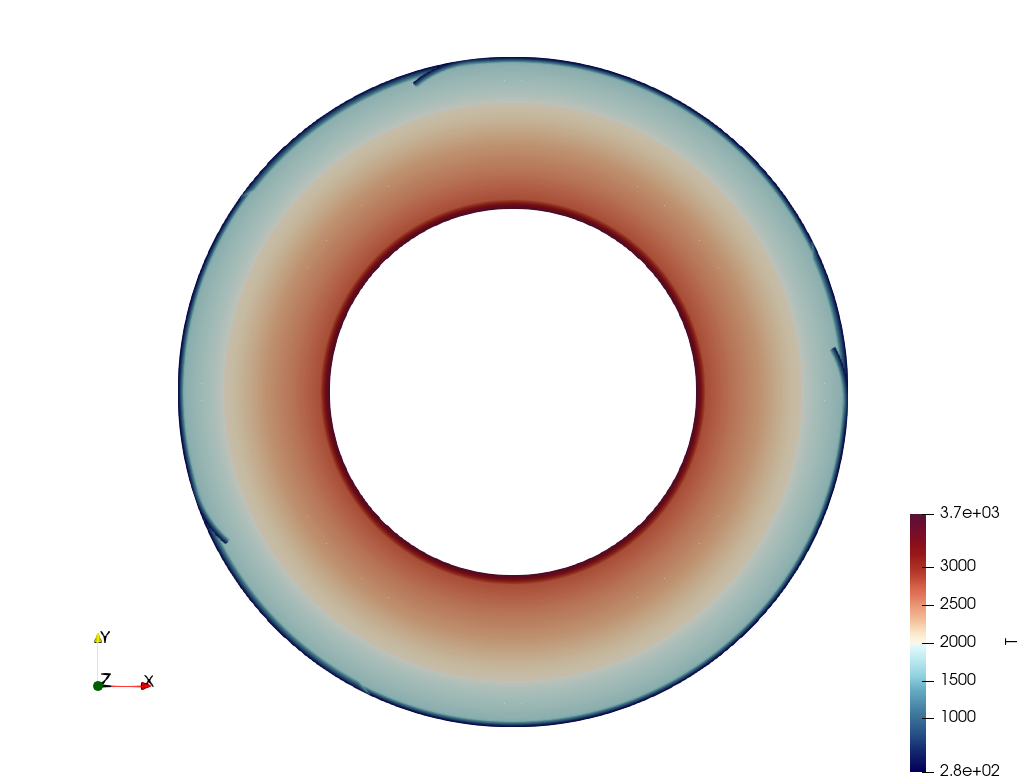
\includegraphics[width=0.3\textwidth]    {viz/plugins/maximum_horizontal_compressive_stress/temperature.png}  \hfill  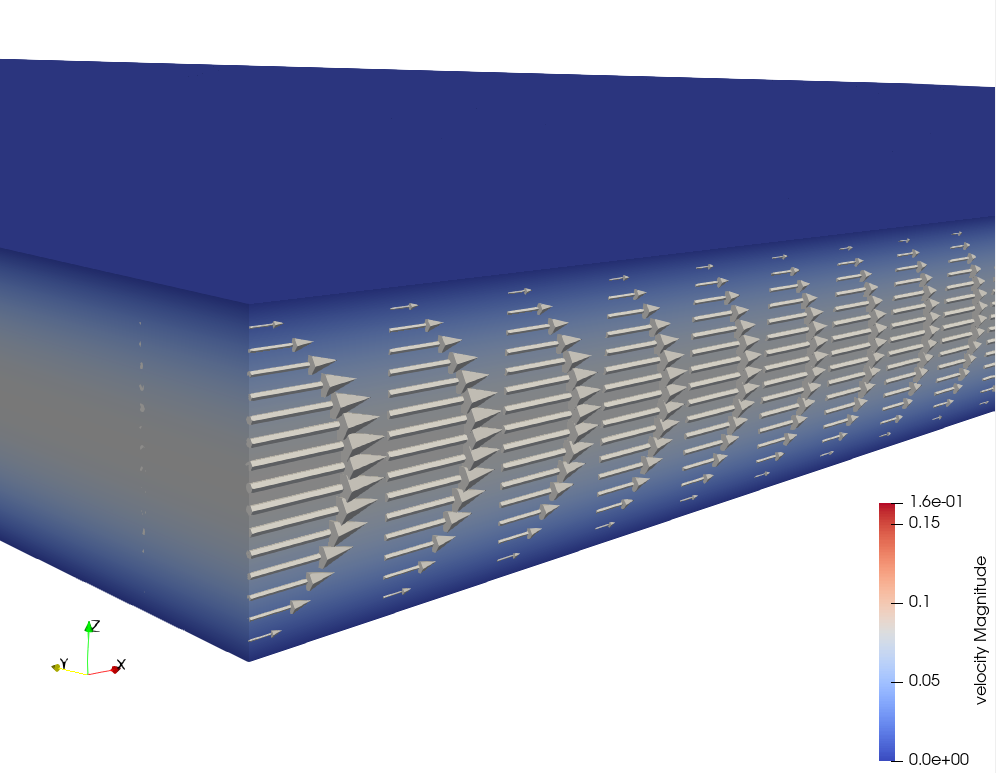
\includegraphics[width=0.3\textwidth]    {viz/plugins/maximum_horizontal_compressive_stress/velocity.png}  \hfill  \includegraphics[width=0.3\textwidth]    {viz/plugins/maximum_horizontal_compressive_stress/horizontal-stress.png}  \caption{\it Illustration of the `maximum horizontal     compressive stress' visualization plugin. The left     figure shows a ridge-like temperature anomaly. Together     with no-slip boundary along all six boundaries, this     results in two convection rolls (center). The maximal     horizontal compressive strength at the bottom center     of the domain is perpendicular to the ridge because     the flow comes together there from the left and right,     yielding a compressive force in left-right direction.     At the top of the model, the flow separates outward,     leading to a \textit{negative} compressive stress     in left-right direction; because there is no flow     in front-back direction, the compressive strength     in front-back direction is zero, making the along-ridge     direction the dominant one. At the center of the     convection rolls, both horizontal directions yield     the same stress; the plugin therefore chooses an     essentially arbitrary horizontal vector, but then     uses a zero magnitude given that the difference     between the maximal and minimal horizontal stress     is zero at these points.}  \label{fig:max-horizontal-compressive-stress}\end{figure}

Physical units: \si{\pascal}.

`melt fraction': A visualization output object that generates output for the melt fraction at the temperature and pressure of the current point. If the material model computes a melt fraction, this is the quantity that will be visualized. Otherwise, a specific parametrization for batch melting (as described in the following) will be used. It does not take into account latent heat. If there are no compositional fields, or no fields called 'pyroxenite',  this postprocessor will visualize the melt fraction of peridotite (calculated using the anhydrous model of Katz, 2003). If there is a compositional field called 'pyroxenite', the postprocessor assumes that this compositional field is the content of pyroxenite, and will visualize the melt fraction for a mixture of peridotite and pyroxenite (using the melting model of Sobolev, 2011 for pyroxenite). All the parameters that were used in these calculations can be changed in the input file, the most relevant maybe being the mass fraction of Cpx in peridotite in the Katz melting model (Mass fraction cpx), which right now has a default of 15\%. The corresponding $p$-$T$-diagrams can be generated by running the tests melt\_postprocessor\_peridotite and melt\_postprocessor\_pyroxenite.

Physical units: None.

`melt material properties': A visualization output object that generates output for melt related properties of the material model. Note that this postprocessor always outputs the compaction pressure, but can output a large range of additional properties, as selected in the ``List of properties'' parameter.

Physical units: Various, depending on what is being output.

`named additional outputs': Some material models can compute quantities other than those that typically appear in the equations that \aspect{} solves (such as the viscosity, density, etc). Examples of quantities material models may be able to compute are seismic velocities, or other quantities that can be derived from the state variables and the material coefficients such as the stress or stress anisotropies. These quantities are generically referred to as `named outputs' because they are given an explicit name different from the usual outputs of material models.

This visualization postprocessor outputs whatever quantities the material model can compute. What quantities these are is specific to the material model in use for a simulation, and for many models in fact does not contain any named outputs at all.

Physical units: Various, depending on what is being output.

`nonadiabatic pressure': A visualization output object that generates output for the non-adiabatic component of the pressure.

The variable that is outputted this way is computed by taking the pressure at each point and subtracting from it the adiabatic pressure computed at the beginning of the simulation. Because the adiabatic pressure is one way of defining a static pressure background field, what this visualization postprocessor therefore produces is \textit{one} way to compute a \textit{dynamic pressure}. There are, however, other ways as well, depending on the choice of the ``background pressure''.

Physical units: \si{\pascal}.

`nonadiabatic temperature': A visualization output object that generates output for the non-adiabatic component of the temperature.

Physical units: \si{\kelvin}.

`particle count': A visualization output object that generates output about the number of particles per cell.

Physical units: None.

`partition': A visualization output object that generates output for the parallel partition that every cell of the mesh is associated with.

Physical units: None.

`principal stress': A visualization output object that outputs the principal stress values and directions, i.e., the eigenvalues and eigenvectors of the stress tensor. The postprocessor can either operate on the full stress tensor or only on the deviatoric stress tensor, depending on what run-time parameters are set.

Physical units: \si{\pascal}.

`shear stress': A visualization output object that generates output for the 3 (in 2d) or 6 (in 3d) components of the shear stress tensor, i.e., for the components of the tensor $-2\eta\varepsilon(\mathbf u)$ in the incompressible case and $-2\eta\left[\varepsilon(\mathbf u)-\tfrac 13(\textrm{tr}\;\varepsilon(\mathbf u))\mathbf I\right]$ in the compressible case. If elasticity is used, the elastic contribution is being accounted for. The shear stress differs from the full stress tensor by the absence of the pressure. Note that the convention of positive compressive stress is followed.

Physical units: \si{\pascal}.

`spd factor': A visualization output object that generates output for the spd factor. The spd factor is a factor which scales a part of the Jacobian used for the Newton solver to make sure that the Jacobian remains positive definite.

Physical units: None.

`spherical velocity components': A visualization output object that outputs the polar coordinates components $v_r$ and $v_\phi$ of the velocity field in 2d and the spherical coordinates components $v_r$, $v_{\phi}$ and $v_{\theta}$ of the velocity field in 3d.

Physical units: $\frac{\text{m}}{\text{s}}$ or $\frac{\text{m}}{\text{year}}$, depending on settings in the input file.

`strain rate': A visualization output object that generates output for the norm of the strain rate, i.e., for the quantity $\sqrt{\varepsilon(\mathbf u):\varepsilon(\mathbf u)}$ in the incompressible case and $\sqrt{[\varepsilon(\mathbf u)-\tfrac 13(\textrm{tr}\;\varepsilon(\mathbf u))\mathbf I]:[\varepsilon(\mathbf u)-\tfrac 13(\textrm{tr}\;\varepsilon(\mathbf u))\mathbf I]}$ in the compressible case.

Physical units: \si{\per\second}.

`strain rate tensor': A visualization output object that generates output for the 4 (in 2d) or 9 (in 3d) components of the strain rate tensor, i.e., for the components of the tensor $\varepsilon(\mathbf u)$ in the incompressible case and $\varepsilon(\mathbf u)-\tfrac 13(\textrm{tr}\;\varepsilon(\mathbf u))\mathbf I$ in the compressible case.

Physical units: \si{\per\second}.

`stress': A visualization output object that generates output for the 3 (in 2d) or 6 (in 3d) components of the stress tensor, i.e., for the components of the tensor $-2\eta\varepsilon(\mathbf u)+pI$ in the incompressible case and $-2\eta\left[\varepsilon(\mathbf u)-\tfrac 13(\textrm{tr}\;\varepsilon(\mathbf u))\mathbf I\right]+pI$ in the compressible case. If elasticity is used, the elastic contribution is being accounted for. Note that the convention of positive compressive stress is followed.

Physical units: \si{\pascal}.

`stress second invariant': A visualization output object that outputs the second moment invariant of the deviatoric stress tensor.

Physical units: \si{\pascal}.

`surface dynamic topography': A visualization output object that generates output for the dynamic topography at the top and bottom of the model space. The approach to determine the dynamic topography requires us to compute the stress tensor and evaluate the component of it in the direction in which gravity acts. In other words, we compute $\sigma_{rr}={\hat g}^T(2 \eta \varepsilon(\mathbf u)-\frac 13 (\textrm{div}\;\mathbf u)I)\hat g - p_d$ where $\hat g = \mathbf g/\|\mathbf g\|$ is the direction of the gravity vector $\mathbf g$ and $p_d=p-p_a$ is the dynamic pressure computed by subtracting the adiabatic pressure $p_a$ from the total pressure $p$ computed as part of the Stokes solve. From this, the dynamic topography is computed using the formula $h=\frac{\sigma_{rr}}{(\mathbf g \cdot \mathbf n)  \rho}$ where $\rho$ is the density at the cell center. For the bottom surface we chose the convection that positive values are up (out) and negative values are in (down), analogous to the deformation of the upper surface. Note that this implementation takes the direction of gravity into account, which means that reversing the flow in backward advection calculations will not reverse the instantaneous topography because the reverse flow will be divided by the reverse surface gravity.

In contrast to the `dynamic topography' visualization postprocessor, this plugin really only evaluates the dynamic topography at faces of cells that are adjacent to `bottom' and `top' boundaries, and only outputs information on the surface of the domain, rather than padding the information with zeros in the interior of the domain.

Physical units: \si{\meter}.

`surface stress': A visualization output object that generates output on the surface of the domain for the 3 (in 2d) or 6 (in 3d) components of the stress tensor, i.e., for the components of the tensor $-2\eta\varepsilon(\mathbf u)+pI$ in the incompressible case and $-2\eta\left[\varepsilon(\mathbf u)-\tfrac 13(\textrm{tr}\;\varepsilon(\mathbf u))\mathbf I\right]+pI$ in the compressible case. If elasticity is included, its contribution is accounted for. Note that the convention of positive compressive stress is followed.

Physical units: \si{\pascal}.

`temperature anomaly': A visualization output postprocessor that outputs the temperature minus the depth-average of the temperature.The average temperature is calculated using the lateral averaging function from the ``depth average'' postprocessor and interpolated linearly between the layers specified through ``Number of depth slices''.

Physical units: \si{\kelvin}.

`vertical heat flux': A visualization output object that generates output for the heat flux in the vertical direction, which is the sum of the advective and the conductive heat flux, with the sign convention of positive flux upwards.

Physical units: \si{\watt\per\square\meter}.

`volume of fluid values': A visualization output object that outputs the volume fraction and optionally a level set field and the interface normal vectors of volume of fluid fields.

Physical units: None.

`volumetric strain rate': A visualization output object that generates output for the volumetric strain rate, i.e., for the quantity $\nabla\cdot\mathbf u = \textrm{div}\; \mathbf u = \textrm{trace}\; \varepsilon(\mathbf u)$. This should be zero (in some average sense) in incompressible convection models, but can be non-zero in compressible models and models with melt transport.

Physical units: \si{\per\second}.


{\it Possible values:} A comma-separated list of any of ISA rotation timescale, Vp anomaly, Vs anomaly, adiabat, artificial viscosity, artificial viscosity composition, boundary indicators, boundary strain rate residual, boundary velocity residual, compositional vector, depth, dynamic topography, error indicator, geoid, grain lag angle, gravity, heat flux map, heating, material properties, maximum horizontal compressive stress, melt fraction, melt material properties, named additional outputs, nonadiabatic pressure, nonadiabatic temperature, particle count, partition, principal stress, shear stress, spd factor, spherical velocity components, strain rate, strain rate tensor, stress, stress second invariant, surface dynamic topography, surface stress, temperature anomaly, vertical heat flux, volume of fluid values, volumetric strain rate, density, specific heat, thermal conductivity, thermal diffusivity, thermal expansivity, viscosity
\item {\it Parameter name:} {\tt Number of grouped files}
\phantomsection\label{parameters:Postprocess/Visualization/Number of grouped files}
\label{parameters:Postprocess/Visualization/Number_20of_20grouped_20files}


\index[prmindex]{Number of grouped files}
\index[prmindexfull]{Postprocess!Visualization!Number of grouped files}
{\it Value:} 16


{\it Default:} 16


{\it Description:} VTU file output supports grouping files from several CPUs into a given number of files using MPI I/O when writing on a parallel filesystem. Select 0 for no grouping. This will disable parallel file output and instead write one file per processor. A value of 1 will generate one big file containing the whole solution, while a larger value will create that many files (at most as many as there are MPI ranks).


{\it Possible values:} An integer $n$ such that $0\leq n \leq 2147483647$
\item {\it Parameter name:} {\tt Output format}
\phantomsection\label{parameters:Postprocess/Visualization/Output format}
\label{parameters:Postprocess/Visualization/Output_20format}


\index[prmindex]{Output format}
\index[prmindexfull]{Postprocess!Visualization!Output format}
{\it Value:} vtu


{\it Default:} vtu


{\it Description:} The file format to be used for graphical output. The list of possible output formats that can be given here is documented in the appendix of the manual where the current parameter is described.


{\it Possible values:} Any one of none, dx, ucd, gnuplot, povray, eps, gmv, tecplot, tecplot\_binary, vtk, vtu, hdf5, svg, deal.II intermediate
\item {\it Parameter name:} {\tt Output mesh displacement}
\phantomsection\label{parameters:Postprocess/Visualization/Output mesh displacement}
\label{parameters:Postprocess/Visualization/Output_20mesh_20displacement}


\index[prmindex]{Output mesh displacement}
\index[prmindexfull]{Postprocess!Visualization!Output mesh displacement}
{\it Value:} false


{\it Default:} false


{\it Description:} For computations with deforming meshes, ASPECT uses an Arbitrary-Lagrangian-Eulerian formulation to handle deforming the domain. The displacement vector from the reference configuration may be written as an output field by setting this parameter to true.


{\it Possible values:} A boolean value (true or false)
\item {\it Parameter name:} {\tt Output mesh velocity}
\phantomsection\label{parameters:Postprocess/Visualization/Output mesh velocity}
\label{parameters:Postprocess/Visualization/Output_20mesh_20velocity}


\index[prmindex]{Output mesh velocity}
\index[prmindexfull]{Postprocess!Visualization!Output mesh velocity}
{\it Value:} false


{\it Default:} false


{\it Description:} For computations with deforming meshes, ASPECT uses an Arbitrary-Lagrangian-Eulerian formulation to handle deforming the domain, so the mesh has its own velocity field.  This may be written as an output field by setting this parameter to true.


{\it Possible values:} A boolean value (true or false)
\item {\it Parameter name:} {\tt Output undeformed mesh}
\phantomsection\label{parameters:Postprocess/Visualization/Output undeformed mesh}
\label{parameters:Postprocess/Visualization/Output_20undeformed_20mesh}


\index[prmindex]{Output undeformed mesh}
\index[prmindexfull]{Postprocess!Visualization!Output undeformed mesh}
{\it Value:} false


{\it Default:} false


{\it Description:} For computations with deforming meshes, ASPECT uses an Arbitrary-Lagrangian-Eulerian formulation to handle deforming the domain. By default, we output the deformed mesh. If this setting is set to true, the mesh will be written in the reference state without deformation instead. If you output the mesh displacement, you can obtain the deformed mesh by using the 'warp by vector' ParaView filter.


{\it Possible values:} A boolean value (true or false)
\item {\it Parameter name:} {\tt Point-wise stress and strain}
\phantomsection\label{parameters:Postprocess/Visualization/Point_2dwise stress and strain}
\label{parameters:Postprocess/Visualization/Point_2dwise_20stress_20and_20strain}


\index[prmindex]{Point-wise stress and strain}
\index[prmindexfull]{Postprocess!Visualization!Point-wise stress and strain}
{\it Value:} false


{\it Default:} false


{\it Description:} If set to true, quantities related to stress and strain are computed in each vertex. Otherwise, an average per cell is computed.


{\it Possible values:} A boolean value (true or false)
\item {\it Parameter name:} {\tt Temporary output location}
\phantomsection\label{parameters:Postprocess/Visualization/Temporary output location}
\label{parameters:Postprocess/Visualization/Temporary_20output_20location}


\index[prmindex]{Temporary output location}
\index[prmindexfull]{Postprocess!Visualization!Temporary output location}
{\it Value:} 


{\it Default:} 


{\it Description:} On large clusters it can be advantageous to first write the output to a temporary file on a local file system and later move this file to a network file system. If this variable is set to a non-empty string it will be interpreted as a temporary storage location.


{\it Possible values:} Any string
\item {\it Parameter name:} {\tt Time between graphical output}
\phantomsection\label{parameters:Postprocess/Visualization/Time between graphical output}
\label{parameters:Postprocess/Visualization/Time_20between_20graphical_20output}


\index[prmindex]{Time between graphical output}
\index[prmindexfull]{Postprocess!Visualization!Time between graphical output}
{\it Value:} 1e8


{\it Default:} 1e8


{\it Description:} The time interval between each generation of graphical output files. A value of zero indicates that output should be generated in each time step. Units: years if the 'Use years in output instead of seconds' parameter is set; seconds otherwise.


{\it Possible values:} A floating point number $v$ such that $0 \leq v \leq \text{MAX\_DOUBLE}$
\item {\it Parameter name:} {\tt Time steps between graphical output}
\phantomsection\label{parameters:Postprocess/Visualization/Time steps between graphical output}
\label{parameters:Postprocess/Visualization/Time_20steps_20between_20graphical_20output}


\index[prmindex]{Time steps between graphical output}
\index[prmindexfull]{Postprocess!Visualization!Time steps between graphical output}
{\it Value:} 2147483647


{\it Default:} 2147483647


{\it Description:} The maximum number of time steps between each generation of graphical output files.


{\it Possible values:} An integer $n$ such that $0\leq n \leq 2147483647$
\item {\it Parameter name:} {\tt Write higher order output}
\phantomsection\label{parameters:Postprocess/Visualization/Write higher order output}
\label{parameters:Postprocess/Visualization/Write_20higher_20order_20output}


\index[prmindex]{Write higher order output}
\index[prmindexfull]{Postprocess!Visualization!Write higher order output}
{\it Value:} false


{\it Default:} false


{\it Description:} deal.II offers the possibility to write vtu files with higher order representations of the output data. This means each cell will correctly show the higher order representation of the output data instead of the linear interpolation between vertices that ParaView and VisIt usually show. Note that activating this option is safe and recommended, but requires that (i) ``Output format'' is set to ``vtu'', (ii) ``Interpolate output'' is set to true, (iii) you use a sufficiently new version of Paraview or VisIt to read the files (Paraview version 5.5 or newer, and VisIt version to be determined), and (iv) you use deal.II version 9.1.0 or newer. 
The effect of using this option can be seen in the following picture:

\begin{center}  \includegraphics[width=0.5\textwidth]{viz/parameters/higher-order-output}\end{center}The top figure shows the plain output without interpolation or higher order output. The middle figure shows output that was interpolated as discussed for the ``Interpolate output'' option. The bottom panel shows higher order output that achieves better accuracy than the interpolated output at a lower memory cost.


{\it Possible values:} A boolean value (true or false)
\item {\it Parameter name:} {\tt Write in background thread}
\phantomsection\label{parameters:Postprocess/Visualization/Write in background thread}
\label{parameters:Postprocess/Visualization/Write_20in_20background_20thread}


\index[prmindex]{Write in background thread}
\index[prmindexfull]{Postprocess!Visualization!Write in background thread}
{\it Value:} false


{\it Default:} false


{\it Description:} File operations can potentially take a long time, blocking the progress of the rest of the model run. Setting this variable to `true' moves this process into a background thread, while the rest of the model continues.


{\it Possible values:} A boolean value (true or false)
\end{itemize}



\subsection{Parameters in section \tt Postprocess/Visualization/Artificial viscosity composition}
\label{parameters:Postprocess/Visualization/Artificial_20viscosity_20composition}

\begin{itemize}
\item {\it Parameter name:} {\tt Name of compositional field}
\phantomsection\label{parameters:Postprocess/Visualization/Artificial viscosity composition/Name of compositional field}
\label{parameters:Postprocess/Visualization/Artificial_20viscosity_20composition/Name_20of_20compositional_20field}


\index[prmindex]{Name of compositional field}
\index[prmindexfull]{Postprocess!Visualization!Artificial viscosity composition/Name of compositional field}
{\it Value:} 


{\it Default:} 


{\it Description:} The name of the compositional field whose output should be visualized. 


{\it Possible values:} Any string
\end{itemize}

\subsection{Parameters in section \tt Postprocess/Visualization/Compositional fields as vectors}
\label{parameters:Postprocess/Visualization/Compositional_20fields_20as_20vectors}

\begin{itemize}
\item {\it Parameter name:} {\tt Names of fields}
\phantomsection\label{parameters:Postprocess/Visualization/Compositional fields as vectors/Names of fields}
\label{parameters:Postprocess/Visualization/Compositional_20fields_20as_20vectors/Names_20of_20fields}


\index[prmindex]{Names of fields}
\index[prmindexfull]{Postprocess!Visualization!Compositional fields as vectors/Names of fields}
{\it Value:} 


{\it Default:} 


{\it Description:} A list of sets of compositional fields which should be output as vectors. Sets are separated from each other by semicolons and vector components within each set are separated by commas (e.g. $vec1_x$, $vec1_y$ ; $vec2_x$, $vec2_y$) where each name must be a defined named compositional field. If only one name is given in a set, it is interpreted as the first in a sequence of dim consecutive compositional fields.


{\it Possible values:} Any string
\item {\it Parameter name:} {\tt Names of vectors}
\phantomsection\label{parameters:Postprocess/Visualization/Compositional fields as vectors/Names of vectors}
\label{parameters:Postprocess/Visualization/Compositional_20fields_20as_20vectors/Names_20of_20vectors}


\index[prmindex]{Names of vectors}
\index[prmindexfull]{Postprocess!Visualization!Compositional fields as vectors/Names of vectors}
{\it Value:} 


{\it Default:} 


{\it Description:} Names of vectors as they will appear in the output.


{\it Possible values:} A list of 0 to 4294967295 elements where each element is [Any string]
\end{itemize}

\subsection{Parameters in section \tt Postprocess/Visualization/Heat flux map}
\label{parameters:Postprocess/Visualization/Heat_20flux_20map}

\begin{itemize}
\item {\it Parameter name:} {\tt Output point wise heat flux}
\phantomsection\label{parameters:Postprocess/Visualization/Heat flux map/Output point wise heat flux}
\label{parameters:Postprocess/Visualization/Heat_20flux_20map/Output_20point_20wise_20heat_20flux}


\index[prmindex]{Output point wise heat flux}
\index[prmindexfull]{Postprocess!Visualization!Heat flux map/Output point wise heat flux}
{\it Value:} false


{\it Default:} false


{\it Description:} A boolean flag that controls whether to output the heat flux map as a point wise value, or as a cell-wise averaged value. The point wise output is more accurate, but it currently omits prescribed heat flux values at boundaries and advective heat flux that is caused by velocities non-tangential to boundaries. If you do not use these two features it is recommended to switch this setting on to benefit from the increased output resolution.


{\it Possible values:} A boolean value (true or false)
\end{itemize}

\subsection{Parameters in section \tt Postprocess/Visualization/Material properties}
\label{parameters:Postprocess/Visualization/Material_20properties}

\begin{itemize}
\item {\it Parameter name:} {\tt List of material properties}
\phantomsection\label{parameters:Postprocess/Visualization/Material properties/List of material properties}
\label{parameters:Postprocess/Visualization/Material_20properties/List_20of_20material_20properties}


\index[prmindex]{List of material properties}
\index[prmindexfull]{Postprocess!Visualization!Material properties/List of material properties}
{\it Value:} density,thermal expansivity,specific heat,viscosity


{\it Default:} density,thermal expansivity,specific heat,viscosity


{\it Description:} A comma separated list of material properties that should be written whenever writing graphical output. By default, the material properties will always contain the density, thermal expansivity, specific heat and viscosity. The following material properties are available:

viscosity|density|thermal expansivity|specific heat|thermal conductivity|thermal diffusivity|compressibility|entropy derivative temperature|entropy derivative pressure|reaction terms|melt fraction


{\it Possible values:} A comma-separated list of any of viscosity, density, thermal expansivity, specific heat, thermal conductivity, thermal diffusivity, compressibility, entropy derivative temperature, entropy derivative pressure, reaction terms, melt fraction
\end{itemize}

\subsection{Parameters in section \tt Postprocess/Visualization/Melt fraction}
\label{parameters:Postprocess/Visualization/Melt_20fraction}

\begin{itemize}
\item {\it Parameter name:} {\tt A1}
\phantomsection\label{parameters:Postprocess/Visualization/Melt fraction/A1}
\label{parameters:Postprocess/Visualization/Melt_20fraction/A1}


\index[prmindex]{A1}
\index[prmindexfull]{Postprocess!Visualization!Melt fraction/A1}
{\it Value:} 1085.7


{\it Default:} 1085.7


{\it Description:} Constant parameter in the quadratic function that approximates the solidus of peridotite. Units: \si{\degreeCelsius}.


{\it Possible values:} A floating point number $v$ such that $-\text{MAX\_DOUBLE} \leq v \leq \text{MAX\_DOUBLE}$
\item {\it Parameter name:} {\tt A2}
\phantomsection\label{parameters:Postprocess/Visualization/Melt fraction/A2}
\label{parameters:Postprocess/Visualization/Melt_20fraction/A2}


\index[prmindex]{A2}
\index[prmindexfull]{Postprocess!Visualization!Melt fraction/A2}
{\it Value:} 1.329e-7


{\it Default:} 1.329e-7


{\it Description:} Prefactor of the linear pressure term in the quadratic function that approximates the solidus of peridotite. \si{\degreeCelsius\per\pascal}.


{\it Possible values:} A floating point number $v$ such that $-\text{MAX\_DOUBLE} \leq v \leq \text{MAX\_DOUBLE}$
\item {\it Parameter name:} {\tt A3}
\phantomsection\label{parameters:Postprocess/Visualization/Melt fraction/A3}
\label{parameters:Postprocess/Visualization/Melt_20fraction/A3}


\index[prmindex]{A3}
\index[prmindexfull]{Postprocess!Visualization!Melt fraction/A3}
{\it Value:} -5.1e-18


{\it Default:} -5.1e-18


{\it Description:} Prefactor of the quadratic pressure term in the quadratic function that approximates the solidus of peridotite. \si{\degreeCelsius\per\pascal\squared}.


{\it Possible values:} A floating point number $v$ such that $-\text{MAX\_DOUBLE} \leq v \leq \text{MAX\_DOUBLE}$
\item {\it Parameter name:} {\tt B1}
\phantomsection\label{parameters:Postprocess/Visualization/Melt fraction/B1}
\label{parameters:Postprocess/Visualization/Melt_20fraction/B1}


\index[prmindex]{B1}
\index[prmindexfull]{Postprocess!Visualization!Melt fraction/B1}
{\it Value:} 1475.0


{\it Default:} 1475.0


{\it Description:} Constant parameter in the quadratic function that approximates the lherzolite liquidus used for calculating the fraction of peridotite-derived melt. Units: \si{\degreeCelsius}.


{\it Possible values:} A floating point number $v$ such that $-\text{MAX\_DOUBLE} \leq v \leq \text{MAX\_DOUBLE}$
\item {\it Parameter name:} {\tt B2}
\phantomsection\label{parameters:Postprocess/Visualization/Melt fraction/B2}
\label{parameters:Postprocess/Visualization/Melt_20fraction/B2}


\index[prmindex]{B2}
\index[prmindexfull]{Postprocess!Visualization!Melt fraction/B2}
{\it Value:} 8.0e-8


{\it Default:} 8.0e-8


{\it Description:} Prefactor of the linear pressure term in the quadratic function that approximates the  lherzolite liquidus used for calculating the fraction of peridotite-derived melt. \si{\degreeCelsius\per\pascal}.


{\it Possible values:} A floating point number $v$ such that $-\text{MAX\_DOUBLE} \leq v \leq \text{MAX\_DOUBLE}$
\item {\it Parameter name:} {\tt B3}
\phantomsection\label{parameters:Postprocess/Visualization/Melt fraction/B3}
\label{parameters:Postprocess/Visualization/Melt_20fraction/B3}


\index[prmindex]{B3}
\index[prmindexfull]{Postprocess!Visualization!Melt fraction/B3}
{\it Value:} -3.2e-18


{\it Default:} -3.2e-18


{\it Description:} Prefactor of the quadratic pressure term in the quadratic function that approximates the  lherzolite liquidus used for calculating the fraction of peridotite-derived melt. \si{\degreeCelsius\per\pascal\squared}.


{\it Possible values:} A floating point number $v$ such that $-\text{MAX\_DOUBLE} \leq v \leq \text{MAX\_DOUBLE}$
\item {\it Parameter name:} {\tt C1}
\phantomsection\label{parameters:Postprocess/Visualization/Melt fraction/C1}
\label{parameters:Postprocess/Visualization/Melt_20fraction/C1}


\index[prmindex]{C1}
\index[prmindexfull]{Postprocess!Visualization!Melt fraction/C1}
{\it Value:} 1780.0


{\it Default:} 1780.0


{\it Description:} Constant parameter in the quadratic function that approximates the liquidus of peridotite. Units: \si{\degreeCelsius}.


{\it Possible values:} A floating point number $v$ such that $-\text{MAX\_DOUBLE} \leq v \leq \text{MAX\_DOUBLE}$
\item {\it Parameter name:} {\tt C2}
\phantomsection\label{parameters:Postprocess/Visualization/Melt fraction/C2}
\label{parameters:Postprocess/Visualization/Melt_20fraction/C2}


\index[prmindex]{C2}
\index[prmindexfull]{Postprocess!Visualization!Melt fraction/C2}
{\it Value:} 4.50e-8


{\it Default:} 4.50e-8


{\it Description:} Prefactor of the linear pressure term in the quadratic function that approximates the liquidus of peridotite. \si{\degreeCelsius\per\pascal}.


{\it Possible values:} A floating point number $v$ such that $-\text{MAX\_DOUBLE} \leq v \leq \text{MAX\_DOUBLE}$
\item {\it Parameter name:} {\tt C3}
\phantomsection\label{parameters:Postprocess/Visualization/Melt fraction/C3}
\label{parameters:Postprocess/Visualization/Melt_20fraction/C3}


\index[prmindex]{C3}
\index[prmindexfull]{Postprocess!Visualization!Melt fraction/C3}
{\it Value:} -2.0e-18


{\it Default:} -2.0e-18


{\it Description:} Prefactor of the quadratic pressure term in the quadratic function that approximates the liquidus of peridotite. \si{\degreeCelsius\per\pascal\squared}.


{\it Possible values:} A floating point number $v$ such that $-\text{MAX\_DOUBLE} \leq v \leq \text{MAX\_DOUBLE}$
\item {\it Parameter name:} {\tt D1}
\phantomsection\label{parameters:Postprocess/Visualization/Melt fraction/D1}
\label{parameters:Postprocess/Visualization/Melt_20fraction/D1}


\index[prmindex]{D1}
\index[prmindexfull]{Postprocess!Visualization!Melt fraction/D1}
{\it Value:} 976.0


{\it Default:} 976.0


{\it Description:} Constant parameter in the quadratic function that approximates the solidus of pyroxenite. Units: \si{\degreeCelsius}.


{\it Possible values:} A floating point number $v$ such that $-\text{MAX\_DOUBLE} \leq v \leq \text{MAX\_DOUBLE}$
\item {\it Parameter name:} {\tt D2}
\phantomsection\label{parameters:Postprocess/Visualization/Melt fraction/D2}
\label{parameters:Postprocess/Visualization/Melt_20fraction/D2}


\index[prmindex]{D2}
\index[prmindexfull]{Postprocess!Visualization!Melt fraction/D2}
{\it Value:} 1.329e-7


{\it Default:} 1.329e-7


{\it Description:} Prefactor of the linear pressure term in the quadratic function that approximates the solidus of pyroxenite. Note that this factor is different from the value given in Sobolev, 2011, because they use the potential temperature whereas we use the absolute temperature. \si{\degreeCelsius\per\pascal}.


{\it Possible values:} A floating point number $v$ such that $-\text{MAX\_DOUBLE} \leq v \leq \text{MAX\_DOUBLE}$
\item {\it Parameter name:} {\tt D3}
\phantomsection\label{parameters:Postprocess/Visualization/Melt fraction/D3}
\label{parameters:Postprocess/Visualization/Melt_20fraction/D3}


\index[prmindex]{D3}
\index[prmindexfull]{Postprocess!Visualization!Melt fraction/D3}
{\it Value:} -5.1e-18


{\it Default:} -5.1e-18


{\it Description:} Prefactor of the quadratic pressure term in the quadratic function that approximates the solidus of pyroxenite. \si{\degreeCelsius\per\pascal\squared}.


{\it Possible values:} A floating point number $v$ such that $-\text{MAX\_DOUBLE} \leq v \leq \text{MAX\_DOUBLE}$
\item {\it Parameter name:} {\tt E1}
\phantomsection\label{parameters:Postprocess/Visualization/Melt fraction/E1}
\label{parameters:Postprocess/Visualization/Melt_20fraction/E1}


\index[prmindex]{E1}
\index[prmindexfull]{Postprocess!Visualization!Melt fraction/E1}
{\it Value:} 663.8


{\it Default:} 663.8


{\it Description:} Prefactor of the linear depletion term in the quadratic function that approximates the melt fraction of pyroxenite. \si{\degreeCelsius\per\pascal}.


{\it Possible values:} A floating point number $v$ such that $-\text{MAX\_DOUBLE} \leq v \leq \text{MAX\_DOUBLE}$
\item {\it Parameter name:} {\tt E2}
\phantomsection\label{parameters:Postprocess/Visualization/Melt fraction/E2}
\label{parameters:Postprocess/Visualization/Melt_20fraction/E2}


\index[prmindex]{E2}
\index[prmindexfull]{Postprocess!Visualization!Melt fraction/E2}
{\it Value:} -611.4


{\it Default:} -611.4


{\it Description:} Prefactor of the quadratic depletion term in the quadratic function that approximates the melt fraction of pyroxenite. \si{\degreeCelsius\per\pascal\squared}.


{\it Possible values:} A floating point number $v$ such that $-\text{MAX\_DOUBLE} \leq v \leq \text{MAX\_DOUBLE}$
\item {\it Parameter name:} {\tt Mass fraction cpx}
\phantomsection\label{parameters:Postprocess/Visualization/Melt fraction/Mass fraction cpx}
\label{parameters:Postprocess/Visualization/Melt_20fraction/Mass_20fraction_20cpx}


\index[prmindex]{Mass fraction cpx}
\index[prmindexfull]{Postprocess!Visualization!Melt fraction/Mass fraction cpx}
{\it Value:} 0.15


{\it Default:} 0.15


{\it Description:} Mass fraction of clinopyroxene in the peridotite to be molten. Units: non-dimensional.


{\it Possible values:} A floating point number $v$ such that $-\text{MAX\_DOUBLE} \leq v \leq \text{MAX\_DOUBLE}$
\item {\it Parameter name:} {\tt beta}
\phantomsection\label{parameters:Postprocess/Visualization/Melt fraction/beta}
\label{parameters:Postprocess/Visualization/Melt_20fraction/beta}


\index[prmindex]{beta}
\index[prmindexfull]{Postprocess!Visualization!Melt fraction/beta}
{\it Value:} 1.5


{\it Default:} 1.5


{\it Description:} Exponent of the melting temperature in the melt fraction calculation. Units: non-dimensional.


{\it Possible values:} A floating point number $v$ such that $-\text{MAX\_DOUBLE} \leq v \leq \text{MAX\_DOUBLE}$
\item {\it Parameter name:} {\tt r1}
\phantomsection\label{parameters:Postprocess/Visualization/Melt fraction/r1}
\label{parameters:Postprocess/Visualization/Melt_20fraction/r1}


\index[prmindex]{r1}
\index[prmindexfull]{Postprocess!Visualization!Melt fraction/r1}
{\it Value:} 0.5


{\it Default:} 0.5


{\it Description:} Constant in the linear function that approximates the clinopyroxene reaction coefficient. Units: non-dimensional.


{\it Possible values:} A floating point number $v$ such that $-\text{MAX\_DOUBLE} \leq v \leq \text{MAX\_DOUBLE}$
\item {\it Parameter name:} {\tt r2}
\phantomsection\label{parameters:Postprocess/Visualization/Melt fraction/r2}
\label{parameters:Postprocess/Visualization/Melt_20fraction/r2}


\index[prmindex]{r2}
\index[prmindexfull]{Postprocess!Visualization!Melt fraction/r2}
{\it Value:} 8e-11


{\it Default:} 8e-11


{\it Description:} Prefactor of the linear pressure term in the linear function that approximates the clinopyroxene reaction coefficient. Units: \si{\per\pascal}.


{\it Possible values:} A floating point number $v$ such that $-\text{MAX\_DOUBLE} \leq v \leq \text{MAX\_DOUBLE}$
\end{itemize}

\subsection{Parameters in section \tt Postprocess/Visualization/Melt material properties}
\label{parameters:Postprocess/Visualization/Melt_20material_20properties}

\begin{itemize}
\item {\it Parameter name:} {\tt List of properties}
\phantomsection\label{parameters:Postprocess/Visualization/Melt material properties/List of properties}
\label{parameters:Postprocess/Visualization/Melt_20material_20properties/List_20of_20properties}


\index[prmindex]{List of properties}
\index[prmindexfull]{Postprocess!Visualization!Melt material properties/List of properties}
{\it Value:} compaction viscosity,permeability


{\it Default:} compaction viscosity,permeability


{\it Description:} A comma separated list of melt properties that should be written whenever writing graphical output. The following material properties are available:

compaction viscosity|fluid viscosity|permeability|fluid density|fluid density gradient|is melt cell|darcy coefficient|darcy coefficient no cutoff|compaction length


{\it Possible values:} A comma-separated list of any of compaction viscosity, fluid viscosity, permeability, fluid density, fluid density gradient, is melt cell, darcy coefficient, darcy coefficient no cutoff, compaction length
\end{itemize}

\subsection{Parameters in section \tt Postprocess/Visualization/Principal stress}
\label{parameters:Postprocess/Visualization/Principal_20stress}

\begin{itemize}
\item {\it Parameter name:} {\tt Use deviatoric stress}
\phantomsection\label{parameters:Postprocess/Visualization/Principal stress/Use deviatoric stress}
\label{parameters:Postprocess/Visualization/Principal_20stress/Use_20deviatoric_20stress}


\index[prmindex]{Use deviatoric stress}
\index[prmindexfull]{Postprocess!Visualization!Principal stress/Use deviatoric stress}
{\it Value:} false


{\it Default:} false


{\it Description:} Whether to use the deviatoric stress tensor instead of the full stress tensor to compute principal stress directions and values.


{\it Possible values:} A boolean value (true or false)
\end{itemize}

\subsection{Parameters in section \tt Postprocess/Visualization/Temperature anomaly}
\label{parameters:Postprocess/Visualization/Temperature_20anomaly}

\begin{itemize}
\item {\it Parameter name:} {\tt Number of depth slices}
\phantomsection\label{parameters:Postprocess/Visualization/Temperature anomaly/Number of depth slices}
\label{parameters:Postprocess/Visualization/Temperature_20anomaly/Number_20of_20depth_20slices}


\index[prmindex]{Number of depth slices}
\index[prmindexfull]{Postprocess!Visualization!Temperature anomaly/Number of depth slices}
{\it Value:} 20


{\it Default:} 20


{\it Description:} Number of depth slices used to define average temperature.


{\it Possible values:} An integer $n$ such that $1\leq n \leq 2147483647$
\item {\it Parameter name:} {\tt Use maximal temperature for bottom}
\phantomsection\label{parameters:Postprocess/Visualization/Temperature anomaly/Use maximal temperature for bottom}
\label{parameters:Postprocess/Visualization/Temperature_20anomaly/Use_20maximal_20temperature_20for_20bottom}


\index[prmindex]{Use maximal temperature for bottom}
\index[prmindexfull]{Postprocess!Visualization!Temperature anomaly/Use maximal temperature for bottom}
{\it Value:} true


{\it Default:} true


{\it Description:} If true, use the specified boundary temperatures as average temperatures at the surface. If false, extrapolate the temperature gradient between the first and second cells to the surface. This option will only work for models with a fixed surface temperature. 


{\it Possible values:} A boolean value (true or false)
\item {\it Parameter name:} {\tt Use minimal temperature for surface}
\phantomsection\label{parameters:Postprocess/Visualization/Temperature anomaly/Use minimal temperature for surface}
\label{parameters:Postprocess/Visualization/Temperature_20anomaly/Use_20minimal_20temperature_20for_20surface}


\index[prmindex]{Use minimal temperature for surface}
\index[prmindexfull]{Postprocess!Visualization!Temperature anomaly/Use minimal temperature for surface}
{\it Value:} true


{\it Default:} true


{\it Description:} Whether to use the minimal specified boundary temperature as the bottom boundary temperature. This option will only work for models with a fixed bottom boundary temperature. 


{\it Possible values:} A boolean value (true or false)
\end{itemize}

\subsection{Parameters in section \tt Postprocess/Visualization/Volume of Fluid}
\label{parameters:Postprocess/Visualization/Volume_20of_20Fluid}

\begin{itemize}
\item {\it Parameter name:} {\tt Output interface normals}
\phantomsection\label{parameters:Postprocess/Visualization/Volume of Fluid/Output interface normals}
\label{parameters:Postprocess/Visualization/Volume_20of_20Fluid/Output_20interface_20normals}


\index[prmindex]{Output interface normals}
\index[prmindexfull]{Postprocess!Visualization!Volume of Fluid/Output interface normals}
{\it Value:} false


{\it Default:} false


{\it Description:} Include the internal data for the interface normal on the unit cells.


{\it Possible values:} A boolean value (true or false)
\item {\it Parameter name:} {\tt Output interface reconstruction contour}
\phantomsection\label{parameters:Postprocess/Visualization/Volume of Fluid/Output interface reconstruction contour}
\label{parameters:Postprocess/Visualization/Volume_20of_20Fluid/Output_20interface_20reconstruction_20contour}


\index[prmindex]{Output interface reconstruction contour}
\index[prmindexfull]{Postprocess!Visualization!Volume of Fluid/Output interface reconstruction contour}
{\it Value:} false


{\it Default:} false


{\it Description:} Include fields defined such that the 0 contour is the fluid interface.


{\it Possible values:} A boolean value (true or false)
\end{itemize}

\subsection{Parameters in section \tt Postprocess/Visualization/Vp anomaly}
\label{parameters:Postprocess/Visualization/Vp_20anomaly}

\begin{itemize}
\item {\it Parameter name:} {\tt Average velocity scheme}
\phantomsection\label{parameters:Postprocess/Visualization/Vp anomaly/Average velocity scheme}
\label{parameters:Postprocess/Visualization/Vp_20anomaly/Average_20velocity_20scheme}


\index[prmindex]{Average velocity scheme}
\index[prmindexfull]{Postprocess!Visualization!Vp anomaly/Average velocity scheme}
{\it Value:} reference profile


{\it Default:} reference profile


{\it Description:} Scheme to compute the average velocity-depth profile. The reference profile option evaluates the conditions along the reference adiabat according to the material model. The lateral average option instead calculates a lateral average from subdivision of the mesh. The lateral average option may produce spurious results where there are sharp velocity changes.


{\it Possible values:} Any one of reference profile, lateral average
\item {\it Parameter name:} {\tt Number of depth slices}
\phantomsection\label{parameters:Postprocess/Visualization/Vp anomaly/Number of depth slices}
\label{parameters:Postprocess/Visualization/Vp_20anomaly/Number_20of_20depth_20slices}


\index[prmindex]{Number of depth slices}
\index[prmindexfull]{Postprocess!Visualization!Vp anomaly/Number of depth slices}
{\it Value:} 50


{\it Default:} 50


{\it Description:} Number of depth slices used to define average seismic compressional wave velocities from which anomalies are calculated. Units: non-dimensional.


{\it Possible values:} An integer $n$ such that $1\leq n \leq 2147483647$
\end{itemize}

\subsection{Parameters in section \tt Postprocess/Visualization/Vs anomaly}
\label{parameters:Postprocess/Visualization/Vs_20anomaly}

\begin{itemize}
\item {\it Parameter name:} {\tt Average velocity scheme}
\phantomsection\label{parameters:Postprocess/Visualization/Vs anomaly/Average velocity scheme}
\label{parameters:Postprocess/Visualization/Vs_20anomaly/Average_20velocity_20scheme}


\index[prmindex]{Average velocity scheme}
\index[prmindexfull]{Postprocess!Visualization!Vs anomaly/Average velocity scheme}
{\it Value:} reference profile


{\it Default:} reference profile


{\it Description:} Scheme to compute the average velocity-depth profile. The reference profile option evaluates the conditions along the reference adiabat according to the material model. The lateral average option instead calculates a lateral average from subdivision of the mesh. The lateral average option may produce spurious results where there are sharp velocity changes.


{\it Possible values:} Any one of reference profile, lateral average
\item {\it Parameter name:} {\tt Number of depth slices}
\phantomsection\label{parameters:Postprocess/Visualization/Vs anomaly/Number of depth slices}
\label{parameters:Postprocess/Visualization/Vs_20anomaly/Number_20of_20depth_20slices}


\index[prmindex]{Number of depth slices}
\index[prmindexfull]{Postprocess!Visualization!Vs anomaly/Number of depth slices}
{\it Value:} 50


{\it Default:} 50


{\it Description:} Number of depth slices used to define average seismic shear wave velocities from which anomalies are calculated. Units: non-dimensional.


{\it Possible values:} An integer $n$ such that $1\leq n \leq 2147483647$
\end{itemize}

\subsection{Parameters in section \tt Prescribed Stokes solution}
\label{parameters:Prescribed_20Stokes_20solution}

\begin{itemize}
\item {\it Parameter name:} {\tt Model name}
\phantomsection\label{parameters:Prescribed Stokes solution/Model name}
\label{parameters:Prescribed_20Stokes_20solution/Model_20name}


\index[prmindex]{Model name}
\index[prmindexfull]{Prescribed Stokes solution!Model name}
{\it Value:} unspecified


{\it Default:} unspecified


{\it Description:} Select one of the following models:

`ascii data': Implementation of a model in which the velocity is derived from files containing data in ascii format. Note the required format of the input data: The first lines may contain any number of comments if they begin with `\#', but one of these lines needs to contain the number of grid points in each dimension as for example `\# POINTS: 3 3'. The order of the data columns has to be `x', `y', `v${}_x$' , `v${}_y$' in a 2d model and  `x', `y', `z', `v${}_x$' , `v${}_y$' , `v${}_z$' in a 3d model. Note that the data in the input files need to be sorted in a specific order: the first coordinate needs to ascend first, followed by the second and the third at last in order to assign the correct data to the prescribed coordinates. If you use a spherical model, then the data will still be handled as Cartesian, however the assumed grid changes. `x' will be replaced by the radial distance of the point to the bottom of the model, `y' by the azimuth angle and `z' by the polar angle measured positive from the north pole. The grid will be assumed to be a latitude-longitude grid. Note that the order of spherical coordinates is `r', `phi', `theta' and not `r', `theta', `phi', since this allows for dimension independent expressions.

`circle': This value describes a vector field that rotates around the z-axis with constant angular velocity (i.e., with a velocity that increases with distance from the axis). The pressure is set to zero.

`function': This plugin allows to prescribe the Stokes solution for the velocity and pressure field in terms of an explicit formula. The format of these functions follows the syntax understood by the muparser library, see Section~\ref{sec:muparser-format}.


{\it Possible values:} Any one of ascii data, circle, function, unspecified
\end{itemize}



\subsection{Parameters in section \tt Prescribed Stokes solution/Ascii data model}
\label{parameters:Prescribed_20Stokes_20solution/Ascii_20data_20model}

\begin{itemize}
\item {\it Parameter name:} {\tt Data directory}
\phantomsection\label{parameters:Prescribed Stokes solution/Ascii data model/Data directory}
\label{parameters:Prescribed_20Stokes_20solution/Ascii_20data_20model/Data_20directory}


\index[prmindex]{Data directory}
\index[prmindexfull]{Prescribed Stokes solution!Ascii data model!Data directory}
{\it Value:} \$ASPECT\_SOURCE\_DIR/data/prescribed-stokes-solution/


{\it Default:} \$ASPECT\_SOURCE\_DIR/data/prescribed-stokes-solution/


{\it Description:} The name of a directory that contains the model data. This path may either be absolute (if starting with a `/') or relative to the current directory. The path may also include the special text `\$ASPECT\_SOURCE\_DIR' which will be interpreted as the path in which the ASPECT source files were located when ASPECT was compiled. This interpretation allows, for example, to reference files located in the `data/' subdirectory of ASPECT.


{\it Possible values:} A directory name
\item {\it Parameter name:} {\tt Data file name}
\phantomsection\label{parameters:Prescribed Stokes solution/Ascii data model/Data file name}
\label{parameters:Prescribed_20Stokes_20solution/Ascii_20data_20model/Data_20file_20name}


\index[prmindex]{Data file name}
\index[prmindexfull]{Prescribed Stokes solution!Ascii data model!Data file name}
{\it Value:} box\_2d.txt


{\it Default:} box\_2d.txt


{\it Description:} The file name of the model data.


{\it Possible values:} Any string
\item {\it Parameter name:} {\tt First point on slice}
\phantomsection\label{parameters:Prescribed Stokes solution/Ascii data model/First point on slice}
\label{parameters:Prescribed_20Stokes_20solution/Ascii_20data_20model/First_20point_20on_20slice}


\index[prmindex]{First point on slice}
\index[prmindexfull]{Prescribed Stokes solution!Ascii data model!First point on slice}
{\it Value:} 0.0,1.0,0.0


{\it Default:} 0.0,1.0,0.0


{\it Description:} Point that determines the plane in which the 2d slice lies in. This variable is only used if 'Slice dataset in 2d plane' is true. The slice will go through this point, the point defined by the parameter 'Second point on slice', and the center of the model domain. After the rotation, this first point will lie along the (0,1,0) axis of the coordinate system. The coordinates of the point have to be given in Cartesian coordinates.


{\it Possible values:} Any string
\item {\it Parameter name:} {\tt Scale factor}
\phantomsection\label{parameters:Prescribed Stokes solution/Ascii data model/Scale factor}
\label{parameters:Prescribed_20Stokes_20solution/Ascii_20data_20model/Scale_20factor}


\index[prmindex]{Scale factor}
\index[prmindexfull]{Prescribed Stokes solution!Ascii data model!Scale factor}
{\it Value:} 1.


{\it Default:} 1.


{\it Description:} Scalar factor, which is applied to the model data. You might want to use this to scale the input to a reference model. Another way to use this factor is to convert units of the input files. For instance, if you provide velocities in cm/yr set this factor to 0.01.


{\it Possible values:} A floating point number $v$ such that $-\text{MAX\_DOUBLE} \leq v \leq \text{MAX\_DOUBLE}$
\item {\it Parameter name:} {\tt Second point on slice}
\phantomsection\label{parameters:Prescribed Stokes solution/Ascii data model/Second point on slice}
\label{parameters:Prescribed_20Stokes_20solution/Ascii_20data_20model/Second_20point_20on_20slice}


\index[prmindex]{Second point on slice}
\index[prmindexfull]{Prescribed Stokes solution!Ascii data model!Second point on slice}
{\it Value:} 1.0,0.0,0.0


{\it Default:} 1.0,0.0,0.0


{\it Description:} Second point that determines the plane in which the 2d slice lies in. This variable is only used if 'Slice dataset in 2d plane' is true. The slice will go through this point, the point defined by the parameter 'First point on slice', and the center of the model domain. The coordinates of the point have to be given in Cartesian coordinates.


{\it Possible values:} Any string
\item {\it Parameter name:} {\tt Slice dataset in 2D plane}
\phantomsection\label{parameters:Prescribed Stokes solution/Ascii data model/Slice dataset in 2D plane}
\label{parameters:Prescribed_20Stokes_20solution/Ascii_20data_20model/Slice_20dataset_20in_202D_20plane}


\index[prmindex]{Slice dataset in 2D plane}
\index[prmindexfull]{Prescribed Stokes solution!Ascii data model!Slice dataset in 2D plane}
{\it Value:} false


{\it Default:} false


{\it Description:} Whether to use a 2d data slice of a 3d data file or the entire data file. Slicing a 3d dataset is only supported for 2d models.


{\it Possible values:} A boolean value (true or false)
\end{itemize}

\subsection{Parameters in section \tt Prescribed Stokes solution/Compaction pressure function}
\label{parameters:Prescribed_20Stokes_20solution/Compaction_20pressure_20function}

\begin{itemize}
\item {\it Parameter name:} {\tt Function constants}
\phantomsection\label{parameters:Prescribed Stokes solution/Compaction pressure function/Function constants}
\label{parameters:Prescribed_20Stokes_20solution/Compaction_20pressure_20function/Function_20constants}


\index[prmindex]{Function constants}
\index[prmindexfull]{Prescribed Stokes solution!Compaction pressure function!Function constants}
{\it Value:} 


{\it Default:} 


{\it Description:} Sometimes it is convenient to use symbolic constants in the expression that describes the function, rather than having to use its numeric value everywhere the constant appears. These values can be defined using this parameter, in the form `var1=value1, var2=value2, ...'.

A typical example would be to set this runtime parameter to `pi=3.1415926536' and then use `pi' in the expression of the actual formula. (That said, for convenience this class actually defines both `pi' and `Pi' by default, but you get the idea.)


{\it Possible values:} Any string
\item {\it Parameter name:} {\tt Function expression}
\phantomsection\label{parameters:Prescribed Stokes solution/Compaction pressure function/Function expression}
\label{parameters:Prescribed_20Stokes_20solution/Compaction_20pressure_20function/Function_20expression}


\index[prmindex]{Function expression}
\index[prmindexfull]{Prescribed Stokes solution!Compaction pressure function!Function expression}
{\it Value:} 0


{\it Default:} 0


{\it Description:} The formula that denotes the function you want to evaluate for particular values of the independent variables. This expression may contain any of the usual operations such as addition or multiplication, as well as all of the common functions such as `sin' or `cos'. In addition, it may contain expressions like `if(x>0, 1, -1)' where the expression evaluates to the second argument if the first argument is true, and to the third argument otherwise. For a full overview of possible expressions accepted see the documentation of the muparser library at http://muparser.beltoforion.de/.

If the function you are describing represents a vector-valued function with multiple components, then separate the expressions for individual components by a semicolon.


{\it Possible values:} Any string
\item {\it Parameter name:} {\tt Variable names}
\phantomsection\label{parameters:Prescribed Stokes solution/Compaction pressure function/Variable names}
\label{parameters:Prescribed_20Stokes_20solution/Compaction_20pressure_20function/Variable_20names}


\index[prmindex]{Variable names}
\index[prmindexfull]{Prescribed Stokes solution!Compaction pressure function!Variable names}
{\it Value:} x,y,t


{\it Default:} x,y,t


{\it Description:} The names of the variables as they will be used in the function, separated by commas. By default, the names of variables at which the function will be evaluated are `x' (in 1d), `x,y' (in 2d) or `x,y,z' (in 3d) for spatial coordinates and `t' for time. You can then use these variable names in your function expression and they will be replaced by the values of these variables at which the function is currently evaluated. However, you can also choose a different set of names for the independent variables at which to evaluate your function expression. For example, if you work in spherical coordinates, you may wish to set this input parameter to `r,phi,theta,t' and then use these variable names in your function expression.


{\it Possible values:} Any string
\end{itemize}

\subsection{Parameters in section \tt Prescribed Stokes solution/Fluid pressure function}
\label{parameters:Prescribed_20Stokes_20solution/Fluid_20pressure_20function}

\begin{itemize}
\item {\it Parameter name:} {\tt Function constants}
\phantomsection\label{parameters:Prescribed Stokes solution/Fluid pressure function/Function constants}
\label{parameters:Prescribed_20Stokes_20solution/Fluid_20pressure_20function/Function_20constants}


\index[prmindex]{Function constants}
\index[prmindexfull]{Prescribed Stokes solution!Fluid pressure function!Function constants}
{\it Value:} 


{\it Default:} 


{\it Description:} Sometimes it is convenient to use symbolic constants in the expression that describes the function, rather than having to use its numeric value everywhere the constant appears. These values can be defined using this parameter, in the form `var1=value1, var2=value2, ...'.

A typical example would be to set this runtime parameter to `pi=3.1415926536' and then use `pi' in the expression of the actual formula. (That said, for convenience this class actually defines both `pi' and `Pi' by default, but you get the idea.)


{\it Possible values:} Any string
\item {\it Parameter name:} {\tt Function expression}
\phantomsection\label{parameters:Prescribed Stokes solution/Fluid pressure function/Function expression}
\label{parameters:Prescribed_20Stokes_20solution/Fluid_20pressure_20function/Function_20expression}


\index[prmindex]{Function expression}
\index[prmindexfull]{Prescribed Stokes solution!Fluid pressure function!Function expression}
{\it Value:} 0


{\it Default:} 0


{\it Description:} The formula that denotes the function you want to evaluate for particular values of the independent variables. This expression may contain any of the usual operations such as addition or multiplication, as well as all of the common functions such as `sin' or `cos'. In addition, it may contain expressions like `if(x>0, 1, -1)' where the expression evaluates to the second argument if the first argument is true, and to the third argument otherwise. For a full overview of possible expressions accepted see the documentation of the muparser library at http://muparser.beltoforion.de/.

If the function you are describing represents a vector-valued function with multiple components, then separate the expressions for individual components by a semicolon.


{\it Possible values:} Any string
\item {\it Parameter name:} {\tt Variable names}
\phantomsection\label{parameters:Prescribed Stokes solution/Fluid pressure function/Variable names}
\label{parameters:Prescribed_20Stokes_20solution/Fluid_20pressure_20function/Variable_20names}


\index[prmindex]{Variable names}
\index[prmindexfull]{Prescribed Stokes solution!Fluid pressure function!Variable names}
{\it Value:} x,y,t


{\it Default:} x,y,t


{\it Description:} The names of the variables as they will be used in the function, separated by commas. By default, the names of variables at which the function will be evaluated are `x' (in 1d), `x,y' (in 2d) or `x,y,z' (in 3d) for spatial coordinates and `t' for time. You can then use these variable names in your function expression and they will be replaced by the values of these variables at which the function is currently evaluated. However, you can also choose a different set of names for the independent variables at which to evaluate your function expression. For example, if you work in spherical coordinates, you may wish to set this input parameter to `r,phi,theta,t' and then use these variable names in your function expression.


{\it Possible values:} Any string
\end{itemize}

\subsection{Parameters in section \tt Prescribed Stokes solution/Fluid velocity function}
\label{parameters:Prescribed_20Stokes_20solution/Fluid_20velocity_20function}

\begin{itemize}
\item {\it Parameter name:} {\tt Function constants}
\phantomsection\label{parameters:Prescribed Stokes solution/Fluid velocity function/Function constants}
\label{parameters:Prescribed_20Stokes_20solution/Fluid_20velocity_20function/Function_20constants}


\index[prmindex]{Function constants}
\index[prmindexfull]{Prescribed Stokes solution!Fluid velocity function!Function constants}
{\it Value:} 


{\it Default:} 


{\it Description:} Sometimes it is convenient to use symbolic constants in the expression that describes the function, rather than having to use its numeric value everywhere the constant appears. These values can be defined using this parameter, in the form `var1=value1, var2=value2, ...'.

A typical example would be to set this runtime parameter to `pi=3.1415926536' and then use `pi' in the expression of the actual formula. (That said, for convenience this class actually defines both `pi' and `Pi' by default, but you get the idea.)


{\it Possible values:} Any string
\item {\it Parameter name:} {\tt Function expression}
\phantomsection\label{parameters:Prescribed Stokes solution/Fluid velocity function/Function expression}
\label{parameters:Prescribed_20Stokes_20solution/Fluid_20velocity_20function/Function_20expression}


\index[prmindex]{Function expression}
\index[prmindexfull]{Prescribed Stokes solution!Fluid velocity function!Function expression}
{\it Value:} 0; 0


{\it Default:} 0; 0


{\it Description:} The formula that denotes the function you want to evaluate for particular values of the independent variables. This expression may contain any of the usual operations such as addition or multiplication, as well as all of the common functions such as `sin' or `cos'. In addition, it may contain expressions like `if(x>0, 1, -1)' where the expression evaluates to the second argument if the first argument is true, and to the third argument otherwise. For a full overview of possible expressions accepted see the documentation of the muparser library at http://muparser.beltoforion.de/.

If the function you are describing represents a vector-valued function with multiple components, then separate the expressions for individual components by a semicolon.


{\it Possible values:} Any string
\item {\it Parameter name:} {\tt Variable names}
\phantomsection\label{parameters:Prescribed Stokes solution/Fluid velocity function/Variable names}
\label{parameters:Prescribed_20Stokes_20solution/Fluid_20velocity_20function/Variable_20names}


\index[prmindex]{Variable names}
\index[prmindexfull]{Prescribed Stokes solution!Fluid velocity function!Variable names}
{\it Value:} x,y,t


{\it Default:} x,y,t


{\it Description:} The names of the variables as they will be used in the function, separated by commas. By default, the names of variables at which the function will be evaluated are `x' (in 1d), `x,y' (in 2d) or `x,y,z' (in 3d) for spatial coordinates and `t' for time. You can then use these variable names in your function expression and they will be replaced by the values of these variables at which the function is currently evaluated. However, you can also choose a different set of names for the independent variables at which to evaluate your function expression. For example, if you work in spherical coordinates, you may wish to set this input parameter to `r,phi,theta,t' and then use these variable names in your function expression.


{\it Possible values:} Any string
\end{itemize}

\subsection{Parameters in section \tt Prescribed Stokes solution/Pressure function}
\label{parameters:Prescribed_20Stokes_20solution/Pressure_20function}

\begin{itemize}
\item {\it Parameter name:} {\tt Function constants}
\phantomsection\label{parameters:Prescribed Stokes solution/Pressure function/Function constants}
\label{parameters:Prescribed_20Stokes_20solution/Pressure_20function/Function_20constants}


\index[prmindex]{Function constants}
\index[prmindexfull]{Prescribed Stokes solution!Pressure function!Function constants}
{\it Value:} 


{\it Default:} 


{\it Description:} Sometimes it is convenient to use symbolic constants in the expression that describes the function, rather than having to use its numeric value everywhere the constant appears. These values can be defined using this parameter, in the form `var1=value1, var2=value2, ...'.

A typical example would be to set this runtime parameter to `pi=3.1415926536' and then use `pi' in the expression of the actual formula. (That said, for convenience this class actually defines both `pi' and `Pi' by default, but you get the idea.)


{\it Possible values:} Any string
\item {\it Parameter name:} {\tt Function expression}
\phantomsection\label{parameters:Prescribed Stokes solution/Pressure function/Function expression}
\label{parameters:Prescribed_20Stokes_20solution/Pressure_20function/Function_20expression}


\index[prmindex]{Function expression}
\index[prmindexfull]{Prescribed Stokes solution!Pressure function!Function expression}
{\it Value:} 0


{\it Default:} 0


{\it Description:} The formula that denotes the function you want to evaluate for particular values of the independent variables. This expression may contain any of the usual operations such as addition or multiplication, as well as all of the common functions such as `sin' or `cos'. In addition, it may contain expressions like `if(x>0, 1, -1)' where the expression evaluates to the second argument if the first argument is true, and to the third argument otherwise. For a full overview of possible expressions accepted see the documentation of the muparser library at http://muparser.beltoforion.de/.

If the function you are describing represents a vector-valued function with multiple components, then separate the expressions for individual components by a semicolon.


{\it Possible values:} Any string
\item {\it Parameter name:} {\tt Variable names}
\phantomsection\label{parameters:Prescribed Stokes solution/Pressure function/Variable names}
\label{parameters:Prescribed_20Stokes_20solution/Pressure_20function/Variable_20names}


\index[prmindex]{Variable names}
\index[prmindexfull]{Prescribed Stokes solution!Pressure function!Variable names}
{\it Value:} x,y,t


{\it Default:} x,y,t


{\it Description:} The names of the variables as they will be used in the function, separated by commas. By default, the names of variables at which the function will be evaluated are `x' (in 1d), `x,y' (in 2d) or `x,y,z' (in 3d) for spatial coordinates and `t' for time. You can then use these variable names in your function expression and they will be replaced by the values of these variables at which the function is currently evaluated. However, you can also choose a different set of names for the independent variables at which to evaluate your function expression. For example, if you work in spherical coordinates, you may wish to set this input parameter to `r,phi,theta,t' and then use these variable names in your function expression.


{\it Possible values:} Any string
\end{itemize}

\subsection{Parameters in section \tt Prescribed Stokes solution/Velocity function}
\label{parameters:Prescribed_20Stokes_20solution/Velocity_20function}

\begin{itemize}
\item {\it Parameter name:} {\tt Function constants}
\phantomsection\label{parameters:Prescribed Stokes solution/Velocity function/Function constants}
\label{parameters:Prescribed_20Stokes_20solution/Velocity_20function/Function_20constants}


\index[prmindex]{Function constants}
\index[prmindexfull]{Prescribed Stokes solution!Velocity function!Function constants}
{\it Value:} 


{\it Default:} 


{\it Description:} Sometimes it is convenient to use symbolic constants in the expression that describes the function, rather than having to use its numeric value everywhere the constant appears. These values can be defined using this parameter, in the form `var1=value1, var2=value2, ...'.

A typical example would be to set this runtime parameter to `pi=3.1415926536' and then use `pi' in the expression of the actual formula. (That said, for convenience this class actually defines both `pi' and `Pi' by default, but you get the idea.)


{\it Possible values:} Any string
\item {\it Parameter name:} {\tt Function expression}
\phantomsection\label{parameters:Prescribed Stokes solution/Velocity function/Function expression}
\label{parameters:Prescribed_20Stokes_20solution/Velocity_20function/Function_20expression}


\index[prmindex]{Function expression}
\index[prmindexfull]{Prescribed Stokes solution!Velocity function!Function expression}
{\it Value:} 0; 0


{\it Default:} 0; 0


{\it Description:} The formula that denotes the function you want to evaluate for particular values of the independent variables. This expression may contain any of the usual operations such as addition or multiplication, as well as all of the common functions such as `sin' or `cos'. In addition, it may contain expressions like `if(x>0, 1, -1)' where the expression evaluates to the second argument if the first argument is true, and to the third argument otherwise. For a full overview of possible expressions accepted see the documentation of the muparser library at http://muparser.beltoforion.de/.

If the function you are describing represents a vector-valued function with multiple components, then separate the expressions for individual components by a semicolon.


{\it Possible values:} Any string
\item {\it Parameter name:} {\tt Variable names}
\phantomsection\label{parameters:Prescribed Stokes solution/Velocity function/Variable names}
\label{parameters:Prescribed_20Stokes_20solution/Velocity_20function/Variable_20names}


\index[prmindex]{Variable names}
\index[prmindexfull]{Prescribed Stokes solution!Velocity function!Variable names}
{\it Value:} x,y,t


{\it Default:} x,y,t


{\it Description:} The names of the variables as they will be used in the function, separated by commas. By default, the names of variables at which the function will be evaluated are `x' (in 1d), `x,y' (in 2d) or `x,y,z' (in 3d) for spatial coordinates and `t' for time. You can then use these variable names in your function expression and they will be replaced by the values of these variables at which the function is currently evaluated. However, you can also choose a different set of names for the independent variables at which to evaluate your function expression. For example, if you work in spherical coordinates, you may wish to set this input parameter to `r,phi,theta,t' and then use these variable names in your function expression.


{\it Possible values:} Any string
\end{itemize}

\subsection{Parameters in section \tt Solver parameters}
\label{parameters:Solver_20parameters}

\begin{itemize}
\item {\it Parameter name:} {\tt Composition solver tolerance}
\phantomsection\label{parameters:Solver parameters/Composition solver tolerance}
\label{parameters:Solver_20parameters/Composition_20solver_20tolerance}


\index[prmindex]{Composition solver tolerance}
\index[prmindexfull]{Solver parameters!Composition solver tolerance}
{\it Value:} 1e-12


{\it Default:} 1e-12


{\it Description:} The relative tolerance up to which the linear system for the composition system gets solved. See `Stokes solver parameters/Linear solver tolerance' for more details.


{\it Possible values:} A floating point number $v$ such that $0 \leq v \leq 1$
\item {\it Parameter name:} {\tt Temperature solver tolerance}
\phantomsection\label{parameters:Solver parameters/Temperature solver tolerance}
\label{parameters:Solver_20parameters/Temperature_20solver_20tolerance}


\index[prmindex]{Temperature solver tolerance}
\index[prmindexfull]{Solver parameters!Temperature solver tolerance}
{\it Value:} 1e-12


{\it Default:} 1e-12


{\it Description:} The relative tolerance up to which the linear system for the temperature system gets solved. See `Stokes solver parameters/Linear solver tolerance' for more details.


{\it Possible values:} A floating point number $v$ such that $0 \leq v \leq 1$
\end{itemize}



\subsection{Parameters in section \tt Solver parameters/AMG parameters}
\label{parameters:Solver_20parameters/AMG_20parameters}

\begin{itemize}
\item {\it Parameter name:} {\tt AMG aggregation threshold}
\phantomsection\label{parameters:Solver parameters/AMG parameters/AMG aggregation threshold}
\label{parameters:Solver_20parameters/AMG_20parameters/AMG_20aggregation_20threshold}


\index[prmindex]{AMG aggregation threshold}
\index[prmindexfull]{Solver parameters!AMG parameters!AMG aggregation threshold}
{\it Value:} 0.001


{\it Default:} 0.001


{\it Description:} This threshold tells the AMG setup how the coarsening should be performed. In the AMG used by ML, all points that strongly couple with the tentative coarse-level point form one aggregate. The term strong coupling is controlled by the variable aggregation\_threshold, meaning that all elements that are not smaller than aggregation\_threshold times the diagonal element do couple strongly. The default is strongly recommended. There are indications that for the Newton solver a different value might be better. For extensive benchmarking of various settings of the AMG parameters in this section for the Stokes problem and others, see https://github.com/geodynamics/aspect/pull/234.


{\it Possible values:} A floating point number $v$ such that $0 \leq v \leq 1$
\item {\it Parameter name:} {\tt AMG output details}
\phantomsection\label{parameters:Solver parameters/AMG parameters/AMG output details}
\label{parameters:Solver_20parameters/AMG_20parameters/AMG_20output_20details}


\index[prmindex]{AMG output details}
\index[prmindexfull]{Solver parameters!AMG parameters!AMG output details}
{\it Value:} false


{\it Default:} false


{\it Description:} Turns on extra information on the AMG solver. Note that this will generate much more output.


{\it Possible values:} A boolean value (true or false)
\item {\it Parameter name:} {\tt AMG smoother sweeps}
\phantomsection\label{parameters:Solver parameters/AMG parameters/AMG smoother sweeps}
\label{parameters:Solver_20parameters/AMG_20parameters/AMG_20smoother_20sweeps}


\index[prmindex]{AMG smoother sweeps}
\index[prmindexfull]{Solver parameters!AMG parameters!AMG smoother sweeps}
{\it Value:} 2


{\it Default:} 2


{\it Description:} Determines how many sweeps of the smoother should be performed. When the flag elliptic is set to true, (which is true for ASPECT), the polynomial degree of the Chebyshev smoother is set to this value. The term sweeps refers to the number of matrix-vector products performed in the Chebyshev case. In the non-elliptic case, this parameter sets the number of SSOR relaxation sweeps for post-smoothing to be performed. The default is strongly recommended. There are indications that for the Newton solver a different value might be better. For extensive benchmarking of various settings of the AMG parameters in this section for the Stokes problem and others, see https://github.com/geodynamics/aspect/pull/234.


{\it Possible values:} An integer $n$ such that $0\leq n \leq 2147483647$
\item {\it Parameter name:} {\tt AMG smoother type}
\phantomsection\label{parameters:Solver parameters/AMG parameters/AMG smoother type}
\label{parameters:Solver_20parameters/AMG_20parameters/AMG_20smoother_20type}


\index[prmindex]{AMG smoother type}
\index[prmindexfull]{Solver parameters!AMG parameters!AMG smoother type}
{\it Value:} Chebyshev


{\it Default:} Chebyshev


{\it Description:} This parameter sets the type of smoother for the AMG. The default is strongly recommended for any normal runs with ASPECT. There are some indications that the symmetric Gauss-Seidel might be better and more stable for the Newton solver. For extensive benchmarking of various settings of the AMG parameters in this section for the Stokes problem and others, see https://github.com/geodynamics/aspect/pull/234.


{\it Possible values:} Any one of Chebyshev, symmetric Gauss-Seidel
\end{itemize}

\subsection{Parameters in section \tt Solver parameters/Advection solver parameters}
\label{parameters:Solver_20parameters/Advection_20solver_20parameters}

\begin{itemize}
\item {\it Parameter name:} {\tt GMRES solver restart length}
\phantomsection\label{parameters:Solver parameters/Advection solver parameters/GMRES solver restart length}
\label{parameters:Solver_20parameters/Advection_20solver_20parameters/GMRES_20solver_20restart_20length}


\index[prmindex]{GMRES solver restart length}
\index[prmindexfull]{Solver parameters!Advection solver parameters!GMRES solver restart length}
{\it Value:} 50


{\it Default:} 50


{\it Description:} This is the number of iterations that define the GMRES solver restart length. Increasing this parameter makes the solver more robust and decreases the number of iterations. Be aware that increasing this number increases the memory usage of the advection solver, and makes individual iterations more expensive.


{\it Possible values:} An integer $n$ such that $1\leq n \leq 2147483647$
\end{itemize}

\subsection{Parameters in section \tt Solver parameters/Diffusion solver parameters}
\label{parameters:Solver_20parameters/Diffusion_20solver_20parameters}

\begin{itemize}
\item {\it Parameter name:} {\tt Diffusion length scale}
\phantomsection\label{parameters:Solver parameters/Diffusion solver parameters/Diffusion length scale}
\label{parameters:Solver_20parameters/Diffusion_20solver_20parameters/Diffusion_20length_20scale}


\index[prmindex]{Diffusion length scale}
\index[prmindexfull]{Solver parameters!Diffusion solver parameters!Diffusion length scale}
{\it Value:} 1.e4


{\it Default:} 1.e4


{\it Description:} Set a length scale for the diffusion of advection fields if the ``prescribed field with diffusion'' method is selected for a field. More precisely, this length scale represents the square root of the product of diffusivity and time in the diffusion equation, and controls the distance over which features are diffused. Units: \si{\meter}.


{\it Possible values:} A floating point number $v$ such that $0 \leq v \leq \text{MAX\_DOUBLE}$
\end{itemize}

\subsection{Parameters in section \tt Solver parameters/Matrix Free}
\label{parameters:Solver_20parameters/Matrix_20Free}

\begin{itemize}
\item {\it Parameter name:} {\tt Execute solver timings}
\phantomsection\label{parameters:Solver parameters/Matrix Free/Execute solver timings}
\label{parameters:Solver_20parameters/Matrix_20Free/Execute_20solver_20timings}


\index[prmindex]{Execute solver timings}
\index[prmindexfull]{Solver parameters!Matrix Free!Execute solver timings}
{\it Value:} false


{\it Default:} false


{\it Description:} Executes different parts of the Stokes solver repeatedly and print timing information. This is for internal benchmarking purposes: It is useful if you want to see how the solver performs. Otherwise, you don't want to enable this, since it adds additional computational cost to get the timing information.


{\it Possible values:} A boolean value (true or false)
\item {\it Parameter name:} {\tt Output details}
\phantomsection\label{parameters:Solver parameters/Matrix Free/Output details}
\label{parameters:Solver_20parameters/Matrix_20Free/Output_20details}


\index[prmindex]{Output details}
\index[prmindexfull]{Solver parameters!Matrix Free!Output details}
{\it Value:} false


{\it Default:} false


{\it Description:} Turns on extra information for the matrix free GMG solver to be printed.


{\it Possible values:} A boolean value (true or false)
\end{itemize}

\subsection{Parameters in section \tt Solver parameters/Newton solver parameters}
\label{parameters:Solver_20parameters/Newton_20solver_20parameters}

\begin{itemize}
\item {\it Parameter name:} {\tt Max Newton line search iterations}
\phantomsection\label{parameters:Solver parameters/Newton solver parameters/Max Newton line search iterations}
\label{parameters:Solver_20parameters/Newton_20solver_20parameters/Max_20Newton_20line_20search_20iterations}


\index[prmindex]{Max Newton line search iterations}
\index[prmindexfull]{Solver parameters!Newton solver parameters!Max Newton line search iterations}
{\it Value:} 5


{\it Default:} 5


{\it Description:} The maximum number of line search iterations allowed. If the criterion is not reached after this number of iterations, we apply the scaled increment even though it does not satisfy the necessary criteria and simply continue with the next Newton iteration.


{\it Possible values:} An integer $n$ such that $0\leq n \leq 2147483647$
\item {\it Parameter name:} {\tt Max pre-Newton nonlinear iterations}
\phantomsection\label{parameters:Solver parameters/Newton solver parameters/Max pre_2dNewton nonlinear iterations}
\label{parameters:Solver_20parameters/Newton_20solver_20parameters/Max_20pre_2dNewton_20nonlinear_20iterations}


\index[prmindex]{Max pre-Newton nonlinear iterations}
\index[prmindexfull]{Solver parameters!Newton solver parameters!Max pre-Newton nonlinear iterations}
{\it Value:} 10


{\it Default:} 10


{\it Description:} If the 'Nonlinear Newton solver switch tolerance' is reached before the maximal number of Picard iterations, then the solver switches to Newton solves anyway.


{\it Possible values:} An integer $n$ such that $0\leq n \leq 2147483647$
\item {\it Parameter name:} {\tt Maximum linear Stokes solver tolerance}
\phantomsection\label{parameters:Solver parameters/Newton solver parameters/Maximum linear Stokes solver tolerance}
\label{parameters:Solver_20parameters/Newton_20solver_20parameters/Maximum_20linear_20Stokes_20solver_20tolerance}


\index[prmindex]{Maximum linear Stokes solver tolerance}
\index[prmindexfull]{Solver parameters!Newton solver parameters!Maximum linear Stokes solver tolerance}
{\it Value:} 1e-2


{\it Default:} 1e-2


{\it Description:} The linear Stokes solver tolerance is dynamically chosen for the Newton solver, based on the Eisenstat Walker (1994) paper (https://doi.org/10.1137/0917003), equation 2.2. Because this value can become larger than one, we limit this value by this parameter.


{\it Possible values:} A floating point number $v$ such that $0 \leq v \leq 1$
\item {\it Parameter name:} {\tt Nonlinear Newton solver switch tolerance}
\phantomsection\label{parameters:Solver parameters/Newton solver parameters/Nonlinear Newton solver switch tolerance}
\label{parameters:Solver_20parameters/Newton_20solver_20parameters/Nonlinear_20Newton_20solver_20switch_20tolerance}


\index[prmindex]{Nonlinear Newton solver switch tolerance}
\index[prmindexfull]{Solver parameters!Newton solver parameters!Nonlinear Newton solver switch tolerance}
{\it Value:} 1e-5


{\it Default:} 1e-5


{\it Description:} A relative tolerance with respect to the residual of the first iteration, up to which the nonlinear Picard solver will iterate, before changing to the Newton solver.


{\it Possible values:} A floating point number $v$ such that $0 \leq v \leq 1$
\item {\it Parameter name:} {\tt SPD safety factor}
\phantomsection\label{parameters:Solver parameters/Newton solver parameters/SPD safety factor}
\label{parameters:Solver_20parameters/Newton_20solver_20parameters/SPD_20safety_20factor}


\index[prmindex]{SPD safety factor}
\index[prmindexfull]{Solver parameters!Newton solver parameters!SPD safety factor}
{\it Value:} 0.9


{\it Default:} 0.9


{\it Description:} When stabilizing the Newton matrix, we can encounter situations where the coefficient inside the elliptic (top-left) block becomes negative or zero. This coefficient has the form $1+x$ where $x$ can sometimes be smaller than $-1$. In this case, the top-left block of the matrix is no longer positive definite, and both preconditioners and iterative solvers may fail. To prevent this, the stabilization computes an $\alpha$ so that $1+\alpha x$ is never negative. This $\alpha$ is chosen as $1$ if $x\ge -1$, and $\alpha=-\frac 1x$ otherwise. (Note that this always leads to $0\le \alpha \le 1$.)  On the other hand, we also want to stay away from $1+\alpha x=0$, and so modify the choice of $\alpha$ to be $1$ if $x\ge -c$, and $\alpha=-\frac cx$ with a $c$ between zero and one. This way, if $c<1$, we are assured that $1-\alpha x>c$, i.e., bounded away from zero.


{\it Possible values:} A floating point number $v$ such that $0 \leq v \leq 1$
\item {\it Parameter name:} {\tt Stabilization preconditioner}
\phantomsection\label{parameters:Solver parameters/Newton solver parameters/Stabilization preconditioner}
\label{parameters:Solver_20parameters/Newton_20solver_20parameters/Stabilization_20preconditioner}


\index[prmindex]{Stabilization preconditioner}
\index[prmindexfull]{Solver parameters!Newton solver parameters!Stabilization preconditioner}
{\it Value:} SPD


{\it Default:} SPD


{\it Description:} This parameters allows for the stabilization of the preconditioner. If one derives the Newton method without any modifications, the matrix created for the preconditioning is not necessarily Symmetric Positive Definite. This is problematic (see \cite{FBTGS19}). When `none' is chosen, the preconditioner is not stabilized. The `symmetric' parameters symmetrizes the matrix, and `PD' makes the matrix Positive Definite. `SPD' is the full stabilization, where the matrix is guaranteed Symmetric Positive Definite.


{\it Possible values:} Any one of SPD, PD, symmetric, none
\item {\it Parameter name:} {\tt Stabilization velocity block}
\phantomsection\label{parameters:Solver parameters/Newton solver parameters/Stabilization velocity block}
\label{parameters:Solver_20parameters/Newton_20solver_20parameters/Stabilization_20velocity_20block}


\index[prmindex]{Stabilization velocity block}
\index[prmindexfull]{Solver parameters!Newton solver parameters!Stabilization velocity block}
{\it Value:} SPD


{\it Default:} SPD


{\it Description:} This parameters allows for the stabilization of the velocity block. If one derives the Newton method without any modifications, the matrix created for the velocity block is not necessarily Symmetric Positive Definite. This is problematic (see \cite{FBTGS19}). When `none' is chosen, the velocity block is not stabilized. The `symmetric' parameters symmetrizes the matrix, and `PD' makes the matrix Positive Definite. `SPD' is the full stabilization, where the matrix is guaranteed Symmetric Positive Definite.


{\it Possible values:} Any one of SPD, PD, symmetric, none
\item {\it Parameter name:} {\tt Use Eisenstat Walker method for Picard iterations}
\phantomsection\label{parameters:Solver parameters/Newton solver parameters/Use Eisenstat Walker method for Picard iterations}
\label{parameters:Solver_20parameters/Newton_20solver_20parameters/Use_20Eisenstat_20Walker_20method_20for_20Picard_20iterations}


\index[prmindex]{Use Eisenstat Walker method for Picard iterations}
\index[prmindexfull]{Solver parameters!Newton solver parameters!Use Eisenstat Walker method for Picard iterations}
{\it Value:} false


{\it Default:} false


{\it Description:} If set to true, the Picard iteration uses the Eisenstat Walker method to determine how accurately linear systems need to be solved. The Picard iteration is used, for example, in the first few iterations of the Newton method before the matrix is built including derivatives of the model, since the Picard iteration generally converges even from points where Newton's method does not. 

Once derivatives are used in a Newton method, \aspect{} always uses the Eisenstat Walker method.


{\it Possible values:} A boolean value (true or false)
\item {\it Parameter name:} {\tt Use Newton failsafe}
\phantomsection\label{parameters:Solver parameters/Newton solver parameters/Use Newton failsafe}
\label{parameters:Solver_20parameters/Newton_20solver_20parameters/Use_20Newton_20failsafe}


\index[prmindex]{Use Newton failsafe}
\index[prmindexfull]{Solver parameters!Newton solver parameters!Use Newton failsafe}
{\it Value:} false


{\it Default:} false


{\it Description:} When this parameter is true and the linear solver fails, we try again, but now with SPD stabilization for both the preconditioner and the velocity block. The SPD stabilization will remain active until the next timestep, when the default values are restored.


{\it Possible values:} A boolean value (true or false)
\item {\it Parameter name:} {\tt Use Newton residual scaling method}
\phantomsection\label{parameters:Solver parameters/Newton solver parameters/Use Newton residual scaling method}
\label{parameters:Solver_20parameters/Newton_20solver_20parameters/Use_20Newton_20residual_20scaling_20method}


\index[prmindex]{Use Newton residual scaling method}
\index[prmindexfull]{Solver parameters!Newton solver parameters!Use Newton residual scaling method}
{\it Value:} false


{\it Default:} false


{\it Description:} This method allows to slowly introduce the derivatives based on the improvement of the residual. If set to false, the scaling factor for the Newton derivatives is set to one immediately when switching on the Newton solver. When this is set to true, the derivatives are slowly introduced by the following equation: $\max(0.0, (1.0-(residual/switch\_initial\_residual)))$, where switch\_initial\_residual is the residual at the time when the Newton solver is switched on.


{\it Possible values:} A boolean value (true or false)
\end{itemize}

\subsection{Parameters in section \tt Solver parameters/Operator splitting parameters}
\label{parameters:Solver_20parameters/Operator_20splitting_20parameters}

\begin{itemize}
\item {\it Parameter name:} {\tt Reaction time step}
\phantomsection\label{parameters:Solver parameters/Operator splitting parameters/Reaction time step}
\label{parameters:Solver_20parameters/Operator_20splitting_20parameters/Reaction_20time_20step}


\index[prmindex]{Reaction time step}
\index[prmindexfull]{Solver parameters!Operator splitting parameters!Reaction time step}
{\it Value:} 1000.0


{\it Default:} 1000.0


{\it Description:} Set a time step size for computing reactions of compositional fields and the temperature field in case operator splitting is used. This is only used when the parameter ``Use operator splitting'' is set to true. The reaction time step must be greater than 0. If you want to prescribe the reaction time step only as a relative value compared to the advection time step as opposed to as an absolute value, you should use the parameter ``Reaction time steps per advection step'' and set this parameter to the same (or larger) value as the ``Maximum time step'' (which is 5.69e+300 by default). Units: Years or seconds, depending on the ``Use years in output instead of seconds'' parameter.


{\it Possible values:} A floating point number $v$ such that $0 \leq v \leq \text{MAX\_DOUBLE}$
\item {\it Parameter name:} {\tt Reaction time steps per advection step}
\phantomsection\label{parameters:Solver parameters/Operator splitting parameters/Reaction time steps per advection step}
\label{parameters:Solver_20parameters/Operator_20splitting_20parameters/Reaction_20time_20steps_20per_20advection_20step}


\index[prmindex]{Reaction time steps per advection step}
\index[prmindexfull]{Solver parameters!Operator splitting parameters!Reaction time steps per advection step}
{\it Value:} 0


{\it Default:} 0


{\it Description:} The number of reaction time steps done within one advection time step in case operator splitting is used. This is only used if the parameter ``Use operator splitting'' is set to true. If set to zero, this parameter is ignored. Otherwise, the reaction time step size is chosen according to this criterion and the ``Reaction time step'', whichever yields the smaller time step. Units: none.


{\it Possible values:} An integer $n$ such that $0\leq n \leq 2147483647$
\end{itemize}

\subsection{Parameters in section \tt Solver parameters/Stokes solver parameters}
\label{parameters:Solver_20parameters/Stokes_20solver_20parameters}

\begin{itemize}
\item {\it Parameter name:} {\tt GMRES solver restart length}
\phantomsection\label{parameters:Solver parameters/Stokes solver parameters/GMRES solver restart length}
\label{parameters:Solver_20parameters/Stokes_20solver_20parameters/GMRES_20solver_20restart_20length}


\index[prmindex]{GMRES solver restart length}
\index[prmindexfull]{Solver parameters!Stokes solver parameters!GMRES solver restart length}
{\it Value:} 50


{\it Default:} 50


{\it Description:} This is the number of iterations that define the GMRES solver restart length. Increasing this parameter helps with convergence issues arising from high localized viscosity jumps in the domain. Be aware that increasing this number increases the memory usage of the Stokes solver, and makes individual Stokes iterations more expensive.


{\it Possible values:} An integer $n$ such that $1\leq n \leq 2147483647$
\item {\it Parameter name:} {\tt IDR(s) parameter}
\phantomsection\label{parameters:Solver parameters/Stokes solver parameters/IDR_28s_29 parameter}
\label{parameters:Solver_20parameters/Stokes_20solver_20parameters/IDR_28s_29_20parameter}


\index[prmindex]{IDR(s) parameter}
\index[prmindexfull]{Solver parameters!Stokes solver parameters!IDR(s) parameter}
{\it Value:} 2


{\it Default:} 2


{\it Description:} This is the sole parameter for the IDR(s) Krylov solver and will dictate the number of matrix-vector products and preconditioner applications per iteration (s+1) and the total number of temporary vectors required (5+3*s). For s=1, this method is analogous to BiCGStab. As s is increased this method is expected to converge to GMRES in terms of matrix-vector/preconditioner applications to solution.


{\it Possible values:} An integer $n$ such that $1\leq n \leq 2147483647$
\item {\it Parameter name:} {\tt Krylov method for cheap solver steps}
\phantomsection\label{parameters:Solver parameters/Stokes solver parameters/Krylov method for cheap solver steps}
\label{parameters:Solver_20parameters/Stokes_20solver_20parameters/Krylov_20method_20for_20cheap_20solver_20steps}


\index[prmindex]{Krylov method for cheap solver steps}
\index[prmindexfull]{Solver parameters!Stokes solver parameters!Krylov method for cheap solver steps}
{\it Value:} GMRES


{\it Default:} GMRES


{\it Description:} This is the Krylov method used to solve the Stokes system. Both options, GMRES and IDR(s), solve non-symmetric, indefinite systems. GMRES guarantees the residual will be reduced in each iteration while IDR(s) has no such property. On the other hand, the vector storage requirement for GMRES is dependent on the restart length and can be quite restrictive (since, for the matrix-free GMG solver, memory is dominated by these vectors) whereas IDR(s) has a short term recurrence. Note that the IDR(s) Krylov method is not available for the AMG solver since it is not a flexible method, i.e., it cannot handle a preconditioner which may change in each iteration (the AMG-based preconditioner contains a CG solve in the pressure space which may have different number of iterations each step).


{\it Possible values:} Any one of GMRES, IDR(s)
\item {\it Parameter name:} {\tt Linear solver A block tolerance}
\phantomsection\label{parameters:Solver parameters/Stokes solver parameters/Linear solver A block tolerance}
\label{parameters:Solver_20parameters/Stokes_20solver_20parameters/Linear_20solver_20A_20block_20tolerance}


\index[prmindex]{Linear solver A block tolerance}
\index[prmindexfull]{Solver parameters!Stokes solver parameters!Linear solver A block tolerance}
{\it Value:} 1e-2


{\it Default:} 1e-2


{\it Description:} A relative tolerance up to which the approximate inverse of the $A$ block of the Stokes system is computed. This approximate $A$ is used in the preconditioning used in the GMRES solver. The exact definition of this block preconditioner for the Stokes equation can be found in \cite{KHB12}.


{\it Possible values:} A floating point number $v$ such that $0 \leq v \leq 1$
\item {\it Parameter name:} {\tt Linear solver S block tolerance}
\phantomsection\label{parameters:Solver parameters/Stokes solver parameters/Linear solver S block tolerance}
\label{parameters:Solver_20parameters/Stokes_20solver_20parameters/Linear_20solver_20S_20block_20tolerance}


\index[prmindex]{Linear solver S block tolerance}
\index[prmindexfull]{Solver parameters!Stokes solver parameters!Linear solver S block tolerance}
{\it Value:} 1e-6


{\it Default:} 1e-6


{\it Description:} A relative tolerance up to which the approximate inverse of the $S$ block (i.e., the Schur complement matrix $S = BA^{-1}B^{T}$) of the Stokes system is computed. This approximate inverse of the $S$ block is used in the preconditioning used in the GMRES solver. The exact definition of this block preconditioner for the Stokes equation can be found in \cite{KHB12}.


{\it Possible values:} A floating point number $v$ such that $0 \leq v \leq 1$
\item {\it Parameter name:} {\tt Linear solver tolerance}
\phantomsection\label{parameters:Solver parameters/Stokes solver parameters/Linear solver tolerance}
\label{parameters:Solver_20parameters/Stokes_20solver_20parameters/Linear_20solver_20tolerance}


\index[prmindex]{Linear solver tolerance}
\index[prmindexfull]{Solver parameters!Stokes solver parameters!Linear solver tolerance}
{\it Value:} 1e-7


{\it Default:} 1e-7


{\it Description:} A relative tolerance up to which the linear Stokes systems in each time or nonlinear step should be solved. The absolute tolerance will then be $\| M x_0 - F \| \cdot \text{tol}$, where $x_0 = (0,p_0)$ is the initial guess of the pressure, $M$ is the system matrix, $F$ is the right-hand side, and tol is the parameter specified here. We include the initial guess of the pressure to remove the dependency of the tolerance on the static pressure. A given tolerance value of 1 would mean that a zero solution vector is an acceptable solution since in that case the norm of the residual of the linear system equals the norm of the right hand side. A given tolerance of 0 would mean that the linear system has to be solved exactly, since this is the only way to obtain a zero residual.

In practice, you should choose the value of this parameter to be so that if you make it smaller the results of your simulation do not change any more (qualitatively) whereas if you make it larger, they do. For most cases, the default value should be sufficient. In fact, a tolerance of 1e-4 might be accurate enough.


{\it Possible values:} A floating point number $v$ such that $0 \leq v \leq 1$
\item {\it Parameter name:} {\tt Maximum number of expensive Stokes solver steps}
\phantomsection\label{parameters:Solver parameters/Stokes solver parameters/Maximum number of expensive Stokes solver steps}
\label{parameters:Solver_20parameters/Stokes_20solver_20parameters/Maximum_20number_20of_20expensive_20Stokes_20solver_20steps}


\index[prmindex]{Maximum number of expensive Stokes solver steps}
\index[prmindexfull]{Solver parameters!Stokes solver parameters!Maximum number of expensive Stokes solver steps}
{\it Value:} 1000


{\it Default:} 1000


{\it Description:} This sets the maximum number of iterations used in the expensive Stokes solver. If this value is set too low for the size of the problem, the Stokes solver will not converge and return an error message pointing out that the user didn't allow a sufficiently large number of iterations for the iterative solver to converge.


{\it Possible values:} An integer $n$ such that $0\leq n \leq 2147483647$
\item {\it Parameter name:} {\tt Number of cheap Stokes solver steps}
\phantomsection\label{parameters:Solver parameters/Stokes solver parameters/Number of cheap Stokes solver steps}
\label{parameters:Solver_20parameters/Stokes_20solver_20parameters/Number_20of_20cheap_20Stokes_20solver_20steps}


\index[prmindex]{Number of cheap Stokes solver steps}
\index[prmindexfull]{Solver parameters!Stokes solver parameters!Number of cheap Stokes solver steps}
{\it Value:} 200


{\it Default:} 200


{\it Description:} As explained in the paper that describes ASPECT (Kronbichler, Heister, and Bangerth, 2012, see \cite{KHB12}) we first try to solve the Stokes system in every time step using a GMRES iteration with a poor but cheap preconditioner. By default, we try whether we can converge the GMRES solver in 200 such iterations before deciding that we need a better preconditioner. This is sufficient for simple problems with variable viscosity and we never need the second phase with the more expensive preconditioner. On the other hand, for more complex problems, and in particular for problems with strongly nonlinear viscosity, the 200 cheap iterations don't actually do very much good and one might skip this part right away. In that case, this parameter can be set to zero, i.e., we immediately start with the better but more expensive preconditioner.


{\it Possible values:} An integer $n$ such that $0\leq n \leq 2147483647$
\item {\it Parameter name:} {\tt Stokes solver type}
\phantomsection\label{parameters:Solver parameters/Stokes solver parameters/Stokes solver type}
\label{parameters:Solver_20parameters/Stokes_20solver_20parameters/Stokes_20solver_20type}


\index[prmindex]{Stokes solver type}
\index[prmindexfull]{Solver parameters!Stokes solver parameters!Stokes solver type}
{\it Value:} block AMG


{\it Default:} block AMG


{\it Description:} This is the type of solver used on the Stokes system. The block geometric multigrid solver currently has a limited implementation and therefore may trigger Asserts in the code when used. If this is the case, please switch to 'block AMG'. Additionally, the block GMG solver requires using material model averaging.


{\it Possible values:} Any one of block AMG, direct solver, block GMG
\item {\it Parameter name:} {\tt Use direct solver for Stokes system}
\phantomsection\label{parameters:Solver parameters/Stokes solver parameters/Use direct solver for Stokes system}
\label{parameters:Solver_20parameters/Stokes_20solver_20parameters/Use_20direct_20solver_20for_20Stokes_20system}


\index[prmindex]{Use direct solver for Stokes system}
\index[prmindexfull]{Solver parameters!Stokes solver parameters!Use direct solver for Stokes system}
{\it Value:} true


{\it Default:} false


{\it Description:} If set to true the linear system for the Stokes equation will be solved using Trilinos klu, otherwise an iterative Schur complement solver is used. The direct solver is only efficient for small problems.


{\it Possible values:} A boolean value (true or false)
\item {\it Parameter name:} {\tt Use full A block as preconditioner}
\phantomsection\label{parameters:Solver parameters/Stokes solver parameters/Use full A block as preconditioner}
\label{parameters:Solver_20parameters/Stokes_20solver_20parameters/Use_20full_20A_20block_20as_20preconditioner}


\index[prmindex]{Use full A block as preconditioner}
\index[prmindexfull]{Solver parameters!Stokes solver parameters!Use full A block as preconditioner}
{\it Value:} false


{\it Default:} false


{\it Description:} This parameter determines whether we use an simplified approximation of the $A$ block as preconditioner for the Stokes solver, or the full $A$ block. The simplified approximation only contains the terms that describe the coupling of identical components (plus boundary conditions) as described in \cite{KHB12}. The full block is closer to the description in \cite{rudi2017weighted}.

There is no clear way to determine which preconditioner performs better. The default value (simplified approximation) requires more outer GMRES iterations, but is faster to apply in each iteration. The full block needs less assembly time (because the block is available anyway), converges in less GMRES iterations, but requires more time per iteration. There are also differences in the amount of memory consumption between the two approaches.

The default value should be good for relatively simple models, but in particular for very strong viscosity contrasts the full $A$ block can be advantageous.


{\it Possible values:} A boolean value (true or false)
\end{itemize}

\subsection{Parameters in section \tt Temperature field}
\label{parameters:Temperature_20field}

\begin{itemize}
\item {\it Parameter name:} {\tt Temperature method}
\phantomsection\label{parameters:Temperature field/Temperature method}
\label{parameters:Temperature_20field/Temperature_20method}


\index[prmindex]{Temperature method}
\index[prmindexfull]{Temperature field!Temperature method}
{\it Value:} field


{\it Default:} field


{\it Description:} A comma separated list denoting the solution method of the temperature field. Each entry of the list must be one of the currently implemented field types.

These choices correspond to the following methods by which the temperature field gains its values:\begin{itemize}\item ``field'': If the temperature is marked with this method, then its values are computed in each time step by solving the temperature advection-diffusion equation. In other words, this corresponds to the usual notion of a temperature. 
\item ``prescribed field'': The value of the temperature is determined in each time step from the material model. If a compositional field is marked with this method, then the value of a specific additional material model output, called the `PrescribedTemperatureOutputs' is interpolated onto the temperature. This field does not change otherwise, it is not advected with the flow. 
\item ``prescribed field with diffusion'': If the temperature field is marked this way, the value of a specific additional material model output, called the `PrescribedTemperatureOutputs' is interpolated onto the field, as in the ``prescribed field'' method. Afterwards, the field is diffused based on a solver parameter, the diffusion length scale, smoothing the field. Specifically, the field is updated by solving the equation $(I-l^2 \Delta) T_\text{smoothed} = T_\text{prescribed}$, where $l$ is the diffusion length scale. Note that this means that the amount of diffusion is independent of the time step size, and that the field is not advected with the flow.
\item ``static'': If a temperature field is marked this way, then it does not evolve at all. Its values are simply set to the initial conditions, and will then never change.\end{itemize}


{\it Possible values:} Any one of field, prescribed field, prescribed field with diffusion, static
\end{itemize}

\subsection{Parameters in section \tt Termination criteria}
\label{parameters:Termination_20criteria}

\begin{itemize}
\item {\it Parameter name:} {\tt Checkpoint on termination}
\phantomsection\label{parameters:Termination criteria/Checkpoint on termination}
\label{parameters:Termination_20criteria/Checkpoint_20on_20termination}


\index[prmindex]{Checkpoint on termination}
\index[prmindexfull]{Termination criteria!Checkpoint on termination}
{\it Value:} false


{\it Default:} false


{\it Description:} Whether to checkpoint the simulation right before termination.


{\it Possible values:} A boolean value (true or false)
\item {\it Parameter name:} {\tt End step}
\phantomsection\label{parameters:Termination criteria/End step}
\label{parameters:Termination_20criteria/End_20step}


\index[prmindex]{End step}
\index[prmindexfull]{Termination criteria!End step}
{\it Value:} 100


{\it Default:} 100


{\it Description:} Terminate the simulation once the specified timestep has been reached.


{\it Possible values:} An integer $n$ such that $0\leq n \leq 2147483647$
\item {\it Parameter name:} {\tt Termination criteria}
\phantomsection\label{parameters:Termination criteria/Termination criteria}
\label{parameters:Termination_20criteria/Termination_20criteria}


\index[prmindex]{Termination criteria}
\index[prmindexfull]{Termination criteria!Termination criteria}
{\it Value:} end time


{\it Default:} end time


{\it Description:} A comma separated list of termination criteria that will determine when the simulation should end. Whether explicitly stated or not, the ``end time'' termination criterion will always be used.The following termination criteria are available:

`end step': Terminate the simulation once the specified timestep has been reached. 

`end time': Terminate the simulation once the end time specified in the input file has been reached. Unlike all other termination criteria, this criterion is \textit{always} active, whether it has been explicitly selected or not in the input file (this is done to preserve historical behavior of \aspect{}, but it also likely does not inconvenience anyone since it is what would be selected in most cases anyway).

`steady state heat flux': A criterion that terminates the simulation when the integrated heat flux over a given list of boundaries stays within a certain range for a specified period of time.

The criterion considers the total heat flux over all boundaries listed by their boundary indicators, rather than each boundary separately. As a consequence, if the \textit{sum} of heat fluxes over individual parts of the boundary no longer changes, then this criterion recommends termination, even if the heat flux over individual parts of the boundary continues to change.

`steady state temperature': A criterion that terminates the simulation when the global integral of the temperature field stays within a certain range for a specified period of time.

`steady state velocity': A criterion that terminates the simulation when the RMS of the velocity field stays within a certain range for a specified period of time.

`user request': Terminate the simulation gracefully when a file with a specified name appears in the output directory. This allows the user to gracefully exit the simulation at any time by simply creating such a file using, for example, \texttt{touch output/terminate}. The file's location is chosen to be in the output directory, rather than in a generic location such as the ASPECT directory, so that one can run multiple simulations at the same time (which presumably write to different output directories) and can selectively terminate a particular one.

`wall time': Terminate the simulation once the wall time limit has reached.


{\it Possible values:} A comma-separated list of any of end step, end time, steady state heat flux, steady state temperature, steady state velocity, user request, wall time
\item {\it Parameter name:} {\tt Wall time}
\phantomsection\label{parameters:Termination criteria/Wall time}
\label{parameters:Termination_20criteria/Wall_20time}


\index[prmindex]{Wall time}
\index[prmindexfull]{Termination criteria!Wall time}
{\it Value:} 24.


{\it Default:} 24.


{\it Description:} The wall time of the simulation. Unit: hours.


{\it Possible values:} A floating point number $v$ such that $0 \leq v \leq \text{MAX\_DOUBLE}$
\end{itemize}



\subsection{Parameters in section \tt Termination criteria/Steady state heat flux}
\label{parameters:Termination_20criteria/Steady_20state_20heat_20flux}

\begin{itemize}
\item {\it Parameter name:} {\tt Boundary indicators}
\phantomsection\label{parameters:Termination criteria/Steady state heat flux/Boundary indicators}
\label{parameters:Termination_20criteria/Steady_20state_20heat_20flux/Boundary_20indicators}


\index[prmindex]{Boundary indicators}
\index[prmindexfull]{Termination criteria!Steady state heat flux!Boundary indicators}
{\it Value:} 


{\it Default:} 


{\it Description:} A comma separated list of names denoting those boundaries that should be taken into account for integrating the heat flux. Note that the plugin will compute the integrated heat flux over these boundaries (instead of taking them into account individually).

The names of the boundaries listed here can either be numbers (in which case they correspond to the numerical boundary indicators assigned by the geometry object), or they can correspond to any of the symbolic names the geometry object may have provided for each part of the boundary. You may want to compare this with the documentation of the geometry model you use in your model.


{\it Possible values:} A list of 0 to 4294967295 elements where each element is [Any string]
\item {\it Parameter name:} {\tt Maximum relative deviation}
\phantomsection\label{parameters:Termination criteria/Steady state heat flux/Maximum relative deviation}
\label{parameters:Termination_20criteria/Steady_20state_20heat_20flux/Maximum_20relative_20deviation}


\index[prmindex]{Maximum relative deviation}
\index[prmindexfull]{Termination criteria!Steady state heat flux!Maximum relative deviation}
{\it Value:} 0.05


{\it Default:} 0.05


{\it Description:} The maximum relative deviation of the heat flux in recent simulation time for the system to be considered in steady state. If the actual deviation is smaller than this number, then the simulation will be terminated.


{\it Possible values:} A floating point number $v$ such that $0 \leq v \leq \text{MAX\_DOUBLE}$
\item {\it Parameter name:} {\tt Time in steady state}
\phantomsection\label{parameters:Termination criteria/Steady state heat flux/Time in steady state}
\label{parameters:Termination_20criteria/Steady_20state_20heat_20flux/Time_20in_20steady_20state}


\index[prmindex]{Time in steady state}
\index[prmindexfull]{Termination criteria!Steady state heat flux!Time in steady state}
{\it Value:} 1e7


{\it Default:} 1e7


{\it Description:} The minimum length of simulation time that the system should be in steady state before termination. Note that if the time step size is similar to or larger than this value, the termination criterion will only have very few (in the most extreme case, just two) heat flux values to check. To ensure that a larger number of time steps are included in the check for steady state, this value should be much larger than the time step size. Units: years if the 'Use years in output instead of seconds' parameter is set; seconds otherwise.


{\it Possible values:} A floating point number $v$ such that $0 \leq v \leq \text{MAX\_DOUBLE}$
\end{itemize}

\subsection{Parameters in section \tt Termination criteria/Steady state temperature}
\label{parameters:Termination_20criteria/Steady_20state_20temperature}

\begin{itemize}
\item {\it Parameter name:} {\tt Maximum relative deviation}
\phantomsection\label{parameters:Termination criteria/Steady state temperature/Maximum relative deviation}
\label{parameters:Termination_20criteria/Steady_20state_20temperature/Maximum_20relative_20deviation}


\index[prmindex]{Maximum relative deviation}
\index[prmindexfull]{Termination criteria!Steady state temperature!Maximum relative deviation}
{\it Value:} 0.05


{\it Default:} 0.05


{\it Description:} The maximum relative deviation of the temperature in recent simulation time for the system to be considered in steady state. If the actual deviation is smaller than this number, then the simulation will be terminated.


{\it Possible values:} A floating point number $v$ such that $0 \leq v \leq \text{MAX\_DOUBLE}$
\item {\it Parameter name:} {\tt Time in steady state}
\phantomsection\label{parameters:Termination criteria/Steady state temperature/Time in steady state}
\label{parameters:Termination_20criteria/Steady_20state_20temperature/Time_20in_20steady_20state}


\index[prmindex]{Time in steady state}
\index[prmindexfull]{Termination criteria!Steady state temperature!Time in steady state}
{\it Value:} 1e7


{\it Default:} 1e7


{\it Description:} The minimum length of simulation time that the system should be in steady state before termination.Units: years if the 'Use years in output instead of seconds' parameter is set; seconds otherwise.


{\it Possible values:} A floating point number $v$ such that $0 \leq v \leq \text{MAX\_DOUBLE}$
\end{itemize}

\subsection{Parameters in section \tt Termination criteria/Steady state velocity}
\label{parameters:Termination_20criteria/Steady_20state_20velocity}

\begin{itemize}
\item {\it Parameter name:} {\tt Maximum relative deviation}
\phantomsection\label{parameters:Termination criteria/Steady state velocity/Maximum relative deviation}
\label{parameters:Termination_20criteria/Steady_20state_20velocity/Maximum_20relative_20deviation}


\index[prmindex]{Maximum relative deviation}
\index[prmindexfull]{Termination criteria!Steady state velocity!Maximum relative deviation}
{\it Value:} 0.05


{\it Default:} 0.05


{\it Description:} The maximum relative deviation of the RMS in recent simulation time for the system to be considered in steady state. If the actual deviation is smaller than this number, then the simulation will be terminated.


{\it Possible values:} A floating point number $v$ such that $0 \leq v \leq \text{MAX\_DOUBLE}$
\item {\it Parameter name:} {\tt Time in steady state}
\phantomsection\label{parameters:Termination criteria/Steady state velocity/Time in steady state}
\label{parameters:Termination_20criteria/Steady_20state_20velocity/Time_20in_20steady_20state}


\index[prmindex]{Time in steady state}
\index[prmindexfull]{Termination criteria!Steady state velocity!Time in steady state}
{\it Value:} 1e7


{\it Default:} 1e7


{\it Description:} The minimum length of simulation time that the system should be in steady state before termination.Units: years if the 'Use years in output instead of seconds' parameter is set; seconds otherwise.


{\it Possible values:} A floating point number $v$ such that $0 \leq v \leq \text{MAX\_DOUBLE}$
\end{itemize}

\subsection{Parameters in section \tt Termination criteria/User request}
\label{parameters:Termination_20criteria/User_20request}

\begin{itemize}
\item {\it Parameter name:} {\tt File name}
\phantomsection\label{parameters:Termination criteria/User request/File name}
\label{parameters:Termination_20criteria/User_20request/File_20name}


\index[prmindex]{File name}
\index[prmindexfull]{Termination criteria!User request!File name}
{\it Value:} terminate-aspect


{\it Default:} terminate-aspect


{\it Description:} The name of a file that, if it exists in the output directory (whose name is also specified in the input file) will lead to termination of the simulation. The file's location is chosen to be in the output directory, rather than in a generic location such as the ASPECT directory, so that one can run multiple simulations at the same time (which presumably write to different output directories) and can selectively terminate a particular one.


{\it Possible values:} an input filename
\end{itemize}

\subsection{Parameters in section \tt Time stepping}
\label{parameters:Time_20stepping}

\begin{itemize}
\item {\it Parameter name:} {\tt List of model names}
\phantomsection\label{parameters:Time stepping/List of model names}
\label{parameters:Time_20stepping/List_20of_20model_20names}


\index[prmindex]{List of model names}
\index[prmindexfull]{Time stepping!List of model names}
{\it Value:} 


{\it Default:} 


{\it Description:} A comma separated list of time stepping plugins that will be used to calculate the time step size. The minimum of the  result of each plugin will be used.

The following plugins are available:

`conduction time step': This model computes the conduction time step as the minimum over all cells of $ CFL h^2 \cdot \rho C_p / k$, where k is the thermal conductivity. This plugin will always request advancing to the next time step.

`convection time step': This model computes the convection time step as $ CFL / \max \| u \| / h$ over all cells, where $u$ is the velocity and $h$ is the product of mesh size and temperature polynomial degree.

`function': This model uses a time step specified in the parameter file specified as a function of time. This plugin will always request advancing to the next time step.

`repeat on cutback': This time stepping plugin will detect a situation where the computed time step shrinks by more than a user-controlled factor. In that situation, the previous time step will be repeated with a smaller step size.
A large reduction in time step size typically happens when velocities change abruptly. Repeating the time step ensure properly resolving this event. It is useful to consider setting the "Maximum relative increase in time step" option to avoid repeatedly repeating every other time step.


{\it Possible values:} A comma-separated list of any of conduction time step, convection time step, function, repeat on cutback
\item {\it Parameter name:} {\tt Minimum time step size}
\phantomsection\label{parameters:Time stepping/Minimum time step size}
\label{parameters:Time_20stepping/Minimum_20time_20step_20size}


\index[prmindex]{Minimum time step size}
\index[prmindexfull]{Time stepping!Minimum time step size}
{\it Value:} 0.


{\it Default:} 0.


{\it Description:} Specifiy a minimum time step size (or 0 to disable).


{\it Possible values:} A floating point number $v$ such that $0 \leq v \leq \text{MAX\_DOUBLE}$
\end{itemize}



\subsection{Parameters in section \tt Time stepping/Function}
\label{parameters:Time_20stepping/Function}

\begin{itemize}
\item {\it Parameter name:} {\tt Function constants}
\phantomsection\label{parameters:Time stepping/Function/Function constants}
\label{parameters:Time_20stepping/Function/Function_20constants}


\index[prmindex]{Function constants}
\index[prmindexfull]{Time stepping!Function!Function constants}
{\it Value:} 


{\it Default:} 


{\it Description:} Sometimes it is convenient to use symbolic constants in the expression that describes the function, rather than having to use its numeric value everywhere the constant appears. These values can be defined using this parameter, in the form `var1=value1, var2=value2, ...'.

A typical example would be to set this runtime parameter to `pi=3.1415926536' and then use `pi' in the expression of the actual formula. (That said, for convenience this class actually defines both `pi' and `Pi' by default, but you get the idea.)


{\it Possible values:} Any string
\item {\it Parameter name:} {\tt Function expression}
\phantomsection\label{parameters:Time stepping/Function/Function expression}
\label{parameters:Time_20stepping/Function/Function_20expression}


\index[prmindex]{Function expression}
\index[prmindexfull]{Time stepping!Function!Function expression}
{\it Value:} 1.0


{\it Default:} 1.0


{\it Description:} Expression for the time step size as a function of 'time'.


{\it Possible values:} Any string
\item {\it Parameter name:} {\tt Variable names}
\phantomsection\label{parameters:Time stepping/Function/Variable names}
\label{parameters:Time_20stepping/Function/Variable_20names}


\index[prmindex]{Variable names}
\index[prmindexfull]{Time stepping!Function!Variable names}
{\it Value:} time


{\it Default:} time


{\it Description:} Name for the variable representing the current time.


{\it Possible values:} Any string
\end{itemize}

\subsection{Parameters in section \tt Time stepping/Repeat on cutback}
\label{parameters:Time_20stepping/Repeat_20on_20cutback}

\begin{itemize}
\item {\it Parameter name:} {\tt Cut back amount}
\phantomsection\label{parameters:Time stepping/Repeat on cutback/Cut back amount}
\label{parameters:Time_20stepping/Repeat_20on_20cutback/Cut_20back_20amount}


\index[prmindex]{Cut back amount}
\index[prmindexfull]{Time stepping!Repeat on cutback!Cut back amount}
{\it Value:} 0.5


{\it Default:} 0.5


{\it Description:} A factor that controls the size of the time step when repeating. The default of 0.5 corresponds to 50\% of the original step taken.


{\it Possible values:} A floating point number $v$ such that $0 \leq v \leq \text{MAX\_DOUBLE}$
\item {\it Parameter name:} {\tt Relative repeat threshold}
\phantomsection\label{parameters:Time stepping/Repeat on cutback/Relative repeat threshold}
\label{parameters:Time_20stepping/Repeat_20on_20cutback/Relative_20repeat_20threshold}


\index[prmindex]{Relative repeat threshold}
\index[prmindexfull]{Time stepping!Repeat on cutback!Relative repeat threshold}
{\it Value:} 0.2


{\it Default:} 0.2


{\it Description:} A factor that controls when a step is going to be repeated. If the newly computed step size is smaller than the last step size multiplied by this factor, the step is repeated.


{\it Possible values:} A floating point number $v$ such that $0 \leq v \leq \text{MAX\_DOUBLE}$
\end{itemize}

\subsection{Parameters in section \tt Volume of Fluid}
\label{parameters:Volume_20of_20Fluid}

\begin{itemize}
\item {\it Parameter name:} {\tt Number initialization samples}
\phantomsection\label{parameters:Volume of Fluid/Number initialization samples}
\label{parameters:Volume_20of_20Fluid/Number_20initialization_20samples}


\index[prmindex]{Number initialization samples}
\index[prmindexfull]{Volume of Fluid!Number initialization samples}
{\it Value:} 3


{\it Default:} 3


{\it Description:} Number of divisions per dimension when computing the initial volume fractions.If set to the default of 3 for a 2d model, then initialization will be based on the initialization criterion at $3^2=9$ points within each cell. If the initialization based on a composition style initial condition, a larger value may be desired for better approximation of the initial fluid fractions. Smaller values will suffice in the case of level set initializations due to the presence of more information to better approximate the initial fluid fractions.


{\it Possible values:} An integer $n$ such that $1\leq n \leq 2147483647$
\item {\it Parameter name:} {\tt Volume fraction threshold}
\phantomsection\label{parameters:Volume of Fluid/Volume fraction threshold}
\label{parameters:Volume_20of_20Fluid/Volume_20fraction_20threshold}


\index[prmindex]{Volume fraction threshold}
\index[prmindexfull]{Volume of Fluid!Volume fraction threshold}
{\it Value:} 1e-6


{\it Default:} 1e-6


{\it Description:} Minimum significant volume. Fluid fractions below this value are considered to be zero.


{\it Possible values:} A floating point number $v$ such that $0 \leq v \leq 1$
\item {\it Parameter name:} {\tt Volume of Fluid solver tolerance}
\phantomsection\label{parameters:Volume of Fluid/Volume of Fluid solver tolerance}
\label{parameters:Volume_20of_20Fluid/Volume_20of_20Fluid_20solver_20tolerance}


\index[prmindex]{Volume of Fluid solver tolerance}
\index[prmindexfull]{Volume of Fluid!Volume of Fluid solver tolerance}
{\it Value:} 1e-12


{\it Default:} 1e-12


{\it Description:} The relative tolerance up to which the linear system for the Volume of Fluid system gets solved. See 'Solver parameters/Composition solver tolerance' for more details.


{\it Possible values:} A floating point number $v$ such that $0 \leq v \leq 1$
\end{itemize}
